\documentclass[
    10pt, % Default font size, select one of 10pt, 11pt or 12pt
    fleqn, % Left align equations
    a4paper, % Paper size, use either 'a4paper' for A4 size or 'letterpaper' for US letter size
%oneside, % Uncomment for oneside mode, this doesn't start new chapters and parts on odd pages (adding an empty page if required), this mode is more suitable if the book is to be read on a screen instead of printed
]{LegrandOrangeBook}

\usepackage{estilocrispropioLibro}

% Color principal del libro: verde (2.º ESO). La clase y estilocrispropioLibro lo usan con el nombre «ocre»
% (títulos, cajas, índice, enlaces…); el estilo lo define naranja y aquí se redefine para este libro.
\definecolor{ocre}{RGB}{31, 138, 82}


%% -------------------------------------------------
%% SISTEMA DE SOLUCIONES
%
%% En el preámbulo de tu documento principal
%\usepackage{answers}
%\Newassociation{solu}{Solution}{ans}
%%%%%%%%%%%%%%%%%%%%%%%%%%%%%%%%%%%%%%%%%%%%%%%%%%%
% Sin borde de box
%%%%%%%%%%%%%%%%%%%%%%%%%%%%%%%%%%%%%%%%%%%%%%%%%%
%\renewcommand{\Solutionlabel}[1]{%
%  {\small\sffamily\bfseries\color{ocre}Exercise~#1:}\space%
%}

%%%%%%%%%%%%%%%%%%%%%%%%%%%%%%%%%%%%%%%%%%%%%%%%%%%
% Con borde de box
%%%%%%%%%%%%%%%%%%%%%%%%%%%%%%%%%%%%%%%%%%%%%%%%%%

% Redefinir el ambiente Solution para usar el box personalizado
\renewenvironment{Solution}[1]{%
    \begin{solBox}%
    \noindent{\small\sffamily\bfseries\color{ocre}Exercise~#1}%
    \par\vspace{3pt}%
}{%
    \end{solBox}%
}


%\renewcommand{\Solucionbooklabel}[1]{%
%  \par\noindent\textbf{Exercise}\par
%}


% Book information for PDF metadata, remove/comment this block if not required 
\hypersetup{
    pdftitle={Title}, % Title field
    pdfauthor={Author}, % Author field
    pdfsubject={Subject}, % Subject field
    pdfkeywords={Keyword1, Keyword2, ...}, % Keywords
    pdfcreator={LaTeX}, % Content creator field
}


% Bibliography removed - using footnotes instead

%\chapterimage{orange1.jpg} % Chapter heading image % --- imagen antigua ---
\chapterimage{images/portada_cabeceras/cabecera_general} % Cabecera nueva (las de cada unidad van antes de cada \chapter)
\chapterspaceabove{6.5cm} % Default whitespace from the top of the page to the chapter title on chapter pages
\chapterspacebelow{6.75cm} % Default amount of vertical whitespace from the top margin to the start of the text on chapter pages

%----------------------------------------------------------------------------------------


%----------------------------------------------------------------------------------------
% Para formulación
%----------------------------------------------------------------------------------------
\usepackage{pdflscape}
\usepackage{rotating}
\usepackage{tabularray}
\UseTblrLibrary{siunitx}

\newcommand{\acu}{{(aq)}}

\newcounter{numeroformula}
\setcounter{numeroformula}{0}

% \newcommand{\myorder}[1]{\textbf{\addtocounter{numeroformula}{1}\arabic{numeroformula} #1}}
\newcommand{\myorder}{\textbf{\addtocounter{numeroformula}{1}\arabic{numeroformula}}}
%----------------------------------------------------------------------------------------
%
%----------------------------------------------------------------------------------------

\begin{document}
    % Abrir el archivo de soluciones
    \Opensolutionfile{ans}[soluciones]

%----------------------------------------------------------------------------------------
%	TITLE PAGE
%----------------------------------------------------------------------------------------

    \titlepage % Output the title page
    %{\includegraphics[width=\paperwidth]{portada}} % --- portada antigua ---
    {\includegraphics[width=\paperwidth]{images/portada_cabeceras/portada_2ESO_ENG}} % Portada nueva (PDF vectorial, fuente en images/portada_cabeceras/html/portada.html)
%    { % Title(s) and author(s)
%        \centering\sffamily % Font styling
%        {\Huge\bfseries Physics and Chemistry\par} % Book title
%        \vspace{16pt} % Vertical whitespace
%        {\LARGE 3º ESO\par} % Subtitle
%        \vspace{24pt} % Vertical whitespace
%        {\huge\bfseries IES José Conde García\par} % Author name
%    }

%----------------------------------------------------------------------------------------
%	COPYRIGHT PAGE
%----------------------------------------------------------------------------------------

    \thispagestyle{empty} % Suppress headers and footers on this page

    ~\vfill % Push the text down to the bottom of the page

    \noindent Copyright \copyright\ 2026 Cristóbal Melero\\ % Copyright notice

    \noindent \textsc{Published by CM Editorial}\\ % Publisher

    \noindent \textsc{\href{https://webfyq.com}{https://Webfyq.com}}\\ % URL

    \noindent Licensed under the Creative Commons Attribution-NonCommercial 4.0 License (the ``License''). You may not use this file except in compliance with the License. You may obtain a copy of the License at \url{https://creativecommons.org/licenses/by-nc-sa/4.0}. Unless required by applicable law or agreed to in writing, software distributed under the License is distributed on an \textsc{``as is'' basis, without warranties or conditions of any kind}, either express or implied. See the License for the specific language governing permissions and limitations under the License.\\ % License information, replace this with your own license (if any)

    \noindent \textit{First printing, March 2026} % Printing/edition date


%----------------------------------------------------------------------------------------
%	TABLE OF CONTENTS
%----------------------------------------------------------------------------------------

    \pagestyle{empty} % Disable headers and footers for the following pages

    \tableofcontents % Output the table of contents

%    \listoffigures % Output the list of figures, comment or remove this command if not required
%
%    \listoftables % Output the list of tables, comment or remove this command if not required
%
    \pagestyle{fancy} % Enable default headers and footers again

    \cleardoublepage % Start the following content on a new page

%----------------------------------------------------------------------------------------
%	PART
%----------------------------------------------------------------------------------------


    \part{Mathematical tools}

    %\chapterimage{orange2c.png} % Chapter heading image % --- imagen antigua ---
    \chapterimage{images/portada_cabeceras/cabecera_general} % Cabecera nueva (las de cada unidad van antes de cada \chapter)
    \chapterspaceabove{6.75cm}
    \chapterspacebelow{7.25cm}

    \setcounter{chapter}{-1} % this unit is Unit 0
    \chapterimage{images/portada_cabeceras/cabecera_Math}
    \chapter{Mathematical Tools}
    % Unidad 0. Herramientas matemáticas para Física y Química
%----------------------------------------------------------------------------------------
% A. Las destrezas científicas básicas
%   - Herramientas matemáticas básicas en diferentes escenarios científicos: potencias de 10
%     (significado, paso a decimal, multiplicación, división, cambio de lado de la raya de
%     fracción y potencia de una potencia), despeje de ecuaciones de primer grado (método de
%     operar en los dos miembros y método de "pasar" al otro lado, incógnita en el
%     denominador) y representación e interpretación de gráficas lineales (ejes con nombre de
%     magnitudes, "A vs B", pendiente y ordenada en el origen).
%
% Unidad de repaso: se trabaja como Unidad 0, antes de empezar las unidades de Química y Física.
%----------------------------------------------------------------------------------------

\spacing{1.3}
\raggedbottom % pages with large figures end where the text ends (no stretched gaps between boxes)

In physics and chemistry we use mathematics all the time: to write very big and very small numbers, to calculate a quantity from a formula, or to draw and read graphs. This unit is a \textbf{toolbox}: you can come back to it whenever you need to remember how something is done.

%----------------------------------------------------------------------------------------

\section{Powers of 10}

\subsection{What is a power of 10?}

\begin{definition}[Power of 10]
    A number of the form \(10^{n}\), where the \textbf{exponent} \(n\) is a whole number. It means that we multiply 10 by itself \(n\) times: \(10^{3} = 10 \cdot 10 \cdot 10 = 1000\).
\end{definition}

\begin{figure}[H]
    \centering
    % [FIGURA ORIGINAL] \includegraphics[width=\textwidth]{Unit_0/power10_line}
    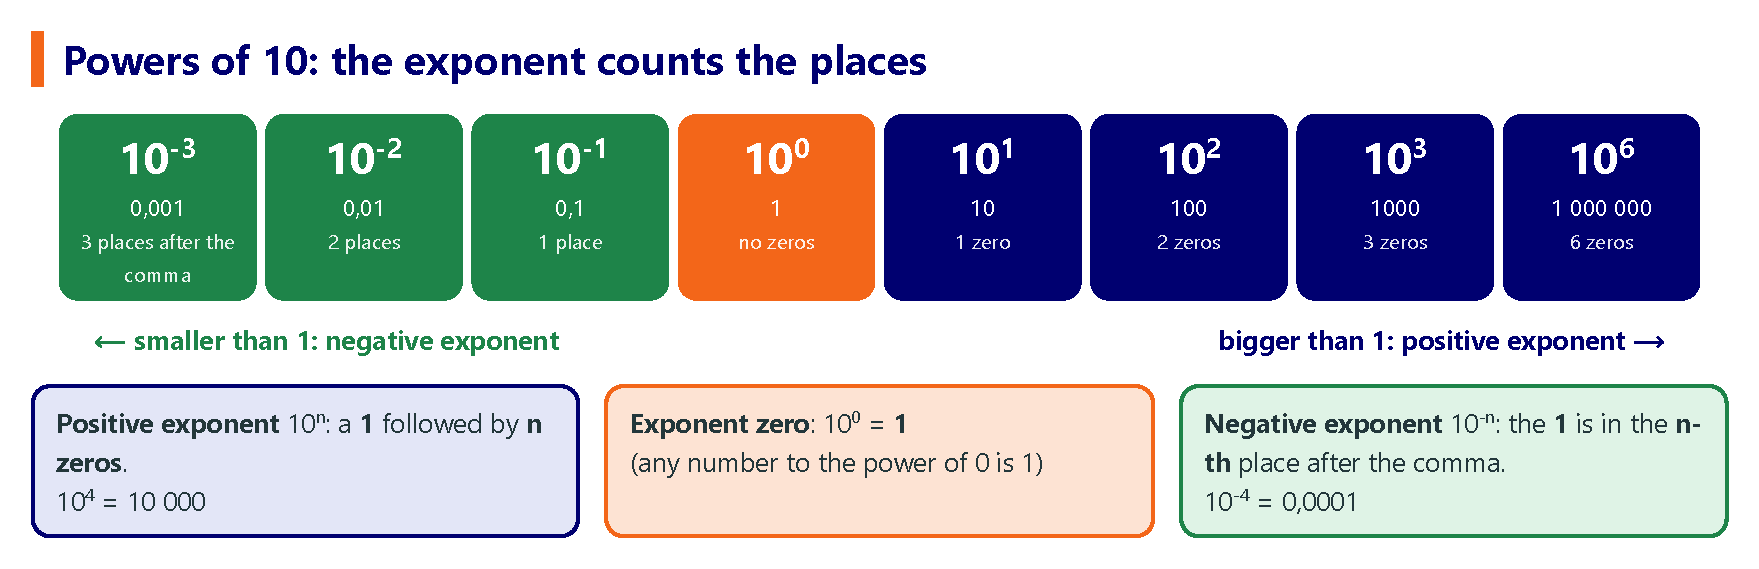
\includegraphics[width=\textwidth]{FigurasSVG/Unit_0_Math_Tools/pdf/power10_line.pdf}
    \caption{Positive exponents give numbers bigger than 1; negative exponents give numbers smaller than 1.}
    \label{fig:u0_power10_line}
\end{figure}

\begin{impt}
    \begin{itemize}
        \item \(10^{n}\) with \(n\) \textbf{positive}: a \textbf{1} followed by \textbf{\(n\) zeros}. \quad \(10^{5} = \num{100000}\).
        \item \(10^{0} = 1\).
        \item \(10^{-n}\) with \(n\) \textbf{positive}: a decimal number with the \textbf{1} in the \textbf{\(n\)-th place} after the comma. \quad \(10^{-5} = \num{0.00001}\).
    \end{itemize}
\end{impt}

\subsection{Writing numbers with powers of 10, and back to decimal}

Any number can be written as a number multiplied by a power of 10. It is still \textbf{the same number}, only written in a different way:
\begin{equation*}
    \num{5000} = 5 \cdot \num{1000} = 5 \cdot 10^{3}
    \qquad\qquad
    \num{0.007} = 7 \cdot \num{0.001} = 7 \cdot 10^{-3}
\end{equation*}

\negsubro{From a power of 10 to decimal}: the exponent tells us how many places the comma moves.
\begin{itemize}
    \item \textbf{Positive} exponent: the comma moves to the \textbf{right} (the number gets bigger). If there are no more digits, we add zeros: \(\num{3.2e4} = 3{,}2 \to 32\,000\).
    \item \textbf{Negative} exponent: the comma moves to the \textbf{left} (the number gets smaller). If there are no more digits, we add zeros and a 0 in front of the comma: \(\num{4.5e-3} = \num{0.0045}\).
\end{itemize}

\begin{example}
    \textbf{Write as a power of 10, and then go back to decimal.}
    \begin{itemize}
        \item \(\num{1000000} = 10^{6}\) (a 1 and six zeros). Back: \(10^{6}\) \(\to\) 1 followed by 6 zeros \(= \num{1000000}\).
        \item \(\num{0.01} = 10^{-2}\) (the 1 is in the 2nd place after the comma). Back: \(10^{-2} = \num{0.01}\).
        \item \(\num{80000} = 8 \cdot 10^{4}\). Back: \(8 \cdot 10^{4}\) \(\to\) the comma of 8 moves 4 places to the right: \(\num{80000}\).
        \item \(\num{0.0006} = 6 \cdot 10^{-4}\). Back: \(6 \cdot 10^{-4}\) \(\to\) the comma of 6 moves 4 places to the left: \(\num{0.0006}\).
    \end{itemize}
\end{example}

\begin{exercise}
    Write these numbers as a power of 10 (or as a number times a power of 10):
    \begin{enumerate}[label=\letraminuscula]
        \item \num{10000}
        \item \num{0.001}
        \item \num{100000000}
        \item \num{0.000001}
        \item \num{3000}
        \item \num{0.05}
        \item \num{7000000}
        \item \num{0.0009}
    \end{enumerate}
    \begin{solu}
        a) \(10^{4}\); b) \(10^{-3}\); c) \(10^{8}\); d) \(10^{-6}\); e) \(3 \cdot 10^{3}\); f) \(5 \cdot 10^{-2}\); g) \(7 \cdot 10^{6}\); h) \(9 \cdot 10^{-4}\).
    \end{solu}
\end{exercise}

\begin{exercise}
    Write these numbers as decimal numbers:
    \begin{enumerate}[label=\letraminuscula]
        \item \(10^{3}\)
        \item \(10^{-4}\)
        \item \(2 \cdot 10^{5}\)
        \item \(6{,}5 \cdot 10^{2}\)
        \item \(3 \cdot 10^{-2}\)
        \item \(1{,}2 \cdot 10^{-3}\)
    \end{enumerate}
    \begin{solu}
        a) \num{1000}; b) \num{0.0001}; c) \num{200000}; d) \num{650}; e) \num{0.03}; f) \num{0.0012}.
    \end{solu}
\end{exercise}

\subsection{The rules of powers of 10}

\begin{figure}[H]
    \centering
    % [FIGURA ORIGINAL] \includegraphics[width=\textwidth]{Unit_0/power10_rules}
    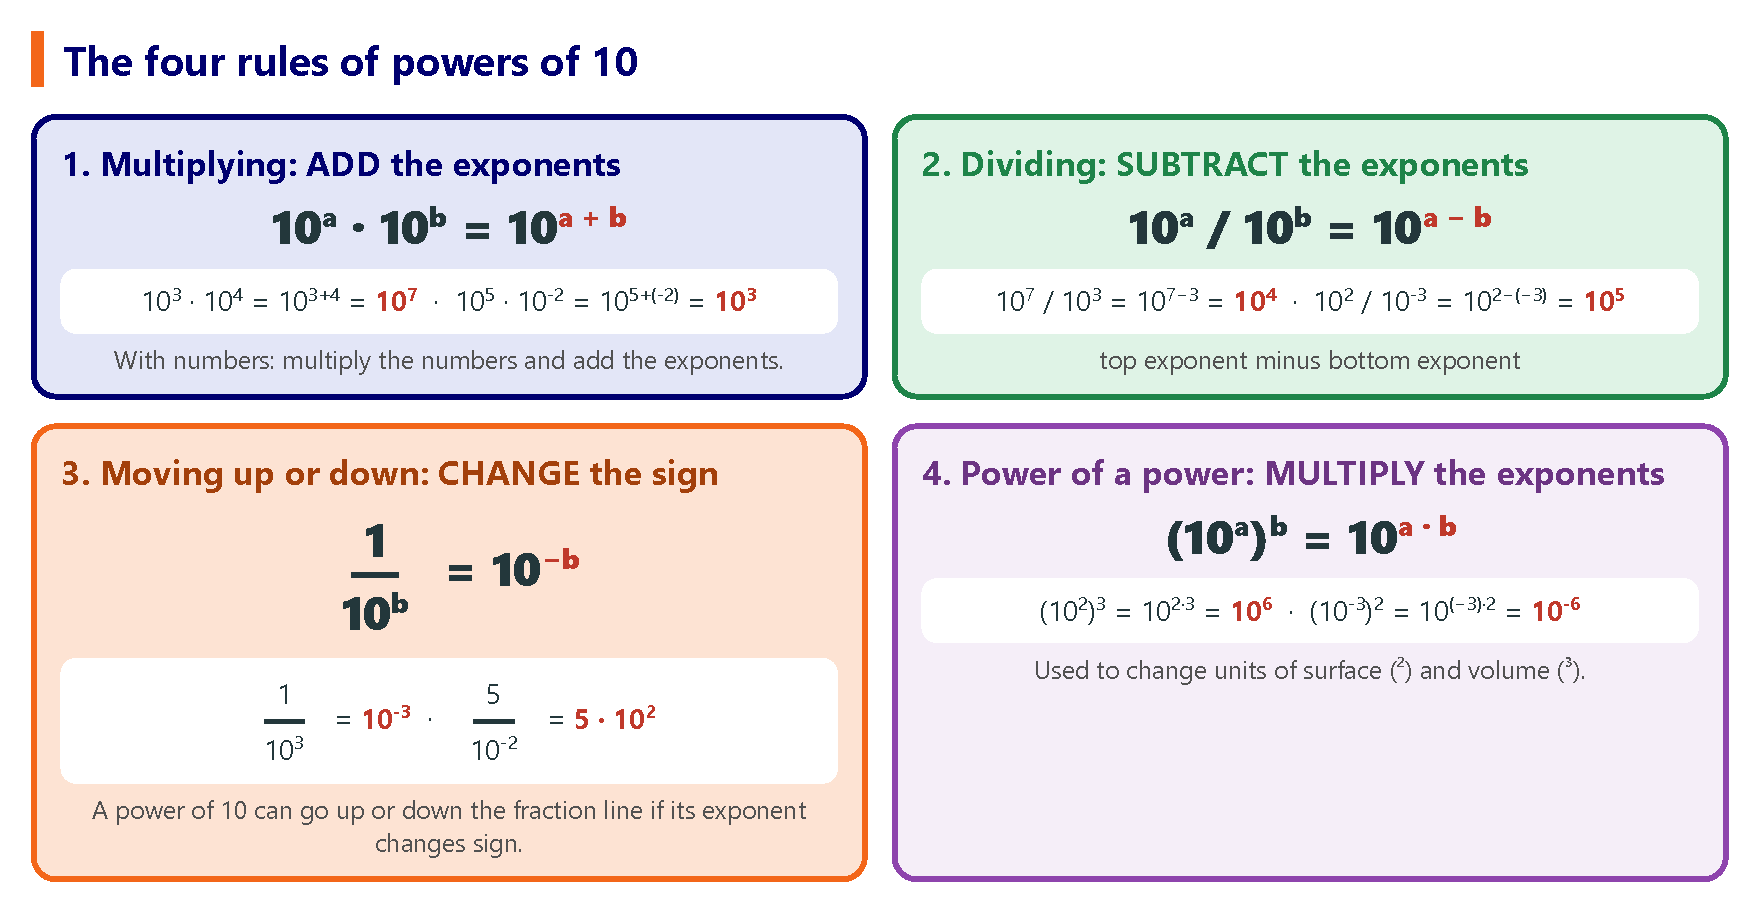
\includegraphics[width=\textwidth]{FigurasSVG/Unit_0_Math_Tools/pdf/power10_rules.pdf}
    \caption{The four rules for operating with powers of 10.}
    \label{fig:u0_power10_rules}
\end{figure}

\subsubsection{Multiplying: we add the exponents}

\begin{equation*}
    10^{a} \cdot 10^{b} = 10^{a+b}
\end{equation*}

If the powers of 10 have a number in front, we multiply the numbers on one side and the powers of 10 on the other:

\begin{example}
    \begin{itemize}
        \item \(10^{3} \cdot 10^{5} = 10^{3+5} = \textcolor{red}{10^{8}}\)
        \item \(10^{6} \cdot 10^{-2} = 10^{6+(-2)} = \textcolor{red}{10^{4}}\)
        \item \((3 \cdot 10^{4}) \cdot (2 \cdot 10^{3}) = (3 \cdot 2) \cdot 10^{4+3} = \textcolor{red}{6 \cdot 10^{7}}\)
        \item \((5 \cdot 10^{-3}) \cdot (4 \cdot 10^{6}) = 20 \cdot 10^{3} = \textcolor{red}{2 \cdot 10^{4}}\)
    \end{itemize}
\end{example}

\subsubsection{Dividing: we subtract the exponents}

\begin{equation*}
    \dfrac{10^{a}}{10^{b}} = 10^{a-b}
\end{equation*}

We subtract: exponent of the top \textbf{minus} exponent of the bottom. Be careful with the signs!

\begin{example}
    \begin{itemize}
        \item \(\dfrac{10^{8}}{10^{3}} = 10^{8-3} = \textcolor{red}{10^{5}}\)
        \item \(\dfrac{10^{2}}{10^{-4}} = 10^{2-(-4)} = 10^{2+4} = \textcolor{red}{10^{6}}\)
        \item \(\dfrac{8 \cdot 10^{6}}{2 \cdot 10^{2}} = \dfrac{8}{2} \cdot 10^{6-2} = \textcolor{red}{4 \cdot 10^{4}}\)
        \item \(\dfrac{9 \cdot 10^{-3}}{3 \cdot 10^{2}} = 3 \cdot 10^{-3-2} = \textcolor{red}{3 \cdot 10^{-5}}\)
    \end{itemize}
\end{example}

\subsubsection{Moving a power of 10 up or down: we change the sign of the exponent}

A power of 10 that is \textbf{below} the fraction line can be moved \textbf{above} it (and the other way round) if we \textbf{change the sign} of its exponent:
\begin{equation*}
    \dfrac{1}{10^{b}} = 10^{-b}
    \qquad\qquad
    10^{-b} = \dfrac{1}{10^{b}}
\end{equation*}

\begin{figure}[H]
    \centering
    % [FIGURA ORIGINAL] \includegraphics[width=\textwidth]{Unit_0/power10_flip}
    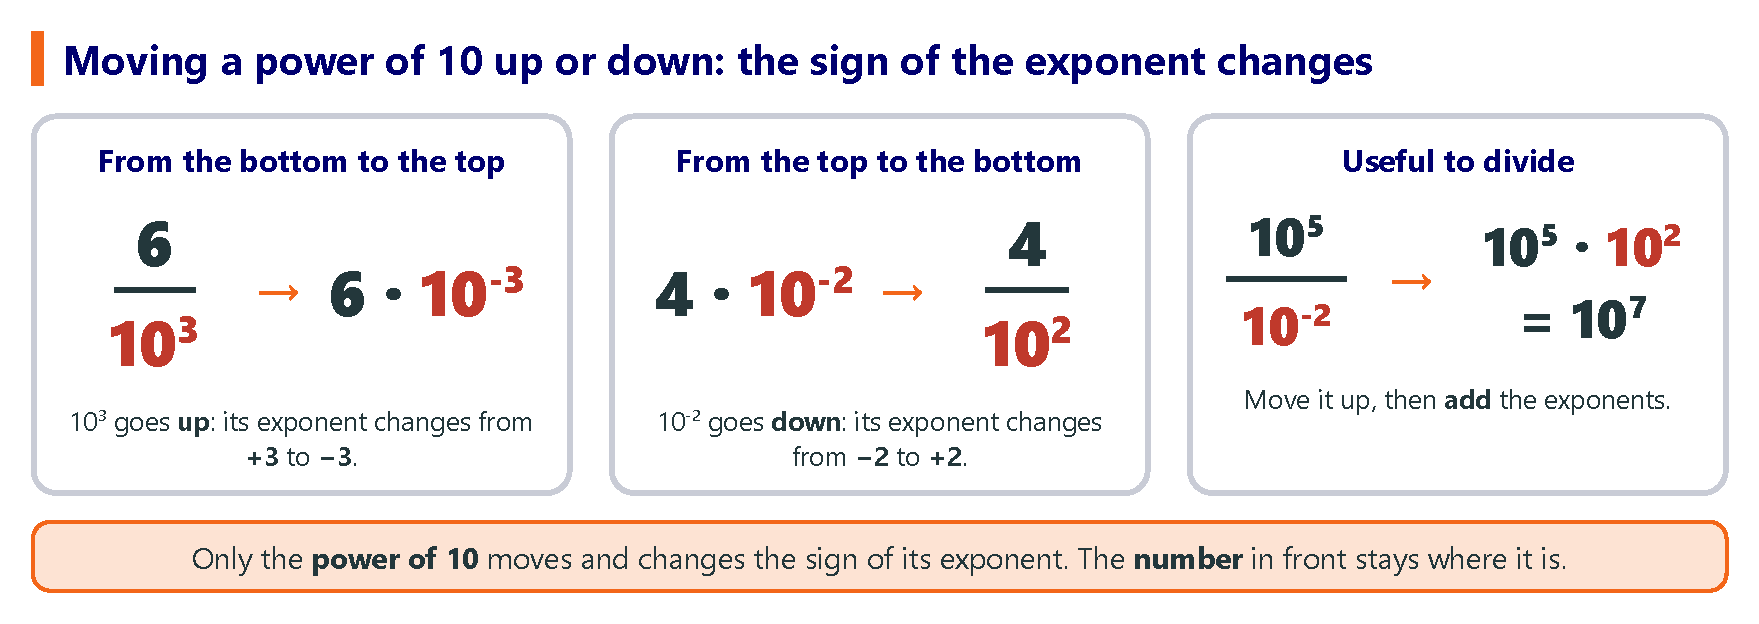
\includegraphics[width=\textwidth]{FigurasSVG/Unit_0_Math_Tools/pdf/power10_flip.pdf}
    \caption{When a power of 10 crosses the fraction line, its exponent changes sign.}
    \label{fig:u0_power10_flip}
\end{figure}

\begin{example}
    \begin{itemize}
        \item \(\dfrac{6}{10^{3}} = \textcolor{red}{6 \cdot 10^{-3}}\) \quad (\(10^{3}\) goes up as \(10^{-3}\))
        \item \(\dfrac{7}{10^{-2}} = \textcolor{red}{7 \cdot 10^{2}}\) \quad (\(10^{-2}\) goes up as \(10^{2}\))
        \item \(\dfrac{10^{5}}{10^{-2}} = 10^{5} \cdot 10^{2} = \textcolor{red}{10^{7}}\) \quad (we move it up and then add the exponents; it is the same result as subtracting \(5 - (-2) = 7\))
        \item This is very useful with conversion factors: \(\num{450}\,\unit{\mg} \cdot \dfrac{\qty{1}{\g}}{\qty{e3}{\mg}} = 450 \cdot 10^{-3}\,\unit{\g} = \qty{0.45}{\g}\).
    \end{itemize}
\end{example}

\subsubsection{Power of a power: we multiply the exponents}

\begin{equation*}
    \left(10^{a}\right)^{b} = 10^{a \cdot b}
\end{equation*}

If there is a number in front, it is also raised to the power: \(\left(3 \cdot 10^{2}\right)^{2} = 3^{2} \cdot 10^{2 \cdot 2} = 9 \cdot 10^{4}\).

\begin{example}
    \begin{itemize}
        \item \(\left(10^{3}\right)^{2} = 10^{3 \cdot 2} = \textcolor{red}{10^{6}}\)
        \item \(\left(10^{-2}\right)^{3} = 10^{(-2) \cdot 3} = \textcolor{red}{10^{-6}}\)
        \item \(\left(2 \cdot 10^{4}\right)^{3} = 2^{3} \cdot 10^{4 \cdot 3} = \textcolor{red}{8 \cdot 10^{12}}\)
        \item This is what we do when we change units of volume: \(\left(\dfrac{\qty{e2}{\cm}}{\qty{1}{\m}}\right)^{3} = \dfrac{10^{2 \cdot 3}\,\unit{\cubic\cm}}{\qty{1}{\cubic\m}} = \dfrac{\qty{e6}{\cubic\cm}}{\qty{1}{\cubic\m}}\).
    \end{itemize}
\end{example}

\begin{exercise}
    \textbf{Multiplying.} Calculate and leave the result as a power of 10:
    \begin{enumerate}[label=\letraminuscula]
        \item \(10^{4} \cdot 10^{2}\)
        \item \(10^{-3} \cdot 10^{-5}\)
        \item \(10^{7} \cdot 10^{-4}\)
        \item \((2 \cdot 10^{3}) \cdot (4 \cdot 10^{5})\)
        \item \((3 \cdot 10^{-2}) \cdot (3 \cdot 10^{6})\)
        \item \((5 \cdot 10^{4}) \cdot (6 \cdot 10^{-7})\)
    \end{enumerate}
    \begin{solu}
        a) \(10^{6}\); b) \(10^{-8}\); c) \(10^{3}\); d) \(8 \cdot 10^{8}\); e) \(9 \cdot 10^{4}\); f) \(30 \cdot 10^{-3} = 3 \cdot 10^{-2}\).
    \end{solu}
\end{exercise}

\begin{exercise}
    \textbf{Dividing.} Calculate and leave the result as a power of 10:
    \begin{enumerate}[label=\letraminuscula]
        \item \(\dfrac{10^{9}}{10^{4}}\)
        \item \(\dfrac{10^{3}}{10^{-2}}\)
        \item \(\dfrac{10^{-4}}{10^{2}}\)
        \item \(\dfrac{6 \cdot 10^{8}}{3 \cdot 10^{5}}\)
        \item \(\dfrac{8 \cdot 10^{-2}}{4 \cdot 10^{-6}}\)
        \item \(\dfrac{12 \cdot 10^{3}}{4 \cdot 10^{7}}\)
    \end{enumerate}
    \begin{solu}
        a) \(10^{5}\); b) \(10^{5}\); c) \(10^{-6}\); d) \(2 \cdot 10^{3}\); e) \(2 \cdot 10^{4}\); f) \(3 \cdot 10^{-4}\).
    \end{solu}
\end{exercise}

\begin{exercise}
    \textbf{Moving up.} Write without fractions, moving the power of 10 to the top:
    \begin{enumerate}[label=\letraminuscula]
        \item \(\dfrac{1}{10^{4}}\)
        \item \(\dfrac{3}{10^{2}}\)
        \item \(\dfrac{5}{10^{-3}}\)
        \item \(\dfrac{10^{2}}{10^{-5}}\)
    \end{enumerate}
    \begin{solu}
        a) \(10^{-4}\); b) \(3 \cdot 10^{-2}\); c) \(5 \cdot 10^{3}\); d) \(10^{2} \cdot 10^{5} = 10^{7}\).
    \end{solu}
\end{exercise}

\begin{exercise}
    \textbf{Power of a power.} Calculate:
    \begin{enumerate}[label=\letraminuscula]
        \item \(\left(10^{4}\right)^{2}\)
        \item \(\left(10^{-1}\right)^{3}\)
        \item \(\left(10^{-3}\right)^{-2}\)
        \item \(\left(3 \cdot 10^{2}\right)^{3}\)
        \item \(\left(\dfrac{\qty{e3}{\mm}}{\qty{1}{\m}}\right)^{2}\)
    \end{enumerate}
    \begin{solu}
        a) \(10^{8}\); b) \(10^{-3}\); c) \(10^{6}\); d) \(27 \cdot 10^{6} = 2{,}7 \cdot 10^{7}\); e) \(\dfrac{\qty{e6}{\square\mm}}{\qty{1}{\square\m}}\).
    \end{solu}
\end{exercise}

\begin{exercise}
    \textbf{Mixed.} Calculate, leaving the result as a power of 10, and then write it as a decimal number:
    \begin{enumerate}[label=\letraminuscula]
        \item \(\dfrac{10^{3} \cdot 10^{4}}{10^{5}}\)
        \item \(\dfrac{10^{-2} \cdot 10^{6}}{10^{-1}}\)
        \item \(\dfrac{(2 \cdot 10^{3})^{2}}{4 \cdot 10^{2}}\)
    \end{enumerate}
    \begin{solu}
        a) \(\dfrac{10^{7}}{10^{5}} = 10^{2} = 100\); \quad
        b) \(\dfrac{10^{4}}{10^{-1}} = 10^{5} = \num{100000}\); \quad
        c) \(\dfrac{4 \cdot 10^{6}}{4 \cdot 10^{2}} = 10^{4} = \num{10000}\).
    \end{solu}
\end{exercise}

%----------------------------------------------------------------------------------------

\section{Equations: how to isolate a quantity}

\subsection{What does isolating mean?}

In science, formulas link several quantities: \(d = \dfrac{m}{V}\), \(v = \dfrac{x}{t}\), \(F = m \cdot a\)\ldots{} Very often we know some of them and we want to calculate another one, which is not alone. Then we must \textbf{isolate} it.

\begin{definition}[Isolating a quantity]
    To \textbf{isolate} a quantity (\emph{despejar}) is to rearrange an equation so that this quantity is \textbf{completely alone} on one side of the equals sign, \textbf{in the numerator}, and everything else is on the other side.
\end{definition}

\begin{figure}[H]
    \centering
    % [FIGURA ORIGINAL] \includegraphics[width=\textwidth]{Unit_0/isolate_meaning}
    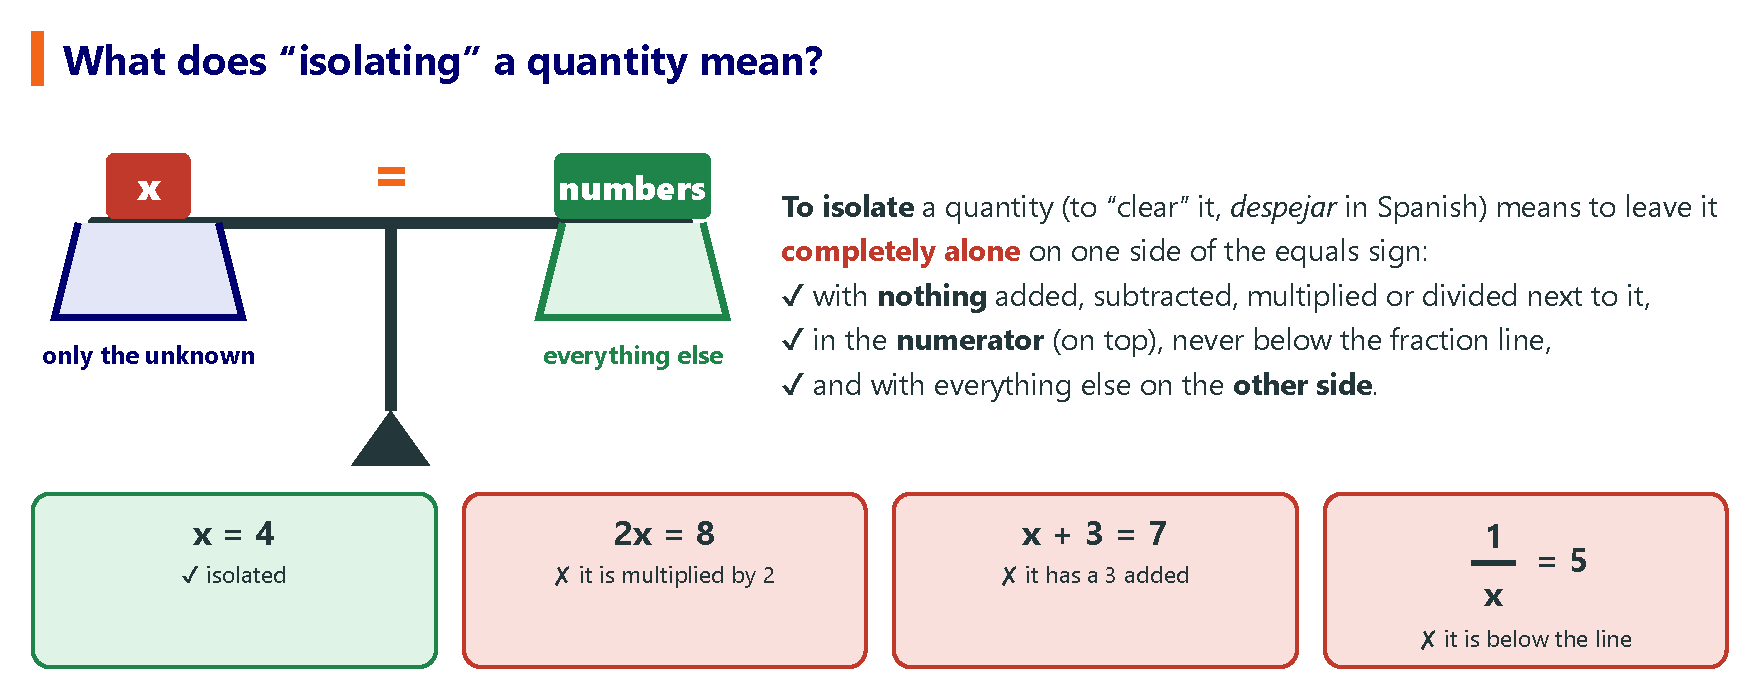
\includegraphics[width=\textwidth]{FigurasSVG/Unit_0_Math_Tools/pdf/isolate_meaning.pdf}
    \caption{An equation is like a balanced scale. Isolating means leaving the unknown alone on one side.}
    \label{fig:u0_isolate_meaning}
\end{figure}

An equation is like a \textbf{balanced scale}: the two sides are equal. If we do the \textbf{same operation on both sides}, the scale stays balanced and the equation is still true. We use this to remove, one by one, everything that is next to the unknown.

\subsection{Two methods to isolate}

\begin{figure}[H]
    \centering
    % [FIGURA ORIGINAL] \includegraphics[width=\textwidth]{Unit_0/isolate_shortcut}
    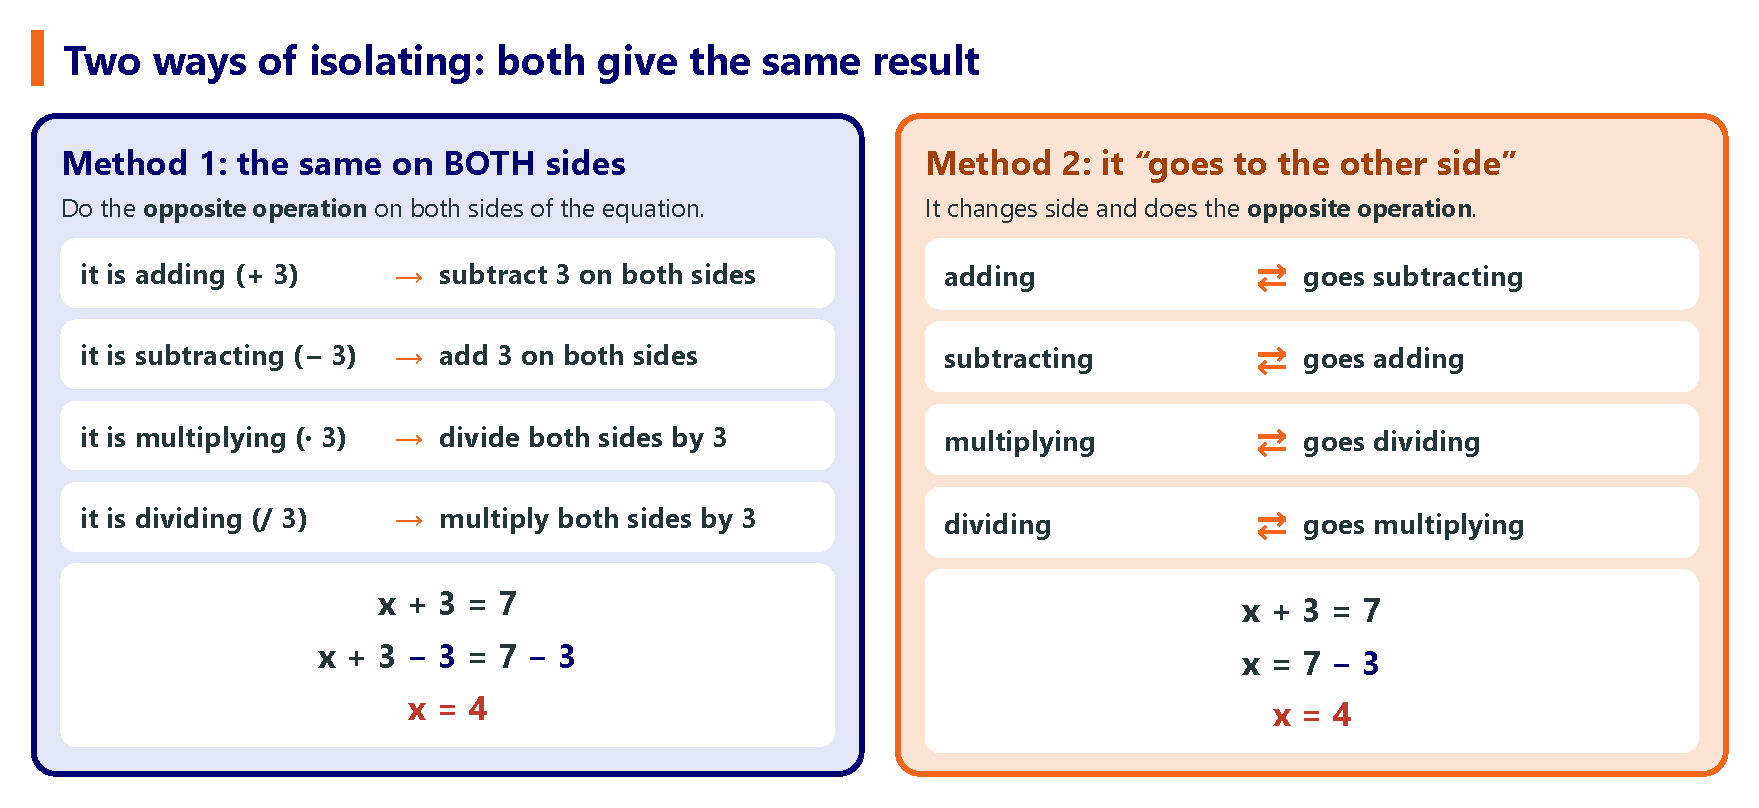
\includegraphics[width=\textwidth]{FigurasSVG/Unit_0_Math_Tools/pdf/isolate_shortcut.pdf}
    \caption{Method 1 (the same operation on both sides) and Method 2 (going to the other side) give the same result.}
    \label{fig:u0_isolate_shortcut}
\end{figure}

\negsubro{Method 1: the same operation on both sides} (the method of mathematics). We look at what is ``stuck'' to the unknown and we do the \textbf{opposite operation on both sides}:
\begin{itemize}
    \item If it is \textbf{adding}, we \textbf{subtract} it on both sides.
    \item If it is \textbf{subtracting}, we \textbf{add} it on both sides.
    \item If it is \textbf{multiplying}, we \textbf{divide} both sides by it.
    \item If it is \textbf{dividing}, we \textbf{multiply} both sides by it.
\end{itemize}

\negsubro{Method 2: going to the other side} (the shortcut). A quantity can \textbf{change side} if it also \textbf{changes its operation} to the opposite one:
\begin{center}
    \renewcommand{\arraystretch}{1.3}
    \begin{tabular}{ccc}
        \toprule
        \textbf{If it is\ldots} & & \textbf{it goes to the other side\ldots} \\
        \midrule
        adding \((+)\) & \(\longleftrightarrow\) & subtracting \((-)\) \\
        subtracting \((-)\) & \(\longleftrightarrow\) & adding \((+)\) \\
        multiplying \((\cdot)\) & \(\longleftrightarrow\) & dividing \((/)\) \\
        dividing \((/)\) & \(\longleftrightarrow\) & multiplying \((\cdot)\) \\
        \bottomrule
    \end{tabular}
\end{center}

\begin{impt}
    Method 2 is just a quick way of writing Method 1: when we ``pass'' the 3 subtracting, we are really subtracting 3 on both sides. Use the method you understand best, but \textbf{never} change the operation without changing the side!
\end{impt}

\subsection{Examples with both methods}

\begin{example}
    \textbf{Adding: \(x + 5 = 12\).}
    \begin{itemize}
        \item Method 1: we subtract 5 on both sides: \(x + 5 \textcolor{blue}{- 5} = 12 \textcolor{blue}{- 5}\) \(\Rightarrow\) \(\textcolor{red}{x = 7}\).
        \item Method 2: the 5 is adding, so it goes to the other side subtracting: \(x = 12 - 5\) \(\Rightarrow\) \(\textcolor{red}{x = 7}\).
    \end{itemize}
\end{example}

\begin{example}
    \textbf{Subtracting: \(x - 3 = 10\).}
    \begin{itemize}
        \item Method 1: we add 3 on both sides: \(x - 3 \textcolor{blue}{+ 3} = 10 \textcolor{blue}{+ 3}\) \(\Rightarrow\) \(\textcolor{red}{x = 13}\).
        \item Method 2: the 3 is subtracting, so it goes to the other side adding: \(x = 10 + 3\) \(\Rightarrow\) \(\textcolor{red}{x = 13}\).
    \end{itemize}
\end{example}

\begin{example}
    \textbf{Multiplying: \(4 \cdot x = 20\).}
    \begin{itemize}
        \item Method 1: we divide both sides by 4: \(\dfrac{\cancelred{4} \cdot x}{\cancelred{4}} = \dfrac{20}{4}\) \(\Rightarrow\) \(\textcolor{red}{x = 5}\).
        \item Method 2: the 4 is multiplying, so it goes to the other side dividing: \(x = \dfrac{20}{4}\) \(\Rightarrow\) \(\textcolor{red}{x = 5}\).
    \end{itemize}
\end{example}

\begin{example}
    \textbf{Dividing: \(\dfrac{x}{3} = 6\).}
    \begin{itemize}
        \item Method 1: we multiply both sides by 3: \(\dfrac{x \cdot \cancelred{3}}{\cancelred{3}} = 6 \cdot 3\) \(\Rightarrow\) \(\textcolor{red}{x = 18}\).
        \item Method 2: the 3 is dividing, so it goes to the other side multiplying: \(x = 6 \cdot 3\) \(\Rightarrow\) \(\textcolor{red}{x = 18}\).
    \end{itemize}
\end{example}

\begin{example}
    \textbf{Two steps: \(2 \cdot x + 3 = 11\).} First we remove what is \textbf{added or subtracted}, and then what is \textbf{multiplying or dividing}:
    \begin{enumerate}[label=\numberballmDarkTeal]
        \item The 3 is adding: it goes to the other side subtracting: \(2 \cdot x = 11 - 3 = 8\).
        \item The 2 is multiplying: it goes to the other side dividing: \(x = \dfrac{8}{2}\) \(\Rightarrow\) \(\textcolor{red}{x = 4}\).
        \item Check: \(2 \cdot 4 + 3 = 11\). \textcolor{green!50!black}{Correct!}
    \end{enumerate}
\end{example}

\begin{marker}
    \textbf{Always check your result}: put the value you have found back into the original equation. If both sides are equal, it is correct.
\end{marker}

\subsection{When the unknown is below the fraction line}

Sometimes the quantity we want to isolate is in the \textbf{denominator}, for example the time \(t\) in \(v = \dfrac{x}{t}\) or the volume \(V\) in \(d = \dfrac{m}{V}\). In this case, \textbf{the first step is always to bring it up}: we multiply both sides by it (it ``goes up multiplying'').

\begin{impt}
    If we do not bring the unknown up first, it stays in the denominator and what we get is \(\dfrac{1}{x}\), \textbf{not} \(x\). And \(\dfrac{1}{x}\) is \textbf{not} the same as \(x\): if \(\dfrac{1}{x} = 0{,}25\), then \(x = 4\), not \(0{,}25\)!
\end{impt}

\begin{figure}[H]
    \centering
    % [FIGURA ORIGINAL] \includegraphics[width=\textwidth]{Unit_0/denominator_up}
    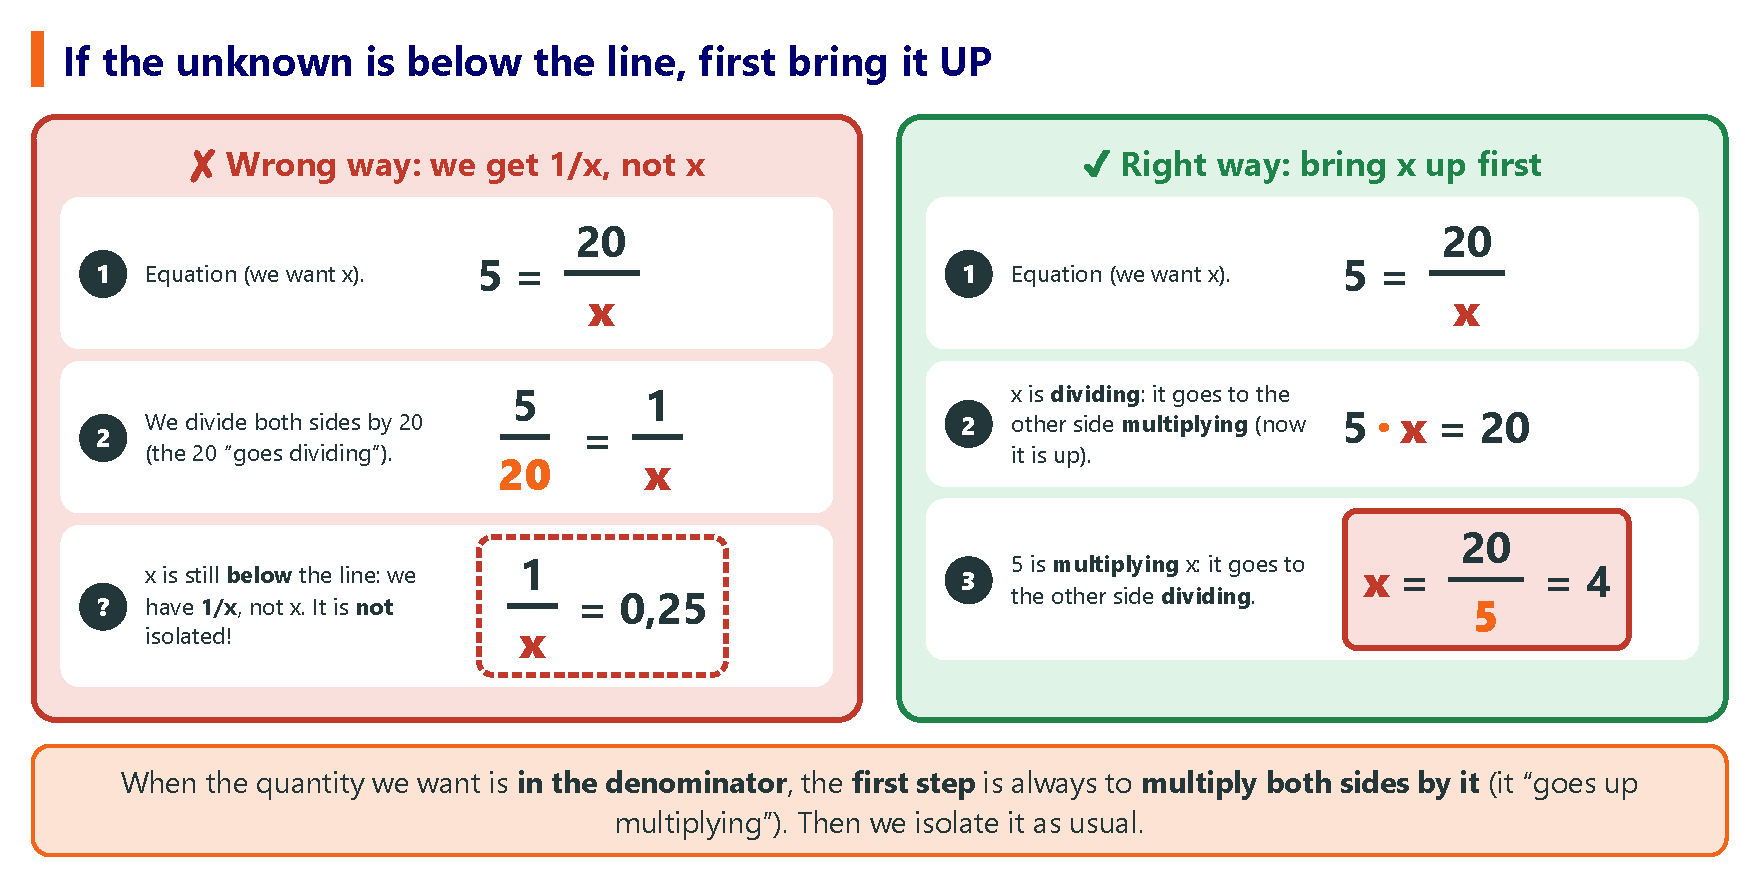
\includegraphics[width=\textwidth]{FigurasSVG/Unit_0_Math_Tools/pdf/denominator_up.pdf}
    \caption{If the unknown is in the denominator, we must first bring it up (multiplying); otherwise we get 1/x instead of x.}
    \label{fig:u0_denominator_up}
\end{figure}

\begin{example}
    \textbf{Isolate \(t\) in \(v = \dfrac{x}{t}\).}
    \begin{enumerate}[label=\numberballmDarkTeal]
        \item \(t\) is below the line, dividing: we bring it up multiplying (we multiply both sides by \(t\)): \(v \cdot t = x\).
        \item Now \(v\) is multiplying \(t\): it goes to the other side dividing: \(\textcolor{red}{t = \dfrac{x}{v}}\).
    \end{enumerate}
\end{example}

\begin{example}
    \textbf{Isolate \(V\) in \(d = \dfrac{m}{V}\), and calculate it for \(m = \qty{60}{\g}\) and \(d = \qty{3}{\g\per\cubic\cm}\).}
    \begin{enumerate}[label=\numberballmDarkTeal]
        \item \(V\) is below the line: it goes up multiplying: \(d \cdot V = m\).
        \item \(d\) is multiplying \(V\): it goes to the other side dividing: \(V = \dfrac{m}{d}\).
        \item \(V = \dfrac{\qty{60}{\g}}{\qty{3}{\g\per\cubic\cm}} = \textcolor{red}{\qty{20}{\cubic\cm}}\).
    \end{enumerate}
\end{example}

\subsection{Isolating in the formulas of physics and chemistry}

The method is exactly the same with letters as with numbers. Here are the formulas you will use most this year, with each quantity isolated:

\begin{table}[H]
    \centering
    \renewcommand{\arraystretch}{2.2}
    \begin{tabular}{llll}
        \toprule
        \textbf{Formula} & \multicolumn{3}{l}{\textbf{Isolated quantities}} \\
        \midrule
         \(d = \dfrac{m}{V}\) & \(m = d \cdot V\) & \(V = \dfrac{m}{d}\) & \\
        \(v = \dfrac{x}{t}\) & \(x = v \cdot t\) & \(t = \dfrac{x}{v}\) & \\
        \(F = m \cdot a\) & \(m = \dfrac{F}{a}\) & \(a = \dfrac{F}{m}\) & \\
        \(W = m \cdot g\) & \(m = \dfrac{W}{g}\) & \(g = \dfrac{W}{m}\) & \\
        \(T = t_{\text{C}} + 273\) & \(t_{\text{C}} = T - 273\) & & \\
        \(p_1 \cdot V_1 = p_2 \cdot V_2\) & \(V_2 = \dfrac{p_1 \cdot V_1}{p_2}\) & \(p_2 = \dfrac{p_1 \cdot V_1}{V_2}\) & \\
        \bottomrule
    \end{tabular}
    \caption{The most common formulas of the course, with each quantity isolated.}
    \label{tab:u0_formulas}
\end{table}

\begin{example}
    \textbf{Isolate \(v_f\) in \(a = \dfrac{v_f - v_i}{t}\).} Here the unknown is inside a subtraction that is divided by \(t\):
    \begin{enumerate}[label=\numberballmDarkTeal]
        \item \(t\) is dividing the whole subtraction: it goes to the other side multiplying: \(a \cdot t = v_f - v_i\).
        \item \(v_i\) is subtracting: it goes to the other side adding: \(\textcolor{red}{v_f = v_i + a \cdot t}\).
    \end{enumerate}
\end{example}

\begin{exercise}
    Isolate \(x\), using \textbf{both} methods, and check your result:
    \begin{enumerate}[label=\letraminuscula]
        \item \(x + 8 = 15\)
        \item \(x - 6 = 2\)
        \item \(5 \cdot x = 35\)
        \item \(\dfrac{x}{4} = 7\)
        \item \(3 \cdot x - 4 = 11\)
        \item \(\dfrac{x}{2} + 1 = 9\)
    \end{enumerate}
    \begin{solu}
        a) \(x = 15 - 8 = 7\); b) \(x = 2 + 6 = 8\); c) \(x = \dfrac{35}{5} = 7\); d) \(x = 7 \cdot 4 = 28\); e) \(3x = 11 + 4 = 15\), \(x = 5\); f) \(\dfrac{x}{2} = 9 - 1 = 8\), \(x = 16\).
    \end{solu}
\end{exercise}

\begin{exercise}
    The unknown is in the denominator. Bring it up first, and then isolate it:
    \begin{enumerate}[label=\letraminuscula]
        \item \(6 = \dfrac{30}{x}\)
        \item \(\dfrac{12}{x} = 4\)
        \item \(0{,}5 = \dfrac{2}{x}\)
        \item \(\dfrac{100}{x} = 25\)
    \end{enumerate}
    \begin{solu}
        a) \(6x = 30\), \(x = 5\); b) \(12 = 4x\), \(x = 3\); c) \(0{,}5x = 2\), \(x = 4\); d) \(100 = 25x\), \(x = 4\).
    \end{solu}
\end{exercise}

\begin{exercise}
    Isolate the quantity in brackets:
    \begin{enumerate}[label=\letraminuscula]
        \item \(d = \dfrac{m}{V}\) \quad (\(m\)) and (\(V\))
        \item \(v = \dfrac{x}{t}\) \quad (\(x\)) and (\(t\))
        \item \(F = m \cdot a\) \quad (\(a\))
        \item \(T = t_{\text{C}} + 273\) \quad (\(t_{\text{C}}\))
        \item \(\dfrac{V_1}{T_1} = \dfrac{V_2}{T_2}\) \quad (\(V_2\)) and (\(T_2\))
        \item \(a = \dfrac{v_f - v_i}{t}\) \quad (\(t\))
    \end{enumerate}
    \begin{solu}
        \begin{enumerate}[label=\alph*)]
            \item \(m = d \cdot V\); \(V = \dfrac{m}{d}\).
            \item \(x = v \cdot t\); \(t = \dfrac{x}{v}\).
            \item \(a = \dfrac{F}{m}\).
            \item \(t_{\text{C}} = T - 273\).
            \item \(V_2 = \dfrac{V_1 \cdot T_2}{T_1}\); \(T_2 = \dfrac{V_2 \cdot T_1}{V_1}\) (cross-multiply first: \(V_1 \cdot T_2 = V_2 \cdot T_1\)).
            \item \(t\) is in the denominator: \(a \cdot t = v_f - v_i\), so \(t = \dfrac{v_f - v_i}{a}\).
        \end{enumerate}
    \end{solu}
\end{exercise}

\begin{exercise}
    Isolate the unknown and calculate:
    \begin{enumerate}[label=\letraminuscula]
        \item The mass of a stone with \(V = \qty{50}{\cubic\cm}\) and \(d = \qty{2.6}{\g\per\cubic\cm}\).
        \item The time a car moving at \(v = \qty{20}{\mps}\) takes to travel \(x = \qty{900}{\m}\).
        \item The acceleration of a \(\qty{40}{\kg}\) trolley pushed with \(F = \qty{100}{\newton}\).
    \end{enumerate}
    \begin{solu}
        a) \(m = d \cdot V = \qty{2.6}{\g\per\cubic\cm} \cdot \qty{50}{\cubic\cm} = \qty{130}{\g}\); \quad
        b) \(t = \dfrac{x}{v} = \dfrac{\qty{900}{\m}}{\qty{20}{\mps}} = \qty{45}{\s}\); \quad
        c) \(a = \dfrac{F}{m} = \dfrac{\qty{100}{\newton}}{\qty{40}{\kg}} = \qty{2.5}{\mpss}\).
    \end{solu}
\end{exercise}

%----------------------------------------------------------------------------------------

\section{Graphs}

\subsection{The axes of a graph}

A graph has two perpendicular lines, called \textbf{axes}, that cross at the \textbf{origin} (0, 0):
\begin{itemize}
    \item The \textbf{horizontal axis} (in mathematics, the \(x\)-axis or \textbf{abscissa}).
    \item The \textbf{vertical axis} (in mathematics, the \(y\)-axis or \textbf{ordinate}).
\end{itemize}
Each point of the graph is written as \((\text{horizontal value}, \text{vertical value})\): the point \((3, 5)\) is 3 units to the right and 5 units up.

\begin{impt}
    \negsubro{In science, the axes do not have to be called \(x\) and \(y\)}. Each axis takes the name (and the unit) of the \textbf{quantity} we represent on it: \(t\) (s), \(v\) (m/s), \(m\) (g), \(T\) (\unit{\celsius})\ldots{} When we say ``\textbf{A vs B}'' (A \emph{versus} B), \textbf{A goes on the vertical axis} and \textbf{B goes on the horizontal axis}:
    \begin{itemize}
        \item ``\(v\) vs \(t\)'': \(v\) on the vertical axis and \(t\) on the horizontal axis.
        \item ``\(x\) vs \(t\)'': \(x\) on the vertical axis and \(t\) on the horizontal axis. Be careful: here \(x\) goes on the \textbf{vertical} axis!
        \item ``\(m\) vs \(V\)'': \(m\) on the vertical axis and \(V\) on the horizontal axis.
    \end{itemize}
    The time is almost always on the \textbf{horizontal} axis.
\end{impt}

\begin{figure}[H]
    \centering
    % [FIGURA ORIGINAL] \includegraphics[width=\textwidth]{Unit_0/axes_names}
    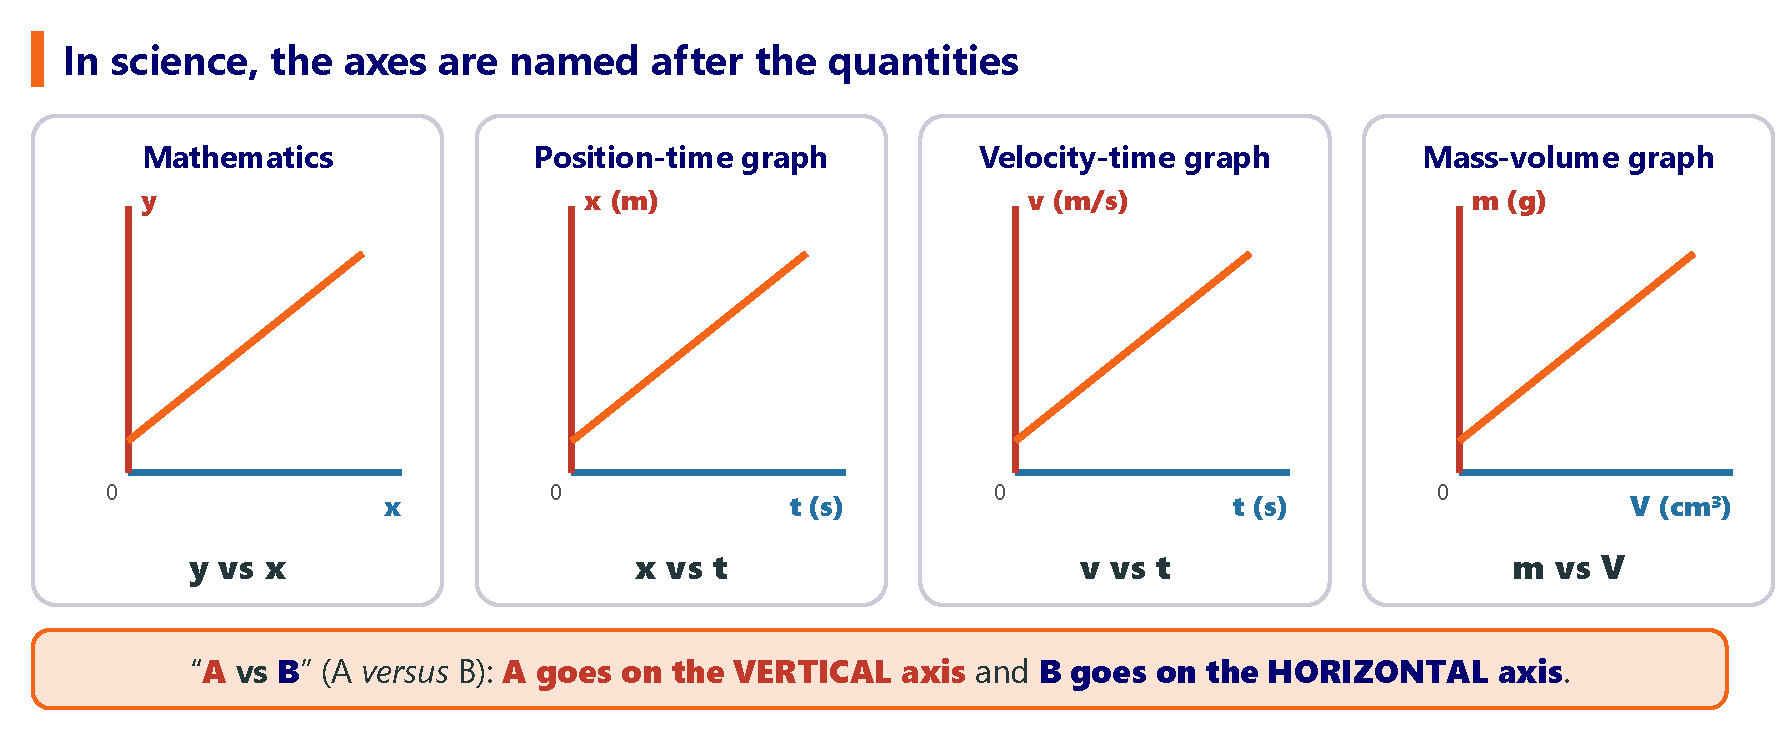
\includegraphics[width=\textwidth]{FigurasSVG/Unit_0_Math_Tools/pdf/axes_names.pdf}
    \caption{The same kind of graph with the axes named after different quantities.}
    \label{fig:u0_axes_names}
\end{figure}

\subsection{How to draw a graph from a table}

\negsubro{Method, step by step}:
\begin{enumerate}[label=\numberballmDarkTeal]
    \item Decide which quantity goes on each axis (``A vs B'': A vertical, B horizontal).
    \item Draw the axes and \textbf{label} them with the name of the quantity and its \textbf{unit}.
    \item Choose a \textbf{scale} for each axis, with equal steps (for example, every square is 2 s), so that all the values of the table fit.
    \item Plot each pair of values of the table as a \textbf{point}.
    \item If the points are in a straight line, join them with a \textbf{ruler}.
\end{enumerate}

\begin{example}
    \textbf{Mathematics: draw the graph of \(y = 2x + 1\).} First we make a table, giving values to \(x\):
    \begin{center}
        \begin{tabular}{lccccc}
            \toprule
            \(x\) & 0 & 1 & 2 & 3 & 4 \\
            \midrule
            \(y = 2x + 1\) & 1 & 3 & 5 & 7 & 9 \\
            \bottomrule
        \end{tabular}
    \end{center}
    \begin{center}
        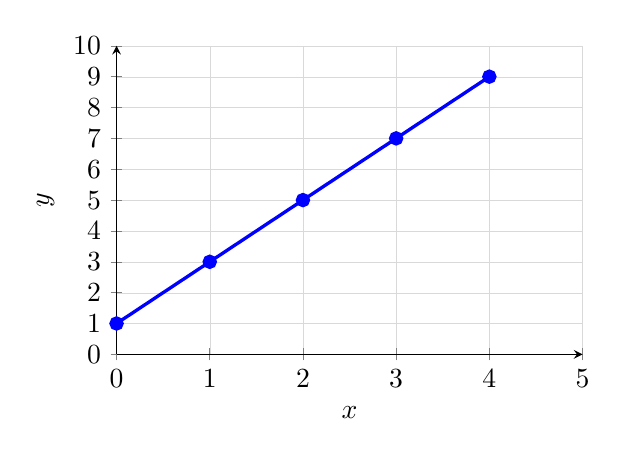
\begin{tikzpicture}
            \begin{axis}[width=7.5cm, height=5.5cm, grid=both, grid style={line width=.1pt, draw=gray!30},
                axis lines=left, xlabel={\(x\)}, ylabel={\(y\)}, xmin=0, xmax=5, ymin=0, ymax=10, xtick={0,1,...,5}, ytick={0,1,...,10}]
                \addplot[very thick, blue, mark=*] coordinates {(0,1) (1,3) (2,5) (3,7) (4,9)};
            \end{axis}
        \end{tikzpicture}
    \end{center}
\end{example}

\begin{example}
    \textbf{Science: draw the graph \(m\) vs \(V\) for pieces of aluminium.} Now the axes are called \(m\) (vertical) and \(V\) (horizontal), and each one has its unit:
    \begin{center}
        \begin{tabular}{lccccc}
            \toprule
            \(V\) (\unit{\cubic\cm}) & 0 & 10 & 20 & 30 & 40 \\
            \midrule
            \(m\) (\unit{\g}) & 0 & 27 & 54 & 81 & 108 \\
            \bottomrule
        \end{tabular}
    \end{center}
    \begin{center}
        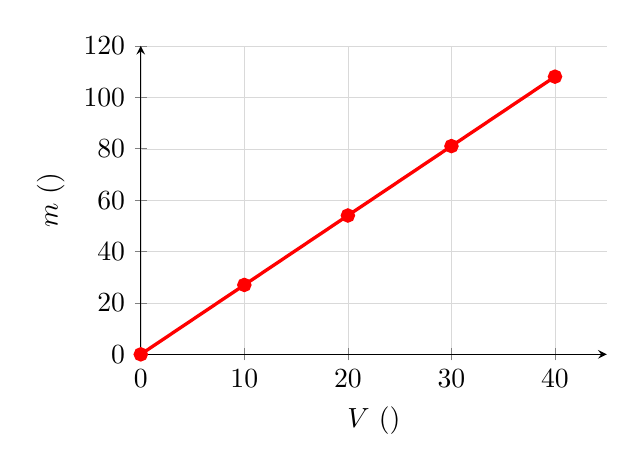
\begin{tikzpicture}
            \begin{axis}[width=7.5cm, height=5.5cm, grid=both, grid style={line width=.1pt, draw=gray!30},
                axis lines=left, xlabel={\(V\) (\unit{\cubic\cm})}, ylabel={\(m\) (\unit{\g})}, xmin=0, xmax=45, ymin=0, ymax=120, xtick={0,10,...,40}, ytick={0,20,...,120}]
                \addplot[very thick, red, mark=*] coordinates {(0,0) (10,27) (20,54) (30,81) (40,108)};
            \end{axis}
        \end{tikzpicture}
    \end{center}
    It is a straight line through the origin: the mass and the volume are \textbf{directly proportional}.
\end{example}

\subsection{Analysing straight-line graphs}

To read a straight-line graph we ask three questions:

\begin{figure}[H]
    \centering
    % [FIGURA ORIGINAL] \includegraphics[width=\textwidth]{Unit_0/slope}
    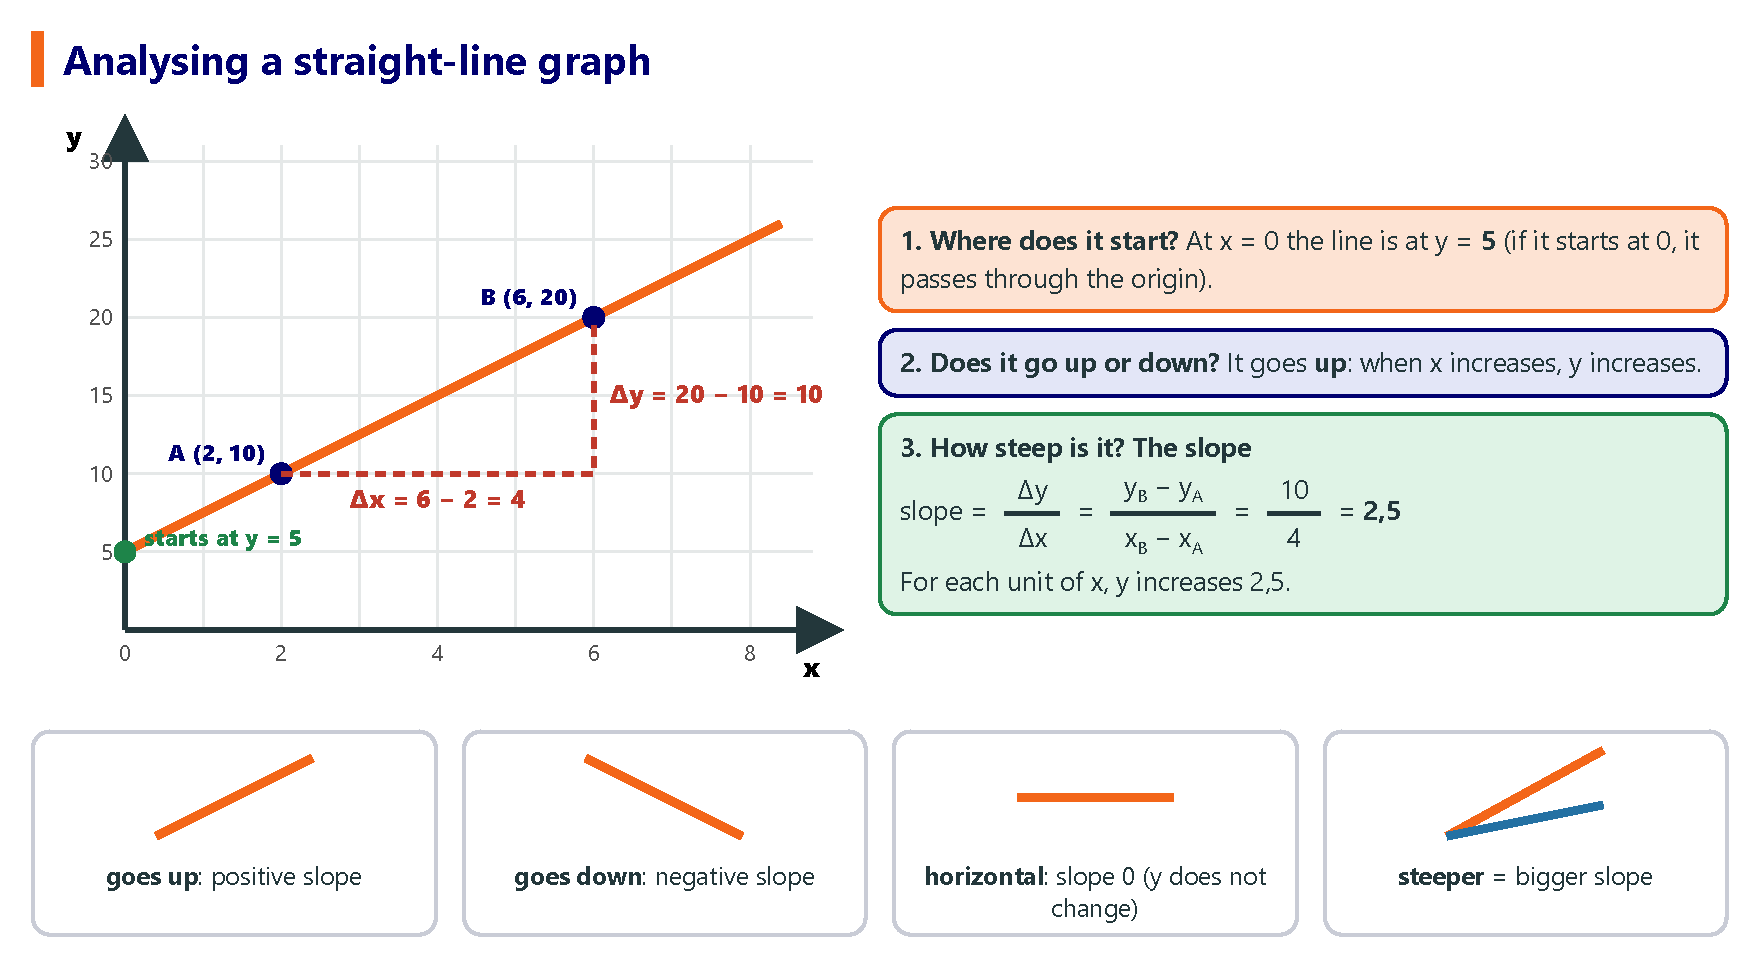
\includegraphics[width=\textwidth]{FigurasSVG/Unit_0_Math_Tools/pdf/slope.pdf}
    \caption{Where it starts, whether it goes up or down, and its slope.}
    \label{fig:u0_slope}
\end{figure}

\begin{enumerate}[label=\numberballmDarkTeal]
    \item \textbf{Where does it start?} The value on the vertical axis when the horizontal one is 0. If the line passes through \((0, 0)\), it starts at the \textbf{origin}.
    \item \textbf{Does it go up, go down or stay horizontal?} Going up means that the vertical quantity \textbf{increases}; going down, that it \textbf{decreases}; horizontal, that it \textbf{does not change}.
    \item \textbf{How steep is it?} This is the \negsubro{slope}: how much the vertical quantity changes for each unit of the horizontal one. We take two points \(A\) and \(B\) of the line:
    \begin{equation*}
        \text{slope} = \dfrac{\Delta(\text{vertical})}{\Delta(\text{horizontal})} = \dfrac{y_B - y_A}{x_B - x_A}
    \end{equation*}
\end{enumerate}

\begin{impt}
    \negsubro{In science the slope has a meaning}, and a unit:
    \begin{itemize}
        \item Slope of an \(x\) vs \(t\) graph \(= \dfrac{\Delta x}{\Delta t}\) = \textbf{velocity} (\unit{\mps}).
        \item Slope of a \(v\) vs \(t\) graph \(= \dfrac{\Delta v}{\Delta t}\) = \textbf{acceleration} (\unit{\mpss}).
        \item Slope of an \(m\) vs \(V\) graph \(= \dfrac{\Delta m}{\Delta V}\) = \textbf{density} (\unit{\g\per\cubic\cm}).
    \end{itemize}
\end{impt}

\begin{example}
    \textbf{In the aluminium graph above, calculate the slope and say what it means.} We take \(A = (10, 27)\) and \(B = (30, 81)\):
    \begin{equation*}
        \text{slope} = \dfrac{\qty{81}{\g} - \qty{27}{\g}}{\qty{30}{\cubic\cm} - \qty{10}{\cubic\cm}} = \dfrac{\qty{54}{\g}}{\qty{20}{\cubic\cm}} = \textcolor{red}{\qty{2.7}{\g\per\cubic\cm}}
    \end{equation*}
    The slope of an \(m\) vs \(V\) graph is the \textbf{density}: aluminium has a density of \qty{2.7}{\g\per\cubic\cm}.
\end{example}

\begin{exercise}
    \textbf{Mathematics.} Make a table with \(x = 0, 1, 2, 3, 4\) and draw the graph of each line. Then say where it starts, whether it goes up or down, and calculate its slope:
    \begin{enumerate}[label=\letraminuscula]
        \item \(y = 3x\)
        \item \(y = x + 2\)
        \item \(y = 10 - 2x\)
    \end{enumerate}
    \begin{solu}
        \begin{enumerate}[label=\alph*)]
            \item Table: \(y = 0, 3, 6, 9, 12\). Starts at the origin, goes up, slope \(= \dfrac{12 - 0}{4 - 0} = 3\).
            \item Table: \(y = 2, 3, 4, 5, 6\). Starts at \(y = 2\), goes up, slope \(= \dfrac{6 - 2}{4 - 0} = 1\).
            \item Table: \(y = 10, 8, 6, 4, 2\). Starts at \(y = 10\), goes down, slope \(= \dfrac{2 - 10}{4 - 0} = -2\).
        \end{enumerate}
    \end{solu}
\end{exercise}

\begin{exercise}
    \textbf{Science.} A pot of water is heated and its temperature is measured every minute:
    \begin{center}
        \begin{tabular}{lcccccc}
            \toprule
            \(t\) (min) & 0 & 1 & 2 & 3 & 4 & 5 \\
            \midrule
            \(T\) (\unit{\celsius}) & 20 & 30 & 40 & 50 & 60 & 70 \\
            \bottomrule
        \end{tabular}
    \end{center}
    \begin{enumerate}[label=\letraminuscula]
        \item Draw the graph ``\(T\) vs \(t\)''. Which quantity goes on each axis?
        \item What is the initial temperature?
        \item Calculate the slope. What does it mean?
    \end{enumerate}
    \begin{solu}
        \begin{enumerate}[label=\alph*)]
            \item \(T\) on the vertical axis and \(t\) on the horizontal axis. The points form a straight line going up.
            \item \qty{20}{\celsius} (the value at \(t = 0\)).
            \item Slope \(= \dfrac{\qty{70}{\celsius} - \qty{20}{\celsius}}{\qty{5}{\minute} - \qty{0}{\minute}} = \qty{10}{\celsius}\) per minute: the temperature rises \qty{10}{\celsius} every minute.
        \end{enumerate}
    \end{solu}
\end{exercise}

\begin{exercise}
    Read the graph ``\(v\) vs \(t\)'' of a car and answer the questions.
    \begin{center}
        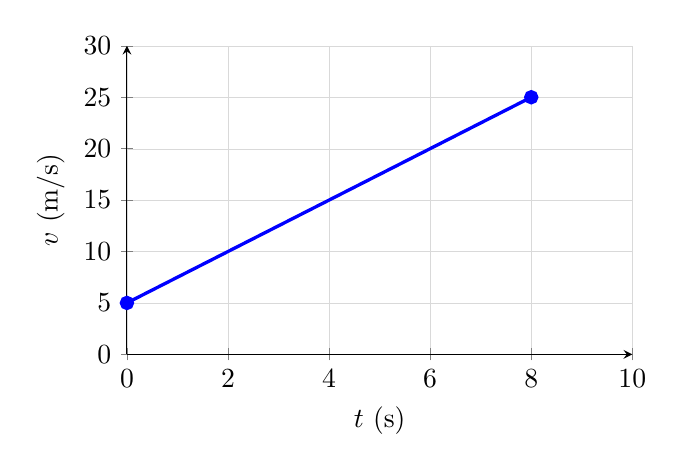
\begin{tikzpicture}
            \begin{axis}[width=8cm, height=5.5cm, grid=both, grid style={line width=.1pt, draw=gray!30},
                axis lines=left, xlabel={\(t\) (s)}, ylabel={\(v\) (m/s)}, xmin=0, xmax=10, ymin=0, ymax=30, xtick={0,2,...,10}, ytick={0,5,...,30}]
                \addplot[very thick, blue, mark=*] coordinates {(0,5) (8,25)};
            \end{axis}
        \end{tikzpicture}
    \end{center}
    \begin{enumerate}[label=\letraminuscula]
        \item Which quantity is on each axis?
        \item What is the velocity at \(t = 0\)? And at \(t = \qty{4}{\s}\)?
        \item Is the velocity increasing or decreasing?
        \item Calculate the slope. Which quantity is it?
    \end{enumerate}
    \begin{solu}
        \begin{enumerate}[label=\alph*)]
            \item \(v\) (m/s) on the vertical axis, \(t\) (s) on the horizontal axis.
            \item At \(t = 0\): \(v = \qty{5}{\mps}\). At \(t = \qty{4}{\s}\): \(v = \qty{15}{\mps}\).
            \item Increasing: the line goes up.
            \item Slope \(= \dfrac{\qty{25}{\mps} - \qty{5}{\mps}}{\qty{8}{\s} - \qty{0}{\s}} = \qty{2.5}{\mpss}\). It is the \textbf{acceleration}.
        \end{enumerate}
    \end{solu}
\end{exercise}

\begin{exercise}
    Draw, on the same axes, the graphs ``\(x\) vs \(t\)'' of two cyclists, using these tables. Who is faster? How do you see it on the graph?
    \begin{center}
        \begin{tabular}{lccccc}
            \toprule
            \(t\) (s) & 0 & 2 & 4 & 6 & 8 \\
            \midrule
            \(x_A\) (m) & 0 & 8 & 16 & 24 & 32 \\
            \(x_B\) (m) & 0 & 12 & 24 & 36 & 48 \\
            \bottomrule
        \end{tabular}
    \end{center}
    \begin{solu}
        Both are straight lines through the origin. Slope of \(A\): \(\dfrac{32}{8} = \qty{4}{\mps}\); slope of \(B\): \(\dfrac{48}{8} = \qty{6}{\mps}\). \(B\) is faster: its line is \textbf{steeper} (it has a bigger slope).
    \end{solu}
\end{exercise}

%----------------------------------------------------------------------------------------

\section*{Summary}

\begin{itemize}
    \item \textbf{Powers of 10}: \(10^{n}\) is a 1 followed by \(n\) zeros; \(10^{-n}\) has the 1 in the \(n\)-th decimal place; \(10^{0} = 1\).
    \item \textbf{Rules}: \(10^{a} \cdot 10^{b} = 10^{a+b}\); \(\dfrac{10^{a}}{10^{b}} = 10^{a-b}\); \(\dfrac{1}{10^{b}} = 10^{-b}\) (a power of 10 changes the sign of its exponent when it crosses the fraction line); \(\left(10^{a}\right)^{b} = 10^{a \cdot b}\).
    \item \textbf{Isolating} a quantity means leaving it alone, in the numerator, on one side of the equation. We do the opposite operation on both sides or, with the shortcut, it goes to the other side with the opposite operation.
    \item If the unknown is in the \textbf{denominator}, we first bring it up multiplying; otherwise we get \(1/x\), not \(x\).
    \item \textbf{Graphs}: ``A vs B'' means A on the vertical axis and B on the horizontal axis. A straight-line graph is described by where it starts, whether it goes up or down, and its \textbf{slope} \(= \Delta(\text{vertical}) / \Delta(\text{horizontal})\).
\end{itemize}



    \part{Chemistry}

%----------------------------------------------------------------------------------------
%	SECTIONING EXAMPLES CHAPTER
%----------------------------------------------------------------------------------------

    %\chapterimage{orange2c.png} % Chapter heading image % --- imagen antigua ---
    \chapterimage{images/portada_cabeceras/cabecera_general} % Cabecera nueva (las de cada unidad van antes de cada \chapter)
    \chapterspaceabove{6.75cm} % Whitespace from the top of the page to the chapter title on chapter pages
    \chapterspacebelow{7.25cm} % Amount of vertical whitespace from the top margin to the start of the text on chapter pages

%------------------------------------------------


    \chapterimage{images/portada_cabeceras/cabecera_Unit1}
    \chapter{Matter and Measurement}
    % Saberes básicos (LOMLOE) asociados a esta unidad
%----------------------------------------------------------------------------------------
% A. Las destrezas científicas básicas
%   - Metodologías de la investigación científica: se introduce el método científico
%     (observación, hipótesis, experimentación, análisis de resultados y conclusiones) como
%     forma de trabajo propia de la física y la química, con ejemplos y un ejercicio de
%     identificación de sus fases en una investigación sencilla.
%   - El lenguaje científico: unidades del Sistema Internacional y sus símbolos: toda la unidad
%     gira en torno al SI (magnitud, unidad, medida), sus múltiplos y submúltiplos, y las reglas
%     de escritura correcta de los símbolos.
%   - Herramientas matemáticas básicas en diferentes escenarios científicos: uso de factores de
%     conversión, reglas de tres y ecuaciones sencillas (d = m/V) para resolver problemas
%     cuantitativos de conversión de unidades y de cálculo de magnitudes.
%   - Diversos entornos y recursos de aprendizaje científico como el laboratorio: manejo de
%     balanzas, probetas, buretas y pipetas; lectura correcta de instrumentos (menisco,
%     sensibilidad, precisión y exactitud de una medida).
%   - Normas de uso de cada espacio, asegurando y protegiendo así la salud propia y comunitaria
%     (identificación del material de laboratorio, normas generales de seguridad y pictogramas
%     de peligrosidad de los productos químicos, SGA/GHS) y el respeto hacia el medio ambiente.
%
% B. La materia
%   - Experimentos relacionados con los sistemas materiales: conocimiento y descripción de sus
%     propiedades (generales/características, cuantitativas/cualitativas, extensivas/intensivas),
%     su clasificación en cuerpos y sistemas materiales, y el uso de la densidad relativa para
%     predecir si un cuerpo flota o se hunde en un líquido.
%
% (Esta unidad no desarrolla contenidos de los bloques C -la energía-, D -la interacción- ni
% E -el cambio-, que se trabajan en unidades posteriores del curso.)
%----------------------------------------------------------------------------------------

\spacing{1.3}
\raggedbottom % pages with large figures end where the text ends (no stretched gaps between boxes)

%\section{Science and the scientific method}
%
%\begin{definition}[Science]
%    A human activity that explains how nature works, in an organised way that can be tested.
%\end{definition}
%
%Scientists answer their questions by following a set of steps called the \negsubro{scientific method}.
%
%\begin{figure}[H]
%    \centering
%    \includegraphics[width=\textwidth]{Unit_1/scientific_method}
%    \caption{The five steps of the scientific method.}
%    \label{fig:u1_scientific_method}
%\end{figure}
%
%\begin{example}
%
%    \begin{enumerate}[label=\numberballmDarkTeal]
%        \item \textbf{Observation}: the plants in a dark corner of the classroom look pale.
%        \item \textbf{Hypothesis}: ``plants need light to stay green''.
%        \item \textbf{Experiment}: identical plants, same water and soil; some in the light, some in the dark.
%        \item \textbf{Analysis}: after two weeks we measure their colour and height.
%        \item \textbf{Conclusion}: plants in the light are green, the others are pale. The hypothesis is accepted.
%    \end{enumerate}
%\end{example}
%
%\begin{impt}
%    In a good experiment we change \textbf{only one variable} (the light) and keep all the others the same (water, soil, temperature\ldots). That way we know exactly what caused the result.
%\end{impt}
%
%\begin{didyouknow}
%    Alexander Fleming discovered penicillin in 1928 thanks to an \emph{observation}: a mould had killed the bacteria in one of his dishes. Asking ``why?'' was the first step of a discovery that has saved millions of lives.
%\end{didyouknow}
%
%\begin{exercise}
%    A group of students wants to find out whether sugar dissolves faster in hot water or in cold water. Identify, in this investigation, the observation, the hypothesis, the experiment and a possible conclusion.
%    \begin{solu}
%        \textbf{Observation}: sometimes sugar seems to dissolve faster than other times. \\
%        \textbf{Hypothesis}: sugar dissolves faster in hot water than in cold water. \\
%        \textbf{Experiment}: dissolve the same amount of sugar in two identical glasses, one with hot water and one with cold water, stirring in the same way, and measure the time it takes to dissolve completely. \\
%        \textbf{Conclusion}: if the sugar dissolves in less time in the hot water, the hypothesis is confirmed.
%    \end{solu}
%\end{exercise}
%
%\begin{exercise}
%    Say which step of the scientific method (observation, hypothesis, experimentation, analysis of results or conclusions) each sentence describes:
%    \begin{enumerate}[label=\letraminuscula]
%        \item ``Plants watered with fertiliser grow taller than plants watered only with water.''
%        \item ``I think that music helps plants grow faster.''
%        \item ``I water ten identical plants with music and ten without, keeping everything else the same, and measure their height every week.''
%        \item ``I notice that the bread in the kitchen goes mouldy faster in summer than in winter.''
%    \end{enumerate}
%    \begin{solu}
%        \begin{enumerate}[label=\alph*)]
%            \item Conclusion (a statement accepted after comparing results).
%            \item Hypothesis (a testable, proposed explanation).
%            \item Experimentation (the procedure designed to test the hypothesis).
%            \item Observation (a fact that raises a question).
%        \end{enumerate}
%    \end{solu}
%\end{exercise}
%
%\begin{exercise}
%    Explain, in your own words, why in a well-designed experiment scientists change only one variable at a time. Give an example of what could go wrong if two variables were changed at once.
%    \begin{solu}
%        If more than one variable changes at the same time, we cannot know which one is responsible for the result. \\
%        For example, if we water some plants with fertiliser \emph{and} give them more light, and they grow taller, we would not know whether it was the fertiliser, the light, or both.
%    \end{solu}
%\end{exercise}

%----------------------------------------------------------------------------------------

\section{Matter and its properties}

\begin{definition}[Matter]
    Everything that has \textbf{mass} and occupies \textbf{space}.
\end{definition}

\begin{figure}[H]
    \centering
    % [FIGURA ORIGINAL] \includegraphics[width=\textwidth]{Unit_1/matter_definition}
    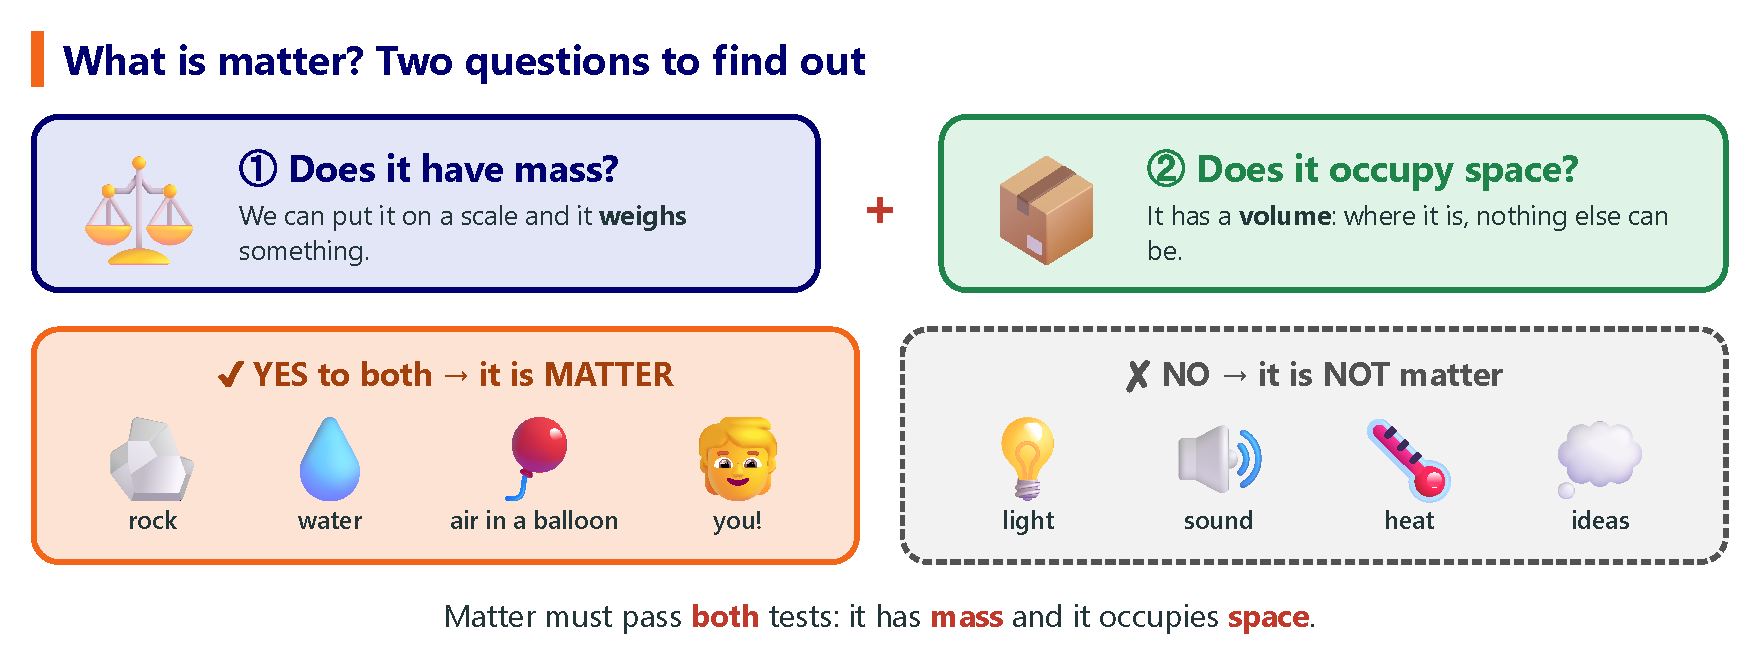
\includegraphics[width=\textwidth]{FigurasSVG/Unit_1_Matter_Measurement/pdf/matter_definition.pdf}
    \caption{To be matter, something must have mass \textbf{and} occupy space. Light, sound, heat or ideas are not matter.}
    \label{fig:u1_matter_definition}
\end{figure}

The bench you sit on, the water you drink and your own body are all matter. Matter is divided into two big groups: \negsubro{bodies} and \negsubro{material systems}.

\begin{definition}[Body]
    A portion of matter that has its \textbf{own shape} and \textbf{defined boundaries}: we can see where it begins and where it ends. For example, a ball, a pencil, a chair or the Moon.
\end{definition}

\begin{definition}[Material system]
    A portion of matter that has \textbf{no shape of its own} and \textbf{no defined boundaries}: it takes the shape of the container that holds it. For example, milk, air, juice or petrol.
\end{definition}

\begin{figure}[H]
    \centering
    % [FIGURA ORIGINAL] \includegraphics[width=\textwidth]{Unit_1/matter_scheme}
    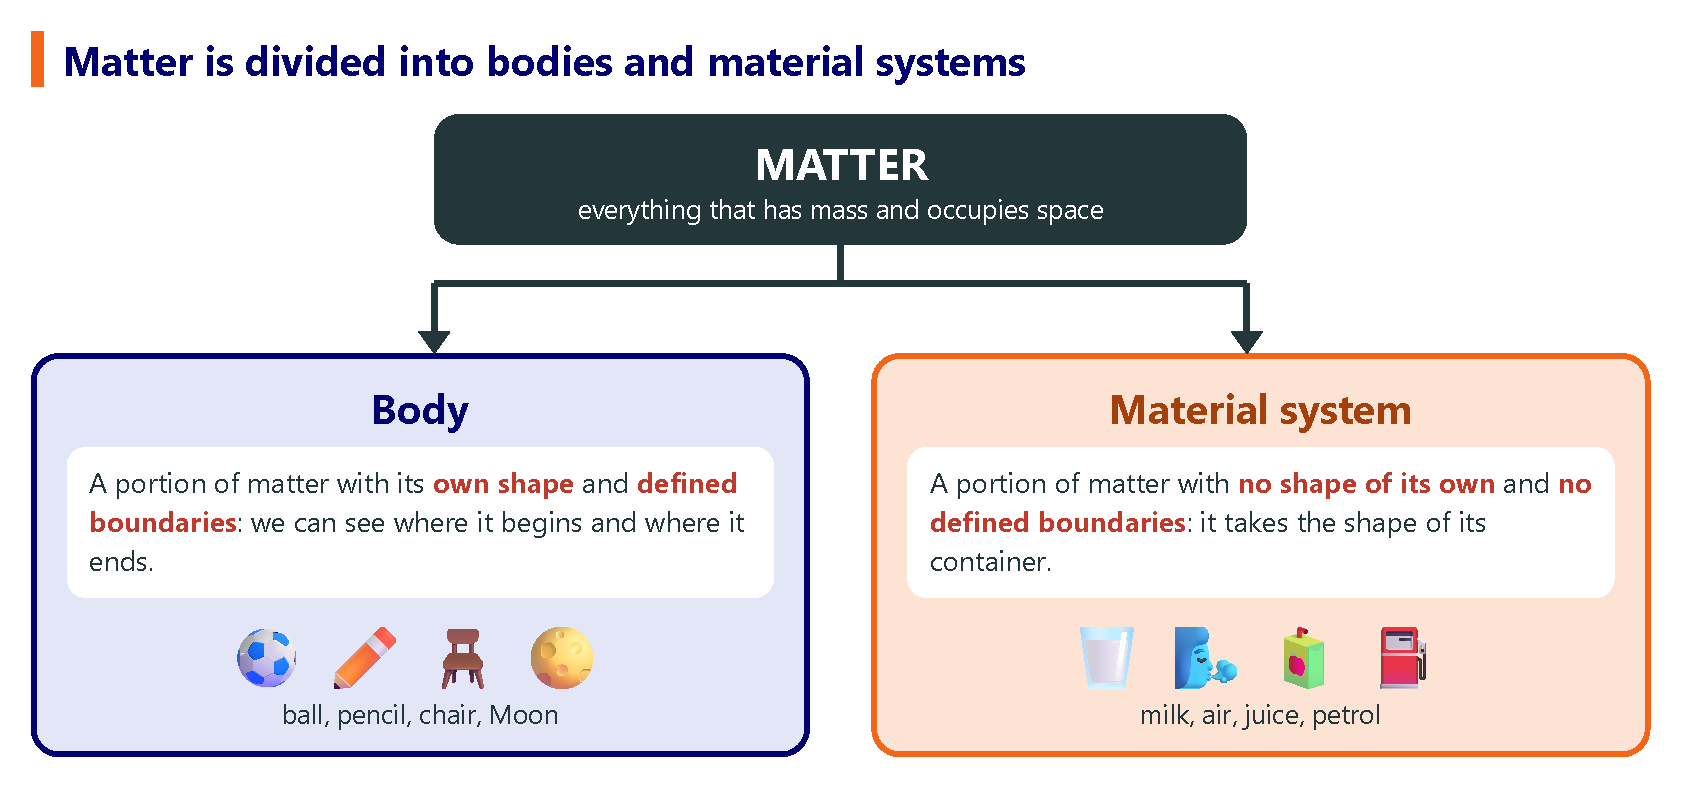
\includegraphics[width=\textwidth]{FigurasSVG/Unit_1_Matter_Measurement/pdf/matter_scheme.pdf}
    \caption{Scheme: matter is divided into bodies and material systems.}
    \label{fig:u1_matter_scheme}
\end{figure}

\begin{figure}[H]
    \centering
    % [FIGURA ORIGINAL] \includegraphics[width=\textwidth]{Unit_1/matter_bodies}
    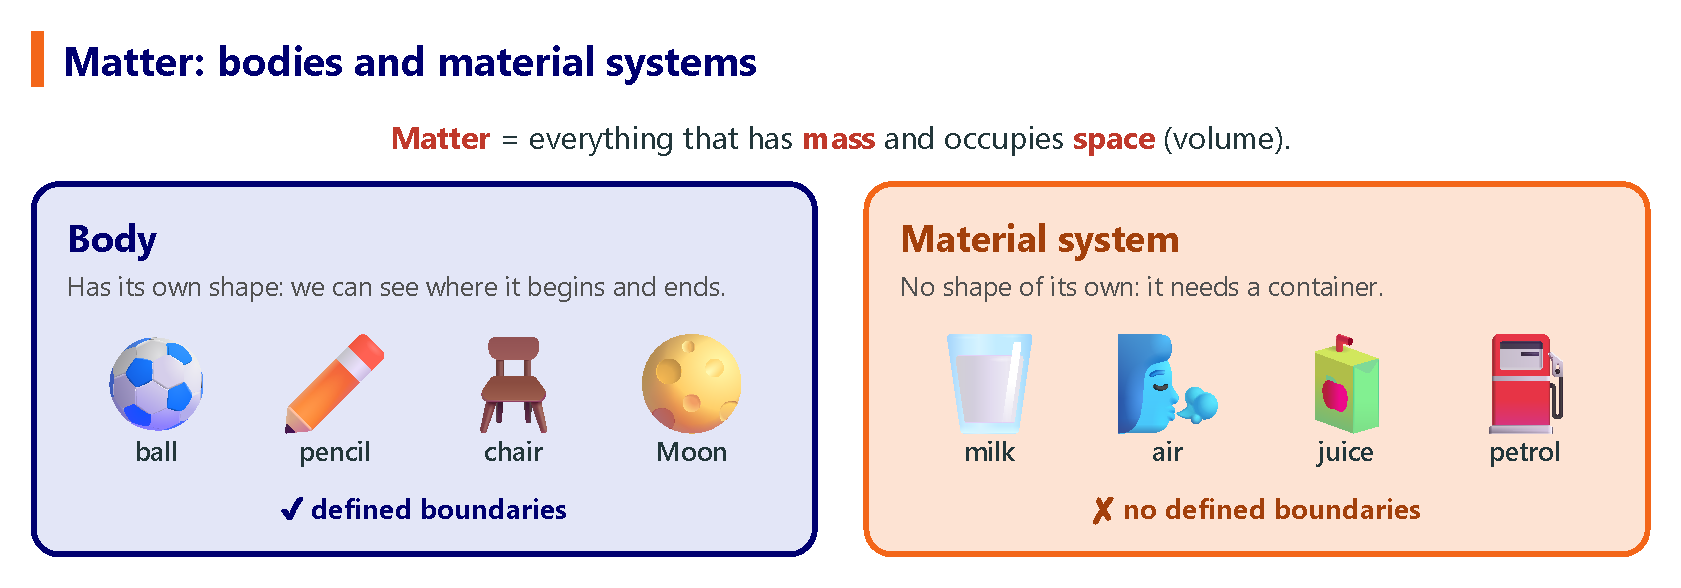
\includegraphics[width=\textwidth]{FigurasSVG/Unit_1_Matter_Measurement/pdf/matter_bodies.pdf}
    \caption{Bodies have their own shape; material systems need a container.}
    \label{fig:u1_matter_bodies}
\end{figure}

\begin{exercise}
    Say whether each of these things is \textbf{matter} or \textbf{not matter}. Remember: to be matter it must have mass \textbf{and} occupy space.
    \begin{enumerate}[label=\letraminuscula]
        \item The air in a room.
        \item Sunlight.
        \item A stone.
        \item The sound of a bell.
        \item A cloud.
        \item The heat from a radiator.
        \item A dream.
        \item The smoke from a fire.
        \item A rainbow.
        \item A drop of oil.
    \end{enumerate}
    \begin{solu}
        \begin{enumerate}[label=\alph*)]
            \item Matter (air has mass and fills the room).
            \item Not matter (light has no mass).
            \item Matter.
            \item Not matter (sound is a vibration that travels through matter, but it is not matter).
            \item Matter (it is made of tiny drops of water).
            \item Not matter (heat is energy).
            \item Not matter (an idea has no mass and does not occupy space).
            \item Matter (it is made of gases and tiny solid particles).
            \item Not matter (it is light).
            \item Matter.
        \end{enumerate}
    \end{solu}
\end{exercise}

\begin{exercise}
    Say whether each of these portions of matter is a \textbf{body} or a \textbf{material system}:
    \begin{enumerate}[label=\letraminuscula]
        \item A coin.
        \item Sea water.
        \item A key.
        \item The oxygen inside a balloon.
        \item Honey.
        \item A pencil.
        \item Olive oil.
        \item A glass marble.
        \item Steam.
        \item A tennis ball.
    \end{enumerate}
    \begin{solu}
        \begin{enumerate}[label=\alph*)]
            \item Body (own shape and defined boundaries).
            \item Material system (it takes the shape of the sea bed or of the container).
            \item Body.
            \item Material system (the gas takes the shape of the balloon).
            \item Material system (it takes the shape of the jar).
            \item Body.
            \item Material system.
            \item Body.
            \item Material system.
            \item Body.
        \end{enumerate}
    \end{solu}
\end{exercise}

\subsection{Physics and chemistry}

Physics and chemistry are the two sciences that study matter and its changes:

\begin{itemize}
    \item \textbf{Physics} studies \negsubro{physical changes}: the substance stays \textbf{the same}.
    \item \textbf{Chemistry} studies \negsubro{chemical changes}: \textbf{new substances} appear.
\end{itemize}

\begin{figure}[H]
    \centering
    % [FIGURA ORIGINAL] \includegraphics[width=\textwidth]{Unit_1/physical_chemical}
    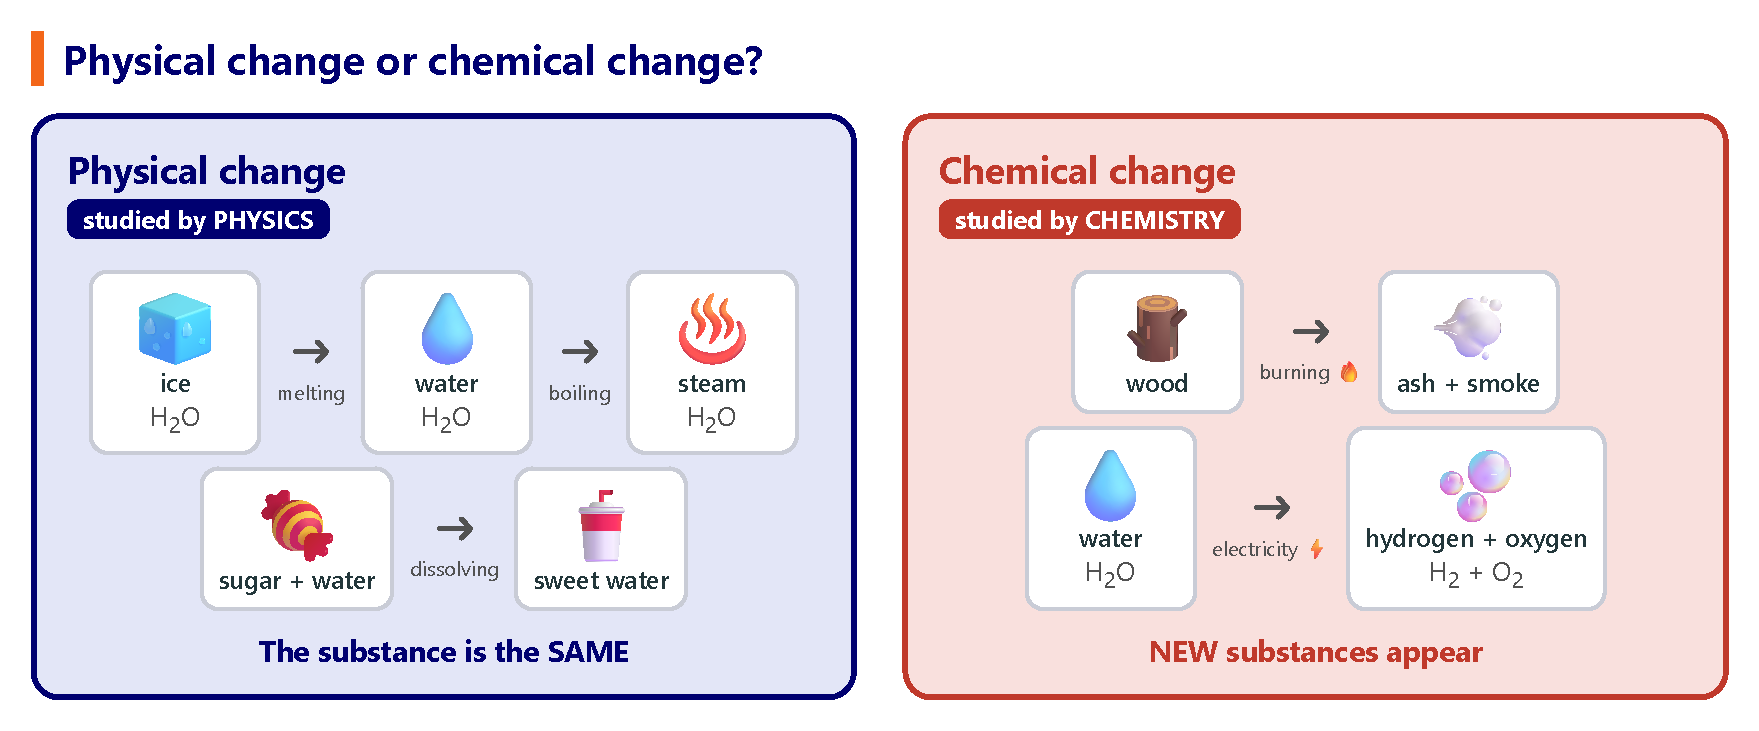
\includegraphics[width=\textwidth]{FigurasSVG/Unit_1_Matter_Measurement/pdf/physical_chemical.pdf}
    \caption{In a physical change the substance is the same; in a chemical change new substances are formed.}
    \label{fig:u1_physical_chemical}
\end{figure}

\begin{impt}
    \textbf{Quick test}: ask yourself ``\emph{Is it still the same substance at the end?}'' If the answer is \textbf{yes} \(\to\) physical change. If \textbf{no} \(\to\) chemical change.
\end{impt}

\begin{exercise}
    Classify these examples as \textbf{physical} or \textbf{chemical} changes:
    \begin{enumerate}[label=\letraminuscula]
        \item Dissolving sugar in water.
        \item Burning wood.
        \item Grinding food.
        \item Moulding a piece of clay.
        \item Melting ice cream.
        \item Frying a steak.
    \end{enumerate}
    \begin{solu}
        \begin{enumerate}[label=\alph*)]
            \item Physical (the sugar is still sugar, only mixed with water).
            \item Chemical (new substances such as ash and smoke appear).
            \item Physical (the food changes shape, not composition).
            \item Physical (only the shape changes).
            \item Physical (change of state, from solid to liquid).
            \item Chemical (the food's composition changes when cooked).
        \end{enumerate}
    \end{solu}
\end{exercise}

\begin{exercise}
    Classify these terms as \textbf{bodies} or \textbf{material systems}:

    Book, phone, aluminium, juice, air, atmosphere, bottle of water, bird, Moon.
    \begin{solu}
        \textbf{Bodies}: book, phone, bottle of water, bird, Moon (they have defined boundaries). \\
        \textbf{Material systems}: aluminium, juice, air, atmosphere (they have no defined boundaries of their own).
    \end{solu}
\end{exercise}

\begin{exercise}
    Say whether physics or chemistry would study each situation, and explain why:
    \begin{enumerate}[label=\letraminuscula]
        \item A metal bar getting longer when it is heated.
        \item A nail rusting after being left outside in the rain.
        \item A ball rolling down a ramp.
        \item Milk turning sour and forming yoghurt.
    \end{enumerate}
    \begin{solu}
        \begin{enumerate}[label=\alph*)]
            \item Physics: the bar is still the same metal, only its size changes.
            \item Chemistry: rust (iron oxide) is a new substance, different from iron.
            \item Physics: the ball's composition does not change, only its position and speed.
            \item Chemistry: yoghurt is a different substance from milk.
        \end{enumerate}
    \end{solu}
\end{exercise}

\subsection{Properties of matter}

\begin{definition}[Property of matter]
    Any aspect of matter that we can observe or measure.
\end{definition}

We classify properties by answering three questions:

\begin{figure}[H]
    \centering
    % [FIGURA ORIGINAL] \includegraphics[width=\textwidth]{Unit_1/properties_map}
    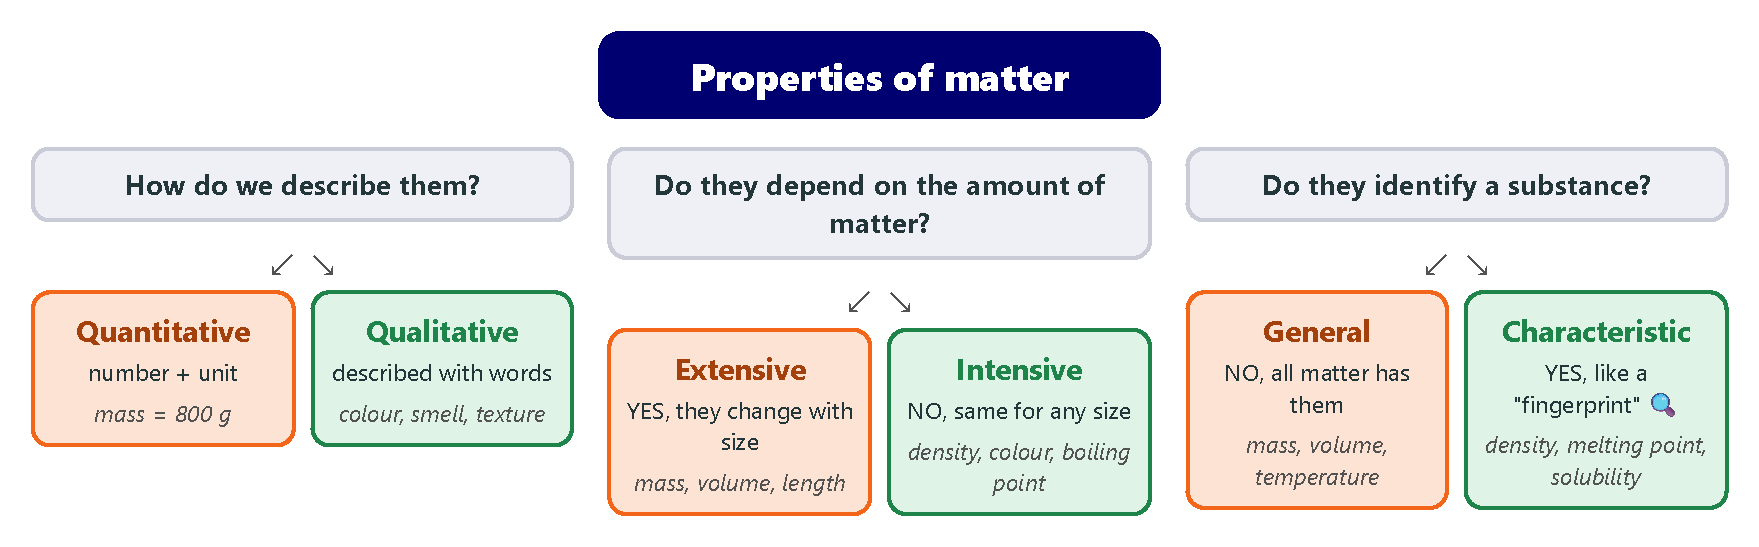
\includegraphics[width=\textwidth]{FigurasSVG/Unit_1_Matter_Measurement/pdf/properties_map.pdf}
    \caption{Three ways of classifying the properties of matter.}
    \label{fig:u1_properties_map}
\end{figure}

These three questions are \textbf{independent}, so we must answer \textbf{all three} for every property. In other words, the \textbf{same property} is, at the same time, of one type in each classification:

\begin{table}[H]
    \centering
    \small
    \renewcommand{\arraystretch}{1.35}
    \begin{tabular}{p{2.4cm}p{3.2cm}p{3.4cm}p{3.4cm}}
        \toprule
        \textbf{Property} & \textbf{How do we describe it?} & \textbf{Does it depend on the amount?} & \textbf{Does it identify a substance?} \\
        \midrule
        Mass & quantitative & extensive & general \\
        Volume & quantitative & extensive & general \\
        Temperature & quantitative & intensive & general \\
        Density & quantitative & intensive & characteristic \\
        Boiling point & quantitative & intensive & characteristic \\
        Colour & qualitative & intensive & characteristic \\
        \bottomrule
    \end{tabular}
    \caption{Each property is classified in the three ways at the same time.}
    \label{tab:u1_three_classifications}
\end{table}

\begin{impt}
    A property is never ``only'' quantitative or ``only'' intensive. For example, \textbf{density} is \textbf{quantitative} (\qty{1.00}{\g\per\mL}), \textbf{intensive} (a drop of water and a swimming pool have the same density) and \textbf{characteristic} (it helps us to identify water).
\end{impt}

\negsubro{Characteristic properties} are the ``fingerprint'' of a substance: they help us to identify it.

\begin{table}[H]
    \centering
    \small
    \renewcommand{\arraystretch}{1.35}
    \begin{tabular}{p{2.2cm}p{3.8cm}p{3.0cm}p{3.2cm}}
        \toprule
        \textbf{Property} & \textbf{What it tells us} & \textbf{Type} & \textbf{Example} \\
        \midrule
        Density & mass in each unit of volume, \(d = m/V\) & quantitative, intensive, characteristic & water: \qty{1.00}{\g\per\mL} \\
        Melting point & temperature at which a solid melts & quantitative, intensive, characteristic & ice: \qty{0}{\celsius} \\
        Boiling point & temperature at which a liquid boils & quantitative, intensive, characteristic & water: \qty{100}{\celsius} \\
        Solubility & how much dissolves in \qty{100}{\g} of water & quantitative, intensive, characteristic & sugar: yes; oil: no \\
        Conductivity & whether it lets heat and electricity pass & quantitative, intensive, characteristic & metals: yes; wood: no \\
        Hardness & resistance to being scratched (scale 1--10) & quantitative, intensive, characteristic & talc: 1; diamond: 10 \\
        \bottomrule
    \end{tabular}
    \caption{Characteristic properties of matter.}
    \label{tab:u1_characteristic}
\end{table}

\begin{exercise}
    Classify each property in the \textbf{three} ways: \textbf{qualitative} or \textbf{quantitative}, \textbf{extensive} or \textbf{intensive}, and \textbf{general} or \textbf{characteristic}.
    \begin{enumerate}[label=\letraminuscula]
        \item Length.
        \item Smell.
        \item Melting point.
        \item Weight.
        \item Hardness.
        \item Shine (lustre) of a metal.
        \item Electrical conductivity.
        \item Taste.
    \end{enumerate}
    \begin{solu}
        \begin{enumerate}[label=\alph*)]
            \item Quantitative, extensive, general.
            \item Qualitative, intensive, characteristic.
            \item Quantitative, intensive, characteristic.
            \item Quantitative, extensive, general.
            \item Quantitative, intensive, characteristic.
            \item Qualitative, intensive, characteristic.
            \item Quantitative, intensive, characteristic.
            \item Qualitative, intensive, characteristic.
        \end{enumerate}
    \end{solu}
\end{exercise}

\begin{exercise}
    Lucía describes her gold ring. Say which property each sentence describes and \textbf{all} its types (each property has one type in each of the three classifications):
    \begin{enumerate}[label=\letraminuscula]
        \item ``The ring has a mass of \qty{6}{\g}.''
        \item ``Gold is yellow and shiny.''
        \item ``Gold melts at \qty{1064}{\celsius}.''
        \item ``The ring occupies \qty{0.31}{\mL}.''
        \item ``The density of gold is \qty{19.3}{\g\per\mL}.''
        \item ``The ring is at \qty{36}{\celsius} because I am wearing it.''
    \end{enumerate}
    \begin{solu}
        \begin{enumerate}[label=\alph*)]
            \item Mass: quantitative, extensive, general.
            \item Colour and shine: qualitative, intensive, characteristic.
            \item Melting point: quantitative, intensive, characteristic.
            \item Volume: quantitative, extensive, general.
            \item Density: quantitative, intensive, characteristic.
            \item Temperature: quantitative, intensive, general.
        \end{enumerate}
    \end{solu}
\end{exercise}



%----------------------------------------------------------------------------------------

\section{Measurement}

% Cancelled unit (in red) for the conversion factors of this section
\providecommand{\cancelunit}[1]{\cancelred{\unit{#1}}}

\begin{definition}[Quantity]
    Any property of matter that can be measured.
\end{definition}

\begin{definition}[Unit]
    A known amount of a quantity, used as a reference to measure that quantity.
\end{definition}

%\begin{definition}[Measure]
%    To measure a quantity, we compare it with a unit to find how many times that unit is contained in it. The result is a \textbf{number} (amount) followed by a \textbf{unit}.
%\end{definition}

To measure a quantity, we compare it with a unit to find how many times that unit is contained in it. The result is a \textbf{number} (amount) followed by a \textbf{unit}.

\begin{example}
    Length of a battery = \qty{5.0}{\cm}. Here, \(\num{5.0}\) is the amount and \(\unit{\cm}\) is the unit.
\end{example}

\subsection{The International System of Units (SI)}

The \negsubro{International System of Units (SI)} sets, for each quantity, one unit, its multiples and its submultiples, plus the rules to write them correctly.

\begin{itemize}
    \item The symbol for a unit is written in lower case, except when it comes from a person's name (J for joule).
    \item The symbol for a multiple/submultiple is written \textbf{before} the unit: km, cL.
    \item Symbols never take a plural ``s'': we write \textbf{8 km}, not 8 kms.
    \item There is always a space between the number and the unit: \textbf{8 m}, not 8m.
\end{itemize}

\begin{didyouknow}
    In 1999 NASA lost the \emph{Mars Climate Orbiter}, a spacecraft worth more than 100 million euros, because one team used SI units (newtons) and another used British units (pounds). The spacecraft got too close to Mars and was destroyed. Units matter!
\end{didyouknow}

\begin{exercise}
    Say whether each of these is written \textbf{correctly} or \textbf{incorrectly} according to the SI rules, and correct the mistakes: ``5 Kg'', ``12 kms'', ``3 J'', ``8m''.
    \begin{solu}
        \begin{itemize}
            \item ``5 Kg'' \(\to\) incorrect, the symbol for kilogram must be lower case: \textbf{5 kg}.
            \item ``12 kms'' \(\to\) incorrect, symbols never take a plural ``s'': \textbf{12 km}.
            \item ``3 J'' \(\to\) correct, J (joule) keeps a capital letter because it comes from a person's name (Joule).
            \item ``8m'' \(\to\) incorrect, there should be a space between the number and the unit: \textbf{8 m}.
        \end{itemize}
    \end{solu}
\end{exercise}

\begin{exercise}
    Explain why the SI is useful for scientists all around the world, even if they speak different languages. Give an example of a problem that could happen if two countries used different units for the same quantity.
    \begin{solu}
        The SI gives one single, agreed set of units and symbols for every quantity, so scientists from different countries can share and understand data without confusion or the need to translate units. \\
        For example, if one team measures a distance in miles and another team reads it as if it were kilometres, they would get a very different (and wrong) value, which could lead to serious errors, such as a spacecraft missing its target.
    \end{solu}
\end{exercise}

%----------------------------------------------------------------------------------------

\subsection{Fundamental and derived quantities}

Not all quantities are equally ``basic''. Some of them are the bricks with which all the others are built.

\begin{definition}[Fundamental quantity]
    A quantity that is defined by itself, without using other quantities. The SI chooses \textbf{seven} fundamental quantities, and each one has its own unit.
\end{definition}

\begin{definition}[Derived quantity]
    A quantity that is obtained by combining fundamental quantities with multiplications or divisions. Its unit is also obtained by combining the units of those fundamental quantities.
\end{definition}

\begin{figure}[H]
    \centering
    % [FIGURA ORIGINAL] \includegraphics[width=\textwidth]{Unit_1/fundamental_derived}
    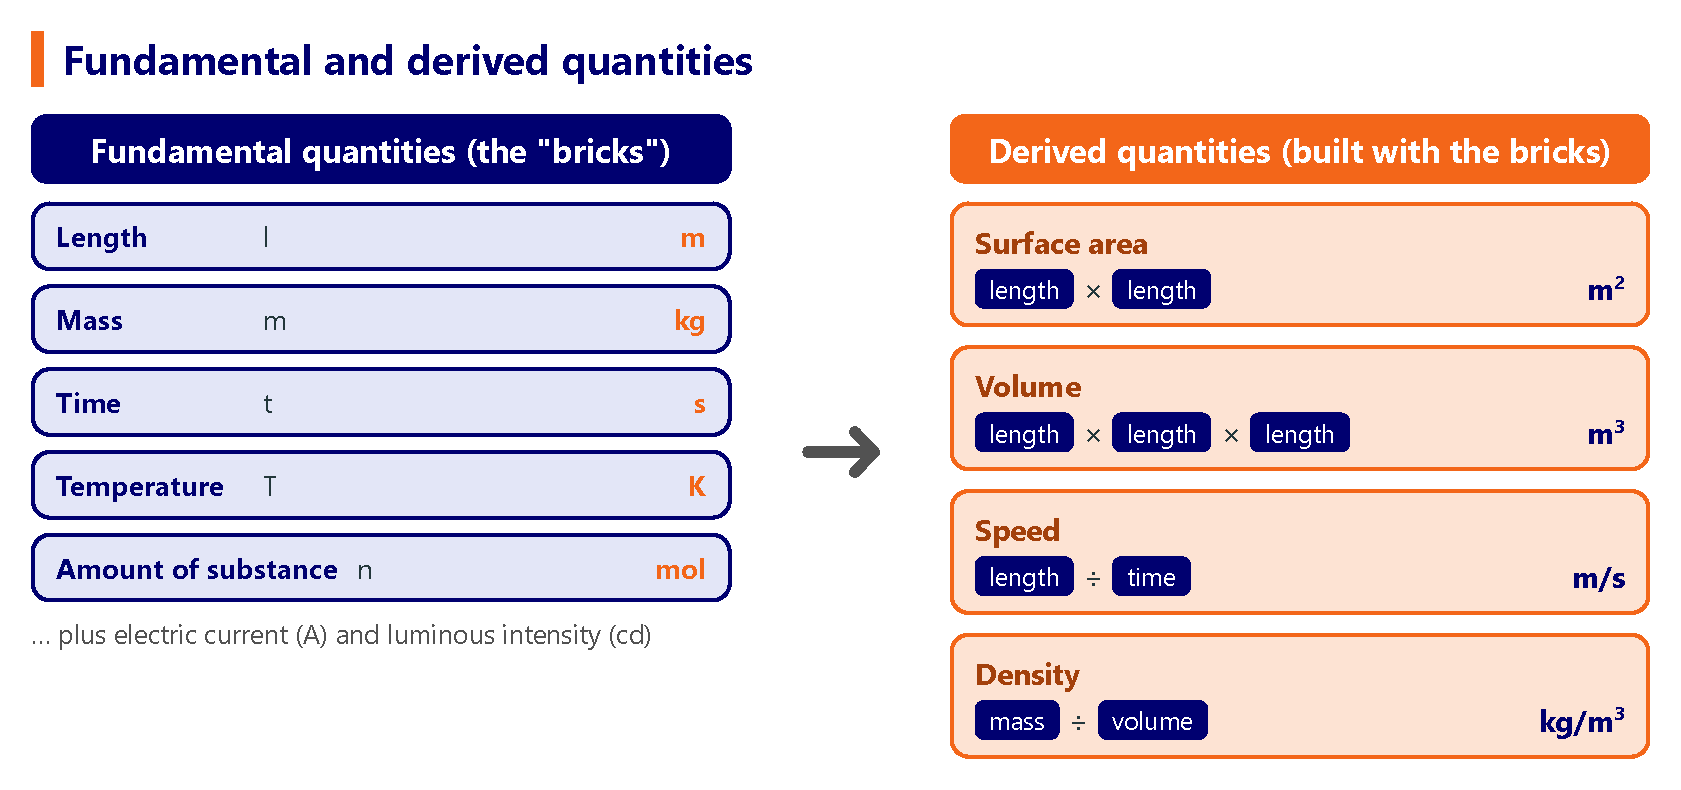
\includegraphics[width=\textwidth]{FigurasSVG/Unit_1_Matter_Measurement/pdf/fundamental_derived.pdf}
    \caption{Fundamental quantities are the ``bricks'' used to build derived quantities.}
    \label{fig:u1_fundamental_derived}
\end{figure}

\begin{table}[H]
    \centering
    \small
    \renewcommand{\arraystretch}{1.35}
    \begin{tabular}{p{2.6cm}cp{3.9cm}p{2.3cm}c}
        \toprule
        \textbf{Quantity} & \textbf{Symbol} & \textbf{Most used units} & \textbf{Unit symbols} & \textbf{SI unit} \\
        \midrule
        Length & \(l\) & kilometre, metre, centimetre, millimetre & \unit{\km}, \unit{\m}, \unit{\cm}, \unit{\mm} & metre (\unit{\m}) \\
        Mass & \(m\) & tonne, kilogram, gram, milligram & \unit{\tonne}, \unit{\kg}, \unit{\g}, \unit{\mg} & kilogram (\unit{\kg}) \\
        Time & \(t\) & day, hour, minute, second & \unit{\day}, \unit{\hour}, \unit{\minute}, \unit{\s} & second (\unit{\s}) \\
        Temperature & \(T\) & degree Celsius, kelvin & \unit{\celsius}, \unit{\K} & kelvin (\unit{\K}) \\
        Amount of substance & \(n\) & mole, millimole & \unit{\mol}, \unit{\milli\mol} & mole (\unit{\mol}) \\
        Electric current & \(I\) & ampere, milliampere & \unit{\A}, \unit{\mA} & ampere (\unit{\A}) \\
        Luminous intensity & \(I_{v}\) & candela & \unit{\candela} & candela (\unit{\candela}) \\
        \bottomrule
    \end{tabular}
    \caption{Fundamental quantities and their most used units.}
    \label{tab:u1_fundamental}
\end{table}

\begin{table}[H]
    \centering
    \small
    \renewcommand{\arraystretch}{1.35}
    \begin{tabular}{p{2.6cm}cp{3.9cm}p{2.3cm}c}
        \toprule
        \textbf{Quantity} & \textbf{Symbol} & \textbf{Most used units} & \textbf{Unit symbols} & \textbf{SI unit} \\
        \midrule
        Surface area \newline (length \(\times\) length) & \(S\) & square kilometre, hectare, square metre, square centimetre & \unit{\square\km}, \unit{\hectare}, \unit{\square\m}, \unit{\square\cm} & \unit{\square\m} \\
        Volume \newline (length\(^3\)) & \(V\) & cubic metre, cubic centimetre, litre, millilitre & \unit{\cubic\m}, \unit{\cubic\cm}, \unit{\litre}, \unit{\mL} & \unit{\cubic\m} \\
        Density \newline (mass \(\div\) volume) & \(d\) & kilogram per cubic metre, gram per millilitre, gram per litre & \unit{\kg\per\cubic\m}, \unit{\g\per\mL}, \unit{\g\per\litre} & \unit{\kg\per\cubic\m} \\
        Speed \newline (length \(\div\) time) & \(v\) & kilometre per hour, metre per second & \unit{\km\per\hour}, \unit{\m\per\s} & \unit{\m\per\s} \\
        Force & \(F\) & newton, kilopond & \unit{\N}, \unit{\kp} & newton (\unit{\N}) \\
        Pressure & \(p\) & pascal, atmosphere, millimetre of mercury & \unit{\Pa}, \unit{\atmospher}, \unit{\mmhg} & pascal (\unit{\Pa}) \\
        Energy & \(E\) & joule, calorie, kilocalorie, kilowatt-hour & \unit{\J}, \unit{\calorie}, \unit{\kilo\calorie}, \unit{\kwh} & joule (\unit{\J}) \\
        \bottomrule
    \end{tabular}
    \caption{Some derived quantities and their most used units.}
    \label{tab:u1_derived}
\end{table}

\begin{impt}
    Notice that the symbol of a \textbf{quantity} is written in \textit{italics} (\(m\), \(V\), \(t\)) and the symbol of a \textbf{unit} in upright letters (\unit{\m}, \unit{\litre}, \unit{\s}). Do not mix up \(m\) (the quantity \emph{mass}) with \unit{\m} (the unit \emph{metre}).
\end{impt}

\begin{exercise}
    Classify each quantity as \textbf{fundamental} or \textbf{derived}, and write its SI unit: mass, speed, time, surface area, temperature, density, length, volume.
    \begin{solu}
        \textbf{Fundamental}: mass (\unit{\kg}), time (\unit{\s}), temperature (\unit{\K}), length (\unit{\m}). \\
        \textbf{Derived}: speed (\unit{\m\per\s}), surface area (\unit{\square\m}), density (\unit{\kg\per\cubic\m}), volume (\unit{\cubic\m}).
    \end{solu}
\end{exercise}

\begin{exercise}
    The SI unit of density is \unit{\kg\per\cubic\m}. Explain, using the fundamental quantities, where this unit comes from.
    \begin{solu}
        Density is mass divided by volume, \(d = m/V\). Mass is measured in \unit{\kg}, and volume is length \(\times\) length \(\times\) length, so it is measured in \(\unit{\m}\cdot\unit{\m}\cdot\unit{\m} = \unit{\cubic\m}\). Dividing both units: \unit{\kg\per\cubic\m}.
    \end{solu}
\end{exercise}

%----------------------------------------------------------------------------------------

\subsection{Multiples and submultiples}

The objects we study can be tiny (a bacterium) or enormous (the Earth). If we always used the base unit, we would have to write numbers full of zeros, which are hard to read and easy to get wrong. To avoid this, the SI adds a \negsubro{prefix} in front of the unit.

\begin{definition}[Multiple and submultiple]
    A \textbf{multiple} is a unit bigger than the base unit (\unit{\km} is \(10^{3}\) times bigger than \unit{\m}). A \textbf{submultiple} is a unit smaller than the base unit (\unit{\mm} is \(10^{3}\) times smaller than \unit{\m}). Each one is named by adding a \textbf{prefix} to the base unit, and each prefix is worth a \textbf{power of 10}.
\end{definition}

\begin{figure}[H]
    \centering
    % [FIGURA ORIGINAL] \includegraphics[width=\textwidth]{Unit_1/prefix_scale}
    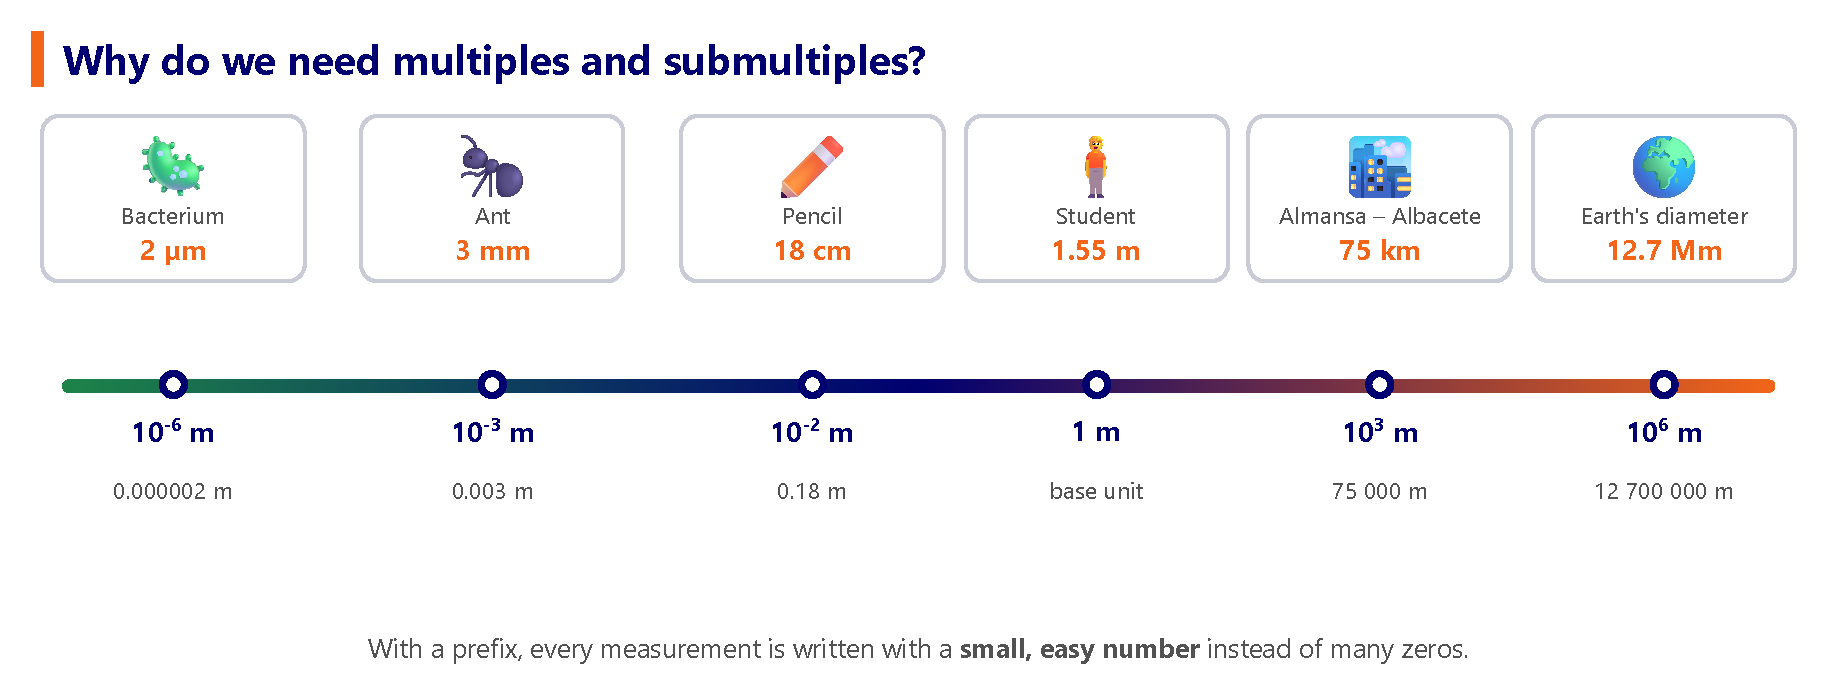
\includegraphics[width=\textwidth]{FigurasSVG/Unit_1_Matter_Measurement/pdf/prefix_scale.pdf}
    \caption{With prefixes, very small and very big lengths are written with simple numbers.}
    \label{fig:u1_prefix_scale}
\end{figure}

\begin{table}[H]
    \centering
    \small
    \renewcommand{\arraystretch}{1.3}
    \begin{tabular}{ccccrl}
        \toprule
         & \textbf{Prefix} & \textbf{Symbol} & \textbf{Power of 10} & \textbf{Decimal value} & \textbf{Example} \\
        \midrule
        \multirow{5}{*}{\rotatebox{90}{\textbf{Multiples}}}
         & giga & G & \(10^{9}\) & \num{1000000000} & \qty{1}{\giga\byte} (memory) \\
         & mega & M & \(10^{6}\) & \num{1000000} & \qty{1}{\mega\m} \\
         & kilo & k & \(10^{3}\) & \num{1000} & \qty{1}{\km}, \qty{1}{\kg} \\
         & hecto & h & \(10^{2}\) & \num{100} & \qty{1}{\hecto\litre} \\
         & deca & da & \(10^{1}\) & \num{10} & \qty{1}{\deca\gram} \\
        \midrule
        \multicolumn{3}{c}{\textbf{Base unit}} & \(10^{0}\) & \num{1} & \unit{\m}, \unit{\g}, \unit{\litre}, \unit{\s} \\
        \midrule
        \multirow{5}{*}{\rotatebox{90}{\textbf{Submultiples}}}
         & deci & d & \(10^{-1}\) & \num{0.1} & \qty{1}{\deci\litre} \\
         & centi & c & \(10^{-2}\) & \num{0.01} & \qty{1}{\cm} \\
         & milli & m & \(10^{-3}\) & \num{0.001} & \qty{1}{\mm}, \qty{1}{\mg} \\
         & micro & \(\upmu\) & \(10^{-6}\) & \num{0.000001} & \qty{1}{\um} (bacterium) \\
         & nano & n & \(10^{-9}\) & \num{0.000000001} & \qty{1}{\nm} (virus) \\
        \bottomrule
    \end{tabular}
    \caption{Multiples and submultiples of the units.}
    \label{tab:u1_prefixes}
\end{table}

\begin{impt}
    \negsubro{Why are multiples and submultiples so important?}
    \begin{itemize}
        \item They let us write any measurement with a \textbf{simple number}: \qty{75}{\km} is much clearer than \qty{75000}{\m}, and \qty{2}{\um} is much clearer than \qty{0.000002}{\m}.
        \item Since every prefix is a \textbf{power of 10}, changing from one to another is very easy: we only move the decimal point.
        \item The same prefixes work for \textbf{all} units: \unit{\km}, \unit{\kg}, \unit{\kilo\litre}, \unit{\kilo\joule}\ldots
    \end{itemize}
\end{impt}

The units of length, mass and capacity can be ordered as a staircase. Each step is worth \textbf{10}, so to know how many times a unit contains another one, we only have to \textbf{count the steps} between them.

\begin{figure}[H]
    \centering
    % [FIGURA ORIGINAL] \includegraphics[width=0.75\textwidth]{Unit_1/prefix_ladder}
    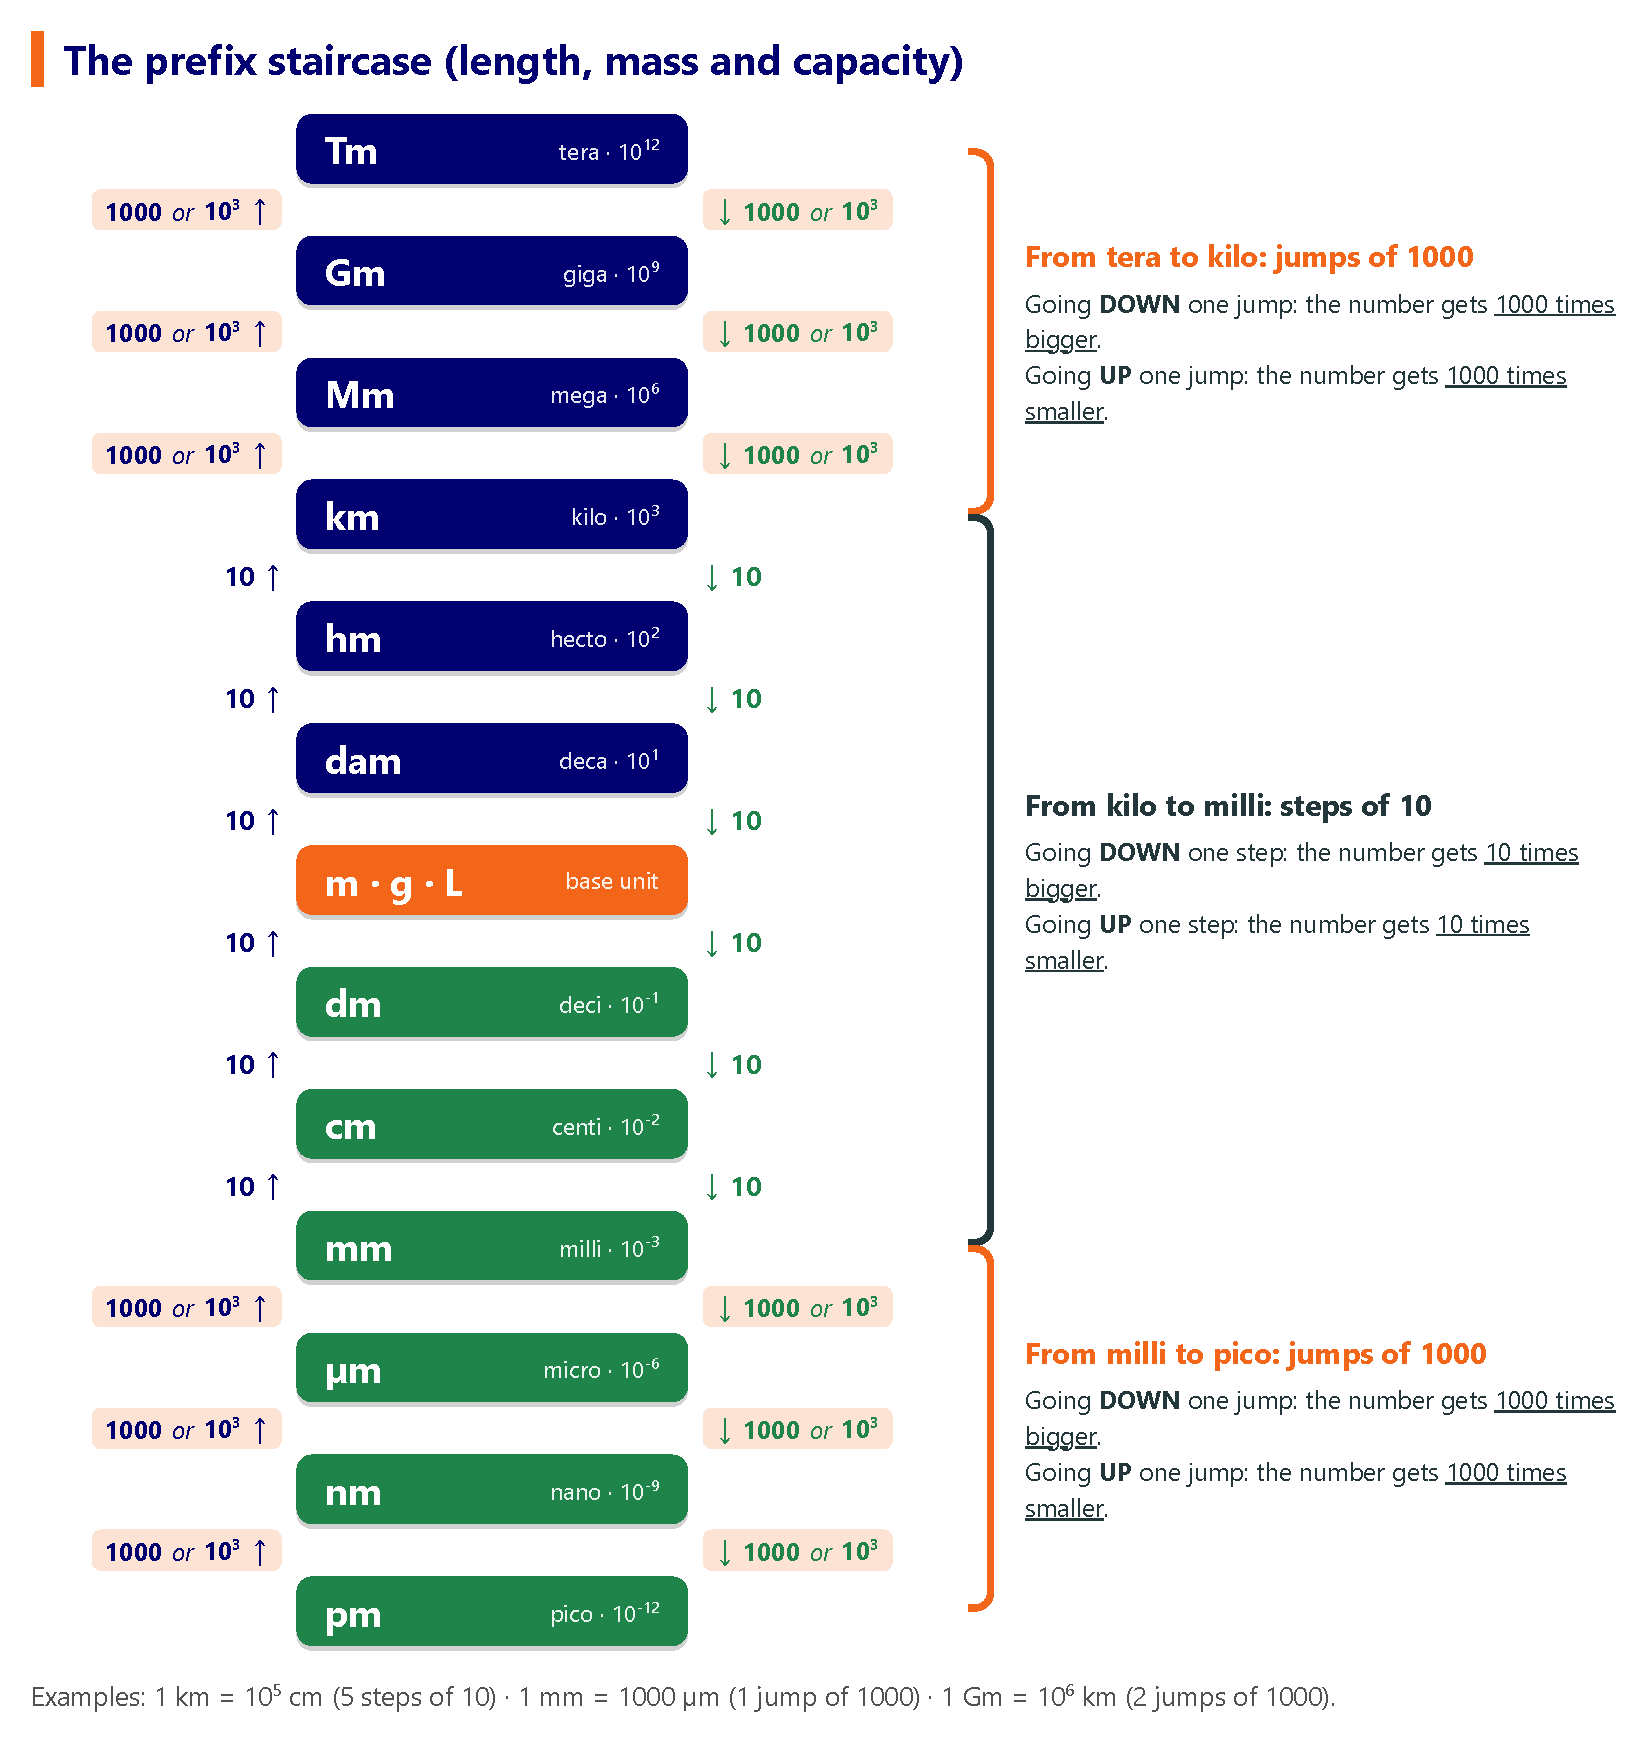
\includegraphics[width=0.75\textwidth]{FigurasSVG/Unit_1_Matter_Measurement/pdf/prefix_ladder.pdf}
    \caption{The prefix staircase: each step is a power of 10.}
    \label{fig:u1_prefix_ladder}
\end{figure}

\begin{example}
    Counting the steps on the staircase:
    \begin{itemize}
        \item From \unit{\km} to \unit{\m} there are 3 steps: \(\qty{1}{\km} = \qty{e3}{\m}\).
        \item From \unit{\m} to \unit{\cm} there are 2 steps: \(\qty{1}{\m} = \qty{e2}{\cm}\).
        \item From \unit{\kg} to \unit{\mg} there are 6 steps: \(\qty{1}{\kg} = \qty{e6}{\mg}\).
        \item From \unit{\deca\litre} to \unit{\centi\litre} there are 3 steps: \(\qty{1}{\deca\litre} = \qty{e3}{\centi\litre}\).
    \end{itemize}
\end{example}

\begin{exercise}
    Write the equivalence between each pair of units, putting the \textbf{1} in front of the bigger unit and using a power of 10: \textbf{a)} \unit{\hecto\m} and \unit{\dm}; \textbf{b)} \unit{\g} and \unit{\mg}; \textbf{c)} \unit{\kilo\litre} and \unit{\mL}; \textbf{d)} \unit{\cm} and \unit{\mm}; \textbf{e)} \unit{\deca\gram} and \unit{\deci\gram}.
    \begin{solu}
        a) \(\qty{1}{\hecto\m} = \qty{e3}{\dm}\); b) \(\qty{1}{\g} = \qty{e3}{\mg}\); c) \(\qty{1}{\kilo\litre} = \qty{e6}{\mL}\); d) \(\qty{1}{\cm} = \qty{e1}{\mm} = \qty{10}{\mm}\); e) \(\qty{1}{\deca\gram} = \qty{e2}{\deci\gram}\).
    \end{solu}
\end{exercise}

\begin{exercise}
    Choose the most suitable unit to express each measurement: the thickness of a coin, the distance from Almansa to Madrid, the mass of a lorry, the mass of a grain of rice, the volume of water in a swimming pool, the volume of a medicine dose.
    \begin{solu}
        Thickness of a coin: \unit{\mm}. Distance Almansa--Madrid: \unit{\km}. Mass of a lorry: \unit{\tonne} or \unit{\kg}. Mass of a grain of rice: \unit{\mg}. Water in a pool: \unit{\cubic\m} or \unit{\kilo\litre}. Medicine dose: \unit{\mL}.
    \end{solu}
\end{exercise}

\begin{impt}
    \negsubro{How to read a unit (very important!)}

    When we look at a unit, we always read it \textbf{from right to left}:
    \begin{enumerate}[label=\numberballmDarkTeal]
        \item First we find the \textbf{symbol of the unit}: it is the \textbf{last} letter (or letters) of the symbol.
        \item Then we identify the \textbf{quantity} that the unit measures: \unit{\m} \(\to\) length, \unit{\g} \(\to\) mass, \unit{\litre} \(\to\) capacity, \unit{\s} \(\to\) time\ldots
        \item Finally, we look at the letter \textbf{in front of the unit}: it is the \textbf{prefix}, and it tells us whether it is a \textbf{multiple} or a \textbf{submultiple}. If there is no letter in front, it is the base unit.
    \end{enumerate}
\end{impt}

\begin{figure}[H]
    \centering
    % [FIGURA ORIGINAL] \includegraphics[width=\textwidth]{Unit_1/read_unit}
    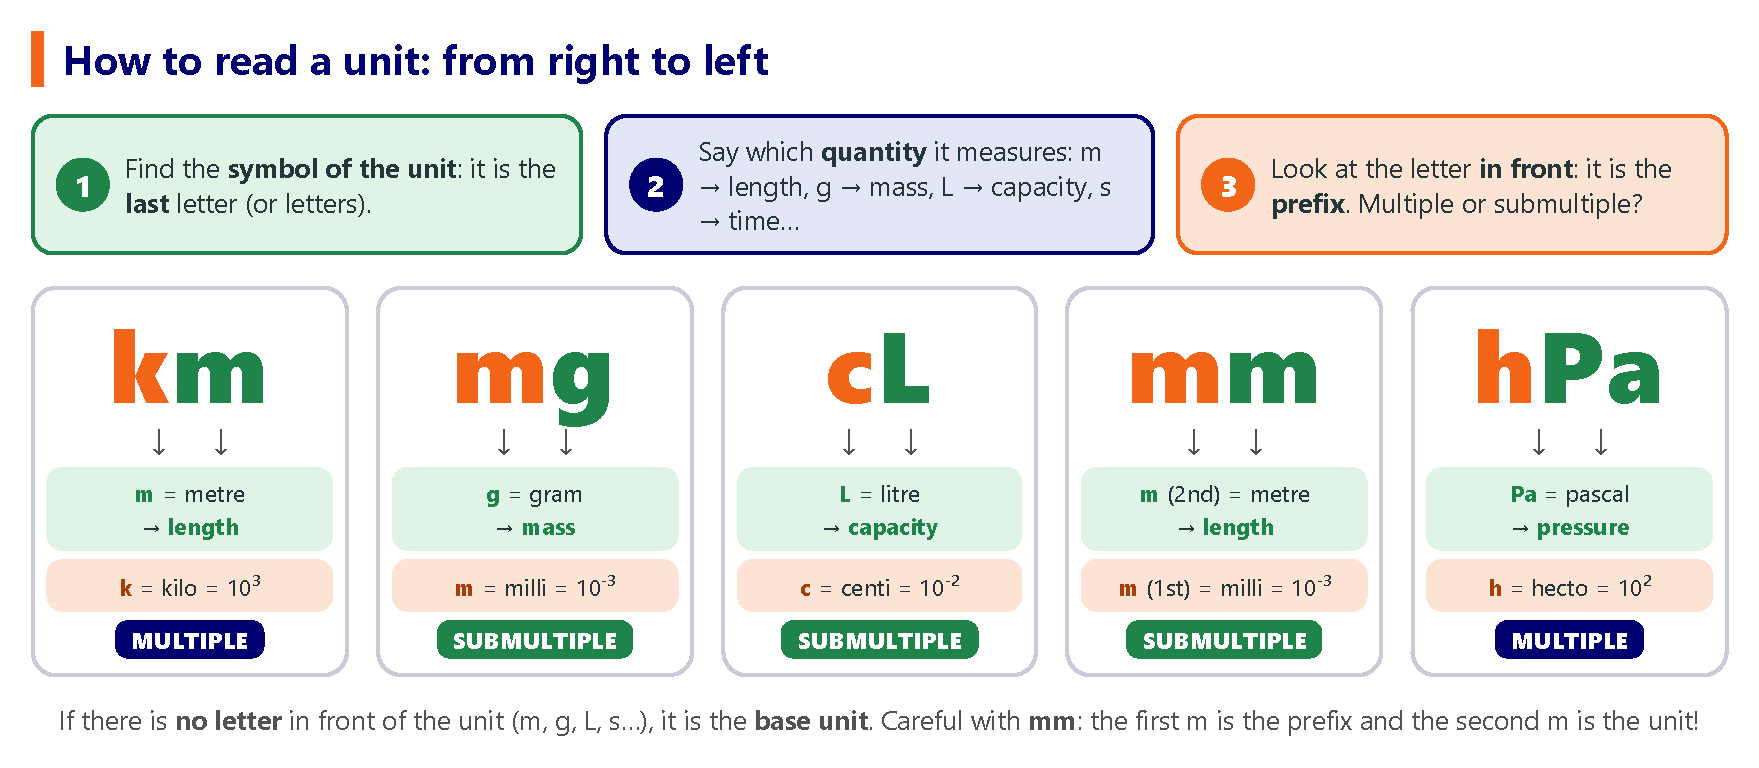
\includegraphics[width=\textwidth]{FigurasSVG/Unit_1_Matter_Measurement/pdf/read_unit.pdf}
    \caption{Reading a unit from right to left: first the unit and its quantity, then the prefix.}
    \label{fig:u1_read_unit}
\end{figure}

\begin{exercise}
    For each unit, say which quantity it measures, which prefix it has and whether it is a multiple or a submultiple: \unit{\kg}, \unit{\mL}, \unit{\cm}, \unit{\hecto\litre}, \unit{\ms}, \unit{\mm}.
    \begin{solu}
        \unit{\kg}: mass, kilo, multiple. \unit{\mL}: capacity, milli, submultiple. \unit{\cm}: length, centi, submultiple. \unit{\hecto\litre}: capacity, hecto, multiple. \unit{\ms}: time, milli, submultiple. \unit{\mm}: length, milli (the first m), submultiple.
    \end{solu}
\end{exercise}

%----------------------------------------------------------------------------------------

\subsection{Changing units: conversion factors}

Very often we need to express a measurement in a different unit: a recipe in grams when our scale uses kilograms, or a speed in \unit{\m\per\s} when the car shows \unit{\km\per\hour}. In this book we will always change units with \negsubro{conversion factors}.

\begin{impt}
    \negsubro{What does ``changing units'' mean?}
    \begin{itemize}
        \item A change of units is a change between \textbf{different units of the same quantity}: \unit{\hour}, \unit{\minute} and \unit{\s} are all units of \textbf{time}, so we can change from one to another.
        \item It is also a change between \textbf{multiples and submultiples} of the same unit: \unit{\km} \(\to\) \unit{\m} \(\to\) \unit{\cm}.
        \item We can \textbf{never} change between units of \textbf{different quantities}: \unit{\km} can never become \unit{\kg}, because length and mass are different quantities.
    \end{itemize}
    The measurement does not change: it is the \textbf{same amount}, only written with a different unit.
\end{impt}

\begin{figure}[H]
    \centering
    % [FIGURA ORIGINAL] \includegraphics[width=\textwidth]{Unit_1/same_quantity}
    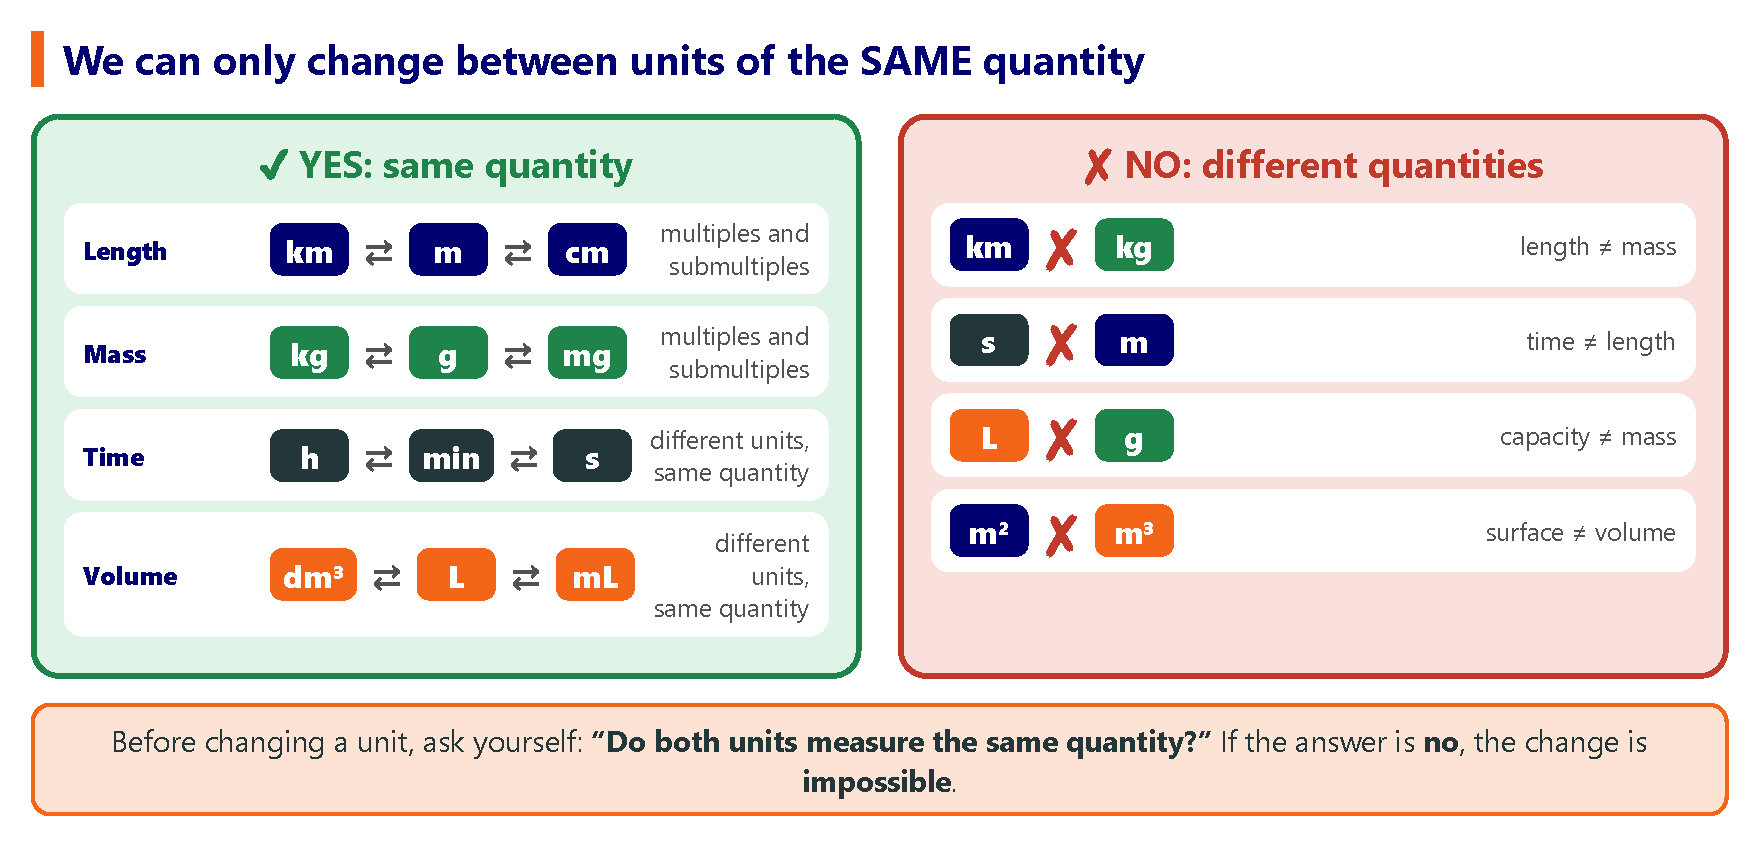
\includegraphics[width=\textwidth]{FigurasSVG/Unit_1_Matter_Measurement/pdf/same_quantity.pdf}
    \caption{We can only change between units that measure the same quantity.}
    \label{fig:u1_same_quantity}
\end{figure}

\begin{definition}[Conversion factor]
    A fraction whose numerator and denominator are the \textbf{same amount}, written in \textbf{different units}. For example,
    \(\dfrac{\qty{e3}{\m}}{\qty{1}{\km}}\) or \(\dfrac{\qty{1}{\km}}{\qty{e3}{\m}}\).
    Since the top and the bottom are equal, a conversion factor is worth exactly \textbf{1}: multiplying by it does not change the quantity, only the unit in which it is written.
\end{definition}

\begin{impt}
    \negsubro{Golden rules for writing conversion factors}
    \begin{enumerate}[label=\numberballmDarkTeal]
        \item In the equivalence between the two units, the \textbf{1} always goes with the \textbf{bigger unit}: \(\qty{1}{\km} = \qty{e3}{\m}\) (never \(\qty{1}{\m} = \qty{e-3}{\km}\)); \(\qty{1}{\hour} = \qty{3600}{\s}\); \(\qty{1}{\atmospher} = \qty{760}{\mmhg}\).
        \item Between multiples and submultiples, and whenever the numbers are very big, we always use \textbf{powers of 10}: \(\qty{1}{\kg} = \qty{e6}{\mg}\) instead of \(\qty{1}{\kg} = \qty{1000000}{\mg}\).
        \item The unit we want to \textbf{remove} goes in the \textbf{denominator}, and the unit we want to \textbf{obtain} goes in the \textbf{numerator}.
    \end{enumerate}
\end{impt}

\begin{figure}[H]
    \centering
    % [FIGURA ORIGINAL] \includegraphics[width=0.95\textwidth]{Unit_1/conversion_factor}
    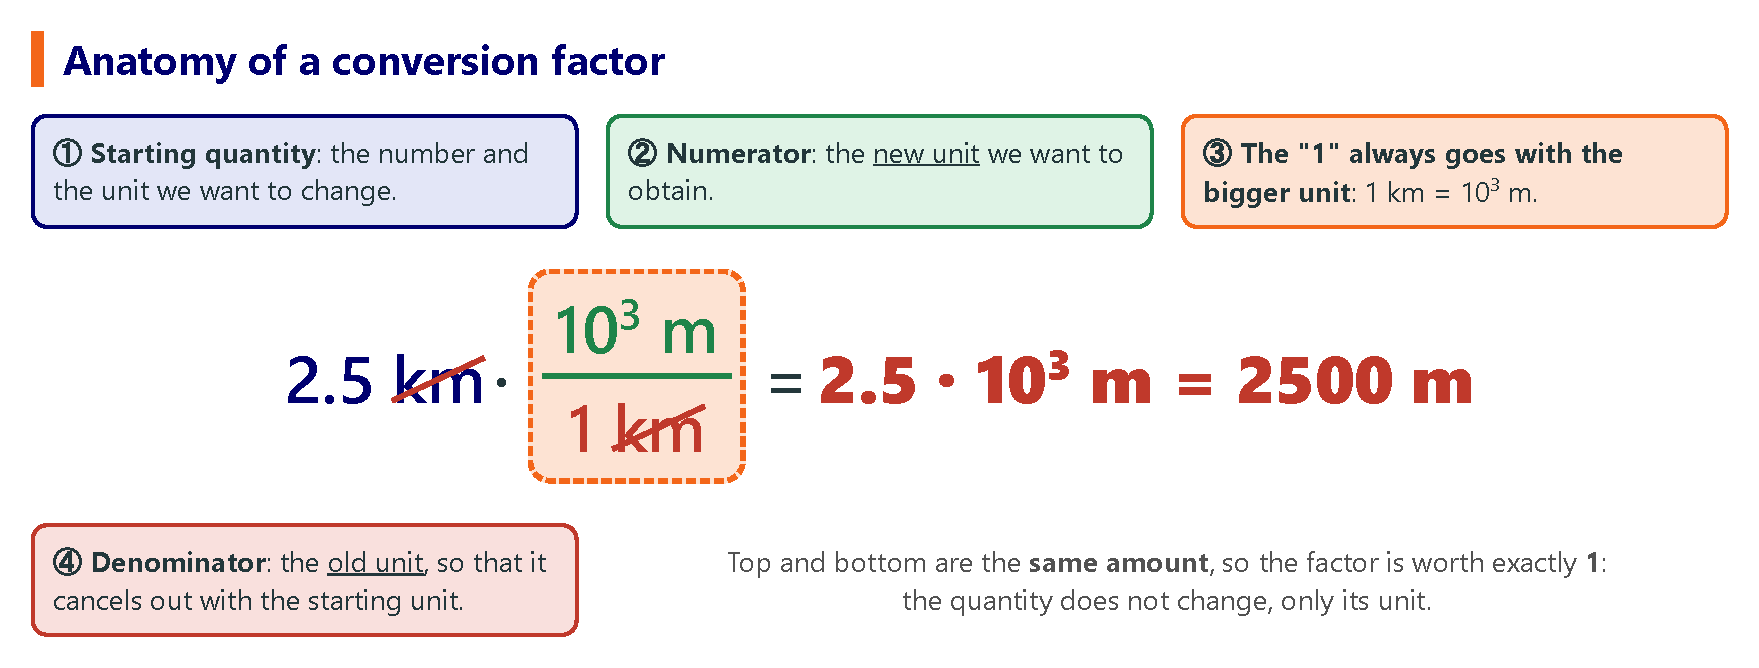
\includegraphics[width=0.95\textwidth]{FigurasSVG/Unit_1_Matter_Measurement/pdf/conversion_factor.pdf}
    \caption{The parts of a conversion factor.}
    \label{fig:u1_conversion_factor}
\end{figure}

\negsubro{Method, step by step}:
\begin{enumerate}[label=\numberballmDarkTeal]
    \item Write the quantity you want to change (number and unit).
    \item Write the \textbf{equivalence} between the initial unit and the final unit, with the 1 in front of the bigger unit and using powers of 10.
    \item Build the \textbf{conversion factor} from the equivalence: the initial unit goes in the denominator, so that it cancels out, and the final unit goes in the numerator.
    \item Multiply, \textbf{cancel} the units that appear above and below, and calculate.
    \item Write the result with its unit (if it has many zeros, leave it as a power of 10).
\end{enumerate}

If there is no direct equivalence between the two units, we can link several conversion factors one after the other, like the links of a chain.

%------------------------------------------------

\subsubsection{Simple units: length, mass and capacity}

\begin{example}
    \textbf{Write \qty{0.8}{\km} in \unit{\dm}.}
    \begin{enumerate}[label=\numberballmDarkTeal]
        \item Quantity: \qty{0.8}{\km}.
        \item Equivalence (4 steps on the staircase, the 1 goes with \unit{\km}): \(\qty{1}{\km} = \qty{e4}{\dm}\).
        \item The unit to remove (\unit{\km}) goes in the denominator.
        \item \(
            \num{0.8}\,\cancelunit{\km} \cdot \dfrac{\qty{e4}{\dm}}{1\,\cancelunit{\km}} = \qty{0.8e4}{\dm}
        \)
        \item \(\textcolor{red}{\qty{8000}{\dm}}\)
    \end{enumerate}
\end{example}

\begin{example}
    \textbf{Write \qty{850}{\deci\gram} in \unit{\hecto\gram}.} \\
    Equivalence (3 steps, the 1 goes with \unit{\hecto\gram}, which is bigger): \(\qty{1}{\hecto\gram} = \qty{e3}{\deci\gram}\).
    \begin{equation*}
        \num{850}\,\cancelunit{\deci\gram} \cdot \dfrac{\qty{1}{\hecto\gram}}{\num{e3}\,\cancelunit{\deci\gram}} = \qty{850e-3}{\hecto\gram} = \textcolor{red}{\qty{0.85}{\hecto\gram}}
    \end{equation*}
\end{example}

\begin{example}
    \textbf{Write \qty{2.5}{\litre} in \unit{\mL}.} \\
    Equivalence: \(\qty{1}{\litre} = \qty{e3}{\mL}\).
    \begin{equation*}
        \num{2.5}\,\cancelunit{\litre} \cdot \dfrac{\qty{e3}{\mL}}{1\,\cancelunit{\litre}} = \qty{2.5e3}{\mL} = \textcolor{red}{\qty{2500}{\mL}}
    \end{equation*}
\end{example}

\begin{exercise}
    Convert these amounts using conversion factors:
    \begin{enumerate}[label=\letraminuscula]
        \item \(\qty{25.8}{\g} \to \unit{\centi\gram}\)
        \item \(\qty{0.05}{\hecto\gram} \to \unit{\deci\gram}\)
        \item \(\qty{3.5}{\deca\gram} \to \unit{\kg}\)
        \item \(\qty{450}{\mg} \to \unit{\kg}\)
        \item \(\qty{1.2}{\km} \to \unit{\cm}\)
        \item \(\qty{330}{\mL} \to \unit{\litre}\)
    \end{enumerate}
    \begin{solu}
        \begin{enumerate}[label=\alph*)]
            \item \(\num{25.8}\,\unit{\g} \cdot \dfrac{\qty{e2}{\centi\gram}}{\qty{1}{\g}} = \qty{2580}{\centi\gram}\)
            \item \(\num{0.05}\,\unit{\hecto\gram} \cdot \dfrac{\qty{e3}{\deci\gram}}{\qty{1}{\hecto\gram}} = \qty{50}{\deci\gram}\)
            \item \(\num{3.5}\,\unit{\deca\gram} \cdot \dfrac{\qty{1}{\kg}}{\qty{e2}{\deca\gram}} = \qty{3.5e-2}{\kg} = \qty{0.035}{\kg}\)
            \item \(\num{450}\,\unit{\mg} \cdot \dfrac{\qty{1}{\kg}}{\qty{e6}{\mg}} = \qty{4.5e-4}{\kg} = \qty{0.00045}{\kg}\)
            \item \(\num{1.2}\,\unit{\km} \cdot \dfrac{\qty{e5}{\cm}}{\qty{1}{\km}} = \qty{1.2e5}{\cm} = \qty{120000}{\cm}\)
            \item \(\num{330}\,\unit{\mL} \cdot \dfrac{\qty{1}{\litre}}{\qty{e3}{\mL}} = \qty{0.33}{\litre}\)
        \end{enumerate}
    \end{solu}
\end{exercise}

\begin{exercise}
    Order these amounts from largest to smallest: \qty{0.015}{\kg}, \qty{2765}{\deci\gram}, \qty{2.54}{\deca\gram}.
    \begin{solu}
        We change all of them to grams: \\
        \(\num{0.015}\,\unit{\kg} \cdot \dfrac{\qty{e3}{\g}}{\qty{1}{\kg}} = \qty{15}{\g}\); \quad
        \(\num{2765}\,\unit{\deci\gram} \cdot \dfrac{\qty{1}{\g}}{\qty{e1}{\deci\gram}} = \qty{276.5}{\g}\); \quad
        \(\num{2.54}\,\unit{\deca\gram} \cdot \dfrac{\qty{e1}{\g}}{\qty{1}{\deca\gram}} = \qty{25.4}{\g}\). \\
        Order: \(\qty{2765}{\deci\gram} > \qty{2.54}{\deca\gram} > \qty{0.015}{\kg}\).
    \end{solu}
\end{exercise}

\begin{exercise}
    A recipe needs \qty{0.75}{\kg} of flour, but the kitchen scale only shows grams. How many grams should be weighed? If a bag contains \qty{2}{\kg} of flour, how many complete recipes can be made with it?
    \begin{solu}
        \(\num{0.75}\,\unit{\kg} \cdot \dfrac{\qty{e3}{\g}}{\qty{1}{\kg}} = \qty{750}{\g}\). \\
        \(\qty{2}{\kg} = \qty{2000}{\g}\); number of recipes \(= 2000 / 750 \approx \num{2.67}\), so \textbf{2 complete recipes} can be made.
    \end{solu}
\end{exercise}

\begin{exercise}
    Convert these amounts using conversion factors:
    \begin{enumerate}[label=\letraminuscula]
        \item \(\qty{500}{\hecto\gram} \to \unit{\g}\)
        \item \(\qty{60}{\cm} \to \unit{\m}\)
        \item \(\qty{2000}{\hecto\m} \to \unit{\deca\m}\)
        \item \(\qty{5.7}{\kg} \to \unit{\g}\)
        \item \(\qty{300}{\dm} \to \unit{\hecto\m}\)
        \item \(\qty{563}{\km} \to \unit{\hecto\m}\)
        \item \(\qty{3}{\dm} \to \unit{\deca\m}\)
        \item \(\qty{7}{\dm} \to \unit{\cm}\)
        \item \(\qty{5}{\giga\m} \to \unit{\nano\m}\)
        \item \(\qty{26}{\micro\m} \to \unit{\km}\)
    \end{enumerate}
    \begin{solu}
        \begin{enumerate}[label=\alph*)]
            \item \(\num{500}\,\unit{\hecto\gram} \cdot \dfrac{\qty{e2}{\g}}{\qty{1}{\hecto\gram}} = \qty{5e4}{\g} = \qty{50000}{\g}\)
            \item \(\num{60}\,\unit{\cm} \cdot \dfrac{\qty{1}{\m}}{\qty{e2}{\cm}} = \qty{0.6}{\m}\)
            \item \(\num{2000}\,\unit{\hecto\m} \cdot \dfrac{\qty{e1}{\deca\m}}{\qty{1}{\hecto\m}} = \qty{2e4}{\deca\m}\)
            \item \(\num{5.7}\,\unit{\kg} \cdot \dfrac{\qty{e3}{\g}}{\qty{1}{\kg}} = \qty{5.7e3}{\g} = \qty{5700}{\g}\)
            \item \(\num{300}\,\unit{\dm} \cdot \dfrac{\qty{1}{\hecto\m}}{\qty{e3}{\dm}} = \qty{0.3}{\hecto\m}\)
            \item \(\num{563}\,\unit{\km} \cdot \dfrac{\qty{e1}{\hecto\m}}{\qty{1}{\km}} = \qty{5630}{\hecto\m}\)
            \item \(\num{3}\,\unit{\dm} \cdot \dfrac{\qty{1}{\deca\m}}{\qty{e2}{\dm}} = \qty{3e-2}{\deca\m} = \qty{0.03}{\deca\m}\)
            \item \(\num{7}\,\unit{\dm} \cdot \dfrac{\qty{e1}{\cm}}{\qty{1}{\dm}} = \qty{70}{\cm}\)
            \item \(\num{5}\,\unit{\giga\m} \cdot \dfrac{\qty{e9}{\m}}{\qty{1}{\giga\m}} \cdot \dfrac{\qty{e9}{\nano\m}}{\qty{1}{\m}} = \qty{5e18}{\nano\m}\)
            \item \(\num{26}\,\unit{\micro\m} \cdot \dfrac{\qty{1}{\m}}{\qty{e6}{\micro\m}} \cdot \dfrac{\qty{1}{\km}}{\qty{e3}{\m}} = \qty{26e-9}{\km} = \qty{2.6e-8}{\km}\)
        \end{enumerate}
    \end{solu}
\end{exercise}

%------------------------------------------------

\subsubsection{Surface area}

\begin{definition}[Surface area]
    A quantity obtained by multiplying two lengths, expressed in the same unit. Its SI unit is the square metre, \unit{\square\metre}.
\end{definition}

\begin{equation*}
    \qty{5.40}{\m} \cdot \qty{6.50}{\m} = \qty{35.10}{\square\metre}
\end{equation*}

A square of \qty{1}{\m} \(\times\) \qty{1}{\m} can be divided into \(10 \times 10 = 100\) small squares of \qty{1}{\dm} \(\times\) \qty{1}{\dm}. So, while \(\qty{1}{\m} = \qty{10}{\dm}\), we have \(\qty{1}{\square\m} = \qty{e2}{\square\dm}\): \textbf{the factor of length is squared}.

\begin{figure}[H]
    \centering
    % [FIGURA ORIGINAL] \includegraphics[width=0.85\textwidth]{Unit_1/square_units}
    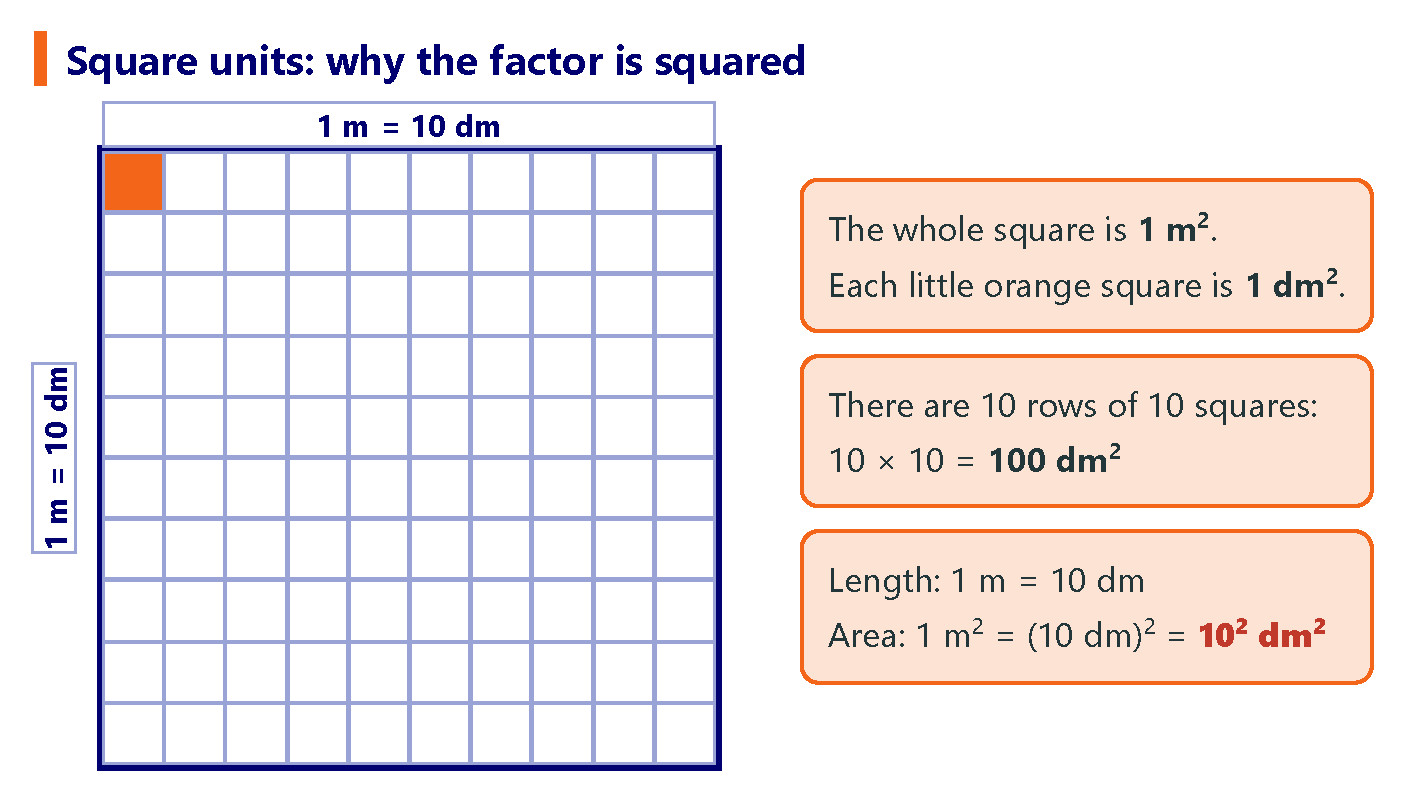
\includegraphics[width=0.85\textwidth]{FigurasSVG/Unit_1_Matter_Measurement/pdf/square_units.pdf}
    \caption{One square metre contains \(10^{2}\) square decimetres.}
    \label{fig:u1_square_units}
\end{figure}

\begin{impt}
    \negsubro{Trick for surface area}: write the conversion factor as if it were a change of \textbf{length} (a simple unit), and then \textbf{raise the whole factor to the power of 2}.
    \begin{equation*}
        \text{Length: } \dfrac{\qty{e2}{\cm}}{\qty{1}{\m}}
        \quad\Longrightarrow\quad
        \text{Surface: } \left(\dfrac{\qty{e2}{\cm}}{\qty{1}{\m}}\right)^{2} = \dfrac{\qty{e4}{\square\cm}}{\qty{1}{\square\m}}
    \end{equation*}
    Each step on the staircase of surface units is therefore worth \(10^{2} = 100\).
\end{impt}

\begin{table}[H]
    \centering
    \small
    \renewcommand{\arraystretch}{1.3}
    \begin{tabular}{cccc}
        \toprule
        \textbf{Unit} & \textbf{Symbol} & \textbf{Equivalence with \unit{\square\m}} & \textbf{Equivalent length} \\
        \midrule
        square kilometre & \unit{\square\km} & \(\qty{1}{\square\km} = \qty{e6}{\square\m}\) & \(\qty{1}{\km} = \qty{e3}{\m}\) \\
        square hectometre (hectare) & \unit{\square\hecto\m} (\unit{\hectare}) & \(\qty{1}{\square\hecto\m} = \qty{e4}{\square\m}\) & \(\qty{1}{\hecto\m} = \qty{e2}{\m}\) \\
        square decametre & \unit{\square\deca\m} & \(\qty{1}{\square\deca\m} = \qty{e2}{\square\m}\) & \(\qty{1}{\deca\m} = \qty{e1}{\m}\) \\
        \midrule
        square metre & \unit{\square\m} & base unit & base unit \\
        \midrule
        square decimetre & \unit{\square\dm} & \(\qty{1}{\square\m} = \qty{e2}{\square\dm}\) & \(\qty{1}{\m} = \qty{e1}{\dm}\) \\
        square centimetre & \unit{\square\cm} & \(\qty{1}{\square\m} = \qty{e4}{\square\cm}\) & \(\qty{1}{\m} = \qty{e2}{\cm}\) \\
        square millimetre & \unit{\square\mm} & \(\qty{1}{\square\m} = \qty{e6}{\square\mm}\) & \(\qty{1}{\m} = \qty{e3}{\mm}\) \\
        \bottomrule
    \end{tabular}
    \caption{Units of surface area.}
    \label{tab:u1_surface_units}
\end{table}

\begin{example}
    \textbf{Write \qty{0.5}{\square\deca\metre} in \unit{\square\dm}.}
    \begin{enumerate}[label=\numberballmDarkTeal]
        \item Simple change (length): \(\qty{1}{\deca\m} = \qty{e2}{\dm}\) \(\to\) factor \(\dfrac{\qty{e2}{\dm}}{\qty{1}{\deca\m}}\).
        \item We square it: \(\left(\dfrac{\qty{e2}{\dm}}{\qty{1}{\deca\m}}\right)^{2} = \dfrac{\qty{e4}{\square\dm}}{\qty{1}{\square\deca\m}}\).
        \item \(
            \num{0.5}\,\cancelunit{\square\deca\m} \cdot \dfrac{\qty{e4}{\square\dm}}{1\,\cancelunit{\square\deca\m}} = \qty{0.5e4}{\square\dm} = \textcolor{red}{\qty{5000}{\square\dm}}
        \)
    \end{enumerate}
\end{example}

\begin{example}
    \textbf{Write \qty{85}{\square\cm} in \unit{\square\m}.} \\
    Simple change: \(\qty{1}{\m} = \qty{e2}{\cm}\). Squaring the factor:
    \begin{equation*}
        \num{85}\,\cancelunit{\square\cm} \cdot \left(\dfrac{\qty{1}{\m}}{\num{e2}\,\cancelunit{\cm}}\right)^{2}
        = \num{85}\,\cancelunit{\square\cm} \cdot \dfrac{\qty{1}{\square\m}}{\num{e4}\,\cancelunit{\square\cm}}
        = \qty{85e-4}{\square\m} = \textcolor{red}{\qty{8.5e-3}{\square\m}}
    \end{equation*}
\end{example}

\begin{exercise}
    Convert these amounts using conversion factors:
    \begin{enumerate}[label=\letraminuscula]
        \item \(\qty{1.25}{\square\m} \to \unit{\square\cm}\)
        \item \(\qty{0.082}{\square\km} \to \unit{\square\dm}\)
        \item \(\qty{1.007}{\square\deca\metre} \to \unit{\square\mm}\)
        \item \(\qty{3500}{\square\mm} \to \unit{\square\dm}\)
    \end{enumerate}
    \begin{solu}
        \begin{enumerate}[label=\alph*)]
            \item \(\num{1.25}\,\unit{\square\m} \cdot \left(\dfrac{\qty{e2}{\cm}}{\qty{1}{\m}}\right)^{2} = \num{1.25}\,\unit{\square\m} \cdot \dfrac{\qty{e4}{\square\cm}}{\qty{1}{\square\m}} = \qty{1.25e4}{\square\cm} = \qty{12500}{\square\cm}\)
            \item \(\num{0.082}\,\unit{\square\km} \cdot \left(\dfrac{\qty{e4}{\dm}}{\qty{1}{\km}}\right)^{2} = \num{0.082}\,\unit{\square\km} \cdot \dfrac{\qty{e8}{\square\dm}}{\qty{1}{\square\km}} = \qty{8.2e6}{\square\dm}\)
            \item \(\num{1.007}\,\unit{\square\deca\m} \cdot \left(\dfrac{\qty{e4}{\mm}}{\qty{1}{\deca\m}}\right)^{2} = \num{1.007}\,\unit{\square\deca\m} \cdot \dfrac{\qty{e8}{\square\mm}}{\qty{1}{\square\deca\m}} = \qty{1.007e8}{\square\mm}\)
            \item \(\num{3500}\,\unit{\square\mm} \cdot \left(\dfrac{\qty{1}{\dm}}{\qty{e2}{\mm}}\right)^{2} = \num{3500}\,\unit{\square\mm} \cdot \dfrac{\qty{1}{\square\dm}}{\qty{e4}{\square\mm}} = \qty{0.35}{\square\dm}\)
        \end{enumerate}
    \end{solu}
\end{exercise}

\begin{exercise}
    A hectare (\unit{\hectare}) is the same as \qty{1}{\square\hecto\m}, that is, \qty{e4}{\square\m}. How many hectares is a football pitch that is \qty{100}{\m} long and \qty{70}{\m} wide?
    \begin{solu}
        Area \(= \qty{100}{\m} \cdot \qty{70}{\m} = \qty{7000}{\square\m}\). \\
        \(\num{7000}\,\unit{\square\m} \cdot \dfrac{\qty{1}{\hectare}}{\qty{e4}{\square\m}} = \qty{0.7}{\hectare}\).
    \end{solu}
\end{exercise}

\begin{exercise}
    A classroom floor measures \qty{8}{\m} by \qty{6}{\m}, and it is going to be covered with square tiles of \qty{400}{\square\cm} each. How many tiles are needed?
    \begin{solu}
        Floor area: \(\qty{8}{\m} \cdot \qty{6}{\m} = \qty{48}{\square\m}\). \\
        \(\num{48}\,\unit{\square\m} \cdot \left(\dfrac{\qty{e2}{\cm}}{\qty{1}{\m}}\right)^{2} = \num{48}\,\unit{\square\m} \cdot \dfrac{\qty{e4}{\square\cm}}{\qty{1}{\square\m}} = \qty{4.8e5}{\square\cm}\). \\
        Number of tiles: \(\num{480000} / \num{400} = \num{1200}\) tiles.
    \end{solu}
\end{exercise}

\begin{exercise}
    Convert these amounts using conversion factors:
    \begin{enumerate}[label=\letraminuscula]
        \item \(\qty{40}{\square\cm} \to \unit{\square\dm}\)
        \item \(\qty{3}{\square\hecto\m} \to \unit{\square\dm}\)
        \item \(\qty{50}{\square\cm} \to \unit{\square\m}\)
        \item \(\qty{0.02}{\square\dm} \to \unit{\square\deca\m}\)
        \item \(\qty{5}{\square\cm} \to \unit{\square\m}\)
        \item \(\qty{300}{\square\hecto\m} \to \unit{\square\dm}\)
        \item \(\qty{653}{\square\cm} \to \unit{\square\m}\)
        \item \(\qty{3}{\square\dm} \to \unit{\square\deca\m}\)
        \item \(\qty{1.5}{\square\hecto\m} \to \unit{\square\mm}\)
        \item \(\qty{5}{\square\giga\m} \to \unit{\square\nano\m}\)
        \item \(\qty{26}{\square\micro\m} \to \unit{\square\km}\)
    \end{enumerate}
    \begin{solu}
        \begin{enumerate}[label=\alph*)]
            \item \(\num{40}\,\unit{\square\cm} \cdot \left(\dfrac{\qty{1}{\dm}}{\qty{e1}{\cm}}\right)^{2} = \num{40}\,\unit{\square\cm} \cdot \dfrac{\qty{1}{\square\dm}}{\qty{e2}{\square\cm}} = \qty{0.4}{\square\dm}\)
            \item \(\num{3}\,\unit{\square\hecto\m} \cdot \left(\dfrac{\qty{e3}{\dm}}{\qty{1}{\hecto\m}}\right)^{2} = \num{3}\,\unit{\square\hecto\m} \cdot \dfrac{\qty{e6}{\square\dm}}{\qty{1}{\square\hecto\m}} = \qty{3e6}{\square\dm}\)
            \item \(\num{50}\,\unit{\square\cm} \cdot \left(\dfrac{\qty{1}{\m}}{\qty{e2}{\cm}}\right)^{2} = \num{50}\,\unit{\square\cm} \cdot \dfrac{\qty{1}{\square\m}}{\qty{e4}{\square\cm}} = \qty{5e-3}{\square\m}\)
            \item \(\num{0.02}\,\unit{\square\dm} \cdot \left(\dfrac{\qty{1}{\deca\m}}{\qty{e2}{\dm}}\right)^{2} = \num{0.02}\,\unit{\square\dm} \cdot \dfrac{\qty{1}{\square\deca\m}}{\qty{e4}{\square\dm}} = \qty{2e-6}{\square\deca\m}\)
            \item \(\num{5}\,\unit{\square\cm} \cdot \left(\dfrac{\qty{1}{\m}}{\qty{e2}{\cm}}\right)^{2} = \num{5}\,\unit{\square\cm} \cdot \dfrac{\qty{1}{\square\m}}{\qty{e4}{\square\cm}} = \qty{5e-4}{\square\m}\)
            \item \(\num{300}\,\unit{\square\hecto\m} \cdot \left(\dfrac{\qty{e3}{\dm}}{\qty{1}{\hecto\m}}\right)^{2} = \num{300}\,\unit{\square\hecto\m} \cdot \dfrac{\qty{e6}{\square\dm}}{\qty{1}{\square\hecto\m}} = \qty{3e8}{\square\dm}\)
            \item \(\num{653}\,\unit{\square\cm} \cdot \left(\dfrac{\qty{1}{\m}}{\qty{e2}{\cm}}\right)^{2} = \num{653}\,\unit{\square\cm} \cdot \dfrac{\qty{1}{\square\m}}{\qty{e4}{\square\cm}} = \qty{6.53e-2}{\square\m} = \qty{0.0653}{\square\m}\)
            \item \(\num{3}\,\unit{\square\dm} \cdot \left(\dfrac{\qty{1}{\deca\m}}{\qty{e2}{\dm}}\right)^{2} = \num{3}\,\unit{\square\dm} \cdot \dfrac{\qty{1}{\square\deca\m}}{\qty{e4}{\square\dm}} = \qty{3e-4}{\square\deca\m}\)
            \item \(\num{1.5}\,\unit{\square\hecto\m} \cdot \left(\dfrac{\qty{e5}{\mm}}{\qty{1}{\hecto\m}}\right)^{2} = \num{1.5}\,\unit{\square\hecto\m} \cdot \dfrac{\qty{e10}{\square\mm}}{\qty{1}{\square\hecto\m}} = \qty{1.5e10}{\square\mm}\)
            \item \(\num{5}\,\unit{\square\giga\m} \cdot \left(\dfrac{\qty{e9}{\m}}{\qty{1}{\giga\m}}\right)^{2} \cdot \left(\dfrac{\qty{e9}{\nano\m}}{\qty{1}{\m}}\right)^{2} = \num{5}\,\unit{\square\giga\m} \cdot \dfrac{\qty{e18}{\square\m}}{\qty{1}{\square\giga\m}} \cdot \dfrac{\qty{e18}{\square\nano\m}}{\qty{1}{\square\m}} = \qty{5e36}{\square\nano\m}\)
            \item \(\num{26}\,\unit{\square\micro\m} \cdot \left(\dfrac{\qty{1}{\m}}{\qty{e6}{\micro\m}}\right)^{2} \cdot \left(\dfrac{\qty{1}{\km}}{\qty{e3}{\m}}\right)^{2} = \num{26}\,\unit{\square\micro\m} \cdot \dfrac{\qty{1}{\square\m}}{\qty{e12}{\square\micro\m}} \cdot \dfrac{\qty{1}{\square\km}}{\qty{e6}{\square\m}} = \qty{26e-18}{\square\km} = \qty{2.6e-17}{\square\km}\)
        \end{enumerate}
    \end{solu}
\end{exercise}

%------------------------------------------------

\subsubsection{Volume}

\begin{definition}[Volume]
    A quantity obtained by multiplying three lengths, expressed in the same unit. Its SI unit is the cubic metre, \unit{\cubic\metre}.
\end{definition}

\begin{equation*}
    \qty{5.40}{\m} \cdot \qty{6.50}{\m} \cdot \qty{3.0}{\m} = \qty{105.3}{\cubic\metre}
\end{equation*}

A cube with sides of \qty{1}{\dm} = \qty{10}{\cm} contains \(10 \times 10 \times 10 = 1000\) small cubes of \qty{1}{\cubic\cm}. So, while \(\qty{1}{\dm} = \qty{10}{\cm}\), we have \(\qty{1}{\cubic\dm} = \qty{e3}{\cubic\cm}\): \textbf{the factor of length is cubed}.

\begin{figure}[H]
    \centering
    % [FIGURA ORIGINAL] \includegraphics[width=0.9\textwidth]{Unit_1/cube_units}
    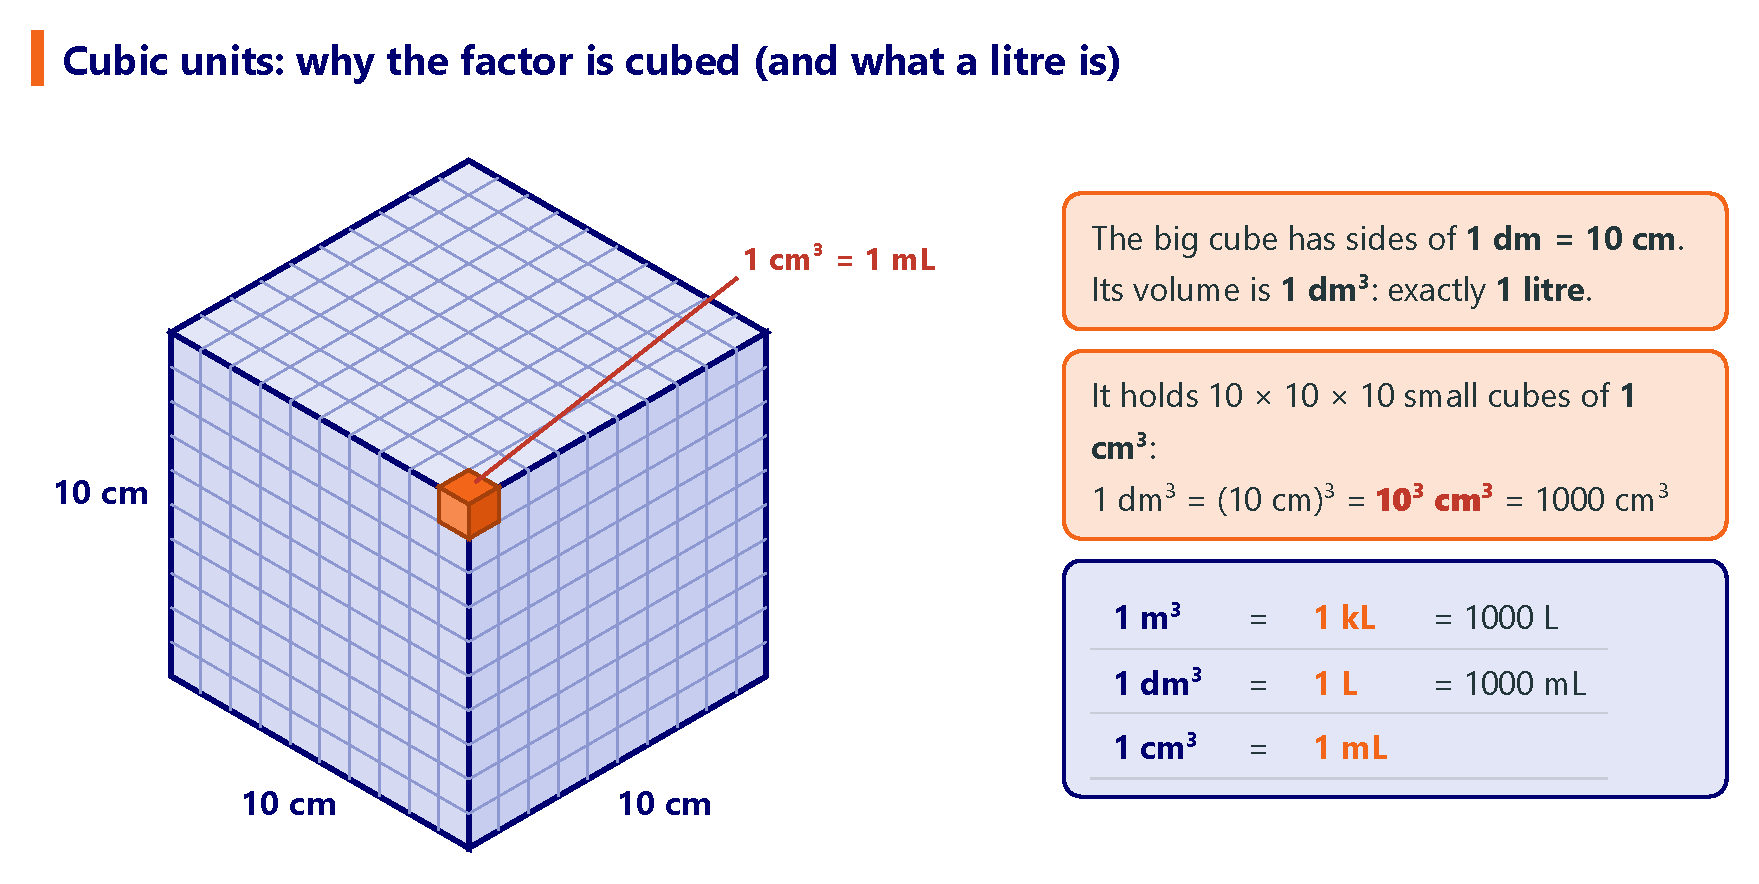
\includegraphics[width=0.9\textwidth]{FigurasSVG/Unit_1_Matter_Measurement/pdf/cube_units.pdf}
    \caption{One cubic decimetre (one litre) contains \(10^{3}\) cubic centimetres (millilitres).}
    \label{fig:u1_cube_units}
\end{figure}

\begin{impt}
    \negsubro{Trick for volume}: we do the same as with surface area, but now we \textbf{raise the factor of length to the power of 3}.
    \begin{equation*}
        \text{Length: } \dfrac{\qty{e2}{\cm}}{\qty{1}{\m}}
        \quad\Longrightarrow\quad
        \text{Volume: } \left(\dfrac{\qty{e2}{\cm}}{\qty{1}{\m}}\right)^{3} = \dfrac{\qty{e6}{\cubic\cm}}{\qty{1}{\cubic\m}}
    \end{equation*}
    Each step on the staircase of volume units is therefore worth \(10^{3} = 1000\).
\end{impt}

\begin{example}
    \textbf{Write \qty{0.5}{\cubic\metre} in \unit{\cubic\mm}.} \\
    Simple change: \(\qty{1}{\m} = \qty{e3}{\mm}\). Cubing the factor:
    \begin{equation*}
        \num{0.5}\,\cancelunit{\cubic\m} \cdot \left(\dfrac{\qty{e3}{\mm}}{1\,\cancelunit{\m}}\right)^{3}
        = \num{0.5}\,\cancelunit{\cubic\m} \cdot \dfrac{\qty{e9}{\cubic\mm}}{1\,\cancelunit{\cubic\m}}
        = \textcolor{red}{\qty{5e8}{\cubic\mm}}
    \end{equation*}
\end{example}

\begin{example}
    \textbf{Write \qty{850}{\cubic\deca\metre} in \unit{\cubic\km}.} \\
    Simple change: \(\qty{1}{\km} = \qty{e2}{\deca\m}\). Cubing the factor:
    \begin{equation*}
        \num{850}\,\cancelunit{\cubic\deca\m} \cdot \left(\dfrac{\qty{1}{\km}}{\num{e2}\,\cancelunit{\deca\m}}\right)^{3}
        = \num{850}\,\cancelunit{\cubic\deca\m} \cdot \dfrac{\qty{1}{\cubic\km}}{\num{e6}\,\cancelunit{\cubic\deca\m}}
        = \qty{850e-6}{\cubic\km} = \textcolor{red}{\qty{8.5e-4}{\cubic\km}}
    \end{equation*}
\end{example}

\begin{exercise}
    Convert these amounts using conversion factors:
    \begin{enumerate}[label=\letraminuscula]
        \item \(\qty{73.357}{\cubic\cm} \to \unit{\cubic\mm}\)
        \item \(\qty{1.0576}{\cubic\deca\metre} \to \unit{\cubic\dm}\)
        \item \(\qty{2500}{\cubic\cm} \to \unit{\cubic\m}\)
    \end{enumerate}
    \begin{solu}
        \begin{enumerate}[label=\alph*)]
            \item \(\num{73.357}\,\unit{\cubic\cm} \cdot \left(\dfrac{\qty{e1}{\mm}}{\qty{1}{\cm}}\right)^{3} = \num{73.357}\,\unit{\cubic\cm} \cdot \dfrac{\qty{e3}{\cubic\mm}}{\qty{1}{\cubic\cm}} = \qty{73357}{\cubic\mm}\)
            \item \(\num{1.0576}\,\unit{\cubic\deca\m} \cdot \left(\dfrac{\qty{e2}{\dm}}{\qty{1}{\deca\m}}\right)^{3} = \num{1.0576}\,\unit{\cubic\deca\m} \cdot \dfrac{\qty{e6}{\cubic\dm}}{\qty{1}{\cubic\deca\m}} = \qty{1.0576e6}{\cubic\dm}\)
            \item \(\num{2500}\,\unit{\cubic\cm} \cdot \left(\dfrac{\qty{1}{\m}}{\qty{e2}{\cm}}\right)^{3} = \num{2500}\,\unit{\cubic\cm} \cdot \dfrac{\qty{1}{\cubic\m}}{\qty{e6}{\cubic\cm}} = \qty{2.5e-3}{\cubic\m}\)
        \end{enumerate}
    \end{solu}
\end{exercise}

\begin{exercise}
    Convert these amounts using conversion factors:
    \begin{enumerate}[label=\letraminuscula]
        \item \(\qty{40}{\cubic\cm} \to \unit{\cubic\dm}\)
        \item \(\qty{e3}{\cubic\km} \to \unit{\cubic\hecto\m}\)
        \item \(\qty{3}{\cubic\deca\m} \to \unit{\cubic\cm}\)
        \item \(\qty{e2}{\cubic\cm} \to \unit{\cubic\dm}\)
        \item \(\qty{7}{\cubic\mm} \to \unit{\cubic\deca\m}\)
        \item \(\qty{2e-2}{\cubic\m} \to \unit{\cubic\mm}\)
        \item \(\qty{5e2}{\cubic\km} \to \unit{\cubic\hecto\m}\)
        \item \(\qty{4.23}{\cubic\deca\m} \to \unit{\cubic\cm}\)
        \item \(\qty{48}{\cubic\cm} \to \unit{\cubic\dm}\)
    \end{enumerate}
    \begin{solu}
        \begin{enumerate}[label=\alph*)]
            \item \(\num{40}\,\unit{\cubic\cm} \cdot \left(\dfrac{\qty{1}{\dm}}{\qty{e1}{\cm}}\right)^{3} = \num{40}\,\unit{\cubic\cm} \cdot \dfrac{\qty{1}{\cubic\dm}}{\qty{e3}{\cubic\cm}} = \qty{4e-2}{\cubic\dm} = \qty{0.04}{\cubic\dm}\)
            \item \(\num{e3}\,\unit{\cubic\km} \cdot \left(\dfrac{\qty{e1}{\hecto\m}}{\qty{1}{\km}}\right)^{3} = \num{e3}\,\unit{\cubic\km} \cdot \dfrac{\qty{e3}{\cubic\hecto\m}}{\qty{1}{\cubic\km}} = \qty{e6}{\cubic\hecto\m}\)
            \item \(\num{3}\,\unit{\cubic\deca\m} \cdot \left(\dfrac{\qty{e3}{\cm}}{\qty{1}{\deca\m}}\right)^{3} = \num{3}\,\unit{\cubic\deca\m} \cdot \dfrac{\qty{e9}{\cubic\cm}}{\qty{1}{\cubic\deca\m}} = \qty{3e9}{\cubic\cm}\)
            \item \(\num{e2}\,\unit{\cubic\cm} \cdot \left(\dfrac{\qty{1}{\dm}}{\qty{e1}{\cm}}\right)^{3} = \num{e2}\,\unit{\cubic\cm} \cdot \dfrac{\qty{1}{\cubic\dm}}{\qty{e3}{\cubic\cm}} = \qty{e-1}{\cubic\dm} = \qty{0.1}{\cubic\dm}\)
            \item \(\num{7}\,\unit{\cubic\mm} \cdot \left(\dfrac{\qty{1}{\deca\m}}{\qty{e4}{\mm}}\right)^{3} = \num{7}\,\unit{\cubic\mm} \cdot \dfrac{\qty{1}{\cubic\deca\m}}{\qty{e12}{\cubic\mm}} = \qty{7e-12}{\cubic\deca\m}\)
            \item \(\num{2e-2}\,\unit{\cubic\m} \cdot \left(\dfrac{\qty{e3}{\mm}}{\qty{1}{\m}}\right)^{3} = \num{2e-2}\,\unit{\cubic\m} \cdot \dfrac{\qty{e9}{\cubic\mm}}{\qty{1}{\cubic\m}} = \qty{2e7}{\cubic\mm}\)
            \item \(\num{5e2}\,\unit{\cubic\km} \cdot \left(\dfrac{\qty{e1}{\hecto\m}}{\qty{1}{\km}}\right)^{3} = \num{5e2}\,\unit{\cubic\km} \cdot \dfrac{\qty{e3}{\cubic\hecto\m}}{\qty{1}{\cubic\km}} = \qty{5e5}{\cubic\hecto\m}\)
            \item \(\num{4.23}\,\unit{\cubic\deca\m} \cdot \left(\dfrac{\qty{e3}{\cm}}{\qty{1}{\deca\m}}\right)^{3} = \num{4.23}\,\unit{\cubic\deca\m} \cdot \dfrac{\qty{e9}{\cubic\cm}}{\qty{1}{\cubic\deca\m}} = \qty{4.23e9}{\cubic\cm}\)
            \item \(\num{48}\,\unit{\cubic\cm} \cdot \left(\dfrac{\qty{1}{\dm}}{\qty{e1}{\cm}}\right)^{3} = \num{48}\,\unit{\cubic\cm} \cdot \dfrac{\qty{1}{\cubic\dm}}{\qty{e3}{\cubic\cm}} = \qty{4.8e-2}{\cubic\dm} = \qty{0.048}{\cubic\dm}\)
        \end{enumerate}
    \end{solu}
\end{exercise}

%------------------------------------------------

\subsubsection{Volume and capacity: cubic units and litres}

We use \textbf{volume} for the space occupied by a body and \textbf{capacity} for what a container can hold, but they are the same quantity, so their units are related. The three key equivalences are:

\begin{table}[H]
    \centering
    \renewcommand{\arraystretch}{1.4}
    \begin{tabular}{ccc}
        \toprule
        \textbf{Volume} & & \textbf{Capacity} \\
        \midrule
        \qty{1}{\cubic\m} & = & \qty{1}{\kilo\litre} \\
        \qty{1}{\cubic\dm} & = & \qty{1}{\litre} \\
        \qty{1}{\cubic\cm} & = & \qty{1}{\mL} \\
        \bottomrule
    \end{tabular}
    \caption{Equivalences between volume and capacity units.}
    \label{tab:u1_volume_capacity}
\end{table}

\begin{impt}
    To change between cubic units and litres:
    \begin{enumerate}[label=\numberballmDarkTeal]
        \item Use the conversion factors of volume (cubed) or of capacity (simple) to reach one of the three ``partner'' units: \unit{\cubic\m}--\unit{\kilo\litre}, \unit{\cubic\dm}--\unit{\litre} or \unit{\cubic\cm}--\unit{\mL}.
        \item Jump from volume to capacity (or the other way round) with a factor such as \(\dfrac{\qty{1}{\litre}}{\qty{1}{\cubic\dm}}\), which is worth 1.
    \end{enumerate}
\end{impt}

\begin{example}
    \textbf{Write \qty{2.5}{\cubic\m} in litres.}
    \begin{equation*}
        \num{2.5}\,\cancelunit{\cubic\m} \cdot \dfrac{\qty{1}{\kilo\litre}}{1\,\cancelunit{\cubic\m}} \cdot \dfrac{\qty{e3}{\litre}}{1\,\cancelunit{\kilo\litre}} = \textcolor{red}{\qty{2.5e3}{\litre}} = \qty{2500}{\litre}
    \end{equation*}
\end{example}

\begin{example}
    \textbf{A soft drink can contains \qty{33}{\centi\litre}. Write it in \unit{\cubic\cm}.}
    \begin{equation*}
        \num{33}\,\cancelunit{\centi\litre} \cdot \dfrac{\num{e1}\,\cancelunit{\mL}}{1\,\cancelunit{\centi\litre}} \cdot \dfrac{\qty{1}{\cubic\cm}}{1\,\cancelunit{\mL}} = \textcolor{red}{\qty{330}{\cubic\cm}}
    \end{equation*}
\end{example}

\begin{example}
    \textbf{Write \qty{750}{\mL} in \unit{\cubic\m}.}
    \begin{equation*}
        \num{750}\,\cancelunit{\mL} \cdot \dfrac{1\,\cancelunit{\cubic\cm}}{1\,\cancelunit{\mL}} \cdot \left(\dfrac{\qty{1}{\m}}{\num{e2}\,\cancelunit{\cm}}\right)^{3}
        = \num{750}\,\cancelunit{\cubic\cm} \cdot \dfrac{\qty{1}{\cubic\m}}{\num{e6}\,\cancelunit{\cubic\cm}} = \textcolor{red}{\qty{7.5e-4}{\cubic\m}}
    \end{equation*}
\end{example}

\begin{exercise}
    An Olympic-size swimming pool contains 2.5 million litres of water (\qty{2.5e6}{\litre}). Write it in \unit{\cubic\metre}.
    \begin{solu}
        \(\num{2.5e6}\,\unit{\litre} \cdot \dfrac{\qty{1}{\cubic\dm}}{\qty{1}{\litre}} \cdot \left(\dfrac{\qty{1}{\m}}{\qty{e1}{\dm}}\right)^{3} = \num{2.5e6}\,\unit{\cubic\dm} \cdot \dfrac{\qty{1}{\cubic\m}}{\qty{e3}{\cubic\dm}} = \qty{2.5e3}{\cubic\m} = \qty{2500}{\cubic\m}\).
    \end{solu}
\end{exercise}

\begin{exercise}
    Convert: \textbf{a)} \qty{1.5}{\litre} \(\to\) \unit{\cubic\cm}; \textbf{b)} \qty{40}{\cubic\cm} \(\to\) \unit{\centi\litre}; \textbf{c)} \qty{0.2}{\cubic\m} \(\to\) \unit{\litre}; \textbf{d)} \qty{5}{\mL} \(\to\) \unit{\cubic\dm}.
    \begin{solu}
        a) \(\num{1.5}\,\unit{\litre} \cdot \dfrac{\qty{e3}{\mL}}{\qty{1}{\litre}} \cdot \dfrac{\qty{1}{\cubic\cm}}{\qty{1}{\mL}} = \qty{1500}{\cubic\cm}\) \\
        b) \(\num{40}\,\unit{\cubic\cm} \cdot \dfrac{\qty{1}{\mL}}{\qty{1}{\cubic\cm}} \cdot \dfrac{\qty{1}{\centi\litre}}{\qty{e1}{\mL}} = \qty{4}{\centi\litre}\) \\
        c) \(\num{0.2}\,\unit{\cubic\m} \cdot \dfrac{\qty{1}{\kilo\litre}}{\qty{1}{\cubic\m}} \cdot \dfrac{\qty{e3}{\litre}}{\qty{1}{\kilo\litre}} = \qty{200}{\litre}\) \\
        d) \(\num{5}\,\unit{\mL} \cdot \dfrac{\qty{1}{\litre}}{\qty{e3}{\mL}} \cdot \dfrac{\qty{1}{\cubic\dm}}{\qty{1}{\litre}} = \qty{5e-3}{\cubic\dm}\)
    \end{solu}
\end{exercise}

\begin{exercise}
    A fish tank is a rectangular prism \qty{50}{\cm} long, \qty{30}{\cm} wide and \qty{40}{\cm} high.
    \begin{enumerate}[label=\letraminuscula]
        \item Calculate its volume in \unit{\cubic\cm}.
        \item How many litres of water are needed to fill it completely?
    \end{enumerate}
    \begin{solu}
        \begin{enumerate}[label=\alph*)]
            \item \(V = \qty{50}{\cm} \cdot \qty{30}{\cm} \cdot \qty{40}{\cm} = \qty{60000}{\cubic\cm} = \qty{6e4}{\cubic\cm}\).
            \item \(\num{6e4}\,\unit{\cubic\cm} \cdot \dfrac{\qty{1}{\mL}}{\qty{1}{\cubic\cm}} \cdot \dfrac{\qty{1}{\litre}}{\qty{e3}{\mL}} = \qty{60}{\litre}\).
        \end{enumerate}
    \end{solu}
\end{exercise}

\begin{exercise}
    Convert these amounts using conversion factors:
    \begin{enumerate}[label=\letraminuscula]
        \item \(\qty{0.02}{\cubic\deca\m} \to \unit{\mL}\)
        \item \(\qty{100}{\mL} \to \unit{\cubic\m}\)
        \item \(\qty{300}{\litre} \to \unit{\cubic\deca\m}\)
    \end{enumerate}
    \begin{solu}
        \begin{enumerate}[label=\alph*)]
            \item \(\num{0.02}\,\unit{\cubic\deca\m} \cdot \left(\dfrac{\qty{e3}{\cm}}{\qty{1}{\deca\m}}\right)^{3} \cdot \dfrac{\qty{1}{\mL}}{\qty{1}{\cubic\cm}} = \num{0.02}\,\unit{\cubic\deca\m} \cdot \dfrac{\qty{e9}{\cubic\cm}}{\qty{1}{\cubic\deca\m}} \cdot \dfrac{\qty{1}{\mL}}{\qty{1}{\cubic\cm}} = \qty{2e7}{\mL}\)
            \item \(\num{100}\,\unit{\mL} \cdot \dfrac{\qty{1}{\cubic\cm}}{\qty{1}{\mL}} \cdot \left(\dfrac{\qty{1}{\m}}{\qty{e2}{\cm}}\right)^{3} = \num{100}\,\unit{\cubic\cm} \cdot \dfrac{\qty{1}{\cubic\m}}{\qty{e6}{\cubic\cm}} = \qty{e-4}{\cubic\m}\)
            \item \(\num{300}\,\unit{\litre} \cdot \dfrac{\qty{1}{\cubic\dm}}{\qty{1}{\litre}} \cdot \left(\dfrac{\qty{1}{\deca\m}}{\qty{e2}{\dm}}\right)^{3} = \num{300}\,\unit{\cubic\dm} \cdot \dfrac{\qty{1}{\cubic\deca\m}}{\qty{e6}{\cubic\dm}} = \qty{3e-4}{\cubic\deca\m}\)
        \end{enumerate}
    \end{solu}
\end{exercise}

%------------------------------------------------

\subsubsection{Time}

In the SI, time is measured in \textbf{seconds} (\unit{\s}). For longer times we use minutes, hours, days, weeks and years. \textbf{Be careful}: these units are \textbf{not} related by powers of 10, so we cannot use the prefix staircase. We must use their real equivalences.

\begin{figure}[H]
    \centering
    % [FIGURA ORIGINAL] \includegraphics[width=\textwidth]{Unit_1/time_chain}
    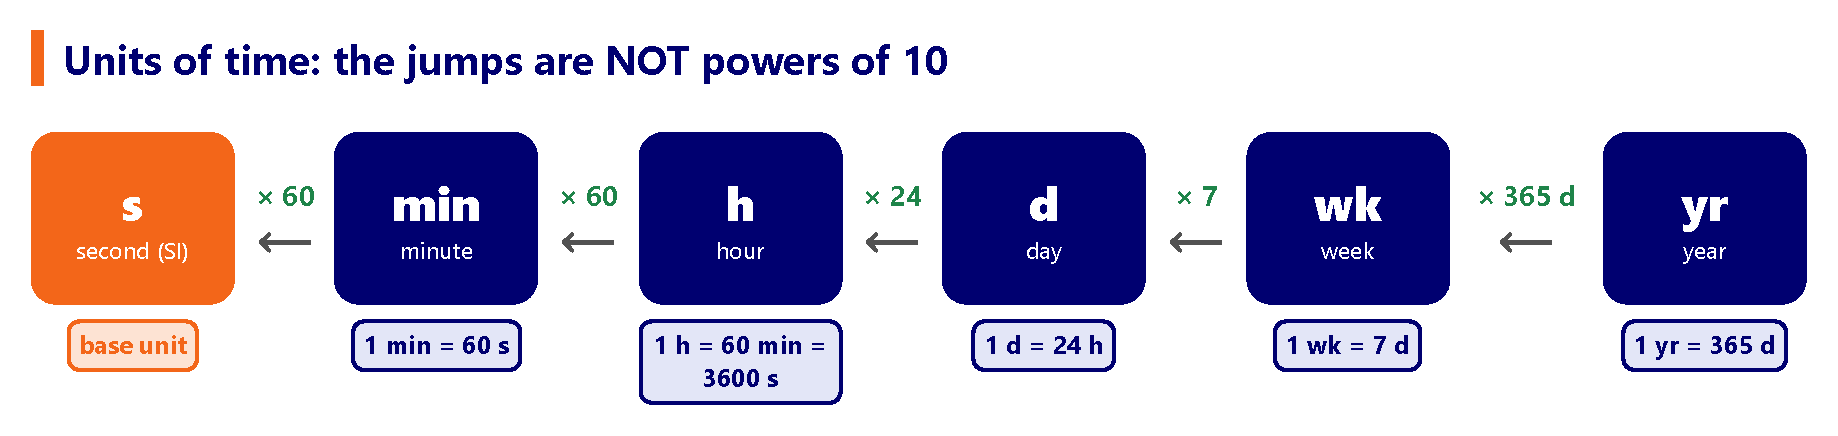
\includegraphics[width=\textwidth]{FigurasSVG/Unit_1_Matter_Measurement/pdf/time_chain.pdf}
    \caption{The chain of time units.}
    \label{fig:u1_time_chain}
\end{figure}

\begin{table}[H]
    \centering
    \renewcommand{\arraystretch}{2.4}
    \begin{tabular}{ll}
        \toprule
        \textbf{Equivalence} & \textbf{Conversion factors} \\
        \midrule
        \(\qty{1}{\minute} = \qty{60}{\s}\) & \(\dfrac{\qty{60}{\s}}{\qty{1}{\minute}}\) or \(\dfrac{\qty{1}{\minute}}{\qty{60}{\s}}\) \\
        \(\qty{1}{\hour} = \qty{60}{\minute} = \qty{3600}{\s}\) & \(\dfrac{\qty{3600}{\s}}{\qty{1}{\hour}}\) or \(\dfrac{\qty{1}{\hour}}{\qty{3600}{\s}}\) \\
        \(\qty{1}{\day} = \qty{24}{\hour}\) & \(\dfrac{\qty{24}{\hour}}{\qty{1}{\day}}\) or \(\dfrac{\qty{1}{\day}}{\qty{24}{\hour}}\) \\
        \(\qty{1}{week} = \qty{7}{\day}\) & \(\dfrac{\qty{7}{\day}}{\qty{1}{week}}\) or \(\dfrac{\qty{1}{week}}{\qty{7}{\day}}\) \\
        \(\qty{1}{year} = \qty{365}{\day}\) & \(\dfrac{\qty{365}{\day}}{\qty{1}{year}}\) or \(\dfrac{\qty{1}{year}}{\qty{365}{\day}}\) \\
        \bottomrule
    \end{tabular}
    \caption{Time equivalences and their conversion factors.}
    \label{tab:u1_time}
\end{table}

\begin{example}
    \textbf{Write \qty{5000}{\s} in hours.}
    \begin{equation*}
        \num{5000}\,\cancelunit{\s} \cdot \dfrac{\qty{1}{\hour}}{\num{3600}\,\cancelunit{\s}} = \dfrac{5000}{3600}\,\unit{\hour} = \textcolor{red}{\qty{1.39}{\hour}}
    \end{equation*}
\end{example}

\begin{example}
    \textbf{How many seconds are there in 2 weeks?} There is no direct equivalence, so we link several factors:
    \begin{equation*}
        \num{2}\,\cancelunit{week} \cdot \dfrac{\num{7}\,\cancelunit{\day}}{1\,\cancelunit{week}} \cdot \dfrac{\num{24}\,\cancelunit{\hour}}{1\,\cancelunit{\day}} \cdot \dfrac{\qty{3600}{\s}}{1\,\cancelunit{\hour}} = \qty{1209600}{\s} \approx \textcolor{red}{\qty{1.21e6}{\s}}
    \end{equation*}
\end{example}

\begin{exercise}
    A film is \qty{135}{\minute} long. How many hours does it last? A song lasts \qty{4.5}{\minute}. How many seconds does it last?
    \begin{solu}
        \(\num{135}\,\unit{\minute} \cdot \dfrac{\qty{1}{\hour}}{\qty{60}{\minute}} = \qty{2.25}{\hour}\). \\
        \(\num{4.5}\,\unit{\minute} \cdot \dfrac{\qty{60}{\s}}{\qty{1}{\minute}} = \qty{270}{\s}\).
    \end{solu}
\end{exercise}

\begin{exercise}
    Convert: \textbf{a)} \qty{3}{\day} \(\to\) \unit{\minute}; \textbf{b)} \qty{90}{\minute} \(\to\) \unit{\hour}; \textbf{c)} \qty{86400}{\s} \(\to\) \unit{\day}; \textbf{d)} \qty{1}{year} \(\to\) weeks.
    \begin{solu}
        a) \(\num{3}\,\unit{\day} \cdot \dfrac{\qty{24}{\hour}}{\qty{1}{\day}} \cdot \dfrac{\qty{60}{\minute}}{\qty{1}{\hour}} = \qty{4320}{\minute}\) \\
        b) \(\num{90}\,\unit{\minute} \cdot \dfrac{\qty{1}{\hour}}{\qty{60}{\minute}} = \qty{1.5}{\hour}\) \\
        c) \(\num{86400}\,\unit{\s} \cdot \dfrac{\qty{1}{\hour}}{\qty{3600}{\s}} \cdot \dfrac{\qty{1}{\day}}{\qty{24}{\hour}} = \qty{1}{\day}\) \\
        d) \(\num{1}\,\unit{year} \cdot \dfrac{\qty{365}{\day}}{\qty{1}{year}} \cdot \dfrac{\qty{1}{week}}{\qty{7}{\day}} \approx \qty{52.1}{weeks}\)
    \end{solu}
\end{exercise}

\begin{exercise}
    You are 12 years old. How many seconds have you lived, approximately? Give the result as a power of 10.
    \begin{solu}
        \(\num{12}\,\unit{year} \cdot \dfrac{\qty{365}{\day}}{\qty{1}{year}} \cdot \dfrac{\qty{24}{\hour}}{\qty{1}{\day}} \cdot \dfrac{\qty{3600}{\s}}{\qty{1}{\hour}} = \qty{378432000}{\s} \approx \qty{3.78e8}{\s}\).
    \end{solu}
\end{exercise}

\begin{exercise}
    Convert these times using conversion factors:
    \begin{enumerate}[label=\letraminuscula]
        \item \(\qty{340}{\minute} \to \unit{\s}\)
        \item \(\qty{6.2}{\hour} \to \unit{\minute}\)
        \item \(\qty{10}{\hour} \to \unit{\s}\)
        \item \(\qty{28}{weeks} \to \unit{\minute}\)
        \item \(\qty{22}{weeks} \to \unit{\hour}\)
    \end{enumerate}
    \begin{solu}
        \begin{enumerate}[label=\alph*)]
            \item \(\num{340}\,\unit{\minute} \cdot \dfrac{\qty{60}{\s}}{\qty{1}{\minute}} = \qty{20400}{\s} \approx \qty{2.04e4}{\s}\)
            \item \(\num{6.2}\,\unit{\hour} \cdot \dfrac{\qty{60}{\minute}}{\qty{1}{\hour}} = \qty{372}{\minute}\)
            \item \(\num{10}\,\unit{\hour} \cdot \dfrac{\qty{3600}{\s}}{\qty{1}{\hour}} = \qty{36000}{\s} = \qty{3.6e4}{\s}\)
            \item \(\num{28}\,\unit{weeks} \cdot \dfrac{\qty{7}{\day}}{\qty{1}{week}} \cdot \dfrac{\qty{24}{\hour}}{\qty{1}{\day}} \cdot \dfrac{\qty{60}{\minute}}{\qty{1}{\hour}} = \qty{282240}{\minute} \approx \qty{2.82e5}{\minute}\)
            \item \(\num{22}\,\unit{weeks} \cdot \dfrac{\qty{7}{\day}}{\qty{1}{week}} \cdot \dfrac{\qty{24}{\hour}}{\qty{1}{\day}} = \qty{3696}{\hour}\)
        \end{enumerate}
    \end{solu}
\end{exercise}

%------------------------------------------------

\subsubsection{Speed}

Speed is a derived quantity (length \(\div\) time), so its unit has \textbf{two} parts. To change it, we use \textbf{two} conversion factors: one for the length (numerator) and one for the time (denominator).

\begin{impt}
    \negsubro{Units with more than one quantity: one unit at a time, in order}

    When a unit is made of two quantities (\unit{\km\per\hour}, \unit{\g\per\mL}\ldots), we do \textbf{not} try to change both at once. We go \textbf{in order}:
    \begin{enumerate}[label=\numberballmDarkTeal]
        \item First we change \textbf{one} of the units (for example, the length: \unit{\km} \(\to\) \unit{\m}) with its own conversion factor.
        \item Then we change the \textbf{other} unit (the time: \unit{\hour} \(\to\) \unit{\s}) with a second conversion factor.
        \item Finally we cancel the units and calculate.
        \item Steps 1 and 2 \textbf{can and should} be done \textbf{all in one line}: we write the first conversion factor and, right after it, the second one, without stopping to calculate the intermediate result. We cancel all the units at the end and do only one calculation.
    \end{enumerate}
    Step by step for \qty{90}{\km\per\hour}:
    \begin{equation*}
        \underbrace{\num{90}\,\dfrac{\cancelunit{\km}}{\unit{\hour}} \cdot \dfrac{\qty{e3}{\m}}{1\,\cancelunit{\km}} = \qty{90000}{\m\per\hour}}_{\text{1st: the length}}
        \quad\Longrightarrow\quad
        \underbrace{\num{90000}\,\dfrac{\unit{\m}}{\cancelunit{\hour}} \cdot \dfrac{1\,\cancelunit{\hour}}{\qty{3600}{\s}} = \qty{25}{\m\per\s}}_{\text{2nd: the time}}
    \end{equation*}
    All in one line (this is how we must do it):
    \begin{equation*}
        \num{90}\,\dfrac{\cancelunit{\km}}{\cancelunit{\hour}} \cdot \underbrace{\dfrac{\qty{e3}{\m}}{1\,\cancelunit{\km}}}_{\text{1st: length}} \cdot \underbrace{\dfrac{1\,\cancelunit{\hour}}{\qty{3600}{\s}}}_{\text{2nd: time}} = \dfrac{\num{90e3}}{3600}\,\unit{\m\per\s} = \qty{25}{\m\per\s}
    \end{equation*}
\end{impt}

\begin{figure}[H]
    \centering
    % [FIGURA ORIGINAL] \includegraphics[width=0.85\textwidth]{Unit_1/speed_shortcut}
    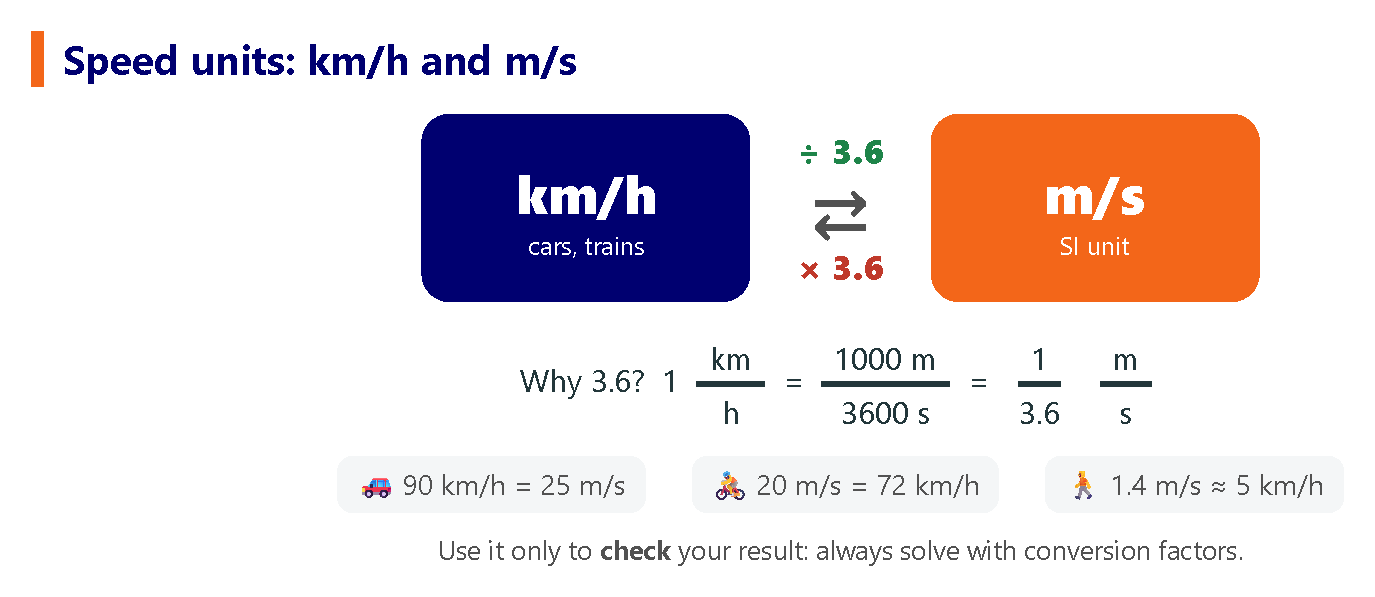
\includegraphics[width=0.85\textwidth]{FigurasSVG/Unit_1_Matter_Measurement/pdf/speed_shortcut.pdf}
    \caption{The two most common units of speed and a quick way to check your result.}
    \label{fig:u1_speed_shortcut}
\end{figure}

\begin{example}
    \textbf{A car travels at \qty{90}{\km\per\hour}. Write this speed in \unit{\m\per\s}.}
    \begin{equation*}
        \num{90}\,\dfrac{\cancelunit{\km}}{\cancelunit{\hour}} \cdot \dfrac{\qty{e3}{\m}}{1\,\cancelunit{\km}} \cdot \dfrac{1\,\cancelunit{\hour}}{\qty{3600}{\s}} = \dfrac{\num{90e3}}{3600}\,\unit{\m\per\s} = \textcolor{red}{\qty{25}{\m\per\s}}
    \end{equation*}
\end{example}

\begin{example}
    \textbf{A cyclist rides at \qty{20}{\m\per\s}. Write this speed in \unit{\km\per\hour}.}
    \begin{equation*}
        \num{20}\,\dfrac{\cancelunit{\m}}{\cancelunit{\s}} \cdot \dfrac{\qty{1}{\km}}{\num{e3}\,\cancelunit{\m}} \cdot \dfrac{\num{3600}\,\cancelunit{\s}}{\qty{1}{\hour}} = \textcolor{red}{\qty{72}{\km\per\hour}}
    \end{equation*}
\end{example}

\begin{marker}
    \textbf{Dividing or multiplying by 3.6 is only a help.} The ``trick'' in the figure (\(\div\,3.6\) to go from \unit{\km\per\hour} to \unit{\m\per\s}, and \(\times\,3.6\) to go back) is only useful to \textbf{check} your result, and it \textbf{only works for that change}: \unit{\km\per\hour} \(\leftrightarrow\) \unit{\m\per\s}. For any other unit of speed (\unit{\cm\per\s}, \unit{\m\per\minute}, \unit{\km\per\minute}\ldots) it gives a wrong answer. The right way, which \textbf{always} works, is to use \textbf{conversion factors}.
\end{marker}

\begin{example}
    \textbf{A tortoise walks at \qty{12}{\m\per\minute}. Write this speed in \unit{\m\per\s}.} Only the time changes, so we need just one factor:
    \begin{equation*}
        \num{12}\,\dfrac{\unit{\m}}{\cancelunit{\minute}} \cdot \dfrac{1\,\cancelunit{\minute}}{\qty{60}{\s}} = \textcolor{red}{\qty{0.2}{\m\per\s}}
    \end{equation*}
\end{example}

\begin{example}
    \textbf{A toy car moves at \qty{45}{\cm\per\s}. Write this speed in \unit{\km\per\hour}.} First the length, then the time:
    \begin{equation*}
        \num{45}\,\dfrac{\cancelunit{\cm}}{\cancelunit{\s}} \cdot \dfrac{\qty{1}{\km}}{\num{e5}\,\cancelunit{\cm}} \cdot \dfrac{\num{3600}\,\cancelunit{\s}}{\qty{1}{\hour}} = \dfrac{\num{45} \cdot \num{3600}}{\num{e5}}\,\unit{\km\per\hour} = \textcolor{red}{\qty{1.62}{\km\per\hour}}
    \end{equation*}
\end{example}

\begin{example}
    \textbf{A plane flies at \qty{15}{\km\per\minute}. Write this speed in \unit{\m\per\s}.} First the length, then the time:
    \begin{equation*}
        \num{15}\,\dfrac{\cancelunit{\km}}{\cancelunit{\minute}} \cdot \dfrac{\qty{e3}{\m}}{1\,\cancelunit{\km}} \cdot \dfrac{1\,\cancelunit{\minute}}{\qty{60}{\s}} = \dfrac{\num{15e3}}{60}\,\unit{\m\per\s} = \textcolor{red}{\qty{250}{\m\per\s}}
    \end{equation*}
\end{example}

\begin{example}
    \textbf{A snail moves at \qty{0.5}{\mm\per\s}. Write this speed in \unit{\m\per\hour}.} First the length, then the time:
    \begin{equation*}
        \num{0.5}\,\dfrac{\cancelunit{\mm}}{\cancelunit{\s}} \cdot \dfrac{\qty{1}{\m}}{\num{e3}\,\cancelunit{\mm}} \cdot \dfrac{\num{3600}\,\cancelunit{\s}}{\qty{1}{\hour}} = \textcolor{red}{\qty{1.8}{\m\per\hour}}
    \end{equation*}
\end{example}

\begin{exercise}
    An athlete runs \qty{100}{\metre} in \qty{11.5}{\s}. Calculate her average speed in \unit{\m\per\s} and in \unit{\km\per\hour}.
    \begin{solu}
        \(v = \dfrac{\qty{100}{\m}}{\qty{11.5}{\s}} \approx \qty{8.70}{\m\per\s}\). \\
        \(\num{8.70}\,\dfrac{\unit{\m}}{\unit{\s}} \cdot \dfrac{\qty{1}{\km}}{\qty{e3}{\m}} \cdot \dfrac{\qty{3600}{\s}}{\qty{1}{\hour}} \approx \qty{31.3}{\km\per\hour}\).
    \end{solu}
\end{exercise}

\begin{exercise}
    Convert these speeds:
    \begin{enumerate}[label=\letraminuscula]
        \item The speed limit on a motorway, \qty{120}{\km\per\hour}, to \unit{\m\per\s}.
        \item The speed of light, \qty{3e5}{\km\per\s}, to \unit{\m\per\s}.
        \item A snail moving at \qty{1.3}{\cm\per\s}, to \unit{\km\per\hour}.
    \end{enumerate}
    \begin{solu}
        \begin{enumerate}[label=\alph*)]
            \item \(\num{120}\,\dfrac{\unit{\km}}{\unit{\hour}} \cdot \dfrac{\qty{e3}{\m}}{\qty{1}{\km}} \cdot \dfrac{\qty{1}{\hour}}{\qty{3600}{\s}} \approx \qty{33.3}{\m\per\s}\)
            \item \(\num{3e5}\,\dfrac{\unit{\km}}{\unit{\s}} \cdot \dfrac{\qty{e3}{\m}}{\qty{1}{\km}} = \qty{3e8}{\m\per\s}\)
            \item \(\num{1.3}\,\dfrac{\unit{\cm}}{\unit{\s}} \cdot \dfrac{\qty{1}{\km}}{\qty{e5}{\cm}} \cdot \dfrac{\qty{3600}{\s}}{\qty{1}{\hour}} \approx \qty{0.047}{\km\per\hour}\)
        \end{enumerate}
    \end{solu}
\end{exercise}

\begin{exercise}
    Convert: \textbf{a)} \qty{36}{\m\per\s} \(\to\) \unit{\km\per\hour}; \textbf{b)} \qty{100}{\km\per\hour} \(\to\) \unit{\m\per\s}.
    \begin{solu}
        a) \(\num{36}\,\dfrac{\unit{\m}}{\unit{\s}} \cdot \dfrac{\qty{1}{\km}}{\qty{e3}{\m}} \cdot \dfrac{\qty{3600}{\s}}{\qty{1}{\hour}} = \qty{129.6}{\km\per\hour}\) \\
        b) \(\num{100}\,\dfrac{\unit{\km}}{\unit{\hour}} \cdot \dfrac{\qty{e3}{\m}}{\qty{1}{\km}} \cdot \dfrac{\qty{1}{\hour}}{\qty{3600}{\s}} \approx \qty{27.8}{\m\per\s}\)
    \end{solu}
\end{exercise}

%------------------------------------------------

\subsubsection{Density}

Density also combines two quantities (mass and volume), so we usually need \textbf{two} conversion factors, one for each unit. Remember to go \textbf{in order}: first we change the unit of mass and then the unit of volume, always \textbf{one at a time}.

\begin{example}
    \textbf{Write the density of ketchup, \qty{1.16}{\g\per\mL}, in \unit{\kg\per\cubic\metre}.}
    \begin{enumerate}[label=\numberballmDarkTeal]
        \item Equivalences: \(\qty{1}{\kg} = \qty{e3}{\g}\) and \(\qty{1}{\cubic\metre} = \qty{1}{\kilo\litre} = \qty{e6}{\mL}\).
        \item Conversion factors:
        \(
            \num{1.16}\,\dfrac{\cancelunit{\g}}{\cancelunit{\mL}} \cdot \dfrac{\qty{1}{\kg}}{\num{e3}\,\cancelunit{\g}} \cdot \dfrac{\num{e6}\,\cancelunit{\mL}}{\qty{1}{\cubic\m}}
        \)
        \item Result: \(\textcolor{red}{\qty{1.16e3}{\kg\per\cubic\metre}} = \qty{1160}{\kg\per\cubic\m}\).
    \end{enumerate}
\end{example}

\begin{exercise}
    Mercury is a liquid metal. \qty{1}{\litre} of mercury has a mass of \qty{13.59}{\kg}. Write its density in \unit{\kg\per\cubic\metre}.
    \begin{solu}
        \(d = \dfrac{\qty{13.59}{\kg}}{\qty{1}{\litre}} \cdot \dfrac{\qty{e3}{\litre}}{\qty{1}{\cubic\m}} = \qty{1.359e4}{\kg\per\cubic\metre}\).
    \end{solu}
\end{exercise}

\begin{exercise}
    The air we breathe has a density of approximately \qty{1.29}{\kg\per\cubic\metre}. Write it in \unit{\g\per\litre}.
    \begin{solu}
        \(d = \num{1.29}\,\dfrac{\unit{\kg}}{\unit{\cubic\m}} \cdot \dfrac{\qty{e3}{\g}}{\qty{1}{\kg}} \cdot \dfrac{\qty{1}{\cubic\m}}{\qty{e3}{\litre}} = \qty{1.29}{\g\per\litre}\).
    \end{solu}
\end{exercise}

\begin{exercise}
    A certain type of wood has a density of \qty{750}{\kg\per\cubic\metre}. Write it in \unit{\g\per\mL}, and decide whether this wood floats in water.
    \begin{solu}
        \(\num{750}\,\dfrac{\unit{\kg}}{\unit{\cubic\m}} \cdot \dfrac{\qty{e3}{\g}}{\qty{1}{\kg}} \cdot \dfrac{\qty{1}{\cubic\m}}{\qty{e6}{\mL}} = \qty{0.75}{\g\per\mL}\). \\
        Since \(\qty{0.75}{\g\per\mL} < \qty{1.00}{\g\per\mL}\), this wood \textbf{floats} in water.
    \end{solu}
\end{exercise}

\begin{exercise}
    Convert these densities using conversion factors:
    \begin{enumerate}[label=\letraminuscula]
        \item \(\qty{1.05}{\kg\per\cubic\cm} \to \unit{\hecto\gram\per\cubic\mm}\)
        \item \(\qty{0.25}{\g\per\mL} \to \unit{\kg\per\cubic\m}\)
        \item \(\qty{0.05}{\kg\per\cubic\cm} \to \unit{\g\per\mL}\)
    \end{enumerate}
    \begin{solu}
        \begin{enumerate}[label=\alph*)]
            \item \(\num{1.05}\,\dfrac{\unit{\kg}}{\unit{\cubic\cm}} \cdot \dfrac{\qty{e1}{\hecto\gram}}{\qty{1}{\kg}} \cdot \left(\dfrac{\qty{1}{\cm}}{\qty{e1}{\mm}}\right)^{3} = \num{1.05}\,\dfrac{\unit{\kg}}{\unit{\cubic\cm}} \cdot \dfrac{\qty{e1}{\hecto\gram}}{\qty{1}{\kg}} \cdot \dfrac{\qty{1}{\cubic\cm}}{\qty{e3}{\cubic\mm}} = \qty{1.05e-2}{\hecto\gram\per\cubic\mm}\)
            \item \(\num{0.25}\,\dfrac{\unit{\g}}{\unit{\mL}} \cdot \dfrac{\qty{1}{\kg}}{\qty{e3}{\g}} \cdot \dfrac{\qty{e6}{\mL}}{\qty{1}{\cubic\m}} = \qty{250}{\kg\per\cubic\m} = \qty{2.5e2}{\kg\per\cubic\m}\)
            \item \(\num{0.05}\,\dfrac{\unit{\kg}}{\unit{\cubic\cm}} \cdot \dfrac{\qty{e3}{\g}}{\qty{1}{\kg}} \cdot \dfrac{\qty{1}{\cubic\cm}}{\qty{1}{\mL}} = \qty{50}{\g\per\mL}\)
        \end{enumerate}
    \end{solu}
\end{exercise}

\begin{exercise}
    Isolate the volume, calculate it and then change it to \unit{\cubic\m}:
    \begin{enumerate}[label=\letraminuscula]
        \item A gold bar has a density of \qty{19}{\g\per\cubic\cm} and a mass of \qty{9500}{\g}. Calculate the volume of the gold bar, in \unit{\cubic\m}.
        \item A cricket ball has a density of \qty{0.8}{\g\per\cubic\cm} and a mass of \qty{165}{\g}. Calculate the volume of the cricket ball, in \unit{\cubic\m}.
    \end{enumerate}
    \begin{solu}
        \begin{enumerate}[label=\alph*)]
            \item \(V = \dfrac{m}{d} = \dfrac{\qty{9500}{\g}}{\qty{19}{\g\per\cubic\cm}} = \qty{500}{\cubic\cm}\). \\
            In \unit{\cubic\m}: \(\num{500}\,\unit{\cubic\cm} \cdot \left(\dfrac{\qty{1}{\m}}{\qty{e2}{\cm}}\right)^{3} = \num{500}\,\unit{\cubic\cm} \cdot \dfrac{\qty{1}{\cubic\m}}{\qty{e6}{\cubic\cm}} = \qty{5e-4}{\cubic\m}\)
            \item \(V = \dfrac{m}{d} = \dfrac{\qty{165}{\g}}{\qty{0.8}{\g\per\cubic\cm}} = \qty{206.25}{\cubic\cm}\). \\
            In \unit{\cubic\m}: \(\num{206.25}\,\unit{\cubic\cm} \cdot \left(\dfrac{\qty{1}{\m}}{\qty{e2}{\cm}}\right)^{3} = \num{206.25}\,\unit{\cubic\cm} \cdot \dfrac{\qty{1}{\cubic\m}}{\qty{e6}{\cubic\cm}} \approx \qty{2.06e-4}{\cubic\m}\)
        \end{enumerate}
    \end{solu}
\end{exercise}

%------------------------------------------------

\subsubsection{Different units of the same quantity: pressure and energy}

Some quantities are measured with units that \textbf{do not} come from the same prefix staircase, for historical reasons or because they are more practical in everyday life. We change between them with conversion factors built from their equivalences.

\begin{figure}[H]
    \centering
    % [FIGURA ORIGINAL] \includegraphics[width=\textwidth]{Unit_1/pressure_energy}
    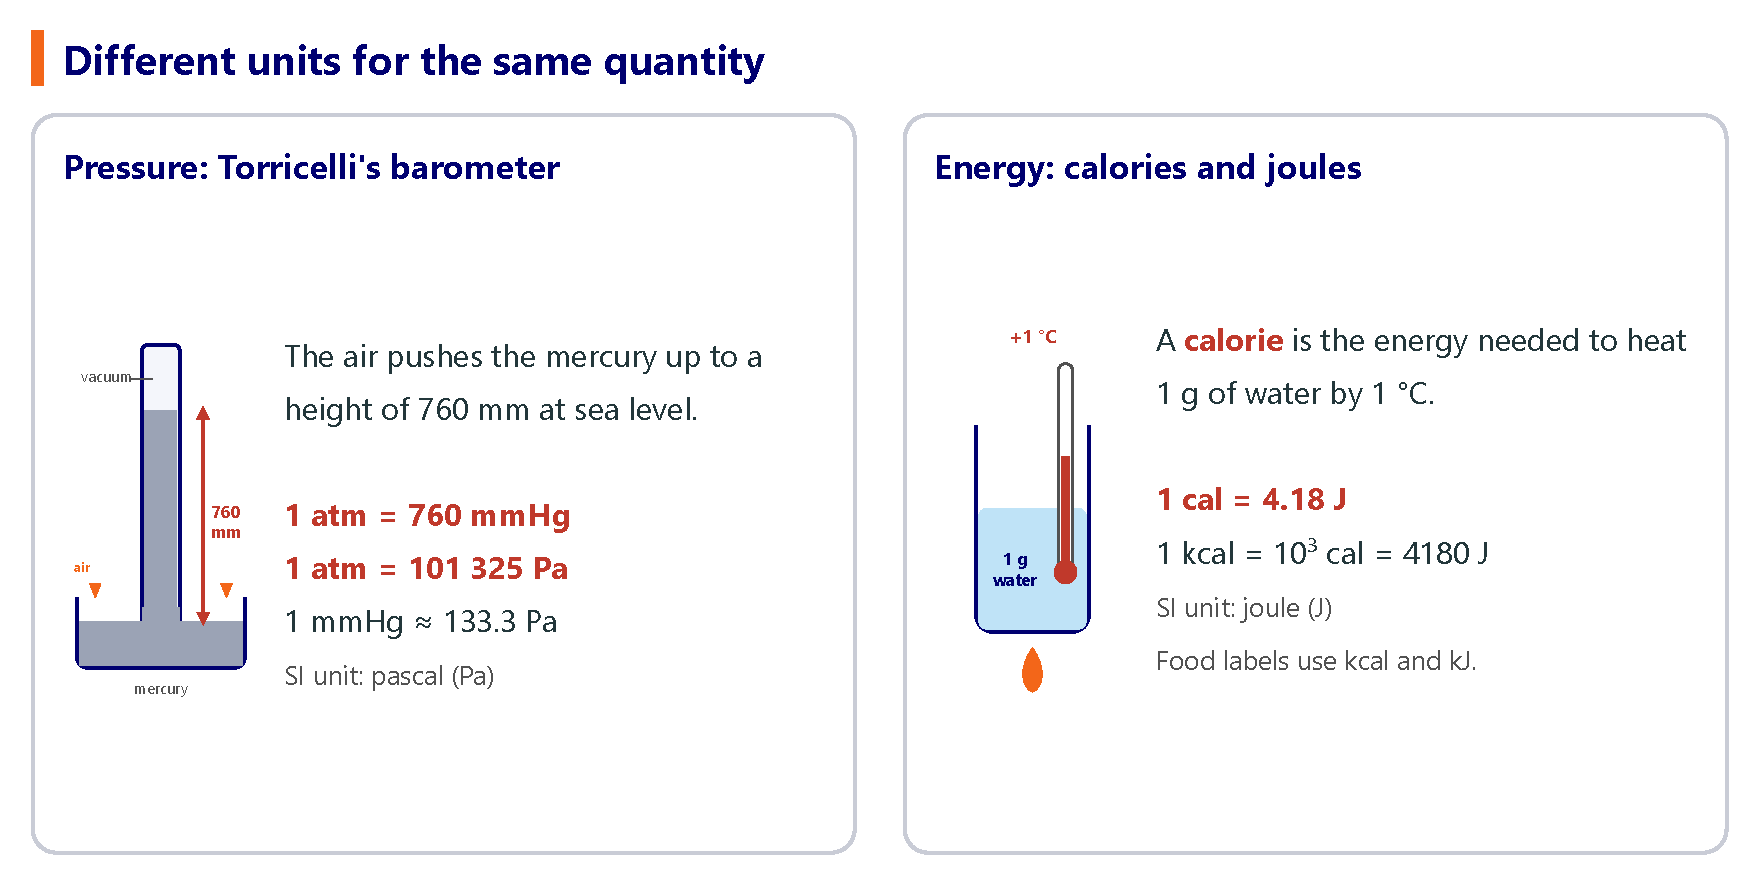
\includegraphics[width=\textwidth]{FigurasSVG/Unit_1_Matter_Measurement/pdf/pressure_energy.pdf}
    \caption{Where the atmosphere, the millimetre of mercury and the calorie come from.}
    \label{fig:u1_pressure_energy}
\end{figure}

\begin{table}[H]
    \centering
    \renewcommand{\arraystretch}{1.4}
    \begin{tabular}{lcp{6.5cm}}
        \toprule
        \textbf{Quantity} & \textbf{SI unit} & \textbf{Equivalences} \\
        \midrule
        Pressure & pascal (\unit{\Pa}) & \(\qty{1}{\atmospher} = \qty{760}{\mmhg}\) \newline \(\qty{1}{\atmospher} = \qty{101325}{\Pa} \approx \qty{1.013e5}{\Pa}\) \\
        Energy & joule (\unit{\J}) & \(\qty{1}{\calorie} = \qty{4.18}{\J}\) \newline \(\qty{1}{\kilo\calorie} = \qty{e3}{\calorie}\) \\
        \bottomrule
    \end{tabular}
    \caption{Units of pressure and energy and their equivalences.}
    \label{tab:u1_pressure_energy}
\end{table}

\begin{example}
    \textbf{Pressure.} The air pressure in a tyre is \qty{1.5}{\atmospher}. Write it in \unit{\Pa} and in \unit{\mmhg}.
    \begin{equation*}
        \num{1.5}\,\cancelunit{\atmospher} \cdot \dfrac{\qty{101325}{\Pa}}{1\,\cancelunit{\atmospher}} \approx \textcolor{red}{\qty{1.52e5}{\Pa}}
        \qquad\qquad
        \num{1.5}\,\cancelunit{\atmospher} \cdot \dfrac{\qty{760}{\mmhg}}{1\,\cancelunit{\atmospher}} = \textcolor{red}{\qty{1140}{\mmhg}}
    \end{equation*}
\end{example}

\begin{example}
    \textbf{Pressure.} Write \qty{380}{\mmhg} in pascals. There is no direct equivalence, so we go through atmospheres:
    \begin{equation*}
        \num{380}\,\cancelunit{\mmhg} \cdot \dfrac{1\,\cancelunit{\atmospher}}{\num{760}\,\cancelunit{\mmhg}} \cdot \dfrac{\qty{101325}{\Pa}}{1\,\cancelunit{\atmospher}} \approx \textcolor{red}{\qty{5.07e4}{\Pa}}
    \end{equation*}
\end{example}

\begin{example}
    \textbf{Energy.} A chocolate bar gives \qty{250}{\kilo\calorie}. Write this energy in joules.
    \begin{equation*}
        \num{250}\,\cancelunit{\kilo\calorie} \cdot \dfrac{\num{e3}\,\cancelunit{\calorie}}{1\,\cancelunit{\kilo\calorie}} \cdot \dfrac{\qty{4.18}{\J}}{1\,\cancelunit{\calorie}} = \textcolor{red}{\qty{1.045e6}{\J}}
    \end{equation*}
\end{example}

\begin{exercise}
    Convert these pressures:
    \begin{enumerate}[label=\letraminuscula]
        \item \qty{0.33}{\atmospher} (air pressure at the top of Mount Everest) to \unit{\mmhg}.
        \item \qty{120}{\mmhg} (a normal blood pressure) to \unit{\atmospher} and to \unit{\Pa}.
        \item \qty{2e5}{\Pa} to \unit{\atmospher}.
    \end{enumerate}
    \begin{solu}
        \begin{enumerate}[label=\alph*)]
            \item \(\num{0.33}\,\unit{\atmospher} \cdot \dfrac{\qty{760}{\mmhg}}{\qty{1}{\atmospher}} \approx \qty{251}{\mmhg}\)
            \item \(\num{120}\,\unit{\mmhg} \cdot \dfrac{\qty{1}{\atmospher}}{\qty{760}{\mmhg}} \approx \qty{0.158}{\atmospher}\); \quad
            \(\num{120}\,\unit{\mmhg} \cdot \dfrac{\qty{1}{\atmospher}}{\qty{760}{\mmhg}} \cdot \dfrac{\qty{101325}{\Pa}}{\qty{1}{\atmospher}} \approx \qty{1.60e4}{\Pa}\)
            \item \(\num{2e5}\,\unit{\Pa} \cdot \dfrac{\qty{1}{\atmospher}}{\qty{101325}{\Pa}} \approx \qty{1.97}{\atmospher}\)
        \end{enumerate}
    \end{solu}
\end{exercise}

\begin{exercise}
    Convert these energies:
    \begin{enumerate}[label=\letraminuscula]
        \item \qty{836}{\J} to calories.
        \item A yoghurt label says \qty{400}{\kilo\joule}. Write this energy in \unit{\kilo\calorie}.
        \item \qty{1.5}{\kilo\calorie} to \unit{\J}.
    \end{enumerate}
    \begin{solu}
        \begin{enumerate}[label=\alph*)]
            \item \(\num{836}\,\unit{\J} \cdot \dfrac{\qty{1}{\calorie}}{\qty{4.18}{\J}} = \qty{200}{\calorie}\)
            \item \(\num{400}\,\unit{\kilo\joule} \cdot \dfrac{\qty{e3}{\J}}{\qty{1}{\kilo\joule}} \cdot \dfrac{\qty{1}{\calorie}}{\qty{4.18}{\J}} \cdot \dfrac{\qty{1}{\kilo\calorie}}{\qty{e3}{\calorie}} \approx \qty{95.7}{\kilo\calorie}\)
            \item \(\num{1.5}\,\unit{\kilo\calorie} \cdot \dfrac{\qty{e3}{\calorie}}{\qty{1}{\kilo\calorie}} \cdot \dfrac{\qty{4.18}{\J}}{\qty{1}{\calorie}} = \qty{6270}{\J}\)
        \end{enumerate}
    \end{solu}
\end{exercise}

%----------------------------------------------------------------------------------------

\subsection{Scientific notation}

% Calculator keys: \calckey{EXP} draws one key; \keys{3 . 2 EXP 3} draws one key per word
\providecommand{\calckey}[1]{{\setlength{\fboxsep}{1.5pt}\fbox{\footnotesize\sffamily\strut #1}}}
\ExplSyntaxOn
\providecommand{\keys}[1]{\seq_set_split:Nnn \l_tmpa_seq {~} {#1} \seq_map_inline:Nn \l_tmpa_seq {\calckey{##1}\,} \unskip}
\ExplSyntaxOff
% Red decimal comma used to show where the comma ends up in the examples
\providecommand{\redcomma}{\textcolor{red}{\mathbf{,}}}

In science we often find numbers that are very big or very small. The distance from the Earth to the Sun is about \qty{150000000}{\km}, and a bacterium measures about \qty{0.000002}{\m}. Writing and reading so many zeros is slow and it is very easy to make mistakes. That is why scientists use \negsubro{scientific notation}. You have already used it with conversion factors: \(\qty{1}{\km} = \qty{e3}{\m}\).

\begin{definition}[Scientific notation]
    A way of writing a number as the product of a \textbf{coefficient} and a \textbf{power of 10}:
    \begin{equation*}
        a \cdot 10^{n}
    \end{equation*}
    \begin{itemize}
        \item The \textbf{coefficient} \(a\) is a number from 1 to 9,99\ldots: it has \textbf{only one digit, different from zero, before the decimal comma}.
        \item The \textbf{exponent} \(n\) is a whole number: \textbf{positive} for numbers greater than 10, and \textbf{negative} for numbers smaller than 1.
    \end{itemize}
\end{definition}

\begin{figure}[H]
    \centering
    % [FIGURA ORIGINAL] \includegraphics[width=\textwidth]{Unit_1/sci_notation_parts}
    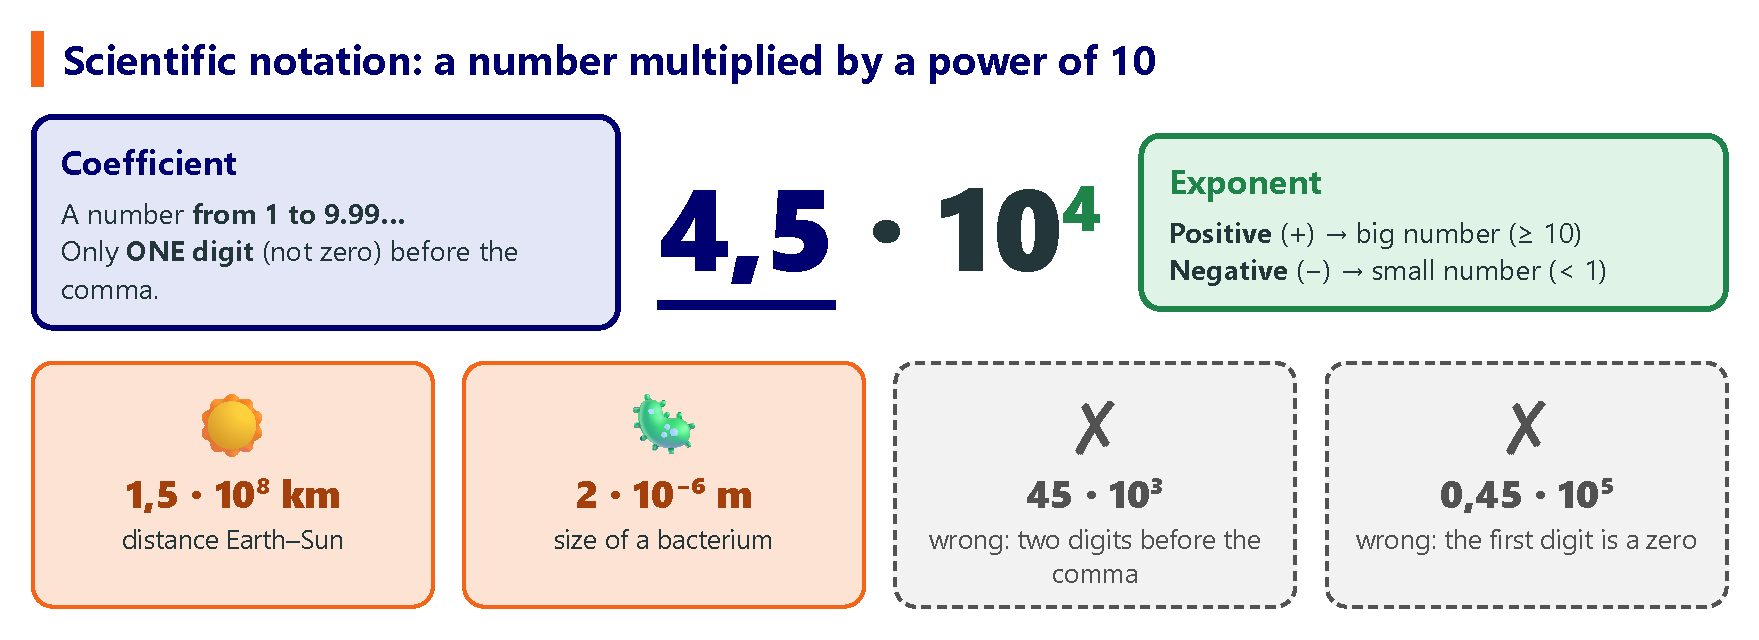
\includegraphics[width=\textwidth]{FigurasSVG/Unit_1_Matter_Measurement/pdf/sci_notation_parts.pdf}
    \caption{The two parts of a number in scientific notation, with correct and incorrect examples.}
    \label{fig:u1_sci_notation_parts}
\end{figure}

\begin{impt}
    \negsubro{Scientific notation does not change the number!} It is the \textbf{same number written in a different way}, just as ``a half'', \(\frac{1}{2}\) and \(0{,}5\) are the same amount:
    \begin{equation*}
        45\,000 = 4{,}5 \cdot 10^{4} = 45 \cdot 10^{3} = 450 \cdot 10^{2} = 0{,}45 \cdot 10^{5}
    \end{equation*}
    All of them are worth exactly the same. Of all these ways of writing it, only \(4{,}5 \cdot 10^{4}\) is \textbf{correct scientific notation}, because it has only one digit (different from zero) before the comma.
\end{impt}

Remember what a power of 10 means: the exponent tells us how many places the comma moves.

\begin{table}[H]
    \centering
    \renewcommand{\arraystretch}{1.35}
    \begin{tabular}{cc@{\hspace{1.5cm}}cc}
        \toprule
        \textbf{Power} & \textbf{Decimal} & \textbf{Power} & \textbf{Decimal} \\
        \midrule
        \(10^{1}\) & \num{10}    & \(10^{-1}\) & \num{0.1}   \\
        \(10^{2}\) & \num{100}   & \(10^{-2}\) & \num{0.01}  \\
        \(10^{3}\) & \num{1000}  & \(10^{-3}\) & \num{0.001} \\
        \(10^{4}\) & \num{10000} & \(10^{-4}\) & \num{0.0001} \\
        \bottomrule
    \end{tabular}
    \caption{Positive powers of 10 are numbers \textbf{greater than 1}; negative powers of 10 are numbers \textbf{smaller than 1}. \(10^{0} = 1\).}
    \label{tab:u1_powers_of_ten}
\end{table}

\begin{figure}[H]
    \centering
    % [FIGURA ORIGINAL] \includegraphics[width=\textwidth]{Unit_1/sci_notation_to}
    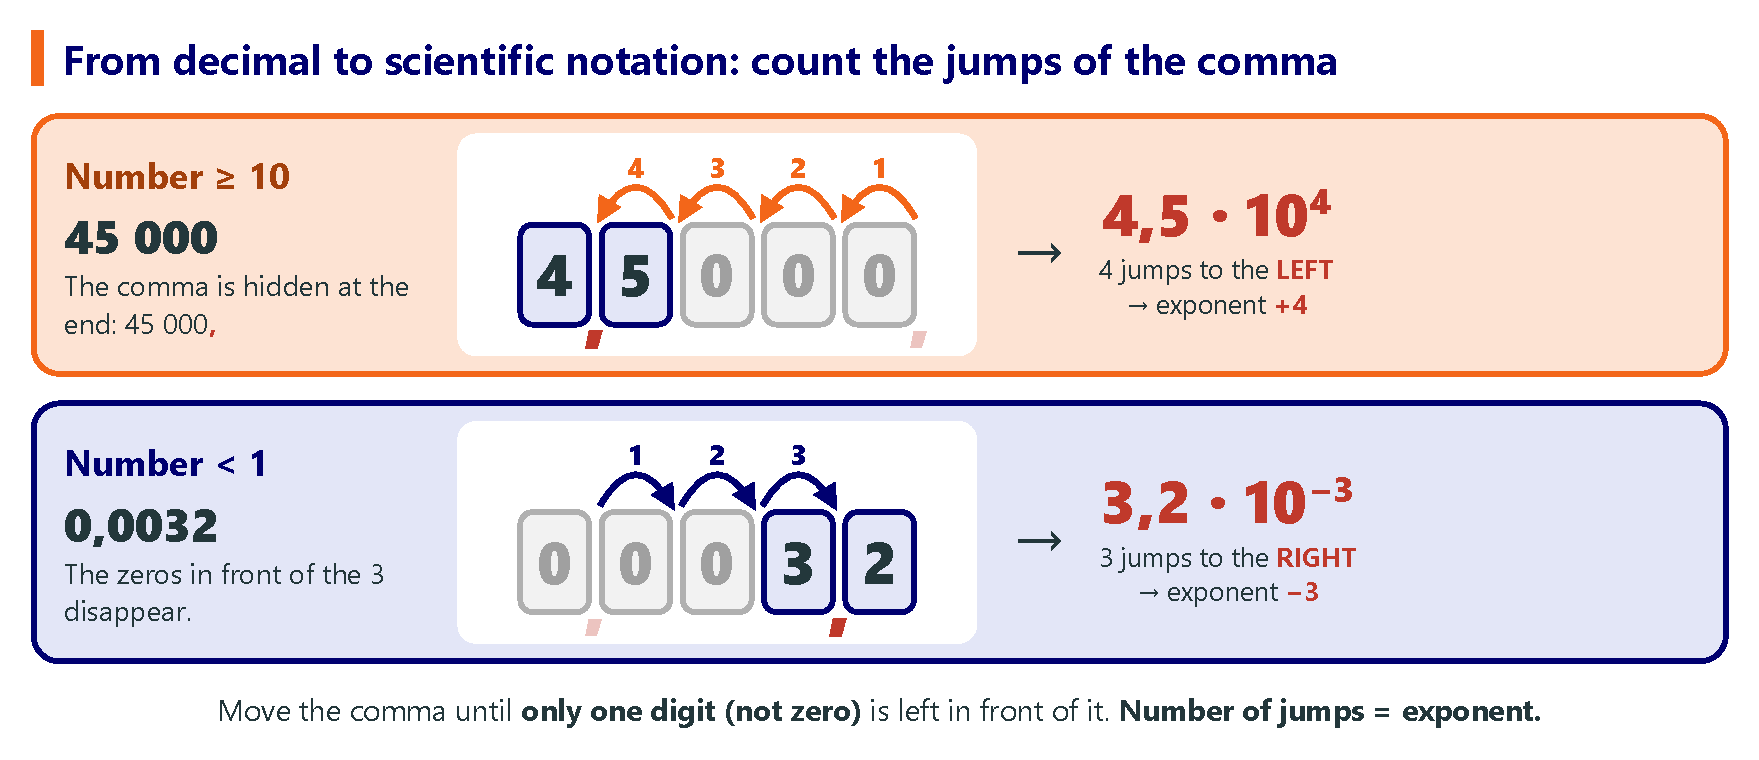
\includegraphics[width=\textwidth]{FigurasSVG/Unit_1_Matter_Measurement/pdf/sci_notation_to.pdf}
    \caption{To write a number in scientific notation we count how many places the comma jumps.}
    \label{fig:u1_sci_notation_to}
\end{figure}

%------------------------------------------------

\subsubsection{Numbers greater than 1 to scientific notation}

\negsubro{Method, step by step}:
\begin{enumerate}[label=\numberballmDarkTeal]
    \item Find the decimal comma. If the number has no comma, it is \textbf{hidden at the end}: \(45\,000 = 45\,000\redcomma\)
    \item Move the comma to the \textbf{left}, one place at a time, until \textbf{only one digit} is left in front of it. \textbf{Count the jumps}.
    \item Write the \textbf{coefficient}: the digits with the comma in its new place. The zeros at the end are not needed: \(4\redcomma 5000 = 4{,}5\).
    \item The \textbf{exponent} is the \textbf{number of jumps}, and it is \textbf{positive}: the number was big.
    \item Check: \(\num{4.5e4}\) must be equal to the starting number.
\end{enumerate}

\begin{example}
    \textbf{Write \num{45000} in scientific notation.}
    \begin{enumerate}[label=\numberballmDarkTeal]
        \item Hidden comma at the end: \(45\,000\redcomma\)
        \item We move the comma 4 places to the left: \(45\,000\redcomma \to 4500\redcomma 0 \to 450\redcomma 00 \to 45\redcomma 000 \to 4\redcomma 5000\) \(\Rightarrow\) \textbf{4 jumps}.
        \item Coefficient: \(4{,}5\).
        \item Exponent: \(+4\).
        \item \(\textcolor{red}{\num{45000} = \num{4.5e4}}\)
    \end{enumerate}
\end{example}

\begin{example}
    \textbf{Write \num{6700} and \num{380.5} in scientific notation.}
    \begin{itemize}
        \item \(6700\redcomma \to 6\redcomma 700\): 3 jumps to the left \(\Rightarrow\) \(\textcolor{red}{\num{6700} = \num{6.7e3}}\)
        \item \(380{,}5 \to 3\redcomma 805\): 2 jumps to the left \(\Rightarrow\) \(\textcolor{red}{\num{380.5} = \num{3.805e2}}\)
    \end{itemize}
\end{example}

%------------------------------------------------

\subsubsection{Numbers smaller than 1 to scientific notation}

\negsubro{Method, step by step}:
\begin{enumerate}[label=\numberballmDarkTeal]
    \item Find the decimal comma: \(0{,}0032\).
    \item Move the comma to the \textbf{right}, one place at a time, until it is just after the \textbf{first digit that is not zero}. \textbf{Count the jumps}.
    \item Write the \textbf{coefficient}: the zeros in front disappear: \(0003\redcomma 2 = 3{,}2\).
    \item The \textbf{exponent} is the \textbf{number of jumps}, and it is \textbf{negative}: the number was smaller than 1.
    \item Check: \(\num{3.2e-3}\) must be equal to the starting number.
\end{enumerate}

\begin{example}
    \textbf{Write \num{0.0032} in scientific notation.}
    \begin{enumerate}[label=\numberballmDarkTeal]
        \item Comma: \(0\redcomma 0032\)
        \item We move the comma 3 places to the right: \(0\redcomma 0032 \to 00\redcomma 032 \to 000\redcomma 32 \to 0003\redcomma 2\) \(\Rightarrow\) \textbf{3 jumps}.
        \item Coefficient: \(3{,}2\).
        \item Exponent: \(-3\).
        \item \(\textcolor{red}{\num{0.0032} = \num{3.2e-3}}\)
    \end{enumerate}
\end{example}

\begin{example}
    \textbf{Write \num{0.07} and \num{0.125} in scientific notation.}
    \begin{itemize}
        \item \(0{,}07 \to 007\redcomma\): 2 jumps to the right \(\Rightarrow\) \(\textcolor{red}{\num{0.07} = \num{7e-2}}\)
        \item \(0{,}125 \to 01\redcomma 25\): 1 jump to the right \(\Rightarrow\) \(\textcolor{red}{\num{0.125} = \num{1.25e-1}}\)
    \end{itemize}
\end{example}

\begin{impt}
    \textbf{Which way does the comma move?}
    \begin{itemize}
        \item Big number (greater than 10) \(\to\) the comma jumps to the \textbf{left} \(\to\) exponent \textbf{positive}.
        \item Small number (smaller than 1) \(\to\) the comma jumps to the \textbf{right} \(\to\) exponent \textbf{negative}.
        \item Number between 1 and 10 \(\to\) the comma does not move \(\to\) exponent \textbf{0}: \(7{,}2 = \num{7.2e0}\).
    \end{itemize}
\end{impt}

%------------------------------------------------

\subsubsection{From scientific notation to decimal}

Now we do the opposite: we start from \(a \cdot 10^{n}\) and we want the normal (decimal) number. The \textbf{exponent} tells us how many places the comma jumps, and its \textbf{sign} tells us in which direction.

\begin{figure}[H]
    \centering
    % [FIGURA ORIGINAL] \includegraphics[width=\textwidth]{Unit_1/sci_notation_back}
    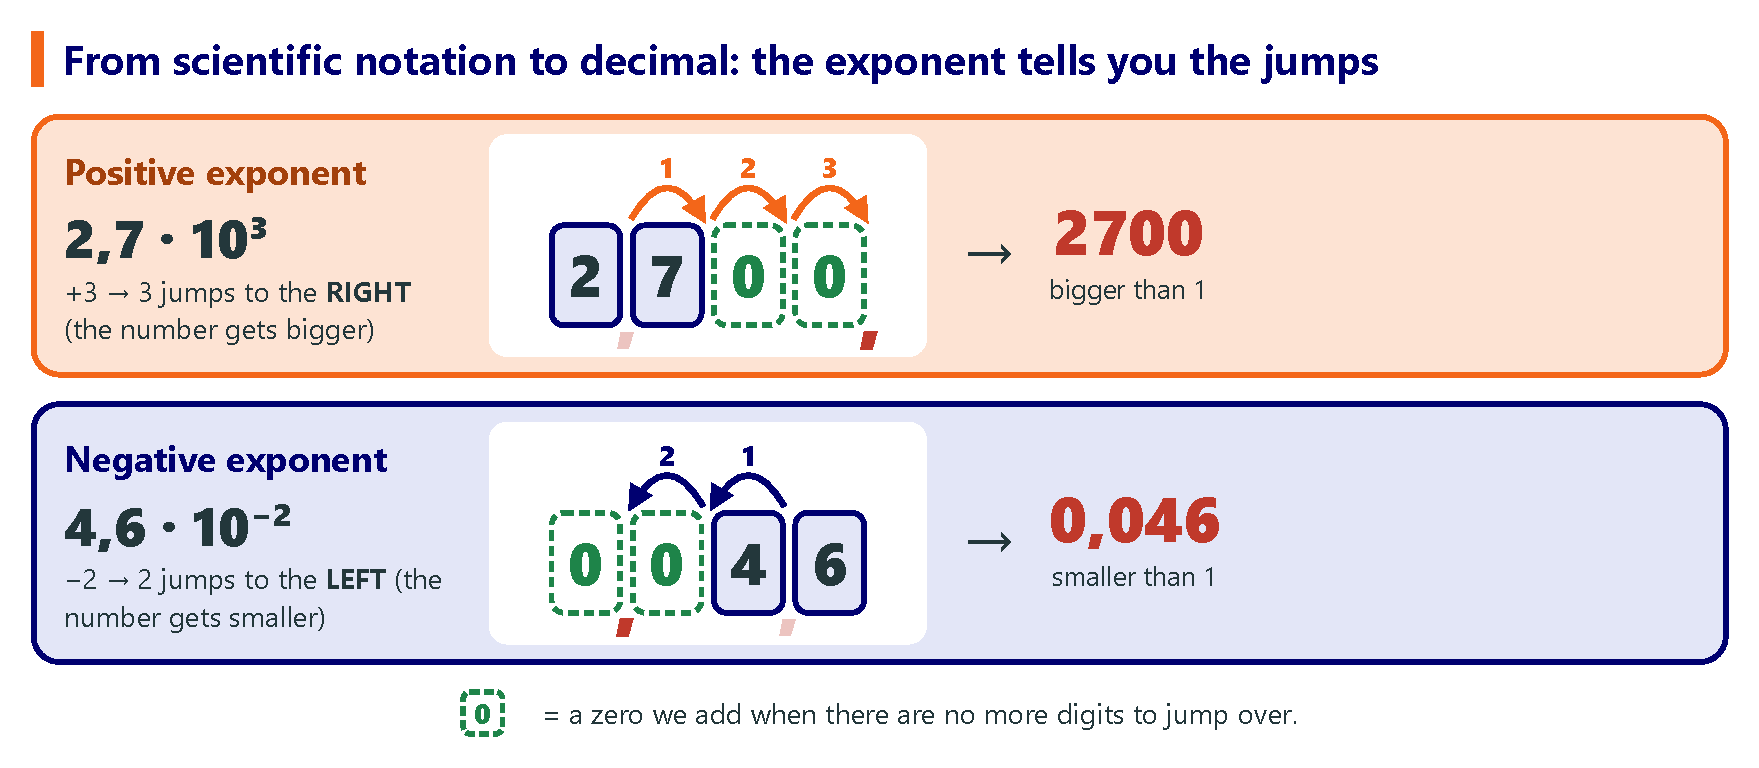
\includegraphics[width=\textwidth]{FigurasSVG/Unit_1_Matter_Measurement/pdf/sci_notation_back.pdf}
    \caption{From scientific notation to decimal: positive exponent, the comma jumps to the right; negative exponent, the comma jumps to the left.}
    \label{fig:u1_sci_notation_back}
\end{figure}

\negsubro{Method, step by step}:
\begin{enumerate}[label=\numberballmDarkTeal]
    \item Look at the \textbf{sign of the exponent}:
    \begin{itemize}
        \item \textbf{Positive} \(\to\) the comma jumps to the \textbf{right} (the number gets \textbf{bigger}).
        \item \textbf{Negative} \(\to\) the comma jumps to the \textbf{left} (the number gets \textbf{smaller}).
    \end{itemize}
    \item Move the comma as many places as the exponent says.
    \item If there are no more digits to jump over, \textbf{add zeros}.
    \item If the comma ends up at the very front, write a \textbf{0} before it: \(\redcomma 046 \to 0{,}046\).
\end{enumerate}

\begin{example}
    \textbf{Positive exponent: write \num{2.7e3} as a decimal number.}
    \begin{enumerate}[label=\numberballmDarkTeal]
        \item Exponent \(+3\): 3 jumps to the \textbf{right}.
        \item \(2\redcomma 7 \to 27\redcomma \to 270\redcomma \to 2700\redcomma\) (we have added two zeros).
        \item \(\textcolor{red}{\num{2.7e3} = \num{2700}}\)
    \end{enumerate}
    More examples: \(\num{5e2} = 500\); \quad \(\num{1.25e3} = 1250\); \quad \(\num{3.06e4} = \num{30600}\).
\end{example}

\begin{example}
    \textbf{Negative exponent: write \num{4.6e-2} as a decimal number.}
    \begin{enumerate}[label=\numberballmDarkTeal]
        \item Exponent \(-2\): 2 jumps to the \textbf{left}.
        \item \(4\redcomma 6 \to \redcomma 46 \to \redcomma 046\) (we have added one zero).
        \item We write a 0 in front of the comma: \(\textcolor{red}{\num{4.6e-2} = \num{0.046}}\)
    \end{enumerate}
    More examples: \(\num{8e-3} = \num{0.008}\); \quad \(\num{1.5e-1} = \num{0.15}\); \quad \(\num{9.2e-4} = \num{0.00092}\).
\end{example}

\begin{marker}
    \textbf{Quick check}: if the exponent is positive, your decimal number must be \textbf{greater than 1}; if it is negative, it must start with \textbf{0,\ldots}. If not, you moved the comma in the wrong direction!
\end{marker}

\begin{exercise}
    Write these numbers in scientific notation:
    \begin{enumerate}[label=\letraminuscula]
        \item \num{3400}
        \item \num{52000}
        \item \num{700000}
        \item \num{186}
        \item \num{0.045}
        \item \num{0.0007}
        \item \num{0.00128}
        \item \num{0.5}
    \end{enumerate}
    \begin{solu}
        \begin{enumerate}[label=\alph*)]
            \item 3 jumps to the left: \(\num{3.4e3}\)
            \item 4 jumps to the left: \(\num{5.2e4}\)
            \item 5 jumps to the left: \(\num{7e5}\)
            \item 2 jumps to the left: \(\num{1.86e2}\)
            \item 2 jumps to the right: \(\num{4.5e-2}\)
            \item 4 jumps to the right: \(\num{7e-4}\)
            \item 3 jumps to the right: \(\num{1.28e-3}\)
            \item 1 jump to the right: \(\num{5e-1}\)
        \end{enumerate}
    \end{solu}
\end{exercise}

\begin{exercise}
    Write these numbers as decimal numbers:
    \begin{enumerate}[label=\letraminuscula]
        \item \num{3.1e2}
        \item \num{6e4}
        \item \num{1.25e3}
        \item \num{9e-1}
        \item \num{2.4e-3}
        \item \num{7.05e-2}
    \end{enumerate}
    \begin{solu}
        \begin{enumerate}[label=\alph*)]
            \item 2 jumps to the right: \num{310}
            \item 4 jumps to the right: \num{60000}
            \item 3 jumps to the right: \num{1250}
            \item 1 jump to the left: \num{0.9}
            \item 3 jumps to the left: \num{0.0024}
            \item 2 jumps to the left: \num{0.0705}
        \end{enumerate}
    \end{solu}
\end{exercise}

\begin{exercise}
    These numbers are \textbf{not} correctly written in scientific notation. Explain the mistake and write them correctly: \num{23e4}, \num{0.8e3}, \num{15e-3}.
    \begin{solu}
        \begin{itemize}
            \item \(\num{23e4}\): two digits before the comma. \(\num{23e4} = \num{230000} = \num{2.3e5}\).
            \item \(\num{0.8e3}\): the digit before the comma is a zero. \(\num{0.8e3} = \num{800} = \num{8e2}\).
            \item \(\num{15e-3}\): two digits before the comma. \(\num{15e-3} = \num{0.015} = \num{1.5e-2}\).
        \end{itemize}
    \end{solu}
\end{exercise}

\begin{exercise}
    Write the numbers in these sentences in scientific notation:
    \begin{enumerate}[label=\letraminuscula]
        \item Sound travels through air at \qty{340}{\m\per\s}.
        \item A human hair is about \qty{0.00008}{\m} thick.
        \item The Moon is about \qty{384000}{\km} away from the Earth.
        \item A grain of sand has a mass of about \qty{0.0006}{\g}.
    \end{enumerate}
    \begin{solu}
        \begin{enumerate}[label=\alph*)]
            \item \(\qty{3.4e2}{\m\per\s}\)
            \item \(\qty{8e-5}{\m}\)
            \item \(\qty{3.84e5}{\km}\)
            \item \(\qty{6e-4}{\g}\)
        \end{enumerate}
    \end{solu}
\end{exercise}

\begin{exercise}
    Write these numbers in scientific notation. Be careful: the last four already have a power of 10, but they are \textbf{not} correctly written yet.
    \begin{enumerate}[label=\letraminuscula]
        \item \num{4569201}
        \item \num{0.0026}
        \item \num{235.78}
        \item \num{500000}
        \item \num{4055e4}
        \item \num{5687e-8}
        \item \num{253e8}
        \item \num{0.0254e-2}
    \end{enumerate}
    \begin{solu}
        \begin{enumerate}[label=\alph*)]
            \item 6 jumps to the left: \(\num{4.569201e6}\)
            \item 3 jumps to the right: \(\num{2.6e-3}\)
            \item 2 jumps to the left: \(\num{2.3578e2}\)
            \item 5 jumps to the left: \(\num{5e5}\)
            \item \(4055 = \num{4.055e3}\), so \(\num{4055e4} = \num{4.055e3} \cdot 10^{4} = \num{4.055e7}\)
            \item \(5687 = \num{5.687e3}\), so \(\num{5687e-8} = \num{5.687e3} \cdot 10^{-8} = \num{5.687e-5}\)
            \item \(253 = \num{2.53e2}\), so \(\num{253e8} = \num{2.53e2} \cdot 10^{8} = \num{2.53e10}\)
            \item \(0{,}0254 = \num{2.54e-2}\), so \(\num{0.0254e-2} = \num{2.54e-2} \cdot 10^{-2} = \num{2.54e-4}\)
        \end{enumerate}
    \end{solu}
\end{exercise}

%------------------------------------------------

\subsubsection{Scientific notation on the calculator}

Every scientific calculator has a special key to write a power of 10. Depending on how old the calculator is, it is called \textbf{EXP} or \(\boldsymbol{\times 10^{x}}\), but it does exactly the same: it means ``\(\times\,10\) to the power of''. Look for your calculator in the figure and follow the keys.

\begin{figure}[H]
    \centering
    % [FIGURA ORIGINAL] \includegraphics[width=\textwidth]{Unit_1/calculators_sci}
    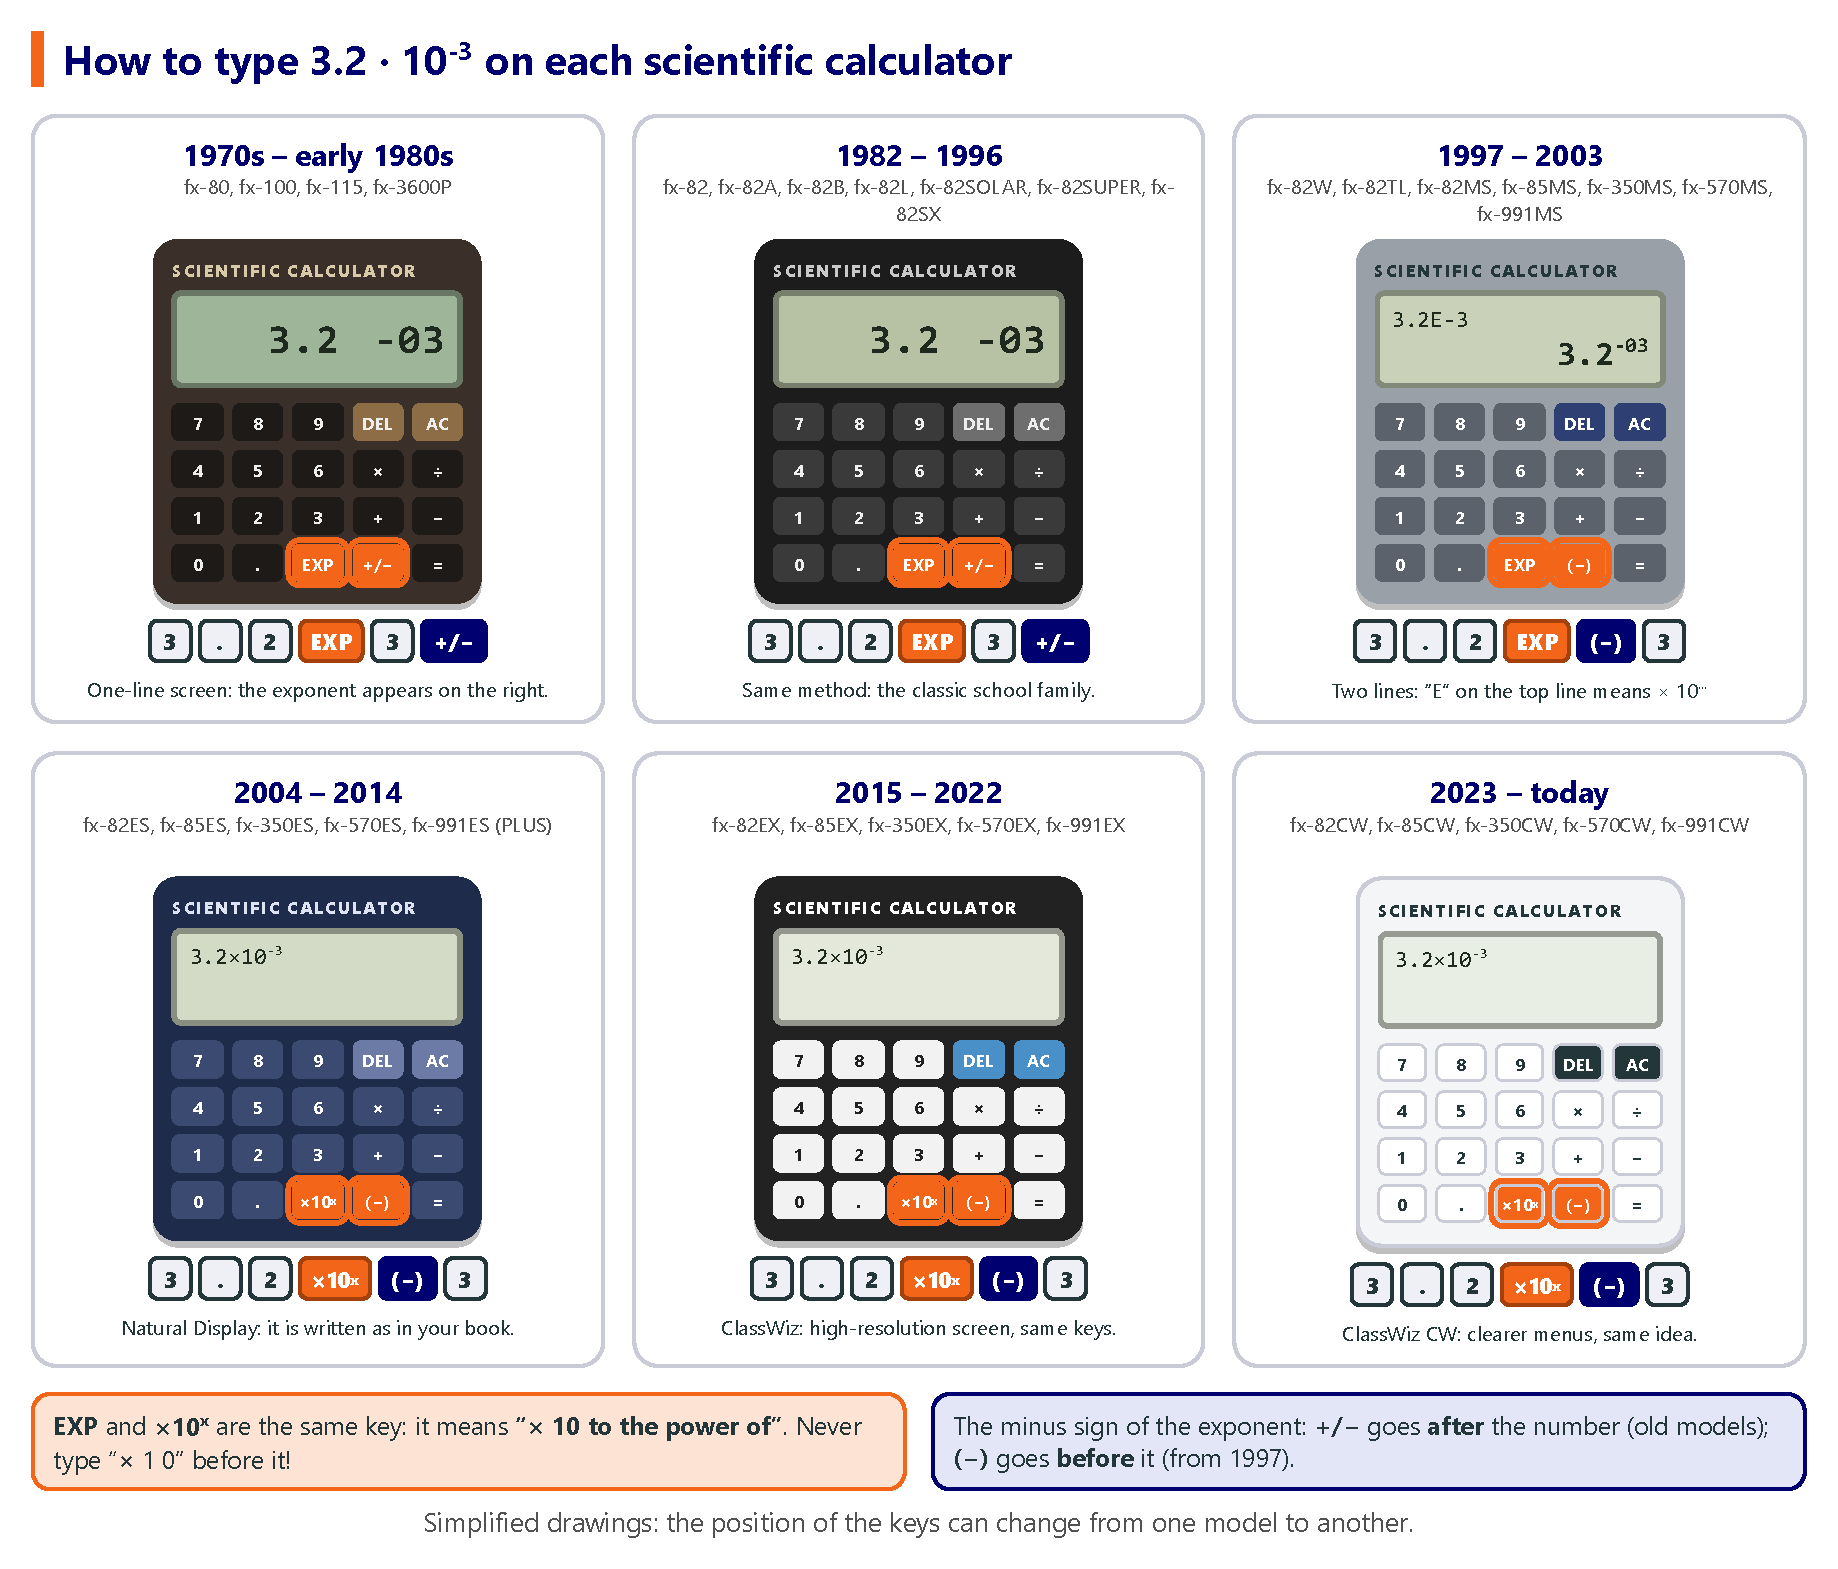
\includegraphics[width=\textwidth]{FigurasSVG/Unit_1_Matter_Measurement/pdf/calculators_sci.pdf}
    \caption{How to type \(\num{3.2e-3}\) on the scientific calculators used in schools over the years (simplified drawings).}
    \label{fig:u1_calculators_sci}
\end{figure}

\begin{table}[H]
    \centering
    \small
    \renewcommand{\arraystretch}{1.35}
    \begin{tabular}{p{1.9cm}p{4.0cm}p{2.9cm}p{3.7cm}}
        \toprule
        \textbf{Years} & \textbf{Most common models} & \textbf{Keys} & \textbf{To type \(\num{3.2e-3}\)} \\
        \midrule
        1970s--early 1980s & fx-80, fx-100, fx-115, fx-3600P & \calckey{EXP} and \calckey{+/\(-\)} & \keys{3 . 2 EXP 3 +/-} \\
        1982--1996 & fx-82, fx-82A, fx-82B, fx-82L, fx-82SOLAR, fx-82SUPER, fx-82SX & \calckey{EXP} and \calckey{+/\(-\)} & \keys{3 . 2 EXP 3 +/-} \\
        1997--2003 & fx-82W, fx-82TL, fx-82MS, fx-85W, fx-85MS, fx-115W, fx-115MS, fx-350MS, fx-570MS, fx-991MS & \calckey{EXP} and \calckey{(\(-\))} & \keys{3 . 2 EXP (-) 3} \\
        2004--2014 & fx-82ES, fx-85ES, fx-350ES, fx-570ES, fx-991ES, fx-82ES PLUS, fx-991ES PLUS & \calckey{\(\times10^{x}\)} and \calckey{(\(-\))} & \keys{3 . 2 \(\times10^{x}\) (-) 3} \\
        2015--2022 & fx-82EX, fx-85EX, fx-350EX, fx-570EX, fx-991EX (and 2nd edition) & \calckey{\(\times10^{x}\)} and \calckey{(\(-\))} & \keys{3 . 2 \(\times10^{x}\) (-) 3} \\
        2023--today & fx-82CW, fx-85CW, fx-350CW, fx-570CW, fx-991CW & \calckey{\(\times10^{x}\)} and \calckey{(\(-\))} & \keys{3 . 2 \(\times10^{x}\) (-) 3} \\
        \bottomrule
    \end{tabular}
    \caption{The scientific-notation key on the most common school calculators.}
    \label{tab:u1_calculators}
\end{table}

\begin{example}
    \textbf{Type \(\num{6.02e23}\)} (positive exponent, so no minus sign is needed):
    \begin{itemize}
        \item Calculators up to 2003: \keys{6 . 0 2 EXP 2 3}. On the screen you will see \texttt{6.02E23} or \(6.02^{23}\).
        \item Calculators from 2004 on: \keys{6 . 0 2 \(\times10^{x}\) 2 3}. On the screen you will see \(6.02 \times 10^{23}\).
    \end{itemize}
\end{example}

\begin{marker}
    \textbf{Typical mistake}: do \textbf{not} press \keys{\(\times\) 1 0} before the EXP or \(\times 10^{x}\) key, because the key already includes the ``\(\times\,10\)''. If you type \keys{3 . 2 \(\times\) 1 0 EXP (-) 3}, the calculator understands \(3{,}2 \cdot 10 \cdot 10^{-3}\), which is 10 times bigger! In the same way, to type \(10^{5}\) alone, press \keys{1 EXP 5}, not \keys{1 0 EXP 5}.
\end{marker}

\begin{exercise}
    Write the keys you would press on \textbf{your own} calculator to type these numbers, and check them on the screen: \textbf{a)} \(\num{5.4e6}\); \textbf{b)} \(\num{7.1e-4}\); \textbf{c)} \(\num{1.6e-19}\); \textbf{d)} \(\num{3e8}\).
    \begin{solu}
        With a calculator from 2004 on (with older ones, use EXP instead of \(\times 10^{x}\); before 1997, press \(+/-\) after the exponent instead of \((-)\) before it):
        a) \keys{5 . 4 \(\times10^{x}\) 6}; b) \keys{7 . 1 \(\times10^{x}\) (-) 4}; c) \keys{1 . 6 \(\times10^{x}\) (-) 1 9}; d) \keys{3 \(\times10^{x}\) 8}.
    \end{solu}
\end{exercise}


\section{Density and floating}


\begin{definition}[Density]
    The mass contained in each unit of volume of a substance:
    \begin{equation*}
        d = \dfrac{m}{V}
    \end{equation*}
\end{definition}

\begin{figure}[H]
    \centering
    % [FIGURA ORIGINAL] \includegraphics[width=\textwidth]{Unit_1/density_cubes}
    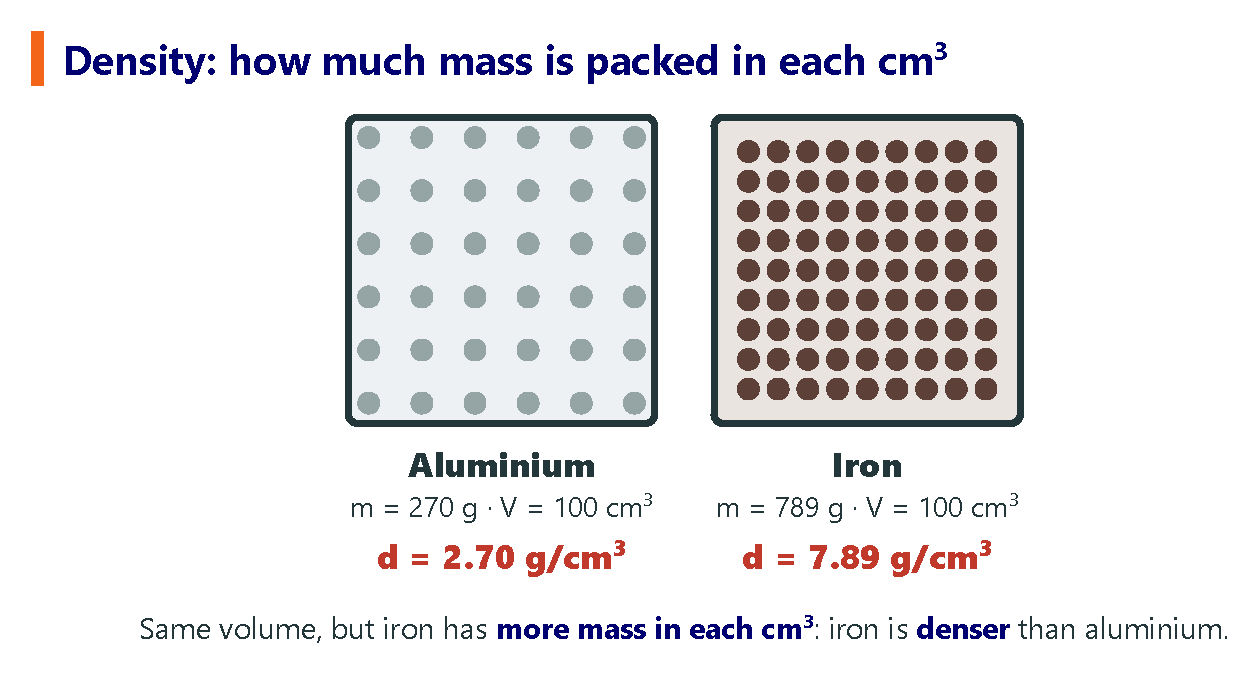
\includegraphics[width=\textwidth]{FigurasSVG/Unit_1_Matter_Measurement/pdf/density_cubes.pdf}
    \caption{Two cubes with the same volume but different mass have different densities.}
    \label{fig:u1_density_cubes}
\end{figure}

\negsubro{How to isolate a quantity in the density formula}

The formula \(d = \dfrac{m}{V}\) links three quantities. If we know \textbf{two} of them, we can always calculate the \textbf{third} one. But first we must leave the quantity we want to calculate \textbf{alone} on one side of the equals sign. This is called \textbf{isolating} (or rearranging) a quantity.

The key idea is that an equation is like a \textbf{balanced scale}: whatever we do to one side, we must also do to the other side, so that both sides stay equal.

\begin{figure}[H]
    \centering
    % [FIGURA ORIGINAL] \includegraphics[width=\textwidth]{Unit_1/density_isolate}
    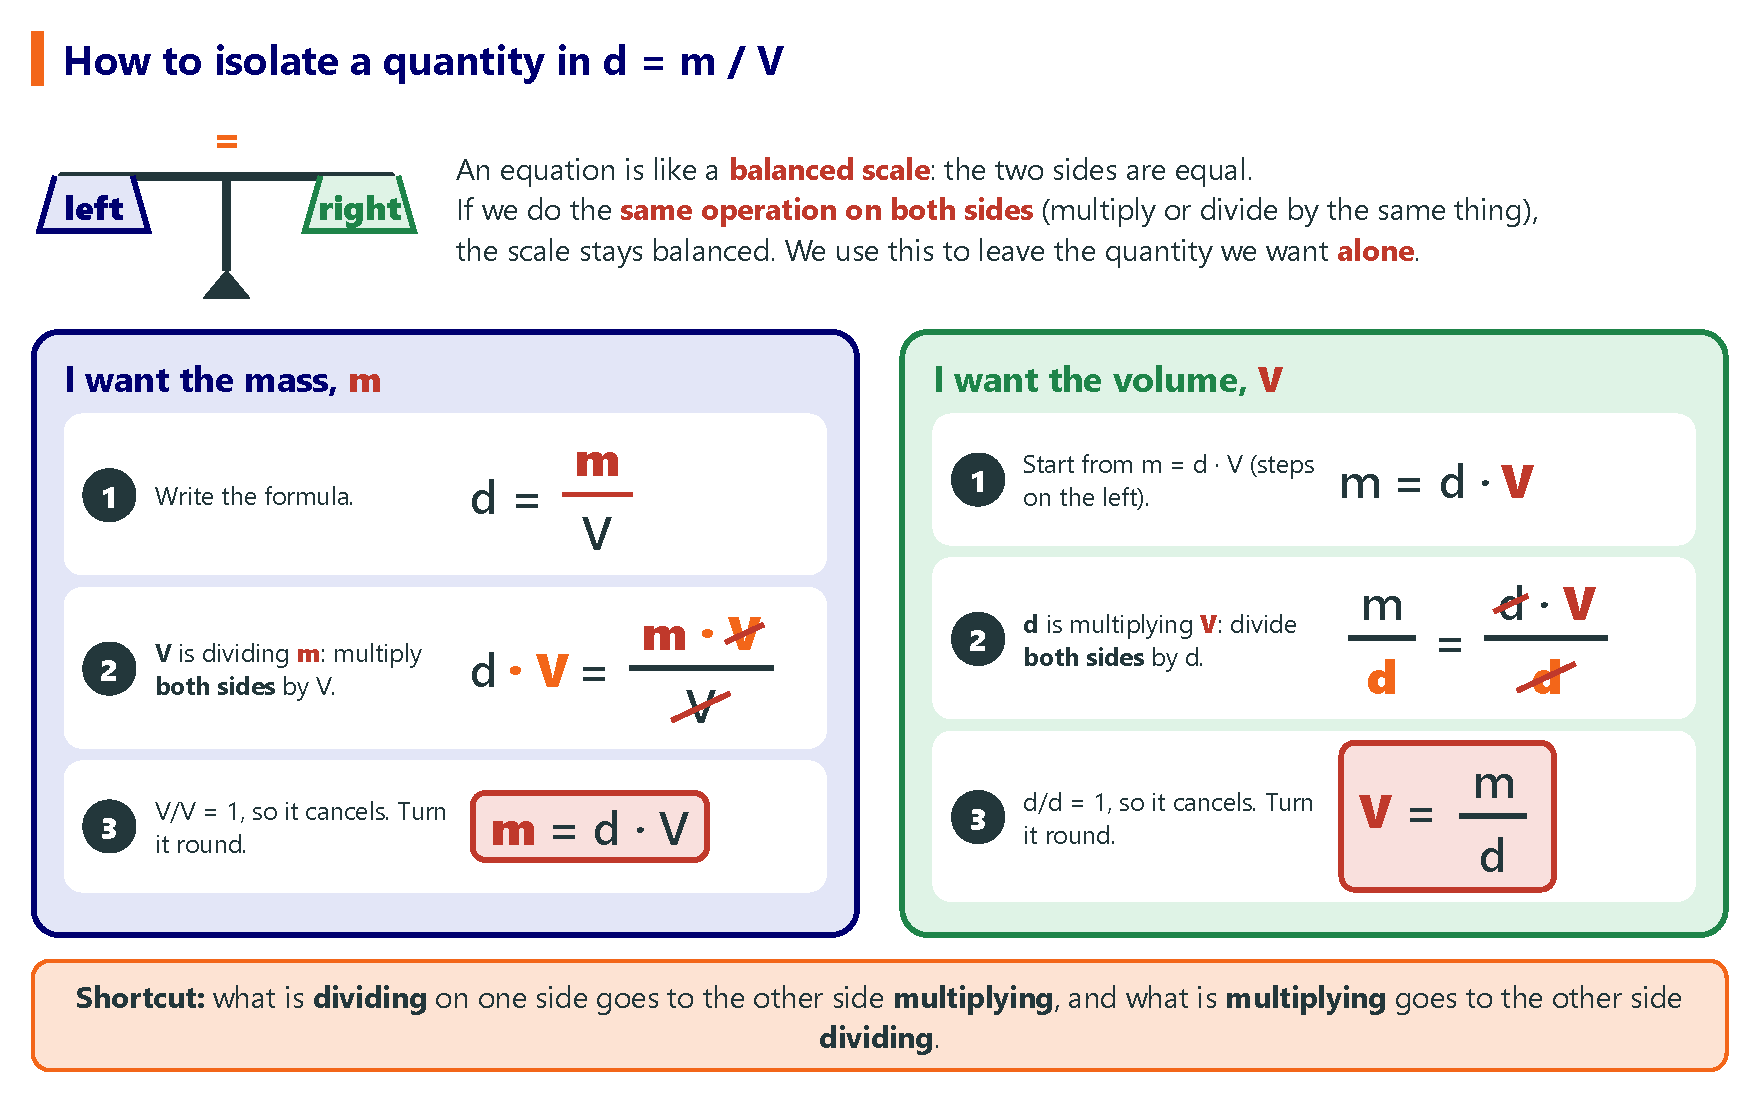
\includegraphics[width=\textwidth]{FigurasSVG/Unit_1_Matter_Measurement/pdf/density_isolate.pdf}
    \caption{Isolating the mass and the volume in the density formula, step by step.}
    \label{fig:u1_density_isolate}
\end{figure}

\negsubro{Method, step by step}:
\begin{enumerate}[label=\numberballmDarkTeal]
    \item Read the exercise and write the \textbf{data} with their units. Underline the quantity that the exercise asks for (the \textbf{unknown}).
    \item Write the formula \(d = \dfrac{m}{V}\).
    \item Look at what is \textbf{next to} the unknown and do the \textbf{opposite operation on both sides}:
    \begin{itemize}
        \item If the unknown is being \textbf{divided} by something, \textbf{multiply} both sides by it.
        \item If the unknown is being \textbf{multiplied} by something, \textbf{divide} both sides by it.
    \end{itemize}
    \item Cancel what is repeated above and below (it is worth 1) and write the unknown on the left: \(m = d \cdot V\) or \(V = \dfrac{m}{d}\).
    \item Substitute the numbers \textbf{with their units}, calculate and check that the unit of the result makes sense.
\end{enumerate}

\begin{impt}
    The three versions of the same formula:
    \begin{equation*}
        d = \dfrac{m}{V} \qquad\qquad m = d \cdot V \qquad\qquad V = \dfrac{m}{d}
    \end{equation*}
    \textbf{Shortcut}: what is \textbf{dividing} on one side goes to the other side \textbf{multiplying}, and what is \textbf{multiplying} goes to the other side \textbf{dividing}.
\end{impt}

\begin{example}
    \textbf{Calculating a mass.} A gold ring has a volume of \qty{0.8}{\cubic\cm}. The density of gold is \qty{19.3}{\g\per\cubic\cm}. What is the mass of the ring?
    \begin{enumerate}[label=\numberballmDarkTeal]
        \item Data: \(V = \qty{0.8}{\cubic\cm}\), \(d = \qty{19.3}{\g\per\cubic\cm}\). Unknown: \(\underline{m}\).
        \item Formula: \(d = \dfrac{m}{V}\).
        \item \(m\) is being divided by \(V\), so we multiply both sides by \(V\):
        \(\;d \cdot V = \dfrac{m \cdot \cancelred{V}}{\cancelred{V}}\)
        \item \(m = d \cdot V\)
        \item \(m = \qty{19.3}{\g\per\cubic\cm} \cdot \qty{0.8}{\cubic\cm} = \textcolor{red}{\qty{15.44}{\g}}\)
    \end{enumerate}
\end{example}

\begin{example}
    \textbf{Calculating a volume.} We want to pour \qty{500}{\g} of olive oil into a jug. The density of olive oil is \qty{0.92}{\g\per\mL}. What volume of oil is that?
    \begin{enumerate}[label=\numberballmDarkTeal]
        \item Data: \(m = \qty{500}{\g}\), \(d = \qty{0.92}{\g\per\mL}\). Unknown: \(\underline{V}\).
        \item Formula: \(d = \dfrac{m}{V}\). First we take \(V\) up (it is dividing, so it goes to the other side multiplying): \(m = d \cdot V\).
        \item \(V\) is being multiplied by \(d\), so we divide both sides by \(d\):
        \(\;\dfrac{m}{d} = \dfrac{\cancelred{d} \cdot V}{\cancelred{d}}\)
        \item \(V = \dfrac{m}{d}\)
        \item \(V = \dfrac{\qty{500}{\g}}{\qty{0.92}{\g\per\mL}} \approx \textcolor{red}{\qty{543}{\mL}}\)
    \end{enumerate}
\end{example}

\begin{exercise}
    Isolate the unknown and calculate:
    \begin{enumerate}[label=\letraminuscula]
        \item The mass of \qty{250}{\mL} of milk (\(d = \qty{1.03}{\g\per\mL}\)).
        \item The volume of \qty{100}{\g} of mercury (\(d = \qty{13.6}{\g\per\mL}\)).
        \item The mass of an ice cube of \qty{30}{\cubic\cm} (\(d = \qty{0.92}{\g\per\cubic\cm}\)).
        \item The volume of an aluminium piece of \qty{54}{\g} (\(d = \qty{2.70}{\g\per\cubic\cm}\)).
    \end{enumerate}
    \begin{solu}
        \begin{enumerate}[label=\alph*)]
            \item \(m = d \cdot V = \qty{1.03}{\g\per\mL} \cdot \qty{250}{\mL} = \qty{257.5}{\g}\)
            \item \(V = \dfrac{m}{d} = \dfrac{\qty{100}{\g}}{\qty{13.6}{\g\per\mL}} \approx \qty{7.35}{\mL}\)
            \item \(m = d \cdot V = \qty{0.92}{\g\per\cubic\cm} \cdot \qty{30}{\cubic\cm} = \qty{27.6}{\g}\)
            \item \(V = \dfrac{m}{d} = \dfrac{\qty{54}{\g}}{\qty{2.70}{\g\per\cubic\cm}} = \qty{20}{\cubic\cm}\)
        \end{enumerate}
    \end{solu}
\end{exercise}

\begin{exercise}
    The same method works with any formula of the type \(a = \dfrac{b}{c}\). The speed of a cyclist is \(v = \dfrac{s}{t}\), where \(s\) is the distance and \(t\) the time.
    \begin{enumerate}[label=\letraminuscula]
        \item Isolate \(s\) and \(t\), explaining the operation you do in each step.
        \item A cyclist rides at \qty{5}{\m\per\s} for \qty{120}{\s}. What distance does she cover?
        \item How long does it take her to cover \qty{1500}{\m} at the same speed?
    \end{enumerate}
    \begin{solu}
        \begin{enumerate}[label=\alph*)]
            \item \(s\) is divided by \(t\): we multiply both sides by \(t\) \(\to\) \(s = v \cdot t\). Then \(t\) is multiplied by \(v\): we divide both sides by \(v\) \(\to\) \(t = \dfrac{s}{v}\).
            \item \(s = v \cdot t = \qty{5}{\m\per\s} \cdot \qty{120}{\s} = \qty{600}{\m}\)
            \item \(t = \dfrac{s}{v} = \dfrac{\qty{1500}{\m}}{\qty{5}{\m\per\s}} = \qty{300}{\s}\)
        \end{enumerate}
    \end{solu}
\end{exercise}

\begin{exercise}
    A glass contains \qty{50}{\cmcubicos} of oil and \qty{120}{\cmcubicos} of water at \qty{20}{\celsius}. Oil is yellow, does not dissolve in water and floats because its density (\qty{0.9}{\g\per\mL}) is lower than that of water (\qty{1.0}{\g\per\mL}).
    \begin{enumerate}[label=\letraminuscula]
        \item List all the properties of matter mentioned in the text.
        \item Classify each property as quantitative/qualitative and as extensive/intensive.
    \end{enumerate}
    \begin{solu}
        \begin{enumerate}[label=\alph*)]
            \item Volume of oil, volume of water, colour of oil, solubility of oil in water, density of oil, density of water, temperature.
            \item Volumes: \textbf{quantitative, extensive}. Temperature: \textbf{quantitative, intensive}. Colour: \textbf{qualitative, intensive}. Solubility and density: \textbf{quantitative, intensive} (characteristic properties).
        \end{enumerate}
    \end{solu}
\end{exercise}

\begin{exercise}
    Match each object with the property most commonly used to choose it: copper wire, steel saucepan, cork stopper, cocoa powder, antifreeze liquid \(\;\to\;\) electrical conductivity, melting point, density, solubility in milk, thermal conductivity.
    \begin{solu}
        Copper wire \(\to\) electrical conductivity. \\
        Steel saucepan \(\to\) thermal conductivity. \\
        Cork stopper \(\to\) density. \\
        Cocoa powder \(\to\) solubility in milk. \\
        Antifreeze liquid \(\to\) melting point.
    \end{solu}
\end{exercise}

\begin{exercise}
    Classify each property as \textbf{general} or \textbf{characteristic}, and explain your reasoning: mass, boiling point, volume, hardness, temperature, density.
    \begin{solu}
        \textbf{General}: mass, volume, temperature (any type of matter can have any value, so they do not identify a substance). \\
        \textbf{Characteristic}: boiling point, hardness, density (each substance has its own value, so they can be used to identify it).
    \end{solu}
\end{exercise}

\begin{exercise}
    Two identical-looking metal cubes have masses of \qty{270}{\g} and \qty{789}{\g}, but both have a volume of \qty{100}{\cubic\cm}.
    \begin{enumerate}[label=\letraminuscula]
        \item Are mass and volume enough to tell us if the two cubes are made of the same metal? Explain.
        \item Calculate the density of each cube. Are they the same metal?
    \end{enumerate}
    \begin{solu}
        \begin{enumerate}[label=\alph*)]
            \item No, because mass and volume are \textbf{general (extensive)} properties: two different substances can have the same mass or the same volume.
            \item \(d_1 = \dfrac{\qty{270}{\g}}{\qty{100}{\mL}} = \qty{2.70}{\g\per\mL}\) (aluminium); \(d_2 = \dfrac{\qty{789}{\g}}{\qty{100}{\mL}} = \qty{7.89}{\g\per\mL}\) (iron). The densities are different, so \textbf{they are not the same metal}.
        \end{enumerate}
    \end{solu}
\end{exercise}

\begin{exercise}
    Write the data, isolate the unknown and calculate:
    \begin{enumerate}[label=\letraminuscula]
        \item A marble has a mass of \qty{5}{\g} and a volume of \qty{2}{\cubic\cm}. Calculate the density of the marble, in \unit{\g\per\cubic\cm}.
        \item A block of wood has a density of \qty{0.75}{\g\per\cubic\cm} and a volume of \qty{120}{\cubic\cm}. Calculate the mass of the block of wood, in grams.
        \item A brick has a density of \qty{500}{\kg\per\cubic\m} and a mass of \qty{10.5}{\kg}. Calculate the volume of the brick, in \unit{\cubic\m}.
        \item A metal rod has a mass of \qty{150}{\g} and a volume of \qty{25}{\cubic\cm}. Calculate the density of the rod, in \unit{\g\per\cubic\cm}.
        \item A piece of aluminium has a density of \qty{2.6}{\g\per\cubic\cm} and a volume of \qty{15}{\cubic\cm}. Calculate the mass of the aluminium, in grams.
        \item A piece of carbon has a density of \qty{2.2}{\g\per\cubic\cm} and a volume of \qty{70}{\cubic\cm}. Calculate the mass of the piece of carbon, in grams.
        \item A cube has a side length of \qty{8}{\cm} and a mass of \qty{960}{\g}. Calculate the density of the cube, in \unit{\g\per\cubic\cm}.
    \end{enumerate}
    \begin{solu}
        \begin{enumerate}[label=\alph*)]
            \item \(d = \dfrac{m}{V} = \dfrac{\qty{5}{\g}}{\qty{2}{\cubic\cm}} = \qty{2.5}{\g\per\cubic\cm}\)
            \item \(m = d \cdot V = \qty{0.75}{\g\per\cubic\cm} \cdot \qty{120}{\cubic\cm} = \qty{90}{\g}\)
            \item \(V = \dfrac{m}{d} = \dfrac{\qty{10.5}{\kg}}{\qty{500}{\kg\per\cubic\m}} = \qty{0.021}{\cubic\m} = \qty{2.1e-2}{\cubic\m}\)
            \item \(d = \dfrac{m}{V} = \dfrac{\qty{150}{\g}}{\qty{25}{\cubic\cm}} = \qty{6}{\g\per\cubic\cm}\)
            \item \(m = d \cdot V = \qty{2.6}{\g\per\cubic\cm} \cdot \qty{15}{\cubic\cm} = \qty{39}{\g}\)
            \item \(m = d \cdot V = \qty{2.2}{\g\per\cubic\cm} \cdot \qty{70}{\cubic\cm} = \qty{154}{\g}\)
            \item First the volume of the cube: \(V = \qty{8}{\cm} \cdot \qty{8}{\cm} \cdot \qty{8}{\cm} = \qty{512}{\cubic\cm}\). \\
            \(d = \dfrac{m}{V} = \dfrac{\qty{960}{\g}}{\qty{512}{\cubic\cm}} \approx \qty{1.88}{\g\per\cubic\cm}\)
        \end{enumerate}
    \end{solu}
\end{exercise}



\begin{figure}[H]
    \centering
    % [FIGURA ORIGINAL] \includegraphics[width=0.95\textwidth]{Unit_1/density_column}
    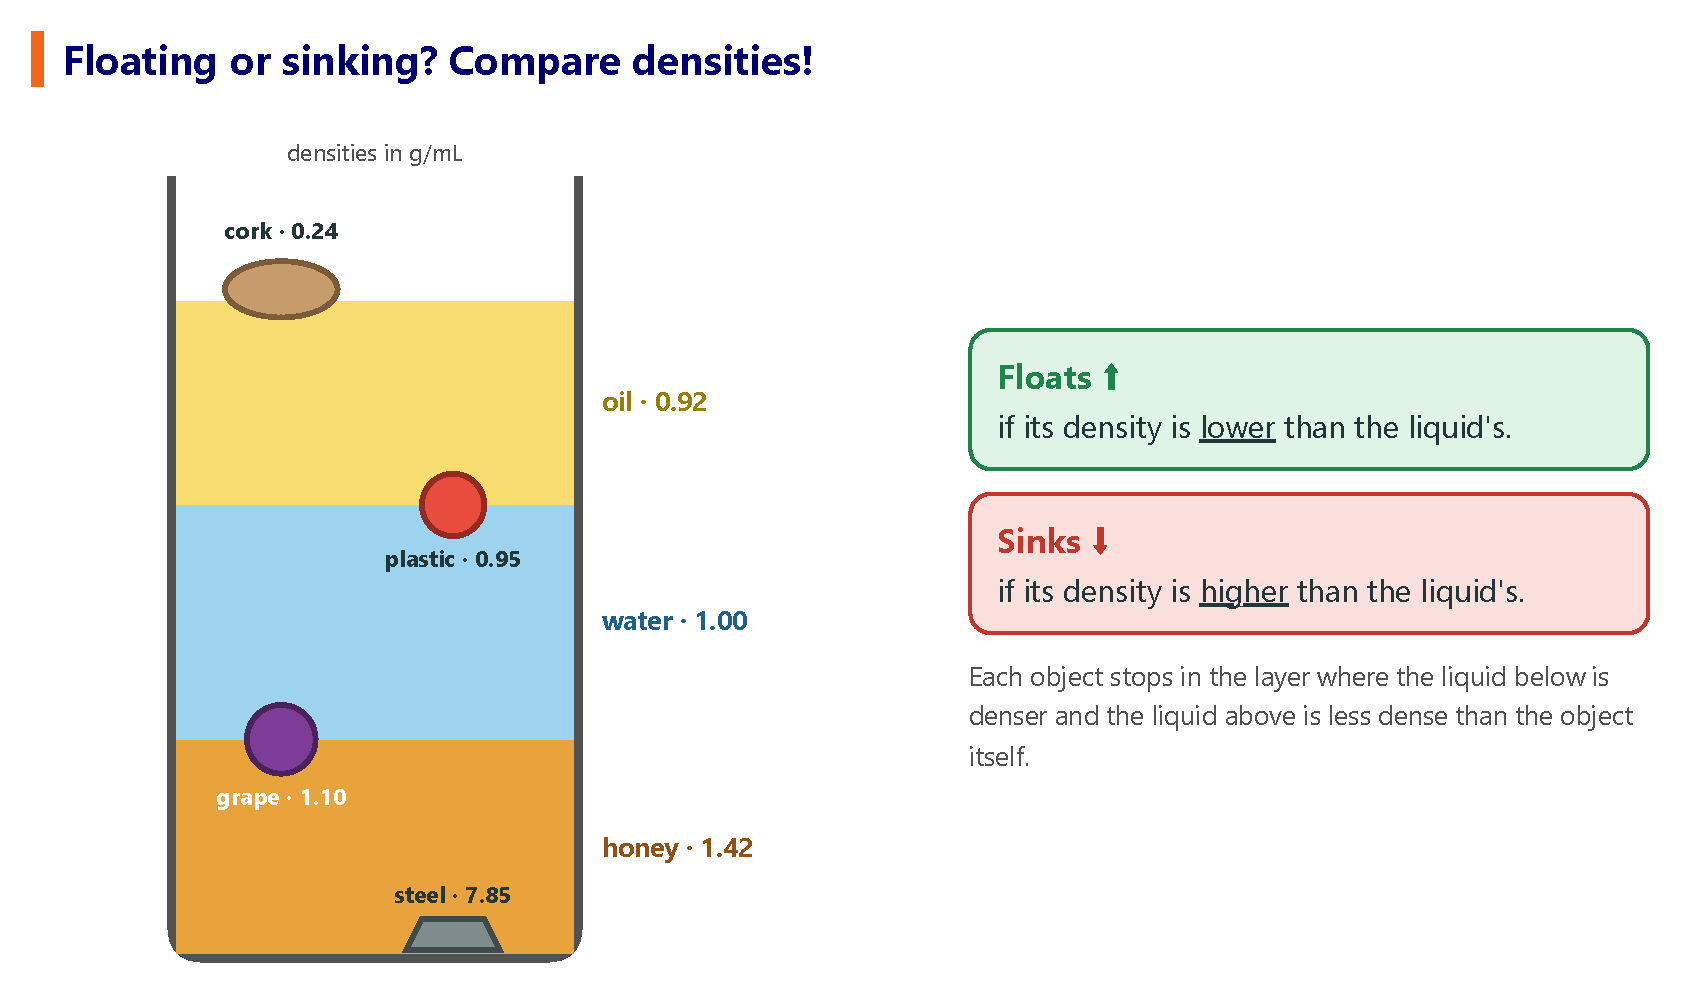
\includegraphics[width=0.95\textwidth]{FigurasSVG/Unit_1_Matter_Measurement/pdf/density_column.pdf}
    \caption{A density column: each object floats or sinks depending on its density.}
    \label{fig:u1_density_column}
\end{figure}

\begin{impt}
    In water (\(d = \qty{1.00}{\g\per\mL}\)):
    \begin{itemize}
        \item \(d_{\text{object}} < \qty{1.00}{\g\per\mL}\) \(\to\) it \textbf{floats}.
        \item \(d_{\text{object}} > \qty{1.00}{\g\per\mL}\) \(\to\) it \textbf{sinks}.
    \end{itemize}
\end{impt}

\begin{didyouknow}
    Ice (\qty{0.92}{\g\per\mL}) is less dense than liquid water, so icebergs float\ldots{} but about \textbf{90\,\%} of an iceberg is hidden under the surface. That is where the expression ``the tip of the iceberg'' comes from!
\end{didyouknow}

\begin{exercise}
    The densities of cork, aluminium and glycerin are \qty{0.24}{\g\per\mL}, \qty{2.70}{\g\per\mL} and \qty{1.26}{\g\per\mL}, respectively.
    \begin{enumerate}[label=\letraminuscula]
        \item Which of them float in water (\(d = \qty{1.00}{\g\per\mL}\))?
        \item Mercury has a density of \qty{13.6}{\g\per\mL}. Which of the three materials would float on mercury?
    \end{enumerate}
    \begin{solu}
        \begin{enumerate}[label=\alph*)]
            \item Cork floats in water (\(0.24 < 1.00\)). Aluminium and glycerin sink (\(2.70 > 1.00\) and \(1.26 > 1.00\)).
            \item All three have a density lower than mercury's, so \textbf{cork, aluminium and glycerin would all float on mercury}.
        \end{enumerate}
    \end{solu}
\end{exercise}

\begin{exercise}
    A wooden block has a mass of \qty{45}{\g} and a volume of \qty{60}{\cubic\cm}.
    \begin{enumerate}[label=\letraminuscula]
        \item Calculate its density.
        \item Will it float or sink in water? Justify your answer.
    \end{enumerate}
    \begin{solu}
        \begin{enumerate}[label=\alph*)]
            \item \(d = \dfrac{m}{V} = \dfrac{\qty{45}{\g}}{\qty{60}{\cubic\cm}} = \qty{0.75}{\g\per\cubic\cm}\).
            \item Since \(\qty{0.75}{\g\per\mL} < \qty{1.00}{\g\per\mL}\) (water), the block \textbf{floats}.
        \end{enumerate}
    \end{solu}
\end{exercise}

\begin{exercise}
    A ship is made of steel, which has a density of about \qty{7.85}{\g\per\mL}, much higher than water's. Explain, using the idea of density, why a solid steel block sinks but a steel ship floats.
    \begin{solu}
        A ship is mostly hollow (full of air), so its total volume is much larger than that of a solid steel block of the same mass. This makes the \textbf{average density of the whole ship} lower than that of water, so it floats, even though steel itself is denser than water.
    \end{solu}
\end{exercise}


%----------------------------------------------------------------------------------------

\section{Measuring instruments}

\subsection{Measuring mass}

\begin{figure}[H]
    \centering
    % [FIGURA ORIGINAL] \includegraphics[width=\textwidth]{Unit_1/balances}
    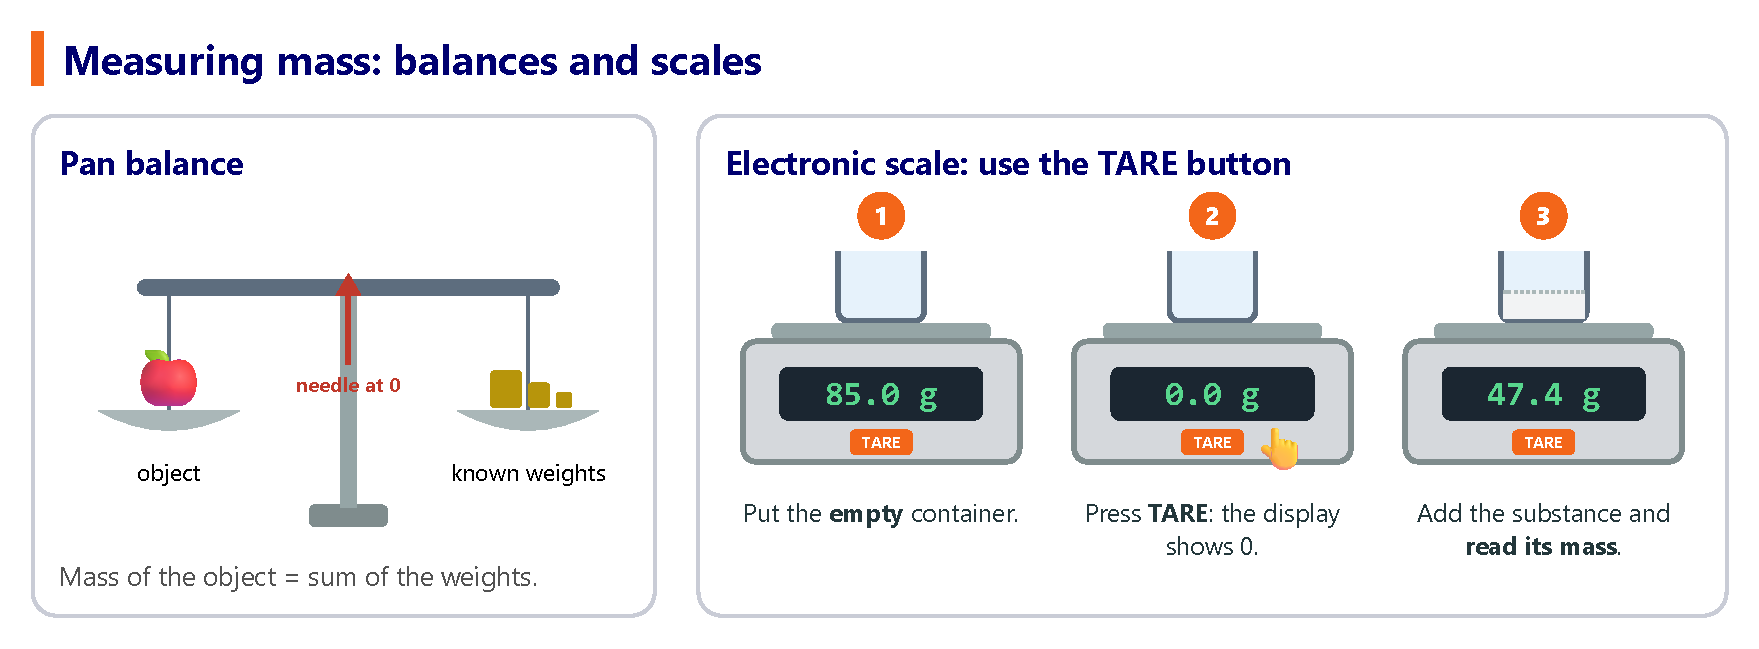
\includegraphics[width=\textwidth]{FigurasSVG/Unit_1_Matter_Measurement/pdf/balances.pdf}
    \caption{A pan balance and an electronic scale with its TARE button.}
    \label{fig:u1_balances}
\end{figure}

\begin{itemize}
    \item \negsubro{Pan balance}: put the object on one pan and add known weights to the other until the needle points to 0. Mass of the object = sum of the weights.
    \item \negsubro{Electronic scale}: put the empty container, press \textbf{TARE} (the display shows 0) and add the substance. The display shows only the mass of the substance.
\end{itemize}

\begin{impt}
    \negsubro{Mass is not weight}. \textbf{Mass} is the amount of matter (\unit{\kg}) and it is the same everywhere. \textbf{Weight} is the force with which a planet pulls a body (\unit{\N}): on the Moon you would weigh six times less, but your mass would not change.
\end{impt}

\begin{exercise}
    Explain why we press ``tare'' before adding a substance to an electronic scale, instead of simply weighing the container with the substance inside and subtracting by hand.
    \begin{solu}
        Pressing ``tare'' resets the display to zero with the empty container already on the scale, so the mass shown afterwards is directly the mass of the substance alone. This saves time and prevents calculation mistakes.
    \end{solu}
\end{exercise}

\begin{exercise}
    A student places an empty beaker on an electronic scale without pressing tare: it reads \qty{85.0}{\g}. They then add some salt, and the scale now reads \qty{132.4}{\g}.
    \begin{enumerate}[label=\letraminuscula]
        \item Calculate the mass of the salt.
        \item Explain how using ``tare'' would have made this measurement more direct.
    \end{enumerate}
    \begin{solu}
        \begin{enumerate}[label=\alph*)]
            \item Mass of salt \(= \qty{132.4}{\g} - \qty{85.0}{\g} = \qty{47.4}{\g}\).
            \item With tare, the scale would have read \qty{0}{\g} with the empty beaker, so the final reading would have been directly \qty{47.4}{\g}.
        \end{enumerate}
    \end{solu}
\end{exercise}

\subsection{Measuring volume}

\begin{itemize}
    \item \negsubro{Regular bodies} (cube, prism, cylinder, sphere\ldots): we measure their lengths and use a formula.
    \item \negsubro{Liquids and irregular bodies}: we use a \textbf{graduated cylinder}, a \textbf{burette} or a \textbf{pipette}.
\end{itemize}

\begin{definition}[Meniscus]
    The curved surface of a liquid inside a narrow tube. We read the volume at the \textbf{bottom} of the meniscus, with our eyes at the same height as the liquid.
\end{definition}

\begin{figure}[H]
    \centering
    % [FIGURA ORIGINAL] \includegraphics[width=\textwidth]{Unit_1/meniscus}
    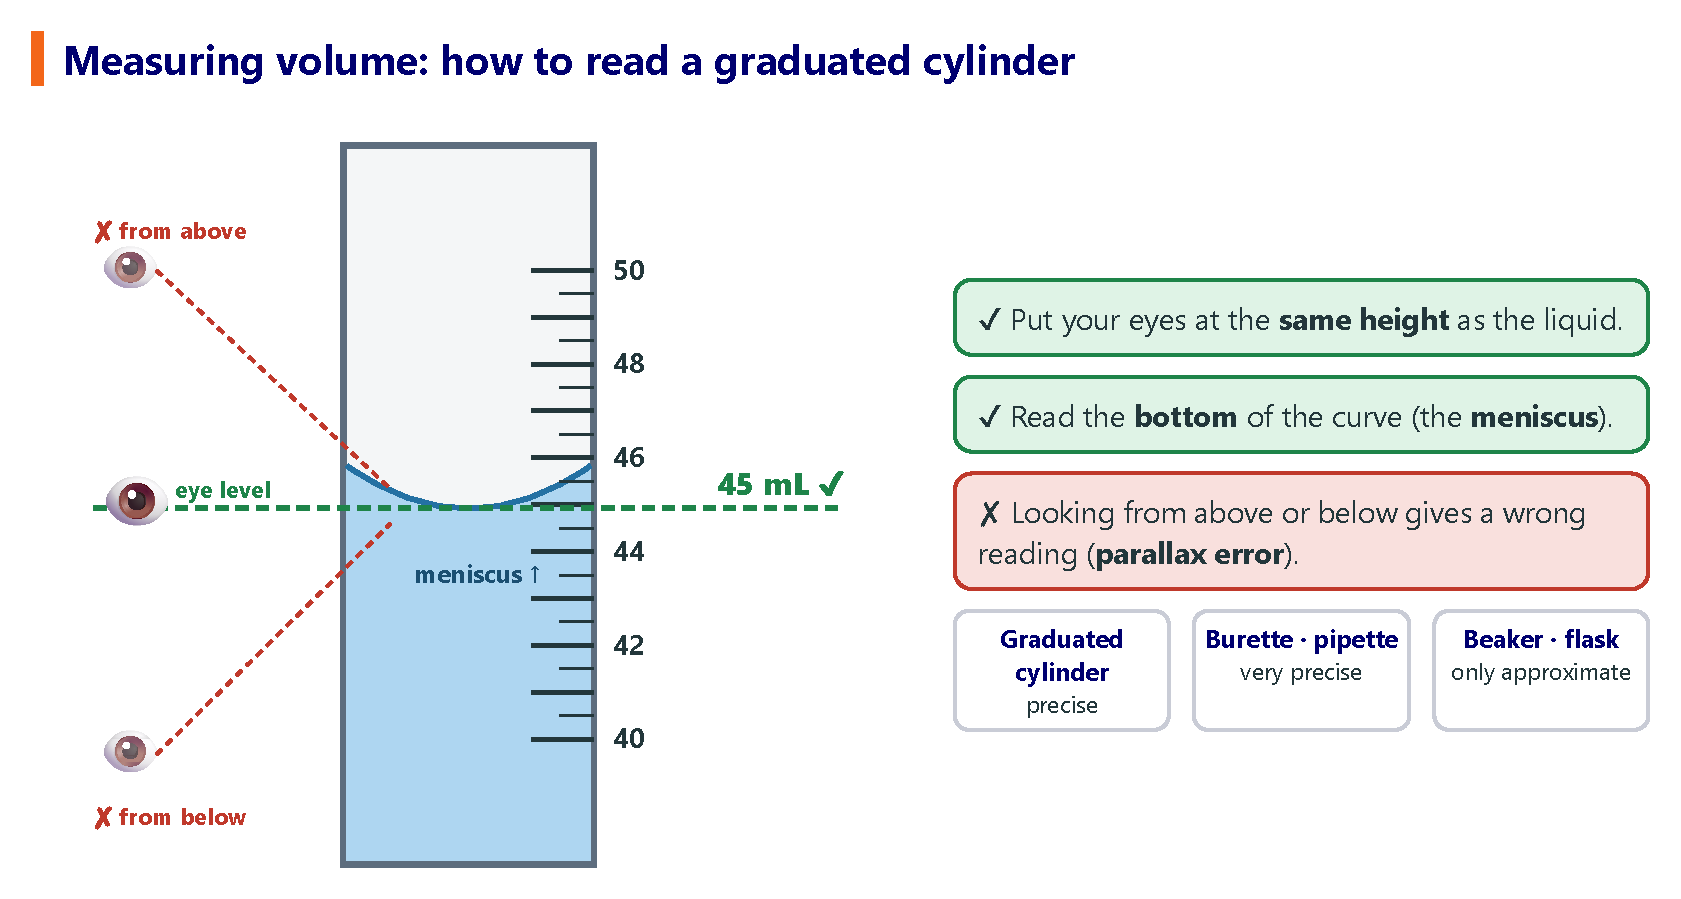
\includegraphics[width=\textwidth]{FigurasSVG/Unit_1_Matter_Measurement/pdf/meniscus.pdf}
    \caption{The correct way to read a graduated cylinder.}
    \label{fig:u1_meniscus}
\end{figure}

\begin{exercise}
    A \qty{25}{\mL} graduated cylinder allows \qty{0.5}{\mL} to be measured, and a \qty{250}{\mL} one allows \qty{5}{\mL} to be measured. Which of the two gives a more precise measurement? Why would you choose the smaller one to measure \qty{18}{\mL} of a liquid?
    \begin{solu}
        The \qty{25}{\mL} cylinder is more precise, because its smallest division (\qty{0.5}{\mL}) is smaller. \\
        For \qty{18}{\mL}, the \qty{25}{\mL} cylinder is the right choice: the liquid fills most of the cylinder and the reading is more precise.
    \end{solu}
\end{exercise}

\begin{exercise}
    Say which instrument (regular-body formula, graduated cylinder, or Erlenmeyer flask) you would use to measure the volume of each of the following, and explain why:
    \begin{enumerate}[label=\letraminuscula]
        \item A wooden cube of \qty{4}{\cm} side.
        \item \qty{35}{\mL} of vinegar for a recipe.
        \item A small, irregularly shaped stone.
        \item Roughly how much water is left in a bottle.
    \end{enumerate}
    \begin{solu}
        \begin{enumerate}[label=\alph*)]
            \item A regular body: measure the side with a ruler and use \(V = \text{side}^3\).
            \item A graduated cylinder, because it gives a precise reading of a liquid's volume.
            \item A graduated cylinder, using the rise in the water level, since the stone is irregular.
            \item An Erlenmeyer flask or beaker, since only an approximate volume is needed.
        \end{enumerate}
    \end{solu}
\end{exercise}

\begin{exercise}
    When reading the volume of water in a graduated cylinder, why must we place our eyes at the same height as the liquid's surface, and why do we read the \textbf{bottom} of the meniscus and not the top?
    \begin{solu}
        If we look from above or below, the reading is too high or too low (\textbf{parallax error}). Looking at eye level avoids this error. \\
        We read the bottom of the meniscus because water sticks to the glass walls and rises slightly at the edges; the bottom of the curve is the point that truly corresponds to the volume of liquid.
    \end{solu}
\end{exercise}

%\subsection{Precision of an instrument}
%
%\begin{definition}[Sensitivity (or appreciation) of an instrument]
%    The smallest amount that an instrument can measure: the value of its \textbf{smallest division}.
%\end{definition}
%
%\begin{figure}[H]
%    \centering
%    \includegraphics[width=\textwidth]{Unit_1/sensitivity_rulers}
%    \caption{The smaller the sensitivity, the more precise the measurement.}
%    \label{fig:u1_sensitivity_rulers}
%\end{figure}
%
%\begin{definition}[Precision and accuracy]
%    A measurement is \textbf{precise} when repeating it gives very similar values, and \textbf{accurate} when it is close to the real value. A badly calibrated instrument can be precise but not accurate.
%\end{definition}
%
%\begin{figure}[H]
%    \centering
%    \includegraphics[width=\textwidth]{Unit_1/precision_accuracy}
%    \caption{Precision and accuracy explained with a target.}
%    \label{fig:u1_precision_accuracy}
%\end{figure}
%
%\begin{exercise}
%    Three electronic scales show these masses for the same coin: scale A gives \qty{2.5}{\g}, scale B gives \qty{2.52}{\g} and scale C gives \qty{2.524}{\g}.
%    \begin{enumerate}[label=\letraminuscula]
%        \item Order the three scales from least to most precise.
%        \item If the coin's real mass is known to be \qty{2.50}{\g}, which of the three measurements is the most accurate?
%    \end{enumerate}
%    \begin{solu}
%        \begin{enumerate}[label=\alph*)]
%            \item From least to most precise: A (sensitivity \qty{0.1}{\g}) \(<\) B (\qty{0.01}{\g}) \(<\) C (\qty{0.001}{\g}).
%            \item Scale A's reading (\qty{2.5}{\g}) is exactly the real value, so it is the most \textbf{accurate}, even though it is the least precise.
%        \end{enumerate}
%    \end{solu}
%\end{exercise}
%
%\begin{exercise}
%    A ruler has millimetre divisions, and a tape measure used in a workshop has only centimetre divisions.
%    \begin{enumerate}[label=\letraminuscula]
%        \item What is the sensitivity of each instrument?
%        \item Which one would you use to measure the length of a pencil as precisely as possible? Explain.
%    \end{enumerate}
%    \begin{solu}
%        \begin{enumerate}[label=\alph*)]
%            \item Ruler: \qty{1}{\mm}. Tape measure: \qty{1}{\cm}.
%            \item The \textbf{ruler}, because its sensitivity is smaller (\(\qty{1}{\mm} < \qty{1}{\cm}\)), so it allows a more precise reading.
%        \end{enumerate}
%    \end{solu}
%\end{exercise}
%
%\begin{exercise}
%    Four archers shoot four arrows each at a target. Archer 1's arrows all land close together, but far from the bullseye. Archer 2's arrows land scattered all around the target. Archer 3's arrows all land close together, right on the bullseye. Archer 4's arrows land scattered but roughly centred on the bullseye.
%    \begin{enumerate}[label=\letraminuscula]
%        \item Which archer represents ``precise but not accurate''?
%        \item Which archer represents ``precise and accurate''?
%    \end{enumerate}
%    \begin{solu}
%        \begin{enumerate}[label=\alph*)]
%            \item Archer 1: the arrows are close together (precise) but far from the bullseye (not accurate).
%            \item Archer 3: the arrows are close together (precise) and on the bullseye (accurate).
%        \end{enumerate}
%    \end{solu}
%\end{exercise}

%----------------------------------------------------------------------------------------

\section{Indirect measurements}

\begin{definition}[Indirect measurement]
    A measurement that we \textbf{calculate} from other quantities that we have measured directly.
\end{definition}

Mass and length can be read directly on an instrument, but surface area, density or very small thicknesses usually have to be \textbf{calculated}.

%\subsection{Measuring surface area indirectly}
%
%\begin{figure}[H]
%    \centering
%    \includegraphics[width=\textwidth]{Unit_1/indirect_area}
%    \caption{The surface of an irregular shape is proportional to its mass if the material is the same.}
%    \label{fig:u1_indirect_area}
%\end{figure}
%
%\vspace{2.5\baselineskip}
%% centered by hand: with fleqn an equation* goes to the left margin and the left labels fall off the page
%\begin{center}
%    \(\displaystyle
%        \eqnmarkbox[ochre]{u1sf}{S_F} =
%        \eqnmarkbox[signBlue]{u1sm}{S_M} \cdot
%        \dfrac{\eqnmarkbox[indigo2]{u1mf}{M_F}}{\eqnmarkbox[firebrick]{u1mm}{M_M}}
%    \)
%\end{center}
%\annotate[yshift=1.2em]{above,left}{u1sf}{Surface of the irregular figure}
%\annotate[yshift=-1.2em]{below,left}{u1sm}{Surface of the measured square}
%\annotate[yshift=1.2em]{above,right}{u1mf}{Mass of the cut-out figure}
%\annotate[yshift=-1.2em]{below,right}{u1mm}{Mass of the measured square}
%\vspace{2.5\baselineskip}
%
%\begin{exercise}
%    To find the surface area of an irregularly shaped leaf, a student cuts a square of paper of \(S_M = \qty{1}{\square\dm}\) from the same type of paper and weighs it: \(M_M = \qty{15.0}{\g}\). She then traces the leaf's outline on the same paper, cuts it out and weighs it: \(M_F = \qty{3.0}{\g}\).
%    \begin{enumerate}[label=\letraminuscula]
%        \item Calculate the surface area of the leaf.
%        \item Explain why the measured square and the leaf cut-out must be made of exactly the same paper.
%    \end{enumerate}
%    \begin{solu}
%        \begin{enumerate}[label=\alph*)]
%            \item \(S_F = S_M \cdot \dfrac{M_F}{M_M} = \qty{1}{\square\dm} \cdot \dfrac{\qty{3.0}{\g}}{\qty{15.0}{\g}} = \qty{0.20}{\square\dm}\).
%            \item The method only works if mass is proportional to surface area, which is true only if the paper has the same thickness and density everywhere.
%        \end{enumerate}
%    \end{solu}
%\end{exercise}
%
%\begin{exercise}
%    A measured square of cardboard with \(S_M = \qty{1}{\square\dm}\) has a mass of \(M_M = \qty{40}{\g}\). An irregular piece of the same cardboard has a surface area of \qty{0.65}{\square\dm}. What mass should this irregular piece have?
%    \begin{solu}
%        \(M_F = M_M \cdot \dfrac{S_F}{S_M} = \qty{40}{\g} \cdot \dfrac{\qty{0.65}{\square\dm}}{\qty{1}{\square\dm}} = \qty{26}{\g}\).
%    \end{solu}
%\end{exercise}

\subsection{Measuring density}

\begin{itemize}
    \item \negsubro{Liquid}: tare a graduated cylinder on the scale, pour in the liquid, read its volume \(V\) and its mass \(m\), and calculate \(d = m/V\).
    \item \negsubro{Solid that does not dissolve in water}: weigh it, and find its volume by \textbf{water displacement}, as shown in the figure.
\end{itemize}

\begin{figure}[H]
    \centering
    % [FIGURA ORIGINAL] \includegraphics[width=\textwidth]{Unit_1/density_lab}
    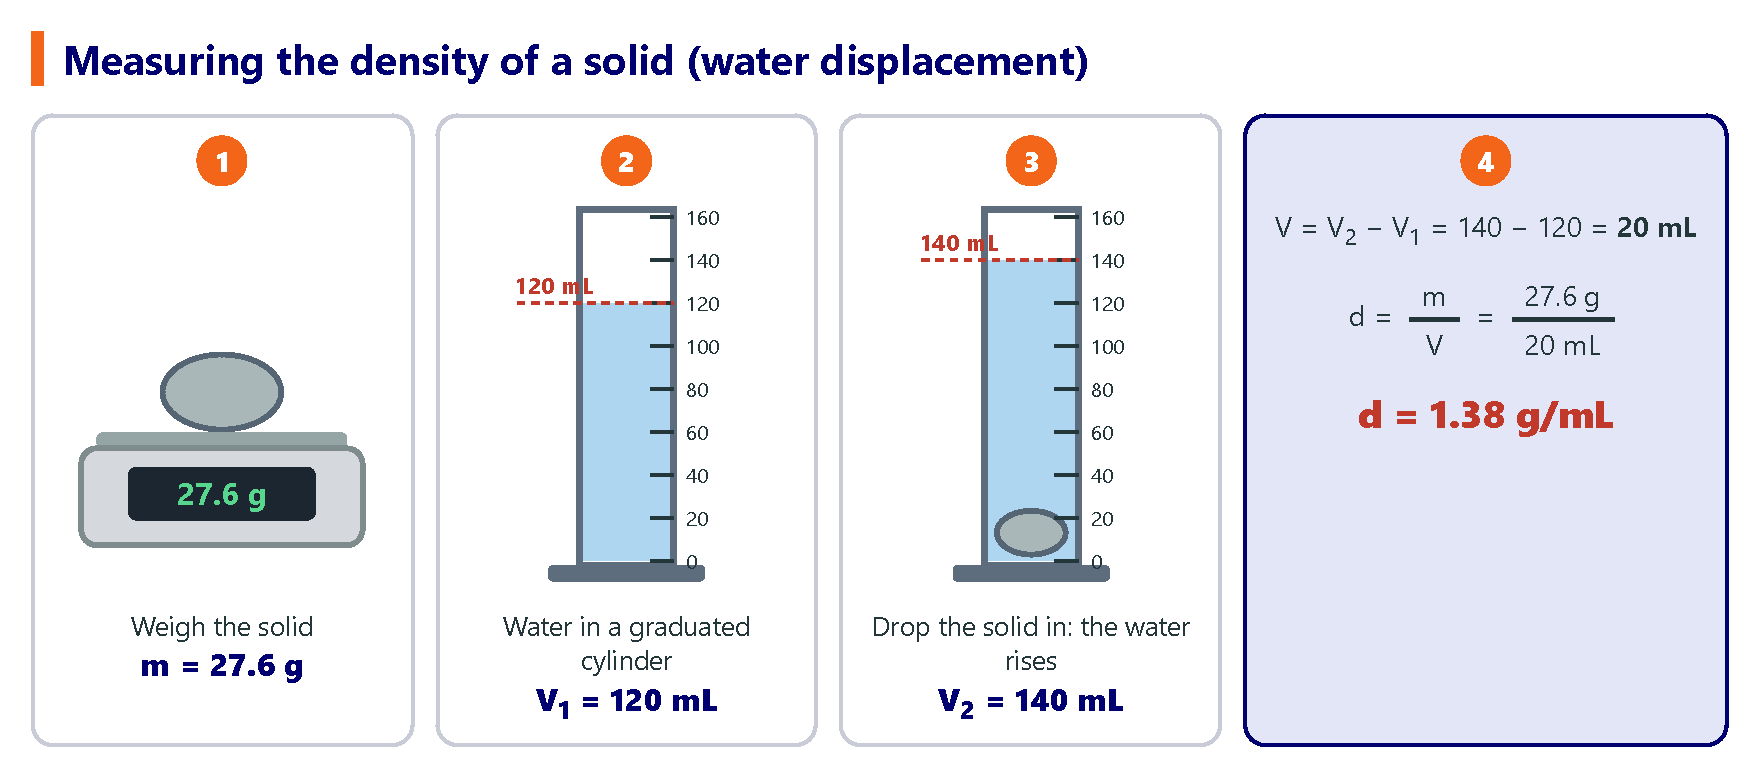
\includegraphics[width=\textwidth]{FigurasSVG/Unit_1_Matter_Measurement/pdf/density_lab.pdf}
    \caption{Measuring the density of a solid: the volume of the solid is the rise in the water level.}
    \label{fig:u1_density_lab}
\end{figure}

\begin{didyouknow}
    According to legend, Archimedes discovered this method in his bath: when he got in, the water level rose. He realised he could use it to measure the volume of the king's crown and check whether it was made of pure gold. He was so excited that he ran into the street shouting ``Eureka!'' (``I have found it!'').
\end{didyouknow}

\begin{exercise}
    A block of modelling clay has a mass of \qty{27.6}{\g}. When we put it into a graduated cylinder with \qty{120}{\mL} of water, the level rises to \qty{140}{\mL}.
    \begin{enumerate}[label=\letraminuscula]
        \item Calculate the density of the modelling clay.
        \item If a second block, made of the same clay, had half the volume, what would its mass and density be?
    \end{enumerate}
    \begin{solu}
        \begin{enumerate}[label=\alph*)]
            \item \(V = \qty{140}{\mL} - \qty{120}{\mL} = \qty{20}{\mL}\); \(d = \dfrac{\qty{27.6}{\g}}{\qty{20}{\mL}} = \qty{1.38}{\g\per\mL}\).
            \item Half the volume (\qty{10}{\mL}) means half the mass (\qty{13.8}{\g}). The \textbf{density does not change} (\qty{1.38}{\g\per\mL}), because it is a characteristic property.
        \end{enumerate}
    \end{solu}
\end{exercise}

\begin{exercise}
    To measure the density of sugar: mass of the empty graduated cylinder = \qty{130}{\g}; mass of the graduated cylinder containing the sugar = \qty{198.5}{\g}; when the sugar is poured into a cylinder with \qty{100}{\mL} of a liquid in which it does not dissolve, the level rises to \qty{130}{\mL}. What is the density of the sugar?
    \begin{solu}
        Mass of sugar \(= \qty{198.5}{\g} - \qty{130}{\g} = \qty{68.5}{\g}\). \\
        Volume of sugar \(= \qty{130}{\mL} - \qty{100}{\mL} = \qty{30}{\mL}\). \\
        Density: \(d = \dfrac{\qty{68.5}{\g}}{\qty{30}{\mL}} \approx \qty{2.28}{\g\per\mL}\).
    \end{solu}
\end{exercise}

\begin{exercise}
    The densities of milk, water and oil are \qty{1.04}{\g\per\mL}, \qty{1.00}{\g\per\mL} and \qty{0.92}{\g\per\mL}, respectively. Calculate the mass of \qty{1}{\litre} of each one.
    \begin{solu}
        Using \(m = d \cdot V\) with \(V = \qty{1000}{\mL}\): \\
        Milk: \(m = \qty{1.04}{\g\per\mL} \cdot \qty{1000}{\mL} = \qty{1040}{\g}\). \\
        Water: \(m = \qty{1000}{\g}\). \\
        Oil: \(m = \qty{920}{\g}\).
    \end{solu}
\end{exercise}

%\subsection{Measuring very small thicknesses indirectly}
%
%Some lengths are too small for a ruler, such as the thickness of a sheet of paper. The trick: measure \textbf{many} of them together and divide.
%
%\begin{figure}[H]
%    \centering
%    \includegraphics[width=\textwidth]{Unit_1/stack_thickness}
%    \caption{The thickness of one sheet is the thickness of the pile divided by the number of sheets.}
%    \label{fig:u1_stack_thickness}
%\end{figure}
%
%\begin{exercise}
%    A pile of 40 identical CD cases is \qty{36}{\cm} tall. Calculate the thickness of a single CD case, in mm.
%    \begin{solu}
%        \(e = \dfrac{\qty{36}{\cm}}{40} = \qty{0.9}{\cm} = \qty{9}{\mm}\).
%    \end{solu}
%\end{exercise}
%
%\begin{exercise}
%    A ream of 500 sheets of paper is \qty{5.5}{\cm} thick.
%    \begin{enumerate}[label=\letraminuscula]
%        \item Calculate the thickness of one sheet, in mm.
%        \item How many sheets would you need to stack to get a pile exactly \qty{1}{\cm} tall?
%    \end{enumerate}
%    \begin{solu}
%        \begin{enumerate}[label=\alph*)]
%            \item \(e = \dfrac{\qty{5.5}{\cm}}{500} = \qty{0.011}{\cm} = \qty{0.11}{\mm}\).
%            \item Number of sheets \(= \dfrac{\qty{1}{\cm}}{\qty{0.011}{\cm}} \approx 91\) sheets.
%        \end{enumerate}
%    \end{solu}
%\end{exercise}
%
%\begin{exercise}
%    Explain why we cannot measure the thickness of a single coin directly and precisely with a ruler that has millimetre divisions, and describe briefly how the indirect method solves this problem.
%    \begin{solu}
%        A coin's thickness (1--2 mm) is very close to the ruler's sensitivity (\qty{1}{\mm}), so a direct reading would have a very large error. \\
%        Stacking many coins gives a much longer length, where the error of the ruler is small in comparison. Dividing by the number of coins gives a much more precise value for one coin.
%    \end{solu}
%\end{exercise}

%----------------------------------------------------------------------------------------

\section{Laboratory equipment and safety rules}

The laboratory is where we do experiments. It is great fun\ldots{} but only if we know the material and follow the safety rules.

\subsection{Common laboratory equipment}

\begin{figure}[H]
    \centering
    
\begin{tikzpicture}[scale=0.5]
        \begin{scope}
            \tkzTestTube[glassType=tube,liquidLevel1=40]
            \node[align=center, text width=2.4cm] at (0,-1) {\small Test tube};
        \end{scope}
        \begin{scope}[xshift=5cm]
            \tkzTestTube[glassType=beaker,liquidLevel1=40]
            \node[align=center, text width=2.4cm] at (0,-1) {\small Beaker};
        \end{scope}
        \begin{scope}[xshift=10cm]
            \tkzTestTube[glassType=erlenmeyer,liquidLevel1=30]
            \node[align=center, text width=2.4cm] at (0,-1) {\small Erlenmeyer flask};
        \end{scope}
        \begin{scope}[xshift=15cm]
            \tkzGraduatedCylinder[liquidLevel1=60]
            \node[align=center, text width=2.4cm] at (0,-1) {\small Graduated cylinder};
        \end{scope}
        \begin{scope}[xshift=20.5cm]
            \tkzBunsenBurner
            \node[align=center, text width=2.4cm] at (0,-1) {\small Bunsen burner};
        \end{scope}
    \end{tikzpicture}
    \caption{Common laboratory glassware and a Bunsen burner, drawn with the \texttt{tikz-chemlab} package.}
    \label{fig:glassware}
\end{figure}

\begin{table}[H]
    \centering
    \small
    \renewcommand{\arraystretch}{1.35}
    \begin{tabular}{p{3.3cm}p{9.5cm}}
        \toprule
        \textbf{Material} & \textbf{What we use it for} \\
        \midrule
        Test tube & hold, heat or mix \textbf{small} amounts of substances \\
        Beaker & mix or heat liquids; measure \textbf{approximate} volumes \\
        Erlenmeyer flask & mix or heat liquids without spilling them (narrow neck) \\
        Graduated cylinder & measure the volume of a liquid \textbf{precisely} \\
        Bunsen burner & heat source (gas flame) \\
        \bottomrule
    \end{tabular}
    \caption{Basic laboratory material and its uses.}
    \label{tab:u1_lab_material}
\end{table}

\subsection{Safety in the laboratory}

\begin{figure}[H]
    \centering
    % [FIGURA ORIGINAL] \includegraphics[width=\textwidth]{Unit_1/lab_safety}
    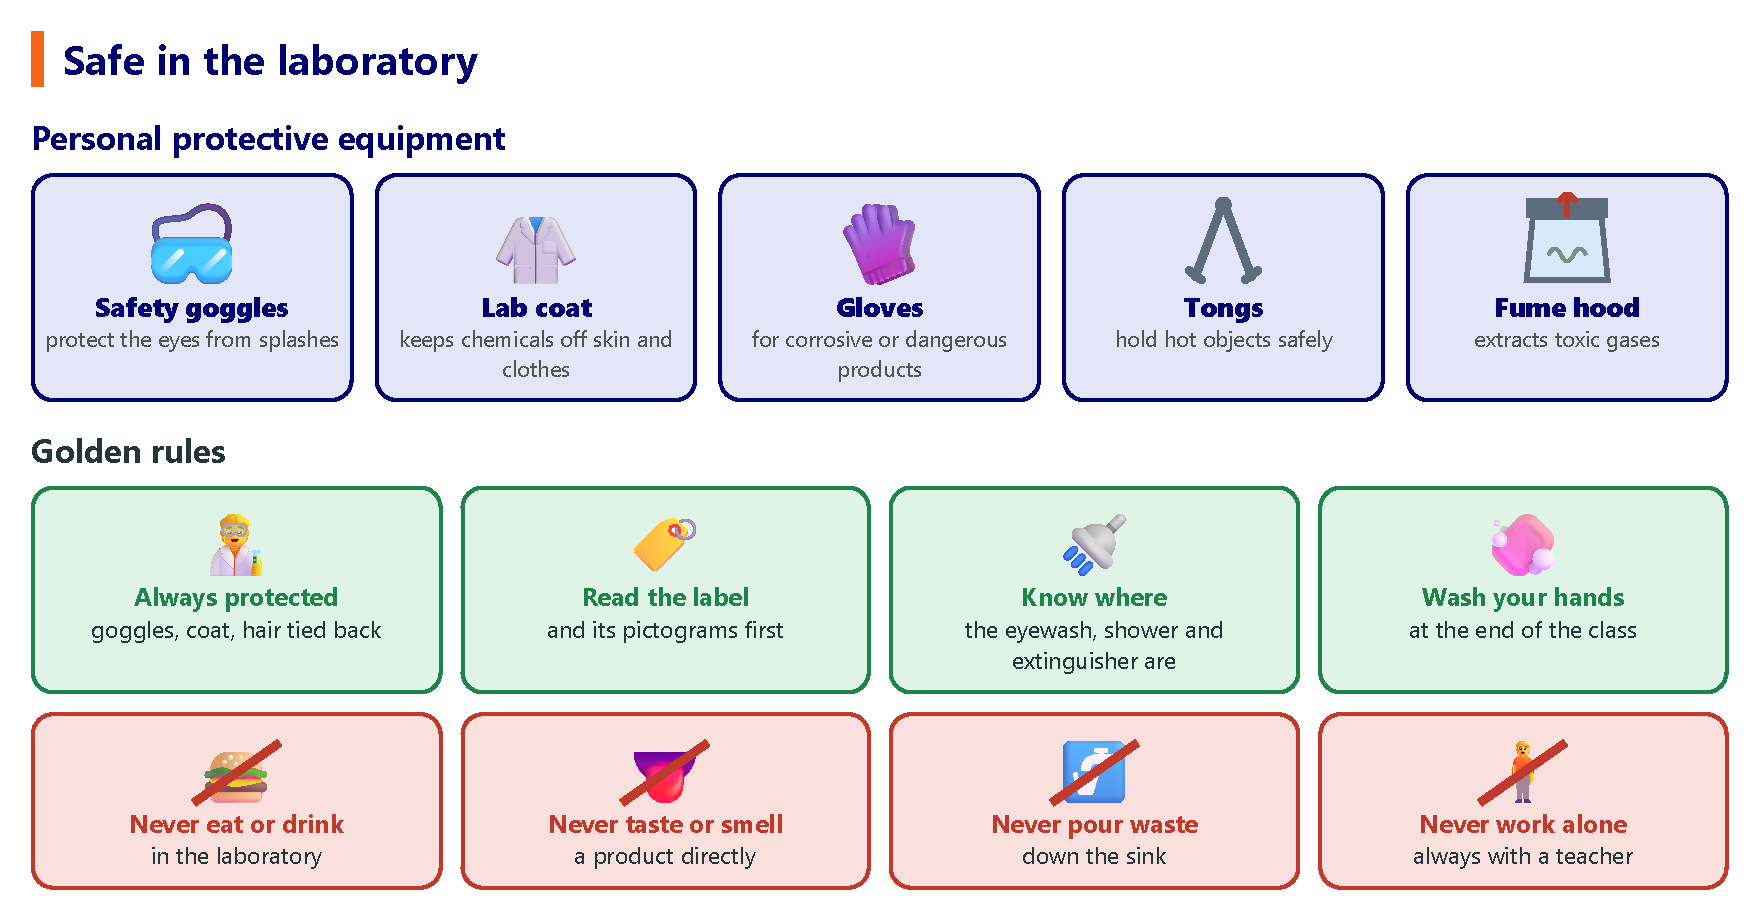
\includegraphics[width=\textwidth]{FigurasSVG/Unit_1_Matter_Measurement/pdf/lab_safety.pdf}
    \caption{Personal protective equipment and golden rules of the laboratory.}
    \label{fig:u1_lab_safety}
\end{figure}

Two more rules that are easy to forget:
\begin{enumerate}[label=\numberballmDarkTeal]
    \item Point a test tube that is being heated \textbf{away} from yourself and from other people.
    \item Keep your bench tidy, and use only the material and amounts that your teacher tells you.
\end{enumerate}

\subsection{Hazard pictograms (GHS)}

\begin{definition}[Hazard pictogram]
    A standardised symbol, black on a white background inside a red diamond, printed on the label of a chemical product to warn us, at a glance, about the type of danger it presents. The current set is fixed by the \negsubro{Globally Harmonized System (GHS)}, used all around the world.
\end{definition}

\begin{figure}[H]
    \centering
    \begin{tabular}{@{}p{5.0cm}p{5.0cm}p{5.0cm}@{}}
        \begin{minipage}{5.0cm}
            \centering
            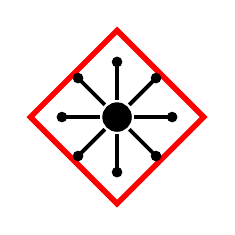
\begin{tikzpicture}
                \draw[draw=red, line width=2pt, fill=white] (0,-1.1) -- (1.1,0) -- (0,1.1) -- (-1.1,0) -- cycle;
                \filldraw[black] (0,0) circle (0.18);
                \foreach \a in {0,45,90,135,180,225,270,315}{
                    \draw[line width=1.4pt] (\a:0.22) -- (\a:0.65);
                    \filldraw[black] (\a:0.7) circle (0.06);
                }
            \end{tikzpicture}\\[2pt]
            \textbf{Explosive}\\[2pt]
            {\small Can explode with heat, shock or friction. Example: fireworks.}
        \end{minipage}
        &
        \begin{minipage}{5.0cm}
            \centering
            
\begin{tikzpicture}
                \draw[draw=red, line width=2pt, fill=white] (0,-1.1) -- (1.1,0) -- (0,1.1) -- (-1.1,0) -- cycle;
                \fill[black] plot [smooth cycle] coordinates {(0,-0.75) (0.32,-0.35) (0.22,0.05) (0.42,0.35) (0.12,0.75) (-0.15,0.35) (-0.32,0.0) (-0.18,-0.35)};
                \fill[white] plot [smooth cycle] coordinates {(0,-0.4) (0.14,-0.1) (0.05,0.15) (0.14,0.35) (0,0.55) (-0.1,0.3) (-0.14,0.0) (-0.05,-0.2)};
            \end{tikzpicture}\\[2pt]
            \textbf{Flammable}\\[2pt]
            {\small Catches fire easily. Example: alcohol, petrol.}
        \end{minipage}
        &
        \begin{minipage}{5.0cm}
            \centering
            
\begin{tikzpicture}
                \draw[draw=red, line width=2pt, fill=white] (0,-1.1) -- (1.1,0) -- (0,1.1) -- (-1.1,0) -- cycle;
                \draw[line width=1.6pt] (0,-0.85) circle (0.2);
                \begin{scope}[yshift=0.15cm]
                    \fill[black] plot [smooth cycle] coordinates {(0,-0.75) (0.32,-0.35) (0.22,0.05) (0.42,0.35) (0.12,0.75) (-0.15,0.35) (-0.32,0.0) (-0.18,-0.35)};
                \end{scope}
            \end{tikzpicture}\\[2pt]
            \textbf{Oxidizing}\\[2pt]
            {\small Feeds a fire, making it burn more strongly. Example: bleach, oxygen bottles.}
        \end{minipage}
        \\[9mm]
        \begin{minipage}{5.0cm}
            \centering
            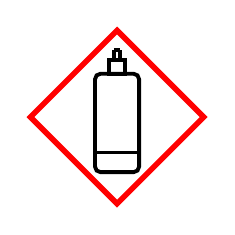
\begin{tikzpicture}
                \draw[draw=red, line width=2pt, fill=white] (0,-1.1) -- (1.1,0) -- (0,1.1) -- (-1.1,0) -- cycle;
                \draw[line width=1.4pt, rounded corners=2pt] (-0.28,-0.7) rectangle (0.28,0.55);
                \draw[line width=1.4pt] (-0.1,0.55) rectangle (0.1,0.72);
                \draw[line width=1.4pt] (-0.04,0.72) -- (-0.04,0.85);
                \draw[line width=1.4pt] (0.04,0.72) -- (0.04,0.85);
                \draw[line width=1.4pt] (-0.04,0.85) -- (0.04,0.85);
                \draw[line width=1pt] (-0.28,-0.45) -- (0.28,-0.45);
            \end{tikzpicture}\\[2pt]
            \textbf{Compressed gas}\\[2pt]
            {\small Gas stored under pressure, may explode when heated. Example: gas cylinders.}
        \end{minipage}
        &
        \begin{minipage}{5.0cm}
            \centering
            
\begin{tikzpicture}
                \draw[draw=red, line width=2pt, fill=white] (0,-1.1) -- (1.1,0) -- (0,1.1) -- (-1.1,0) -- cycle;
                \begin{scope}[rotate=20, shift={(-0.35,0.55)}]
                    \draw[line width=1.2pt] (-0.1,-0.35) -- (-0.1,0.35) arc (180:0:0.1) -- (0.1,-0.35) -- cycle;
                \end{scope}
                \begin{scope}[rotate=-20, shift={(0.35,0.55)}]
                    \draw[line width=1.2pt] (-0.1,-0.35) -- (-0.1,0.35) arc (180:0:0.1) -- (0.1,-0.35) -- cycle;
                \end{scope}
                \draw[line width=1pt] (-0.15,0.15) -- (-0.05,-0.05);
                \draw[line width=1pt] (0.15,0.15) -- (0.05,-0.05);
                \fill[black] (-0.45,-0.15) -- (0.45,-0.15) -- (0.4,-0.3) -- (0.3,-0.18) -- (0.2,-0.32) -- (0.1,-0.16) -- (0,-0.3) -- (-0.1,-0.16) -- (-0.2,-0.3) -- (-0.3,-0.16) -- (-0.4,-0.28) -- cycle;
                \draw[line width=1.2pt] (-0.4,-0.55) .. controls (-0.2,-0.75) and (0.2,-0.75) .. (0.4,-0.55) -- (0.4,-0.85) -- (-0.4,-0.85) -- cycle;
                \draw[line width=0.8pt] (-0.05,-0.6) -- (-0.02,-0.75);
                \draw[line width=0.8pt] (0.1,-0.62) -- (0.13,-0.78);
            \end{tikzpicture}\\[2pt]
            \textbf{Corrosive}\\[2pt]
            {\small Burns skin and eyes, and can destroy metals. Example: bleach, drain cleaner.}
        \end{minipage}
        &
        \begin{minipage}{5.0cm}
            \centering
            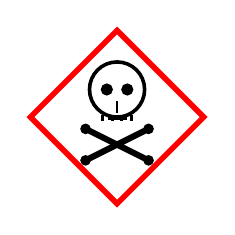
\begin{tikzpicture}
                \draw[draw=red, line width=2pt, fill=white] (0,-1.1) -- (1.1,0) -- (0,1.1) -- (-1.1,0) -- cycle;
                \draw[line width=1.3pt] (0,0.35) circle (0.35);
                \filldraw[black] (-0.13,0.35) circle (0.07);
                \filldraw[black] (0.13,0.35) circle (0.07);
                \draw[line width=1pt] (0,0.2) -- (0,0.05);
                \draw[line width=1pt] (-0.12,-0.02) -- (0.12,-0.02);
                \draw[line width=1pt] (-0.18,-0.05) -- (-0.18,0.02);
                \draw[line width=1pt] (-0.06,-0.05) -- (-0.06,0.02);
                \draw[line width=1pt] (0.06,-0.05) -- (0.06,0.02);
                \draw[line width=1pt] (0.18,-0.05) -- (0.18,0.02);
                \draw[line width=2.2pt] (-0.4,-0.55) -- (0.4,-0.15);
                \draw[line width=2.2pt] (-0.4,-0.15) -- (0.4,-0.55);
                \filldraw[black] (-0.4,-0.55) circle (0.06);
                \filldraw[black] (0.4,-0.15) circle (0.06);
                \filldraw[black] (-0.4,-0.15) circle (0.06);
                \filldraw[black] (0.4,-0.55) circle (0.06);
            \end{tikzpicture}\\[2pt]
            \textbf{Toxic}\\[2pt]
            {\small Can kill or seriously harm you, even in small amounts. Example: some pesticides.}
        \end{minipage}
        \\[9mm]
        \begin{minipage}{5.0cm}
            \centering
            
\begin{tikzpicture}
                \draw[draw=red, line width=2pt, fill=white] (0,-1.1) -- (1.1,0) -- (0,1.1) -- (-1.1,0) -- cycle;
                \draw[line width=5pt, line cap=round] (0,-0.05) -- (0,0.65);
                \filldraw[black] (0,-0.45) circle (0.1);
            \end{tikzpicture}\\[2pt]
            \textbf{Harmful / Irritant}\\[2pt]
            {\small Irritates skin or eyes, or is harmful if swallowed. Example: some detergents.}
        \end{minipage}
        &
        \begin{minipage}{5.0cm}
            \centering
            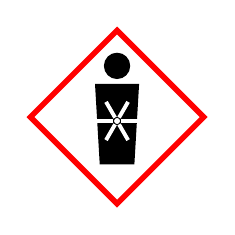
\begin{tikzpicture}
                \draw[draw=red, line width=2pt, fill=white] (0,-1.1) -- (1.1,0) -- (0,1.1) -- (-1.1,0) -- cycle;
                \filldraw[black] (0,0.65) circle (0.16);
                \fill[black] (-0.28,0.42) -- (0.28,0.42) -- (0.22,-0.6) -- (-0.22,-0.6) -- cycle;
                \begin{scope}[shift={(0,-0.05)}]
                    \foreach \a in {0,60,120,180,240,300}{
                        \draw[white, line width=1.4pt] (\a:0.05) -- (\a:0.28);
                    }
                \end{scope}
                \filldraw[white] (0,-0.05) circle (0.03);
            \end{tikzpicture}\\[2pt]
            \textbf{Health hazard}\\[2pt]
            {\small Can cause serious long-term damage (e.g.\ to the lungs). Example: tobacco smoke, asbestos.}
        \end{minipage}
        &
        \begin{minipage}{5.0cm}
            \centering
            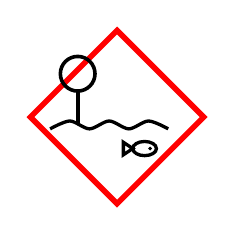
\begin{tikzpicture}
                \draw[draw=red, line width=2pt, fill=white] (0,-1.1) -- (1.1,0) -- (0,1.1) -- (-1.1,0) -- cycle;
                \draw[line width=1.4pt] (-0.5,-0.1) -- (-0.5,0.35);
                \draw[line width=1.3pt] (-0.5,0.55) circle (0.22);
                \draw[line width=1.2pt] plot[smooth] coordinates {(-0.85,-0.15) (-0.6,-0.05) (-0.35,-0.15) (-0.1,-0.05) (0.15,-0.15) (0.4,-0.05) (0.65,-0.15)};
                \draw[line width=1.2pt] (0.35,-0.4) ellipse (0.15 and 0.09);
                \draw[line width=1.2pt] (0.2,-0.4) -- (0.08,-0.32) -- (0.08,-0.48) -- cycle;
                \filldraw[black] (0.42,-0.4) circle (0.015);
            \end{tikzpicture}\\[2pt]
            \textbf{Environmental hazard}\\[2pt]
            {\small Poisonous to plants, fish or other wildlife. Example: some pesticides and solvents.}
        \end{minipage}
    \end{tabular}
    \caption{The nine GHS hazard pictograms: a black symbol on a white background, inside a red diamond.}
\end{figure}

\begin{impt}
    A single product can carry more than one pictogram at the same time (for example, a drain cleaner can be both corrosive and toxic). Always read \textbf{all} the pictograms on a label before using a product.
\end{impt}

\begin{exercise}
    A bottle of concentrated hydrochloric acid shows the \negsubro{corrosive} pictogram, and a bottle of ethanol shows the \negsubro{flammable} pictogram. Explain, in your own words, what danger each pictogram warns about, and say one safety measure you should take with each product.
    \begin{solu}
        The \textbf{corrosive} pictogram warns that the acid can burn the skin and eyes and damage materials on contact, so we should wear gloves and goggles and avoid any contact with skin. \\
        The \textbf{flammable} pictogram warns that ethanol catches fire easily, so we should keep it away from flames and heat sources, such as a lit Bunsen burner.
    \end{solu}
\end{exercise}

\begin{exercise}
    A student is going to heat a test tube containing a liquid with a Bunsen burner and then measure its volume once it has cooled down.
    \begin{enumerate}[label=\letraminuscula]
        \item List the equipment and safety items this student should use for the whole activity.
        \item Explain why the test tube must be pointed away from people while it is being heated.
    \end{enumerate}
    \begin{solu}
        \begin{enumerate}[label=\alph*)]
            \item Safety goggles, lab coat, tongs or a test-tube holder to handle the hot test tube, a Bunsen burner, a test tube, and a graduated cylinder to measure the volume of the liquid once it has cooled.
            \item Heated liquids can splash or the tube's contents can be suddenly expelled (bumping); pointing it away from people prevents anyone from being burnt if this happens.
        \end{enumerate}
    \end{solu}
\end{exercise}

\begin{exercise}
    In a laboratory session, a student eats a sandwich while waiting for an experiment to finish, does not tie back her long hair before lighting the Bunsen burner, and pours the leftover chemical down the sink at the end of the class.
    \begin{enumerate}[label=\letraminuscula]
        \item Identify the three safety violations described.
        \item For each one, explain briefly what should have been done instead.
    \end{enumerate}
    \begin{solu}
        \begin{enumerate}[label=\alph*)]
            \item Eating in the laboratory; working with a flame with loose long hair; disposing of chemical waste down the sink.
            \item Food and drink must never be brought into the laboratory; long hair must always be tied back before using a flame, to avoid it catching fire; chemical waste must be poured into the correct labelled waste container, never down the sink.
        \end{enumerate}
    \end{solu}
\end{exercise}

%----------------------------------------------------------------------------------------

\section*{Summary}

\begin{itemize}
    \item \textbf{Scientific method}: observation, hypothesis, experimentation, analysis of results and conclusions; scientists communicate results using scientific language, based on the SI.
    \item \textbf{Matter}: everything that has mass and occupies space. It forms \textbf{bodies} (defined boundaries) or \textbf{material systems} (no defined boundaries).
    \item \textbf{Properties}: quantitative/qualitative, extensive/intensive, general/characteristic (density, melting and boiling points, solubility, conductivity, hardness).
    \item \textbf{Density and floating}: a substance floats in a liquid if its density is lower than the liquid's, and sinks if it is higher.
    \item \textbf{Isolating a quantity}: do the same operation on both sides of the equation: \(d = m/V\), \(m = d \cdot V\), \(V = m/d\).
    \item \textbf{Quantity, unit, measure}: a quantity is measured by comparing it with a unit; the SI fixes the units, multiples and submultiples for each quantity.
    \item \textbf{Fundamental and derived quantities}: the SI has seven fundamental quantities (length, mass, time, temperature, amount of substance, electric current and luminous intensity); all the others (surface area, volume, density, speed, pressure, energy\ldots) are derived from them.
    \item \textbf{Multiples and submultiples}: prefixes (giga, mega, kilo, hecto, deca, deci, centi, milli, micro, nano) worth a power of 10, used to write measurements with simple numbers.
    \item \textbf{Conversion factor}: a fraction of equal amounts in different units, worth 1, used to change the unit of a quantity without changing its value. The 1 always goes with the bigger unit, and we use powers of 10.
    \item \textbf{Length, mass \& capacity}: steps of \(10\); \textbf{surface area}: square the factor of length (steps of \(10^{2}\)); \textbf{volume}: cube the factor of length (steps of \(10^{3}\)).
    \item \textbf{Volume--capacity}: \(\qty{1}{\cubic\metre} = \qty{1}{\kilo\litre}\); \(\qty{1}{\cubic\dm} = \qty{1}{\litre}\); \(\qty{1}{\cubic\cm} = \qty{1}{\mL}\).
    \item \textbf{Time}: \(\qty{1}{\minute} = \qty{60}{\s}\), \(\qty{1}{\hour} = \qty{3600}{\s}\), \(\qty{1}{\day} = \qty{24}{\hour}\), 1 week = 7 days, 1 year = 365 days. \textbf{Speed} and \textbf{density} need two conversion factors.
    \item \textbf{Scientific notation}: \(a \cdot 10^{n}\), with one non-zero digit before the comma. Big numbers \(\to\) the comma jumps left, positive exponent; small numbers \(\to\) the comma jumps right, negative exponent.
    \item \textbf{Pressure and energy}: \(\qty{1}{\atmospher} = \qty{760}{\mmhg} = \qty{101325}{\Pa}\); \(\qty{1}{\calorie} = \qty{4.18}{\J}\).
    \item \textbf{Instruments}: scales for mass; graduated cylinders, burettes and pipettes for volume (reading at the bottom of the meniscus).
    \item \textbf{Sensitivity, precision and accuracy}: the sensitivity of an instrument is its smallest division; a precise measurement gives many stable decimal places, while an accurate one is close to the real value.
    \item \textbf{Indirect measurement}: a quantity calculated from other, directly measured, quantities (surface area, density, small thicknesses\ldots).
    \item \textbf{Laboratory equipment}: test tubes, beakers, Erlenmeyer flasks, graduated cylinders and Bunsen burners, used together with safety goggles, a lab coat and a fume hood.
    \item \textbf{Safety rules}: always wear protective equipment, never eat or work alone, know where the eyewash station and fire extinguisher are, and dispose of waste correctly.
    \item \textbf{Hazard pictograms (GHS)}: nine standardised symbols, black on white inside a red diamond, that warn about the dangers of a chemical product (explosive, flammable, oxidizing, compressed gas, corrosive, toxic, harmful/irritant, health hazard, environmental hazard).
\end{itemize}

\section{Vocabulary}

\begin{vocabulary}[Scientific method]
    An organised set of steps (observation, hypothesis, experimentation, analysis and conclusions) used to answer questions about nature. \newline
    \textbf{Translation to Spanish}: Método científico
\end{vocabulary}

\begin{vocabulary}[Hypothesis]
    A possible, testable explanation for an observed fact. \newline
    \textbf{Translation to Spanish}: Hipótesis
\end{vocabulary}

\begin{vocabulary}[Matter]
    Everything that occupies space and has mass. \newline
    \textbf{Translation to Spanish}: Materia
\end{vocabulary}

\begin{vocabulary}[Body]
    Matter with defined boundaries. \newline
    \textbf{Translation to Spanish}: Cuerpo
\end{vocabulary}

\begin{vocabulary}[Material system]
    Matter with no defined boundaries. \newline
    \textbf{Translation to Spanish}: Sistema material
\end{vocabulary}

\begin{vocabulary}[Property]
    An aspect of matter that can be evaluated. \newline
    \textbf{Translation to Spanish}: Propiedad
\end{vocabulary}

\begin{vocabulary}[Quantity]
    A property of matter that can be measured. \newline
    \textbf{Translation to Spanish}: Magnitud
\end{vocabulary}

\begin{vocabulary}[Fundamental quantity]
    A quantity defined by itself, without using other quantities (length, mass, time\ldots). \newline
    \textbf{Translation to Spanish}: Magnitud fundamental
\end{vocabulary}

\begin{vocabulary}[Derived quantity]
    A quantity obtained by combining fundamental quantities (surface area, volume, speed\ldots). \newline
    \textbf{Translation to Spanish}: Magnitud derivada
\end{vocabulary}

\begin{vocabulary}[Prefix]
    A word or symbol placed before a unit to form a multiple or a submultiple of it (kilo-, centi-\ldots). \newline
    \textbf{Translation to Spanish}: Prefijo
\end{vocabulary}

\begin{vocabulary}[Multiple / Submultiple]
    A unit bigger / smaller than the base unit by a power of 10. \newline
    \textbf{Translation to Spanish}: Múltiplo / Submúltiplo
\end{vocabulary}

\begin{vocabulary}[Unit]
    A known amount of a quantity used as a reference for measuring. \newline
    \textbf{Translation to Spanish}: Unidad
\end{vocabulary}

\begin{vocabulary}[Density]
    Mass per unit of volume. \newline
    \textbf{Translation to Spanish}: Densidad
\end{vocabulary}

\begin{vocabulary}[Solubility]
    Maximum amount of a solute that can dissolve in \qty{100}{\g} of solvent. \newline
    \textbf{Translation to Spanish}: Solubilidad
\end{vocabulary}

\begin{vocabulary}[Floating]
    Situation in which a substance placed in a liquid stays on the surface because its density is lower than that of the liquid. \newline
    \textbf{Translation to Spanish}: Flotar / Flotación
\end{vocabulary}

\begin{vocabulary}[Sensitivity]
    The smallest amount that an instrument can measure. \newline
    \textbf{Translation to Spanish}: Sensibilidad (apreciación)
\end{vocabulary}

\begin{vocabulary}[Precision]
    How many stable decimal places, or how small a variation, an instrument or measurement can distinguish. \newline
    \textbf{Translation to Spanish}: Precisión
\end{vocabulary}

\begin{vocabulary}[Accuracy]
    How close a measurement is to the real value of the quantity. \newline
    \textbf{Translation to Spanish}: Exactitud
\end{vocabulary}

\begin{vocabulary}[Meniscus]
    Curve formed by the surface of a liquid inside a narrow tube. \newline
    \textbf{Translation to Spanish}: Menisco
\end{vocabulary}

\begin{vocabulary}[Indirect measurement]
    A measurement obtained through calculations from other, direct, measurements. \newline
    \textbf{Translation to Spanish}: Medida indirecta
\end{vocabulary}

\begin{vocabulary}[Conversion factor]
    A fraction of equal amounts expressed in different units, used to change units. \newline
    \textbf{Translation to Spanish}: Factor de conversión
\end{vocabulary}

\begin{vocabulary}[Scientific notation]
    A way of writing a number as a coefficient (from 1 to 9,99\ldots) multiplied by a power of 10. \newline
    \textbf{Translation to Spanish}: Notación científica
\end{vocabulary}

\begin{vocabulary}[Exponent]
    The small number written at the top right of a power; it tells us how many times we multiply (or divide) by 10. \newline
    \textbf{Translation to Spanish}: Exponente
\end{vocabulary}

\begin{vocabulary}[To isolate (a quantity)]
    To leave a quantity alone on one side of an equation, doing the same operation on both sides. \newline
    \textbf{Translation to Spanish}: Despejar (una magnitud)
\end{vocabulary}

\begin{vocabulary}[Hazard pictogram]
    A standardised symbol on a chemical product's label that warns about the type of danger it presents. \newline
    \textbf{Translation to Spanish}: Pictograma de peligrosidad
\end{vocabulary}

\begin{vocabulary}[Corrosive]
    Able to burn the skin and eyes and destroy materials on contact. \newline
    \textbf{Translation to Spanish}: Corrosivo
\end{vocabulary}

\begin{vocabulary}[Flammable]
    Able to catch fire easily. \newline
    \textbf{Translation to Spanish}: Inflamable
\end{vocabulary}

\begin{vocabulary}[Fume hood]
    A ventilated cabinet that extracts dangerous gases or vapours from the laboratory. \newline
    \textbf{Translation to Spanish}: Vitrina de gases / Campana extractora
\end{vocabulary}

\begin{vocabulary}[Safety goggles]
    Glasses that protect the eyes from splashes, dust and vapours. \newline
    \textbf{Translation to Spanish}: Gafas de seguridad
\end{vocabulary}

\begin{vocabulary}[Bunsen burner]
    A gas burner used as a heat source in the laboratory. \newline
    \textbf{Translation to Spanish}: Mechero Bunsen
\end{vocabulary}



%------------------------------------------------


    \chapterimage{images/portada_cabeceras/cabecera_Unit2}
    \chapter{States of Matter}
    % Saberes básicos (LOMLOE) asociados a esta unidad
%
% B. La materia
%   - Teoría cinético-molecular: aplicación a observaciones sobre la materia explicando
%     sus propiedades, los estados de agregación y los cambios de estado. Es el eje
%     central de la unidad: toda la unidad explica los estados de agregación (sólido,
%     líquido, gas) y los cambios de estado (fusión, ebullición, evaporación,
%     sublimación...) a partir del modelo de partículas en movimiento.
%   - Experimentos relacionados con los sistemas materiales: conocimiento y descripción
%     de sus propiedades. Se describen propiedades como la compresibilidad, la
%     densidad relativa de los estados o la presión de un gas, ligadas al
%     comportamiento de las partículas.
%
% C. La energía
%   - Efectos del calor sobre la materia: análisis de los efectos y aplicación en
%     situaciones cotidianas. Se estudia cómo el calor produce cambios de estado, la
%     curva de calentamiento/enfriamiento y el concepto de calor latente, así como
%     fenómenos cotidianos (niebla, rocío, olla a presión, altitud y ebullición...).
%
% A. Las destrezas científicas básicas
%   - El lenguaje científico: unidades del Sistema Internacional. Se usan
%     sistemáticamente unidades de presión, volumen y temperatura (atmósferas, litros,
%     kelvin) y el manejo de \qty{}{} de siunitx en los ejemplos y ejercicios numéricos
%     de las leyes de los gases.
%   - Estrategias de interpretación y producción de información científica. Se
%     interpretan tablas de puntos de fusión/ebullición y gráficas de calentamiento
%     descritas verbalmente para extraer conclusiones.

\spacing{1.3}
\raggedbottom % pages with large figures end where the text ends (no stretched gaps between boxes)

\section{Physical states of matter}

On the Earth, almost everything around us is a \textbf{solid}, a \textbf{liquid} or a \textbf{gas}. Each state has its own ``personality'':

\begin{figure}[H]
    \centering
    % [FIGURA ORIGINAL] \includegraphics[width=\textwidth]{Unit_2/states_overview}
    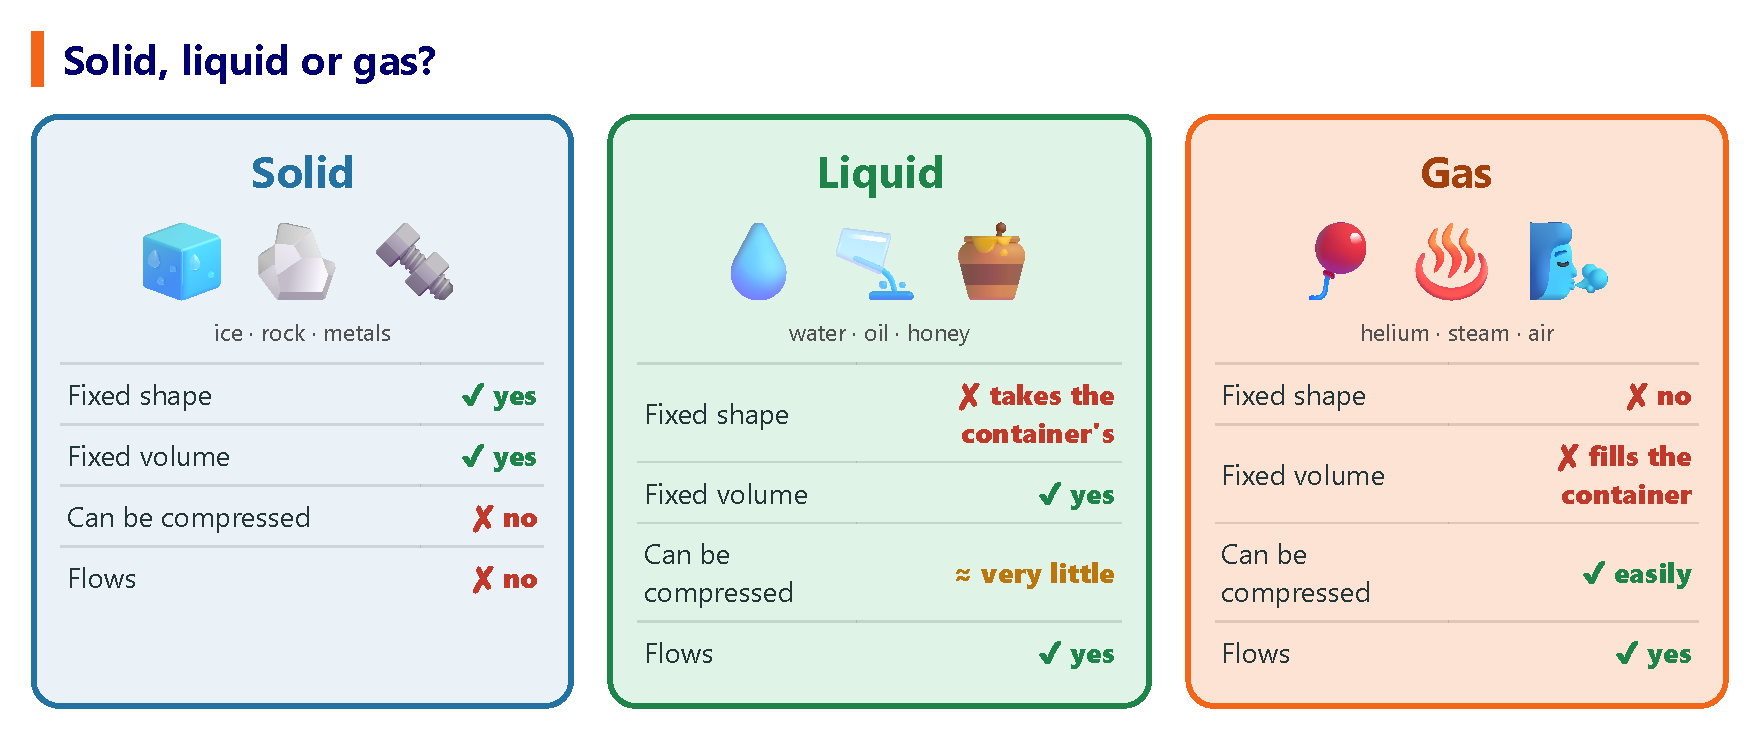
\includegraphics[width=\textwidth]{FigurasSVG/Unit_2_State_of_Matter/pdf/states_overview.pdf}
    \caption{The properties of solids, liquids and gases.}
    \label{fig:u2_states_overview}
\end{figure}

\subsection{Plasma: the fourth state of matter}

Solid, liquid and gas are not the only states of matter. There is a \negsubro{fourth state}, called \textbf{plasma}.

\begin{definition}[Plasma]
    A gas that is so \textbf{hot} that its particles break and become \textbf{electrically charged}. That is why a plasma \textbf{glows} (gives out light) and conducts electricity. It is considered the \textbf{fourth state of matter}.
\end{definition}

\begin{figure}[H]
    \centering
    % [FIGURA ORIGINAL] \includegraphics[width=\textwidth]{Unit_2/plasma}
    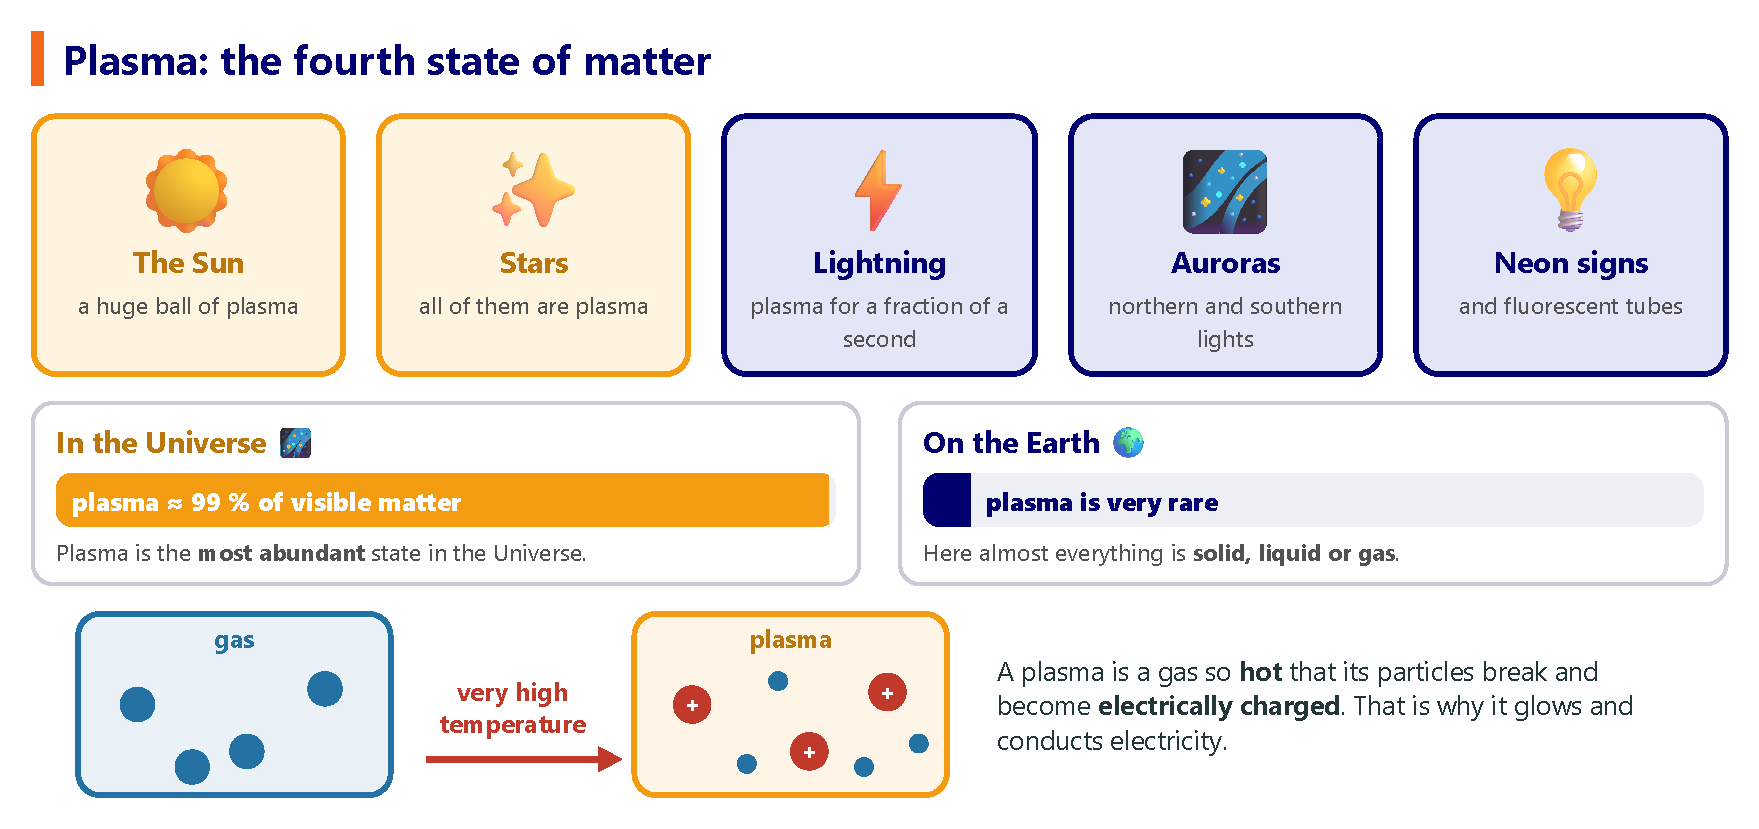
\includegraphics[width=\textwidth]{FigurasSVG/Unit_2_State_of_Matter/pdf/plasma.pdf}
    \caption{Plasma is the most abundant state in the Universe, but it is very rare on the Earth.}
    \label{fig:u2_plasma}
\end{figure}

\begin{impt}
    \begin{itemize}
        \item Plasma is the \textbf{most abundant} state of matter \textbf{in the Universe}: the \textbf{Sun} and all the stars are huge balls of plasma.
        \item On the \textbf{Earth}, however, plasma is \textbf{very rare}: we only see it in lightning, in the auroras (northern lights) and in neon signs and fluorescent tubes.
    \end{itemize}
\end{impt}

\begin{didyouknow}
    There are also \textbf{liquid crystals}, a strange state between a liquid and a solid. They are used in the LCD screens of mobile phones and televisions.
\end{didyouknow}

\begin{exercise}
    Classify each substance as a solid, a liquid or a gas at room temperature: wood, natural gas, oil, water, aluminium, oxygen, alcohol, carbon dioxide, sand.
    \begin{solu}
        \textbf{Solids}: wood, aluminium, sand. \\
        \textbf{Liquids}: oil, water, alcohol. \\
        \textbf{Gases}: natural gas, oxygen, carbon dioxide.
    \end{solu}
\end{exercise}

\begin{exercise}
    Answer these questions about plasma:
    \begin{enumerate}[label=\letraminuscula]
        \item Why is plasma called the ``fourth state of matter''?
        \item Which is the most abundant state of matter in the Universe? And on the Earth?
        \item Give two examples of plasma that you can see on the Earth.
    \end{enumerate}
    \begin{solu}
        \begin{enumerate}[label=\alph*)]
            \item Because it is different from solids, liquids and gases: it is a gas so hot that its particles are electrically charged.
            \item In the Universe, plasma (the Sun and the stars). On the Earth, plasma is very rare: most matter is solid, liquid or gas.
            \item Lightning, auroras, neon signs, fluorescent tubes.
        \end{enumerate}
    \end{solu}
\end{exercise}

\begin{exercise}
    Decide whether each statement is true or false, and correct the false ones.
    \begin{enumerate}[label=\letraminuscula]
        \item Sand flows, so it is a liquid.
        \item A sponge can be compressed, so it is a gas.
        \item The sponge is made of a porous, flexible material with air inside, so it can be compressed.
    \end{enumerate}
    \begin{solu}
        \begin{enumerate}[label=\alph*)]
            \item \textbf{False}. Sand is a solid made up of very small grains that seem to behave like a liquid, but each grain keeps its own shape and size.
            \item \textbf{False}. A sponge is a solid; it is compressible because it is porous (it has air inside), not because it is a gas.
            \item \textbf{True}.
        \end{enumerate}
    \end{solu}
\end{exercise}

\begin{exercise}
    A student has three identical closed syringes: syringe A contains air, syringe B contains water, and syringe C contains a small metal ball. The student blocks the tip of each syringe and pushes the plunger as hard as possible.
    \begin{enumerate}[label=\letraminuscula]
        \item In which syringe can the plunger be pushed in noticeably?
        \item Explain the result in terms of the compressibility of solids, liquids and gases.
    \end{enumerate}
    \begin{solu}
        \begin{enumerate}[label=\alph*)]
            \item Only in \textbf{syringe A} (the one with air).
            \item Gases can be compressed because there is a lot of empty space between their particles. Liquids (syringe B) and solids (syringe C) cannot be compressed, since their particles are already almost touching.
        \end{enumerate}
    \end{solu}
\end{exercise}

%----------------------------------------------------------------------------------------

\section{Kinetic theory and states of matter}

Why is ice hard, water runny and steam invisible, if all three are the same substance? To answer this question, scientists imagine matter as if it were made of tiny ``balls''. This idea is called the \negsubro{kinetic theory} (``kinetic'' comes from a Greek word that means ``movement'').

\begin{definition}[Kinetic theory]
    A scientific model that explains how matter behaves by imagining that it is made of tiny \textbf{particles} that are \textbf{always moving}.
\end{definition}

The kinetic theory can be summed up in four simple ideas:

\begin{enumerate}[label=\numberballmDarkTeal]
    \item \textbf{Everything is made of particles.} All matter is made of tiny particles, so small that we cannot see them, not even with a normal microscope.
    \item \textbf{The particles never stop moving.} They vibrate, move around and bump into each other all the time.
    \item \textbf{Hotter means faster.} When we heat a substance, its particles move faster; when we cool it, they move more slowly. \textbf{Temperature} tells us how fast the particles are moving.
    \item \textbf{The particles attract each other.} They are held together by forces, like invisible ``glue''. How strong this glue is, compared with how fast the particles move, decides whether the substance is a \textbf{solid}, a \textbf{liquid} or a \textbf{gas}.
\end{enumerate}

\begin{impt}
    Think of the pupils in your school: in class they are sitting in their places and only fidget a little (\textbf{solid}); in the corridor they walk and move past each other, but stay close together (\textbf{liquid}); in the playground they run freely in all directions, far from each other (\textbf{gas}).
\end{impt}

\begin{figure}[H]
    \centering
    % [FIGURA ORIGINAL] \includegraphics[width=\textwidth]{Unit_2/particle_model}
    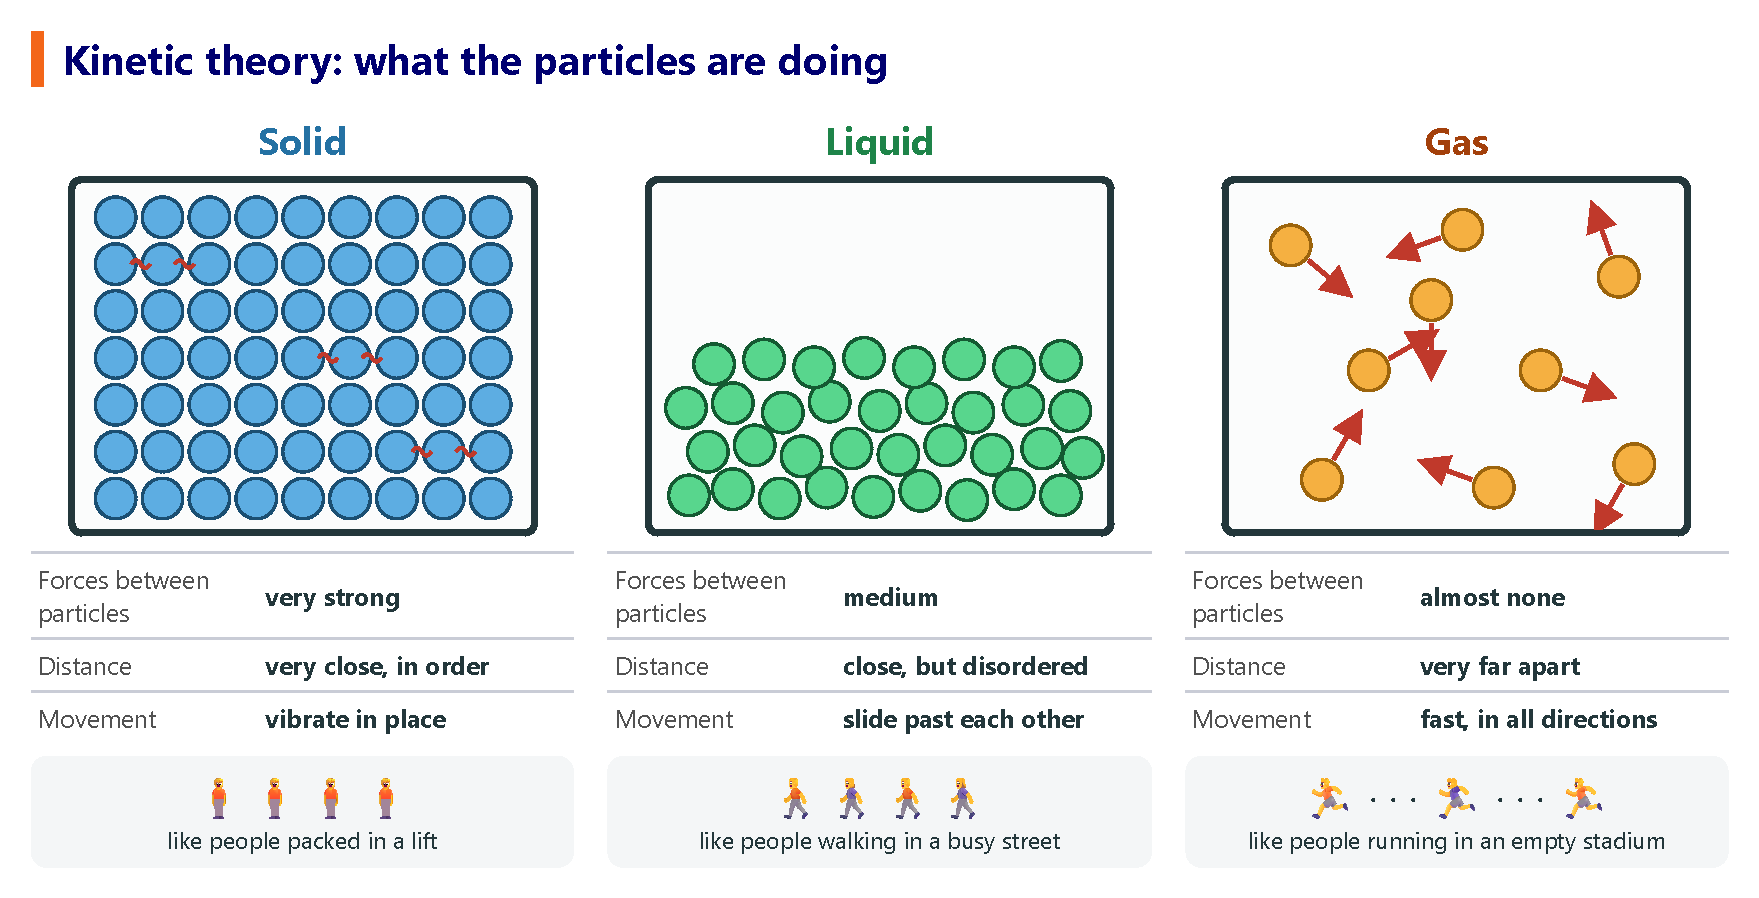
\includegraphics[width=\textwidth]{FigurasSVG/Unit_2_State_of_Matter/pdf/particle_model.pdf}
    \caption{The particle model of the three states of matter.}
    \label{fig:u2_particle_model}
\end{figure}

\begin{impt}
    Because their particles are so close together, solids usually have the \textbf{highest} density, liquids a little lower, and gases a \textbf{very low} density.
\end{impt}

\subsection{Gas pressure}

\begin{definition}[Pressure of a gas]
    The result of the particles of a gas \textbf{hitting the walls} of their container. More hits, or stronger hits, mean more pressure.
\end{definition}

\begin{figure}[H]
    \centering
    % [FIGURA ORIGINAL] \includegraphics[width=\textwidth]{Unit_2/gas_pressure}
    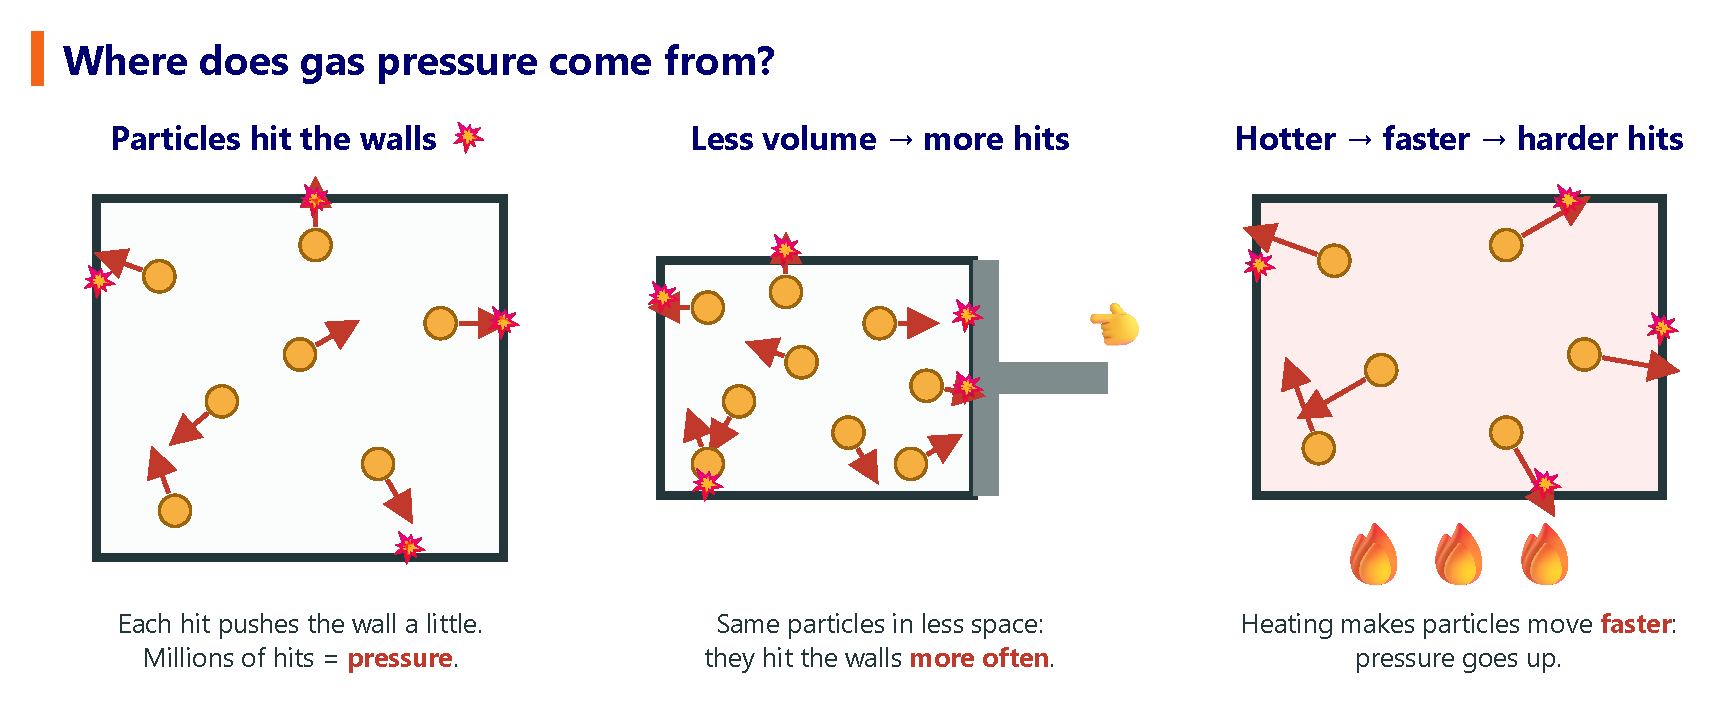
\includegraphics[width=\textwidth]{FigurasSVG/Unit_2_State_of_Matter/pdf/gas_pressure.pdf}
    \caption{Gas pressure increases if the volume decreases or the temperature increases.}
    \label{fig:u2_gas_pressure}
\end{figure}

\begin{exercise}
    Use kinetic theory to explain why a block of metal expands slightly when it is heated, but does not change its state of matter.
    \begin{solu}
        Heating makes the particles of the solid vibrate more, so the distance between them increases slightly; but the forces between the particles are still strong enough to keep the rigid structure, so the substance is still a solid, only a little larger.
    \end{solu}
\end{exercise}

\begin{exercise}
    An iceberg floats in the sea.
    \begin{enumerate}[label=\letraminuscula]
        \item Use kinetic theory to explain whether the particles are further apart in ice or in liquid water.
        \item What will happen to sea level if the iceberg melts?
    \end{enumerate}
    \begin{solu}
        \begin{enumerate}[label=\alph*)]
            \item Since ice floats, it is \textbf{less dense} than liquid water; therefore its particles are \textbf{further apart} in the solid than in the liquid (water is an unusual substance in this respect).
            \item The iceberg is already floating, so it already displaces a volume of water equal to its own weight; when it melts, sea level does \textbf{not} rise (unlike ice melting on land, which adds extra water to the sea).
        \end{enumerate}
    \end{solu}
\end{exercise}

\begin{exercise}
    The density of some gases at room temperature is: oxygen \qty{1.33}{\kg\per\cubic\metre}, helium \qty{0.17}{\kg\per\cubic\metre}, air \qty{1.20}{\kg\per\cubic\metre}. Explain why helium balloons float in air, while oxygen balloons would not.
    \begin{solu}
        A balloon floats in air when it is \textbf{less dense} than air. Helium (\qty{0.17}{\kg\per\cubic\metre}) is much less dense than air (\qty{1.20}{\kg\per\cubic\metre}), so it floats. Oxygen (\qty{1.33}{\kg\per\cubic\metre}) is denser than air, so an oxygen balloon would sink.
    \end{solu}
\end{exercise}

\begin{exercise}
    Two identical closed balloons are filled with the same amount of air. One is left in a fridge and the other next to a radiator. Use kinetic theory to predict which balloon will end up larger.
    \begin{solu}
        The balloon next to the \textbf{radiator}. Heat makes the air particles inside it move faster, so they hit the walls harder and more often; the pressure increases and pushes the walls outwards. In the cold balloon the particles move more slowly, the pressure is lower and the balloon stays smaller.
    \end{solu}
\end{exercise}

\subsection{Kinetic theory explains everyday phenomena}

\begin{figure}[H]
    \centering
    % [FIGURA ORIGINAL] \includegraphics[width=\textwidth]{Unit_2/everyday_kinetic}
    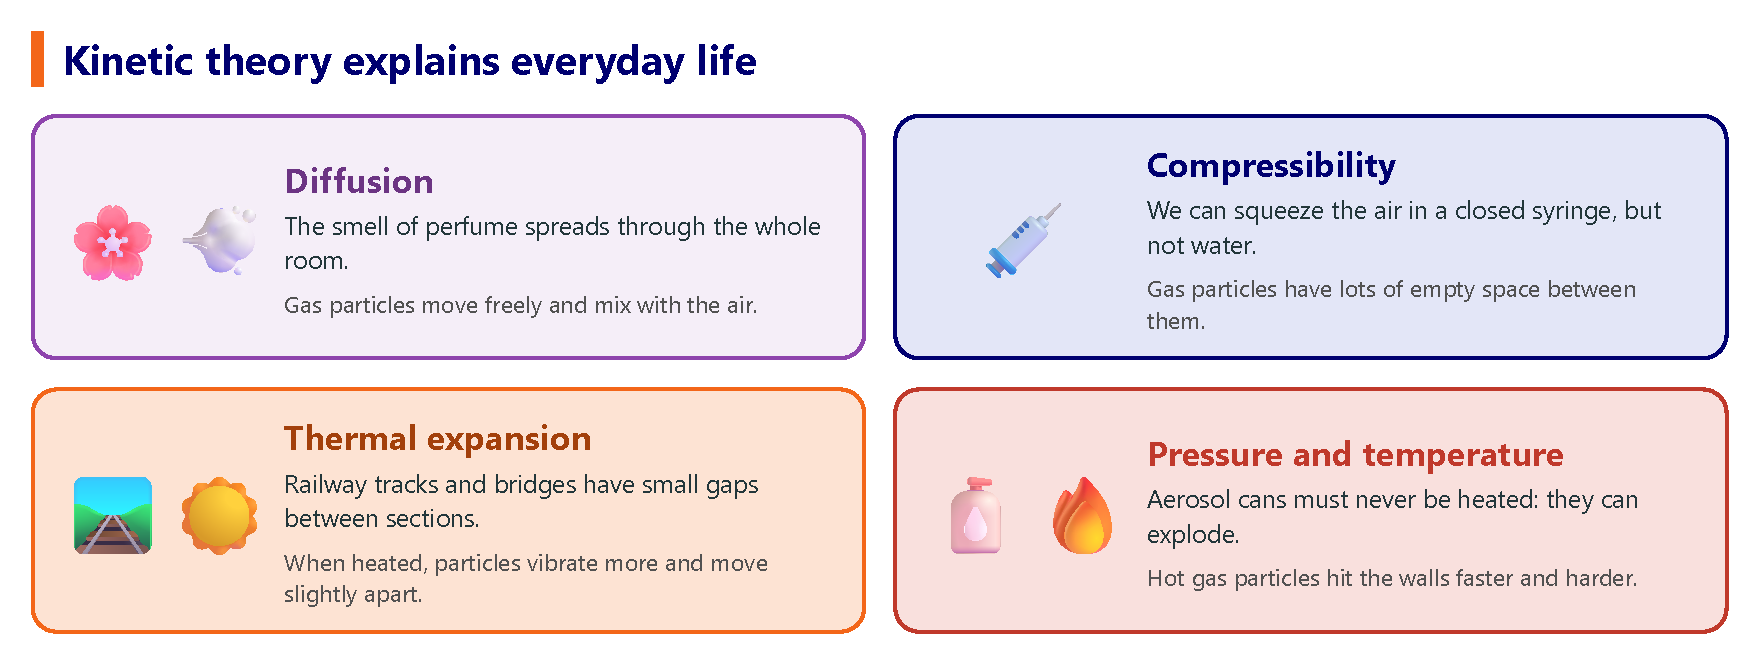
\includegraphics[width=\textwidth]{FigurasSVG/Unit_2_State_of_Matter/pdf/everyday_kinetic.pdf}
    \caption{Four everyday phenomena explained with particles.}
    \label{fig:u2_everyday_kinetic}
\end{figure}

\begin{definition}[Diffusion]
    The spreading of the particles of a substance until they mix completely with the particles of another one. It happens quickly in gases and more slowly in liquids (a drop of ink in water).
\end{definition}

\begin{exercise}
    Use kinetic theory (diffusion, expansion, compressibility) to explain each situation.
    \begin{enumerate}[label=\letraminuscula]
        \item You can smell food cooking in the kitchen from another room.
        \item A metal lid on a glass jar becomes easier to unscrew after running hot water over it.
        \item A bicycle pump becomes harder to push as you compress the air inside it.
    \end{enumerate}
    \begin{solu}
        \begin{enumerate}[label=\alph*)]
            \item The particles released by the food spread out by \textbf{diffusion} through the air until they reach your nose.
            \item Heat makes the metal particles in the lid vibrate more and move slightly apart, so the lid \textbf{expands} more than the glass and becomes looser.
            \item The same number of gas particles are squeezed into a smaller volume; they hit the piston more often, so the \textbf{pressure} (and the force needed to push) increases.
        \end{enumerate}
    \end{solu}
\end{exercise}

\begin{exercise}
    Perfume spreads across a room faster on a hot day than on a cold day. Use kinetic theory to explain why.
    \begin{solu}
        On a hot day the particles move \textbf{faster}, on average, than on a cold day. Diffusion is caused by the random motion of particles, so faster particles spread out and mix with the air more quickly.
    \end{solu}
\end{exercise}

\begin{exercise}
    A sealed bag of crisps looks normal at sea level, but when a plane climbs to cruising altitude, the same bag looks swollen.
    \begin{enumerate}[label=\letraminuscula]
        \item What happens to the air pressure outside the bag as the plane climbs?
        \item Use kinetic theory to explain why the bag swells up.
    \end{enumerate}
    \begin{solu}
        \begin{enumerate}[label=\alph*)]
            \item The air pressure \textbf{outside} the bag decreases as altitude increases.
            \item The air inside the bag keeps hitting the inner walls with the same force as before, while the air outside pushes back with less force. The outward push is greater, so the bag expands until the pressures balance (or it may even burst).
        \end{enumerate}
    \end{solu}
\end{exercise}

%----------------------------------------------------------------------------------------

\section{Gas laws}

The behaviour of a gas depends on three quantities: \textbf{pressure} \(p\), \textbf{volume} \(V\) and \textbf{temperature} \(T\). Each gas law keeps \textbf{one} of them constant and tells us how the other two are related.

\subsection{The Kelvin scale}

\begin{figure}[H]
    \centering
    % [FIGURA ORIGINAL] \includegraphics[width=0.95\textwidth]{Unit_2/kelvin_scale}
    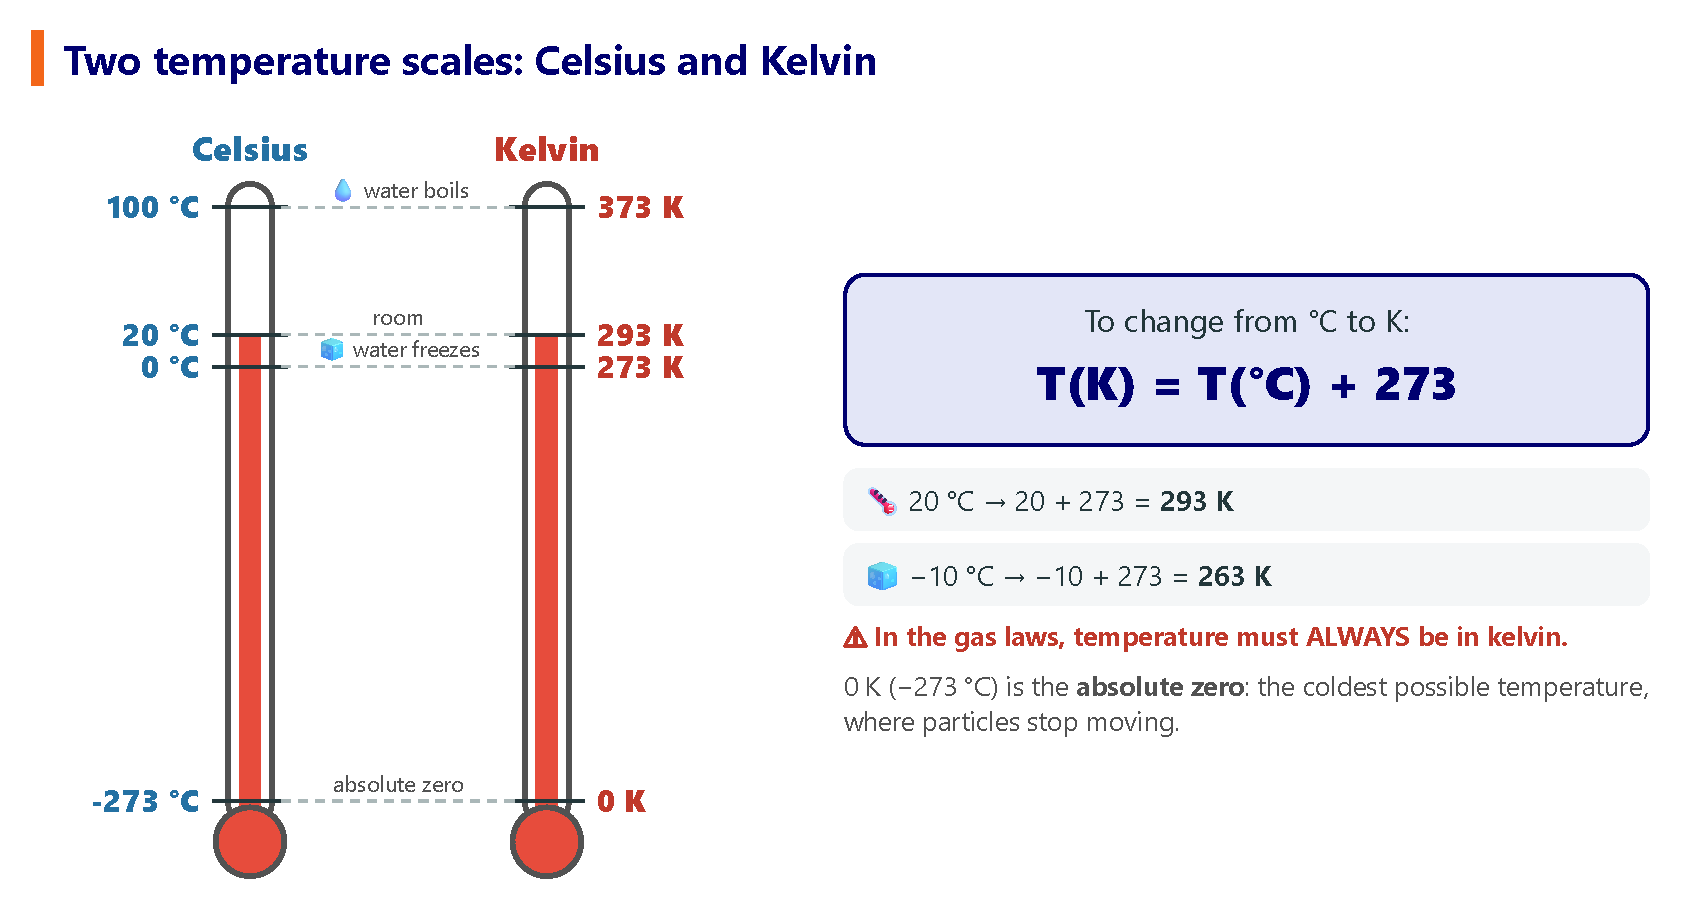
\includegraphics[width=0.95\textwidth]{FigurasSVG/Unit_2_State_of_Matter/pdf/kelvin_scale.pdf}
    \caption{The Celsius and Kelvin scales: same size of degree, different zero.}
    \label{fig:u2_kelvin_scale}
\end{figure}

\begin{impt}
    In \textbf{all} the gas laws, temperature must be in \textbf{kelvin}:
    \begin{equation*}
        T(\unit{\K}) = T(\unit{\celsius}) + 273
    \end{equation*}
\end{impt}

\subsection{What do the numbers 1 and 2 mean?}

In all the gas laws you will see the quantities written with a small number: \(p_1\), \(V_1\), \(T_1\) and \(p_2\), \(V_2\), \(T_2\). These small numbers are called \textbf{subscripts}, and they are very important:

\begin{impt}
    In the gas laws we always study the \textbf{same gas} at two different moments:
    \begin{itemize}
        \item The subscript \textbf{1} means the \textbf{beginning} (the \textbf{initial} state): how the gas is \textbf{before} the change.
        \item The subscript \textbf{2} means the \textbf{end} (the \textbf{final} state): how the gas is \textbf{after} something has changed (we heat it, cool it, compress it or let it expand).
    \end{itemize}
    For example, \(V_1\) is the volume \textbf{before} the change and \(V_2\) is the volume \textbf{after} the change.
\end{impt}

\begin{figure}[H]
    \centering
    % [FIGURA ORIGINAL] \includegraphics[width=\textwidth]{Unit_2/states_1_2}
    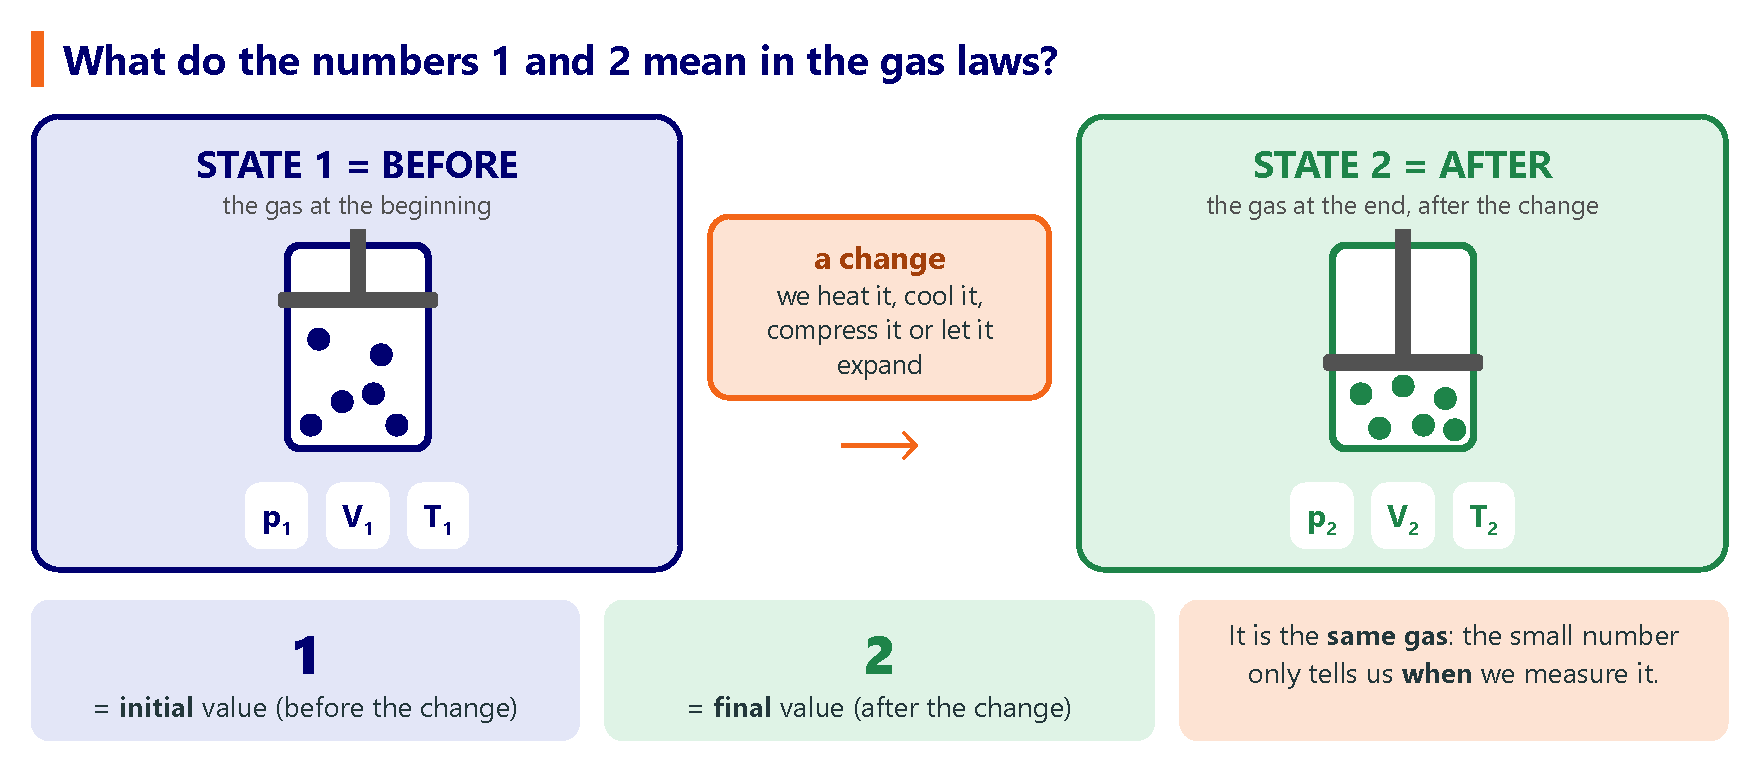
\includegraphics[width=\textwidth]{FigurasSVG/Unit_2_State_of_Matter/pdf/states_1_2.pdf}
    \caption{State 1 is the gas before the change; state 2 is the same gas after the change.}
    \label{fig:u2_states_1_2}
\end{figure}

\begin{example}
    \textbf{``A balloon has a volume of \qty{2}{\litre} at \qty{20}{\celsius}. We put it in the sun and it reaches \qty{40}{\celsius}.''} \\
    The \textbf{beginning} is the balloon before going into the sun: \(V_1 = \qty{2}{\litre}\), \(T_1 = \qty{20}{\celsius}\). \\
    The \textbf{end} is the balloon after being in the sun: \(T_2 = \qty{40}{\celsius}\), and \(V_2\) is what we would have to calculate.
\end{example}

\subsection{The three gas laws}

\begin{figure}[H]
    \centering
    % [FIGURA ORIGINAL] \includegraphics[width=\textwidth]{Unit_2/gas_laws}
    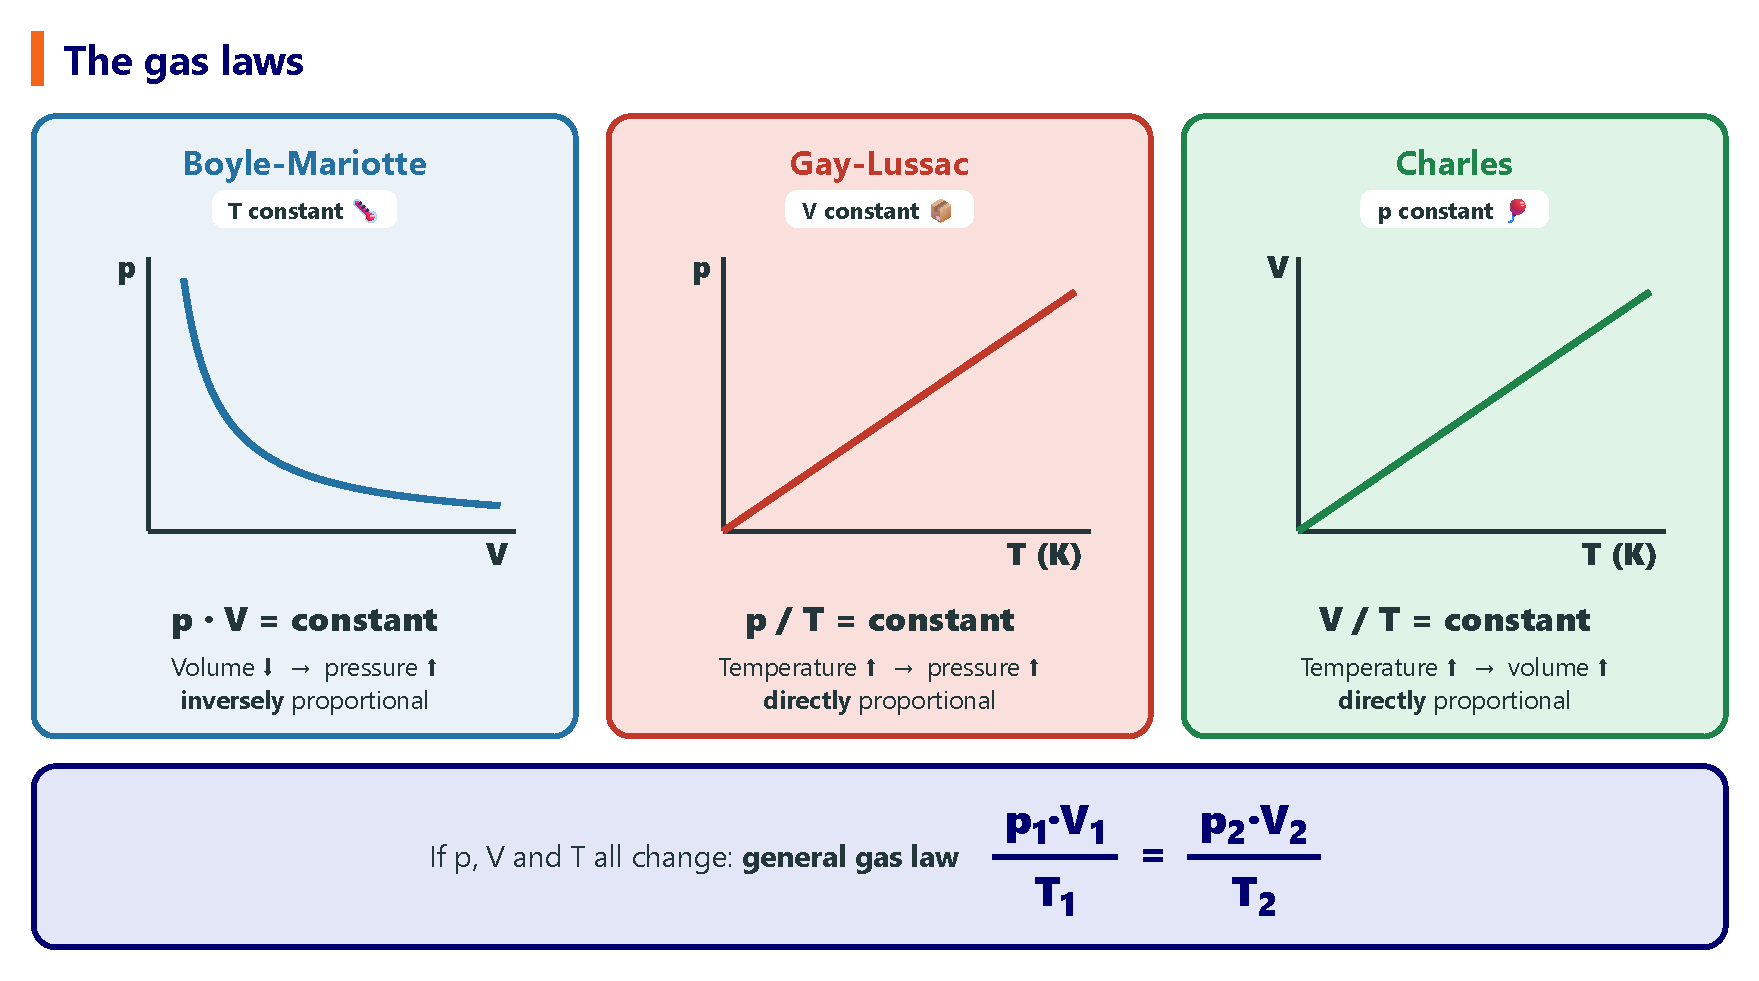
\includegraphics[width=\textwidth]{FigurasSVG/Unit_2_State_of_Matter/pdf/gas_laws.pdf}
    \caption{The three gas laws and the general gas law.}
    \label{fig:u2_gas_laws}
\end{figure}

\begin{table}[H]
    \centering
    \renewcommand{\arraystretch}{2}
    \begin{tabular}{lccc}
        \toprule
        \textbf{Law} & \textbf{Constant} & \textbf{Equation} & \textbf{Relationship} \\
        \midrule
        Boyle-Mariotte & \(T\) & \(p_1 \cdot V_1 = p_2 \cdot V_2\) & inversely proportional \\
        Gay-Lussac & \(V\) & \(\dfrac{p_1}{T_1} = \dfrac{p_2}{T_2}\) & directly proportional \\
        Charles & \(p\) & \(\dfrac{V_1}{T_1} = \dfrac{V_2}{T_2}\) & directly proportional \\
        \bottomrule
    \end{tabular}
    \caption{The gas laws.}
    \label{tab:u2_gas_laws}
\end{table}

\begin{impt}
    \negsubro{How do we know which law to use?} We look for the quantity that does \textbf{not} change (the one that stays \textbf{constant}):
    \begin{itemize}
        \item \(T\) constant \(\to\) \textbf{Boyle-Mariotte's law}.
        \item \(V\) constant \(\to\) \textbf{Gay-Lussac's law}.
        \item \(p\) constant \(\to\) \textbf{Charles' law}.
    \end{itemize}
    The complete method, step by step, is in the section \emph{Gas-law exercises}.
\end{impt}

%------------------------------------------------

\subsection{Boyle-Mariotte's law (constant temperature)}

\negsubro{What does this law tell us?} Take a bicycle pump, block the hole with your finger and push the handle. The more you push (the \textbf{smaller the volume}), the harder the air pushes back against your hand (the \textbf{bigger the pressure}).

Why does this happen? If the temperature of a gas does not change, its particles keep moving at the same speed. When we \textbf{compress} the gas, the particles have less space, so they hit the walls of the container \textbf{more often}: the \textbf{pressure increases}. If we let the gas \textbf{expand}, the particles have more space, they hit the walls less often and the pressure \textbf{decreases}.

We say that pressure and volume are \textbf{inversely proportional}: when one goes \textbf{up}, the other goes \textbf{down}. If the volume becomes half, the pressure becomes double; if the volume becomes double, the pressure becomes half.

\begin{definition}[Boyle-Mariotte's law]
    At constant temperature, the product of the pressure and the volume of a gas stays constant:
    \begin{equation*}
        p_1 \cdot V_1 = p_2 \cdot V_2
    \end{equation*}
\end{definition}

\begin{figure}[H]
    \centering
    % [FIGURA ORIGINAL] \includegraphics[width=\textwidth]{Unit_2/boyle_law}
    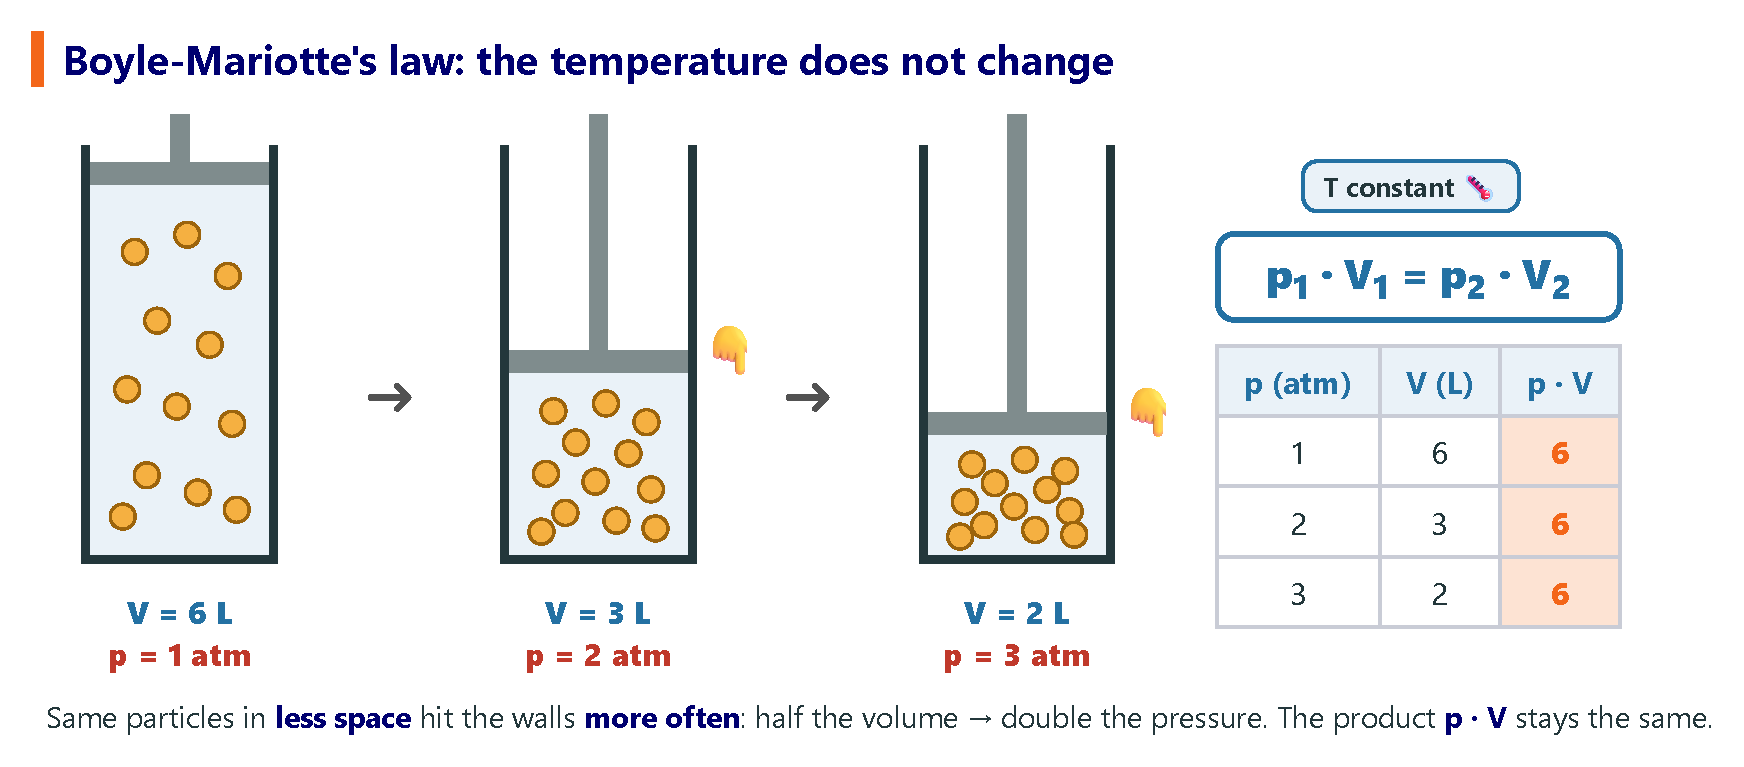
\includegraphics[width=\textwidth]{FigurasSVG/Unit_2_State_of_Matter/pdf/boyle_law.pdf}
    \caption{Boyle-Mariotte's law: at constant temperature, when the volume decreases the pressure increases, and \(p \cdot V\) stays the same.}
    \label{fig:u2_boyle_law}
\end{figure}

\begin{example}
    \textbf{In a \qty{3}{\litre} container, a gas exerts a pressure of \qty{2}{\atmospher} at \qty{60}{\celsius}. What will its volume be if the pressure doubles to \qty{4}{\atmospher} and the temperature stays the same?}
    \begin{enumerate}[label=\numberballmDarkTeal]
        \item Data: \(p_1 = \qty{2}{\atmospher}\), \(V_1 = \qty{3}{\litre}\), \(p_2 = \qty{4}{\atmospher}\). Unknown: \(\underline{V_2}\).
        \item \(T\) is constant \(\to\) \textbf{Boyle-Mariotte law}: \(p_1 \cdot V_1 = p_2 \cdot V_2\).
        \item We isolate \(V_2\) and calculate:
        \(\;V_2 = \dfrac{p_1 \cdot V_1}{p_2} = \dfrac{\qty{2}{\atmospher} \cdot \qty{3}{\litre}}{\qty{4}{\atmospher}} = \textcolor{red}{\qty{1.5}{\litre}}\)
    \end{enumerate}
    Pressure doubles, so volume halves: it makes sense!
\end{example}

\begin{exercise}
    In a \qty{3}{\litre} container, nitrogen exerts a pressure of \qty{4}{\atmospher}. What will the pressure be if the volume of the container doubles and the temperature stays the same?
    \begin{solu}
        \(T\) constant \(\to\) Boyle-Mariotte law: \(p_1 \cdot V_1 = p_2 \cdot V_2\). \\
        \(p_2 = \dfrac{p_1 \cdot V_1}{V_2} = \dfrac{\qty{4}{\atmospher} \cdot \qty{3}{\litre}}{\qty{6}{\litre}} = \qty{2}{\atmospher}\).
    \end{solu}
\end{exercise}

\begin{exercise}
    \qty{22.5}{\litre} of nitrogen at \qty{748}{\mmhg} are compressed until the pressure is \qty{725}{\mmhg}, at constant temperature. What is the new volume?
    \begin{solu}
        \(T\) constant \(\to\) Boyle-Mariotte law: \(p_1 \cdot V_1 = p_2 \cdot V_2\). \\
        \(V_2 = \dfrac{p_1 \cdot V_1}{p_2} = \dfrac{\qty{748}{\mmhg} \cdot \qty{22.5}{\litre}}{\qty{725}{\mmhg}} \approx \qty{23.2}{\litre}\).
    \end{solu}
\end{exercise}

\subsubsection{How to isolate each quantity in Boyle-Mariotte's law}

In an exercise the unknown can be any of the four quantities. We always start from the law, \(p_1 \cdot V_1 = p_2 \cdot V_2\), and leave the unknown \textbf{alone}. As we did with density, we do the \textbf{same operation on both sides}: if the unknown is \textbf{multiplied} by a quantity, we \textbf{divide} both sides by that quantity (or, with the shortcut, what is \textbf{multiplying} goes to the other side \textbf{dividing}).

\begin{figure}[H]
    \centering
    % [FIGURA ORIGINAL] \includegraphics[width=\textwidth]{Unit_2/boyle_isolate}
    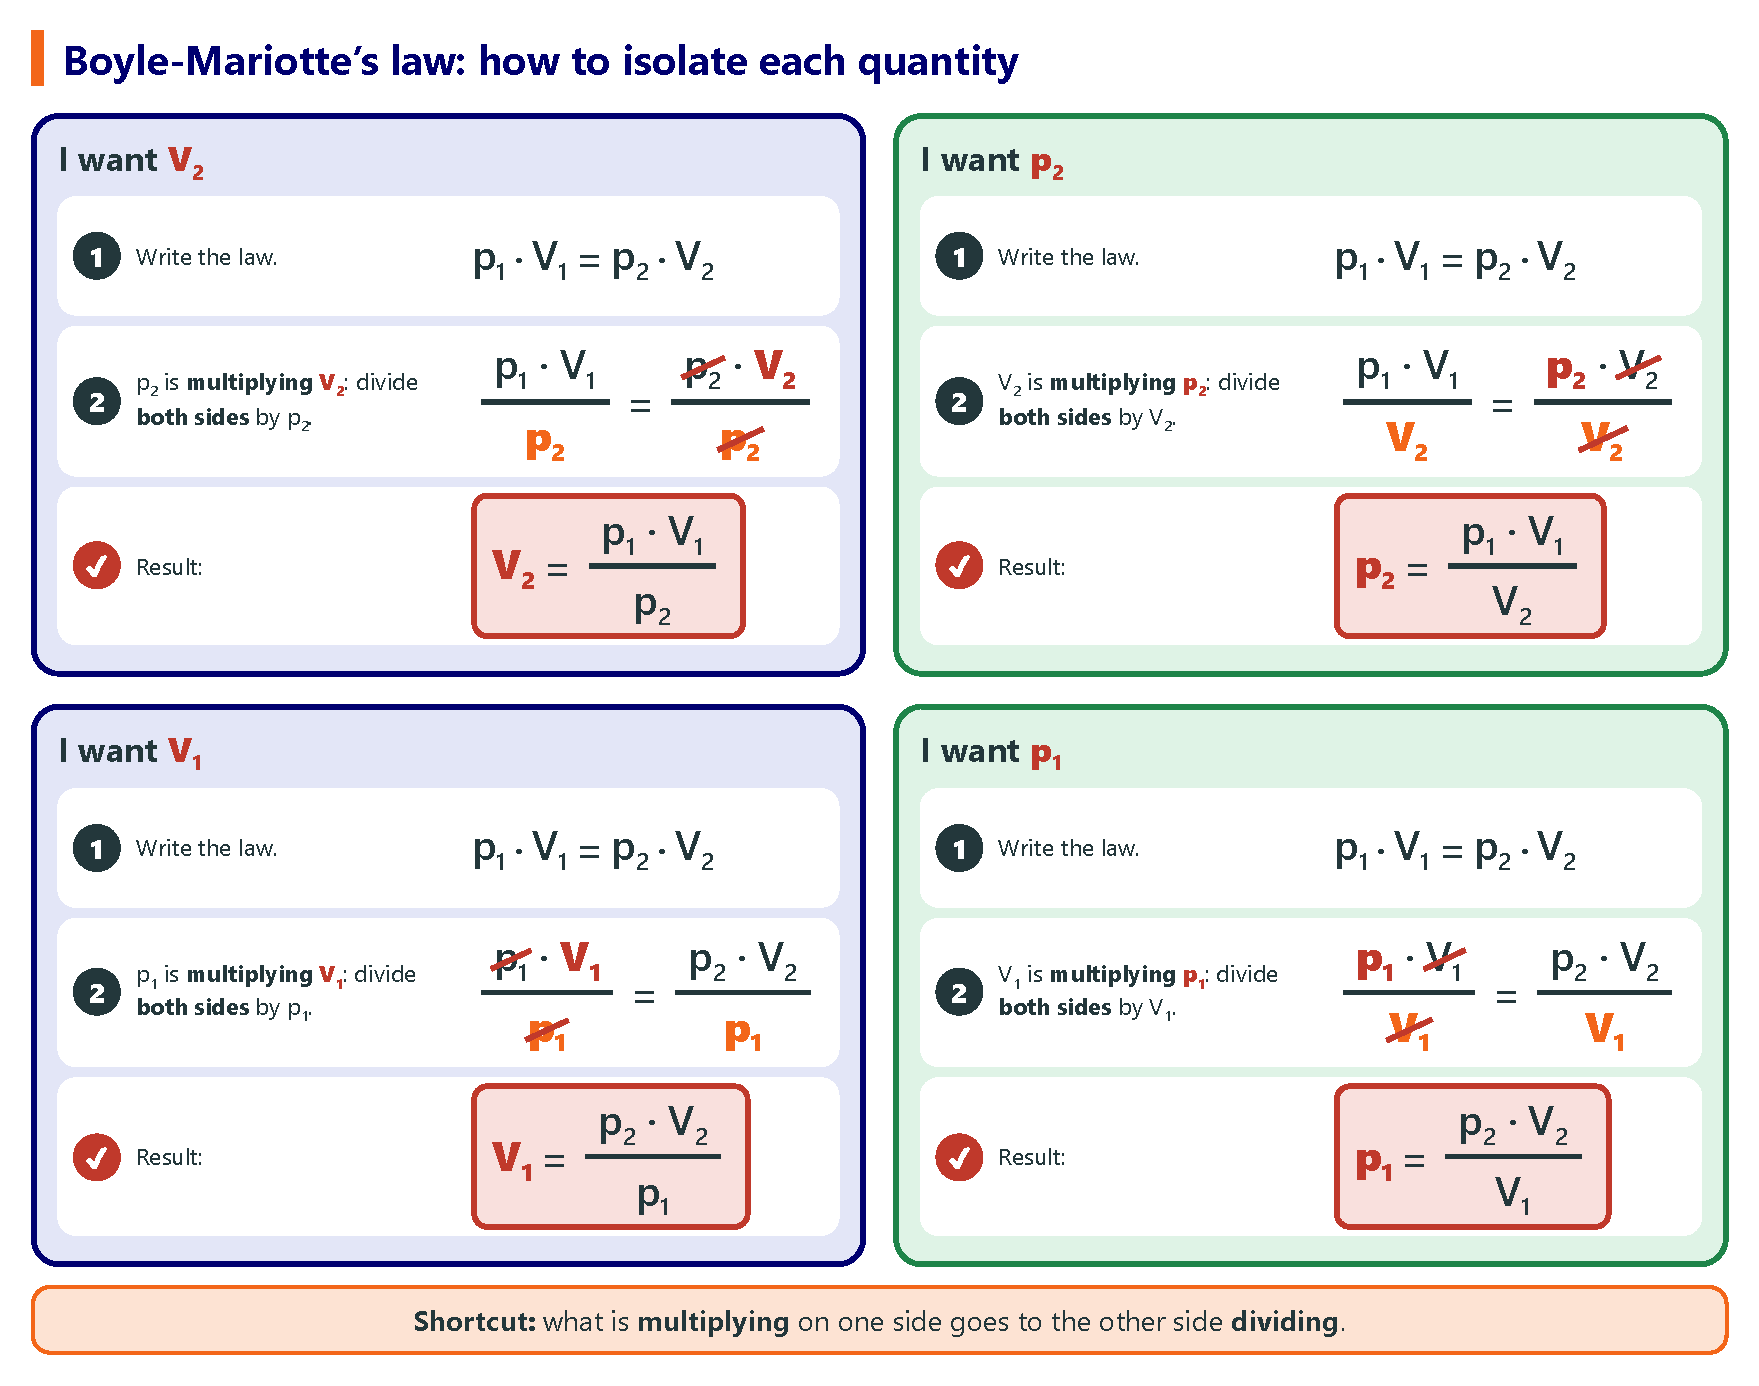
\includegraphics[width=\textwidth]{FigurasSVG/Unit_2_State_of_Matter/pdf/boyle_isolate.pdf}
    \caption{Isolating \(V_2\), \(p_2\), \(V_1\) and \(p_1\) in Boyle-Mariotte's law, step by step.}
    \label{fig:u2_boyle_isolate}
\end{figure}

\begin{itemize}
    \item \textbf{Unknown \(V_2\)}: \(p_2\) is multiplying \(V_2\), so we divide both sides by \(p_2\):
    \(\;\dfrac{p_1 \cdot V_1}{p_2} = \dfrac{\cancelred{p_2} \cdot V_2}{\cancelred{p_2}} \;\Rightarrow\; \textcolor{red}{V_2 = \dfrac{p_1 \cdot V_1}{p_2}}\)
    \item \textbf{Unknown \(p_2\)}: \(V_2\) is multiplying \(p_2\), so we divide both sides by \(V_2\):
    \(\;\dfrac{p_1 \cdot V_1}{V_2} = \dfrac{p_2 \cdot \cancelred{V_2}}{\cancelred{V_2}} \;\Rightarrow\; \textcolor{red}{p_2 = \dfrac{p_1 \cdot V_1}{V_2}}\)
    \item \textbf{Unknown \(V_1\)}: \(p_1\) is multiplying \(V_1\), so we divide both sides by \(p_1\):
    \(\;\dfrac{\cancelred{p_1} \cdot V_1}{\cancelred{p_1}} = \dfrac{p_2 \cdot V_2}{p_1} \;\Rightarrow\; \textcolor{red}{V_1 = \dfrac{p_2 \cdot V_2}{p_1}}\)
    \item \textbf{Unknown \(p_1\)}: \(V_1\) is multiplying \(p_1\), so we divide both sides by \(V_1\):
    \(\;\dfrac{p_1 \cdot \cancelred{V_1}}{\cancelred{V_1}} = \dfrac{p_2 \cdot V_2}{V_1} \;\Rightarrow\; \textcolor{red}{p_1 = \dfrac{p_2 \cdot V_2}{V_1}}\)
\end{itemize}

%------------------------------------------------

\subsection{Gay-Lussac's law (constant volume)}

\negsubro{What does this law tell us?} Have you noticed that spray cans have a warning: ``Do not leave in the sun or near a fire''? The can is made of metal, so the gas inside cannot change its volume. If it gets \textbf{hot}, the \textbf{pressure} of the gas \textbf{increases} so much that the can could explode.

Why does this happen? If a gas is inside a closed, rigid container, its volume cannot change. When we \textbf{heat} it, its particles move \textbf{faster} and hit the walls \textbf{harder and more often}: the \textbf{pressure increases}. When we cool it, the particles move more slowly and the pressure decreases.

We say that pressure and temperature (in kelvin) are \textbf{directly proportional}: when one goes \textbf{up}, the other goes \textbf{up} too. If the temperature in kelvin doubles, the pressure doubles too.

\begin{definition}[Gay-Lussac's law]
    At constant volume, the pressure of a gas divided by its temperature in kelvin stays constant:
    \begin{equation*}
        \dfrac{p_1}{T_1} = \dfrac{p_2}{T_2}
    \end{equation*}
\end{definition}

\begin{figure}[H]
    \centering
    % [FIGURA ORIGINAL] \includegraphics[width=\textwidth]{Unit_2/gay_lussac_law}
    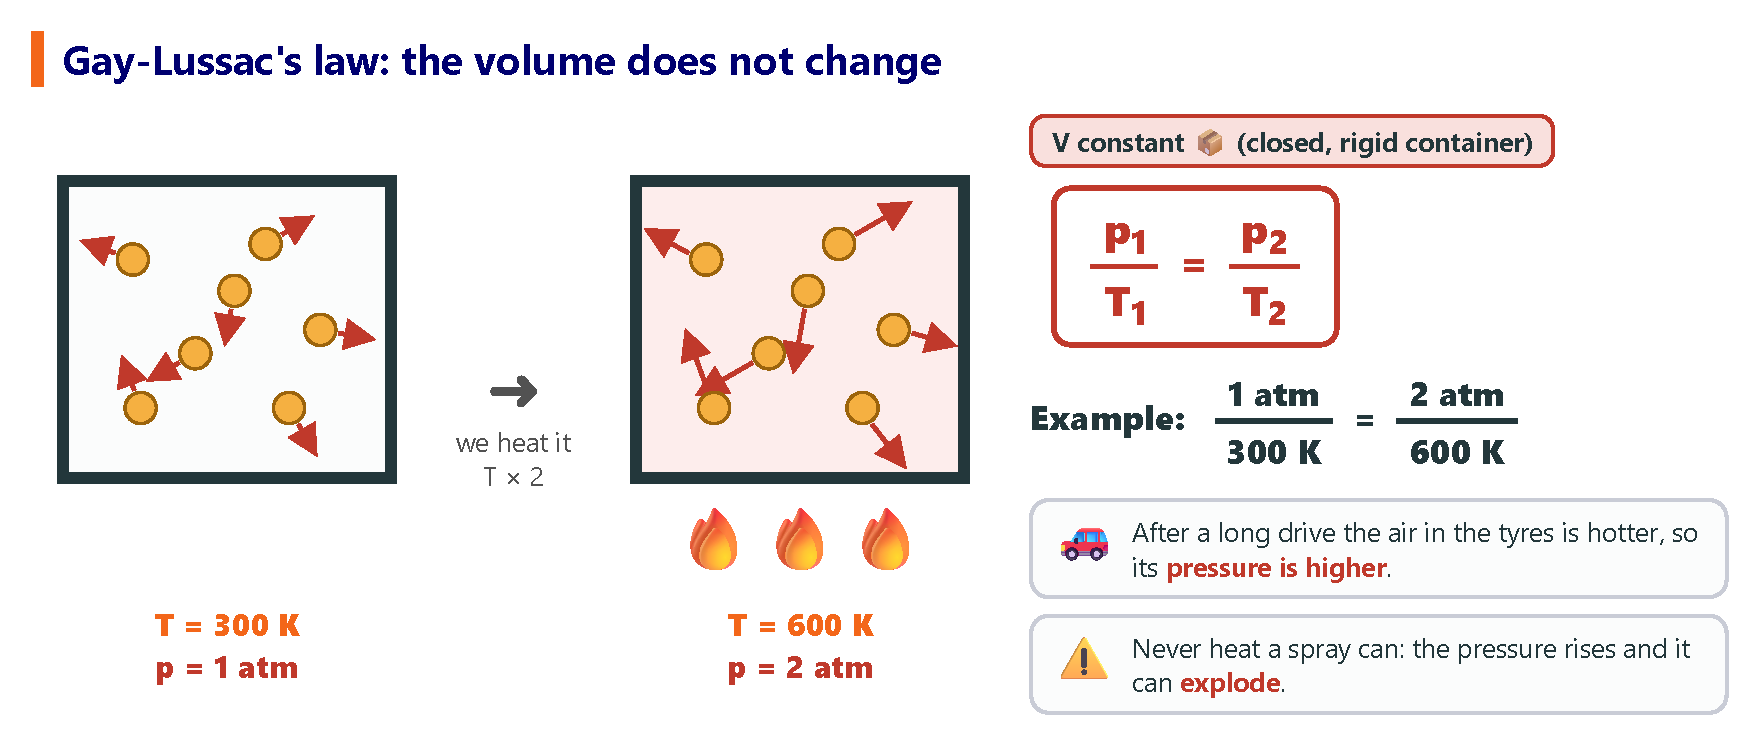
\includegraphics[width=\textwidth]{FigurasSVG/Unit_2_State_of_Matter/pdf/gay_lussac_law.pdf}
    \caption{Gay-Lussac's law: in a rigid container, if the temperature in kelvin doubles, the pressure doubles too.}
    \label{fig:u2_gay_lussac_law}
\end{figure}

\begin{example}
    \textbf{A closed container of gas is initially at \qty{0.500}{\atmospher} and \qty{25.0}{\celsius}. What will the pressure be at \qty{125.0}{\celsius}?}
    \begin{enumerate}[label=\numberballmDarkTeal]
        \item Data: \(p_1 = \qty{0.500}{\atmospher}\), \(T_1 = 25 + 273 = \qty{298}{\kelvin}\), \(T_2 = 125 + 273 = \qty{398}{\kelvin}\). Unknown: \(\underline{p_2}\).
        \item The container is closed, so \(V\) is constant \(\to\) \textbf{Gay-Lussac's law}: \(\dfrac{p_1}{T_1} = \dfrac{p_2}{T_2}\).
        \item We isolate \(p_2\) and calculate:
        \(\;p_2 = \dfrac{p_1 \cdot T_2}{T_1} = \dfrac{\qty{0.500}{\atmospher} \cdot \qty{398}{\kelvin}}{\qty{298}{\kelvin}} \approx \textcolor{red}{\qty{0.668}{\atmospher}}\)
    \end{enumerate}
    The temperature rises, so the pressure rises too: it makes sense!
\end{example}

\begin{exercise}
    In a \qty{10}{\litre} container, oxygen exerts a pressure of \qty{4}{\atmospher} at \qty{20}{\celsius}. What will the pressure be if the temperature rises to \qty{40}{\celsius} and the volume stays the same?
    \begin{solu}
        \(V\) constant \(\to\) Gay-Lussac's law: \(\dfrac{p_1}{T_1} = \dfrac{p_2}{T_2}\). \\
        In kelvin: \(T_1 = 20 + 273 = \qty{293}{\kelvin}\); \(T_2 = 40 + 273 = \qty{313}{\kelvin}\). \\
        \(p_2 = \dfrac{p_1 \cdot T_2}{T_1} = \dfrac{\qty{4}{\atmospher} \cdot \qty{313}{\kelvin}}{\qty{293}{\kelvin}} \approx \qty{4.27}{\atmospher}\).
    \end{solu}
\end{exercise}

\begin{exercise}
    A gas is cooled from \qty{323}{\kelvin} to \qty{273}{\kelvin} and its volume is kept constant. What is the final pressure if the original pressure was \qty{750.0}{\mmhg}?
    \begin{solu}
        \(V\) constant \(\to\) Gay-Lussac's law: \(\dfrac{p_1}{T_1} = \dfrac{p_2}{T_2}\). \\
        \(p_2 = \dfrac{p_1 \cdot T_2}{T_1} = \dfrac{\qty{750.0}{\mmhg} \cdot \qty{273}{\kelvin}}{\qty{323}{\kelvin}} \approx \qty{634}{\mmhg}\).
    \end{solu}
\end{exercise}

\subsubsection{How to isolate each quantity in Gay-Lussac's law}

We always start from the law, \(\dfrac{p_1}{T_1} = \dfrac{p_2}{T_2}\). Here the quantities are inside fractions, so we do it in two steps:
\begin{enumerate}[label=\numberballmDarkTeal]
    \item \textbf{We remove the fractions (cross-multiplication).} \(T_1\) is \textbf{dividing} on the left, so it goes to the right \textbf{multiplying}; \(T_2\) is \textbf{dividing} on the right, so it goes to the left \textbf{multiplying}:
    \begin{equation*}
        \dfrac{p_1}{T_1} = \dfrac{p_2}{T_2} \quad\Longrightarrow\quad p_1 \cdot T_2 = p_2 \cdot T_1
    \end{equation*}
    \item \textbf{We isolate the unknown}: the quantity that is \textbf{multiplying} the unknown goes to the other side \textbf{dividing} (we divide both sides by it).
\end{enumerate}

\begin{figure}[H]
    \centering
    % [FIGURA ORIGINAL] \includegraphics[width=\textwidth]{Unit_2/gay_lussac_isolate}
    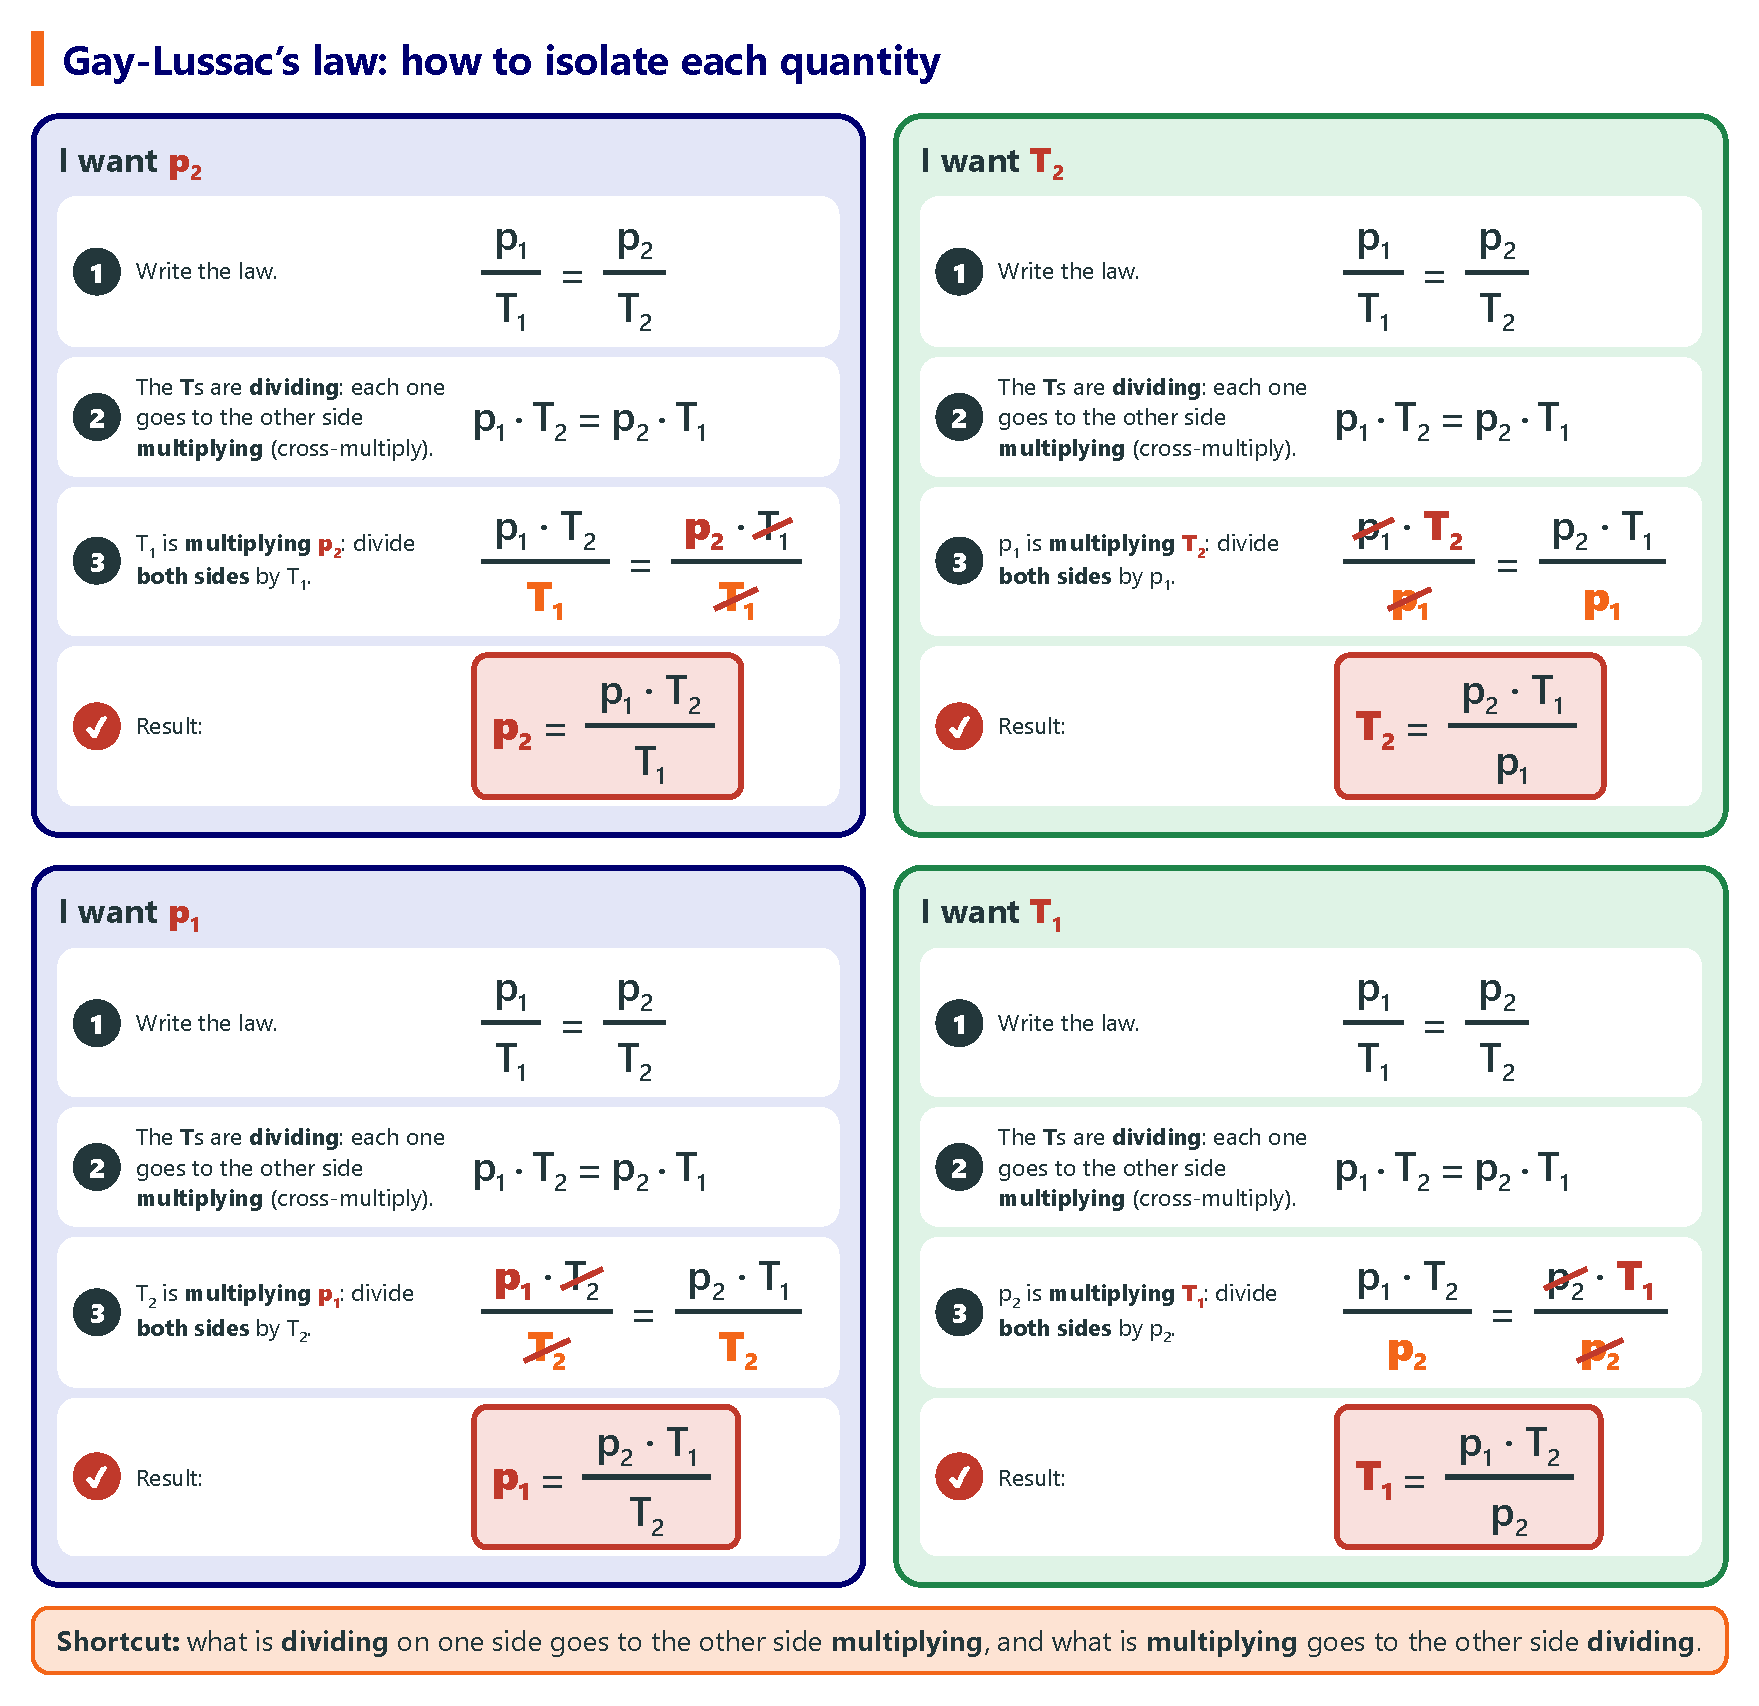
\includegraphics[width=\textwidth]{FigurasSVG/Unit_2_State_of_Matter/pdf/gay_lussac_isolate.pdf}
    \caption{Isolating the four quantities in Gay-Lussac's law, step by step.}
    \label{fig:u2_gay_lussac_isolate}
\end{figure}

Starting from \(p_1 \cdot T_2 = p_2 \cdot T_1\):
\begin{itemize}
    \item \textbf{Unknown \(p_2\)}: we divide both sides by \(T_1\):
    \(\;\dfrac{p_1 \cdot T_2}{T_1} = \dfrac{p_2 \cdot \cancelred{T_1}}{\cancelred{T_1}} \;\Rightarrow\; \textcolor{red}{p_2 = \dfrac{p_1 \cdot T_2}{T_1}}\)
    \item \textbf{Unknown \(T_2\)}: we divide both sides by \(p_1\):
    \(\;\dfrac{\cancelred{p_1} \cdot T_2}{\cancelred{p_1}} = \dfrac{p_2 \cdot T_1}{p_1} \;\Rightarrow\; \textcolor{red}{T_2 = \dfrac{p_2 \cdot T_1}{p_1}}\)
    \item \textbf{Unknown \(p_1\)}: we divide both sides by \(T_2\):
    \(\;\dfrac{p_1 \cdot \cancelred{T_2}}{\cancelred{T_2}} = \dfrac{p_2 \cdot T_1}{T_2} \;\Rightarrow\; \textcolor{red}{p_1 = \dfrac{p_2 \cdot T_1}{T_2}}\)
    \item \textbf{Unknown \(T_1\)}: we divide both sides by \(p_2\):
    \(\;\dfrac{p_1 \cdot T_2}{p_2} = \dfrac{\cancelred{p_2} \cdot T_1}{\cancelred{p_2}} \;\Rightarrow\; \textcolor{red}{T_1 = \dfrac{p_1 \cdot T_2}{p_2}}\)
\end{itemize}

%------------------------------------------------

\subsection{Charles' law (constant pressure)}

\negsubro{What does this law tell us?} Blow up a balloon and put it in the freezer: after a while it looks smaller and wrinkled. Take it out and leave it in the sun: it becomes big again. The \textbf{colder} the gas, the \textbf{smaller its volume}; the \textbf{hotter} the gas, the \textbf{bigger its volume}.

Why does this happen? Here the pressure of the gas does not change (a balloon or a syringe whose plunger can move freely). When we \textbf{heat} the gas, its particles move \textbf{faster} and push the walls \textbf{outwards}: the gas \textbf{expands} (its volume increases). When we cool it, the particles move more slowly and the gas \textbf{contracts}.

We say that volume and temperature (in kelvin) are \textbf{directly proportional}: when one goes \textbf{up}, the other goes \textbf{up} too. If the temperature in kelvin doubles, the volume doubles too.

\begin{definition}[Charles' law]
    At constant pressure, the volume of a gas divided by its temperature in kelvin stays constant:
    \begin{equation*}
        \dfrac{V_1}{T_1} = \dfrac{V_2}{T_2}
    \end{equation*}
\end{definition}

\begin{figure}[H]
    \centering
    % [FIGURA ORIGINAL] \includegraphics[width=\textwidth]{Unit_2/charles_law}
    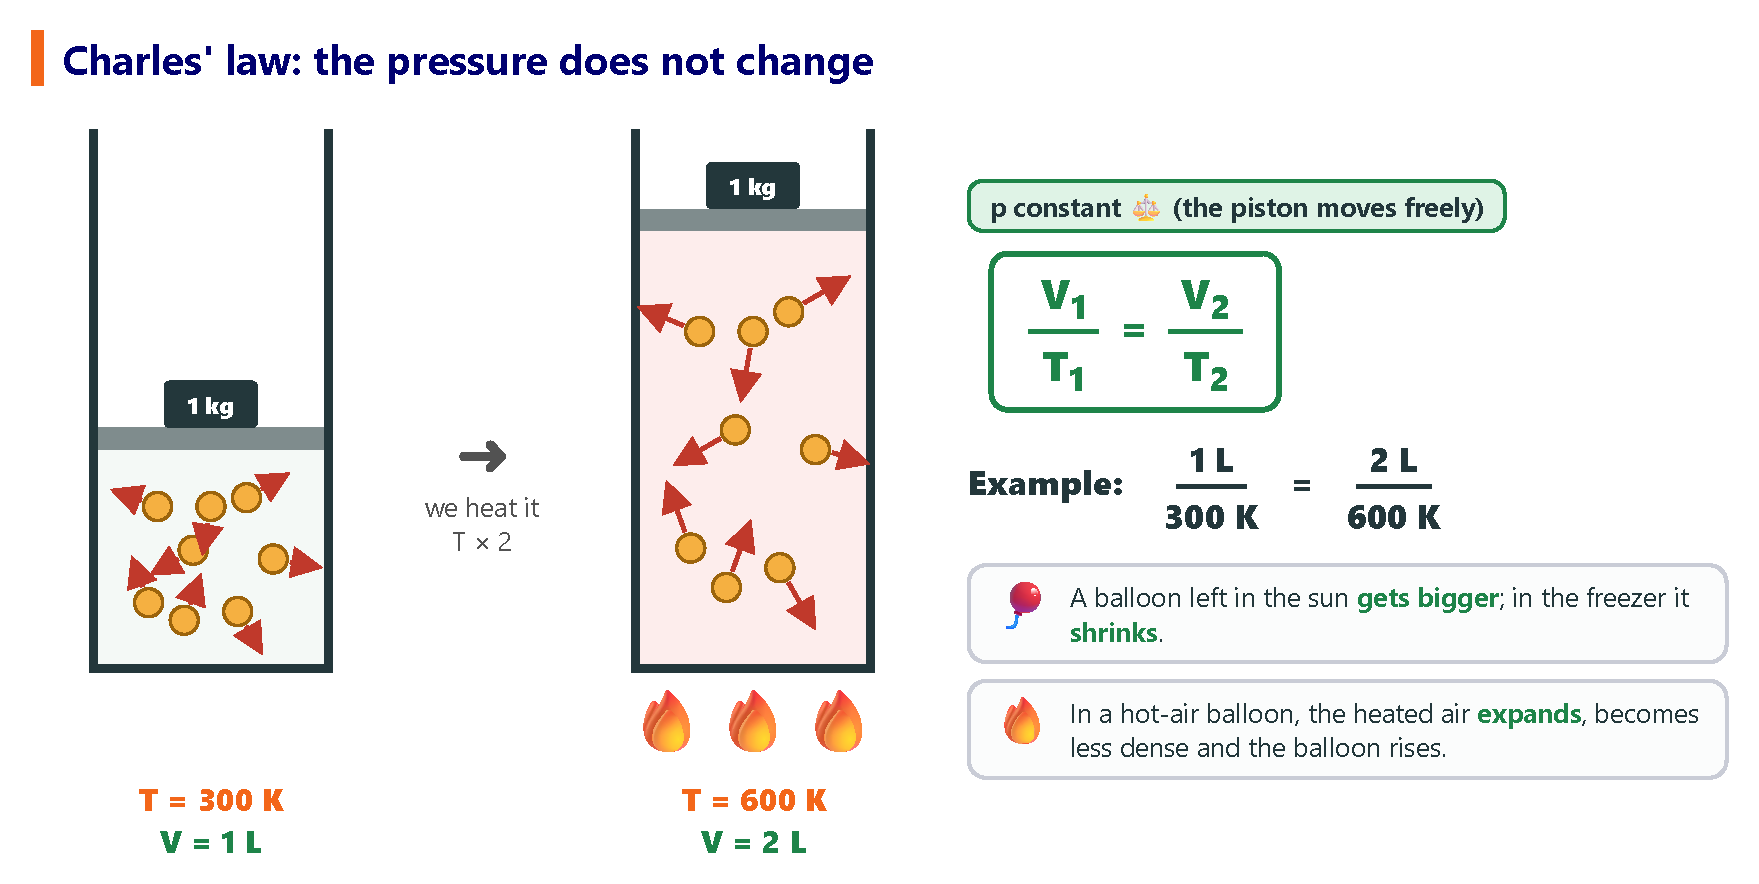
\includegraphics[width=\textwidth]{FigurasSVG/Unit_2_State_of_Matter/pdf/charles_law.pdf}
    \caption{Charles' law: with a free piston the pressure stays the same, and if the temperature in kelvin doubles, the volume doubles too.}
    \label{fig:u2_charles_law}
\end{figure}

\begin{example}
    \textbf{A gas occupies \qty{900.0}{\mL} at \qty{27.0}{\celsius}. What is its volume at \qty{132.0}{\celsius} if the pressure does not change?}
    \begin{enumerate}[label=\numberballmDarkTeal]
        \item Data: \(V_1 = \qty{900.0}{\mL}\), \(T_1 = 27 + 273 = \qty{300}{\kelvin}\), \(T_2 = 132 + 273 = \qty{405}{\kelvin}\). Unknown: \(\underline{V_2}\).
        \item \(p\) is constant \(\to\) \textbf{Charles' law}: \(\dfrac{V_1}{T_1} = \dfrac{V_2}{T_2}\).
        \item We isolate \(V_2\) and calculate:
        \(\;V_2 = \dfrac{V_1 \cdot T_2}{T_1} = \dfrac{\qty{900.0}{\mL} \cdot \qty{405}{\kelvin}}{\qty{300}{\kelvin}} = \textcolor{red}{\qty{1215}{\mL}}\)
    \end{enumerate}
    The temperature rises, so the gas expands: it makes sense!
\end{example}

\begin{exercise}
    A gas occupies \qty{2}{\litre} at \qty{300}{\kelvin}. What volume will it occupy if the temperature rises to \qty{450}{\kelvin}, with the pressure unchanged?
    \begin{solu}
        \(p\) constant \(\to\) Charles' law: \(\dfrac{V_1}{T_1} = \dfrac{V_2}{T_2}\). \\
        \(V_2 = \dfrac{V_1 \cdot T_2}{T_1} = \dfrac{\qty{2}{\litre} \cdot \qty{450}{\kelvin}}{\qty{300}{\kelvin}} = \qty{3}{\litre}\).
    \end{solu}
\end{exercise}

\begin{exercise}
    \qty{5.00}{\litre} of a gas are collected at \qty{100}{\kelvin} and then allowed to expand to \qty{20.0}{\litre}. What must the new temperature be to keep the same pressure?
    \begin{solu}
        \(p\) constant \(\to\) Charles' law: \(\dfrac{V_1}{T_1} = \dfrac{V_2}{T_2}\). \\
        \(T_2 = \dfrac{V_2 \cdot T_1}{V_1} = \dfrac{\qty{20.0}{\litre} \cdot \qty{100}{\kelvin}}{\qty{5.00}{\litre}} = \qty{400}{\kelvin}\).
    \end{solu}
\end{exercise}

\subsubsection{How to isolate each quantity in Charles' law}

We always start from the law, \(\dfrac{V_1}{T_1} = \dfrac{V_2}{T_2}\). Here the quantities are inside fractions, so we do it in two steps:
\begin{enumerate}[label=\numberballmDarkTeal]
    \item \textbf{We remove the fractions (cross-multiplication).} \(T_1\) is \textbf{dividing} on the left, so it goes to the right \textbf{multiplying}; \(T_2\) is \textbf{dividing} on the right, so it goes to the left \textbf{multiplying}:
    \begin{equation*}
        \dfrac{V_1}{T_1} = \dfrac{V_2}{T_2} \quad\Longrightarrow\quad V_1 \cdot T_2 = V_2 \cdot T_1
    \end{equation*}
    \item \textbf{We isolate the unknown}: the quantity that is \textbf{multiplying} the unknown goes to the other side \textbf{dividing} (we divide both sides by it).
\end{enumerate}

\begin{figure}[H]
    \centering
    % [FIGURA ORIGINAL] \includegraphics[width=\textwidth]{Unit_2/charles_isolate}
    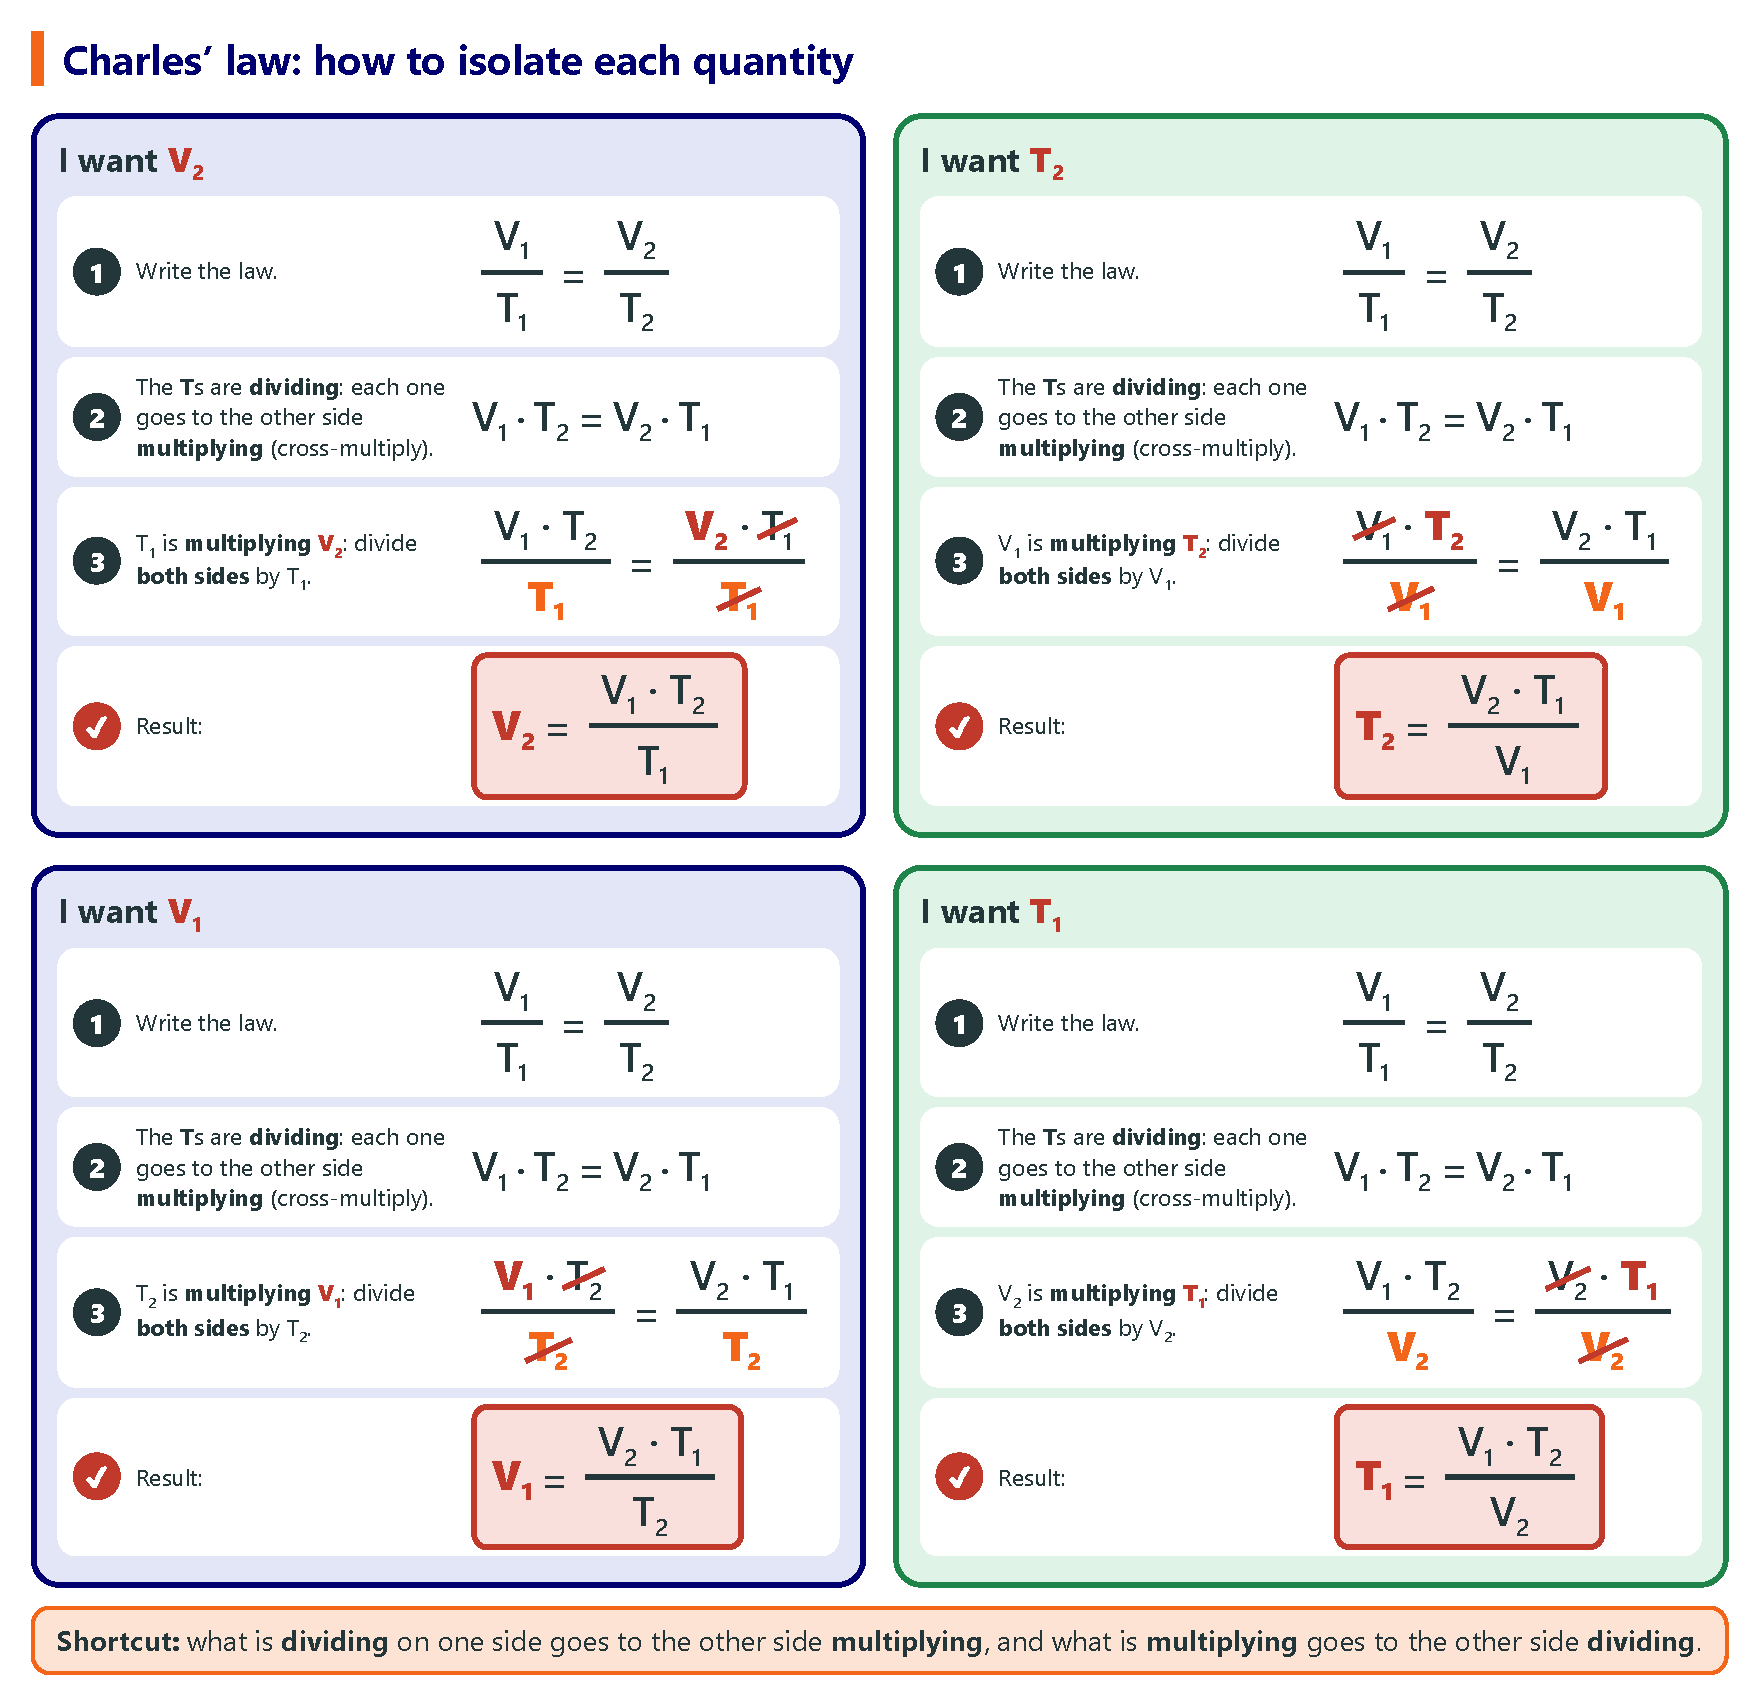
\includegraphics[width=\textwidth]{FigurasSVG/Unit_2_State_of_Matter/pdf/charles_isolate.pdf}
    \caption{Isolating the four quantities in Charles' law, step by step.}
    \label{fig:u2_charles_isolate}
\end{figure}

Starting from \(V_1 \cdot T_2 = V_2 \cdot T_1\):
\begin{itemize}
    \item \textbf{Unknown \(V_2\)}: we divide both sides by \(T_1\):
    \(\;\dfrac{V_1 \cdot T_2}{T_1} = \dfrac{V_2 \cdot \cancelred{T_1}}{\cancelred{T_1}} \;\Rightarrow\; \textcolor{red}{V_2 = \dfrac{V_1 \cdot T_2}{T_1}}\)
    \item \textbf{Unknown \(T_2\)}: we divide both sides by \(V_1\):
    \(\;\dfrac{\cancelred{V_1} \cdot T_2}{\cancelred{V_1}} = \dfrac{V_2 \cdot T_1}{V_1} \;\Rightarrow\; \textcolor{red}{T_2 = \dfrac{V_2 \cdot T_1}{V_1}}\)
    \item \textbf{Unknown \(V_1\)}: we divide both sides by \(T_2\):
    \(\;\dfrac{V_1 \cdot \cancelred{T_2}}{\cancelred{T_2}} = \dfrac{V_2 \cdot T_1}{T_2} \;\Rightarrow\; \textcolor{red}{V_1 = \dfrac{V_2 \cdot T_1}{T_2}}\)
    \item \textbf{Unknown \(T_1\)}: we divide both sides by \(V_2\):
    \(\;\dfrac{V_1 \cdot T_2}{V_2} = \dfrac{\cancelred{V_2} \cdot T_1}{\cancelred{V_2}} \;\Rightarrow\; \textcolor{red}{T_1 = \dfrac{V_1 \cdot T_2}{V_2}}\)
\end{itemize}

%------------------------------------------------

\subsection{Gas-law exercises}

In these exercises the laws are mixed. To solve them correctly, always follow the same procedure:

\negsubro{Method, step by step}:
\begin{enumerate}[label=\numberballmDarkTeal]
    \item \textbf{Read} the exercise \textbf{once}, to understand what is happening.
    \item \textbf{Read} the exercise \textbf{a second time}, looking for the numbers and their units.
    \item Draw a \textbf{table} with two columns: \textbf{Data} and \textbf{Unknown}.
    \item Write the \textbf{data} that the exercise gives you, saying whether each one belongs to the \textbf{beginning (1)} or to the \textbf{end (2)}: \(p_1\), \(V_1\), \(T_1\), \(p_2\)\ldots{} Change the temperatures to \textbf{kelvin}.
    \item In the \textbf{Unknown} column, write what the exercise asks for.
    \item Find the quantity that stays \textbf{constant}. It tells you which law you have to use: write its \textbf{name}.
    \item Write the \textbf{formula} of that law.
    \item \textbf{Isolate} the unknown in the formula.
    \item \textbf{Substitute} the numbers of each quantity (with their units), \textbf{calculate}, and check that the result makes sense.
\end{enumerate}

\begin{figure}[H]
    \centering
    % [FIGURA ORIGINAL] \includegraphics[width=\textwidth]{Unit_2/gas_law_method}
    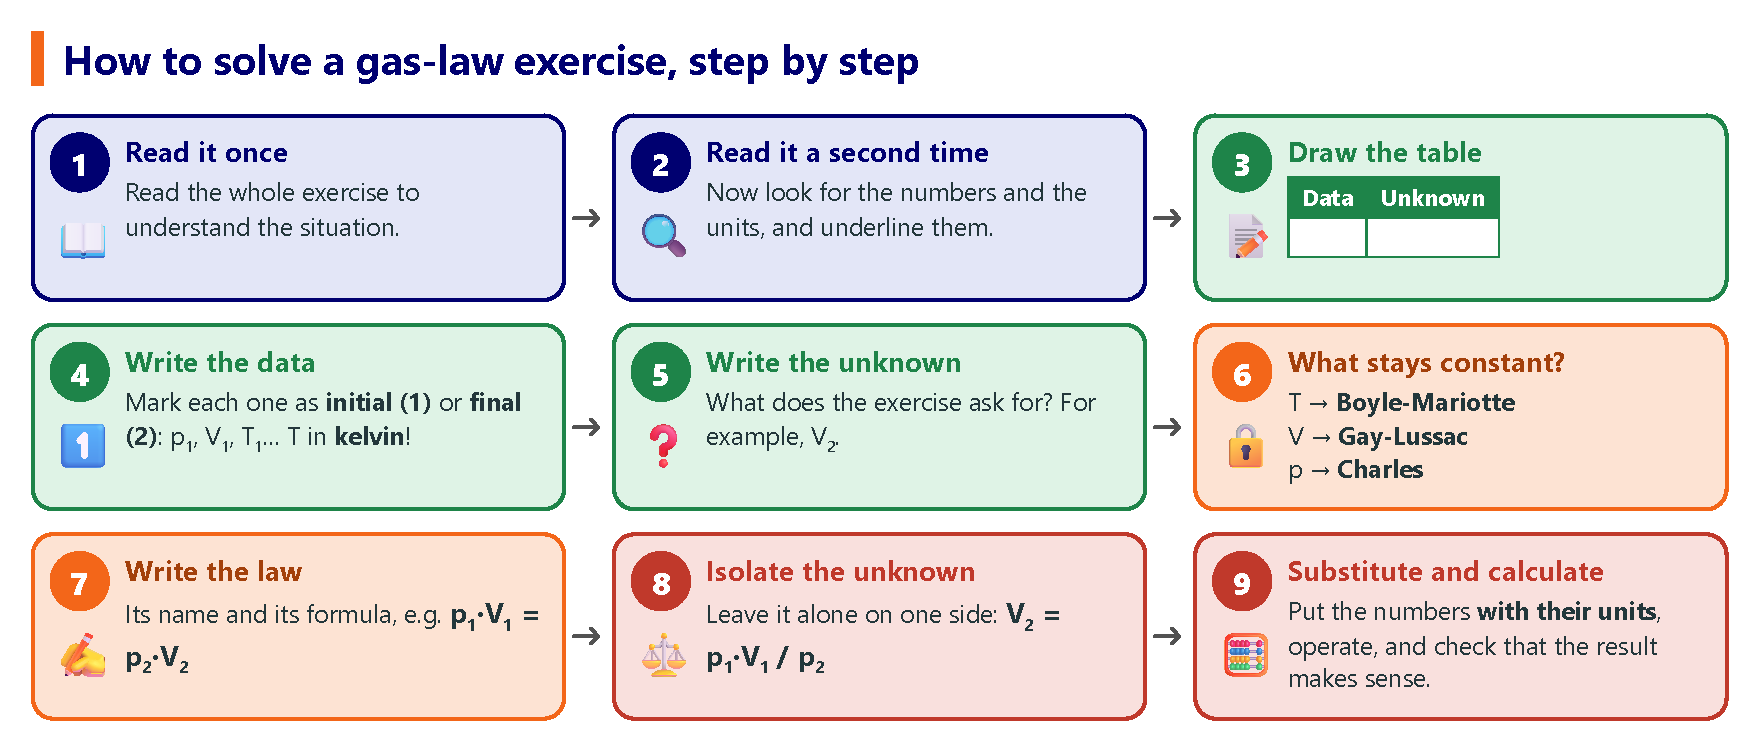
\includegraphics[width=\textwidth]{FigurasSVG/Unit_2_State_of_Matter/pdf/gas_law_method.pdf}
    \caption{The nine steps to solve a gas-law exercise.}
    \label{fig:u2_gas_law_method}
\end{figure}

\begin{example}
    \textbf{A gas occupies \qty{2.0}{\litre} at \qty{27}{\celsius}. It is heated to \qty{127}{\celsius} without changing its pressure. What is its final volume?}
    \begin{itemize}[leftmargin=2.3cm, labelwidth=2cm]
        \item[\textbf{Steps 1--2:}] We read the exercise twice: the gas is heated, and the pressure does not change.
        \item[\textbf{Steps 3--5:}] Table of data and unknown (temperatures in kelvin):
        \begin{center}
            \renewcommand{\arraystretch}{1.3}
            % --- tabla antigua ---
            % \begin{tabular}{l|l}
                % \textbf{Data} & \textbf{Unknown} \\
                % \hline
                % \(V_1 = \qty{2.0}{\litre}\) (beginning) & \(V_2 = \,?\) (end) \\
                % \(T_1 = 27 + 273 = \qty{300}{\kelvin}\) (beginning) & \\
                % \(T_2 = 127 + 273 = \qty{400}{\kelvin}\) (end) & \\
                % \(p\) = constant & \\
            % \end{tabular}
            % --- tabla nueva ---
            \begin{tabular}{@{}ll@{}}
                \toprule
                \textbf{Data} & \textbf{Unknown} \\
                \midrule
                \(V_1 = \qty{2.0}{\litre}\) (beginning) & \(V_2 = \,?\) (end) \\[3pt]
                \(T_1 = 27 + 273 = \qty{300}{\kelvin}\) (beginning) &  \\[3pt]
                \(T_2 = 127 + 273 = \qty{400}{\kelvin}\) (end) &  \\[3pt]
                \(p\) = constant &  \\
                \bottomrule
            \end{tabular}
        \end{center}
        \item[\textbf{Step 6:}] \(p\) is constant \(\to\) \textbf{Charles' law}.
        \item[\textbf{Step 7:}] Formula: \(\dfrac{V_1}{T_1} = \dfrac{V_2}{T_2}\).
        \item[\textbf{Step 8:}] We isolate \(V_2\): \(V_2 = \dfrac{V_1 \cdot T_2}{T_1}\).
        \item[\textbf{Step 9:}] \(V_2 = \dfrac{\qty{2.0}{\litre} \cdot \qty{400}{\kelvin}}{\qty{300}{\kelvin}} \approx \textcolor{red}{\qty{2.7}{\litre}}\). The gas is heated, so it expands: it makes sense!
    \end{itemize}
\end{example}

\begin{exercise}
    A gas with a volume of \qty{4}{\litre} at a pressure of \qty{205}{\kilo\pascal} is allowed to expand to a volume of \qty{12.0}{\litre}. What is the pressure in the container if the temperature remains constant?
    \begin{solu}
        \(T\) constant \(\to\) Boyle-Mariotte law. \\
        \(p_2 = \dfrac{p_1 \cdot V_1}{V_2} = \dfrac{\qty{205}{\kilo\pascal} \cdot \qty{4}{\litre}}{\qty{12.0}{\litre}} \approx \qty{68.3}{\kilo\pascal}\).
    \end{solu}
\end{exercise}

\begin{exercise}
    A closed, rigid gas container is initially at \qty{47}{\mmhg} and \qty{77}{\kelvin} (the temperature of liquid nitrogen). What will the pressure be when the container warms up to room temperature, \qty{25.0}{\celsius}?
    \begin{solu}
        \(V\) constant \(\to\) Gay-Lussac's law. \(T_2 = 25 + 273 = \qty{298}{\kelvin}\). \\
        \(p_2 = \dfrac{p_1 \cdot T_2}{T_1} = \dfrac{\qty{47}{\mmhg} \cdot \qty{298}{\kelvin}}{\qty{77}{\kelvin}} \approx \qty{182}{\mmhg}\).
    \end{solu}
\end{exercise}

\begin{exercise}
    \qty{15.0}{\litre} of neon at \qty{25.0}{\celsius} are allowed to expand to \qty{45.0}{\litre}. What must the new temperature be to keep the pressure constant?
    \begin{solu}
        \(p\) constant \(\to\) Charles' law. \(T_1 = 25 + 273 = \qty{298}{\kelvin}\). \\
        \(T_2 = \dfrac{V_2 \cdot T_1}{V_1} = \dfrac{\qty{45.0}{\litre} \cdot \qty{298}{\kelvin}}{\qty{15.0}{\litre}} = \qty{894}{\kelvin}\), that is, \(894 - 273 = \qty{621}{\celsius}\).
    \end{solu}
\end{exercise}

\begin{exercise}
    A gas at \qty{1.00}{\atmospher} is heated from \qty{20.0}{\celsius} to \qty{30.0}{\celsius} while its volume stays constant. Calculate the new pressure and how much the pressure has changed.
    \begin{solu}
        \(V\) constant \(\to\) Gay-Lussac's law. \(T_1 = 20 + 273 = \qty{293}{\kelvin}\); \(T_2 = 30 + 273 = \qty{303}{\kelvin}\). \\
        \(p_2 = \dfrac{p_1 \cdot T_2}{T_1} = \dfrac{\qty{1.00}{\atmospher} \cdot \qty{303}{\kelvin}}{\qty{293}{\kelvin}} \approx \qty{1.034}{\atmospher}\). \\
        The pressure increases by about \(\num{1.034} - \num{1.00} = \qty{0.034}{\atmospher}\).
    \end{solu}
\end{exercise}

\begin{exercise}
    A \qty{40}{\litre} tank of ammonia has a pressure of \qty{12.7}{\kilo\pascal}. Calculate the volume of the ammonia if its pressure changes to \qty{8.4}{\kilo\pascal} while its temperature remains constant.
    \begin{solu}
        \(T\) constant \(\to\) Boyle-Mariotte law. \\
        \(V_2 = \dfrac{p_1 \cdot V_1}{p_2} = \dfrac{\qty{12.7}{\kilo\pascal} \cdot \qty{40}{\litre}}{\qty{8.4}{\kilo\pascal}} \approx \qty{60.5}{\litre}\).
    \end{solu}
\end{exercise}

\begin{exercise}
    \qty{6.00}{\litre} of a gas at \qty{20.0}{\celsius} are compressed to \qty{4.00}{\litre} at constant pressure. Calculate the final temperature and how much the temperature has decreased.
    \begin{solu}
        \(p\) constant \(\to\) Charles' law. \(T_1 = 20 + 273 = \qty{293}{\kelvin}\). \\
        \(T_2 = \dfrac{V_2 \cdot T_1}{V_1} = \dfrac{\qty{4.00}{\litre} \cdot \qty{293}{\kelvin}}{\qty{6.00}{\litre}} \approx \qty{195}{\kelvin}\) (about \qty{-78}{\celsius}). \\
        The temperature decreases by about \(293 - 195 = \qty{98}{\kelvin}\), which is the same as \qty{98}{\celsius}, because a kelvin and a degree Celsius have the same size.
    \end{solu}
\end{exercise}

\begin{exercise}
    A gas thermometer measures temperature by measuring the pressure of a gas inside a container of fixed volume. The thermometer reads a pressure of \qty{248}{\kilo\pascal} at \qty{0}{\celsius}. What is the temperature when it reads a pressure of \qty{345}{\kilo\pascal}?
    \begin{solu}
        \(V\) constant \(\to\) Gay-Lussac's law. \(T_1 = 0 + 273 = \qty{273}{\kelvin}\). \\
        \(T_2 = \dfrac{p_2 \cdot T_1}{p_1} = \dfrac{\qty{345}{\kilo\pascal} \cdot \qty{273}{\kelvin}}{\qty{248}{\kilo\pascal}} \approx \qty{380}{\kelvin}\), that is, \(380 - 273 = \qty{107}{\celsius}\).
    \end{solu}
\end{exercise}

\begin{exercise}
    What pressure is needed to compress \qty{196.0}{\litre} of air at \qty{1.00}{\atmospher} into a cylinder whose volume is \qty{26}{\litre}, without changing its temperature?
    \begin{solu}
        \(T\) constant \(\to\) Boyle-Mariotte law. \\
        \(p_2 = \dfrac{p_1 \cdot V_1}{V_2} = \dfrac{\qty{1.00}{\atmospher} \cdot \qty{196.0}{\litre}}{\qty{26}{\litre}} \approx \qty{7.54}{\atmospher}\).
    \end{solu}
\end{exercise}

\begin{exercise}
    A gas is collected in a closed, rigid container at \qty{22.0}{\celsius} and \qty{745}{\mmhg}. When the temperature changes to \qty{0}{\celsius}, what is the new pressure?
    \begin{solu}
        \(V\) constant \(\to\) Gay-Lussac's law. \(T_1 = 22 + 273 = \qty{295}{\kelvin}\); \(T_2 = 0 + 273 = \qty{273}{\kelvin}\). \\
        \(p_2 = \dfrac{p_1 \cdot T_2}{T_1} = \dfrac{\qty{745}{\mmhg} \cdot \qty{273}{\kelvin}}{\qty{295}{\kelvin}} \approx \qty{689}{\mmhg}\).
    \end{solu}
\end{exercise}

\begin{exercise}
    A gas in a closed, rigid container has a pressure of \qty{699.0}{\mmhg} at \qty{40.0}{\celsius}. At what temperature will its pressure be \qty{1.00}{\atmospher}? (Remember: \(\qty{1}{\atmospher} = \qty{760}{\mmhg}\).)
    \begin{solu}
        \(V\) constant \(\to\) Gay-Lussac's law. \(T_1 = 40 + 273 = \qty{313}{\kelvin}\). \\
        Both pressures must be in the same unit: \(p_2 = \qty{1.00}{\atmospher} = \qty{760}{\mmhg}\). \\
        \(T_2 = \dfrac{p_2 \cdot T_1}{p_1} = \dfrac{\qty{760}{\mmhg} \cdot \qty{313}{\kelvin}}{\qty{699.0}{\mmhg}} \approx \qty{340}{\kelvin}\), that is, \(340 - 273 = \qty{67}{\celsius}\).
    \end{solu}
\end{exercise}

\begin{exercise}
    The temperature of a sample of gas in a steel tank at \qty{30}{\kilo\pascal} is increased from \qty{-100.0}{\celsius} to \qty{25.0}{\celsius}. What is the final pressure inside the tank?
    \begin{solu}
        A steel tank does not change its volume: \(V\) constant \(\to\) Gay-Lussac's law. \\
        \(T_1 = -100 + 273 = \qty{173}{\kelvin}\); \(T_2 = 25 + 273 = \qty{298}{\kelvin}\). \\
        \(p_2 = \dfrac{p_1 \cdot T_2}{T_1} = \dfrac{\qty{30}{\kilo\pascal} \cdot \qty{298}{\kelvin}}{\qty{173}{\kelvin}} \approx \qty{51.7}{\kilo\pascal}\).
    \end{solu}
\end{exercise}

%\subsection{General (combined) gas law}
%
%When \textbf{none} of the three quantities stays constant, we combine the three laws into one:
%
%\begin{equation*}
%    \dfrac{p_1 \cdot V_1}{T_1} = \dfrac{p_2 \cdot V_2}{T_2}
%\end{equation*}
%
%\begin{impt}
%    The three laws are special cases of this one: if \(T\) is constant it cancels and we get Boyle-Mariotte's law; if \(V\) is constant, Gay-Lussac's law; if \(p\) is constant, Charles' law. So you only need to remember \textbf{one} equation!
%\end{impt}
%
%\begin{example}
%    \textbf{A gas occupies \qty{2}{\litre} at \qty{1}{\atmospher} and \qty{27}{\celsius}. What volume will it occupy at \qty{2}{\atmospher} and \qty{127}{\celsius}?}
%
%    In kelvin: \(T_1 = 27 + 273 = \qty{300}{\kelvin}\); \(T_2 = 127 + 273 = \qty{400}{\kelvin}\).
%    \begin{equation*}
%        V_2 = \dfrac{p_1 \cdot V_1 \cdot T_2}{T_1 \cdot p_2} = \dfrac{\qty{1}{\atmospher} \cdot \qty{2}{\litre} \cdot \qty{400}{\kelvin}}{\qty{300}{\kelvin} \cdot \qty{2}{\atmospher}} = \textcolor{red}{\qty{1.33}{\litre}}
%    \end{equation*}
%\end{example}
%
%\begin{exercise}
%    A gas occupies \qty{4}{\litre} at \qty{2}{\atmospher} and \qty{300}{\kelvin}. What pressure will it exert if its volume is reduced to \qty{1}{\litre} and its temperature rises to \qty{600}{\kelvin}?
%    \begin{solu}
%        General gas law: \(p_2 = \dfrac{p_1 \cdot V_1 \cdot T_2}{T_1 \cdot V_2} = \dfrac{\qty{2}{\atmospher} \cdot \qty{4}{\litre} \cdot \qty{600}{\kelvin}}{\qty{300}{\kelvin} \cdot \qty{1}{\litre}} = \qty{16}{\atmospher}\).
%    \end{solu}
%\end{exercise}
%
%\begin{exercise}
%    A weather balloon is filled with helium at ground level, where \(p = \qty{1}{\atmospher}\), \(T = \qty{288}{\kelvin}\) (\qty{15}{\celsius}) and \(V = \qty{10}{\cubic\metre}\). It rises to a layer of the atmosphere where \(p = \qty{0.25}{\atmospher}\) and \(T = \qty{240}{\kelvin}\).
%    \begin{enumerate}[label=\letraminuscula]
%        \item Which gas law must be used, and why?
%        \item Calculate the new volume.
%    \end{enumerate}
%    \begin{solu}
%        \begin{enumerate}[label=\alph*)]
%            \item \(p\), \(V\) \textbf{and} \(T\) all change, so we must use the \textbf{general gas law}.
%            \item \(V_2 = \dfrac{p_1 \cdot V_1 \cdot T_2}{T_1 \cdot p_2} = \dfrac{\qty{1}{\atmospher} \cdot \qty{10}{\cubic\metre} \cdot \qty{240}{\kelvin}}{\qty{288}{\kelvin} \cdot \qty{0.25}{\atmospher}} \approx \qty{33.3}{\cubic\metre}\). The balloon expands a lot as it rises; that is why weather balloons eventually burst.
%        \end{enumerate}
%    \end{solu}
%\end{exercise}
%
%\begin{exercise}
%    A gas occupies \qty{5}{\litre} at \qty{2}{\atmospher} and \qty{250}{\kelvin}. What volume will it occupy at \qty{1}{\atmospher} and \qty{500}{\kelvin}?
%    \begin{solu}
%        \(V_2 = \dfrac{p_1 \cdot V_1 \cdot T_2}{T_1 \cdot p_2} = \dfrac{\qty{2}{\atmospher} \cdot \qty{5}{\litre} \cdot \qty{500}{\kelvin}}{\qty{250}{\kelvin} \cdot \qty{1}{\atmospher}} = \qty{20}{\litre}\).
%    \end{solu}
%\end{exercise}
%
%\begin{exercise}
%    In the morning, the air inside a car tyre is at \qty{280}{\kelvin}, occupies \qty{12}{\litre} and has a pressure of \qty{2}{\atmospher}. After driving for an hour, the air is at \qty{308}{\kelvin} and the tyre has expanded slightly to \qty{12.3}{\litre}.
%    \begin{enumerate}[label=\letraminuscula]
%        \item Which gas law should be applied here?
%        \item Calculate the new pressure of the air inside the tyre.
%    \end{enumerate}
%    \begin{solu}
%        \begin{enumerate}[label=\alph*)]
%            \item \(p\), \(V\) and \(T\) all change: the \textbf{general gas law}.
%            \item \(p_2 = \dfrac{p_1 \cdot V_1 \cdot T_2}{T_1 \cdot V_2} = \dfrac{\qty{2}{\atmospher} \cdot \qty{12}{\litre} \cdot \qty{308}{\kelvin}}{\qty{280}{\kelvin} \cdot \qty{12.3}{\litre}} \approx \qty{2.15}{\atmospher}\). This is why tyre pressure should be checked when the tyres are cold.
%        \end{enumerate}
%    \end{solu}
%\end{exercise}

%----------------------------------------------------------------------------------------

\section{Changes of state}

If we heat or cool a substance enough, it changes state. Each change has its own name:

\begin{figure}[H]
    \centering
    % [FIGURA ORIGINAL] \includegraphics[width=0.95\textwidth]{Unit_2/changes_of_state}
    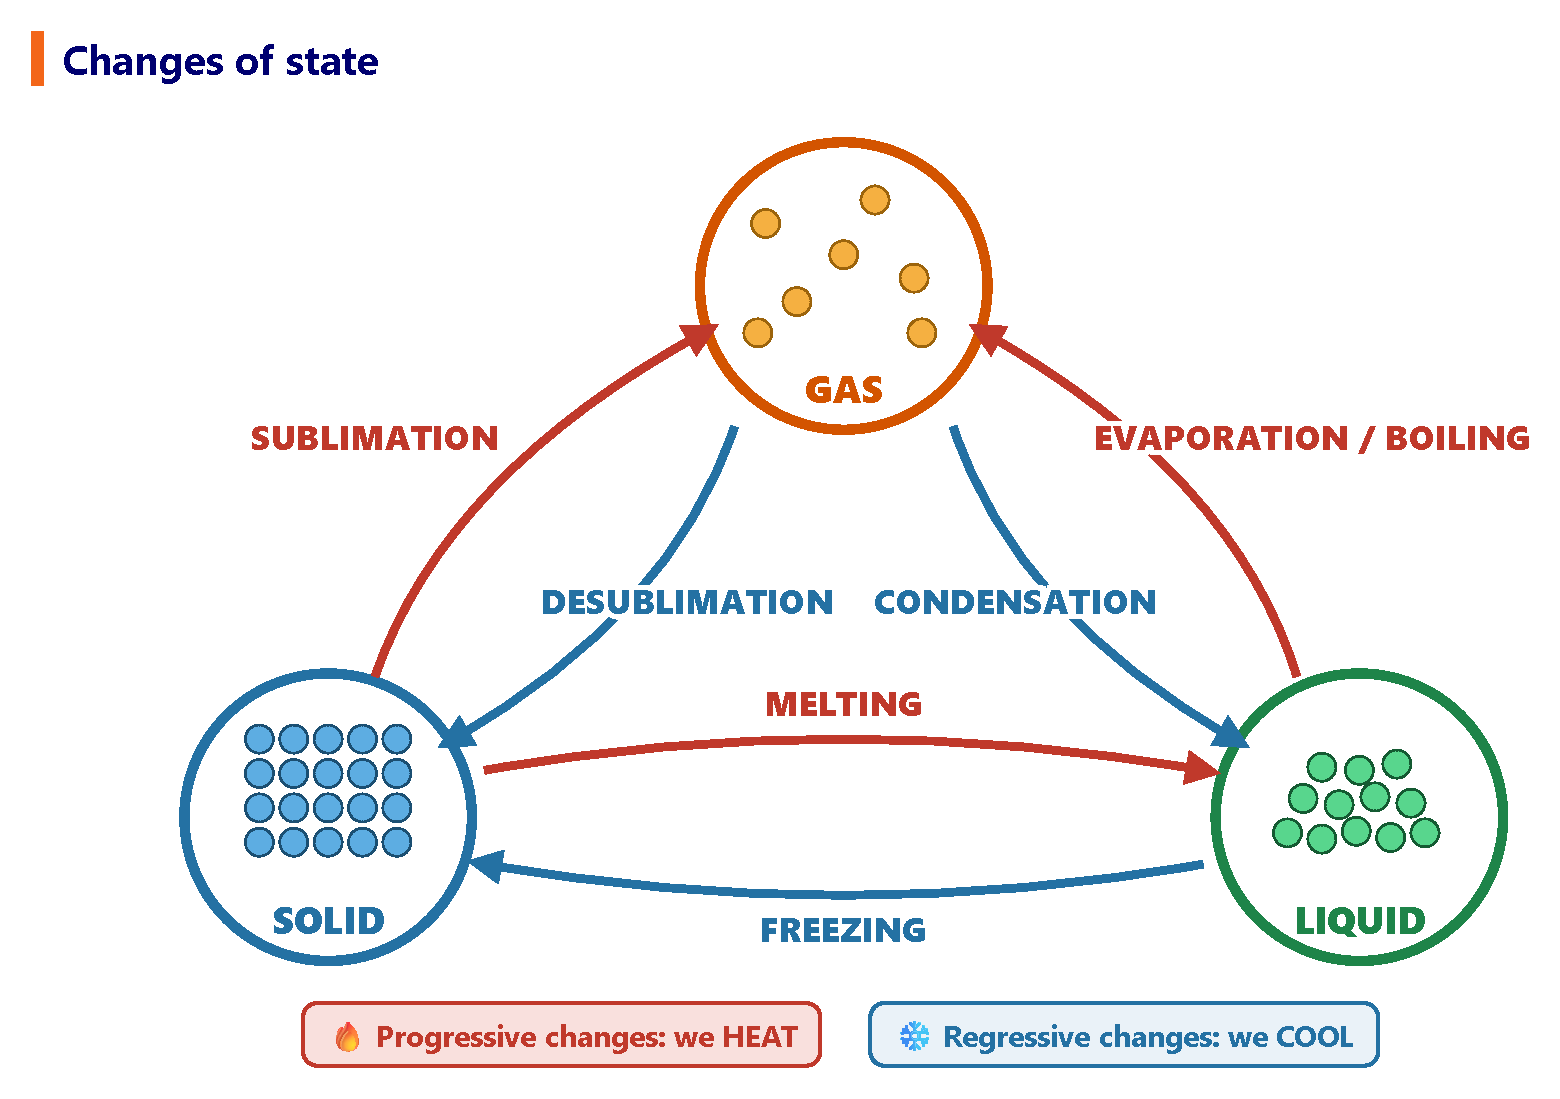
\includegraphics[width=0.95\textwidth]{FigurasSVG/Unit_2_State_of_Matter/pdf/changes_of_state.pdf}
    \caption{The six changes of state.}
    \label{fig:u2_changes_of_state}
\end{figure}

\begin{definition}[Melting point and boiling point]
    The \textbf{melting point} is the temperature at which a pure substance changes from solid to liquid; the \textbf{boiling point}, from liquid to gas. Both depend on pressure and are \textbf{characteristic properties}: each substance has its own values.
\end{definition}

\begin{table}[H]
    \centering
    \renewcommand{\arraystretch}{1.3}
    \begin{tabular}{lcc}
        \toprule
        \textbf{Substance} & \textbf{Melting point} & \textbf{Boiling point} \\
        \midrule
        Oxygen & \qty{-219}{\celsius} & \qty{-183}{\celsius} \\
        Alcohol & \qty{-114}{\celsius} & \qty{78}{\celsius} \\
        Mercury & \qty{-39}{\celsius} & \qty{357}{\celsius} \\
        Water & \qty{0}{\celsius} & \qty{100}{\celsius} \\
        Iron & \qty{1538}{\celsius} & \qty{2861}{\celsius} \\
        \bottomrule
    \end{tabular}
    \caption{Melting and boiling points of some substances.}
    \label{tab:u2_mp_bp}
\end{table}

\begin{impt}
    \textbf{Which state at room temperature?} Below its melting point a substance is \textbf{solid}; between its melting and boiling points it is \textbf{liquid}; above its boiling point it is a \textbf{gas}.
\end{impt}

\subsection{Heating curves and latent heat}

If we heat ice at a constant rate and write down its temperature every minute, we get a \negsubro{heating curve}:

\begin{figure}[H]
    \centering
    % [FIGURA ORIGINAL] \includegraphics[width=\textwidth]{Unit_2/heating_curve}
    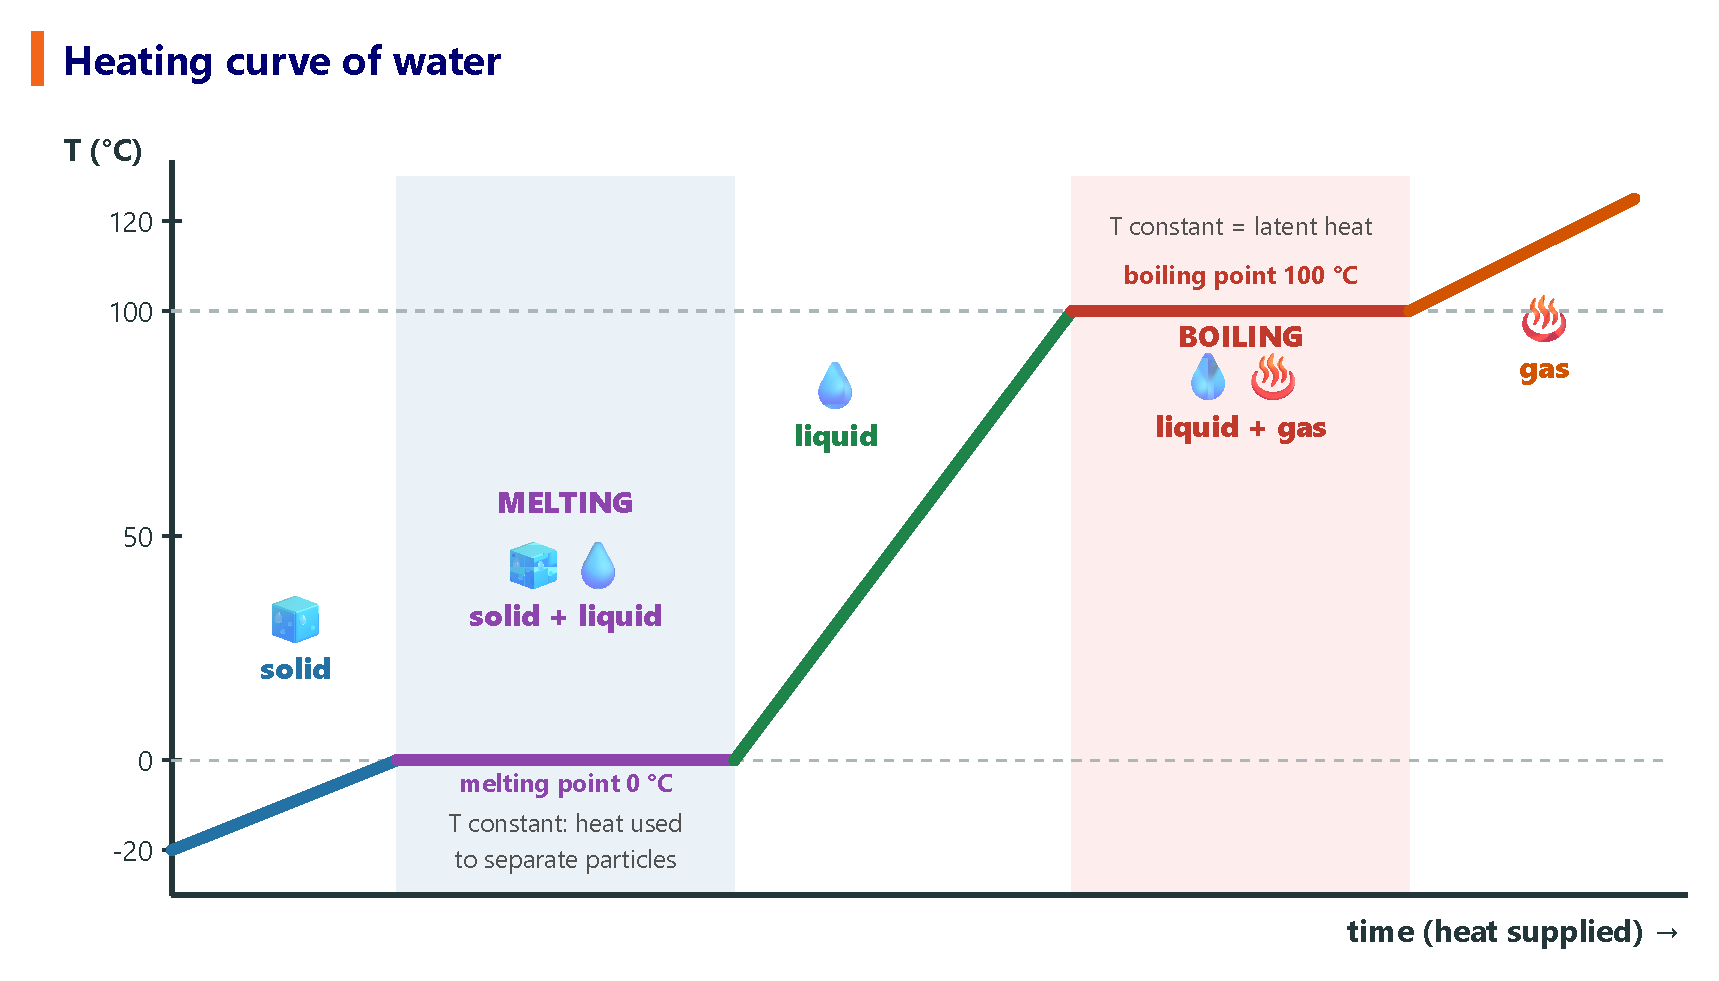
\includegraphics[width=\textwidth]{FigurasSVG/Unit_2_State_of_Matter/pdf/heating_curve.pdf}
    \caption{Heating curve of water: the temperature stays constant during each change of state.}
    \label{fig:u2_heating_curve}
\end{figure}

\begin{impt}
    While a pure substance is \textbf{changing state}, its \textbf{temperature does not change}, even if we keep heating it: the graph is flat (a ``plateau''). All the heat is used to separate the particles, not to make them move faster.
\end{impt}

\begin{definition}[Latent heat]
    The heat needed to change the state of \qty{1}{\kg} of a substance without changing its temperature. ``Latent'' means ``hidden'': we supply heat, but the thermometer does not show it.
\end{definition}

\subsection{Cooling curves}

If we do the opposite, and \textbf{cool} a substance at a constant rate while we write down its temperature every minute, we get a \negsubro{cooling curve}. It looks like the \textbf{mirror image} of the heating curve: the temperature goes \textbf{down}, and there are \textbf{plateaus} (flat parts) at the \textbf{same temperatures} as in the heating curve, while the gas condenses and while the liquid freezes.

\begin{figure}[H]
    \centering
    % [FIGURA ORIGINAL] \includegraphics[width=\textwidth]{Unit_2/cooling_curve}
    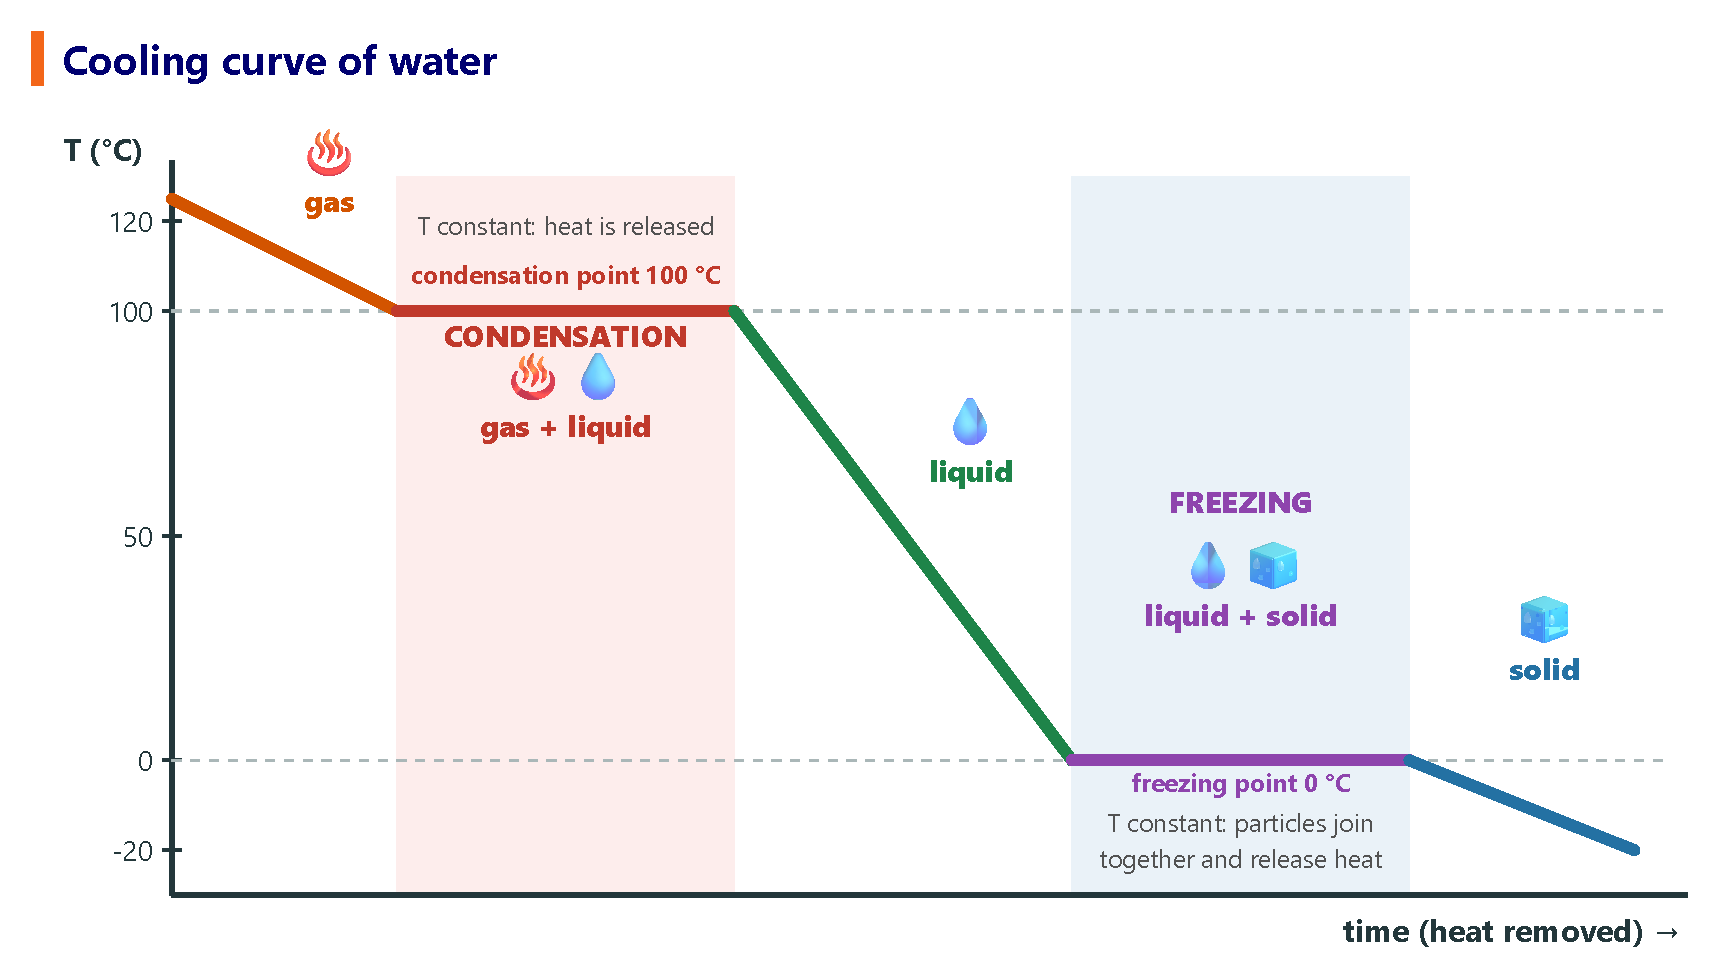
\includegraphics[width=\textwidth]{FigurasSVG/Unit_2_State_of_Matter/pdf/cooling_curve.pdf}
    \caption{Cooling curve of water: the temperature stays constant while the vapour condenses (\qty{100}{\celsius}) and while the liquid freezes (\qty{0}{\celsius}).}
    \label{fig:u2_cooling_curve}
\end{figure}

\begin{impt}
    \begin{itemize}
        \item In a cooling curve the substance \textbf{loses} heat. On the sloping parts its temperature goes down; on the flat parts it is \textbf{changing state} (condensation or freezing) and the temperature does \textbf{not} change.
        \item A pure substance \textbf{condenses} at the same temperature at which it \textbf{boils}, and it \textbf{freezes} at the same temperature at which it \textbf{melts}. For water: \qty{100}{\celsius} and \qty{0}{\celsius}.
    \end{itemize}
\end{impt}

\begin{example}
    \textbf{Reading the cooling curve of water.} We start with water vapour at \qty{125}{\celsius} and take heat away from it:
    \begin{enumerate}[label=\numberballmDarkTeal]
        \item From \qty{125}{\celsius} to \qty{100}{\celsius}: there is only \textbf{gas}, and its temperature goes down.
        \item At \qty{100}{\celsius}: the line is flat. The vapour is \textbf{condensing}: \textbf{gas and liquid} are together and the temperature does not change.
        \item From \qty{100}{\celsius} to \qty{0}{\celsius}: there is only \textbf{liquid}, and it gets colder.
        \item At \qty{0}{\celsius}: the line is flat again. The water is \textbf{freezing}: \textbf{liquid and solid} are together.
        \item Below \qty{0}{\celsius}: there is only \textbf{solid} (ice), and it keeps getting colder.
    \end{enumerate}
\end{example}

\begin{example}
    \textbf{Cooling curve of paraffin wax.} Liquid wax at \qty{80}{\celsius} is left to cool, and its temperature is written down every minute:
    \begin{center}
        \renewcommand{\arraystretch}{1.3}
        % --- tabla antigua ---
        % \begin{tabular}{l|cccccccc}
            % \textbf{Time (min)} & 0 & 1 & 2 & 3 & 4 & 5 & 6 & 7 \\
            % \hline
            % \textbf{T (\unit{\celsius})} & 80 & 70 & 60 & 55 & 55 & 55 & 45 & 35 \\
        % \end{tabular}
        % --- tabla nueva ---
        \begin{tabular}{@{}lcccccccc@{}}
            \toprule
            \textbf{Time (min)} & \textbf{0} & \textbf{1} & \textbf{2} & \textbf{3} & \textbf{4} & \textbf{5} & \textbf{6} & \textbf{7} \\
            \midrule
            \textbf{T (\unit{\celsius})} & 80 & 70 & 60 & 55 & 55 & 55 & 45 & 35 \\
            \bottomrule
        \end{tabular}
    \end{center}
    From minute 3 to minute 5 the temperature stays at \qty{55}{\celsius}: that is the plateau. So the wax \textbf{freezes} (and also melts) at \textcolor{red}{\qty{55}{\celsius}}. Before minute 3 the wax is liquid, between minutes 3 and 5 liquid and solid wax are together, and after minute 5 it is solid.
\end{example}

\begin{example}
    \textbf{Worked example: reading a heating curve step by step.} In the laboratory we heat an unknown pure substance at a constant rate, starting at \qty{-130}{\celsius}, and write down its temperature every minute:
    \begin{center}
        \renewcommand{\arraystretch}{1.3}
        \begin{tabular}{@{}lcccccccccccc@{}}
            \toprule
            \textbf{Time (min)} & \textbf{0} & \textbf{1} & \textbf{2} & \textbf{3} & \textbf{4} & \textbf{5} & \textbf{6} & \textbf{7} & \textbf{8} & \textbf{9} & \textbf{10} & \textbf{11} \\
            \midrule
            \textbf{T (\unit{\celsius})} & \(-130\) & \(-114\) & \(-114\) & \(-114\) & \(-50\) & 14 & 78 & 78 & 78 & 78 & 90 & 102 \\
            \bottomrule
        \end{tabular}
    \end{center}
    We want to know: \textbf{a)} its melting point and boiling point; \textbf{b)} its physical state in each part of the experiment; \textbf{c)} which substance it is.
    \begin{enumerate}[label=\numberballmDarkTeal]
        \item \textbf{Draw the graph.} Put the \textbf{time} on the horizontal axis and the \textbf{temperature} on the vertical axis, choose a scale that fits all the values (from \qty{-140}{\celsius} to \qty{120}{\celsius}), plot each pair of values as a point and join the points with straight lines (Figure~\ref{fig:u2_heating_curve_example}).
        \item \textbf{Look for the plateaus.} We look for the parts of the table where the temperature \textbf{does not change}, although we keep heating:
        \begin{itemize}
            \item from minute 1 to minute 3 the temperature stays at \qty{-114}{\celsius};
            \item from minute 6 to minute 9 the temperature stays at \qty{78}{\celsius}.
        \end{itemize}
        \item \textbf{Name the changes of state.} We are \textbf{heating}, so the first plateau (the lower temperature) is \textbf{melting} and the second one (the higher temperature) is \textbf{boiling}. Therefore:
        \[
            \text{melting point} = \textcolor{red}{\qty{-114}{\celsius}} \qquad \text{boiling point} = \textcolor{red}{\qty{78}{\celsius}}
        \]
        \item \textbf{Write the state in each part.} Below the melting point the substance is solid; on a plateau two states are together; between the two plateaus it is liquid; above the boiling point it is gas:
        \begin{itemize}
            \item from 0 to 1 min: \textbf{solid}, and its temperature goes up;
            \item from 1 to 3 min: \textbf{solid + liquid} (it is melting), constant temperature;
            \item from 3 to 6 min: \textbf{liquid}, and its temperature goes up;
            \item from 6 to 9 min: \textbf{liquid + gas} (it is boiling), constant temperature;
            \item from 9 to 11 min: \textbf{gas}, and its temperature goes up.
        \end{itemize}
        \item \textbf{Identify the substance.} Melting and boiling points are \textbf{characteristic properties}, so we compare our values with Table~\ref{tab:u2_mp_bp}: the substance that melts at \qty{-114}{\celsius} and boils at \qty{78}{\celsius} is \textcolor{red}{\textbf{alcohol}}.
        \item \textbf{Check the answer.} At room temperature (\qty{20}{\celsius}) our substance would be between its melting and boiling points, so it would be a \textbf{liquid}. That is right: alcohol is a liquid at room temperature.
    \end{enumerate}
\end{example}

\begin{figure}[H]
    \centering
    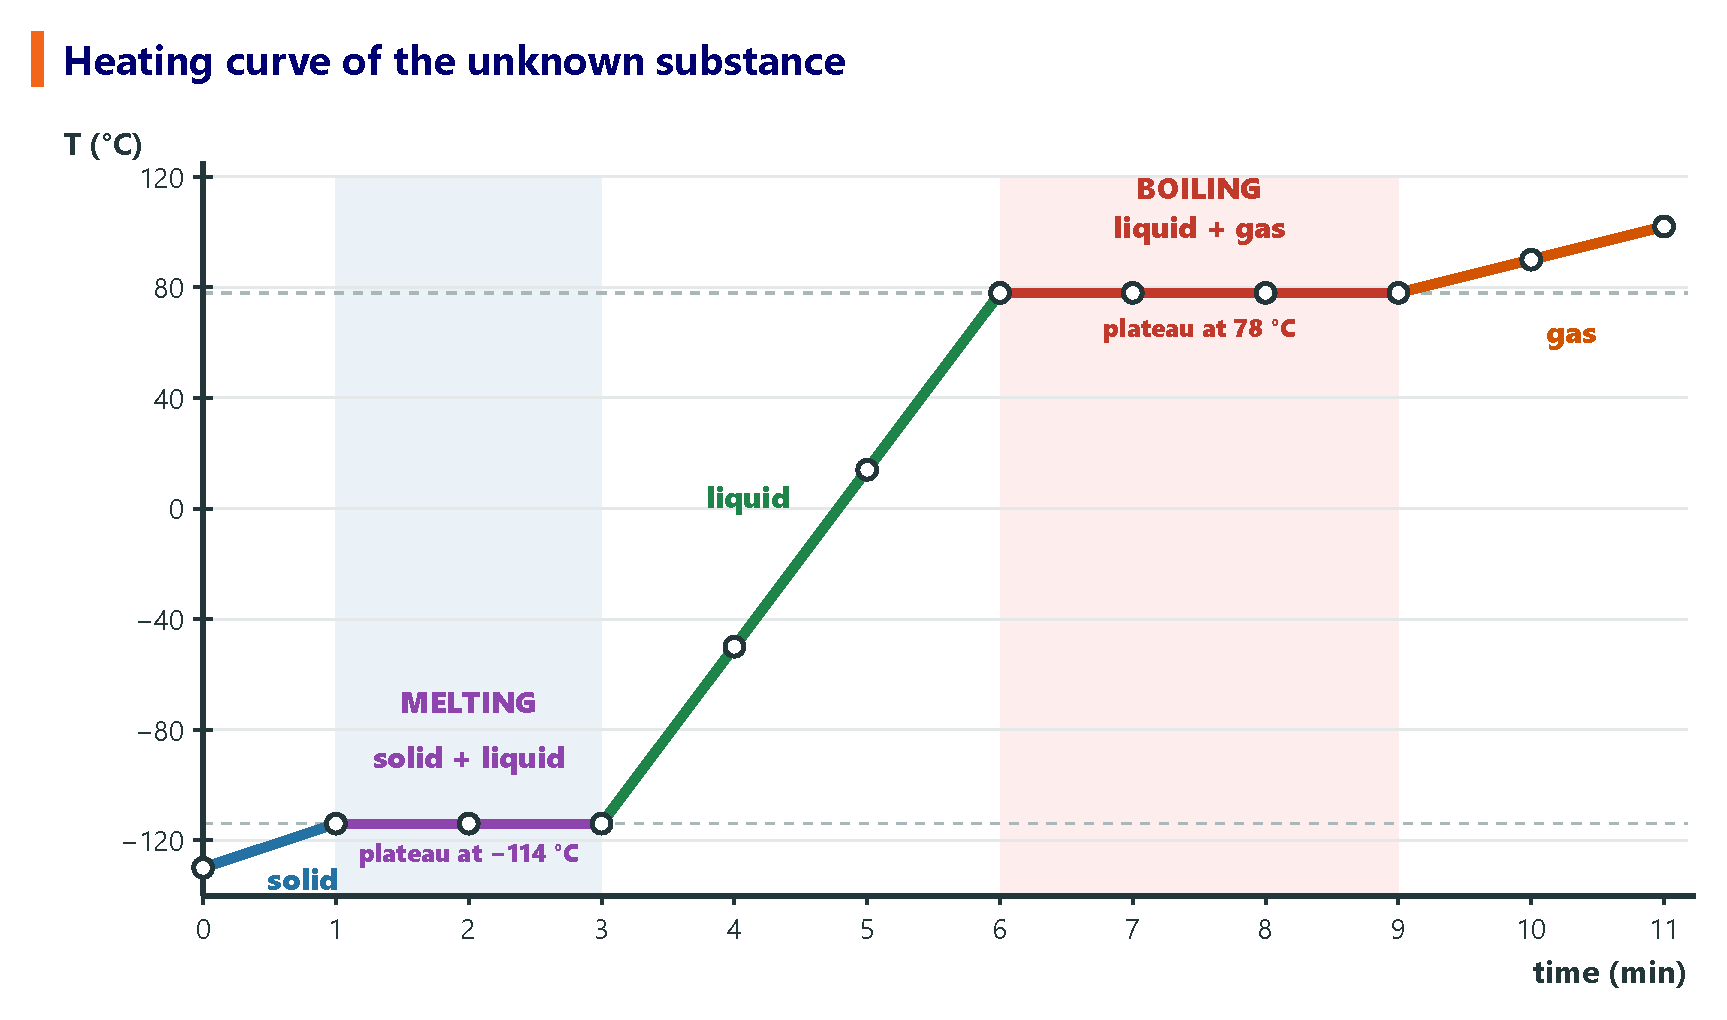
\includegraphics[width=\textwidth]{FigurasSVG/Unit_2_State_of_Matter/pdf/heating_curve_example.pdf}
    \caption{Heating curve drawn from the data of the worked example: the plateaus at \qty{-114}{\celsius} and \qty{78}{\celsius} are the melting and boiling points of alcohol.}
    \label{fig:u2_heating_curve_example}
\end{figure}

\begin{exercise}
    A sample of a pure substance is heated at a constant rate, and its temperature is recorded every minute: \qty{-10}{\celsius}, \qty{0}{\celsius}, \qty{0}{\celsius}, \qty{0}{\celsius}, \qty{20}{\celsius}, \qty{40}{\celsius} (at \(t = 0, 1, 2, 3, 4, 5\) min).
    \begin{enumerate}[label=\letraminuscula]
        \item What is the melting point of the substance?
        \item In which minutes is the substance changing state? Which states coexist?
        \item Could this substance be water? Justify your answer.
    \end{enumerate}
    \begin{solu}
        \begin{enumerate}[label=\alph*)]
            \item The temperature stays constant at \qty{0}{\celsius}, so the melting point is \qty{0}{\celsius}.
            \item Between \(t = 1\) and \(t = 3\) min; \textbf{solid and liquid} coexist.
            \item \textbf{Yes}, it could be water: its melting point (\qty{0}{\celsius}) matches the melting point of water at \qty{1}{\atmospher}.
        \end{enumerate}
    \end{solu}
\end{exercise}

\begin{exercise}
    Molten candle wax cools at room temperature, and its temperature is recorded every 2 minutes: \qty{80}{\celsius}, \qty{60}{\celsius}, \qty{45}{\celsius}, \qty{45}{\celsius}, \qty{45}{\celsius}, \qty{45}{\celsius}, \qty{30}{\celsius}, \qty{22}{\celsius} (at \(t = 0, 2, 4, 6, 8, 10, 12, 14\) min).
    \begin{enumerate}[label=\letraminuscula]
        \item Draw the cooling curve (temperature on the vertical axis, time on the horizontal axis).
        \item What is the freezing point of the wax?
        \item During which minutes is the wax changing state, and what states coexist?
    \end{enumerate}
    \begin{solu}
        \begin{enumerate}[label=\alph*)]
            \item The curve falls from \qty{80}{\celsius} to \qty{45}{\celsius}, stays flat at \qty{45}{\celsius} for several minutes, and then falls again to \qty{22}{\celsius}.
            \item \qty{45}{\celsius}.
            \item Between \(t = 4\) and \(t = 10\) min; \textbf{liquid and solid} wax coexist.
        \end{enumerate}
    \end{solu}
\end{exercise}

\begin{exercise}
    A student says: ``If I turn the gas on the stove up as high as possible, the water in the pan will boil at a much higher temperature, so my pasta will cook faster.'' Is the student right? Use the idea of latent heat.
    \begin{solu}
        The student is \textbf{wrong}. Once water reaches its boiling point (\qty{100}{\celsius} at \qty{1}{\atmospher}), its temperature stays constant however much heat we supply. More heat only makes the water boil \textbf{more vigorously}: the extra heat is used as latent heat to turn more liquid into gas, not to raise the temperature.
    \end{solu}
\end{exercise}

\subsection{Evaporation vs.\ boiling}

\begin{figure}[H]
    \centering
    % [FIGURA ORIGINAL] \includegraphics[width=\textwidth]{Unit_2/evaporation_boiling}
    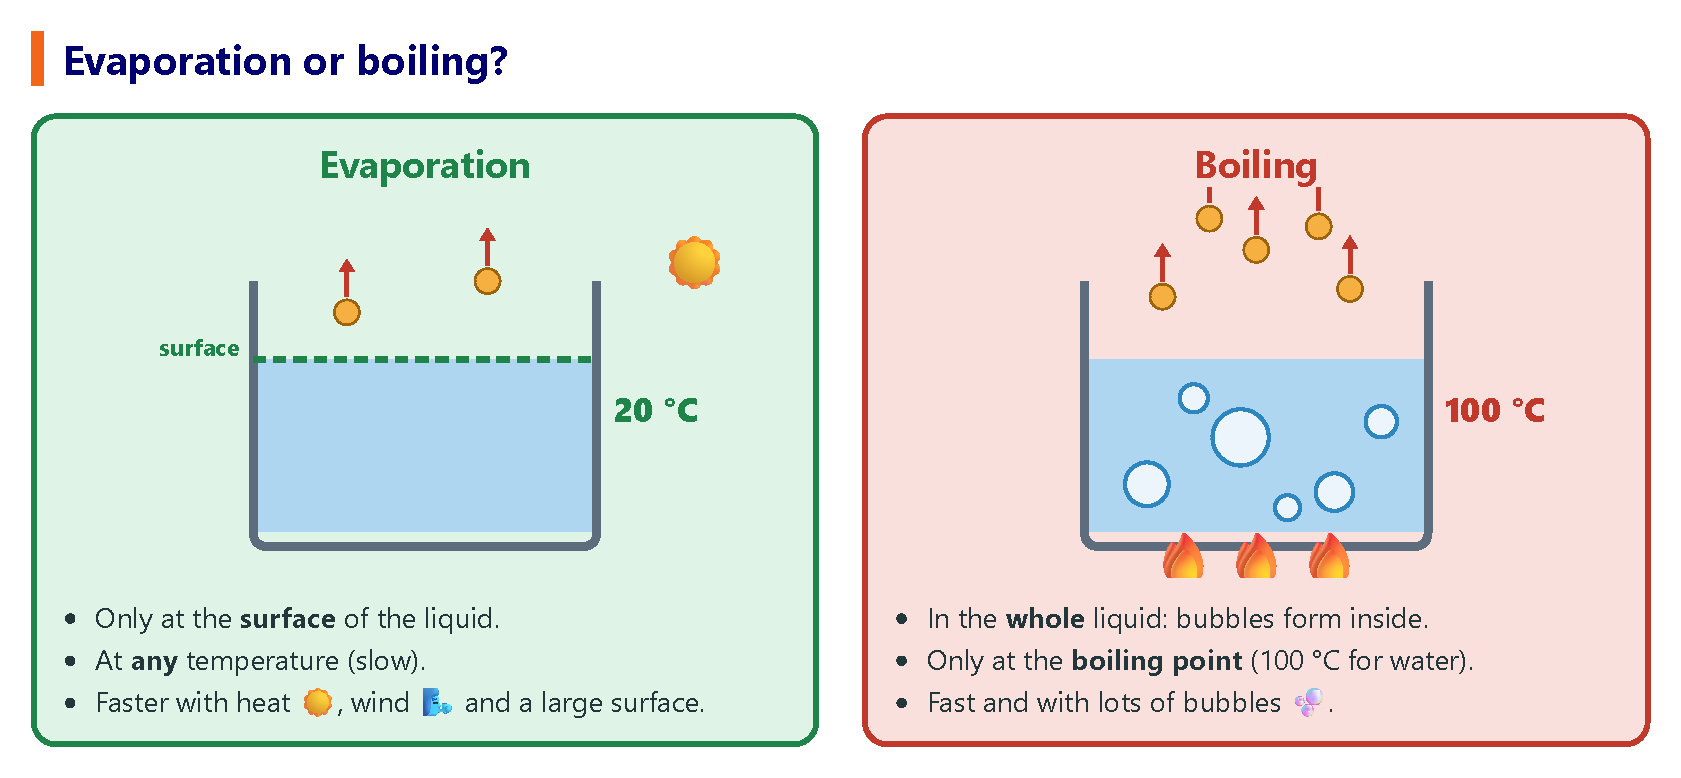
\includegraphics[width=\textwidth]{FigurasSVG/Unit_2_State_of_Matter/pdf/evaporation_boiling.pdf}
    \caption{Two ways of turning a liquid into a gas.}
    \label{fig:u2_evaporation_boiling}
\end{figure}

\begin{exercise}
    Classify each situation as evaporation or boiling, and justify your answer.
    \begin{enumerate}[label=\letraminuscula]
        \item Wet clothes hung out on a washing line dry after a few hours.
        \item Water in a saucepan bubbles vigorously on the stove at \qty{100}{\celsius}.
        \item A puddle on the pavement slowly disappears over a warm afternoon.
        \item Milk in a pan rises and bubbles all the way through just before it ``boils over''.
    \end{enumerate}
    \begin{solu}
        \begin{enumerate}[label=\alph*)]
            \item \textbf{Evaporation}: at the surface of the wet fabric, well below \qty{100}{\celsius}.
            \item \textbf{Boiling}: bubbles form throughout the whole liquid, at its boiling point.
            \item \textbf{Evaporation}: only at the surface of the puddle, at outdoor temperature.
            \item \textbf{Boiling}: the whole mass of milk is affected, not just the surface.
        \end{enumerate}
    \end{solu}
\end{exercise}

\begin{exercise}
    Explain why washing dries faster on a windy, sunny day than on a still, cloudy day, and why spreading the clothes out also makes them dry faster.
    \begin{solu}
        Drying clothes is \textbf{evaporation}. The Sun raises the temperature, so the water particles have more energy to escape; the wind carries the vapour away as soon as it forms. Spreading the clothes out increases the \textbf{surface area}, and evaporation is faster with a larger surface.
    \end{solu}
\end{exercise}

\subsection{Sublimation and desublimation}

Some substances, such as iodine or solid carbon dioxide (``dry ice''), change directly between solid and gas, \textbf{without} becoming a liquid:

\begin{itemize}
    \item \negsubro{Sublimation}: solid \(\to\) gas.
    \item \negsubro{Desublimation}: gas \(\to\) solid (for example, frost on a cold morning).
\end{itemize}

\begin{impt}
    Changes that happen when we \textbf{heat} (melting, evaporation, sublimation) are \negsubro{progressive}. Changes that happen when we \textbf{cool} (freezing, condensation, desublimation) are \negsubro{regressive}.
\end{impt}

\begin{didyouknow}
    The ``smoke'' that comes out of dry ice at concerts is not carbon dioxide gas, which is invisible! The very cold gas cools the air around it, and the water vapour in the air condenses into tiny drops: a man-made fog.
\end{didyouknow}

\begin{exercise}
    Blocks of solid carbon dioxide (``dry ice'') are often used to create a fog effect on stage.
    \begin{enumerate}[label=\letraminuscula]
        \item What change of state takes place as the dry ice ``disappears'', and is it progressive or regressive?
        \item Unlike an ice cube, dry ice never leaves a puddle of liquid behind. Why?
    \end{enumerate}
    \begin{solu}
        \begin{enumerate}[label=\alph*)]
            \item \textbf{Sublimation} (solid \(\to\) gas), a \textbf{progressive} change.
            \item At atmospheric pressure, solid carbon dioxide passes directly from solid to gas, without going through the liquid state.
        \end{enumerate}
    \end{solu}
\end{exercise}

\begin{exercise}
    Mothballs slowly get smaller over the weeks, even though they are never heated, and eventually disappear without leaving any liquid. Explain what is happening and name the change of state.
    \begin{solu}
        The mothball is \textbf{sublimating}: its particles pass directly from solid to gas (releasing a smell that repels insects), without ever becoming a liquid. This can happen slowly at room temperature.
    \end{solu}
\end{exercise}

\subsection{The effect of pressure on boiling}

\begin{figure}[H]
    \centering
    % [FIGURA ORIGINAL] \includegraphics[width=\textwidth]{Unit_2/pressure_boiling}
    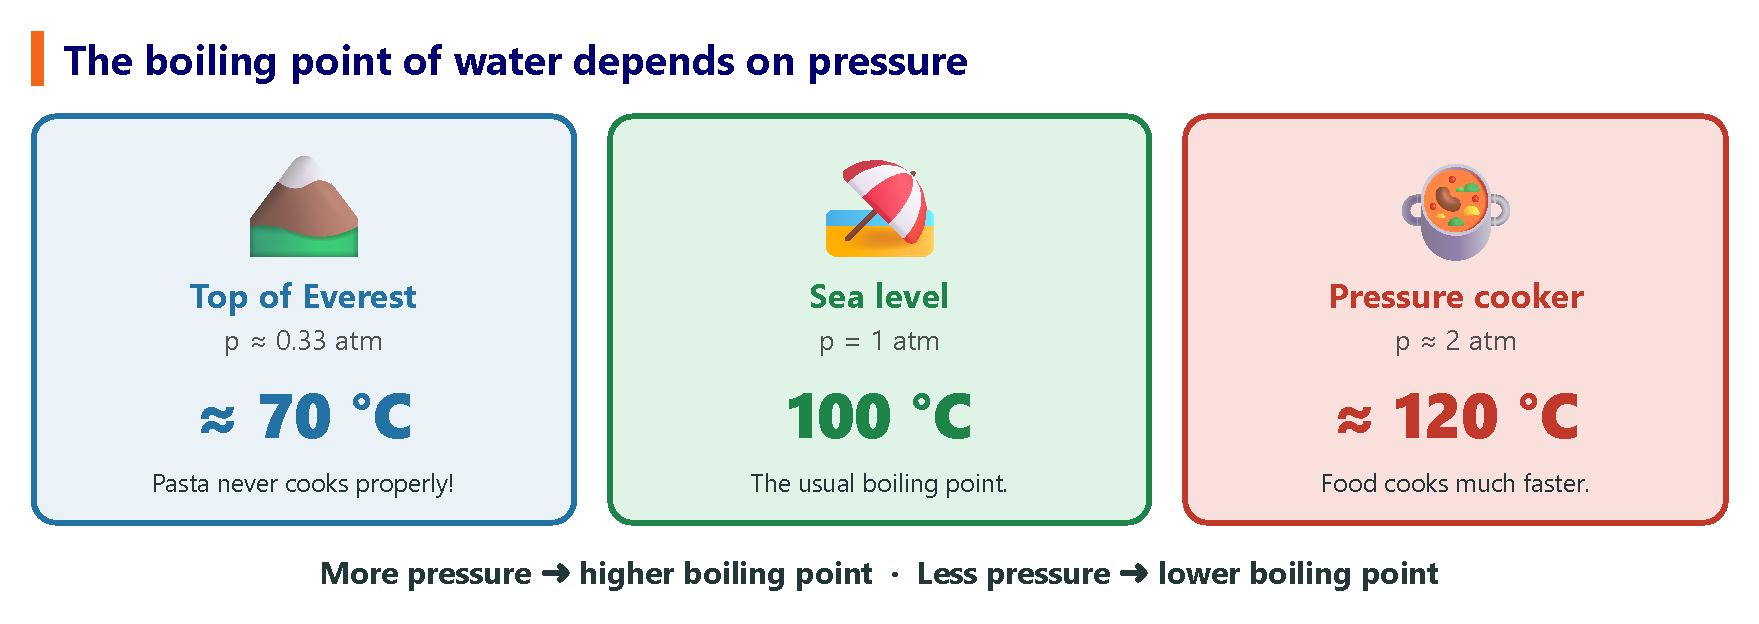
\includegraphics[width=\textwidth]{FigurasSVG/Unit_2_State_of_Matter/pdf/pressure_boiling.pdf}
    \caption{The boiling point of water changes with pressure.}
    \label{fig:u2_pressure_boiling}
\end{figure}

\begin{exercise}
    Use the table of melting and boiling points at the beginning of this section to indicate the physical state of oxygen, alcohol, water and iron at \qty{20}{\celsius} and \qty{1}{\atmospher}.
    \begin{solu}
        Oxygen: \textbf{gas} (\(20 > -183\)). \\
        Alcohol: \textbf{liquid} (\(-114 < 20 < 78\)). \\
        Water: \textbf{liquid} (\(0 < 20 < 100\)). \\
        Iron: \textbf{solid} (\(20 < 1538\)).
    \end{solu}
\end{exercise}

\begin{exercise}
    A liquid is cooled in a freezer. Its temperature is recorded every \qty{10}{\minute}: \qty{20}{\celsius}, \qty{6}{\celsius}, \qty{-8}{\celsius}, \qty{-8}{\celsius}, \qty{-8}{\celsius}, \qty{-22}{\celsius} (at \(t = 0, 10, 20, 30, 40, 50\) min).
    \begin{enumerate}[label=\letraminuscula]
        \item What is the freezing point of this substance?
        \item Can the substance be water? Why?
    \end{enumerate}
    \begin{solu}
        \begin{enumerate}[label=\alph*)]
            \item The temperature stays constant at \qty{-8}{\celsius} between \(t = 20\) and \(t = 40\) min, so the freezing point is \qty{-8}{\celsius}.
            \item \textbf{No}, because water freezes at \qty{0}{\celsius}.
        \end{enumerate}
    \end{solu}
\end{exercise}

\begin{exercise}
    A puddle dries up on a sunny day; the bathroom mirror steams up during a hot shower; frost forms on leaves on a very cold, clear night; an ice lolly drips in the sun. Identify the change of state in each case, and say whether it is progressive or regressive.
    \begin{solu}
        Puddle: \textbf{evaporation}, progressive. \\
        Mirror: \textbf{condensation}, regressive. \\
        Frost: \textbf{desublimation}, regressive. \\
        Ice lolly: \textbf{melting}, progressive.
    \end{solu}
\end{exercise}

%----------------------------------------------------------------------------------------

\section{States of water and meteorology}

Water is the only substance that we find naturally in the three states on Earth. Its changes of state create the weather we see every day:

\begin{figure}[H]
    \centering
    % [FIGURA ORIGINAL] \includegraphics[width=\textwidth]{Unit_2/weather_phenomena}
    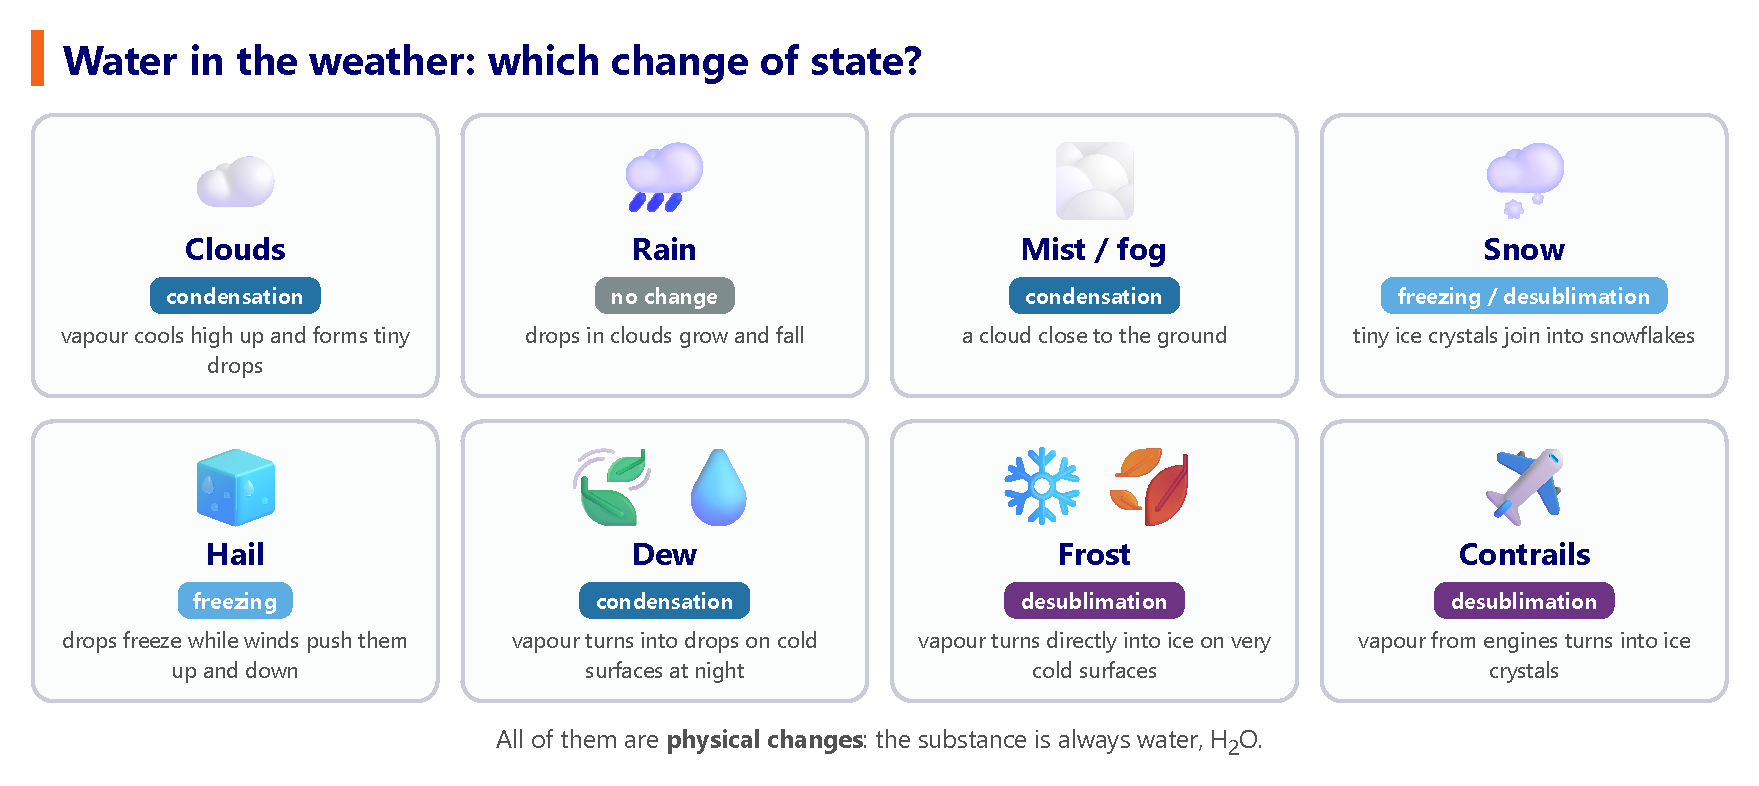
\includegraphics[width=\textwidth]{FigurasSVG/Unit_2_State_of_Matter/pdf/weather_phenomena.pdf}
    \caption{Weather phenomena and the change of state behind each one.}
    \label{fig:u2_weather_phenomena}
\end{figure}

\begin{exercise}
    Name the physical state in which water is found in: clouds, air, hail, snow, dew, frost.
    \begin{solu}
        Clouds: liquid (drops) or solid (ice crystals). Air: gas (water vapour). Hail: solid. Snow: solid. Dew: liquid. Frost: solid.
    \end{solu}
\end{exercise}

\begin{exercise}
    When we breathe out on a cold winter day, we can see a small cloud coming out of our mouths, but this does not happen indoors. Why?
    \begin{solu}
        Our breath contains warm water vapour. Outdoors, in cold air, it cools very quickly and \textbf{condenses} into tiny visible drops. Indoors, the air is warmer, so the vapour does not condense and stays as an invisible gas.
    \end{solu}
\end{exercise}

\begin{exercise}
    Match each weather phenomenon with the change of state involved, and say whether it is progressive or regressive: (1) dew, (2) frost, (3) mist, (4) hail.
    \begin{enumerate}[label=\letraminuscula]
        \item[A] Condensation of water vapour into liquid drops.
        \item[B] Desublimation of water vapour directly into a solid.
        \item[C] Evaporation followed by condensation close to the ground.
        \item[D] Freezing of liquid drops carried up and down inside a cloud.
    \end{enumerate}
    \begin{solu}
        (1) Dew \(\to\) A, condensation, regressive. \\
        (2) Frost \(\to\) B, desublimation, regressive. \\
        (3) Mist \(\to\) C, evaporation (progressive) followed by condensation (regressive); the visible mist itself is formed by condensation. \\
        (4) Hail \(\to\) D, freezing, regressive.
    \end{solu}
\end{exercise}

\subsection{The water cycle}

Water is always moving between the sea, the air and the land, and changing state on the way. This is the \negsubro{water cycle}, and its engine is the \textbf{Sun}.

\begin{figure}[H]
    \centering
    % [FIGURA ORIGINAL] \includegraphics[width=\textwidth]{Unit_2/water_cycle}
    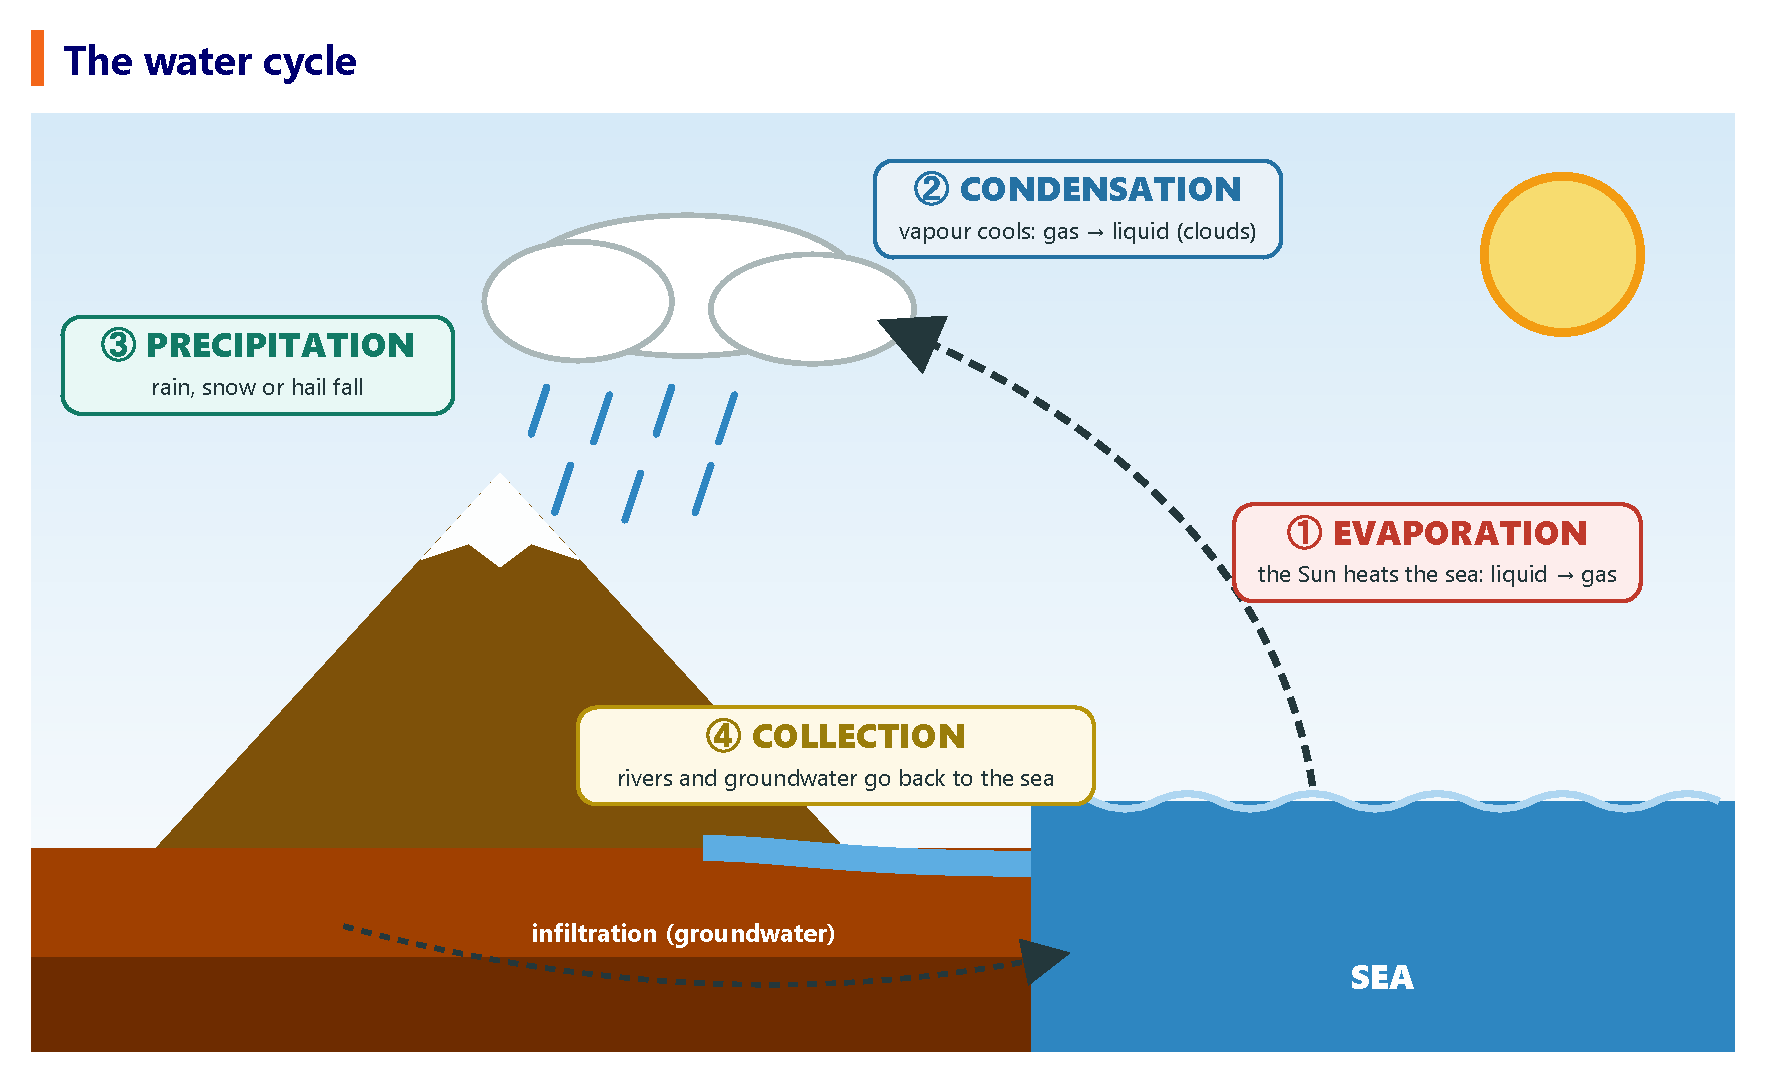
\includegraphics[width=\textwidth]{FigurasSVG/Unit_2_State_of_Matter/pdf/water_cycle.pdf}
    \caption{The four stages of the water cycle.}
    \label{fig:u2_water_cycle}
\end{figure}

\begin{impt}
    The water cycle involves \textbf{only physical changes}: the substance is always water, \ch{H2O}, whatever state it is in.
\end{impt}

\begin{didyouknow}
    The water you drink today is the same water the dinosaurs drank millions of years ago! The amount of water on Earth hardly changes: it just keeps going round and round the water cycle.
\end{didyouknow}

\begin{exercise}
    Order these stages of the water cycle correctly, and name the change of state involved in each one: (1) clouds form over the sea; (2) rain falls over the mountains; (3) the Sun heats the surface of the ocean; (4) rivers carry the water back to the sea.
    \begin{solu}
        Correct order: 3, 1, 2, 4. \\
        (3) Water turns into vapour: \textbf{evaporation}. \\
        (1) Water vapour cools down and forms tiny droplets: \textbf{condensation}. \\
        (2) The droplets grow and fall: \textbf{precipitation} (no change of state). \\
        (4) Liquid water flows back to the sea (no change of state).
    \end{solu}
\end{exercise}

\begin{exercise}
    Explain why the water cycle is said to involve ``only physical changes'', and why it could not continue without the Sun.
    \begin{solu}
        Although water changes state many times, it is always the \textbf{same substance}, \ch{H2O}: no new substances are formed. The Sun supplies the energy needed for \textbf{evaporation}; without it, no water vapour would form, there would be no clouds and no precipitation.
    \end{solu}
\end{exercise}

\begin{exercise}
    ``Most of the water that falls as rain over a mountain range originally evaporated from the ocean, sometimes hundreds of kilometres away.''
    \begin{enumerate}[label=\letraminuscula]
        \item Describe, step by step, how a water particle could travel from the ocean to a raindrop falling on a mountain.
        \item Once the rain falls on the mountain, name two possible paths the water can then follow.
    \end{enumerate}
    \begin{solu}
        \begin{enumerate}[label=\alph*)]
            \item The Sun heats the ocean and the water \textbf{evaporates}. Winds carry the vapour inland; as it rises over the mountains it cools and \textbf{condenses} into tiny droplets (a cloud). When the droplets are big enough they fall as \textbf{rain}.
            \item It can flow over the surface (streams and rivers) back to the sea, or \textbf{infiltrate} into the ground and become groundwater.
        \end{enumerate}
    \end{solu}
\end{exercise}

%----------------------------------------------------------------------------------------

\section*{Summary}

\begin{itemize}
    \item \textbf{States of matter}: solids (fixed shape and volume), liquids (fixed volume, variable shape), gases (variable shape and volume).
    \item \textbf{Kinetic theory}: matter is made of particles that are always moving; the faster they move, the higher the temperature. It explains diffusion, compressibility, thermal expansion and gas pressure.
    \item \textbf{Gas pressure}: caused by gas particles hitting the walls of the container.
    \item \textbf{Gas laws} (temperature always in kelvin, \(T(\unit{\K}) = T(\unit{\celsius}) + 273\)): Boyle-Mariotte (\(p \cdot V = \text{const.}\)); Gay-Lussac (\(p/T = \text{const.}\)); Charles (\(V/T = \text{const.}\)); general gas law (\(p \cdot V / T = \text{const.}\)).
    \item \textbf{Changes of state}: progressive (melting, evaporation/boiling, sublimation) and regressive (freezing, condensation, desublimation). The temperature stays constant during a change of state, because the heat is used as \textbf{latent heat}.
    \item \textbf{Evaporation} happens at the surface, at any temperature; \textbf{boiling} happens in the whole liquid, at the boiling point.
    \item \textbf{Pressure and boiling point}: more pressure \(\to\) higher boiling point (pressure cooker); less pressure \(\to\) lower boiling point (mountains).
    \item \textbf{Meteorology and the water cycle}: clouds, mist and dew form by condensation; frost and contrails by desublimation; hail by freezing. The Sun drives the water cycle: evaporation, condensation, precipitation and collection.
\end{itemize}

\section{Vocabulary}

\begin{vocabulary}[Kinetic theory]
    The theory explaining that matter is made up of moving particles, whose behaviour depends on their state. \newline
    \textbf{Translation to Spanish}: Teoría cinética
\end{vocabulary}

\begin{vocabulary}[Melting]
    Change of state from solid to liquid. \newline
    \textbf{Translation to Spanish}: Fusión
\end{vocabulary}

\begin{vocabulary}[Freezing]
    Change of state from liquid to solid. \newline
    \textbf{Translation to Spanish}: Solidificación
\end{vocabulary}

\begin{vocabulary}[Evaporation]
    Change of state from liquid to gas, occurring at the surface of the liquid. \newline
    \textbf{Translation to Spanish}: Evaporación
\end{vocabulary}

\begin{vocabulary}[Boiling]
    Change of state from liquid to gas, occurring throughout the liquid at the boiling point. \newline
    \textbf{Translation to Spanish}: Ebullición
\end{vocabulary}

\begin{vocabulary}[Condensation]
    Change of state from gas to liquid. \newline
    \textbf{Translation to Spanish}: Condensación
\end{vocabulary}

\begin{vocabulary}[Sublimation]
    Change of state directly from solid to gas. \newline
    \textbf{Translation to Spanish}: Sublimación
\end{vocabulary}

\begin{vocabulary}[Desublimation]
    Change of state directly from gas to solid. \newline
    \textbf{Translation to Spanish}: Sublimación inversa
\end{vocabulary}

\begin{vocabulary}[Melting point]
    Temperature at which a substance changes from solid to liquid. \newline
    \textbf{Translation to Spanish}: Punto de fusión
\end{vocabulary}

\begin{vocabulary}[Boiling point]
    Temperature at which a substance changes from liquid to gas. \newline
    \textbf{Translation to Spanish}: Punto de ebullición
\end{vocabulary}

\begin{vocabulary}[Pressure]
    The force exerted by the particles of a gas as they hit the walls of the container. \newline
    \textbf{Translation to Spanish}: Presión
\end{vocabulary}

\begin{vocabulary}[Diffusion]
    The process by which the particles of a gas or liquid spread out and mix, until they are evenly distributed. \newline
    \textbf{Translation to Spanish}: Difusión
\end{vocabulary}

\begin{vocabulary}[General gas law]
    The equation $p \cdot V / T = \text{constant}$, which relates pressure, volume and temperature when none of the three is fixed. \newline
    \textbf{Translation to Spanish}: Ley general de los gases
\end{vocabulary}

\begin{vocabulary}[Heating curve]
    A graph showing how the temperature of a substance changes over time as it is heated at a constant rate, with flat sections during changes of state. \newline
    \textbf{Translation to Spanish}: Curva de calentamiento
\end{vocabulary}

\begin{vocabulary}[Latent heat]
    The heat needed to change the state of a substance at constant temperature. \newline
    \textbf{Translation to Spanish}: Calor latente
\end{vocabulary}

\begin{vocabulary}[Absolute zero]
    The lowest possible temperature, 0 K (\qty{-273}{\celsius}), at which particles stop moving. \newline
    \textbf{Translation to Spanish}: Cero absoluto
\end{vocabulary}

\begin{vocabulary}[Progressive change]
    A change of state that happens when a substance is heated (melting, evaporation, sublimation). \newline
    \textbf{Translation to Spanish}: Cambio progresivo
\end{vocabulary}

\begin{vocabulary}[Regressive change]
    A change of state that happens when a substance is cooled (freezing, condensation, desublimation). \newline
    \textbf{Translation to Spanish}: Cambio regresivo
\end{vocabulary}

\begin{vocabulary}[Water cycle]
    The continuous movement of water between the oceans, the atmosphere and the land, through evaporation, condensation, precipitation and collection. \newline
    \textbf{Translation to Spanish}: Ciclo del agua
\end{vocabulary}



%------------------------------------------------


    \chapterimage{images/portada_cabeceras/cabecera_Unit3}
    \chapter{Diversity of Matter}
    % Saberes básicos (LOMLOE) asociados a esta unidad
%
% Bloque B. La materia
%   - Teoría cinético-molecular: aplicación a observaciones sobre la materia
%     explicando la formación de mezclas y disoluciones — la unidad clasifica
%     mezclas homogéneas/heterogéneas, disoluciones, coloides y emulsiones a
%     partir del tamaño de partícula.
%   - Experimentos relacionados con los sistemas materiales: conocimiento y
%     descripción de sus propiedades, su composición y su clasificación —
%     se distinguen sustancias puras de mezclas y se caracteriza cada tipo
%     mediante propiedades como el punto de fusión o la concentración.
%   - Estructura atómica: desarrollo histórico de los modelos atómicos,
%     existencia, formación y propiedades de los isótopos y ordenación de los
%     elementos en la tabla periódica — se tratan los modelos de Dalton,
%     Thomson, Rutherford y Bohr, el número atómico, el número másico, los
%     isótopos y la organización en periodos y grupos.
%   - Principales compuestos químicos: su formación y sus propiedades físicas
%     y químicas, valoración de sus aplicaciones. Masa atómica y masa
%     molecular — se introduce el concepto de masa atómica al presentar
%     protones, neutrones e isótopos.
%   - Nomenclatura: formulando y nombrando sustancias simples, iones
%     monoatómicos y compuestos binarios mediante las reglas de nomenclatura
%     de la Iupac — se nombran y formulan compuestos binarios, hidróxidos e
%     iones monoatómicos sencillos.
%
% Bloque A. Las destrezas científicas básicas
%   - El lenguaje científico: unidades del Sistema Internacional — se usan de
%     forma consistente las unidades de masa y volumen (g, mL, g/L) al
%     calcular la concentración de las disoluciones.
%
% Esta unidad no desarrolla contenidos propios de los bloques C (la energía)
% ni D (la interacción), centrados en calor, electricidad, cinemática y
% fuerzas. Tampoco aborda el bloque E (el cambio), reservado a las
% reacciones químicas y su conservación de la masa, que se trabaja en otra
% unidad del curso.

\spacing{1.3}
\raggedbottom % pages with large figures end where the text ends (no stretched gaps between boxes)

\section{Pure substances and mixtures}

Look around you: water, air, a pencil, a sandwich\ldots{} Some of these things are made of \textbf{one} single substance, and others are made of \textbf{several} substances mixed together.

\begin{figure}[H]
    \centering
    % [FIGURA ORIGINAL] \includegraphics[width=\textwidth]{Unit_3/matter_classification}
    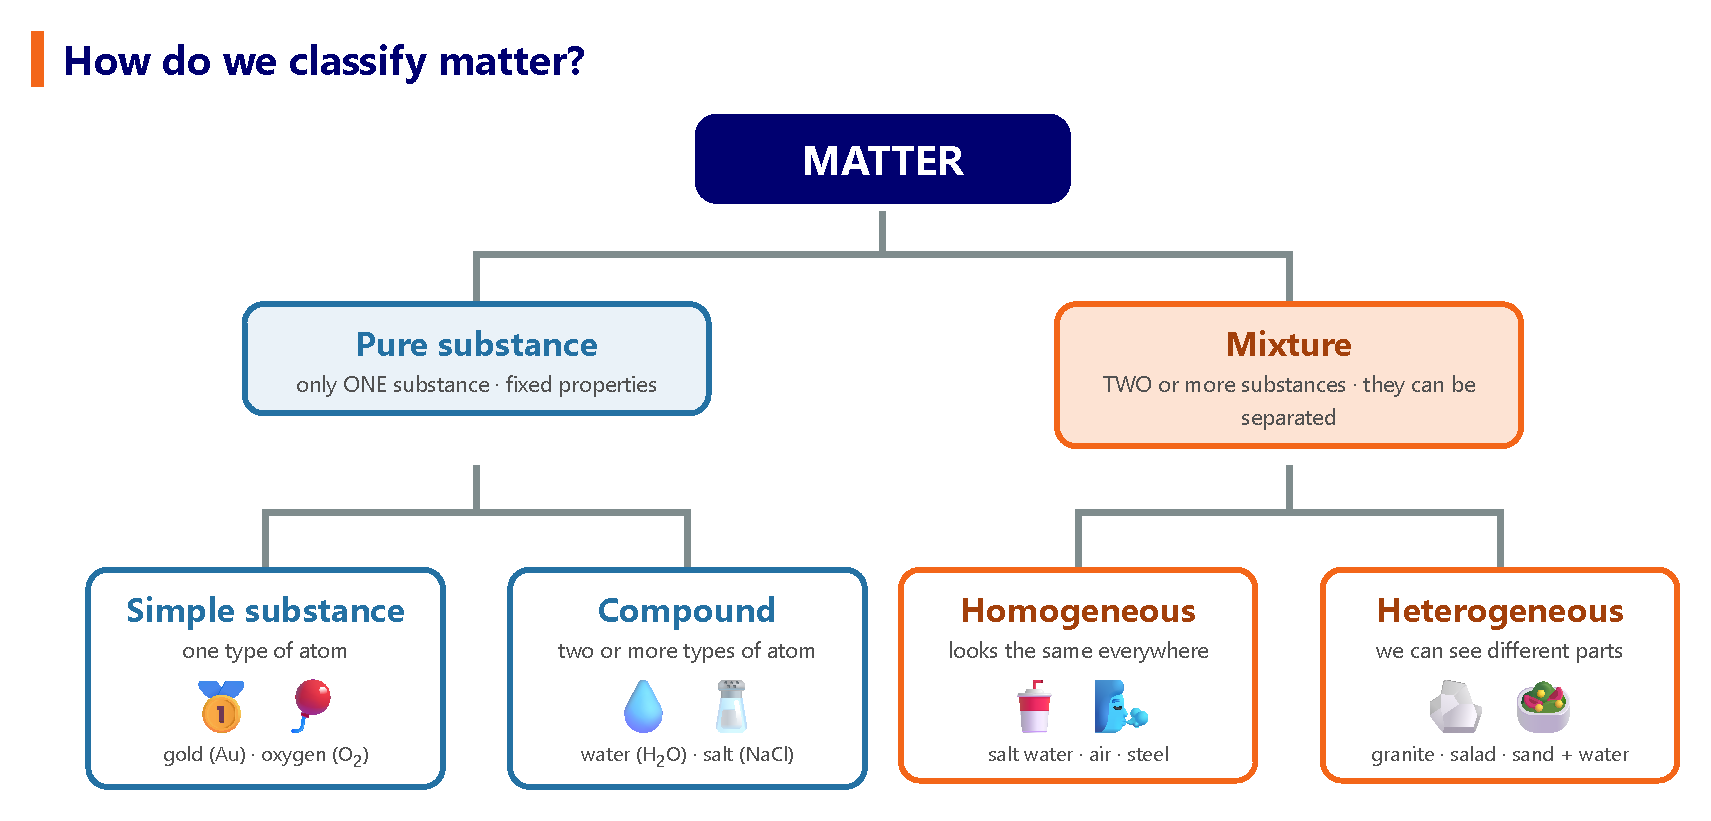
\includegraphics[width=\textwidth]{FigurasSVG/Unit_3_Diversity_of_Matter/pdf/matter_classification.pdf}
    \caption{Classification of matter.}
    \label{fig:u3_matter_classification}
\end{figure}

\begin{definition}[Pure substance]
    Matter made of \textbf{only one} substance. It has fixed, characteristic properties (for example, a fixed melting point). It can be a \textbf{simple substance} (one type of atom) or a \textbf{compound} (two or more types of atom).
\end{definition}

\begin{definition}[Mixture]
    Matter made of \textbf{two or more} substances. It is \textbf{homogeneous} if it looks the same everywhere (even with a microscope), and \textbf{heterogeneous} if we can see different parts.
\end{definition}

\begin{impt}
    \textbf{Pure substance or mixture?} Measure its melting point. Pure ice always melts at \qty{0}{\celsius}; different samples of butter (a mixture) melt at slightly different temperatures, because their composition is not fixed.
\end{impt}

\begin{exercise}
    Classify each example of matter according to its \textbf{appearance} (homogeneous or heterogeneous) and its \textbf{composition} (pure substance or mixture): sugar, salt water, granite, oxygen gas, milk.
    \begin{solu}
        \begin{center}
            \begin{tabular}{lll}
                \toprule
                \textbf{Matter} & \textbf{Appearance} & \textbf{Composition} \\
                \midrule
                Sugar & Homogeneous & Pure substance \\
                Salt water & Homogeneous & Mixture \\
                Granite & Heterogeneous & Mixture \\
                Oxygen gas & Homogeneous & Pure substance \\
                Milk & Looks homogeneous, but it is a colloid (heterogeneous) & Mixture \\
                \bottomrule
            \end{tabular}
        \end{center}
    \end{solu}
\end{exercise}

\begin{exercise}
    Say whether each example has a homogeneous or heterogeneous appearance: air, boiling water, smoke, yoghurt, sugar, crushed ice and lemon drink, milk and cocoa, paper with writing on it.
    \begin{solu}
        \textbf{Homogeneous}: air, sugar. \\
        \textbf{Heterogeneous}: boiling water (bubbles of gas in the liquid), smoke (solid particles in air), yoghurt, crushed ice and lemon drink, milk and cocoa, paper with writing on it.
    \end{solu}
\end{exercise}

\begin{exercise}
    Decide whether each system is a \textbf{pure substance} or a \textbf{mixture}, and justify your answer briefly: a) mineral water; b) oxygen gas (\ch{O2}); c) orange juice with pulp; d) sulphur powder (\ch{S}).
    \begin{solu}
        \begin{enumerate}[label=\alph*)]
            \item \textbf{Mixture}: water with several minerals dissolved in it.
            \item \textbf{Pure substance} (simple substance): only oxygen atoms.
            \item \textbf{Mixture} (heterogeneous): juice, water and visible pulp.
            \item \textbf{Pure substance} (simple substance): only sulphur atoms.
        \end{enumerate}
    \end{solu}
\end{exercise}

%----------------------------------------------------------------------------------------

\section{Homogeneous and heterogeneous mixtures}

Mixtures are classified by \textbf{what we can see}: can we tell their components apart just by looking at them, or not?

\subsection{Homogeneous mixtures}

\begin{definition}[Homogeneous mixture]
    A mixture whose components \textbf{cannot be distinguished with the naked eye}: it looks the same (uniform) in every part, and every sample of it has the same composition and the same properties.
\end{definition}

\begin{example}
    Some homogeneous mixtures we use every day:
    \begin{itemize}
        \item \textbf{Salt water} or \textbf{sugar dissolved in tea}: once the salt or the sugar has dissolved, we can no longer see it.
        \item \textbf{Air}: a mixture of nitrogen, oxygen, argon, carbon dioxide and other gases, but we cannot see any of them.
        \item \textbf{Mineral water} and \textbf{vinegar}: they look like a single clear liquid.
        \item \textbf{Steel} and \textbf{bronze}: metals mixed so well that they look like a single metal.
    \end{itemize}
\end{example}

The most important homogeneous mixtures are \textbf{solutions}, which we study in detail below.

\subsubsection{Solutions}

\begin{definition}[Solution]
    A \textbf{homogeneous} mixture of two or more substances. The \textbf{solvent} is the component in the largest amount; the \textbf{solute} (or solutes) is in a smaller amount.
\end{definition}

\begin{figure}[H]
    \centering
    % [FIGURA ORIGINAL] \includegraphics[width=\textwidth]{Unit_3/solution_parts}
    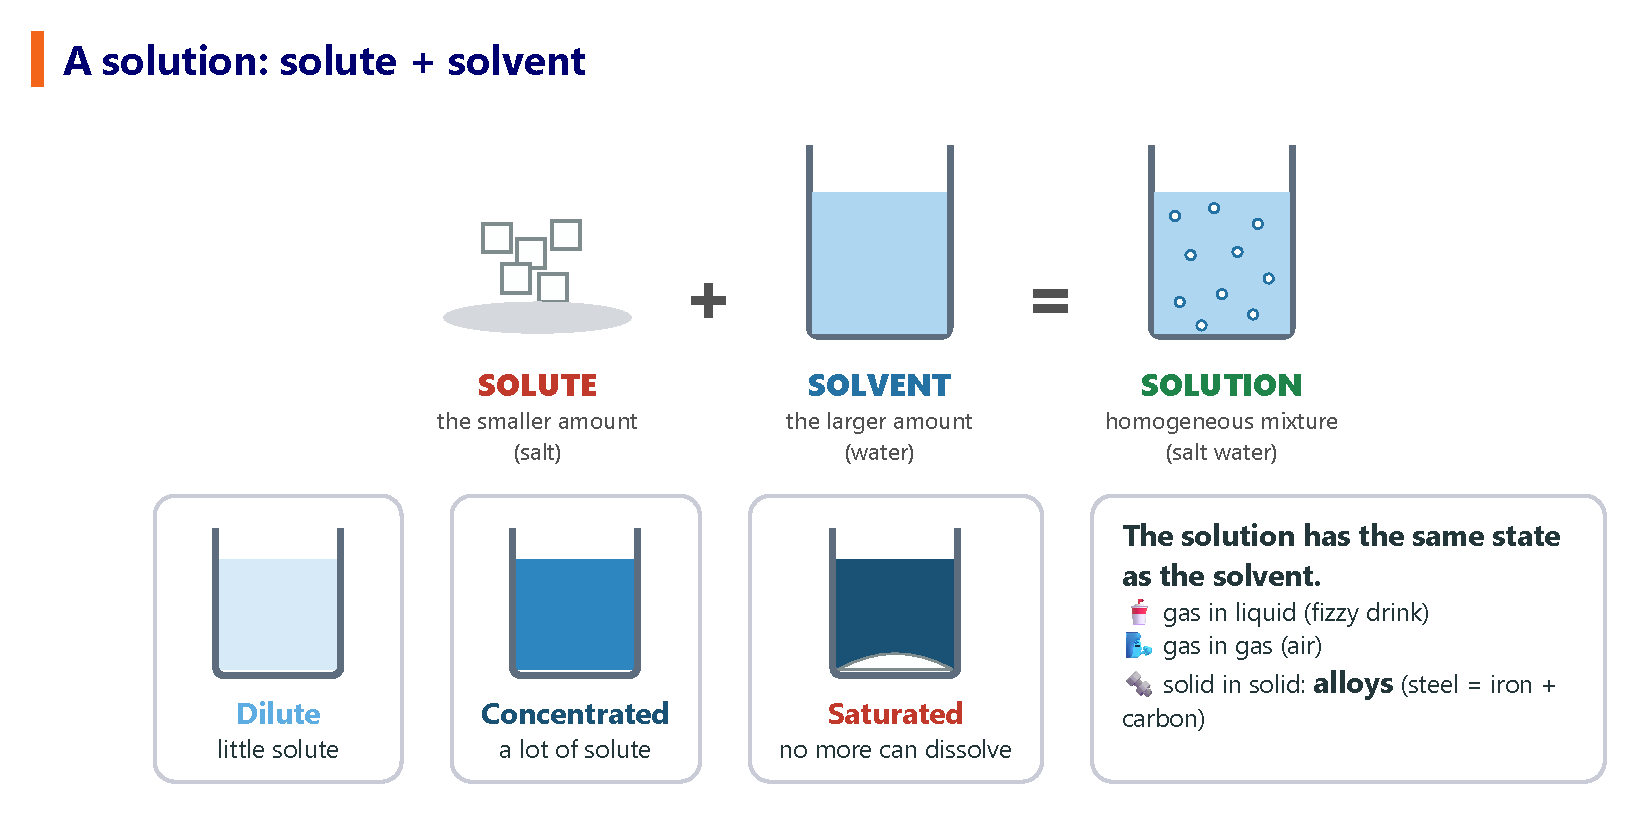
\includegraphics[width=\textwidth]{FigurasSVG/Unit_3_Diversity_of_Matter/pdf/solution_parts.pdf}
    \caption{The parts of a solution, and dilute, concentrated and saturated solutions.}
    \label{fig:u3_solution_parts}
\end{figure}

\begin{impt}
    A solution always has \textbf{one} solvent, but it can have \textbf{more than one solute}. For example:
    \begin{itemize}
        \item \textbf{Seawater}: the solvent is water, and the solutes are many different salts (sodium chloride, magnesium chloride, calcium sulfate\ldots).
        \item \textbf{A soft drink}: the solvent is water, and the solutes are sugar, carbon dioxide (the bubbles), colourings and flavourings.
        \item \textbf{Air}: the solvent is nitrogen, and the solutes are oxygen, argon, carbon dioxide and water vapour.
    \end{itemize}
\end{impt}

\begin{definition}[Alloy]
    A solid solution of two or more metals (or a metal and another element), made to improve the properties of the pure metal. Examples: steel (iron + carbon), bronze (copper + tin).
\end{definition}

\begin{exercise}
    For each mixture, indicate the physical state of the solute and of the solvent: air, sugar in water, steel, sparkling water, camomile tea.
    \begin{solu}
        \begin{center}
            \begin{tabular}{lll}
                \toprule
                \textbf{Mixture} & \textbf{Solute} & \textbf{Solvent} \\
                \midrule
                Air & Gas (oxygen, etc.) & Gas (nitrogen) \\
                Sugar in water & Solid & Liquid \\
                Steel & Solid (carbon) & Solid (iron) \\
                Sparkling water & Gas (\ch{CO2}) & Liquid \\
                Camomile tea & Solid/liquid & Liquid \\
                \bottomrule
            \end{tabular}
        \end{center}
    \end{solu}
\end{exercise}

\begin{exercise}
    A solution is made by mixing \qty{5}{\mL} of ethanol with \qty{45}{\mL} of water. Identify the solute and the solvent. Is this solution more or less concentrated than one made with \qty{20}{\mL} of ethanol and \qty{30}{\mL} of water?
    \begin{solu}
        Ethanol is in the smaller amount, so it is the \textbf{solute}; water is the \textbf{solvent}. \\
        The first solution has \qty{5}{\mL} of ethanol in \qty{50}{\mL}, and the second one \qty{20}{\mL} in \qty{50}{\mL}, so the first one is \textbf{more dilute} (less concentrated).
    \end{solu}
\end{exercise}

\begin{exercise}
    Give two examples of solutions found at home for each case: a) solid dissolved in liquid; b) liquid dissolved in liquid; c) gas dissolved in liquid.
    \begin{solu}
        \begin{enumerate}[label=\alph*)]
            \item Sugar in coffee; salt in soup.
            \item Vinegar (acetic acid in water); antifreeze in water.
            \item Sparkling water (\ch{CO2} in water); oxygen dissolved in the water of an aquarium.
        \end{enumerate}
    \end{solu}
\end{exercise}

\subsubsection{Concentration of solutions}

\begin{definition}[Concentration]
    The amount of solute dissolved in a given amount of solution.
\end{definition}

Before calculating any concentration, we must be very clear about what the \textbf{solution} is. The solution is \textbf{everything}: the solute (or solutes) \textbf{plus} the solvent.

\begin{figure}[H]
    \centering
    % [FIGURA ORIGINAL] \includegraphics[width=\textwidth]{Unit_3/solution_sum}
    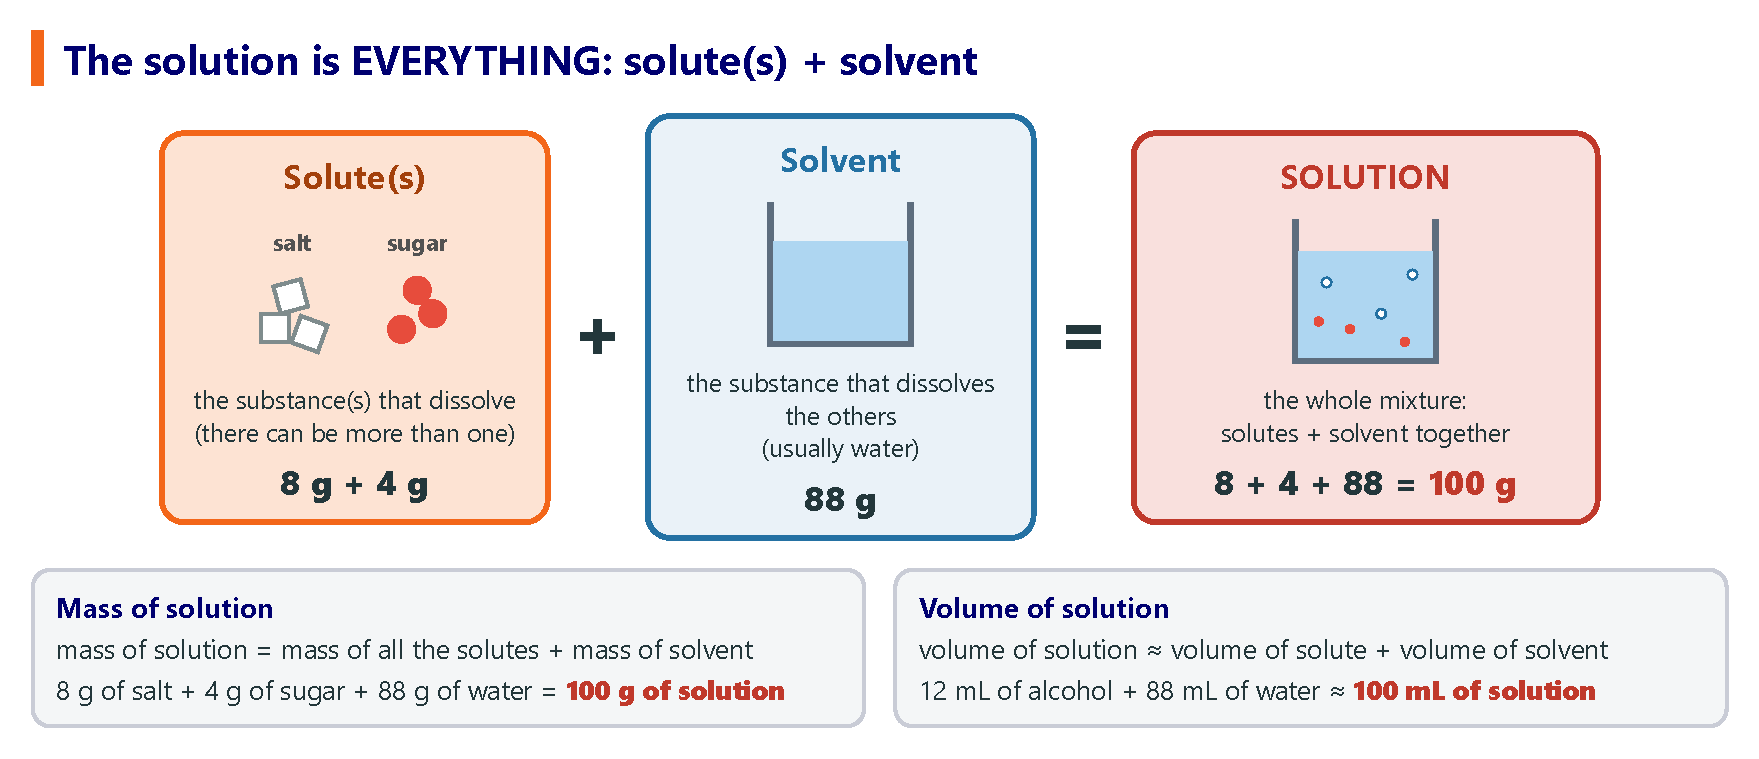
\includegraphics[width=\textwidth]{FigurasSVG/Unit_3_Diversity_of_Matter/pdf/solution_sum.pdf}
    \caption{The solution is the sum of all the solutes and the solvent.}
    \label{fig:u3_solution_sum}
\end{figure}

\begin{impt}
    \negsubro{Solution = solute(s) + solvent}
    \begin{equation*}
        \text{mass of solution} = \text{mass of solute(s)} + \text{mass of solvent}
    \end{equation*}
    \begin{equation*}
        \text{volume of solution} \approx \text{volume of solute} + \text{volume of solvent}
    \end{equation*}
    In all the formulas of concentration, the \textbf{solution} goes \textbf{below} the fraction line, \textbf{never} the solvent alone. If the exercise gives you the solute and the solvent separately, first \textbf{add them} to obtain the solution.
\end{impt}

We will use three ways of expressing the concentration of a solution:

\begin{figure}[H]
    \centering
    % [FIGURA ORIGINAL] \includegraphics[width=\textwidth]{Unit_3/concentration}
    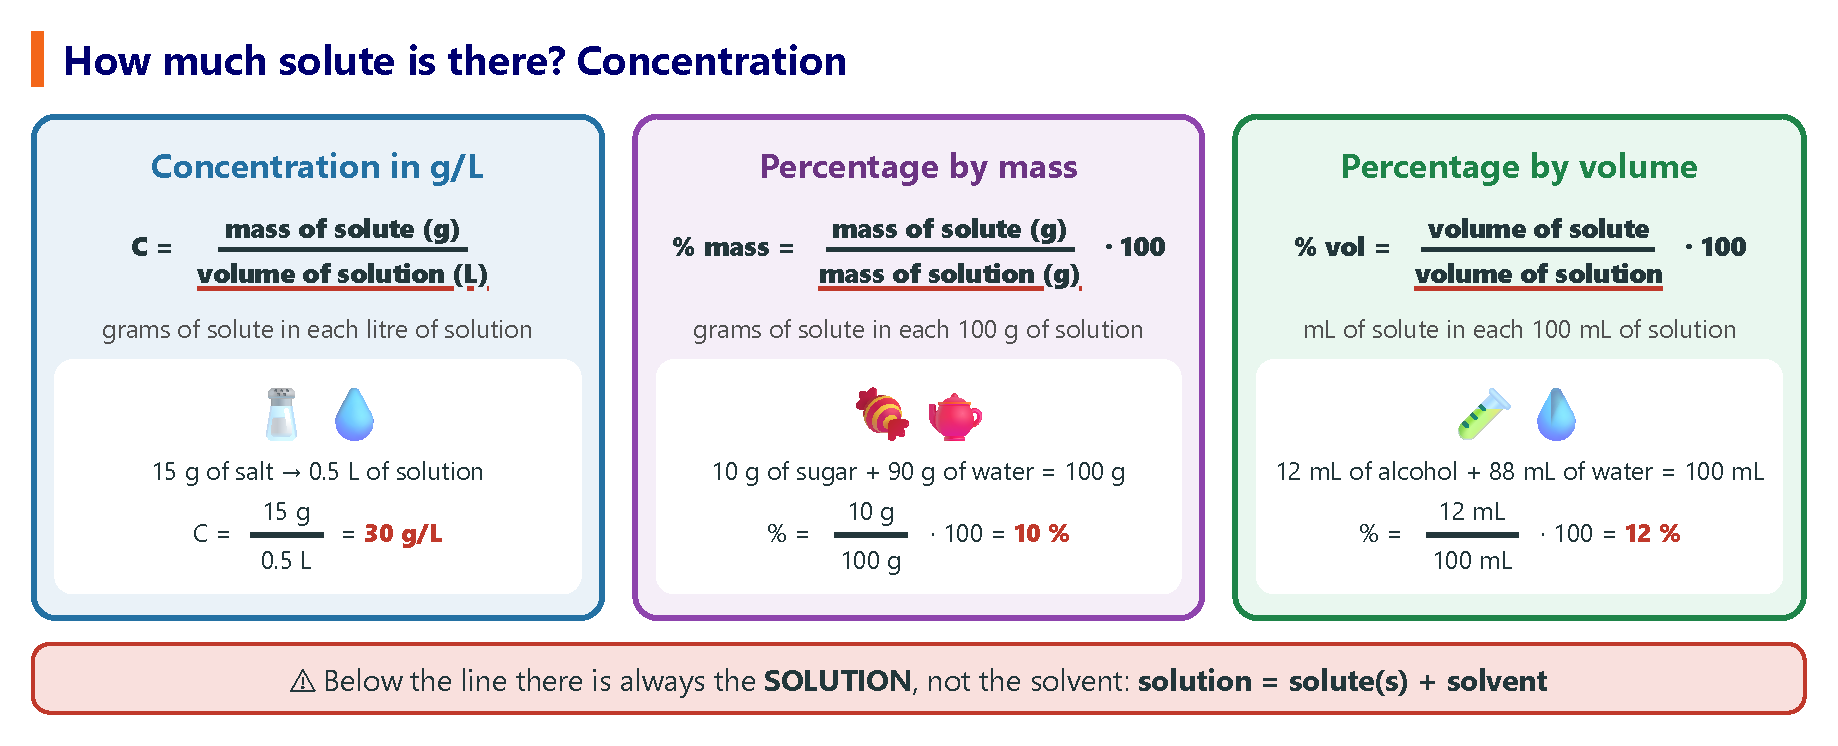
\includegraphics[width=\textwidth]{FigurasSVG/Unit_3_Diversity_of_Matter/pdf/concentration.pdf}
    \caption{Three ways of expressing concentration.}
    \label{fig:u3_concentration}
\end{figure}

\begin{equation*}
    C\,(\unit{\g\per\litre}) = \dfrac{\text{mass of solute (g)}}{\text{volume of solution (L)}}
\end{equation*}
\begin{equation*}
    \%\text{ mass} = \dfrac{\text{mass of solute (g)}}{\text{mass of solution (g)}} \cdot 100
    \qquad\qquad
    \%\text{ volume} = \dfrac{\text{volume of solute (mL)}}{\text{volume of solution (mL)}} \cdot 100
\end{equation*}

\begin{impt}
    \begin{itemize}
        \item The \textbf{concentration in g/L} tells us how many \textbf{grams} of solute there are in each \textbf{litre} of solution. The volume must be in \textbf{litres}.
        \item The \textbf{percentage by mass} tells us how many \textbf{grams} of solute there are in each \textbf{\qty{100}{\g}} of solution. Both masses must be in the \textbf{same unit}.
        \item The \textbf{percentage by volume} tells us how many \textbf{millilitres} of solute there are in each \textbf{\qty{100}{\mL}} of solution. It is used when the solute is a \textbf{liquid} (alcohol in wine, for example). Both volumes must be in the \textbf{same unit}.
    \end{itemize}
\end{impt}

\begin{example}
    \textbf{Concentration in g/L. \qty{15}{\g} of salt are dissolved in water to make \qty{500}{\mL} of solution. What is the concentration in g/L?}
    \begin{enumerate}[label=\numberballmDarkTeal]
        \item Data: mass of solute \(= \qty{15}{\g}\); volume of solution \(= \qty{500}{\mL}\). Unknown: \(C\).
        \item The volume must be in litres: \(\num{500}\,\unit{\mL} \cdot \dfrac{\qty{1}{\litre}}{\qty{e3}{\mL}} = \qty{0.5}{\litre}\).
        \item Formula: \(C = \dfrac{\text{mass of solute}}{\text{volume of solution}}\).
        \item \(C = \dfrac{\qty{15}{\g}}{\qty{0.5}{\litre}} = \textcolor{red}{\qty{30}{\g\per\litre}}\). There are \qty{30}{\g} of salt in each litre of solution.
    \end{enumerate}
\end{example}

\begin{example}
    \textbf{Percentage by mass. \qty{20}{\g} of sugar are dissolved in \qty{180}{\g} of water. What is the percentage by mass of sugar?}
    \begin{enumerate}[label=\numberballmDarkTeal]
        \item Data: mass of solute (sugar) \(= \qty{20}{\g}\); mass of \textbf{solvent} (water) \(= \qty{180}{\g}\). Unknown: \% mass.
        \item \textbf{Careful}: \qty{180}{\g} is the solvent, \textbf{not} the solution. We add them: \\
        mass of solution \(= \qty{20}{\g} + \qty{180}{\g} = \qty{200}{\g}\).
        \item Formula: \(\%\text{ mass} = \dfrac{\text{mass of solute}}{\text{mass of solution}} \cdot 100\).
        \item \(\%\text{ mass} = \dfrac{\qty{20}{\g}}{\qty{200}{\g}} \cdot 100 = \textcolor{red}{\qty{10}{\percent}}\). There are \qty{10}{\g} of sugar in each \qty{100}{\g} of solution.
    \end{enumerate}
\end{example}

\begin{example}
    \textbf{Percentage by volume. A solution is prepared by mixing \qty{30}{\mL} of alcohol with \qty{120}{\mL} of water. What is the percentage by volume of alcohol?}
    \begin{enumerate}[label=\numberballmDarkTeal]
        \item Data: volume of solute (alcohol) \(= \qty{30}{\mL}\); volume of \textbf{solvent} (water) \(= \qty{120}{\mL}\). Unknown: \% volume.
        \item Volume of solution \(= \qty{30}{\mL} + \qty{120}{\mL} = \qty{150}{\mL}\).
        \item Formula: \(\%\text{ volume} = \dfrac{\text{volume of solute}}{\text{volume of solution}} \cdot 100\).
        \item \(\%\text{ volume} = \dfrac{\qty{30}{\mL}}{\qty{150}{\mL}} \cdot 100 = \textcolor{red}{\qty{20}{\percent}}\). There are \qty{20}{\mL} of alcohol in each \qty{100}{\mL} of solution.
    \end{enumerate}
\end{example}

\begin{didyouknow}
    The labels of drinks show the percentage by volume of alcohol: ``13\,\% vol.'' on a bottle of wine means that each \qty{100}{\mL} of wine contain \qty{13}{\mL} of alcohol.
\end{didyouknow}

\begin{exercise}
    \textbf{Concentration in g/L.} Calculate:
    \begin{enumerate}[label=\letraminuscula]
        \item The concentration in g/L of a solution made by dissolving \qty{20}{\g} of sugar in water until the volume is \qty{400}{\mL}.
        \item The concentration in g/L of a solution that contains \qty{6}{\g} of salt in \qty{1.5}{\litre} of solution.
        \item The mass of salt in a \qty{500}{\mL} bottle of saline solution whose concentration is \qty{9}{\g\per\litre}.
    \end{enumerate}
    \begin{solu}
        \begin{enumerate}[label=\alph*)]
            \item \(V = \qty{400}{\mL} = \qty{0.4}{\litre}\); \(C = \dfrac{\qty{20}{\g}}{\qty{0.4}{\litre}} = \qty{50}{\g\per\litre}\).
            \item \(C = \dfrac{\qty{6}{\g}}{\qty{1.5}{\litre}} = \qty{4}{\g\per\litre}\).
            \item \(V = \qty{0.5}{\litre}\); mass of solute \(= C \cdot V = \qty{9}{\g\per\litre} \cdot \qty{0.5}{\litre} = \qty{4.5}{\g}\).
        \end{enumerate}
    \end{solu}
\end{exercise}

\begin{exercise}
    \textbf{Percentage by mass.} Calculate:
    \begin{enumerate}[label=\letraminuscula]
        \item The percentage by mass of a solution made with \qty{15}{\g} of salt and \qty{135}{\g} of water.
        \item The percentage by mass of each solute in a solution made with \qty{2}{\g} of salt, \qty{3}{\g} of sugar and \qty{95}{\g} of water.
        \item The mass of solute and the mass of water in \qty{300}{\g} of a solution at \qty{5}{\percent} by mass.
    \end{enumerate}
    \begin{solu}
        \begin{enumerate}[label=\alph*)]
            \item Mass of solution \(= 15 + 135 = \qty{150}{\g}\); \(\%\text{ mass} = \dfrac{\qty{15}{\g}}{\qty{150}{\g}} \cdot 100 = \qty{10}{\percent}\).
            \item Mass of solution \(= 2 + 3 + 95 = \qty{100}{\g}\) (all the solutes and the solvent). Salt: \(\dfrac{\qty{2}{\g}}{\qty{100}{\g}} \cdot 100 = \qty{2}{\percent}\); sugar: \(\dfrac{\qty{3}{\g}}{\qty{100}{\g}} \cdot 100 = \qty{3}{\percent}\).
            \item Mass of solute \(= \qty{300}{\g} \cdot \dfrac{5}{100} = \qty{15}{\g}\); mass of water \(= 300 - 15 = \qty{285}{\g}\).
        \end{enumerate}
    \end{solu}
\end{exercise}

\begin{exercise}
    \textbf{Percentage by volume.} Calculate:
    \begin{enumerate}[label=\letraminuscula]
        \item The percentage by volume of a solution made by mixing \qty{30}{\mL} of alcohol with \qty{220}{\mL} of water.
        \item The volume of alcohol in a \qty{750}{\mL} bottle of wine labelled ``\qty{13}{\percent} vol.''.
        \item A hand sanitiser gel has \qty{70}{\percent} alcohol by volume. How many millilitres of alcohol and of water are there in a \qty{200}{\mL} bottle?
    \end{enumerate}
    \begin{solu}
        \begin{enumerate}[label=\alph*)]
            \item Volume of solution \(= 30 + 220 = \qty{250}{\mL}\); \(\%\text{ volume} = \dfrac{\qty{30}{\mL}}{\qty{250}{\mL}} \cdot 100 = \qty{12}{\percent}\).
            \item Volume of alcohol \(= \qty{750}{\mL} \cdot \dfrac{13}{100} = \qty{97.5}{\mL}\).
            \item Alcohol: \(\qty{200}{\mL} \cdot \dfrac{70}{100} = \qty{140}{\mL}\); water: \(200 - 140 = \qty{60}{\mL}\).
        \end{enumerate}
    \end{solu}
\end{exercise}

%\begin{definition}[Solubility]
%    The \textbf{maximum} amount of solute that can dissolve in a given amount of solvent, at a given temperature. A solution with this maximum amount is \textbf{saturated}: any extra solute stays at the bottom.
%\end{definition}

%\begin{figure}[H]
%    \centering
%    % [FIGURA ORIGINAL] \includegraphics[width=\textwidth]{Unit_3/solubility_graph}
%    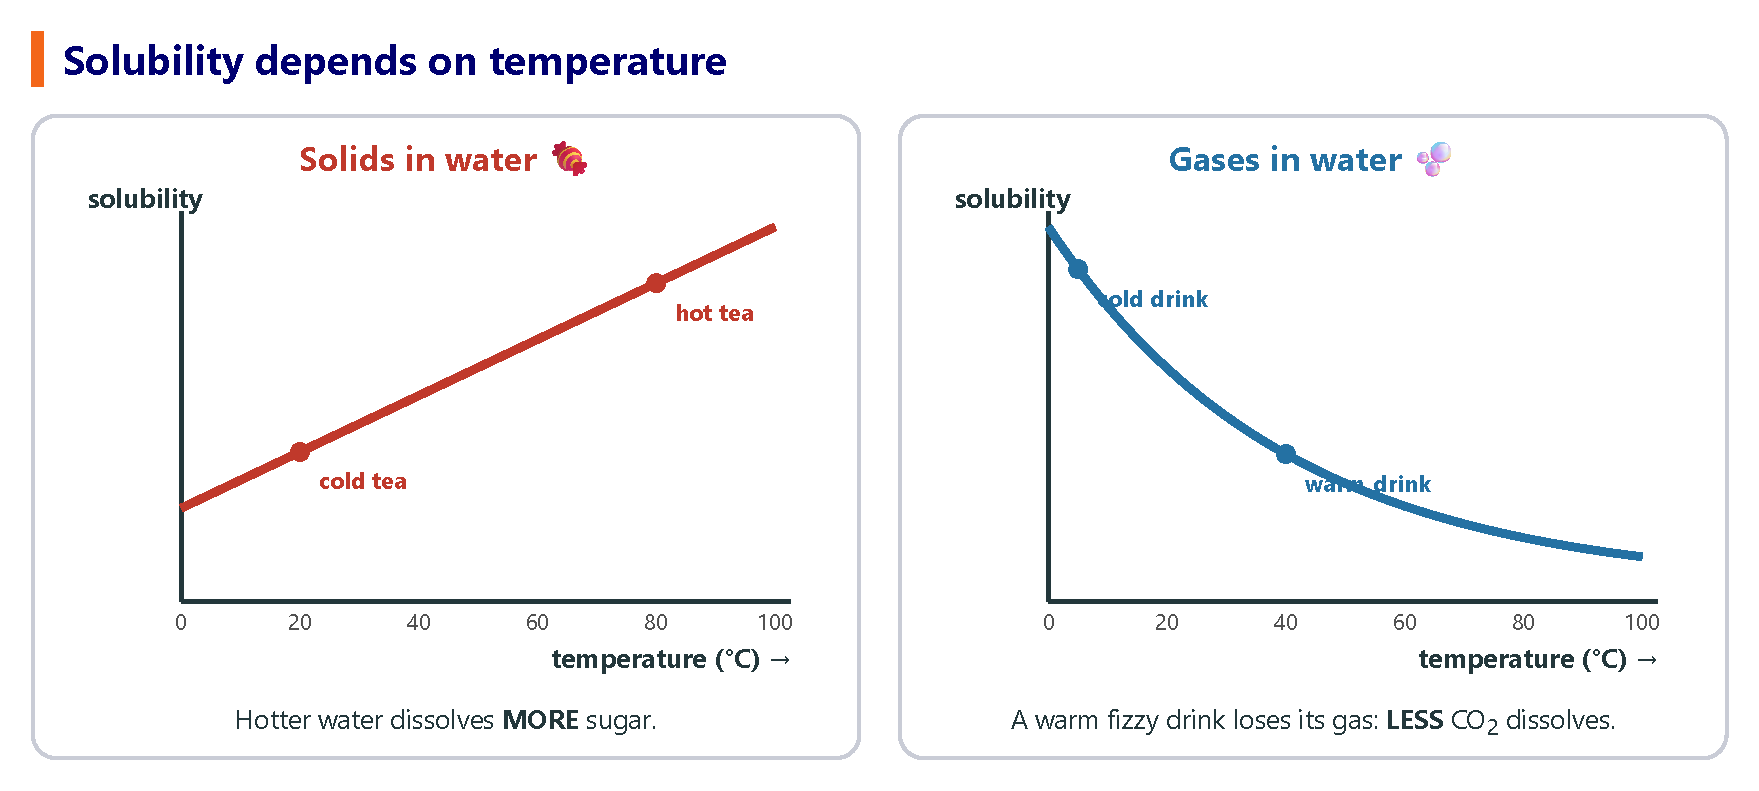
\includegraphics[width=\textwidth]{FigurasSVG/Unit_3_Diversity_of_Matter/pdf/solubility_graph.pdf}
%    \caption{Temperature increases the solubility of most solids, but decreases the solubility of gases.}
%    \label{fig:u3_solubility_graph}
%\end{figure}

%\begin{impt}
%    Solubility depends on:
%    \begin{itemize}
%        \item \textbf{The substances}: salt and sugar dissolve in water; oil and sand do not.
%        \item \textbf{Temperature}: see the graphs above.
%        \item \textbf{Stirring} does \emph{not} change the solubility, but it makes the solute dissolve \textbf{faster}.
%    \end{itemize}
%\end{impt}

\begin{exercise}
    \qty{25}{\g} of sugar are dissolved in water to make \qty{250}{\mL} of solution. Calculate the concentration of the solution in g/L.
    \begin{solu}
        \(V = \qty{250}{\mL} = \qty{0.250}{\litre}\); \quad \(C = \dfrac{\qty{25}{\g}}{\qty{0.250}{\litre}} = \qty{100}{\g\per\litre}\).
    \end{solu}
\end{exercise}

\begin{exercise}
    A solution is prepared by dissolving \qty{8}{\g} of salt in \qty{92}{\g} of water.
    \begin{enumerate}[label=\letraminuscula]
        \item Calculate the percentage by mass of the solution.
        \item If we had \qty{500}{\g} of this same solution, what mass of salt would it contain?
    \end{enumerate}
    \begin{solu}
        \begin{enumerate}[label=\alph*)]
            \item Mass of solution \(= \qty{8}{\g} + \qty{92}{\g} = \qty{100}{\g}\); \quad \(\% \text{ mass} = \dfrac{\qty{8}{\g}}{\qty{100}{\g}} \cdot 100 = \qty{8}{\percent}\).
            \item \(\qty{500}{\g} \cdot \dfrac{8}{100} = \qty{40}{\g}\) of salt.
        \end{enumerate}
    \end{solu}
\end{exercise}

\begin{exercise}
    Explain, using the idea of solubility, why sugar dissolves better in hot tea than in cold tea, and why a can of fizzy drink loses its bubbles faster when it is left open on a warm day.
    \begin{solu}
        The solubility of a solid such as sugar \textbf{increases} with temperature, so more sugar dissolves in hot tea. \\
        The solubility of a gas such as \ch{CO2} \textbf{decreases} with temperature: as the drink warms up, less gas can stay dissolved, and it escapes as bubbles.
    \end{solu}
\end{exercise}

\begin{exercise}
    A bottle contains \qty{750}{\mL} of a solution with a concentration of \qty{40}{\g\per\litre}. Calculate the mass of solute dissolved in the bottle.
    \begin{solu}
        \(\text{mass} = C \cdot V = \qty{40}{\g\per\litre} \cdot \qty{0.750}{\litre} = \qty{30}{\g}\) of solute.
    \end{solu}
\end{exercise}

\begin{exercise}
    A solution is prepared by dissolving \qty{12}{\g} of salt in enough water to make \qty{200}{\g} of solution.
    \begin{enumerate}[label=\letraminuscula]
        \item Calculate the percentage by mass of the solution.
        \item What mass of this solution would you need in order to have \qty{6}{\g} of salt?
    \end{enumerate}
    \begin{solu}
        \begin{enumerate}[label=\alph*)]
            \item \(\% \text{ mass} = \dfrac{\qty{12}{\g}}{\qty{200}{\g}} \cdot 100 = \qty{6}{\percent}\).
            \item \(\qty{6}{\g} \cdot \dfrac{100}{6} = \qty{100}{\g}\) of solution.
        \end{enumerate}
    \end{solu}
\end{exercise}

\subsection{Heterogeneous mixtures}

\begin{definition}[Heterogeneous mixture]
    A mixture whose components \textbf{can be distinguished with the naked eye}: we can see different parts in it, and two samples taken from different places may have a different composition.
\end{definition}

\begin{example}
    Some heterogeneous mixtures:
    \begin{itemize}
        \item \textbf{Granite}: we can see grains of three different minerals (white, black and pink or grey).
        \item \textbf{Sand and water}, or \textbf{muddy water}: the sand or the mud can be seen, and it settles at the bottom.
        \item \textbf{Oil and water}: two layers, with the oil on top.
        \item \textbf{A salad}, \textbf{paella} or \textbf{a pizza}: each ingredient can be recognised.
    \end{itemize}
\end{example}

Some heterogeneous mixtures are special: their components are so small that, with the naked eye, the mixture \textbf{looks} homogeneous, and we need a microscope to see its different parts. These are the \textbf{colloids}.

\subsubsection{Colloids}

\begin{definition}[Colloid]
    A heterogeneous mixture that \textbf{looks} homogeneous to the naked eye, but in which we can see particles of different composition under a microscope. Examples: milk, blood, mayonnaise, gelatine, fog.
\end{definition}

\begin{definition}[Tyndall effect]
    The scattering of light by the particles of a colloid, which makes a beam of light visible inside it. Solutions do \textbf{not} show this effect.
\end{definition}

\begin{figure}[H]
    \centering
    % [FIGURA ORIGINAL] \includegraphics[width=\textwidth]{Unit_3/tyndall}
    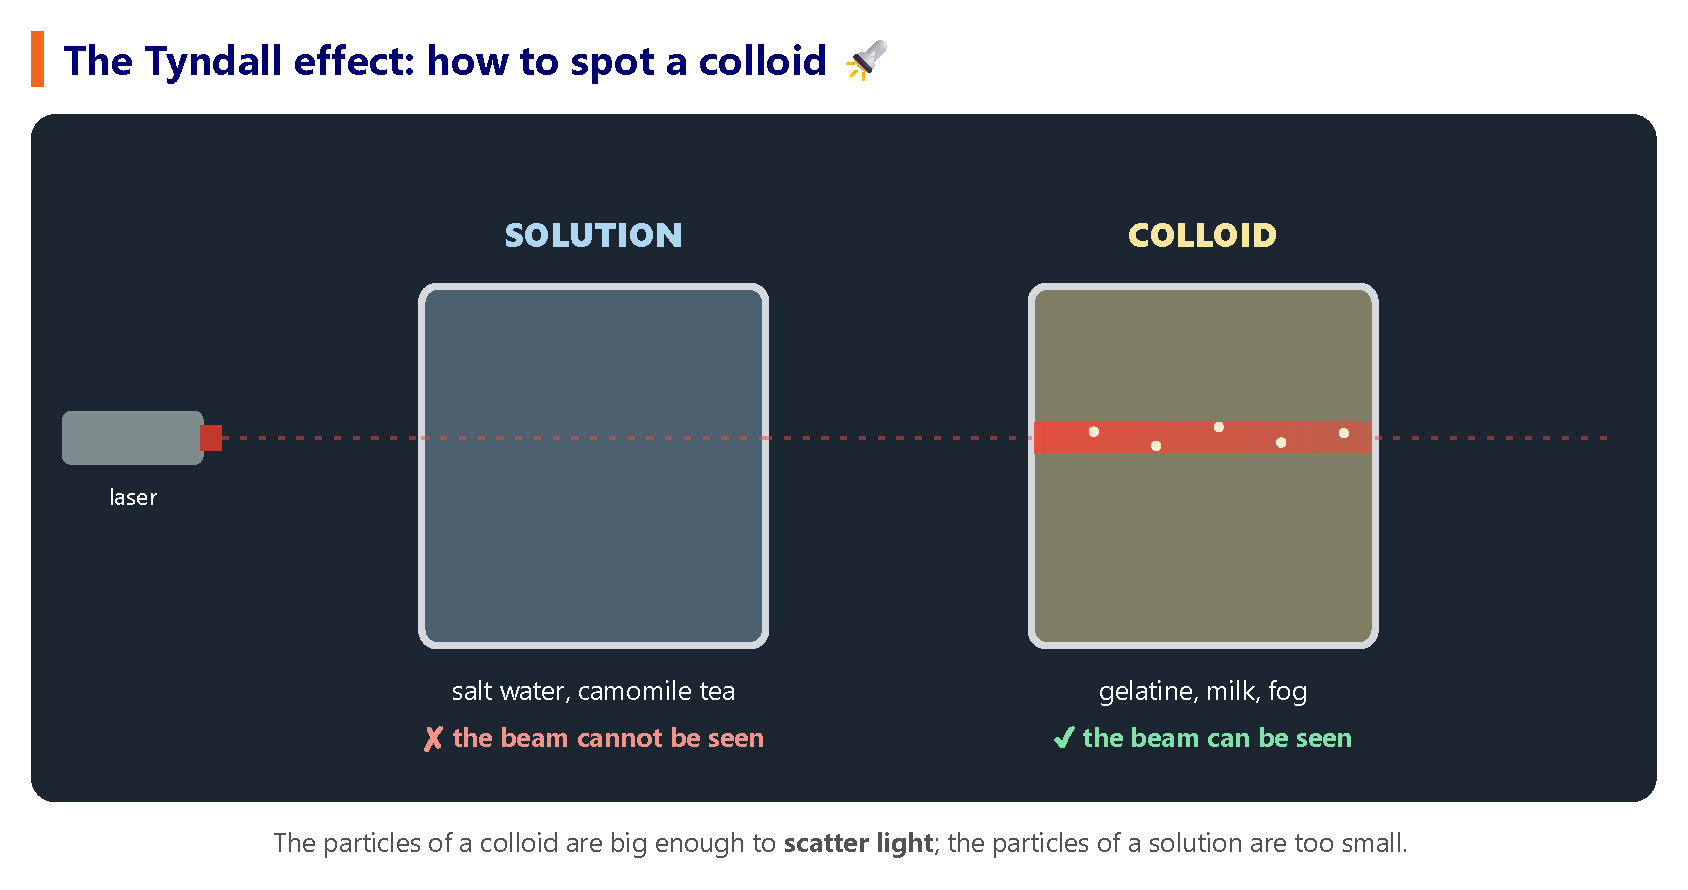
\includegraphics[width=\textwidth]{FigurasSVG/Unit_3_Diversity_of_Matter/pdf/tyndall.pdf}
    \caption{The Tyndall effect lets us tell a colloid from a solution.}
    \label{fig:u3_tyndall}
\end{figure}

\begin{didyouknow}
    When sunbeams come through the trees on a foggy morning, or through the window of a dusty room, you are seeing the Tyndall effect! Fog and dusty air are colloids, and their particles scatter the sunlight.
\end{didyouknow}

\begin{exercise}
    Explain why a solution of copper sulphate in water does not show the Tyndall effect, while a mixture of gelatine in water does.
    \begin{solu}
        In the copper sulphate solution the dissolved particles are extremely small, too small to scatter light, so the beam is not visible. In gelatine, the particles are larger (colloid size) and scatter the light, so the beam can be seen: this is the \textbf{Tyndall effect}.
    \end{solu}
\end{exercise}

\begin{exercise}
    Classify each mixture as a \textbf{solution} or a \textbf{colloid}, giving a reason based on particle size: mayonnaise, sea water, whipped cream, vinegar.
    \begin{solu}
        Mayonnaise: \textbf{colloid} (oil droplets dispersed in water). \\
        Sea water: \textbf{solution} (dissolved salts, very small particles). \\
        Whipped cream: \textbf{colloid} (tiny air bubbles and fat droplets). \\
        Vinegar: \textbf{solution} (acetic acid dissolved in water).
    \end{solu}
\end{exercise}

\subsubsection{Emulsions}

\begin{definition}[Emulsion]
    A colloid made of two liquids that do not mix (such as oil and water), kept together by a third substance called an \textbf{emulsifier}.
\end{definition}

\begin{figure}[H]
    \centering
    % [FIGURA ORIGINAL] \includegraphics[width=\textwidth]{Unit_3/emulsion}
    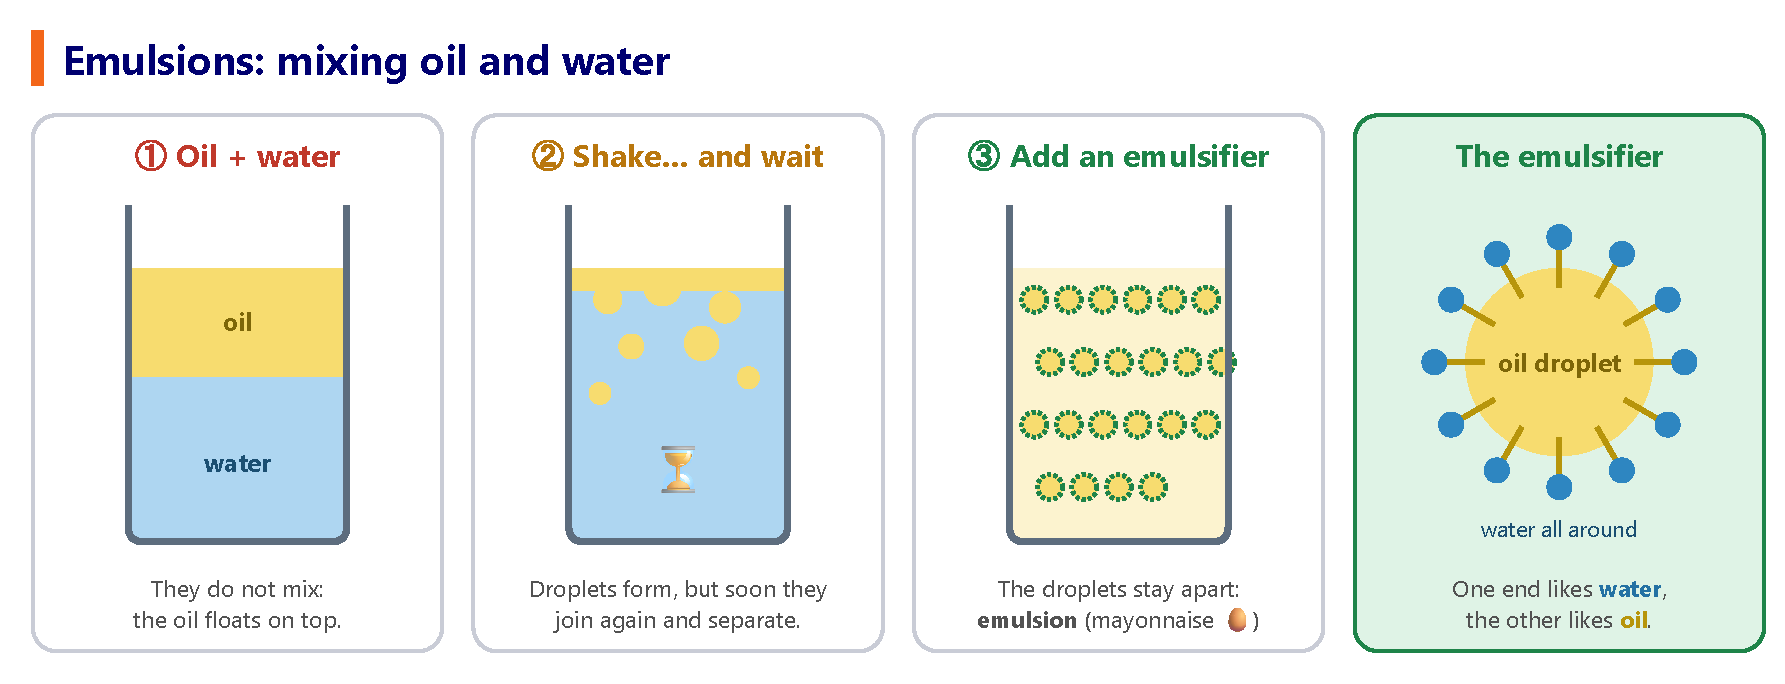
\includegraphics[width=\textwidth]{FigurasSVG/Unit_3_Diversity_of_Matter/pdf/emulsion.pdf}
    \caption{An emulsifier keeps the oil droplets apart inside the water.}
    \label{fig:u3_emulsion}
\end{figure}

\begin{example}
    In mayonnaise the emulsifier is \textbf{lecithin}, from egg yolk; in milk it is \textbf{casein}, a milk protein. Soap also works as an emulsifier: that is why it removes grease from your hands.
\end{example}

\begin{exercise}
    Explain what happens if you shake a mixture of oil and water \textbf{without} adding any emulsifier, and why.
    \begin{solu}
        Shaking breaks the oil into small droplets, but without an emulsifier nothing keeps them apart. The droplets join together again and the mixture separates into two layers, with the less dense oil on top.
    \end{solu}
\end{exercise}

\begin{exercise}
    Identify the emulsifier in each emulsion: a) mayonnaise; b) milk; c) many cosmetic creams.
    \begin{solu}
        \begin{enumerate}[label=\alph*)]
            \item Lecithin, from egg yolk.
            \item Casein, a milk protein.
            \item Emulsifying waxes or soap-like molecules, with one end that mixes with water and the other with oil.
        \end{enumerate}
    \end{solu}
\end{exercise}

\subsection{Particle size and types of mixtures}

\begin{figure}[H]
    \centering
    % [FIGURA ORIGINAL] \includegraphics[width=\textwidth]{Unit_3/particle_size}
    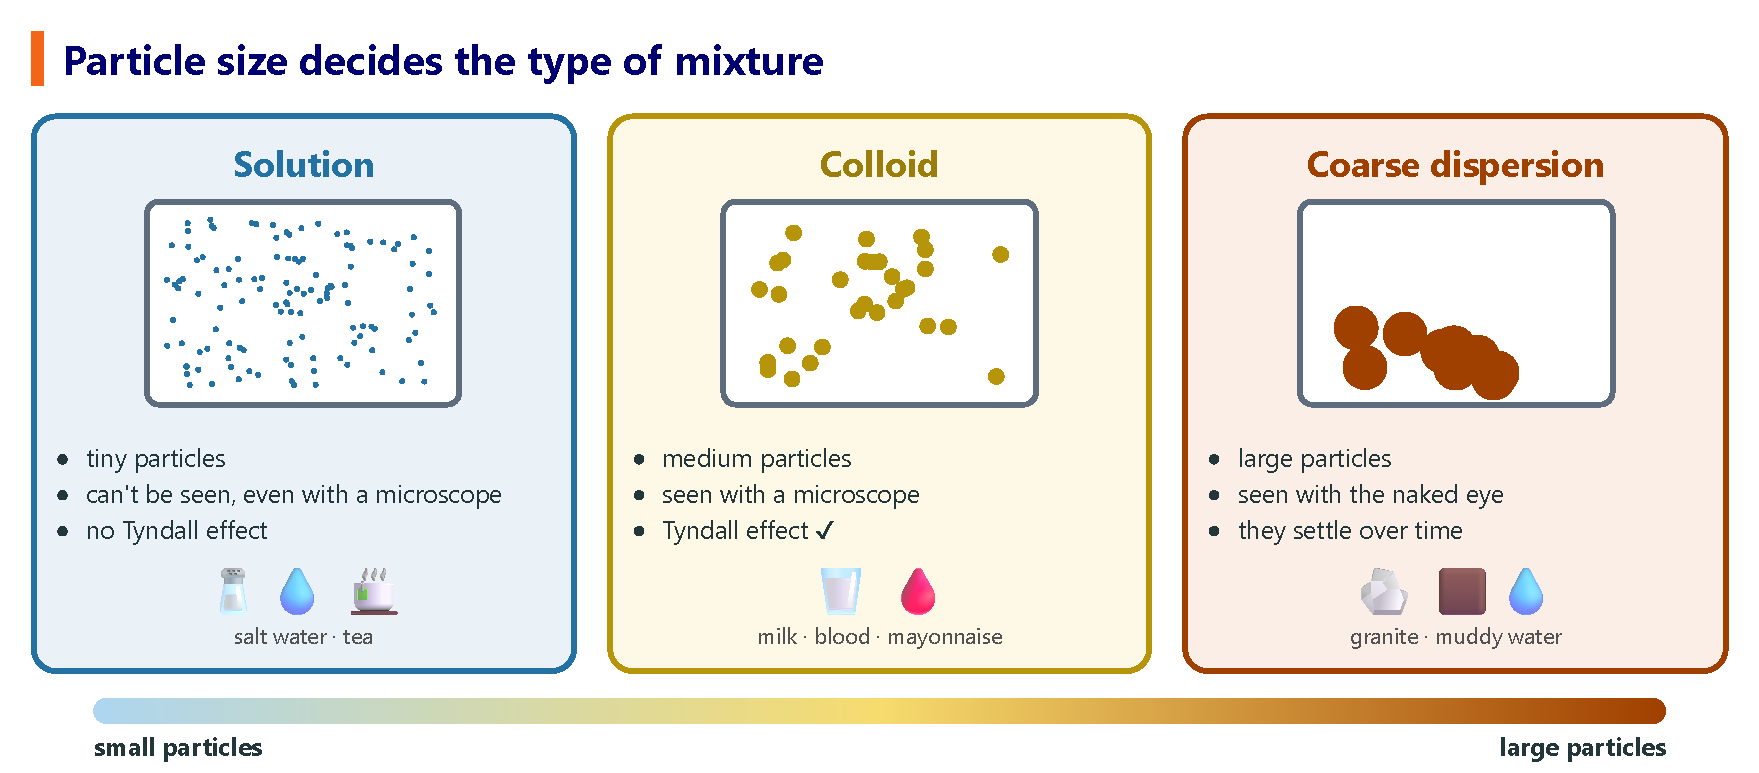
\includegraphics[width=\textwidth]{FigurasSVG/Unit_3_Diversity_of_Matter/pdf/particle_size.pdf}
    \caption{The bigger the dispersed particles, the more heterogeneous the mixture.}
    \label{fig:u3_particle_size}
\end{figure}

\begin{exercise}
    Classify these mixtures as homogeneous or heterogeneous, and say if they are colloids: meringue, physiological saline solution, coins (metal alloy), marble, milk, fizzy drinks.
    \begin{solu}
        Meringue: \textbf{heterogeneous}, colloid (air trapped in egg white). \\
        Physiological saline solution: \textbf{homogeneous} (a solution). \\
        Coins: \textbf{homogeneous} (an alloy, a solid solution). \\
        Marble: \textbf{heterogeneous} (we can see veins and grains). \\
        Milk: \textbf{heterogeneous}, colloid, although it looks homogeneous. \\
        Fizzy drinks: \textbf{homogeneous} (a solution of \ch{CO2} in water).
    \end{solu}
\end{exercise}

\begin{exercise}
    Order these three systems from \textbf{smallest} to \textbf{largest} dispersed-particle size, and name the type of mixture each one is: sugar solution, muddy river water, milk.
    \begin{solu}
        \textbf{Sugar solution} (solution) \(<\) \textbf{milk} (colloid) \(<\) \textbf{muddy river water} (coarse dispersion).
    \end{solu}
\end{exercise}

%----------------------------------------------------------------------------------------

\section{What makes up matter}

\begin{definition}[Atom]
    The tiny particle that makes up all matter. Atoms are made of even smaller particles: \textbf{protons}, \textbf{neutrons} and \textbf{electrons}.
\end{definition}

Scientists could not see atoms, so they imagined \textbf{models} to explain the results of their experiments. Each new experiment improved the model:

\begin{figure}[H]
    \centering
    % [FIGURA ORIGINAL] \includegraphics[width=\textwidth]{Unit_3/atomic_models}
    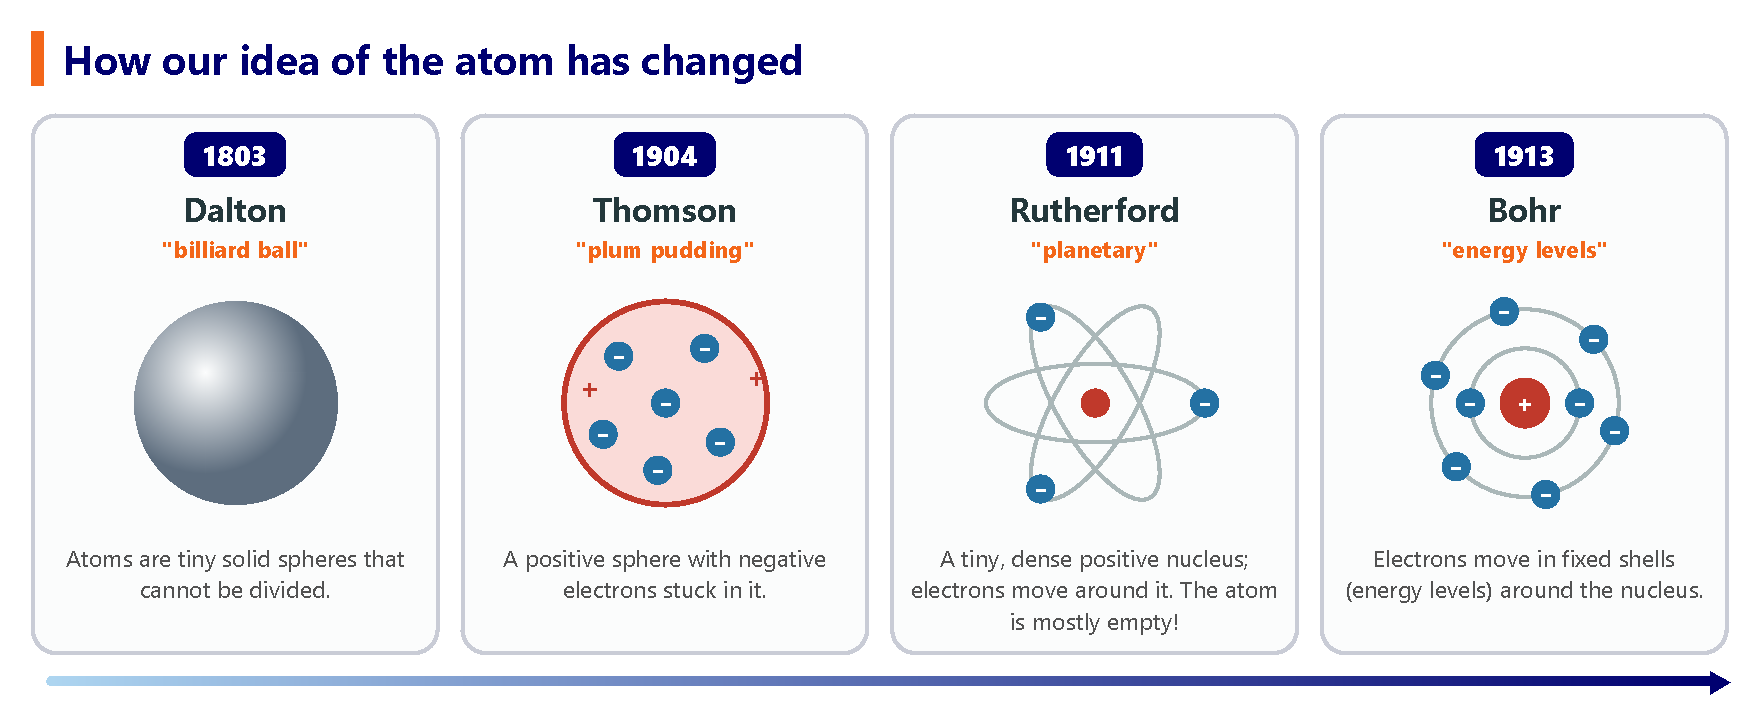
\includegraphics[width=\textwidth]{FigurasSVG/Unit_3_Diversity_of_Matter/pdf/atomic_models.pdf}
    \caption{The main atomic models.}
    \label{fig:u3_atomic_models}
\end{figure}

\begin{didyouknow}
    The atom is almost completely empty! If the nucleus were the size of a football in the centre of a stadium, the electrons would be like tiny grains of sand moving around the last rows of seats. Rutherford discovered this in 1911, when he fired particles at a very thin sheet of gold and almost all of them went straight through.
\end{didyouknow}

\subsection{The structure of the atom}

\begin{figure}[H]
    \centering
    % [FIGURA ORIGINAL] \includegraphics[width=\textwidth]{Unit_3/atom_structure}
    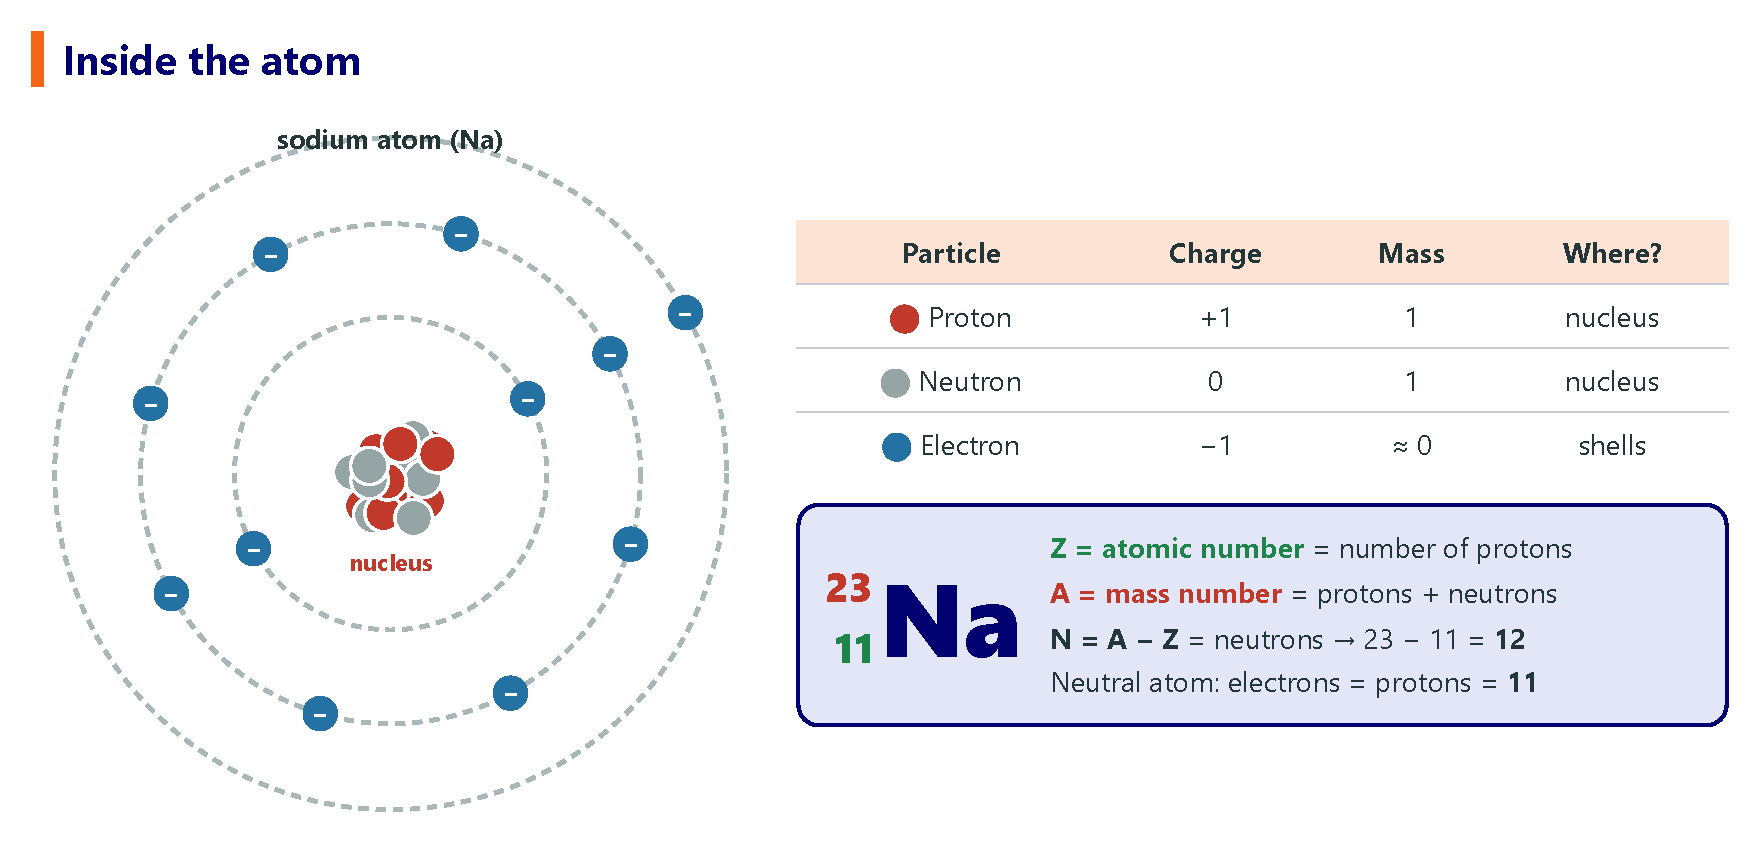
\includegraphics[width=\textwidth]{FigurasSVG/Unit_3_Diversity_of_Matter/pdf/atom_structure.pdf}
    \caption{The particles of the atom and how we represent an atom.}
    \label{fig:u3_atom_structure}
\end{figure}

\begin{impt}
    Almost all the \textbf{mass} of the atom is in the \textbf{nucleus}; almost all its \textbf{volume} is the space where the electrons move. In a \textbf{neutral} atom, number of electrons \(=\) number of protons.
\end{impt}

\begin{definition}[Atomic number \(Z\) and mass number \(A\)]
    \(Z\) is the number of \textbf{protons}: it tells us which element the atom is. \(A\) is the number of protons \textbf{plus} neutrons. So the number of neutrons is
    \begin{equation*}
        N = A - Z
    \end{equation*}
\end{definition}

\begin{example}
    Sodium, \ch{^{23}_{11}Na}: \(Z = 11\) and \(A = 23\). It has 11 protons, 11 electrons (it is neutral) and \(N = 23 - 11 = 12\) neutrons.
\end{example}

\begin{definition}[Isotopes]
    Atoms of the \textbf{same} element (same \(Z\)) with a \textbf{different} number of neutrons (different \(A\)).
\end{definition}

\begin{figure}[H]
    \centering
    % [FIGURA ORIGINAL] \includegraphics[width=0.9\textwidth]{Unit_3/isotopes}
    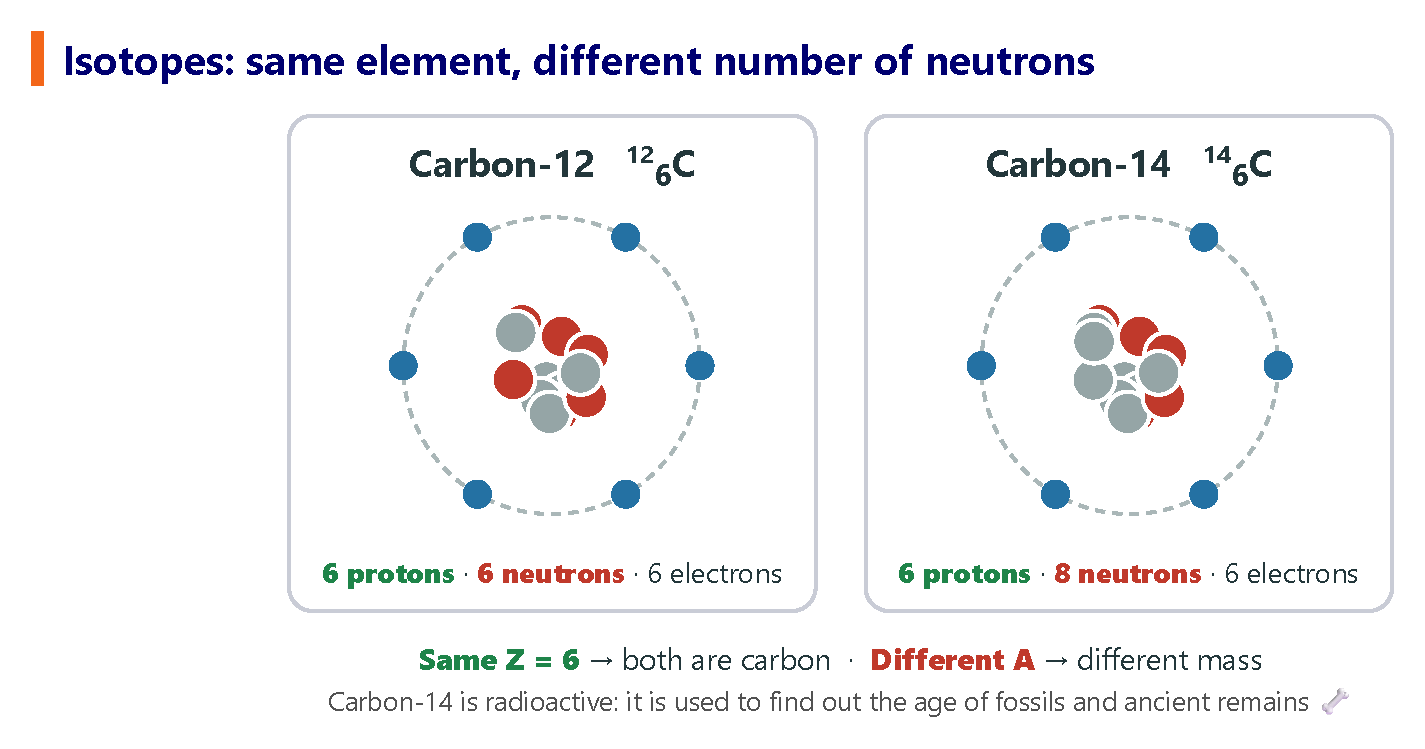
\includegraphics[width=0.9\textwidth]{FigurasSVG/Unit_3_Diversity_of_Matter/pdf/isotopes.pdf}
    \caption{Two isotopes of carbon.}
    \label{fig:u3_isotopes}
\end{figure}

\begin{exercise}
    An atom has 17 protons, 17 electrons and 18 neutrons.
    \begin{enumerate}[label=\letraminuscula]
        \item Give its atomic number \(Z\) and its mass number \(A\).
        \item Which chemical element is it? (Hint: atomic number 17 is chlorine.)
    \end{enumerate}
    \begin{solu}
        \begin{enumerate}[label=\alph*)]
            \item \(Z = 17\); \(A = 17 + 18 = 35\).
            \item \textbf{Chlorine}, \ch{Cl}.
        \end{enumerate}
    \end{solu}
\end{exercise}

\begin{exercise}
    Two isotopes of an element have mass numbers 35 and 37, and both have \(Z = 17\). Explain what they have in common and what makes them different.
    \begin{solu}
        Both have 17 protons and 17 electrons (same element). They have a different number of neutrons: \(N = 35 - 17 = 18\) and \(N = 37 - 17 = 20\).
    \end{solu}
\end{exercise}

\begin{exercise}
    Complete the table for these neutral atoms:
    \begin{center}
        \renewcommand{\arraystretch}{1.3}
        \begin{tabular}{cccccc}
            \toprule
            \textbf{Element} & \(Z\) & \(A\) & \textbf{Protons} & \textbf{Neutrons} & \textbf{Electrons} \\
            \midrule
            Oxygen & 8 & 16 & & & \\
            Magnesium & 12 & 24 & & & \\
            Potassium & 19 & 39 & & & \\
            \bottomrule
        \end{tabular}
    \end{center}
    \begin{solu}
        Oxygen: 8 protons, \(16 - 8 = 8\) neutrons, 8 electrons. \\
        Magnesium: 12 protons, \(24 - 12 = 12\) neutrons, 12 electrons. \\
        Potassium: 19 protons, \(39 - 19 = 20\) neutrons, 19 electrons.
    \end{solu}
\end{exercise}

\begin{exercise}
    Potassium-40 (\(Z = 19\), \(A = 40\)) and calcium-40 (\(Z = 20\), \(A = 40\)) have the same mass number. Explain why they are \textbf{not} isotopes, and calculate the number of neutrons in each atom.
    \begin{solu}
        Isotopes must have the \textbf{same} \(Z\). Here \(Z\) is different (19 and 20), so they are different elements. \\
        Neutrons: potassium-40, \(N = 40 - 19 = 21\); calcium-40, \(N = 40 - 20 = 20\).
    \end{solu}
\end{exercise}

\subsection{Elements, molecules and crystals}

\begin{definition}[Chemical element]
    All the atoms with the same number of protons (\(Z\)). There are 118 known elements, arranged in the periodic table.
\end{definition}

\begin{figure}[H]
    \centering
    % [FIGURA ORIGINAL] \includegraphics[width=\textwidth]{Unit_3/particle_arrangements}
    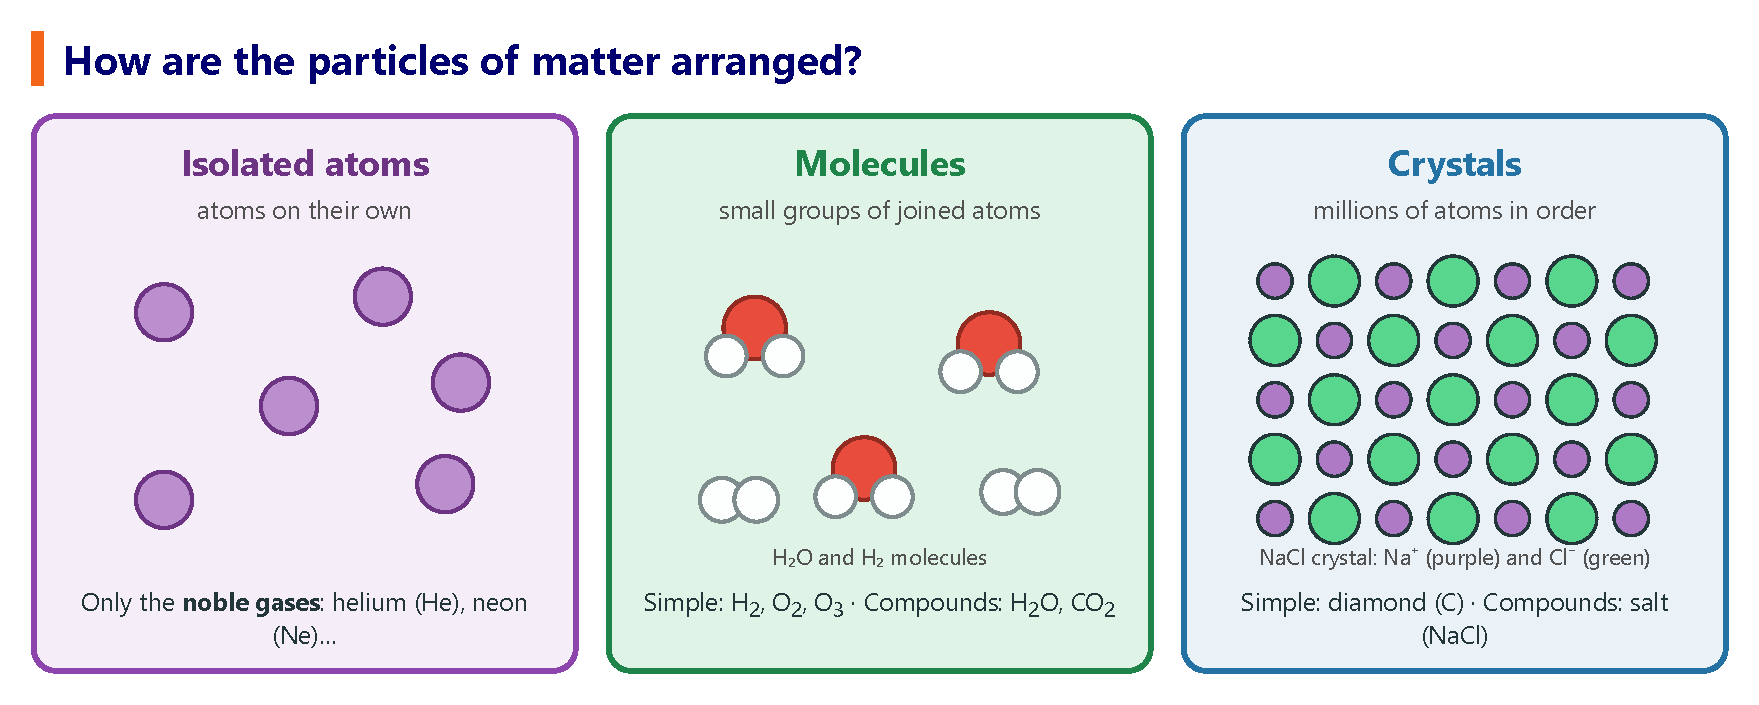
\includegraphics[width=\textwidth]{FigurasSVG/Unit_3_Diversity_of_Matter/pdf/particle_arrangements.pdf}
    \caption{The three ways in which the particles of a substance can be arranged.}
    \label{fig:u3_particle_arrangements}
\end{figure}

\begin{impt}
    \negsubro{Mixture vs.\ compound}: hydrogen gas (\ch{H2}) and oxygen gas (\ch{O2}) can be mixed in \textbf{any} proportion: that is a mixture. In water (\ch{H2O}) there are \textbf{always} 2 hydrogen atoms for each oxygen atom: that is a compound, and its properties are completely different from those of the two gases.
\end{impt}

\begin{exercise}
    Look at the three boxes in the figure below.
    \begin{figure}[H]
        \centering
        % [FIGURA ORIGINAL] \includegraphics[width=0.95\textwidth]{Unit_3/substances_particles}
        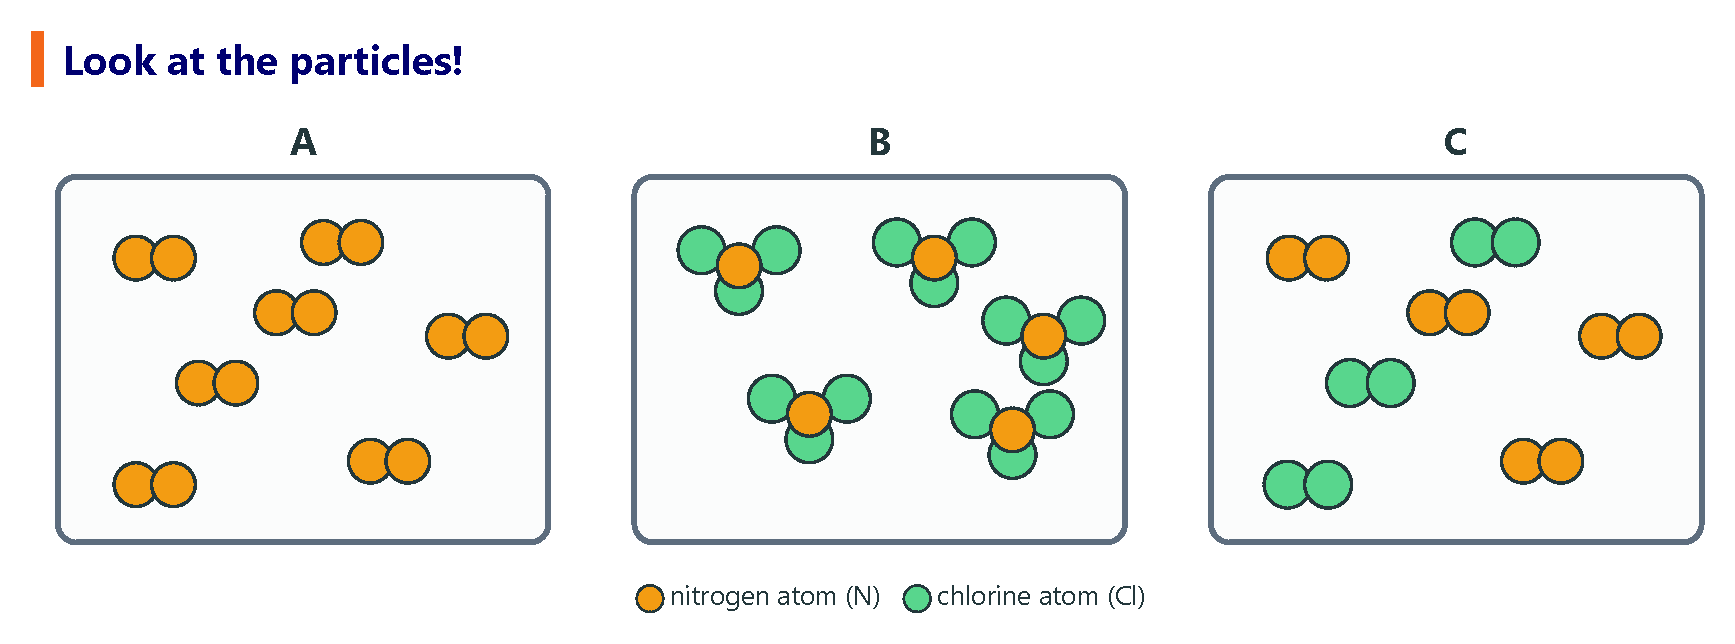
\includegraphics[width=0.95\textwidth]{FigurasSVG/Unit_3_Diversity_of_Matter/pdf/substances_particles.pdf}
    \end{figure}
    Which box shows: a) a simple substance; b) a compound; c) a mixture? Explain how you know.
    \begin{solu}
        \begin{enumerate}[label=\alph*)]
            \item \textbf{A}: all the molecules are identical (\ch{N2}) and made of only one type of atom.
            \item \textbf{B}: all the molecules are identical (\ch{NCl3}), but each one has two types of atom.
            \item \textbf{C}: there are two different types of molecules (\ch{N2} and \ch{Cl2}).
        \end{enumerate}
    \end{solu}
\end{exercise}

\begin{exercise}
    Classify as a simple substance or a compound, and as made of molecules or a crystal: diamond (\ch{C}), sodium chloride (\ch{NaCl}), hydrogen gas (\ch{H2}), water (\ch{H2O}).
    \begin{solu}
        Diamond: simple substance, crystal. \\
        Sodium chloride: compound, crystal. \\
        Hydrogen gas: simple substance, molecules. \\
        Water: compound, molecules.
    \end{solu}
\end{exercise}

\begin{exercise}
    State whether each of these is made up of \textbf{isolated atoms}, \textbf{molecules} or a \textbf{crystal}: neon gas (\ch{Ne}); carbon dioxide gas (\ch{CO2}); a diamond (\ch{C}); common salt (\ch{NaCl}).
    \begin{solu}
        Neon: \textbf{isolated atoms} (noble gas). Carbon dioxide: \textbf{molecules}. Diamond: \textbf{crystal}. Common salt: \textbf{crystal}.
    \end{solu}
\end{exercise}

%----------------------------------------------------------------------------------------

\section{The periodic table of elements}

\begin{definition}[Periodic table]
    A table with the 118 known elements, in order of increasing \textbf{atomic number} \(Z\). The rows are called \negsubro{periods} (7) and the columns \negsubro{groups} (18).
\end{definition}

\begin{figure}[H]
    \centering
    % [FIGURA ORIGINAL] \includegraphics[width=\textwidth]{Unit_3/periodic_table}
    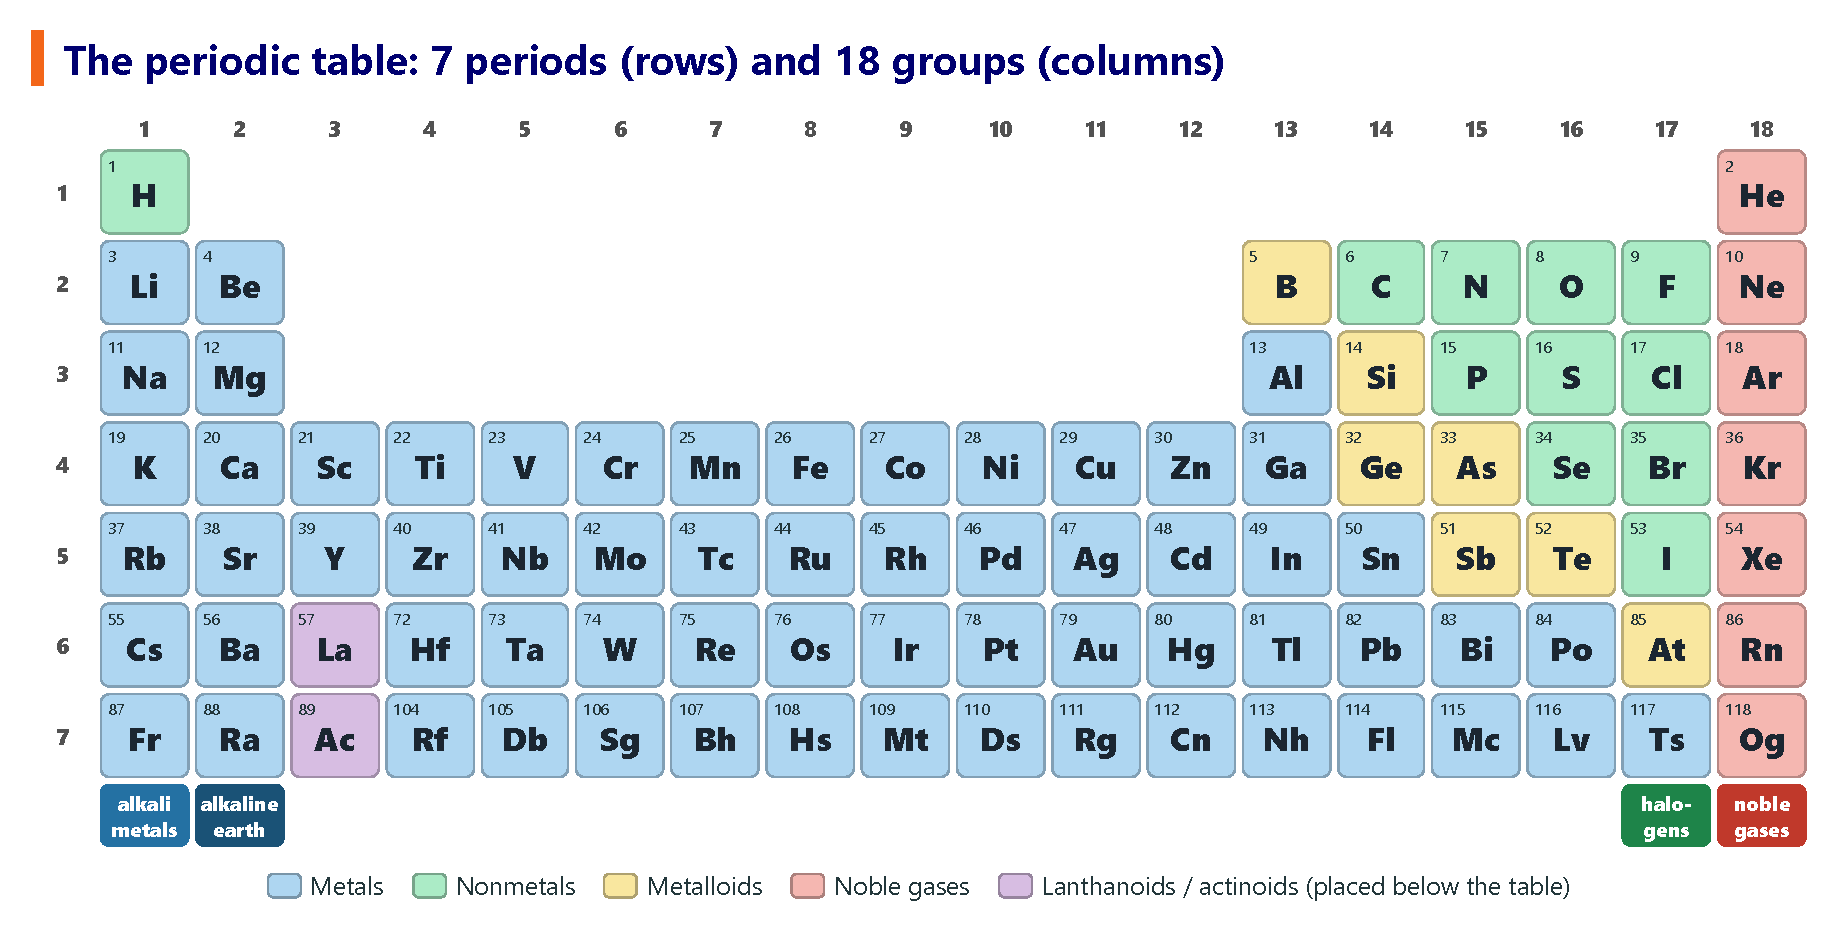
\includegraphics[width=\textwidth]{FigurasSVG/Unit_3_Diversity_of_Matter/pdf/periodic_table.pdf}
    \caption{The periodic table: metals, nonmetals, metalloids and noble gases.}
    \label{fig:u3_periodic_table}
\end{figure}

\begin{impt}
    \begin{itemize}
        \item Each element has a \textbf{symbol}: the first letter is always a capital, the second (if there is one) is lower case: \ch{H}, \ch{Ca}, \ch{Cl}.
        \item Elements in the same \textbf{group} have \textbf{similar properties}.
        \item The \textbf{period} number tells us how many electron shells the atoms have.
    \end{itemize}
\end{impt}

\begin{table}[H]
    \centering
    \small
    \renewcommand{\arraystretch}{1.35}
    \begin{tabular}{lp{9.5cm}}
        \toprule
        \textbf{Type} & \textbf{Properties} \\
        \midrule
        Metals & Most elements. Shiny, solid at room temperature (except mercury), good conductors of heat and electricity. \\
        Nonmetals & Poor conductors; many are gases (\ch{O2}, \ch{N2}) or brittle solids (\ch{S}, \ch{C}). \\
        Metalloids & Intermediate properties (silicon, used in computer chips). \\
        Noble gases & Group 18. Very stable: they almost never react. \\
        \bottomrule
    \end{tabular}
    \caption{Types of elements in the periodic table.}
    \label{tab:u3_element_types}
\end{table}

\begin{didyouknow}
    Dmitri Mendeleev organised the first periodic table in 1869. He left empty gaps for elements that nobody had discovered yet, and even predicted their properties. Years later, gallium and germanium were discovered\ldots{} and they fitted perfectly!
\end{didyouknow}

\begin{exercise}
    Use the periodic table to give the name and symbol of: the element with atomic number 6; the element with atomic number 17; the noble gas in period 2.
    \begin{solu}
        \(Z = 6\): \textbf{carbon}, \ch{C}. \quad \(Z = 17\): \textbf{chlorine}, \ch{Cl}. \quad Noble gas in period 2: \textbf{neon}, \ch{Ne}.
    \end{solu}
\end{exercise}

\begin{exercise}
    Say whether each element is a metal, a nonmetal, a metalloid or a noble gas: sodium (\ch{Na}), oxygen (\ch{O}), silicon (\ch{Si}), argon (\ch{Ar}), iron (\ch{Fe}).
    \begin{solu}
        Sodium: metal. Oxygen: nonmetal. Silicon: metalloid. Argon: noble gas. Iron: metal.
    \end{solu}
\end{exercise}

\begin{exercise}
    Elements X, Y and Z are in the same \textbf{period}, but in different groups. What does this tell you about the number of electron shells in their atoms? Are they the same element?
    \begin{solu}
        They have the \textbf{same number of electron shells} (equal to the period number). They are \textbf{not} the same element: being in different groups, they have different atomic numbers.
    \end{solu}
\end{exercise}

\subsection{Some important groups}

\begin{table}[H]
    \centering
    \small
    \renewcommand{\arraystretch}{1.35}
    \begin{tabular}{lcp{7.5cm}}
        \toprule
        \textbf{Name} & \textbf{Group} & \textbf{Examples and properties} \\
        \midrule
        Alkali metals & 1 & \ch{Li}, \ch{Na}, \ch{K}: very reactive metals (they react violently with water). \\
        Alkaline earth metals & 2 & \ch{Mg}, \ch{Ca}: reactive metals. \\
        Halogens & 17 & \ch{F}, \ch{Cl}, \ch{Br}, \ch{I}: very reactive nonmetals. \\
        Noble gases & 18 & \ch{He}, \ch{Ne}, \ch{Ar}: very unreactive gases. \\
        \bottomrule
    \end{tabular}
    \caption{Some important groups of the periodic table.}
    \label{tab:u3_groups}
\end{table}

\begin{exercise}
    Name the group to which each element belongs, and say whether it is likely to be very reactive or very unreactive: potassium (\ch{K}), neon (\ch{Ne}), chlorine (\ch{Cl}).
    \begin{solu}
        Potassium: \textbf{alkali metal} (group 1), very reactive. \\
        Neon: \textbf{noble gas} (group 18), very unreactive. \\
        Chlorine: \textbf{halogen} (group 17), very reactive.
    \end{solu}
\end{exercise}

\begin{exercise}
    Sodium (\ch{Na}) and potassium (\ch{K}) both belong to group 1. Predict whether they react with water in a similar way, and explain why.
    \begin{solu}
        Yes. Elements in the same group have similar chemical properties. Both are \textbf{alkali metals}, so both react vigorously with water, producing hydrogen gas and a metal hydroxide.
    \end{solu}
\end{exercise}

\begin{exercise}
    Classify each element as an alkali metal, alkaline earth metal, halogen or noble gas: lithium (\ch{Li}), fluorine (\ch{F}), calcium (\ch{Ca}), krypton (\ch{Kr}), bromine (\ch{Br}).
    \begin{solu}
        Lithium: alkali metal. Fluorine: halogen. Calcium: alkaline earth metal. Krypton: noble gas. Bromine: halogen.
    \end{solu}
\end{exercise}

%----------------------------------------------------------------------------------------
%
%\section{How chemical compounds are named}
%
%\subsection{Binary compounds}
%
%\begin{definition}[Binary compound]
%    A compound made of atoms of \textbf{two} different elements (for example, oxides: oxygen + another element).
%\end{definition}
%
%\begin{figure}[H]
%    \centering
%    \includegraphics[width=\textwidth]{Unit_3/naming}
%    \caption{Naming compounds with prefixes.}
%    \label{fig:u3_naming}
%\end{figure}
%
%\begin{impt}
%    \negsubro{Rules}:
%    \begin{enumerate}[label=\numberballmDarkTeal]
%        \item In the \textbf{formula}, the element further to the right in the periodic table goes on the right (oxygen and the halogens usually go last).
%        \item In the \textbf{name}, we say the prefix + the \textbf{second} element ending in \textit{-ide}, and then the prefix + the first element.
%        \item The prefix \textit{mono-} is not used for the first element: \ch{CO} is carbon \textbf{mon}oxide, not monocarbon monoxide.
%    \end{enumerate}
%\end{impt}
%
%\begin{example}
%    \ch{CO2} \(\to\) \textbf{carbon dioxide}. \quad \ch{AlF3} \(\to\) \textbf{aluminium trifluoride}. \quad \ch{MgS} \(\to\) \textbf{magnesium sulphide}. \quad \ch{CCl4} \(\to\) \textbf{carbon tetrachloride}.
%\end{example}
%
%\begin{exercise}
%    Write the formula of: a) dinitrogen pentoxide; b) silicon dioxide; c) hydrogen chloride.
%    \begin{solu}
%        a) \ch{N2O5}; \quad b) \ch{SiO2}; \quad c) \ch{HCl}.
%    \end{solu}
%\end{exercise}
%
%\begin{exercise}
%    Name these binary compounds: a) \ch{N2O3}; b) \ch{PCl5}; c) \ch{SO2}.
%    \begin{solu}
%        a) Dinitrogen trioxide; \quad b) phosphorus pentachloride; \quad c) sulphur dioxide.
%    \end{solu}
%\end{exercise}
%
%\begin{exercise}
%    Write the formula of: a) tetraphosphorus decaoxide; b) boron trifluoride; c) diiodine pentoxide.
%    \begin{solu}
%        a) \ch{P4O10}; \quad b) \ch{BF3}; \quad c) \ch{I2O5}.
%    \end{solu}
%\end{exercise}
%
%\subsection{Monatomic ions}
%
%\begin{definition}[Ion]
%    An atom that has gained or lost electrons, and so has an electric charge. A \negsubro{cation} is positive (it has \textbf{lost} electrons); an \negsubro{anion} is negative (it has \textbf{gained} electrons).
%\end{definition}
%
%\begin{figure}[H]
%    \centering
%    \includegraphics[width=\textwidth]{Unit_3/ions}
%    \caption{Sodium loses an electron (cation); chlorine gains one (anion).}
%    \label{fig:u3_ions}
%\end{figure}
%
%\begin{impt}
%    \textbf{Metals} tend to form cations (\ch{Na+}, \ch{Ca^2+}, \ch{Al^3+}); \textbf{nonmetals} tend to form anions (\ch{Cl-}, \ch{O^2-}, \ch{N^3-}). \newline
%    Naming: cations \(\to\) ``element + ion'' (\ch{Na+}: sodium ion); anions \(\to\) ending \textit{-ide} (\ch{Cl-}: chloride ion; \ch{O^2-}: oxide ion).
%\end{impt}
%
%\begin{example}
%    When sodium reacts with chlorine, each sodium atom \textbf{gives} one electron to a chlorine atom. \ch{Na+} and \ch{Cl-} are formed, and they attract each other, building the crystal of sodium chloride, \ch{NaCl} (table salt).
%\end{example}
%
%\begin{exercise}
%    Say whether each ion is a cation or an anion, and whether it comes from a metal or a nonmetal: \ch{K+}, \ch{S^2-}, \ch{Mg^2+}, \ch{F-}.
%    \begin{solu}
%        \ch{K+}: cation, metal. \quad \ch{S^2-}: anion, nonmetal. \quad \ch{Mg^2+}: cation, metal. \quad \ch{F-}: anion, nonmetal.
%    \end{solu}
%\end{exercise}
%
%\begin{exercise}
%    Write the formula of the ion formed, and say whether it is a cation or an anion: a) an aluminium atom that loses 3 electrons; b) a sulphur atom that gains 2 electrons; c) a calcium atom that loses 2 electrons.
%    \begin{solu}
%        a) \ch{Al^3+}, cation; \quad b) \ch{S^2-}, anion; \quad c) \ch{Ca^2+}, cation.
%    \end{solu}
%\end{exercise}
%
%\begin{exercise}
%    Name these ions: \ch{Na+}, \ch{Br-}, \ch{Mg^2+}, \ch{N^3-}.
%    \begin{solu}
%        Sodium ion; bromide ion; magnesium ion; nitride ion.
%    \end{solu}
%\end{exercise}
%
%\subsection{Compounds with three elements: hydroxides}
%
%\begin{definition}[Hydroxide]
%    A compound made of a \textbf{metal} and one or more \ch{OH} groups. It is named with a prefix that counts the \ch{OH} groups + \textit{hydroxide}.
%\end{definition}
%
%\begin{example}
%    \ch{NaOH} \(\to\) \textbf{sodium hydroxide}. \quad \ch{Fe(OH)2} \(\to\) \textbf{iron dihydroxide}. \quad \ch{Al(OH)3} \(\to\) \textbf{aluminium trihydroxide}.
%\end{example}
%
%\begin{exercise}
%    Write the formula of: a) magnesium dichloride; b) sulphur trioxide; c) calcium oxide.
%    \begin{solu}
%        a) \ch{MgCl2}; \quad b) \ch{SO3}; \quad c) \ch{CaO}.
%    \end{solu}
%\end{exercise}
%
%\begin{exercise}
%    Write the name of: a) \ch{MgCl2}; b) \ch{CO}; c) \ch{Na3N}; d) \ch{Al2O3}.
%    \begin{solu}
%        a) Magnesium dichloride; \quad b) carbon monoxide; \quad c) trisodium nitride; \quad d) dialuminium trioxide.
%    \end{solu}
%\end{exercise}
%
%\begin{exercise}
%    Write the name of \ch{Ca(OH)2} and the formula of iron trihydroxide.
%    \begin{solu}
%        \ch{Ca(OH)2} \(\to\) calcium dihydroxide. \quad Iron trihydroxide \(\to\) \ch{Fe(OH)3}.
%    \end{solu}
%\end{exercise}
%
%\begin{exercise}
%    Write the formula of potassium hydroxide and the name of \ch{Cu(OH)2}.
%    \begin{solu}
%        Potassium hydroxide \(\to\) \ch{KOH}. \quad \ch{Cu(OH)2} \(\to\) copper dihydroxide.
%    \end{solu}
%\end{exercise}
%
%\begin{exercise}
%    Write the formula of zinc dihydroxide, and give the name of \ch{Ba(OH)2}.
%    \begin{solu}
%        Zinc dihydroxide \(\to\) \ch{Zn(OH)2}. \quad \ch{Ba(OH)2} \(\to\) barium dihydroxide.
%    \end{solu}
%\end{exercise}

%----------------------------------------------------------------------------------------

\section*{Summary}

\begin{itemize}
    \item \textbf{Pure substances}: simple substances (one type of atom) or compounds (two or more types). \textbf{Mixtures}: homogeneous or heterogeneous.
    \item \textbf{Solutions}: homogeneous mixtures of a solvent (largest amount) and one or more solutes; dilute, concentrated or saturated. Alloys are solid solutions.
    \item \textbf{Concentration}: \(C = \text{mass of solute}/\text{volume of solution}\) (g/L) or \% mass. \textbf{Solubility}: the maximum amount of solute that can dissolve; for solids it usually increases with temperature, for gases it decreases.
    \item \textbf{Colloids}: look homogeneous but are heterogeneous; they show the Tyndall effect. \textbf{Emulsions}: colloids of two liquids that do not mix, stabilised by an emulsifier.
    \item \textbf{Atomic models}: Dalton, Thomson, Rutherford and Bohr.
    \item \textbf{The atom}: protons (+) and neutrons in the nucleus; electrons (\(-\)) in shells. \(Z\) = protons, \(A\) = protons + neutrons, \(N = A - Z\). \textbf{Isotopes}: same \(Z\), different \(A\).
    \item \textbf{Particles}: isolated atoms (noble gases), molecules or crystals.
    \item \textbf{Periodic table}: 118 elements ordered by \(Z\), in 7 periods and 18 groups; metals, nonmetals, metalloids and noble gases; important groups: alkali metals, alkaline earth metals, halogens and noble gases.
    \item \textbf{Naming}: prefixes (mono-, di-, tri-\ldots) give the number of atoms; binary compounds end in \textit{-ide}; hydroxides have a metal and \ch{OH} groups.
    \item \textbf{Ions}: cations (+, lose electrons, metals) and anions (\(-\), gain electrons, nonmetals).
\end{itemize}

\section{Vocabulary}

\begin{vocabulary}[Pure substance]
    A single substance, made up of only one type of matter. \newline
    \textbf{Translation to Spanish}: Sustancia pura
\end{vocabulary}

\begin{vocabulary}[Mixture]
    Matter made up of two or more pure substances. \newline
    \textbf{Translation to Spanish}: Mezcla
\end{vocabulary}

\begin{vocabulary}[Solution]
    A homogeneous mixture of a solvent and one or more solutes. \newline
    \textbf{Translation to Spanish}: Disolución
\end{vocabulary}

\begin{vocabulary}[Solute]
    The component of a solution found in the lowest proportion. \newline
    \textbf{Translation to Spanish}: Soluto
\end{vocabulary}

\begin{vocabulary}[Solvent]
    The component of a solution found in the highest proportion. \newline
    \textbf{Translation to Spanish}: Disolvente
\end{vocabulary}

\begin{vocabulary}[Alloy]
    A solid solution made up of two or more metals, or a metal and another substance. \newline
    \textbf{Translation to Spanish}: Aleación
\end{vocabulary}

\begin{vocabulary}[Concentration]
    The amount of solute dissolved in a given amount of solution. \newline
    \textbf{Translation to Spanish}: Concentración
\end{vocabulary}

\begin{vocabulary}[Solubility]
    The maximum amount of solute that can dissolve in a fixed amount of solvent, at a given temperature. \newline
    \textbf{Translation to Spanish}: Solubilidad
\end{vocabulary}

\begin{vocabulary}[Colloid]
    A heterogeneous mixture that has a homogeneous appearance. \newline
    \textbf{Translation to Spanish}: Coloide
\end{vocabulary}

\begin{vocabulary}[Emulsion]
    A colloid formed by two immiscible liquids stabilised with an emulsifier. \newline
    \textbf{Translation to Spanish}: Emulsión
\end{vocabulary}

\begin{vocabulary}[Atom]
    The smallest particle that makes up matter, according to atomic theory. \newline
    \textbf{Translation to Spanish}: Átomo
\end{vocabulary}

\begin{vocabulary}[Chemical element]
    A set of atoms that all have the same number of protons. \newline
    \textbf{Translation to Spanish}: Elemento químico
\end{vocabulary}

\begin{vocabulary}[Proton]
    A positively charged particle found in the nucleus of an atom. \newline
    \textbf{Translation to Spanish}: Protón
\end{vocabulary}

\begin{vocabulary}[Neutron]
    An uncharged particle found in the nucleus of an atom. \newline
    \textbf{Translation to Spanish}: Neutrón
\end{vocabulary}

\begin{vocabulary}[Electron]
    A negatively charged particle that orbits the nucleus of an atom. \newline
    \textbf{Translation to Spanish}: Electrón
\end{vocabulary}

\begin{vocabulary}[Isotope]
    An atom of a chemical element with a different number of neutrons from other atoms of the same element. \newline
    \textbf{Translation to Spanish}: Isótopo
\end{vocabulary}

\begin{vocabulary}[Tyndall effect]
    The scattering of light by the particles of a colloid, which makes a light beam visible inside it. \newline
    \textbf{Translation to Spanish}: Efecto Tyndall
\end{vocabulary}

\begin{vocabulary}[Saturated solution]
    A solution that contains the maximum amount of solute that can dissolve at that temperature. \newline
    \textbf{Translation to Spanish}: Disolución saturada
\end{vocabulary}

\begin{vocabulary}[Emulsifier]
    A substance that keeps two liquids that do not mix (such as oil and water) together. \newline
    \textbf{Translation to Spanish}: Emulsionante
\end{vocabulary}

\begin{vocabulary}[Atomic number]
    The number of protons in the nucleus of an atom (Z). \newline
    \textbf{Translation to Spanish}: Número atómico
\end{vocabulary}

\begin{vocabulary}[Mass number]
    The number of protons plus neutrons in the nucleus of an atom (A). \newline
    \textbf{Translation to Spanish}: Número másico
\end{vocabulary}

\begin{vocabulary}[Molecule]
    A specific, fixed group of atoms joined together. \newline
    \textbf{Translation to Spanish}: Molécula
\end{vocabulary}

\begin{vocabulary}[Periodic table]
    The table where all known chemical elements are arranged in order of atomic number. \newline
    \textbf{Translation to Spanish}: Tabla periódica
\end{vocabulary}

\begin{vocabulary}[Group]
    A column of the periodic table; elements in the same group have similar properties. \newline
    \textbf{Translation to Spanish}: Grupo
\end{vocabulary}

\begin{vocabulary}[Period]
    A row of the periodic table. \newline
    \textbf{Translation to Spanish}: Periodo
\end{vocabulary}

\begin{vocabulary}[Binary compound]
    A compound formed by atoms of two different chemical elements. \newline
    \textbf{Translation to Spanish}: Compuesto binario
\end{vocabulary}

\begin{vocabulary}[Ion]
    An atom, or group of atoms, that has gained or lost electrons and therefore has an electric charge. \newline
    \textbf{Translation to Spanish}: Ion
\end{vocabulary}

\begin{vocabulary}[Cation]
    A positively charged ion, formed when an atom loses electrons. \newline
    \textbf{Translation to Spanish}: Catión
\end{vocabulary}

\begin{vocabulary}[Anion]
    A negatively charged ion, formed when an atom gains electrons. \newline
    \textbf{Translation to Spanish}: Anión
\end{vocabulary}

\begin{vocabulary}[Hydroxide]
    A compound formed by a metal bound to one or more hydroxyl groups. \newline
    \textbf{Translation to Spanish}: Hidróxido
\end{vocabulary}



%------------------------------------------------


    \chapterimage{images/portada_cabeceras/cabecera_Unit4}
    \chapter{Nomenclature}
    % Unidad 4. Nomenclature (versión bilingüe: explicación en español; reglas en dos columnas,
% español a la izquierda e inglés a la derecha; ejemplos y ejercicios en los dos idiomas).
% Procede de src/Formulacion/inorganica/inorganica_nuevo_2_ESO.tex (sin preámbulo, portada ni soluciones propias:
% las soluciones van al fichero común del libro).
% Figuras: FigurasSVG/Unit_4_Nomenclature/pdf (generadas desde html/figuras_inorganica.html con
% html/exportar_figuras.py; las inglesas llevan el sufijo -en).
%
% Saberes básicos (LOMLOE) asociados a esta unidad
%
% Bloque B. La materia
%   - Nomenclatura: participación de un lenguaje científico común y universal formulando y nombrando
%     sustancias simples, iones monoatómicos y compuestos binarios mediante las reglas de nomenclatura de la IUPAC.
%     Justificación: toda la unidad trabaja la nomenclatura con prefijos multiplicadores (IUPAC 2005)
%     de óxidos, hidruros, compuestos de hidrógeno con no metales, sales binarias e hidróxidos,
%     en español y en inglés.

% --- Comandos propios de esta unidad ---
% Esquema de una regla de nomenclatura (figura vectorial generada desde HTML)
\newcommand{\esquemafig}[2][0.85]{\begin{center}\includegraphics[width=#1\textwidth]{FigurasSVG/Unit_4_Nomenclature/pdf/#2.pdf}\end{center}}
% Cabecera de los apartados "¿Cómo se formulan / nombran?"
\newcommand{\formulan}{\vspace*{2mm}\noindent\xmybox{\bfseries ¿Cómo se formulan? / \textit{From name to formula}}\par\smallskip}
\newcommand{\nombran}{\vspace*{2mm}\noindent\xmybox{\bfseries ¿Cómo se nombran? / \textit{How are they named?}}\par\smallskip}
\newcommand{\ejemplos}{\par\noindent\textbf{\uline{Ejemplos / \textit{Examples}}}:\par}
% Nombre incorrecto (tachado en rojo)
\newcommand{\mal}[1]{\textcolor{red}{\sout{#1}}}
% Texto en inglés dentro de una frase en español
\newcommand{\en}[1]{\textit{#1}}
% Figura generada desde HTML (sin figure[H]: tras las columnas de paracol, [H] puede salirse por el pie de la página)
\newcommand{\figura}[2][0.95]{\par\begin{center}\includegraphics[width=#1\textwidth]{FigurasSVG/Unit_4_Nomenclature/pdf/#2.pdf}\end{center}}
% Reglas en dos columnas: español a la izquierda, inglés a la derecha (\ingles cambia de columna)
\newcommand{\cabcol}[1]{\raggedright\noindent{\sffamily\bfseries\color{ocre}#1}\par\smallskip}
\newenvironment{reglas}{%
    \par\medskip\setlength{\columnseprule}{0.4pt}%
    \begin{paracol}{2}\cabcol{Español}%
}{%
    \end{paracol}\medskip%
}
\newcommand{\ingles}{\switchcolumn\cabcol{English}}

\spacing{1.3}
\raggedbottom % pages with large figures end where the text ends (no stretched gaps between boxes)

%=====================================================================
\section{¿Qué vamos a aprender?}
%=====================================================================

Cada sustancia química tiene un \negrita{nombre} y una \negrita{fórmula}. En este tema aprenderás a pasar de uno a otro, en español y en inglés:

\begin{itemize}
    \item \negrita{Formular} (\en{write the formula}): del nombre a la fórmula. \quad trióxido de dihierro / \en{diiron trioxide} \(\to\) \ch{Fe2O3}
    \item \negrita{Nombrar} (\en{name}): de la fórmula al nombre. \quad \ch{CO2} \(\to\) dióxido de carbono / \en{carbon dioxide}
\end{itemize}

Seguiremos las normas internacionales de la \negrita{IUPAC}. En este curso solo usaremos una forma de nombrar: la de los \negrita{prefijos}.

\begin{marker}
    \negrita{La fórmula es la misma en todos los idiomas}: \ch{CO2} es \ch{CO2} en español, en inglés o en chino. Lo que cambia es el \negrita{nombre}, y en inglés las palabras van en \negrita{otro orden}: dióxido de carbono \(\leftrightarrow\) \en{carbon dioxide}.
\end{marker}

\figura{fig2-formula}

\begin{exercise}
    ¿Cuántos átomos de cada elemento hay? / \en{How many atoms of each element are there?} \textbf{a)} \ch{H2O}; \textbf{b)} \ch{CO2}; \textbf{c)} \ch{NH3}; \textbf{d)} \ch{Fe2O3}; \textbf{e)} \ch{CH4}; \textbf{f)} \ch{Al2S3}.
    \begin{solu}
        \textcolor{blue}{El subíndice indica el número de átomos; si no hay número, hay 1.}\\
        \textbf{a)} \textcolor{red}{2 H y 1 O}; \textbf{b)} \textcolor{red}{1 C y 2 O}; \textbf{c)} \textcolor{red}{1 N y 3 H}; \textbf{d)} \textcolor{red}{2 Fe y 3 O}; \textbf{e)} \textcolor{red}{1 C y 4 H}; \textbf{f)} \textcolor{red}{2 Al y 3 S}
    \end{solu}
\end{exercise}

%=====================================================================
\section{Lo que necesitas antes de empezar}
%=====================================================================

\subsection{Los prefijos / \en{Prefixes}}

Los prefijos son \negrita{los mismos en español y en inglés}: mono, di, tri, tetra, penta, hexa, hepta…

\figura[0.85]{fig2-prefijos}

\subsubsection*{El prefijo mono- casi nunca se escribe / \en{The prefix mono- is hardly ever written}}

\begin{reglas}
    El prefijo \negrita{mono-} (1) \negrita{normalmente se omite}: si no hay prefijo, hay un solo átomo.
    \begin{enumerate}[label=\numberballgreen]
        \item El elemento que se nombra \negrita{al final} nunca lleva mono: \ch{NaCl} cloruro de sodio, no \mal{cloruro de monosodio}.
        \item El otro, normalmente tampoco: \ch{CaO} óxido de calcio.
        \item Se mantiene si los mismos dos elementos forman \negrita{varios compuestos}: \ch{CO} \negrita{monóxido} de carbono (existe el \ch{CO2}).
    \end{enumerate}
    \ingles
    The prefix \negrita{mono-} (1) is \negrita{usually left out}: if there is no prefix, there is only one atom.
    \begin{enumerate}[label=\numberballgreen]
        \item The element named \negrita{first} never takes mono: \ch{NaCl} sodium chloride, not \mal{monosodium chloride}.
        \item The other one usually does not either: \ch{CaO} calcium oxide.
        \item It is kept when the same two elements form \negrita{several compounds}: \ch{CO} carbon \negrita{monoxide} (\ch{CO2} also exists).
    \end{enumerate}
\end{reglas}

\begin{table}[H]
    \centering
    \caption{Casos más representativos en los que sí se escribe mono}
    \vspace{-5pt}
    \begin{tabular}{@{}clll@{}}
        \toprule
        \textbf{Fórmula} & \textbf{Nombre} & \textbf{\en{Name}} & \textbf{¿Por qué? / \en{Why?}} \\
        \midrule
        \ch{CO} & \negrita{monóxido} de carbono & \en{carbon \negrita{monoxide}} & existe / \en{there is} \ch{CO2} \\[3pt]
        \ch{NO} & \negrita{monóxido} de nitrógeno & \en{nitrogen \negrita{monoxide}} & existe / \en{there is} \ch{NO2} \\[3pt]
        \ch{N2O} & \negrita{monóxido} de dinitrógeno & \en{dinitrogen \negrita{monoxide}} & \ch{NO}, \ch{N2O3}, \ch{N2O5}… \\[3pt]
        \ch{FeO} & \negrita{monóxido} de hierro & \en{iron \negrita{monoxide}} & existe / \en{there is} \ch{Fe2O3} \\[3pt]
        \ch{FeS} & \negrita{mono}sulfuro de hierro & \en{iron \negrita{mono}sulfide} & existe / \en{there is} \ch{FeS2} \\
        \bottomrule
    \end{tabular}
    \label{tab:u4_mono}
\end{table}

\begin{marker}
    \negrita{mono + óxido = monóxido} y \en{\negrita{mono + oxide = monoxide}}: se pierde una o. Con los demás prefijos la IUPAC no quita ninguna vocal: di\negrita{ó}xido, penta\negrita{ó}xido / \en{penta\negrita{o}xide, tetra\negrita{o}xide}. En muchos libros en inglés verás también \en{pentoxide} o \en{tetroxide}: significan lo mismo.
\end{marker}

\begin{exercise}
    \textbf{1.} Escribe el prefijo / \en{Write the prefix}: \textbf{a)} 2; \textbf{b)} 3; \textbf{c)} 4; \textbf{d)} 5; \textbf{e)} 6; \textbf{f)} 7.\\
    \textbf{2.} ¿Qué número indica? / \en{Which number does it mean?} \textbf{a)} penta; \textbf{b)} hexa; \textbf{c)} di; \textbf{d)} tri.
    \begin{solu}
        \textcolor{blue}{Los prefijos son iguales en los dos idiomas.}\\
        \textbf{1. a)} \textcolor{red}{di}; \textbf{b)} \textcolor{red}{tri}; \textbf{c)} \textcolor{red}{tetra}; \textbf{d)} \textcolor{red}{penta}; \textbf{e)} \textcolor{red}{hexa}; \textbf{f)} \textcolor{red}{hepta}\\
        \textbf{2. a)} \textcolor{red}{5}; \textbf{b)} \textcolor{red}{6}; \textbf{c)} \textcolor{red}{2}; \textbf{d)} \textcolor{red}{3}
    \end{solu}
\end{exercise}

\begin{exercise}
    ¿Lleva mono o no? Nombra en español y en inglés / \en{Mono or not? Name in Spanish and in English}: \textbf{a)} \ch{CO}; \textbf{b)} \ch{KCl}; \textbf{c)} \ch{NO}; \textbf{d)} \ch{MgO}; \textbf{e)} \ch{N2O}; \textbf{f)} \ch{LiH}.
    \begin{solu}
        \textcolor{blue}{Mono solo se mantiene en los casos de la tabla.}\\
        \textbf{a)} \textcolor{red}{monóxido de carbono} · \textcolor{red}{\en{carbon monoxide}}; \textbf{b)} \textcolor{red}{cloruro de potasio} · \textcolor{red}{\en{potassium chloride}}; \textbf{c)} \textcolor{red}{monóxido de nitrógeno} · \textcolor{red}{\en{nitrogen monoxide}}; \textbf{d)} \textcolor{red}{óxido de magnesio} · \textcolor{red}{\en{magnesium oxide}}; \textbf{e)} \textcolor{red}{monóxido de dinitrógeno} · \textcolor{red}{\en{dinitrogen monoxide}}; \textbf{f)} \textcolor{red}{hidruro de litio} · \textcolor{red}{\en{lithium hydride}}
    \end{solu}
\end{exercise}

\subsection{¿Qué elemento se escribe a la derecha? / \en{Which element is written on the right?}}

La fórmula se escribe igual en los dos idiomas, así que esta regla también es la misma:

\begin{reglas}
    \begin{itemize}
        \item Los \negrita{metales} se escriben siempre a la \negrita{izquierda}.
        \item Entre dos no metales, el que está \negrita{más a la derecha} en la fila de abajo se escribe a la \negrita{derecha}.
    \end{itemize}
    \ingles
    \begin{itemize}
        \item \negrita{Metals} are always written on the \negrita{left}.
        \item Between two non-metals, the one \negrita{further to the right} in the row below is written on the \negrita{right}.
    \end{itemize}
\end{reglas}

\figura{fig-secuencia}

\ejemplos
\ballnumber{1} : Na y Cl \(\to\) \ch{NaCl} \quad \ballnumber{2} : C y O \(\to\) \ch{CO2} \quad \ballnumber{3} : N y H \(\to\) \ch{NH3} \quad \ballnumber{4} : H y Cl \(\to\) \ch{HCl}

\begin{exercise}
    ¿Qué elemento se escribe a la derecha? / \en{Which element is written on the right?} \textbf{a)} Na y Br; \textbf{b)} S y O; \textbf{c)} H y S; \textbf{d)} N y H; \textbf{e)} Cl y O; \textbf{f)} O y F.
    \begin{solu}
        \textbf{a)} \textcolor{red}{Br} (el Na es un metal); \textbf{b)} \textcolor{red}{O}; \textbf{c)} \textcolor{red}{S}; \textbf{d)} \textcolor{red}{H}; \textbf{e)} \textcolor{red}{Cl} (los halógenos van a la derecha del oxígeno); \textbf{f)} \textcolor{red}{F}
    \end{solu}
\end{exercise}

\subsection{Los nombres de los elementos en inglés / \en{Element names in English}}

Para nombrar en inglés necesitas saber cómo se llama cada elemento. Muchos se parecen al español (\en{sodium}, \en{calcium}, \en{carbon}), pero otros son muy distintos: \negrita{hierro} es \en{iron}, \negrita{plomo} es \en{lead}, \negrita{estaño} es \en{tin} y \negrita{azufre} es \en{sulfur}.

\begin{table}[H]
    \centering
    \caption{Nombres de los metales en español y en inglés}
    \vspace{-5pt}
    \begin{tabular}{@{}cll@{\hspace{1cm}}cll@{}}
        \toprule
        \textbf{Símbolo} & \textbf{Español} & \textbf{\en{English}} & \textbf{Símbolo} & \textbf{Español} & \textbf{\en{English}} \\
        \midrule
        Li & litio & \en{lithium} & Mn & manganeso & \en{manganese} \\[3pt]
        Na & sodio & \en{sodium} & Fe & hierro & \en{iron} \\[3pt]
        K & potasio & \en{potassium} & Co & cobalto & \en{cobalt} \\[3pt]
        Cs & cesio & \en{caesium} (EE.\,UU.: \en{cesium}) & Ni & níquel & \en{nickel} \\[3pt]
        Be & berilio & \en{beryllium} & Cu & cobre & \en{copper} \\[3pt]
        Mg & magnesio & \en{magnesium} & Ag & plata & \en{silver} \\[3pt]
        Ca & calcio & \en{calcium} & Au & oro & \en{gold} \\[3pt]
        Sr & estroncio & \en{strontium} & Zn & cinc & \en{zinc} \\[3pt]
        Ba & bario & \en{barium} & Cd & cadmio & \en{cadmium} \\[3pt]
        Al & aluminio & \en{aluminium} (EE.\,UU.: \en{aluminum}) & Hg & mercurio & \en{mercury} \\[3pt]
        Cr & cromo & \en{chromium} & Sn & estaño & \en{tin} \\[3pt]
        Pt & platino & \en{platinum} & Pb & plomo & \en{lead} \\
        \bottomrule
    \end{tabular}
    \label{tab:u4_metales_en}
\end{table}

\begin{table}[H]
    \centering
    \caption{Nombres de los no metales y su forma terminada en -uro / \en{-ide}}
    \vspace{-5pt}
    \begin{tabular}{@{}cllll@{}}
        \toprule
        \textbf{Símbolo} & \textbf{Español} & \textbf{\en{English}} & \textbf{-uro} & \textbf{\en{-ide}} \\
        \midrule
        H & hidrógeno & \en{hydrogen} & hidruro & \en{hydride} \\[3pt]
        O & oxígeno & \en{oxygen} & óxido & \en{oxide} \\[3pt]
        F & flúor & \en{fluorine} & fluoruro & \en{fluoride} \\[3pt]
        Cl & cloro & \en{chlorine} & cloruro & \en{chloride} \\[3pt]
        Br & bromo & \en{bromine} & bromuro & \en{bromide} \\[3pt]
        I & yodo & \en{iodine} & yoduro & \en{iodide} \\[3pt]
        S & azufre & \en{sulfur} (R.\,Unido: \en{sulphur}) & sulfuro & \en{sulfide} \\[3pt]
        Se & selenio & \en{selenium} & seleniuro & \en{selenide} \\[3pt]
        Te & teluro & \en{tellurium} & telururo & \en{telluride} \\[3pt]
        N & nitrógeno & \en{nitrogen} & nitruro & \en{nitride} \\[3pt]
        P & fósforo & \en{phosphorus} & fosfuro & \en{phosphide} \\[3pt]
        C & carbono & \en{carbon} & carburo & \en{carbide} \\[3pt]
        Si & silicio & \en{silicon} & siliciuro & \en{silicide} \\[3pt]
        B & boro & \en{boron} & boruro & \en{boride} \\[3pt]
        As & arsénico & \en{arsenic} & --- & --- \\[3pt]
        Sb & antimonio & \en{antimony} & --- & --- \\
        \bottomrule
    \end{tabular}
    \label{tab:u4_nometales_en}
\end{table}

\subsection{La raíz del nombre: -uro en español, \en{-ide} en inglés}

El elemento de la derecha se nombra con la \negrita{raíz} de su nombre seguida de una terminación: \negrita{-uro} en español y \negrita{\en{-ide}} en inglés. La forma de obtener la raíz es parecida, pero \negrita{en inglés se parte del nombre inglés del elemento}:

\begin{reglas}
    \begin{enumerate}[label=\numberballgreen]
        \item Escribe el nombre del elemento y \negrita{tacha la terminación}: clor\mal{o}, nitr\mal{ógeno}, carb\mal{ono}, fósf\mal{oro}.
        \item Lo que queda es la \negrita{raíz} (sin tilde): clor, nitr, carb, fosf.
        \item Añade \negrita{-uro}: cloruro, nitruro, carburo, fosfuro.
    \end{enumerate}
    Casos especiales: el \negrita{azufre} usa una raíz latina (\negrita{sulf}uro) y el \negrita{oxígeno} no lleva -uro: se dice \negrita{óxido}.
    \ingles
    \begin{enumerate}[label=\numberballgreen]
        \item Write the English name and \negrita{cross out the ending}: chlor\mal{ine}, nitr\mal{ogen}, carb\mal{on}, phosph\mal{orus}.
        \item What is left is the \negrita{root}: chlor, nitr, carb, phosph.
        \item Add \negrita{-ide}: chloride, nitride, carbide, phosphide.
    \end{enumerate}
    No exceptions here: sulf\mal{ur} \(\to\) \negrita{sulfide} and ox\mal{ygen} \(\to\) \negrita{oxide} follow the same rule.
\end{reglas}

Las terminaciones que se quitan en inglés son casi siempre \negrita{-ine} (halógenos), \negrita{-ogen}/\negrita{-ygen}, \negrita{-on}, \negrita{-orus}, \negrita{-ur} e \negrita{-ium}. Fíjate en que el oxígeno, que en español es una excepción (óxido), en inglés sigue la regla: \en{ox + ide = oxide}.

\figura{fig-raiz}

\figura{fig-raiz-en}

\figura[0.85]{fig2-uro}

\figura[0.85]{fig2-uro-en}

\begin{exercise}
    Escribe la raíz y el nombre terminado en -uro y en \en{-ide} / \en{Write the root and the name ending in -uro and in -ide}: \textbf{a)} cloro / \en{chlorine}; \textbf{b)} azufre / \en{sulfur}; \textbf{c)} nitrógeno / \en{nitrogen}; \textbf{d)} fósforo / \en{phosphorus}; \textbf{e)} bromo / \en{bromine}; \textbf{f)} carbono / \en{carbon}; \textbf{g)} oxígeno / \en{oxygen}; \textbf{h)} yodo / \en{iodine}.
    \begin{solu}
        \textbf{a)} clor \(\to\) \textcolor{red}{cloruro} · \en{chlor} \(\to\) \textcolor{red}{\en{chloride}}; \textbf{b)} sulf \(\to\) \textcolor{red}{sulfuro} · \en{sulf} \(\to\) \textcolor{red}{\en{sulfide}}; \textbf{c)} nitr \(\to\) \textcolor{red}{nitruro} · \en{nitr} \(\to\) \textcolor{red}{\en{nitride}}; \textbf{d)} fosf \(\to\) \textcolor{red}{fosfuro} · \en{phosph} \(\to\) \textcolor{red}{\en{phosphide}}; \textbf{e)} brom \(\to\) \textcolor{red}{bromuro} · \en{brom} \(\to\) \textcolor{red}{\en{bromide}}; \textbf{f)} carb \(\to\) \textcolor{red}{carburo} · \en{carb} \(\to\) \textcolor{red}{\en{carbide}}; \textbf{g)} \textcolor{red}{óxido} (excepción) · \en{ox} \(\to\) \textcolor{red}{\en{oxide}} (en inglés sigue la regla); \textbf{h)} yod \(\to\) \textcolor{red}{yoduro} · \en{iod} \(\to\) \textcolor{red}{\en{iodide}}
    \end{solu}
\end{exercise}

%=====================================================================
\section{La receta para nombrar y formular}
%=====================================================================

Todos los compuestos de este tema tienen \negrita{dos partes} y se nombran con la misma receta. Pero \negrita{el orden de las palabras cambia} de un idioma a otro.

\subsection{Nombrar: de la fórmula al nombre / \en{From formula to name}}

\begin{reglas}
    Se lee la fórmula de \negrita{derecha a izquierda}:
    \begin{enumerate}[label=\numberballgreen]
        \item Raíz del elemento de la \negrita{derecha} + \negrita{-uro} (si es el oxígeno, \negrita{óxido}), con el prefijo de su número de átomos delante.
        \item Escribe \negrita{de}.
        \item Prefijo del elemento de la \negrita{izquierda} (si solo hay 1, nada) y su nombre.
    \end{enumerate}
    \ch{Al2S3}: \negrita{tri}sulfuro \negrita{de} \negrita{di}aluminio
    \ingles
    Read the formula from \negrita{left to right}:
    \begin{enumerate}[label=\numberballgreen]
        \item Prefix for the element on the \negrita{left} (nothing if there is only 1) and its name.
        \item Prefix for the element on the \negrita{right} + its root + \negrita{-ide}.
        \item There is \negrita{no} word in between: never write \mal{of}.
    \end{enumerate}
    \ch{Al2S3}: \negrita{di}aluminium \negrita{tri}sulfide
\end{reglas}

\esquemafig{esq-binario}

\esquemafig{esq-binario-en}

\figura{fig-receta}

\figura{fig-receta-en}

\begin{marker}
    \negrita{La gran diferencia es el orden}. En español se nombra primero lo de la derecha y se une con \negrita{de}; en inglés se nombra en el mismo orden que la fórmula y no hay ninguna palabra en medio:
    \begin{center}
        \ch{NaCl}: cloruro \negrita{de} sodio \(\leftrightarrow\) \en{sodium chloride} \qquad \ch{CO2}: dióxido \negrita{de} carbono \(\leftrightarrow\) \en{carbon dioxide}
    \end{center}
\end{marker}

\subsection{Formular: del nombre a la fórmula / \en{From name to formula}}

\begin{reglas}
    \begin{enumerate}[label=\numberballgreen]
        \item Corta el nombre por \negrita{de}.
        \item Traduce los prefijos a números.
        \item Escribe \negrita{al revés}: primero lo que va después de «de».
    \end{enumerate}
    trióxido de dihierro \(\to\) \ch{Fe2O3}
    \ingles
    \begin{enumerate}[label=\numberballgreen]
        \item Split the name into its \negrita{two words}.
        \item Turn the prefixes into numbers.
        \item Write them \negrita{in the same order}: the first word goes on the left.
    \end{enumerate}
    diiron trioxide \(\to\) \ch{Fe2O3}
\end{reglas}

\figura{fig2-formular}

\figura{fig2-formular-en}

\begin{marker}
    \negrita{No simplifiques nunca / \en{Never simplify}.} La fórmula se escribe tal y como dice el nombre: tetraóxido de dinitrógeno / \en{dinitrogen tetraoxide} es \ch{N2O4} (no \mal{\ch{NO2}}, que es otra sustancia).
\end{marker}

\subsection{¿Qué tipo de compuesto es? / \en{What type of compound is it?}}

\figura{fig2-identificar}

\figura{fig2-identificar-en}

\begin{exercise}
    Indica de qué tipo es cada compuesto, en español y en inglés / \en{Say what type of compound it is, in Spanish and in English}: \textbf{a)} \ch{SO2}; \textbf{b)} \ch{KH}; \textbf{c)} \ch{KOH}; \textbf{d)} \ch{HBr}; \textbf{e)} \ch{KBr}; \textbf{f)} \ch{NH3}.
    \begin{solu}
        \textbf{a)} \textcolor{red}{óxido} · \textcolor{red}{\en{oxide}}; \textbf{b)} \textcolor{red}{hidruro} · \textcolor{red}{\en{hydride}}; \textbf{c)} \textcolor{red}{hidróxido} · \textcolor{red}{\en{hydroxide}}; \textbf{d)} \textcolor{red}{hidrógeno + no metal} · \textcolor{red}{\en{hydrogen + non-metal}} (bromuro de hidrógeno · \en{hydrogen bromide}); \textbf{e)} \textcolor{red}{sal binaria} · \textcolor{red}{\en{binary salt}} (bromuro de potasio · \en{potassium bromide}); \textbf{f)} \textcolor{red}{nombre especial}: amoniaco · \en{ammonia}
    \end{solu}
\end{exercise}

%=====================================================================
\section{Óxidos / \en{Oxides}}
%=====================================================================

\begin{reglas}
    \negrita{Óxido}: compuesto de \negrita{oxígeno} y otro elemento. El oxígeno se escribe a la \negrita{derecha}.
    \begin{enumerate}[label=\numberballgreen]
        \item Prefijo del nº de oxígenos + \negrita{óxido}.
        \item \negrita{de}.
        \item Prefijo del nº de átomos del otro elemento + su nombre.
    \end{enumerate}
    \ch{Fe2O3}: \negrita{tri}óxido de \negrita{di}hierro
    \ingles
    \negrita{Oxide}: a compound of \negrita{oxygen} and another element. Oxygen is written on the \negrita{right}.
    \begin{enumerate}[label=\numberballgreen]
        \item Prefix for the number of atoms of the element + its name.
        \item Prefix for the number of oxygens + \negrita{oxide}.
    \end{enumerate}
    \ch{Fe2O3}: \negrita{di}iron \negrita{tri}oxide
\end{reglas}

\nombran
\esquemafig{esq-oxido-pref}

\esquemafig{esq-oxido-pref-en}

\ejemplos
\begin{center}
    \begin{tabular}{@{}cll@{}}
        \toprule
        \textbf{Fórmula} & \textbf{Nombre} & \textbf{\en{Name}} \\
        \midrule
        \ch{CO} & monóxido de carbono & \en{carbon monoxide} \\[3pt]
        \ch{CO2} & dióxido de carbono & \en{carbon dioxide} \\[3pt]
        \ch{SO3} & trióxido de azufre & \en{sulfur trioxide} \\[3pt]
        \ch{Na2O} & óxido de disodio & \en{disodium oxide} \\[3pt]
        \ch{Fe2O3} & trióxido de dihierro & \en{diiron trioxide} \\[3pt]
        \ch{N2O5} & pentaóxido de dinitrógeno & \en{dinitrogen pentaoxide} \\[3pt]
        \ch{CaO} & óxido de calcio & \en{calcium oxide} \\
        \bottomrule
    \end{tabular}
\end{center}

\formulan
\ballnumber{1} : dióxido de azufre / \en{sulfur dioxide} \(\to\) 2 O y 1 S \(\to\) \ch{SO2}

\ballnumber{2} : óxido de disodio / \en{disodium oxide} \(\to\) 1 O y 2 Na \(\to\) \ch{Na2O}

\ballnumber{3} : pentaóxido de difósforo / \en{diphosphorus pentaoxide} \(\to\) 5 O y 2 P \(\to\) \ch{P2O5}

\begin{marker}
    \negrita{¡Cuidado con los halógenos! / \en{Watch out for the halogens!}} Con F, Cl, Br e I el oxígeno va a la \negrita{izquierda} y el halógeno se nombra con raíz + uro / \en{root + ide}: \ch{OF2} \negrita{difluoruro de oxígeno} / \en{\negrita{oxygen difluoride}}, \ch{OCl2} \negrita{dicloruro de oxígeno} / \en{\negrita{oxygen dichloride}}. No son óxidos: no escribas \mal{\ch{Cl2O}} ni digas \mal{óxido de dicloro} / \mal{\en{dichlorine oxide}}.
\end{marker}
\esquemafig{esq-halogenuro-oxigeno}

\esquemafig{esq-halogenuro-oxigeno-en}

\begin{exercise}
    Nombra en español y en inglés / \en{Name in Spanish and in English}: \textbf{a)} \ch{CO2}; \textbf{b)} \ch{SO2}; \textbf{c)} \ch{CaO}; \textbf{d)} \ch{K2O}; \textbf{e)} \ch{Al2O3}; \textbf{f)} \ch{N2O3}; \textbf{g)} \ch{PbO2}; \textbf{h)} \ch{SiO2}; \textbf{i)} \ch{OCl2}.
    \begin{solu}
        \textbf{a)} \textcolor{red}{dióxido de carbono} · \textcolor{red}{\en{carbon dioxide}}; \textbf{b)} \textcolor{red}{dióxido de azufre} · \textcolor{red}{\en{sulfur dioxide}}; \textbf{c)} \textcolor{red}{óxido de calcio} · \textcolor{red}{\en{calcium oxide}}; \textbf{d)} \textcolor{red}{óxido de dipotasio} · \textcolor{red}{\en{dipotassium oxide}}; \textbf{e)} \textcolor{red}{trióxido de dialuminio} · \textcolor{red}{\en{dialuminium trioxide}}; \textbf{f)} \textcolor{red}{trióxido de dinitrógeno} · \textcolor{red}{\en{dinitrogen trioxide}}; \textbf{g)} \textcolor{red}{dióxido de plomo} · \textcolor{red}{\en{lead dioxide}}; \textbf{h)} \textcolor{red}{dióxido de silicio} · \textcolor{red}{\en{silicon dioxide}}; \textbf{i)} \textcolor{red}{dicloruro de oxígeno} · \textcolor{red}{\en{oxygen dichloride}} (no es un óxido)
    \end{solu}
\end{exercise}

\begin{exercise}
    Formula / \en{Write the formula}: \textbf{a)} monóxido de carbono; \textbf{b)} \en{sulfur trioxide}; \textbf{c)} óxido de dilitio; \textbf{d)} \en{iron monoxide}; \textbf{e)} pentaóxido de dinitrógeno; \textbf{f)} \en{magnesium oxide}.
    \begin{solu}
        \textbf{a)} \textcolor{red}{\ch{CO}}; \textbf{b)} \textcolor{red}{\ch{SO3}}; \textbf{c)} \textcolor{red}{\ch{Li2O}}; \textbf{d)} \textcolor{red}{\ch{FeO}}; \textbf{e)} \textcolor{red}{\ch{N2O5}}; \textbf{f)} \textcolor{red}{\ch{MgO}}
    \end{solu}
\end{exercise}

%=====================================================================
\section{Hidruros: metal + hidrógeno / \en{Hydrides: metal + hydrogen}}
%=====================================================================

\begin{reglas}
    \negrita{Hidruro}: compuesto de un \negrita{metal} y \negrita{hidrógeno}. El hidrógeno se escribe a la \negrita{derecha}.
    \begin{enumerate}[label=\numberballgreen]
        \item Prefijo del nº de hidrógenos + \negrita{hidruro}.
        \item \negrita{de} + nombre del metal (sin prefijo: siempre hay un solo átomo).
    \end{enumerate}
    \ch{CoH3}: \negrita{tri}hidruro de cobalto
    \ingles
    \negrita{Hydride}: a compound of a \negrita{metal} and \negrita{hydrogen}. Hydrogen is written on the \negrita{right}.
    \begin{enumerate}[label=\numberballgreen]
        \item Name of the metal (no prefix: there is always one atom).
        \item Prefix for the number of hydrogens + \negrita{hydride}.
    \end{enumerate}
    \ch{CoH3}: cobalt \negrita{tri}hydride
\end{reglas}

\nombran
\esquemafig{esq-hidruro-pref}

\esquemafig{esq-hidruro-pref-en}

\ejemplos
\begin{center}
    \begin{tabular}{@{}cll@{}}
        \toprule
        \textbf{Fórmula} & \textbf{Nombre} & \textbf{\en{Name}} \\
        \midrule
        \ch{NaH} & hidruro de sodio & \en{sodium hydride} \\[3pt]
        \ch{CaH2} & dihidruro de calcio & \en{calcium dihydride} \\[3pt]
        \ch{AlH3} & trihidruro de aluminio & \en{aluminium trihydride} \\
        \bottomrule
    \end{tabular}
\end{center}

\formulan
\ballnumber{1} : dihidruro de hierro / \en{iron dihydride} \(\to\) 1 Fe y 2 H \(\to\) \ch{FeH2} \quad \ballnumber{2} : hidruro de litio / \en{lithium hydride} \(\to\) \ch{LiH}

\begin{exercise}
    \textbf{1.} Nombra en español y en inglés / \en{Name in Spanish and in English}: \textbf{a)} \ch{KH}; \textbf{b)} \ch{MgH2}; \textbf{c)} \ch{FeH3}; \textbf{d)} \ch{PbH4}; \textbf{e)} \ch{CuH}.\\
    \textbf{2.} Formula / \en{Write the formula}: \textbf{a)} hidruro de sodio; \textbf{b)} \en{barium dihydride}; \textbf{c)} trihidruro de cobalto; \textbf{d)} \en{tin tetrahydride}.
    \begin{solu}
        \textbf{1. a)} \textcolor{red}{hidruro de potasio} · \textcolor{red}{\en{potassium hydride}}; \textbf{b)} \textcolor{red}{dihidruro de magnesio} · \textcolor{red}{\en{magnesium dihydride}}; \textbf{c)} \textcolor{red}{trihidruro de hierro} · \textcolor{red}{\en{iron trihydride}}; \textbf{d)} \textcolor{red}{tetrahidruro de plomo} · \textcolor{red}{\en{lead tetrahydride}}; \textbf{e)} \textcolor{red}{hidruro de cobre} · \textcolor{red}{\en{copper hydride}}\\
        \textbf{2. a)} \textcolor{red}{\ch{NaH}}; \textbf{b)} \textcolor{red}{\ch{BaH2}}; \textbf{c)} \textcolor{red}{\ch{CoH3}}; \textbf{d)} \textcolor{red}{\ch{SnH4}}
    \end{solu}
\end{exercise}

%=====================================================================
\section{Hidrógeno + no metal / \en{Hydrogen + non-metal}}
%=====================================================================

\subsection{Con los grupos 16 (S, Se, Te) y 17 (F, Cl, Br, I): el hidrógeno va a la izquierda}

\begin{reglas}
    Con estos no metales el hidrógeno se escribe a la \negrita{izquierda}.
    \begin{enumerate}[label=\numberballgreen]
        \item Raíz del no metal + \negrita{-uro}.
        \item \negrita{de} + prefijo del nº de hidrógenos + \negrita{hidrógeno}.
    \end{enumerate}
    \ch{H2S}: sulfuro de \negrita{di}hidrógeno
    \ingles
    With these non-metals hydrogen is written on the \negrita{left}.
    \begin{enumerate}[label=\numberballgreen]
        \item Prefix for the number of hydrogens + \negrita{hydrogen}.
        \item Root of the non-metal + \negrita{-ide}.
    \end{enumerate}
    \ch{H2S}: \negrita{di}hydrogen sulfide
\end{reglas}

\esquemafig{esq-hidrogeno-nm}

\esquemafig{esq-hidrogeno-nm-en}

\ejemplos
\ballnumber{1} : \ch{HF}: fluoruro de hidrógeno / \en{hydrogen fluoride} \quad \ballnumber{2} : \ch{HCl}: cloruro de hidrógeno / \en{hydrogen chloride} \quad \ballnumber{3} : \ch{H2S}: sulfuro de dihidrógeno / \en{dihydrogen sulfide}

\begin{marker}
    \negrita{¿Y el «ácido clorhídrico» / \en{hydrochloric acid}?} Es el nombre tradicional de la mezcla de cloruro de hidrógeno (\ch{HCl}) con agua. No es un nombre de la IUPAC: el compuesto \ch{HCl} se llama siempre \negrita{cloruro de hidrógeno} / \en{\negrita{hydrogen chloride}}.
\end{marker}

\subsection{Tres nombres especiales: agua, amoniaco y metano / \en{water, ammonia and methane}}

Algunas sustancias muy conocidas tienen un \negrita{nombre propio} que la IUPAC acepta. Hay que aprenderlos de memoria, en los dos idiomas:

\begin{center}
    \begin{tabular}{@{}cccl@{}}
        \toprule
        \textbf{Fórmula} & \textbf{Nombre especial} & \textbf{\en{Special name}} & \textbf{Con prefijos / \en{With prefixes}} \\
        \midrule
        \ch{H2O} & \negrita{agua} & \en{\negrita{water}} & --- \\[3pt]
        \ch{NH3} & \negrita{amoniaco} & \en{\negrita{ammonia}} & trihidruro de nitrógeno / \en{nitrogen trihydride} \\[3pt]
        \ch{CH4} & \negrita{metano} & \en{\negrita{methane}} & tetrahidruro de carbono / \en{carbon tetrahydride} \\
        \bottomrule
    \end{tabular}
\end{center}

Fíjate: con el N y el C el hidrógeno va a la \negrita{derecha} (\ch{NH3}, \ch{CH4}).

\begin{exercise}
    \textbf{1.} Nombra en español y en inglés / \en{Name in Spanish and in English}: \textbf{a)} \ch{HBr}; \textbf{b)} \ch{HI}; \textbf{c)} \ch{H2S}; \textbf{d)} \ch{H2O}; \textbf{e)} \ch{NH3}; \textbf{f)} \ch{CH4}.\\
    \textbf{2.} Formula / \en{Write the formula}: \textbf{a)} cloruro de hidrógeno; \textbf{b)} \en{hydrogen fluoride}; \textbf{c)} sulfuro de dihidrógeno; \textbf{d)} \en{ammonia}; \textbf{e)} metano; \textbf{f)} \en{water}.
    \begin{solu}
        \textbf{1. a)} \textcolor{red}{bromuro de hidrógeno} · \textcolor{red}{\en{hydrogen bromide}}; \textbf{b)} \textcolor{red}{yoduro de hidrógeno} · \textcolor{red}{\en{hydrogen iodide}}; \textbf{c)} \textcolor{red}{sulfuro de dihidrógeno} · \textcolor{red}{\en{dihydrogen sulfide}}; \textbf{d)} \textcolor{red}{agua} · \textcolor{red}{\en{water}}; \textbf{e)} \textcolor{red}{amoniaco} · \textcolor{red}{\en{ammonia}}; \textbf{f)} \textcolor{red}{metano} · \textcolor{red}{\en{methane}}\\
        \textbf{2. a)} \textcolor{red}{\ch{HCl}}; \textbf{b)} \textcolor{red}{\ch{HF}}; \textbf{c)} \textcolor{red}{\ch{H2S}}; \textbf{d)} \textcolor{red}{\ch{NH3}}; \textbf{e)} \textcolor{red}{\ch{CH4}}; \textbf{f)} \textcolor{red}{\ch{H2O}}
    \end{solu}
\end{exercise}

%=====================================================================
\section{Sales binarias / \en{Binary salts}}
%=====================================================================

\begin{reglas}
    \negrita{Sal binaria}: dos elementos; el de la \negrita{derecha} es un no metal (pero no el O ni el H). El de la izquierda puede ser un metal o un no metal.
    \begin{enumerate}[label=\numberballgreen]
        \item Prefijo + raíz del no metal de la derecha + \negrita{-uro}.
        \item \negrita{de}.
        \item Prefijo + nombre del elemento de la izquierda.
    \end{enumerate}
    \ch{Ca3P2}: \negrita{di}fosfuro de \negrita{tri}calcio
    \ingles
    \negrita{Binary salt}: two elements; the one on the \negrita{right} is a non-metal (but not O or H). The one on the left can be a metal or a non-metal.
    \begin{enumerate}[label=\numberballgreen]
        \item Prefix + name of the element on the left.
        \item Prefix + root of the non-metal on the right + \negrita{-ide}.
    \end{enumerate}
    \ch{Ca3P2}: \negrita{tri}calcium \negrita{di}phosphide
\end{reglas}

\nombran
\esquemafig{esq-sal-pref}

\esquemafig{esq-sal-pref-en}

\ejemplos
\begin{center}
    \begin{tabular}{@{}cll@{}}
        \toprule
        \textbf{Fórmula} & \textbf{Nombre} & \textbf{\en{Name}} \\
        \midrule
        \multicolumn{3}{@{}l}{\textit{Metal + no metal / Metal + non-metal}} \\[3pt]
        \ch{NaCl} & cloruro de sodio & \en{sodium chloride} \\[3pt]
        \ch{CaF2} & difluoruro de calcio & \en{calcium difluoride} \\[3pt]
        \ch{FeS} & monosulfuro de hierro & \en{iron monosulfide} \\[3pt]
        \ch{Al2S3} & trisulfuro de dialuminio & \en{dialuminium trisulfide} \\[3pt]
        \multicolumn{3}{@{}l}{\textit{No metal + no metal / Non-metal + non-metal}} \\[3pt]
        \ch{PCl3} & tricloruro de fósforo & \en{phosphorus trichloride} \\[3pt]
        \ch{CCl4} & tetracloruro de carbono & \en{carbon tetrachloride} \\[3pt]
        \ch{SF6} & hexafluoruro de azufre & \en{sulfur hexafluoride} \\[3pt]
        \ch{CS2} & disulfuro de carbono & \en{carbon disulfide} \\
        \bottomrule
    \end{tabular}
\end{center}

\formulan
\ballnumber{1} : difosfuro de tricalcio / \en{tricalcium diphosphide} \(\to\) 3 Ca y 2 P \(\to\) \ch{Ca3P2} \quad \ballnumber{2} : pentacloruro de fósforo / \en{phosphorus pentachloride} \(\to\) \ch{PCl5}

\begin{exercise}
    \textbf{1.} Nombra en español y en inglés / \en{Name in Spanish and in English}: \textbf{a)} \ch{KCl}; \textbf{b)} \ch{MgBr2}; \textbf{c)} \ch{Na2S}; \textbf{d)} \ch{AgI}; \textbf{e)} \ch{FeCl3}; \textbf{f)} \ch{NCl3}; \textbf{g)} \ch{PBr5}.\\
    \textbf{2.} Formula / \en{Write the formula}: \textbf{a)} bromuro de sodio; \textbf{b)} \en{zinc dichloride}; \textbf{c)} sulfuro de dipotasio; \textbf{d)} \en{trilithium nitride}; \textbf{e)} tetrafluoruro de silicio; \textbf{f)} \en{boron trifluoride}.
    \begin{solu}
        \textbf{1. a)} \textcolor{red}{cloruro de potasio} · \textcolor{red}{\en{potassium chloride}}; \textbf{b)} \textcolor{red}{dibromuro de magnesio} · \textcolor{red}{\en{magnesium dibromide}}; \textbf{c)} \textcolor{red}{sulfuro de disodio} · \textcolor{red}{\en{disodium sulfide}}; \textbf{d)} \textcolor{red}{yoduro de plata} · \textcolor{red}{\en{silver iodide}}; \textbf{e)} \textcolor{red}{tricloruro de hierro} · \textcolor{red}{\en{iron trichloride}}; \textbf{f)} \textcolor{red}{tricloruro de nitrógeno} · \textcolor{red}{\en{nitrogen trichloride}}; \textbf{g)} \textcolor{red}{pentabromuro de fósforo} · \textcolor{red}{\en{phosphorus pentabromide}}\\
        \textbf{2. a)} \textcolor{red}{\ch{NaBr}}; \textbf{b)} \textcolor{red}{\ch{ZnCl2}}; \textbf{c)} \textcolor{red}{\ch{K2S}}; \textbf{d)} \textcolor{red}{\ch{Li3N}}; \textbf{e)} \textcolor{red}{\ch{SiF4}}; \textbf{f)} \textcolor{red}{\ch{BF3}}
    \end{solu}
\end{exercise}

%=====================================================================
\section{Hidróxidos / \en{Hydroxides}}
%=====================================================================

\begin{reglas}
    \negrita{Hidróxido}: un \negrita{metal} y uno o varios grupos \negrita{OH}. El grupo \ch{OH} es un bloque que no se separa.
    \begin{enumerate}[label=\numberballgreen]
        \item Prefijo del nº de grupos OH + \negrita{hidróxido}.
        \item \negrita{de} + nombre del metal.
    \end{enumerate}
    Si hay más de un OH, va entre \negrita{paréntesis}: \ch{Ca(OH)2} \negrita{di}hidróxido de calcio
    \ingles
    \negrita{Hydroxide}: a \negrita{metal} and one or more \negrita{OH} groups. The \ch{OH} group is a block that is never split.
    \begin{enumerate}[label=\numberballgreen]
        \item Name of the metal.
        \item Prefix for the number of OH groups + \negrita{hydroxide}.
    \end{enumerate}
    If there is more than one OH, use \negrita{brackets}: \ch{Ca(OH)2} calcium \negrita{di}hydroxide
\end{reglas}

\nombran
\esquemafig{esq-hidroxido-pref}

\esquemafig{esq-hidroxido-pref-en}

\ejemplos
\begin{center}
    \begin{tabular}{@{}cll@{}}
        \toprule
        \textbf{Fórmula} & \textbf{Nombre} & \textbf{\en{Name}} \\
        \midrule
        \ch{NaOH} & hidróxido de sodio & \en{sodium hydroxide} \\[3pt]
        \ch{Ca(OH)2} & dihidróxido de calcio & \en{calcium dihydroxide} \\[3pt]
        \ch{Al(OH)3} & trihidróxido de aluminio & \en{aluminium trihydroxide} \\
        \bottomrule
    \end{tabular}
\end{center}

\formulan
dihidróxido de hierro / \en{iron dihydroxide} \(\to\) 1 Fe y 2 OH \(\to\) \ch{Fe(OH)2}

\begin{marker}
    El paréntesis es obligatorio / \en{Brackets are compulsory}: \ch{Ca(OH)2} y no \mal{\ch{CaOH2}} ni \mal{\ch{CaO2H2}}.
\end{marker}

\begin{exercise}
    \textbf{1.} Nombra en español y en inglés / \en{Name in Spanish and in English}: \textbf{a)} \ch{KOH}; \textbf{b)} \ch{LiOH}; \textbf{c)} \ch{Mg(OH)2}; \textbf{d)} \ch{Fe(OH)3}; \textbf{e)} \ch{Pb(OH)4}.\\
    \textbf{2.} Formula / \en{Write the formula}: \textbf{a)} hidróxido de sodio; \textbf{b)} \en{barium dihydroxide}; \textbf{c)} dihidróxido de cinc; \textbf{d)} \en{aluminium trihydroxide}.
    \begin{solu}
        \textbf{1. a)} \textcolor{red}{hidróxido de potasio} · \textcolor{red}{\en{potassium hydroxide}}; \textbf{b)} \textcolor{red}{hidróxido de litio} · \textcolor{red}{\en{lithium hydroxide}}; \textbf{c)} \textcolor{red}{dihidróxido de magnesio} · \textcolor{red}{\en{magnesium dihydroxide}}; \textbf{d)} \textcolor{red}{trihidróxido de hierro} · \textcolor{red}{\en{iron trihydroxide}}; \textbf{e)} \textcolor{red}{tetrahidróxido de plomo} · \textcolor{red}{\en{lead tetrahydroxide}}\\
        \textbf{2. a)} \textcolor{red}{\ch{NaOH}}; \textbf{b)} \textcolor{red}{\ch{Ba(OH)2}}; \textbf{c)} \textcolor{red}{\ch{Zn(OH)2}}; \textbf{d)} \textcolor{red}{\ch{Al(OH)3}}
    \end{solu}
\end{exercise}

%=====================================================================
\section{Errores frecuentes / \en{Common mistakes}}
%=====================================================================

\begin{table}[H]
    \centering
    \caption{Errores frecuentes en español}
    \vspace{-5pt}
    \begin{tabular}{@{}l L{0.32\linewidth} L{0.32\linewidth}@{}}
        \toprule
        \textbf{Error} & \textbf{Incorrecto} & \textbf{Correcto} \\
        \midrule
        Poner mono sin necesidad & \mal{monocloruro de monosodio} & cloruro de sodio \\[3pt]
        Olvidar el -uro & \mal{cloro de sodio} & cloruro de sodio \\[3pt]
        Simplificar la fórmula & \mal{\ch{NO2}} para el tetraóxido de dinitrógeno & \ch{N2O4} \\[3pt]
        Cambiar el orden & \mal{\ch{Cl2O}} (\mal{óxido de dicloro}) & \ch{OCl2} (dicloruro de oxígeno) \\[3pt]
        Quitar el paréntesis & \mal{\ch{CaOH2}} & \ch{Ca(OH)2} \\[3pt]
        Confundir compuesto y mezcla & \ch{HCl}: \mal{ácido clorhídrico} & \ch{HCl}: cloruro de hidrógeno \\
        \bottomrule
    \end{tabular}
    \label{tab:u4_errores_es}
\end{table}

\begin{table}[H]
    \centering
    \caption{Errores frecuentes al pasar al inglés / \en{Common mistakes in English}}
    \vspace{-5pt}
    \begin{tabular}{@{}L{0.3\linewidth} L{0.3\linewidth} L{0.3\linewidth}@{}}
        \toprule
        \textbf{Error} & \textbf{\en{Wrong}} & \textbf{\en{Right}} \\
        \midrule
        Usar el orden del español & \mal{\en{chloride sodium}} & \en{sodium chloride} \\[3pt]
        Traducir el «de» & \mal{\en{chloride of sodium}} & \en{sodium chloride} \\[3pt]
        Usar la raíz española & \mal{\en{sodium clorure}}, \mal{\en{iron sulfure}} & \en{sodium chloride}, \en{iron sulfide} \\[3pt]
        Traducir mal el elemento & \ch{PbO2}: \mal{\en{plomb dioxide}} & \en{lead dioxide} \\[3pt]
        Poner mono al primer elemento & \mal{\en{monocarbon monoxide}} & \en{carbon monoxide} \\[3pt]
        Escribir el óxido con «y» & \mal{\en{oxyde}} & \en{oxide} \\
        \bottomrule
    \end{tabular}
    \label{tab:u4_errores_en}
\end{table}

\newpage
%=====================================================================
\section{Repaso final / \en{Final review}}
%=====================================================================

Los ejercicios de nombrar piden el nombre en los dos idiomas; en los de formular, los nombres se alternan entre español e inglés (los ingleses van en cursiva).

\subsection{Óxidos / \en{Oxides}}

\begin{exercise}
    Nombra en español y en inglés / \en{Name in Spanish and in English} (¡cuidado: dos no son óxidos! / \en{careful: two are not oxides!}): \textbf{a)} \ch{Na2O}; \textbf{b)} \ch{Co2O3}; \textbf{c)} \ch{CuO}; \textbf{d)} \ch{Ag2O}; \textbf{e)} \ch{CdO}; \textbf{f)} \ch{NO}; \textbf{g)} \ch{CO2}; \textbf{h)} \ch{As2O5}; \textbf{i)} \ch{SO3}; \textbf{j)} \ch{O5I2}; \textbf{k)} \ch{O7Br2}.
    \begin{solu}
        \textbf{a)} \textcolor{red}{óxido de disodio} · \textcolor{red}{\en{disodium oxide}}; \textbf{b)} \textcolor{red}{trióxido de dicobalto} · \textcolor{red}{\en{dicobalt trioxide}}; \textbf{c)} \textcolor{red}{óxido de cobre} · \textcolor{red}{\en{copper oxide}} (o monóxido de cobre); \textbf{d)} \textcolor{red}{óxido de diplata} · \textcolor{red}{\en{disilver oxide}}; \textbf{e)} \textcolor{red}{óxido de cadmio} · \textcolor{red}{\en{cadmium oxide}}; \textbf{f)} \textcolor{red}{monóxido de nitrógeno} · \textcolor{red}{\en{nitrogen monoxide}}; \textbf{g)} \textcolor{red}{dióxido de carbono} · \textcolor{red}{\en{carbon dioxide}}; \textbf{h)} \textcolor{red}{pentaóxido de diarsénico} · \textcolor{red}{\en{diarsenic pentaoxide}}; \textbf{i)} \textcolor{red}{trióxido de azufre} · \textcolor{red}{\en{sulfur trioxide}}; \textbf{j)} \textcolor{red}{diyoduro de pentaoxígeno} · \textcolor{red}{\en{pentaoxygen diiodide}} (no es un óxido); \textbf{k)} \textcolor{red}{dibromuro de heptaoxígeno} · \textcolor{red}{\en{heptaoxygen dibromide}} (no es un óxido)
    \end{solu}
\end{exercise}

\begin{exercise}
    Formula / \en{Write the formula}: \textbf{a)} óxido de dilitio; \textbf{b)} \en{magnesium oxide}; \textbf{c)} óxido de dipotasio; \textbf{d)} \en{strontium oxide}; \textbf{e)} óxido de hierro; \textbf{f)} \en{lead dioxide}; \textbf{g)} trióxido de dioro; \textbf{h)} \en{dialuminium trioxide}; \textbf{i)} óxido de estaño; \textbf{j)} \en{zinc oxide}; \textbf{k)} óxido de mercurio; \textbf{l)} \en{dinitrogen monoxide}; \textbf{m)} trióxido de dicobalto; \textbf{n)} \en{dinitrogen pentaoxide}; \textbf{ñ)} óxido de bario; \textbf{o)} \en{sulfur trioxide}; \textbf{p)} trióxido de dicromo; \textbf{q)} \en{manganese dioxide}; \textbf{r)} trióxido de dimanganeso; \textbf{s)} \en{platinum dioxide}; \textbf{t)} dibromuro de trioxígeno.
    \begin{solu}
        \textbf{a)} \textcolor{red}{\ch{Li2O}}; \textbf{b)} \textcolor{red}{\ch{MgO}}; \textbf{c)} \textcolor{red}{\ch{K2O}}; \textbf{d)} \textcolor{red}{\ch{SrO}}; \textbf{e)} \textcolor{red}{\ch{FeO}}; \textbf{f)} \textcolor{red}{\ch{PbO2}}; \textbf{g)} \textcolor{red}{\ch{Au2O3}}; \textbf{h)} \textcolor{red}{\ch{Al2O3}}; \textbf{i)} \textcolor{red}{\ch{SnO}}; \textbf{j)} \textcolor{red}{\ch{ZnO}}; \textbf{k)} \textcolor{red}{\ch{HgO}}; \textbf{l)} \textcolor{red}{\ch{N2O}}; \textbf{m)} \textcolor{red}{\ch{Co2O3}}; \textbf{n)} \textcolor{red}{\ch{N2O5}}; \textbf{ñ)} \textcolor{red}{\ch{BaO}}; \textbf{o)} \textcolor{red}{\ch{SO3}}; \textbf{p)} \textcolor{red}{\ch{Cr2O3}}; \textbf{q)} \textcolor{red}{\ch{MnO2}}; \textbf{r)} \textcolor{red}{\ch{Mn2O3}}; \textbf{s)} \textcolor{red}{\ch{PtO2}}; \textbf{t)} \textcolor{red}{\ch{O3Br2}} (no es un óxido: el O va a la izquierda)
    \end{solu}
\end{exercise}

\subsection{Hidruros: metal + hidrógeno / \en{Hydrides: metal + hydrogen}}

\begin{exercise}
    Nombra en español y en inglés / \en{Name in Spanish and in English}: \textbf{a)} \ch{NaH}; \textbf{b)} \ch{CaH2}; \textbf{c)} \ch{CoH2}; \textbf{d)} \ch{CuH2}; \textbf{e)} \ch{AgH}; \textbf{f)} \ch{CdH2}; \textbf{g)} \ch{BeH2}; \textbf{h)} \ch{CsH}; \textbf{i)} \ch{SnH4}; \textbf{j)} \ch{NiH2}.
    \begin{solu}
        \textbf{a)} \textcolor{red}{hidruro de sodio} · \textcolor{red}{\en{sodium hydride}}; \textbf{b)} \textcolor{red}{dihidruro de calcio} · \textcolor{red}{\en{calcium dihydride}}; \textbf{c)} \textcolor{red}{dihidruro de cobalto} · \textcolor{red}{\en{cobalt dihydride}}; \textbf{d)} \textcolor{red}{dihidruro de cobre} · \textcolor{red}{\en{copper dihydride}}; \textbf{e)} \textcolor{red}{hidruro de plata} · \textcolor{red}{\en{silver hydride}}; \textbf{f)} \textcolor{red}{dihidruro de cadmio} · \textcolor{red}{\en{cadmium dihydride}}; \textbf{g)} \textcolor{red}{dihidruro de berilio} · \textcolor{red}{\en{beryllium dihydride}}; \textbf{h)} \textcolor{red}{hidruro de cesio} · \textcolor{red}{\en{caesium hydride}}; \textbf{i)} \textcolor{red}{tetrahidruro de estaño} · \textcolor{red}{\en{tin tetrahydride}}; \textbf{j)} \textcolor{red}{dihidruro de níquel} · \textcolor{red}{\en{nickel dihydride}}
    \end{solu}
\end{exercise}

\begin{exercise}
    Formula / \en{Write the formula}: \textbf{a)} dihidruro de magnesio; \textbf{b)} \en{strontium dihydride}; \textbf{c)} hidruro de potasio; \textbf{d)} \en{iron dihydride}; \textbf{e)} dihidruro de plomo; \textbf{f)} \en{gold trihydride}; \textbf{g)} hexahidruro de cromo; \textbf{h)} \en{tin dihydride}; \textbf{i)} dihidruro de cinc; \textbf{j)} \en{mercury dihydride}; \textbf{k)} tetrahidruro de platino; \textbf{l)} \en{cobalt trihydride}; \textbf{m)} hidruro de cobre; \textbf{n)} \en{copper dihydride}; \textbf{ñ)} dihidruro de bario; \textbf{o)} \en{aluminium trihydride}; \textbf{p)} trihidruro de cromo; \textbf{q)} \en{manganese dihydride}.
    \begin{solu}
        \textbf{a)} \textcolor{red}{\ch{MgH2}}; \textbf{b)} \textcolor{red}{\ch{SrH2}}; \textbf{c)} \textcolor{red}{\ch{KH}}; \textbf{d)} \textcolor{red}{\ch{FeH2}}; \textbf{e)} \textcolor{red}{\ch{PbH2}}; \textbf{f)} \textcolor{red}{\ch{AuH3}}; \textbf{g)} \textcolor{red}{\ch{CrH6}}; \textbf{h)} \textcolor{red}{\ch{SnH2}}; \textbf{i)} \textcolor{red}{\ch{ZnH2}}; \textbf{j)} \textcolor{red}{\ch{HgH2}}; \textbf{k)} \textcolor{red}{\ch{PtH4}}; \textbf{l)} \textcolor{red}{\ch{CoH3}}; \textbf{m)} \textcolor{red}{\ch{CuH}}; \textbf{n)} \textcolor{red}{\ch{CuH2}}; \textbf{ñ)} \textcolor{red}{\ch{BaH2}}; \textbf{o)} \textcolor{red}{\ch{AlH3}}; \textbf{p)} \textcolor{red}{\ch{CrH3}}; \textbf{q)} \textcolor{red}{\ch{MnH2}}
    \end{solu}
\end{exercise}

\subsection{Hidrógeno + no metal / \en{Hydrogen + non-metal}}

Recuerda: con S, Se, Te, F, Cl, Br e I el hidrógeno va a la \negrita{izquierda} (\ch{HCl}, \ch{H2S}). Con B, C, Si, N, P, As y Sb va a la \negrita{derecha} y se nombran como los hidruros: \ch{PH3} trihidruro de fósforo / \en{phosphorus trihydride}, salvo los nombres especiales (agua, amoniaco, metano / \en{water, ammonia, methane}).

\begin{exercise}
    Nombra en español y en inglés / \en{Name in Spanish and in English}: \textbf{a)} \ch{NH3}; \textbf{b)} \ch{SiH4}; \textbf{c)} \ch{SbH3}; \textbf{d)} \ch{H2S}; \textbf{e)} \ch{HCl}; \textbf{f)} \ch{HBr}; \textbf{g)} \ch{PH3}; \textbf{h)} \ch{CH4}; \textbf{i)} \ch{AsH3}; \textbf{j)} \ch{HI}.
    \begin{solu}
        \textbf{a)} \textcolor{red}{amoniaco} · \textcolor{red}{\en{ammonia}}; \textbf{b)} \textcolor{red}{tetrahidruro de silicio} · \textcolor{red}{\en{silicon tetrahydride}}; \textbf{c)} \textcolor{red}{trihidruro de antimonio} · \textcolor{red}{\en{antimony trihydride}}; \textbf{d)} \textcolor{red}{sulfuro de dihidrógeno} · \textcolor{red}{\en{dihydrogen sulfide}}; \textbf{e)} \textcolor{red}{cloruro de hidrógeno} · \textcolor{red}{\en{hydrogen chloride}}; \textbf{f)} \textcolor{red}{bromuro de hidrógeno} · \textcolor{red}{\en{hydrogen bromide}}; \textbf{g)} \textcolor{red}{trihidruro de fósforo} · \textcolor{red}{\en{phosphorus trihydride}}; \textbf{h)} \textcolor{red}{metano} · \textcolor{red}{\en{methane}}; \textbf{i)} \textcolor{red}{trihidruro de arsénico} · \textcolor{red}{\en{arsenic trihydride}}; \textbf{j)} \textcolor{red}{yoduro de hidrógeno} · \textcolor{red}{\en{hydrogen iodide}}
    \end{solu}
\end{exercise}

\begin{exercise}
    Formula / \en{Write the formula}: \textbf{a)} trihidruro de boro; \textbf{b)} \en{dihydrogen sulfide}; \textbf{c)} cloruro de hidrógeno; \textbf{d)} \en{hydrogen iodide}; \textbf{e)} seleniuro de dihidrógeno; \textbf{f)} \en{hydrogen bromide}.
    \begin{solu}
        \textbf{a)} \textcolor{red}{\ch{BH3}}; \textbf{b)} \textcolor{red}{\ch{H2S}}; \textbf{c)} \textcolor{red}{\ch{HCl}}; \textbf{d)} \textcolor{red}{\ch{HI}}; \textbf{e)} \textcolor{red}{\ch{H2Se}}; \textbf{f)} \textcolor{red}{\ch{HBr}}
    \end{solu}
\end{exercise}

\subsection{Sales binarias: metal + no metal / \en{Binary salts: metal + non-metal}}

\begin{exercise}
    Nombra en español y en inglés / \en{Name in Spanish and in English}: \textbf{a)} \ch{NaF}; \textbf{b)} \ch{CoCl3}; \textbf{c)} \ch{CuSe}; \textbf{d)} \ch{AgCl}; \textbf{e)} \ch{CdF2}; \textbf{f)} \ch{MnF2}; \textbf{g)} \ch{CsCl}; \textbf{h)} \ch{Ni2S3}; \textbf{i)} \ch{PbCl2}; \textbf{j)} \ch{FeI3}.
    \begin{solu}
        \textbf{a)} \textcolor{red}{fluoruro de sodio} · \textcolor{red}{\en{sodium fluoride}}; \textbf{b)} \textcolor{red}{tricloruro de cobalto} · \textcolor{red}{\en{cobalt trichloride}}; \textbf{c)} \textcolor{red}{seleniuro de cobre} · \textcolor{red}{\en{copper selenide}}; \textbf{d)} \textcolor{red}{cloruro de plata} · \textcolor{red}{\en{silver chloride}}; \textbf{e)} \textcolor{red}{difluoruro de cadmio} · \textcolor{red}{\en{cadmium difluoride}}; \textbf{f)} \textcolor{red}{difluoruro de manganeso} · \textcolor{red}{\en{manganese difluoride}}; \textbf{g)} \textcolor{red}{cloruro de cesio} · \textcolor{red}{\en{caesium chloride}}; \textbf{h)} \textcolor{red}{trisulfuro de diníquel} · \textcolor{red}{\en{dinickel trisulfide}}; \textbf{i)} \textcolor{red}{dicloruro de plomo} · \textcolor{red}{\en{lead dichloride}}; \textbf{j)} \textcolor{red}{triyoduro de hierro} · \textcolor{red}{\en{iron triiodide}}
    \end{solu}
\end{exercise}

\begin{exercise}
    Formula / \en{Write the formula}: \textbf{a)} cloruro de litio; \textbf{b)} \en{magnesium diiodide}; \textbf{c)} dibromuro de berilio; \textbf{d)} \en{dipotassium sulfide}; \textbf{e)} difluoruro de hierro; \textbf{f)} \en{lead tetrachloride}; \textbf{g)} trisulfuro de dioro; \textbf{h)} \en{tin sulfide}; \textbf{i)} dibromuro de cinc; \textbf{j)} \en{mercury telluride}; \textbf{k)} diyoduro de cobalto; \textbf{l)} \en{calcium dichloride}; \textbf{m)} trisulfuro de dialuminio; \textbf{n)} \en{dichromium trisulfide}; \textbf{ñ)} dibromuro de manganeso; \textbf{o)} \en{disodium telluride}; \textbf{p)} dicloruro de cinc; \textbf{q)} \en{disilver sulfide}.
    \begin{solu}
        \textbf{a)} \textcolor{red}{\ch{LiCl}}; \textbf{b)} \textcolor{red}{\ch{MgI2}}; \textbf{c)} \textcolor{red}{\ch{BeBr2}}; \textbf{d)} \textcolor{red}{\ch{K2S}}; \textbf{e)} \textcolor{red}{\ch{FeF2}}; \textbf{f)} \textcolor{red}{\ch{PbCl4}}; \textbf{g)} \textcolor{red}{\ch{Au2S3}}; \textbf{h)} \textcolor{red}{\ch{SnS}}; \textbf{i)} \textcolor{red}{\ch{ZnBr2}}; \textbf{j)} \textcolor{red}{\ch{HgTe}}; \textbf{k)} \textcolor{red}{\ch{CoI2}}; \textbf{l)} \textcolor{red}{\ch{CaCl2}}; \textbf{m)} \textcolor{red}{\ch{Al2S3}}; \textbf{n)} \textcolor{red}{\ch{Cr2S3}}; \textbf{ñ)} \textcolor{red}{\ch{MnBr2}}; \textbf{o)} \textcolor{red}{\ch{Na2Te}}; \textbf{p)} \textcolor{red}{\ch{ZnCl2}}; \textbf{q)} \textcolor{red}{\ch{Ag2S}}
    \end{solu}
\end{exercise}

\subsection{Sales binarias: no metal + no metal / \en{Binary salts: non-metal + non-metal}}

\begin{exercise}
    Nombra en español y en inglés / \en{Name in Spanish and in English}: \textbf{a)} \ch{PCl5}; \textbf{b)} \ch{IF7}; \textbf{c)} \ch{SI2}; \textbf{d)} \ch{NCl3}; \textbf{e)} \ch{N2S5}; \textbf{f)} \ch{SiS2}; \textbf{g)} \ch{TeI4}; \textbf{h)} \ch{As2S3}; \textbf{i)} \ch{CI4}; \textbf{j)} \ch{NF3}; \textbf{k)} \ch{IBr}; \textbf{l)} \ch{SeBr4}; \textbf{m)} \ch{SeCl6}; \textbf{n)} \ch{AsF5}; \textbf{ñ)} \ch{CCl4}; \textbf{o)} \ch{SiF4}.
    \begin{solu}
        \textbf{a)} \textcolor{red}{pentacloruro de fósforo} · \textcolor{red}{\en{phosphorus pentachloride}}; \textbf{b)} \textcolor{red}{heptafluoruro de yodo} · \textcolor{red}{\en{iodine heptafluoride}}; \textbf{c)} \textcolor{red}{diyoduro de azufre} · \textcolor{red}{\en{sulfur diiodide}}; \textbf{d)} \textcolor{red}{tricloruro de nitrógeno} · \textcolor{red}{\en{nitrogen trichloride}}; \textbf{e)} \textcolor{red}{pentasulfuro de dinitrógeno} · \textcolor{red}{\en{dinitrogen pentasulfide}}; \textbf{f)} \textcolor{red}{disulfuro de silicio} · \textcolor{red}{\en{silicon disulfide}}; \textbf{g)} \textcolor{red}{tetrayoduro de teluro} · \textcolor{red}{\en{tellurium tetraiodide}}; \textbf{h)} \textcolor{red}{trisulfuro de diarsénico} · \textcolor{red}{\en{diarsenic trisulfide}}; \textbf{i)} \textcolor{red}{tetrayoduro de carbono} · \textcolor{red}{\en{carbon tetraiodide}}; \textbf{j)} \textcolor{red}{trifluoruro de nitrógeno} · \textcolor{red}{\en{nitrogen trifluoride}}; \textbf{k)} \textcolor{red}{bromuro de yodo} · \textcolor{red}{\en{iodine bromide}}; \textbf{l)} \textcolor{red}{tetrabromuro de selenio} · \textcolor{red}{\en{selenium tetrabromide}}; \textbf{m)} \textcolor{red}{hexacloruro de selenio} · \textcolor{red}{\en{selenium hexachloride}}; \textbf{n)} \textcolor{red}{pentafluoruro de arsénico} · \textcolor{red}{\en{arsenic pentafluoride}}; \textbf{ñ)} \textcolor{red}{tetracloruro de carbono} · \textcolor{red}{\en{carbon tetrachloride}}; \textbf{o)} \textcolor{red}{tetrafluoruro de silicio} · \textcolor{red}{\en{silicon tetrafluoride}}
    \end{solu}
\end{exercise}

\begin{exercise}
    Formula / \en{Write the formula}: \textbf{a)} trifluoruro de bromo; \textbf{b)} \en{sulfur hexafluoride}; \textbf{c)} disulfuro de carbono.
    \begin{solu}
        \textbf{a)} \textcolor{red}{\ch{BrF3}}; \textbf{b)} \textcolor{red}{\ch{SF6}}; \textbf{c)} \textcolor{red}{\ch{CS2}}
    \end{solu}
\end{exercise}

\subsection{Todo mezclado / \en{Everything mixed}}

\begin{exercise}
    Nombra en español y en inglés / \en{Name in Spanish and in English}: \textbf{a)} \ch{CO}; \textbf{b)} \ch{Fe2O3}; \textbf{c)} \ch{NaH}; \textbf{d)} \ch{HCl}; \textbf{e)} \ch{NH3}; \textbf{f)} \ch{CaCl2}; \textbf{g)} \ch{SF6}; \textbf{h)} \ch{Cu(OH)2}; \textbf{i)} \ch{H2O}; \textbf{j)} \ch{P2O5}.
    \begin{solu}
        \textbf{a)} \textcolor{red}{monóxido de carbono} · \textcolor{red}{\en{carbon monoxide}}; \textbf{b)} \textcolor{red}{trióxido de dihierro} · \textcolor{red}{\en{diiron trioxide}}; \textbf{c)} \textcolor{red}{hidruro de sodio} · \textcolor{red}{\en{sodium hydride}}; \textbf{d)} \textcolor{red}{cloruro de hidrógeno} · \textcolor{red}{\en{hydrogen chloride}}; \textbf{e)} \textcolor{red}{amoniaco} · \textcolor{red}{\en{ammonia}}; \textbf{f)} \textcolor{red}{dicloruro de calcio} · \textcolor{red}{\en{calcium dichloride}}; \textbf{g)} \textcolor{red}{hexafluoruro de azufre} · \textcolor{red}{\en{sulfur hexafluoride}}; \textbf{h)} \textcolor{red}{dihidróxido de cobre} · \textcolor{red}{\en{copper dihydroxide}}; \textbf{i)} \textcolor{red}{agua} · \textcolor{red}{\en{water}}; \textbf{j)} \textcolor{red}{pentaóxido de difósforo} · \textcolor{red}{\en{diphosphorus pentaoxide}}
    \end{solu}
\end{exercise}

\begin{exercise}
    Formula / \en{Write the formula}: \textbf{a)} dióxido de carbono; \textbf{b)} \en{disodium oxide}; \textbf{c)} dihidruro de calcio; \textbf{d)} \en{dihydrogen sulfide}; \textbf{e)} metano; \textbf{f)} \en{potassium bromide}; \textbf{g)} tricloruro de fósforo; \textbf{h)} \en{iron trihydroxide}; \textbf{i)} tetraóxido de dinitrógeno; \textbf{j)} \en{silver iodide}.
    \begin{solu}
        \textbf{a)} \textcolor{red}{\ch{CO2}}; \textbf{b)} \textcolor{red}{\ch{Na2O}}; \textbf{c)} \textcolor{red}{\ch{CaH2}}; \textbf{d)} \textcolor{red}{\ch{H2S}}; \textbf{e)} \textcolor{red}{\ch{CH4}}; \textbf{f)} \textcolor{red}{\ch{KBr}}; \textbf{g)} \textcolor{red}{\ch{PCl3}}; \textbf{h)} \textcolor{red}{\ch{Fe(OH)3}}; \textbf{i)} \textcolor{red}{\ch{N2O4}}; \textbf{j)} \textcolor{red}{\ch{AgI}}
    \end{solu}
\end{exercise}



%------------------------------------------------


    \chapterimage{images/portada_cabeceras/cabecera_Unit5}
    \chapter{Change of Matter}
    % Saberes básicos (LOMLOE) asociados a esta unidad
%
% Bloque B. La materia
%   - Experimentos relacionados con los sistemas materiales: conocimiento y descripción de sus
%     propiedades, su composición y su clasificación. Técnicas de separación de mezclas.
%     Justificación: la unidad dedica una sección completa a los métodos de separación de
%     mezclas heterogéneas y homogéneas (tamizado, filtración, decantación, centrifugación,
%     extracción con disolvente, separación magnética, evaporación/cristalización, destilación
%     y cromatografía), con ejemplos y aplicaciones cotidianas (desalinización, depuradoras...).
%
% Bloque E. El cambio
%   - Los sistemas materiales: análisis de los diferentes tipos de cambios que experimentan,
%     relacionando las causas que los producen con las consecuencias que tienen.
%     Justificación: se distingue de forma explícita entre cambios físicos y químicos, con
%     ejemplos, criterios y evidencias observables para reconocerlos.
%
%   (Las reacciones químicas, la conservación de la masa y los factores que afectan a las
%    reacciones están en la Unidad 6, Chemical Reactions.)

\spacing{1.3}
\raggedbottom % pages with large figures end where the text ends (no stretched gaps between boxes)

\section{Physical and chemical changes}

\subsection{Physical changes}

\begin{definition}[Physical change]
    A change in which \textbf{no new substances} appear: the substance has the same chemical formula before and after.
\end{definition}

\begin{figure}[H]
    \centering
    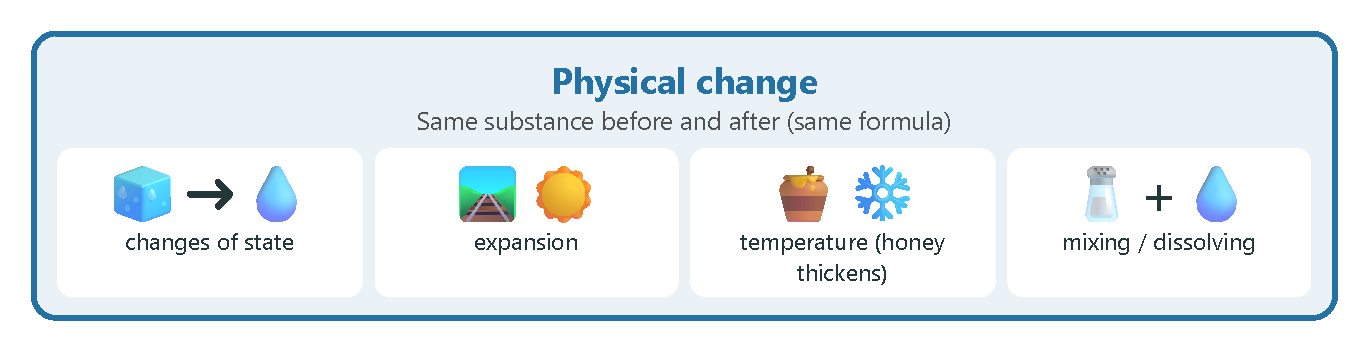
\includegraphics[width=0.85\textwidth]{FigurasSVG/Unit_5_Change_of_Matter/pdf/physical_change.pdf}
    \caption{Examples of physical changes: the substance is the same before and after.}
    \label{fig:u5_physical_change}
\end{figure}

\begin{itemize}
    \item \negsubro{Changes of temperature}: honey flows more easily when warm, but it is still honey.
    \item \negsubro{Changes of state}: ice, liquid water and water vapour are all \ch{H2O}.
    \item \negsubro{Expansion and contraction}: a metal expands when heated, but it is the same metal.
    \item \negsubro{Mixing}: iron and sulphur powder mixed together are still iron and sulphur; a magnet can separate them again.
\end{itemize}

\begin{exercise}
    Classify each physical change according to the four types above (change of temperature, change of state, expansion/contraction, mixing): a railway track on a hot day; freezing water to make ice cubes; mixing flour and sugar; honey thickening in winter.
    \begin{solu}
        Railway track: \textbf{expansion}. \\
        Ice cubes: \textbf{change of state}. \\
        Flour and sugar: \textbf{mixing}. \\
        Honey in winter: \textbf{change of temperature} (it becomes more viscous).
    \end{solu}
\end{exercise}

\begin{exercise}
    Explain why dissolving salt in water is a physical change, even though the salt seems to disappear.
    \begin{solu}
        No new substance is formed: the salt is still \ch{NaCl} and the water is still \ch{H2O}, only mixed. We can get the salt back unchanged just by evaporating the water.
    \end{solu}
\end{exercise}

\subsection{Chemical changes}

\begin{definition}[Chemical change]
    A change in which \textbf{new substances} appear, with a different formula and different properties.
\end{definition}

\begin{figure}[H]
    \centering
    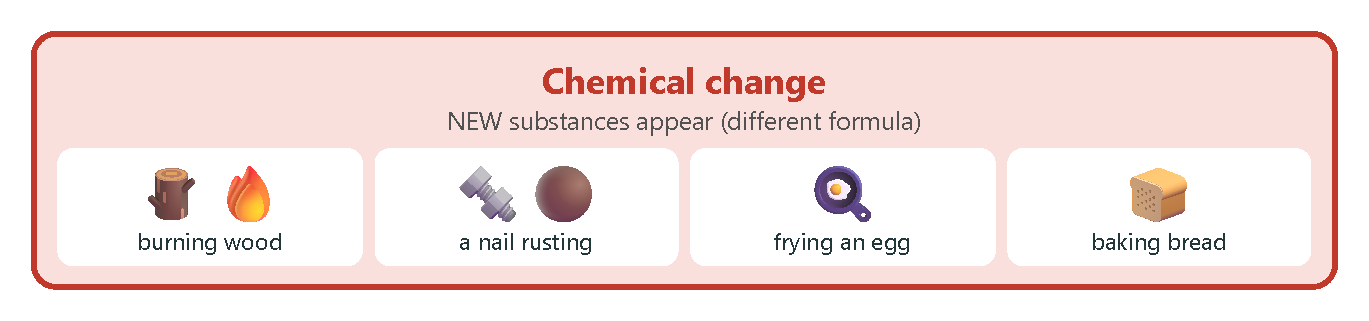
\includegraphics[width=0.85\textwidth]{FigurasSVG/Unit_5_Change_of_Matter/pdf/chemical_change.pdf}
    \caption{Examples of chemical changes: new substances appear.}
    \label{fig:u5_chemical_change}
\end{figure}

\begin{itemize}
    \item \negsubro{Combustion}: when wood, paper or the gas of a cooker burns, it reacts with the oxygen of the air and turns into new substances, such as carbon dioxide, water vapour and ash.
    \item \negsubro{Oxidation}: a nail left outdoors slowly reacts with oxygen and water and becomes covered in rust, a brown substance that is no longer iron.
    \item \negsubro{Cooking food}: when we fry an egg or bake bread, new substances with a different colour, taste and texture are formed; we cannot get the raw egg back.
    \item \negsubro{Decomposition}: a substance breaks down into simpler ones, for example when an electric current splits water into hydrogen and oxygen.
\end{itemize}

\begin{example}
    \begin{itemize}
        \item Passing an electric current through water (\ch{H2O}) produces two new substances: hydrogen (\ch{H2}) and oxygen (\ch{O2}).
        \item Heating a mixture of iron and sulphur produces iron sulphide (\ch{FeS}), a new substance that is \textbf{not} attracted by a magnet, unlike iron.
    \end{itemize}
\end{example}

\subsubsection*{Physical or chemical change?}

To decide whether a change is physical or chemical, we ask: \textbf{is there a new substance at the end?} Figure~\ref{fig:u5_changes_signs} compares both types of change and shows the \textbf{clues} that tell us a chemical change is happening.

\begin{figure}[H]
    \centering
    % [FIGURA ORIGINAL] \includegraphics[width=\textwidth]{Unit_5/changes_signs}
    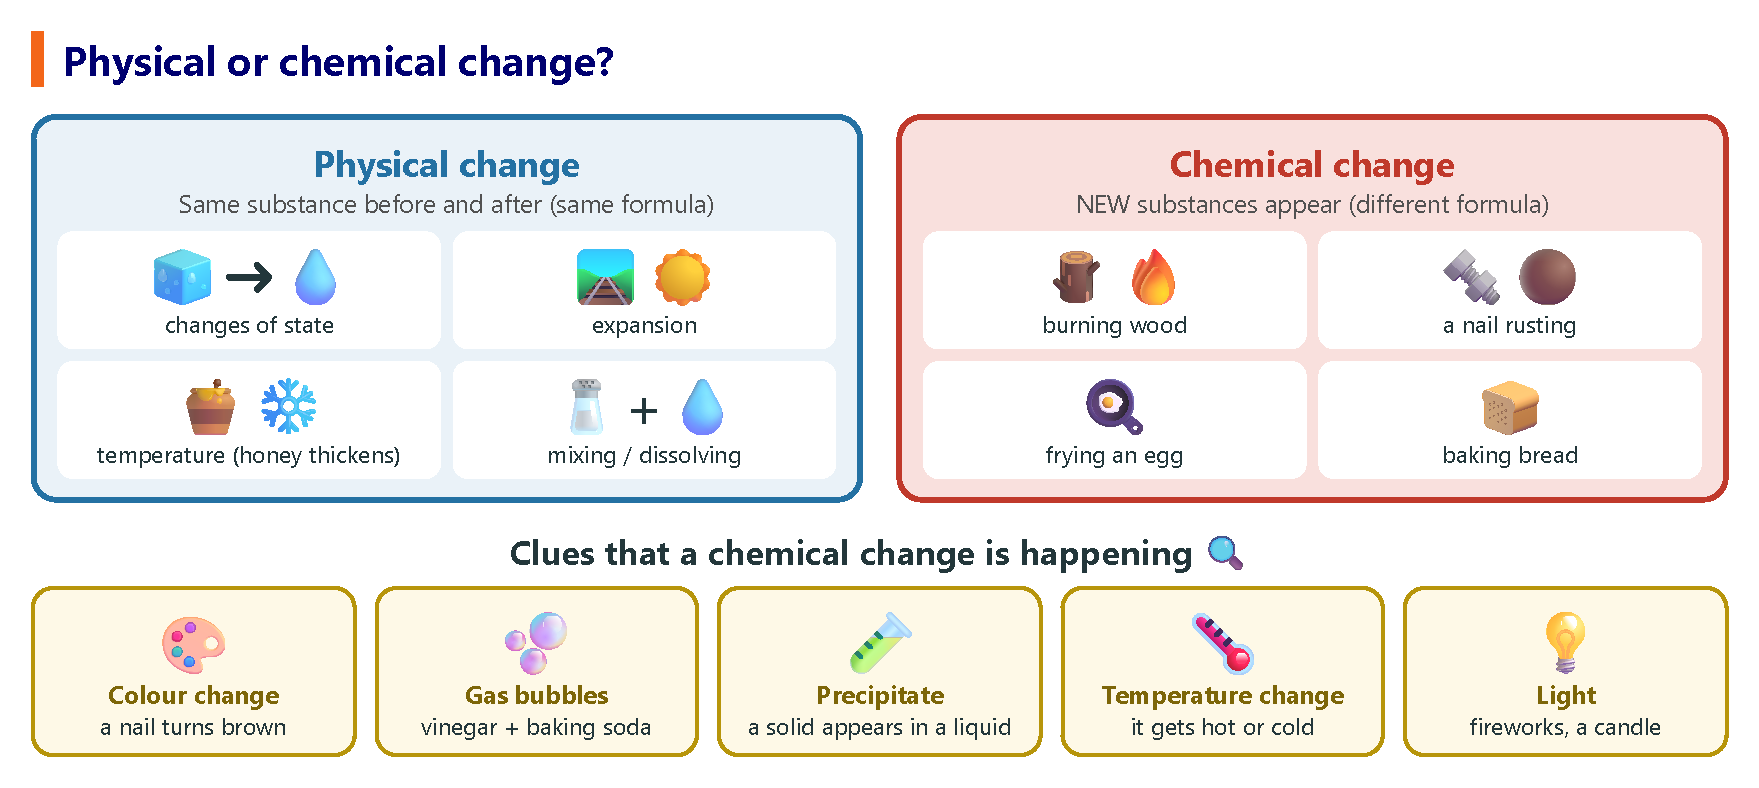
\includegraphics[width=\textwidth]{FigurasSVG/Unit_5_Change_of_Matter/pdf/changes_signs.pdf}
    \caption{Examples of physical and chemical changes, and the clues that tell us a chemical change is happening.}
    \label{fig:u5_changes_signs}
\end{figure}

\begin{impt}
    The clues in the figure suggest a chemical change, but the only \textbf{certain} proof is that new substances, with different properties, have appeared.
\end{impt}

\begin{exercise}
    Classify each transformation as a \textbf{physical} or a \textbf{chemical} change: chopping wood; lighting a candle; burning wood; beating an egg; a key rusting; alcohol evaporating; moulding clay; frying an egg; filtering water with sand; making mayonnaise; iodine subliming.
    \begin{solu}
        \textbf{Physical}: chopping wood, beating an egg, alcohol evaporating, moulding clay, filtering water, making mayonnaise, iodine subliming. \\
        \textbf{Chemical}: lighting a candle, burning wood, a key rusting, frying an egg.
    \end{solu}
\end{exercise}

\begin{exercise}
    Aluminium is obtained from bauxite by passing an electric current through the molten mineral, and later it can be melted down and reused many times. Are these two processes physical or chemical changes?
    \begin{solu}
        Obtaining aluminium from bauxite: \textbf{chemical} (aluminium oxide is transformed into metallic aluminium, a new substance). \\
        Melting aluminium to reuse it: \textbf{physical} (only a change of state); that is why aluminium can be recycled again and again.
    \end{solu}
\end{exercise}

\begin{exercise}
    Is each observation more likely a \textbf{physical} or a \textbf{chemical} change? Ice cubes crack in a warm drink; bubbles appear when vinegar is poured onto baking soda; a nail slowly turns orange-brown outdoors; sugar dissolves in tea; a firework explodes with bright colours.
    \begin{solu}
        Ice cracking: \textbf{physical}. \\
        Vinegar and baking soda: \textbf{chemical} (a gas, \ch{CO2}, is produced). \\
        Rusting nail: \textbf{chemical} (colour change, new substance). \\
        Sugar dissolving: \textbf{physical}. \\
        Firework: \textbf{chemical} (light, heat and new substances).
    \end{solu}
\end{exercise}

\begin{exercise}
    When a solution of silver nitrate is mixed with a solution of sodium chloride, a white solid appears and slowly settles at the bottom of the test tube. What type of change is it, and which clue tells you so?
    \begin{solu}
        A \textbf{chemical change}. The clue is the formation of a \textbf{precipitate} (an insoluble solid appearing inside a liquid).
    \end{solu}
\end{exercise}

%----------------------------------------------------------------------------------------

\section{Separation of the components of a mixture}

The substances in a mixture keep their own properties, so we can separate them using \textbf{physical methods}, which do not change them. We choose the method according to the \textbf{property} that makes the components different (size, density, magnetism, solubility, boiling point\ldots).

\subsection{Separation of heterogeneous mixtures}

\begin{figure}[H]
    \centering
    % [FIGURA ORIGINAL] \includegraphics[width=\textwidth]{Unit_5/separation_hetero}
    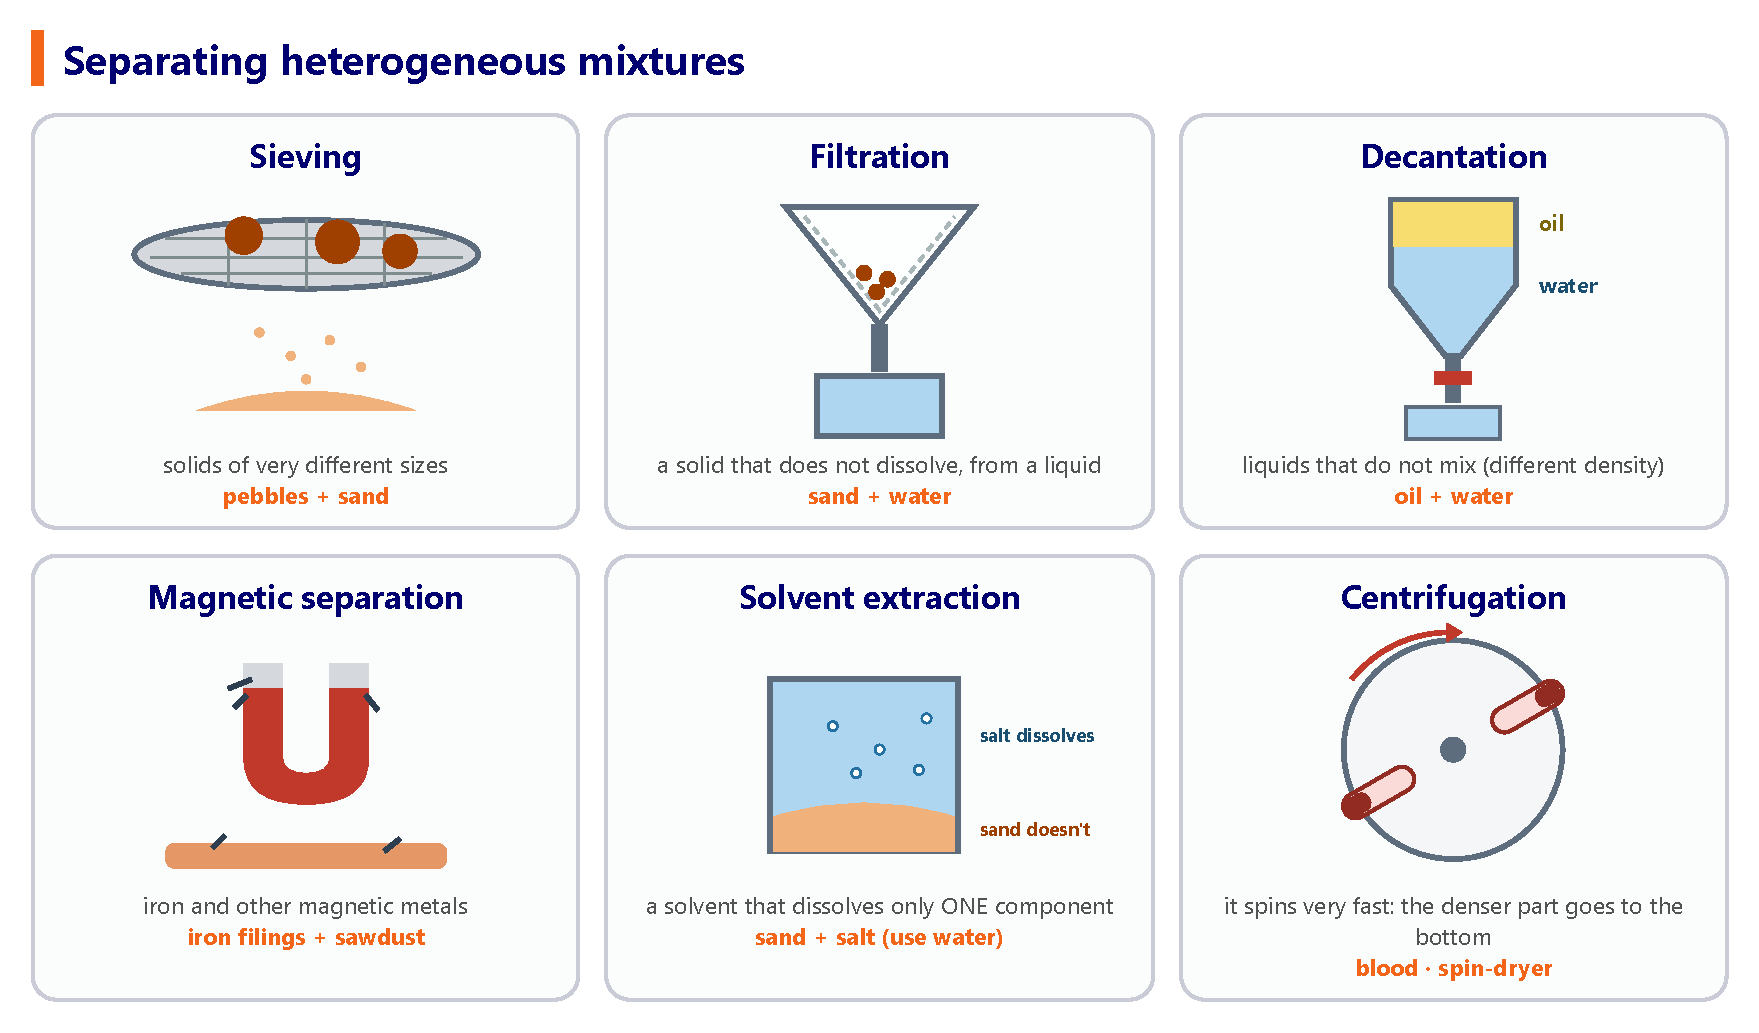
\includegraphics[width=\textwidth]{FigurasSVG/Unit_5_Change_of_Matter/pdf/separation_hetero.pdf}
    \caption{Methods to separate heterogeneous mixtures.}
    \label{fig:u5_separation_hetero}
\end{figure}

\begin{figure}[H]
    \centering
    % [FIGURA ORIGINAL] \includegraphics[width=0.95\textwidth]{Unit_5/filtration}
    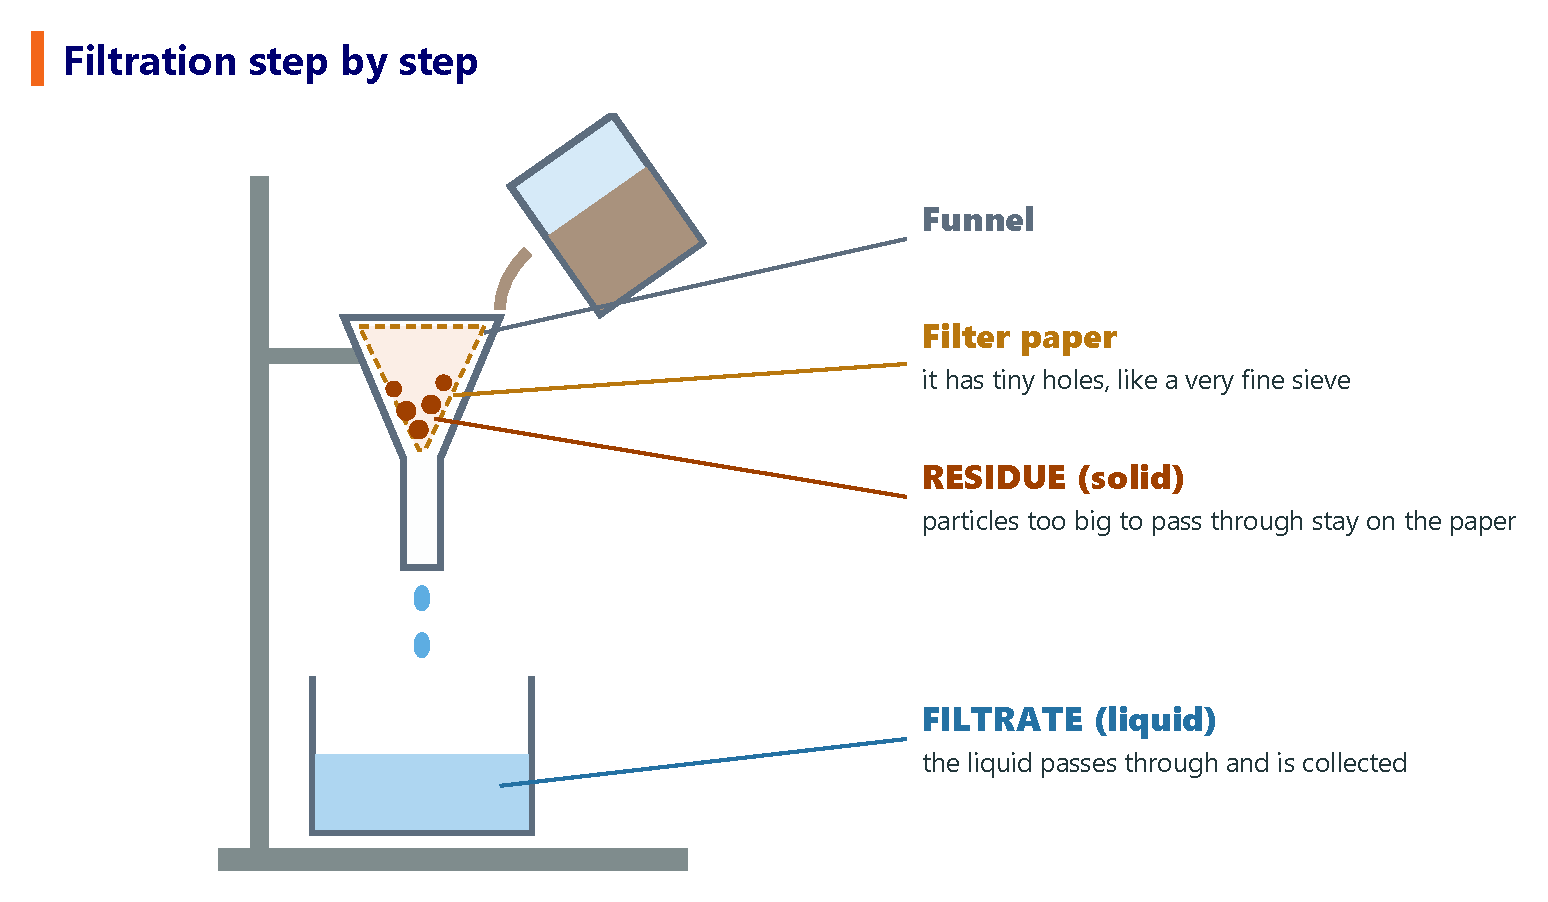
\includegraphics[width=0.95\textwidth]{FigurasSVG/Unit_5_Change_of_Matter/pdf/filtration.pdf}
    \caption{Filtration: the \textit{residue} stays on the paper and the \textit{filtrate} is collected below.}
    \label{fig:u5_filtration}
\end{figure}

Now let us see, \textbf{step by step}, how each of the other methods is carried out in the laboratory.

\begin{figure}[H]
    \centering
    % [FIGURA ORIGINAL] \includegraphics[width=\textwidth]{Unit_5/sieving_steps}
    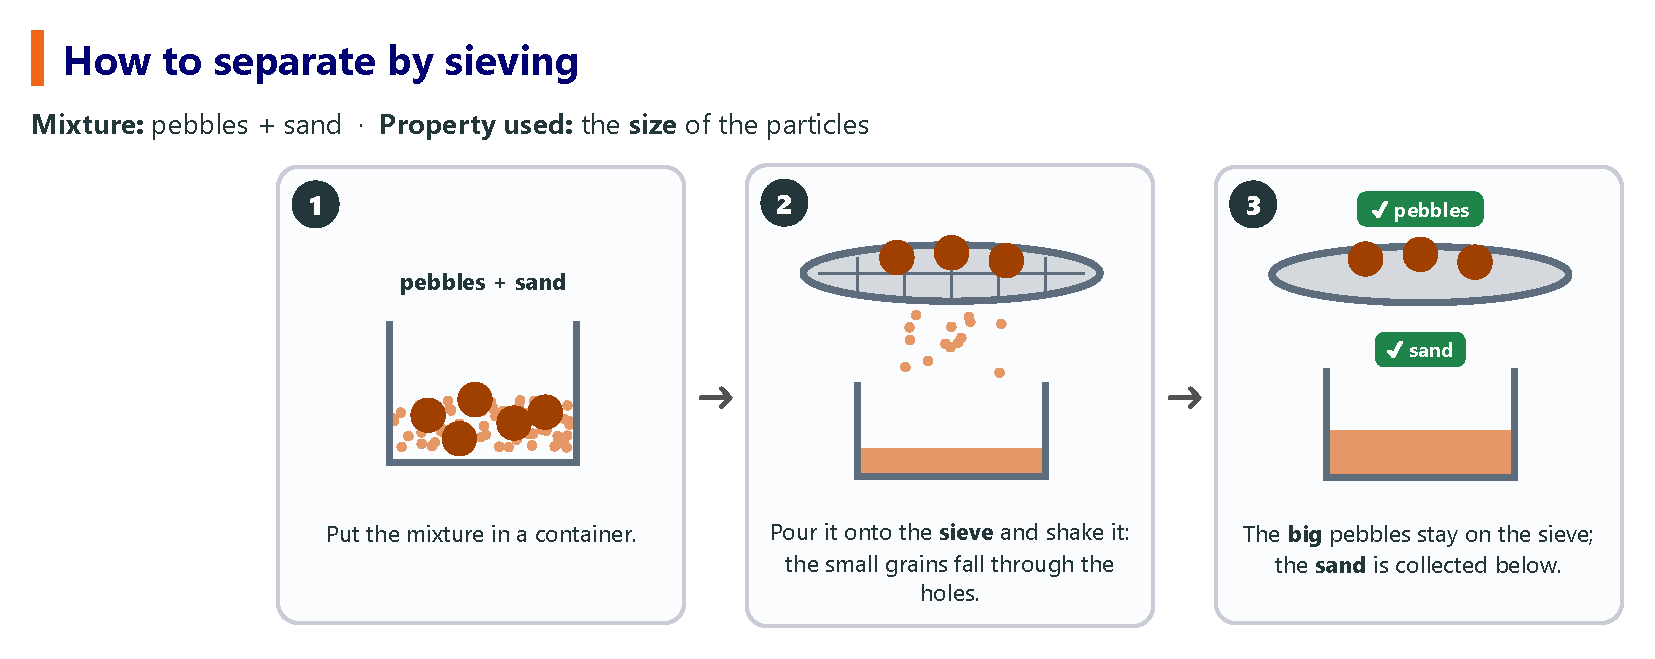
\includegraphics[width=\textwidth]{FigurasSVG/Unit_5_Change_of_Matter/pdf/sieving_steps.pdf}
    \caption{Sieving step by step.}
    \label{fig:u5_sieving_steps}
\end{figure}

\begin{figure}[H]
    \centering
    % [FIGURA ORIGINAL] \includegraphics[width=\textwidth]{Unit_5/decantation_steps}
    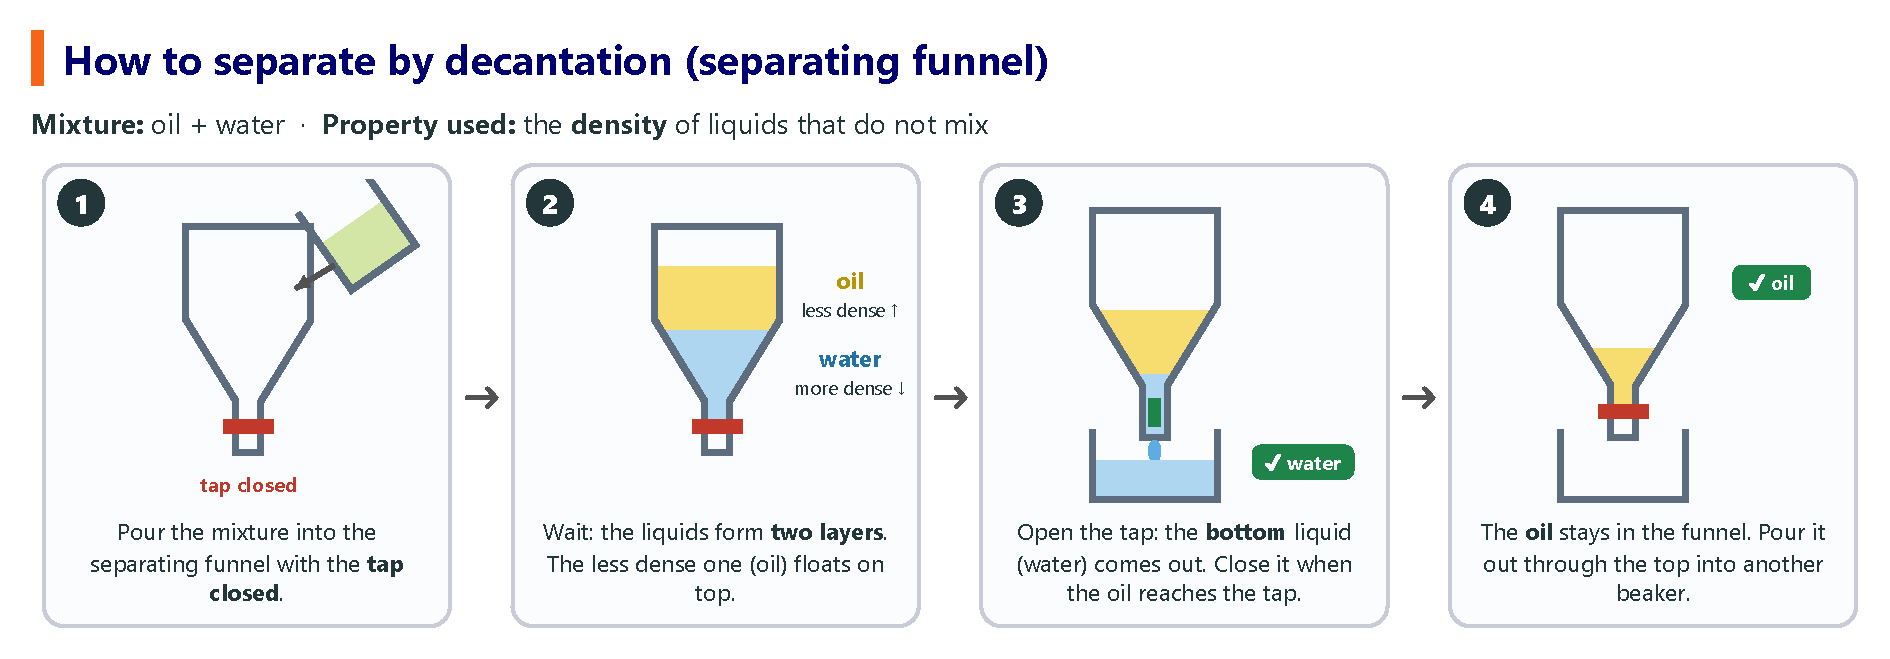
\includegraphics[width=\textwidth]{FigurasSVG/Unit_5_Change_of_Matter/pdf/decantation_steps.pdf}
    \caption{Decantation with a separating funnel, step by step.}
    \label{fig:u5_decantation_steps}
\end{figure}

\begin{figure}[H]
    \centering
    % [FIGURA ORIGINAL] \includegraphics[width=\textwidth]{Unit_5/magnetic_steps}
    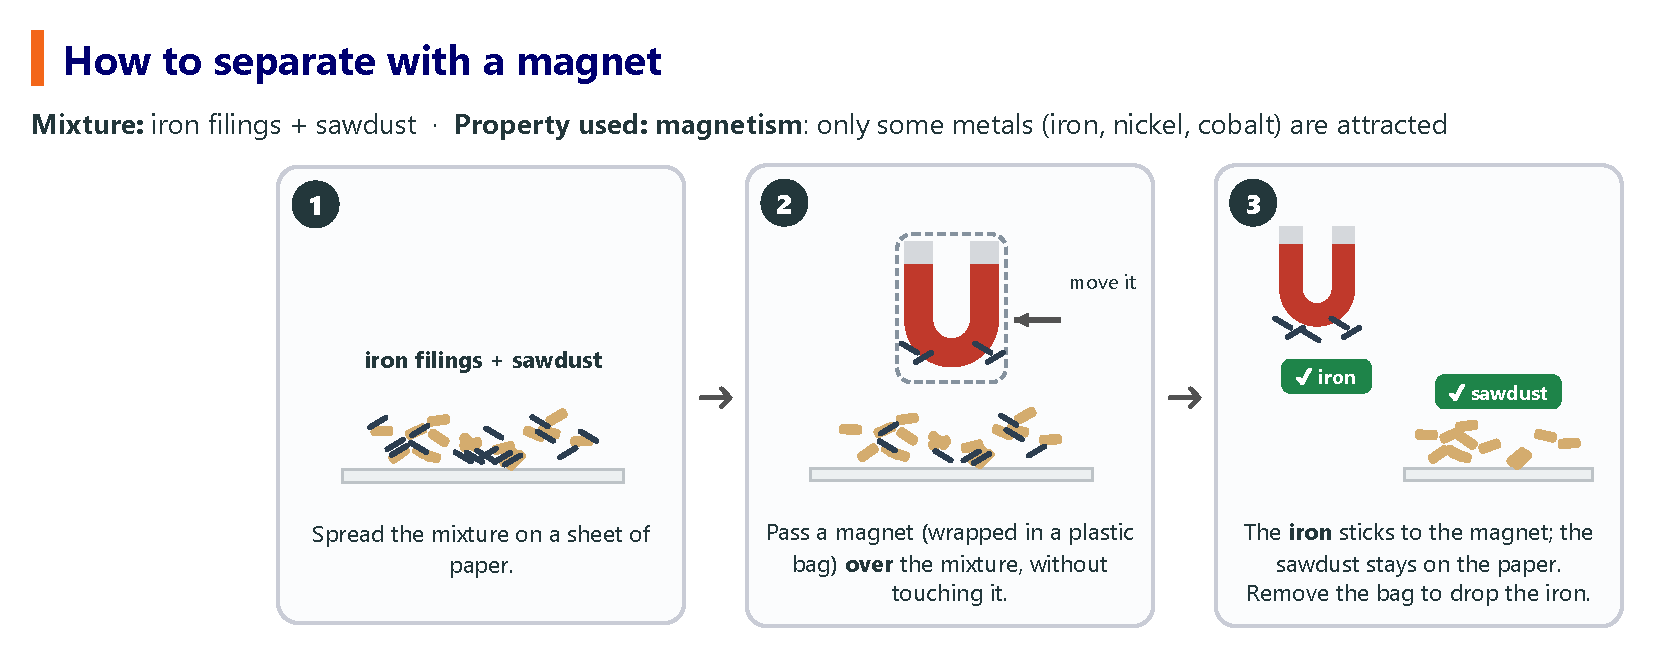
\includegraphics[width=\textwidth]{FigurasSVG/Unit_5_Change_of_Matter/pdf/magnetic_steps.pdf}
    \caption{Magnetic separation step by step.}
    \label{fig:u5_magnetic_steps}
\end{figure}

\begin{figure}[H]
    \centering
    % [FIGURA ORIGINAL] \includegraphics[width=\textwidth]{Unit_5/extraction_steps}
    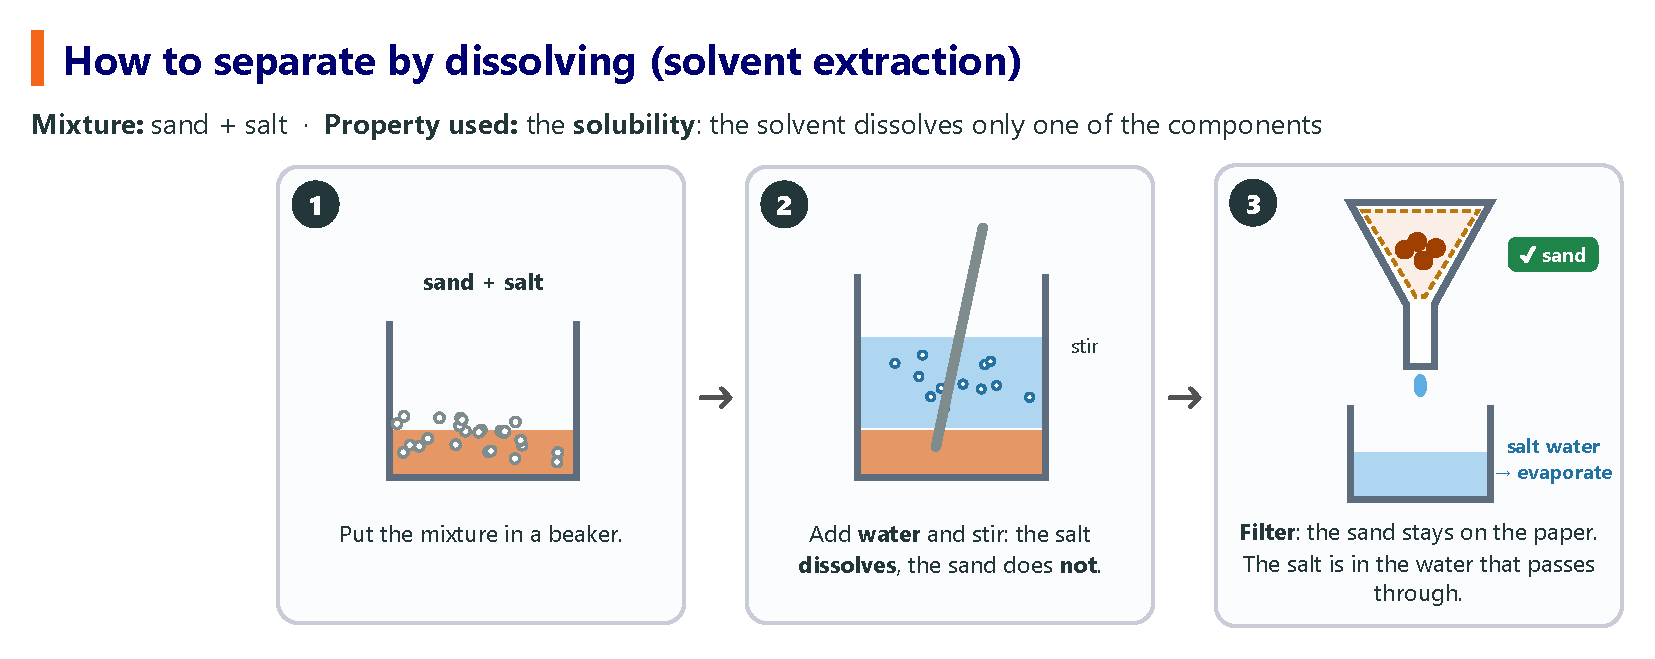
\includegraphics[width=\textwidth]{FigurasSVG/Unit_5_Change_of_Matter/pdf/extraction_steps.pdf}
    \caption{Solvent extraction (separating by dissolving) step by step.}
    \label{fig:u5_extraction_steps}
\end{figure}

\begin{figure}[H]
    \centering
    % [FIGURA ORIGINAL] \includegraphics[width=\textwidth]{Unit_5/centrifugation_steps}
    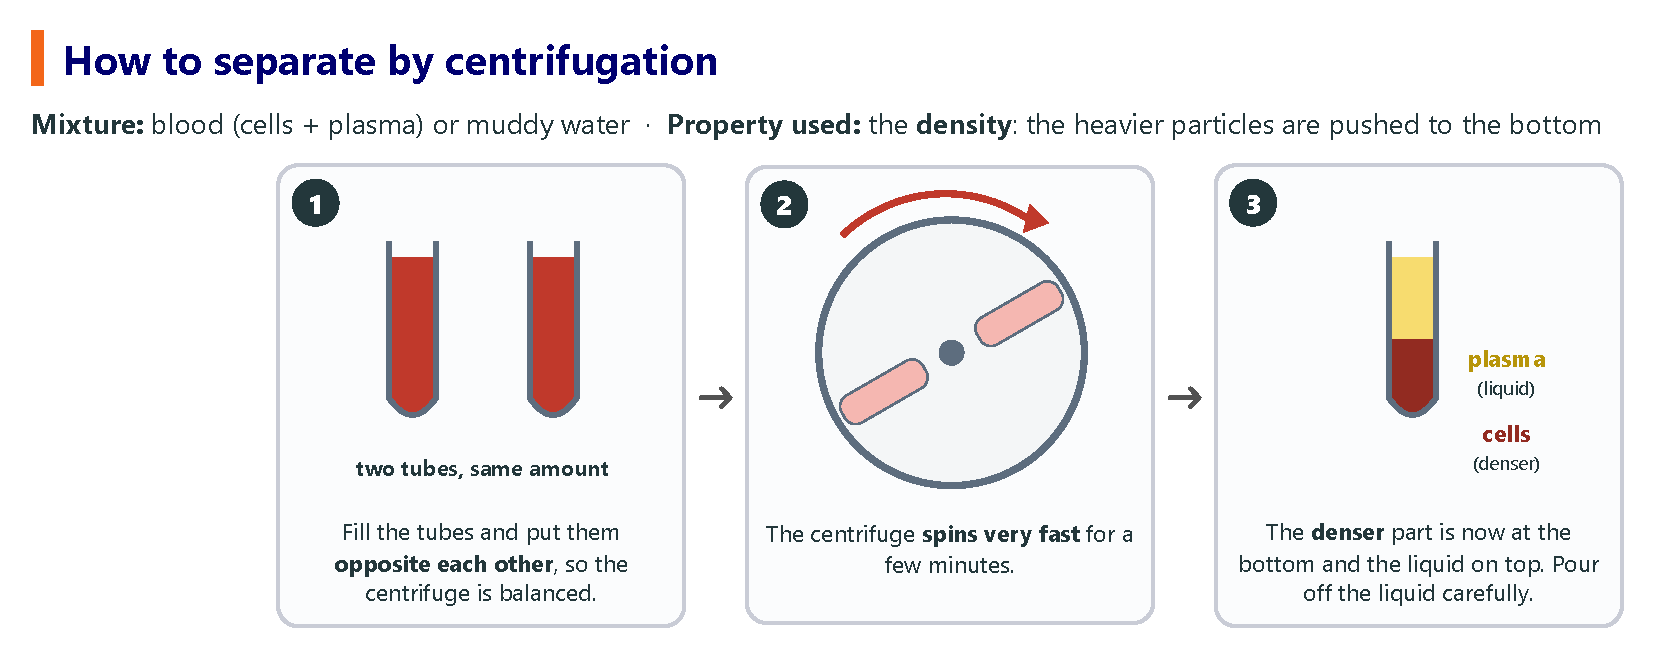
\includegraphics[width=\textwidth]{FigurasSVG/Unit_5_Change_of_Matter/pdf/centrifugation_steps.pdf}
    \caption{Centrifugation step by step.}
    \label{fig:u5_centrifugation_steps}
\end{figure}

\begin{exercise}
    Name the best separation method for each mixture, and justify your choice: gravel and fine sand; iron filings and wood shavings; a salad dressing made of vinegar and olive oil.
    \begin{solu}
        Gravel and sand: \textbf{sieving} (very different sizes). \\
        Iron filings and wood shavings: \textbf{magnetic separation} (only iron is attracted by a magnet). \\
        Vinegar and oil: \textbf{decantation} (liquids that do not mix, with different densities).
    \end{solu}
\end{exercise}

\begin{exercise}
    In a school laboratory, a small sample of muddy water is cleaned with a funnel and filter paper. In a water treatment plant, huge volumes of muddy water are left to stand in large tanks for several hours. Name the technique used in each case, and explain why the plant does not use filter paper.
    \begin{solu}
        Laboratory: \textbf{filtration}. Treatment plant: \textbf{decantation} (sedimentation). Filtering such huge volumes through paper would be far too slow and the filters would block; letting the soil settle under gravity is cheaper and works well for large quantities.
    \end{solu}
\end{exercise}

\subsection{Separation of homogeneous mixtures}

\begin{figure}[H]
    \centering
    % [FIGURA ORIGINAL] \includegraphics[width=\textwidth]{Unit_5/separation_homo}
    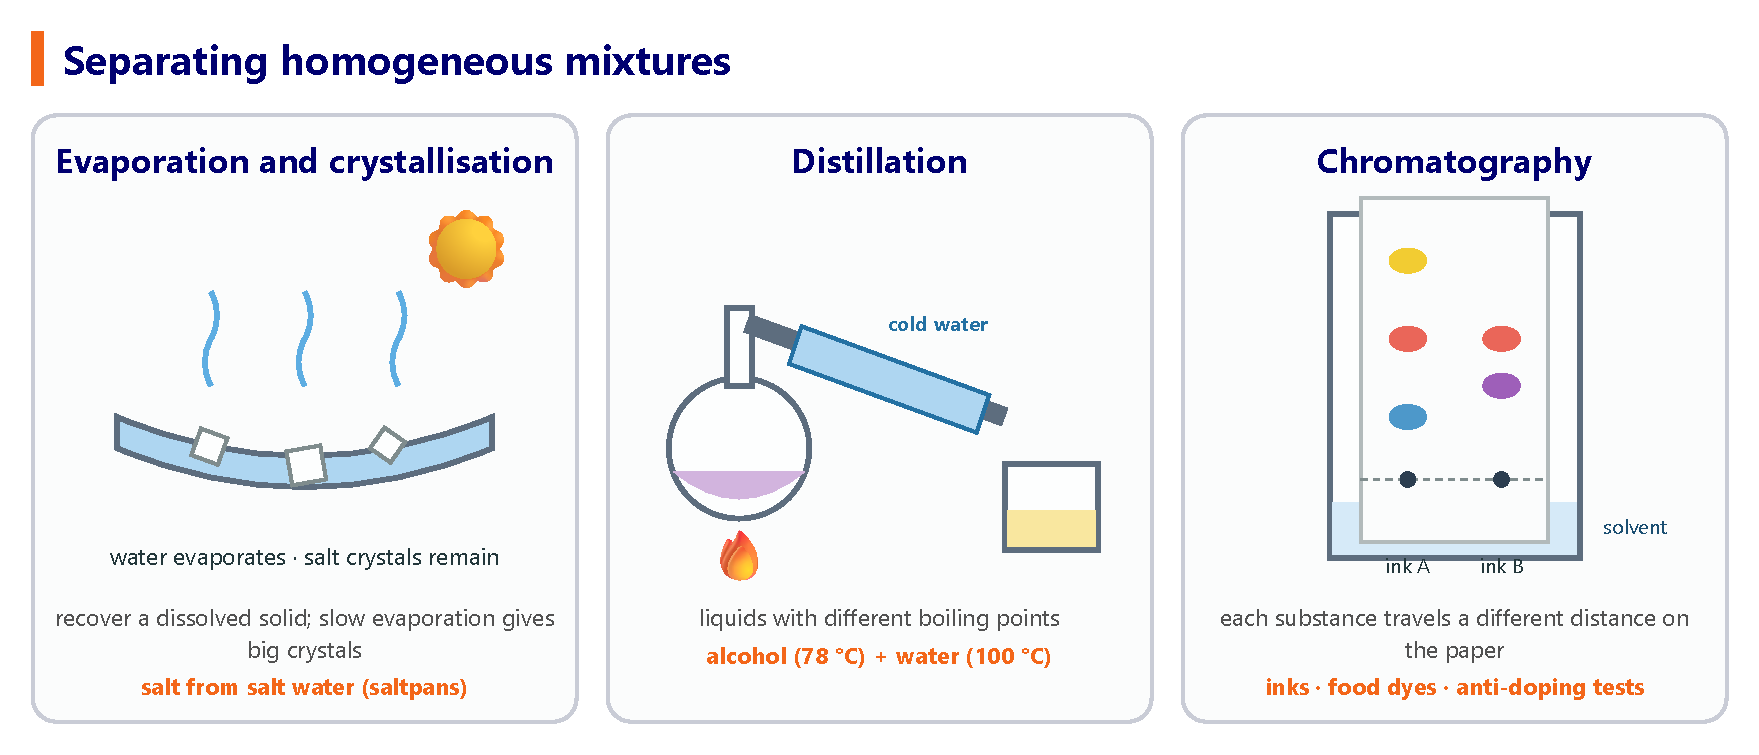
\includegraphics[width=\textwidth]{FigurasSVG/Unit_5_Change_of_Matter/pdf/separation_homo.pdf}
    \caption{Methods to separate homogeneous mixtures.}
    \label{fig:u5_separation_homo}
\end{figure}

\begin{figure}[H]
    \centering
    % [FIGURA ORIGINAL] \includegraphics[width=\textwidth]{Unit_5/distillation}
    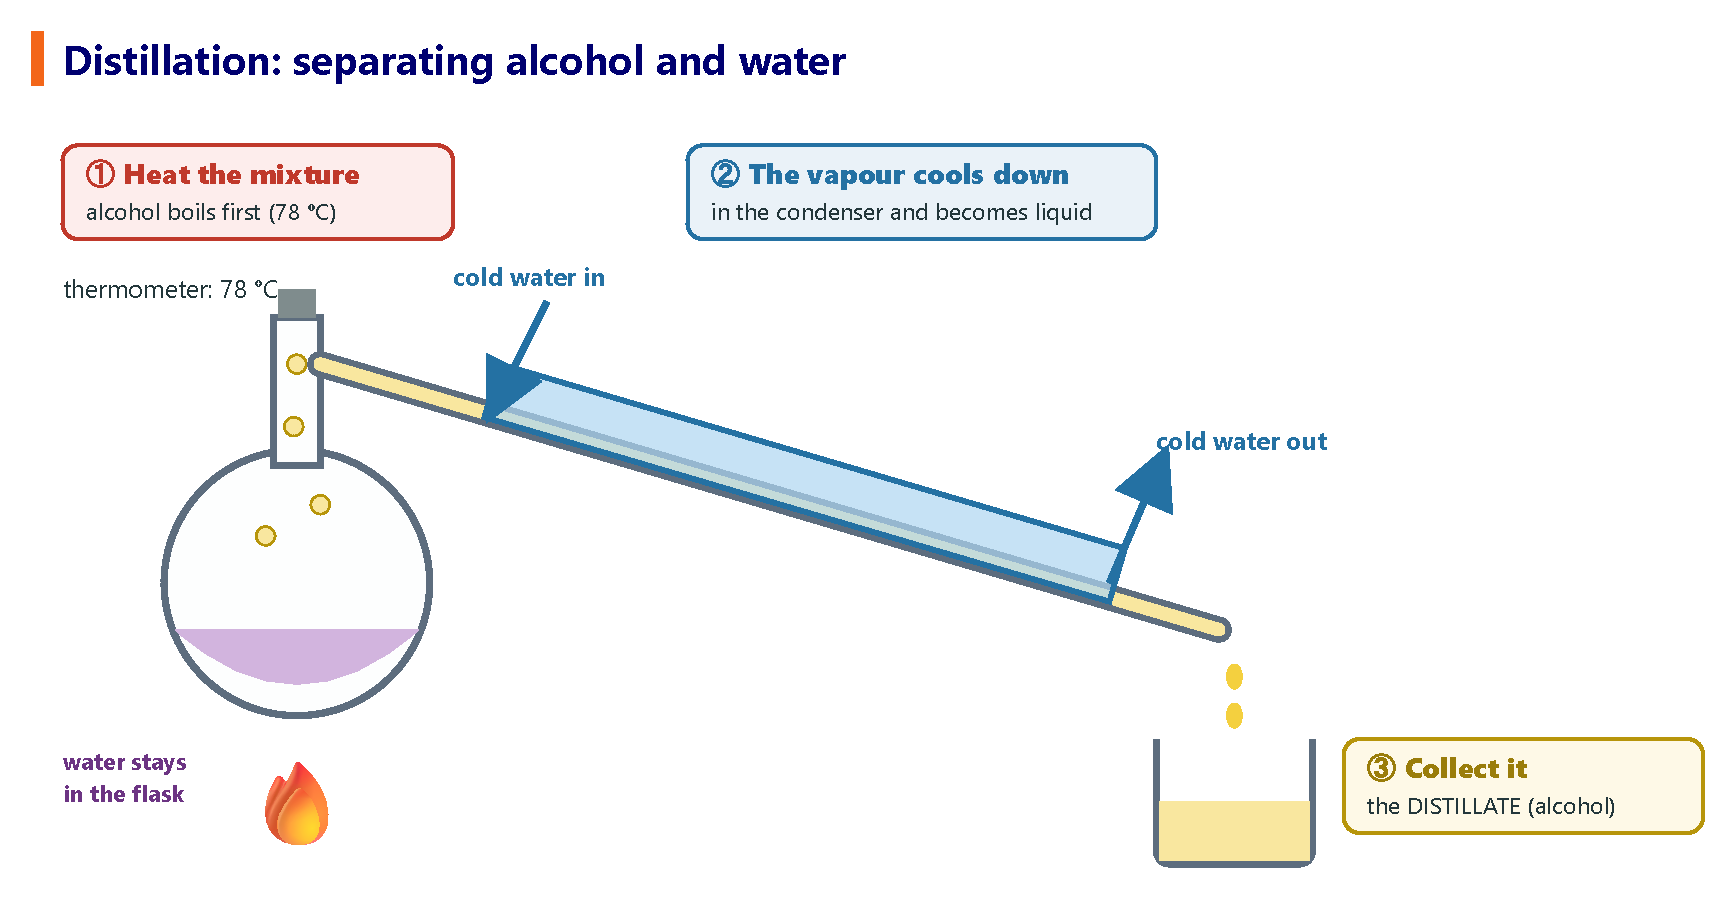
\includegraphics[width=\textwidth]{FigurasSVG/Unit_5_Change_of_Matter/pdf/distillation.pdf}
    \caption{Distillation: the liquid with the lower boiling point evaporates first and is condensed in the condenser.}
    \label{fig:u5_distillation}
\end{figure}

\begin{figure}[H]
    \centering
    % [FIGURA ORIGINAL] \includegraphics[width=\textwidth]{Unit_5/evaporation_steps}
    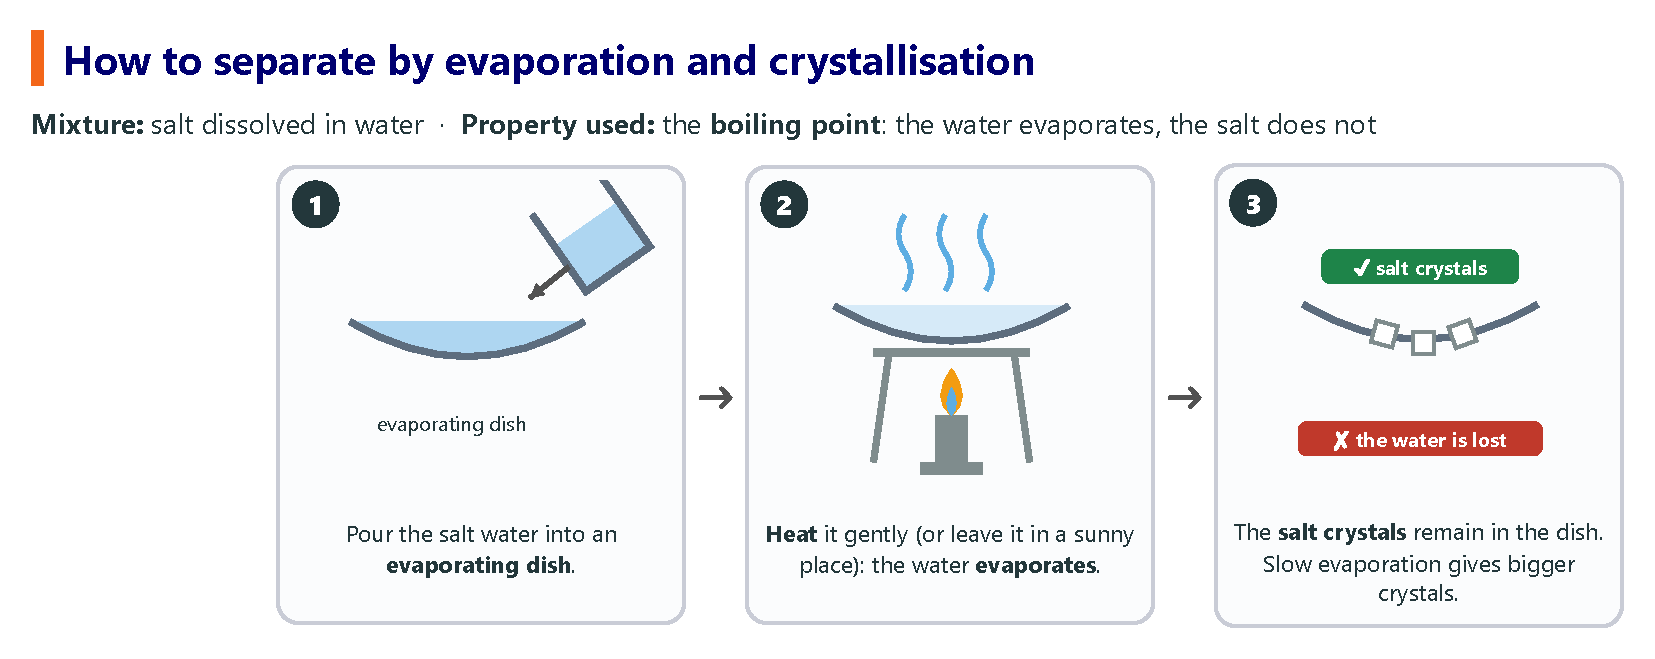
\includegraphics[width=\textwidth]{FigurasSVG/Unit_5_Change_of_Matter/pdf/evaporation_steps.pdf}
    \caption{Evaporation and crystallisation step by step.}
    \label{fig:u5_evaporation_steps}
\end{figure}

\begin{figure}[H]
    \centering
    % [FIGURA ORIGINAL] \includegraphics[width=\textwidth]{Unit_5/chromatography_steps}
    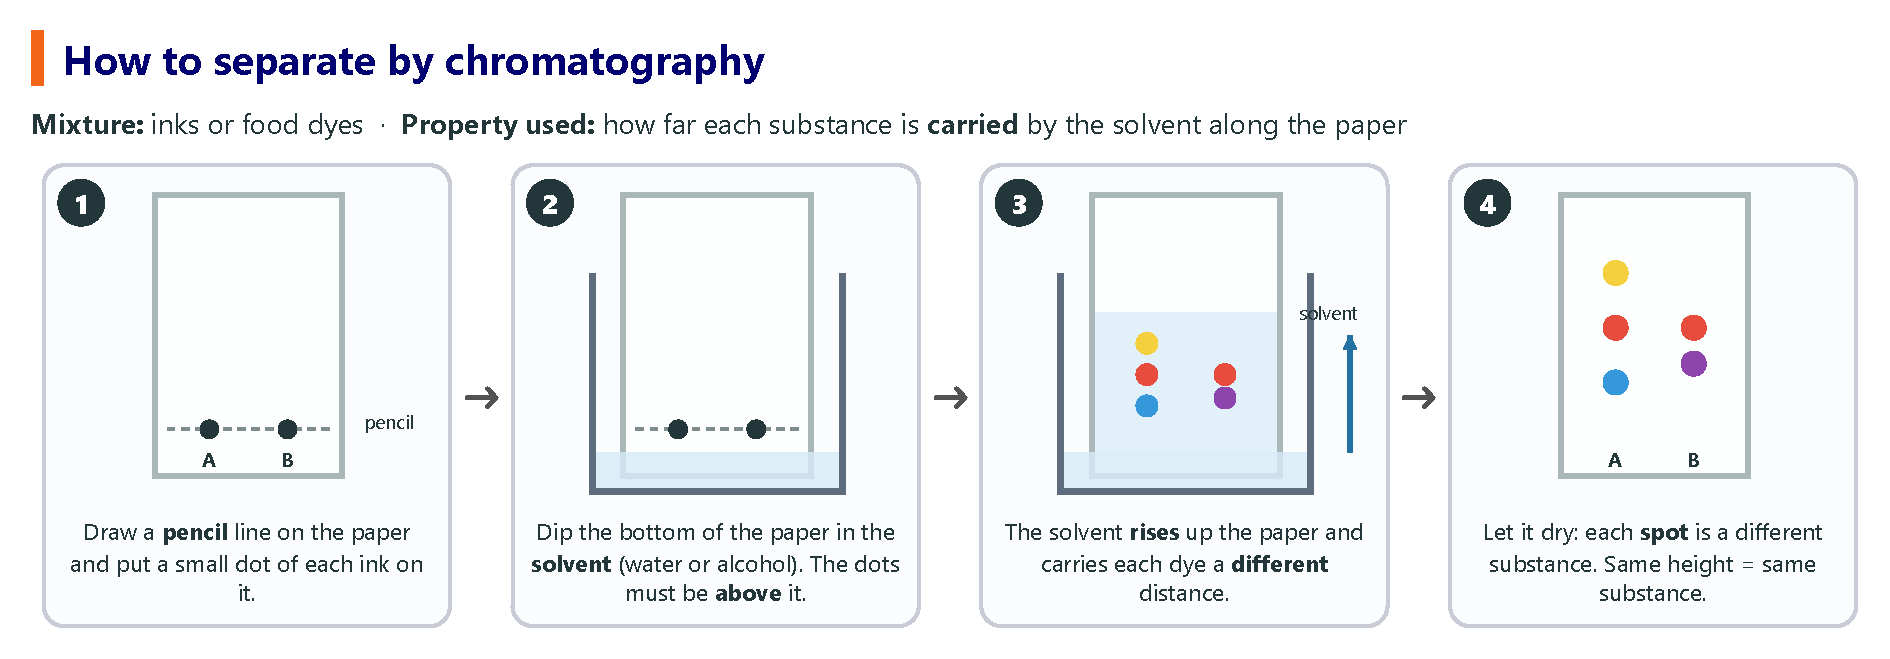
\includegraphics[width=\textwidth]{FigurasSVG/Unit_5_Change_of_Matter/pdf/chromatography_steps.pdf}
    \caption{Paper chromatography step by step.}
    \label{fig:u5_chromatography_steps}
\end{figure}

\begin{didyouknow}
    Many countries with little rain, such as the Canary Islands, get their drinking water from the sea in \textbf{desalination plants}. The seawater is filtered first, and then the salts are removed by distillation or by pushing the water through special membranes.
\end{didyouknow}

\begin{exercise}
    A perfume is a homogeneous mixture of several fragrant substances dissolved in alcohol, each with a different boiling point. Which technique would you use to recover the alcohol, and which property does it use?
    \begin{solu}
        \textbf{Distillation}. It uses the \textbf{different boiling points}: the substance with the lowest boiling point evaporates first and can be condensed and collected separately.
    \end{solu}
\end{exercise}

\begin{exercise}
    A forensic scientist needs to know whether the ink on a note matches the ink from a suspect's pen. Which technique should be used, and how does it allow the two inks to be compared?
    \begin{solu}
        \textbf{Chromatography}. A drop of each ink is placed on filter paper with a solvent; each dye travels a different distance, giving a pattern of coloured spots. If both patterns are the same, the inks are very likely the same.
    \end{solu}
\end{exercise}

\begin{exercise}
    Put these steps of the distillation of a mixture of alcohol and water in the correct order: the alcohol condenses; the mixture reaches the boiling point of alcohol; the alcohol vaporises; the liquid alcohol is collected in another container.
    \begin{solu}
        1.\ The mixture reaches the boiling point of alcohol (\qty{78}{\celsius}). \\
        2.\ The alcohol vaporises. \\
        3.\ The alcohol condenses in the condenser. \\
        4.\ The liquid alcohol is collected in another container.
    \end{solu}
\end{exercise}

\subsection{Applying separation techniques together}

Real mixtures often need \textbf{several} methods, one after another:

\begin{figure}[H]
    \centering
    % [FIGURA ORIGINAL] \includegraphics[width=\textwidth]{Unit_5/separation_steps}
    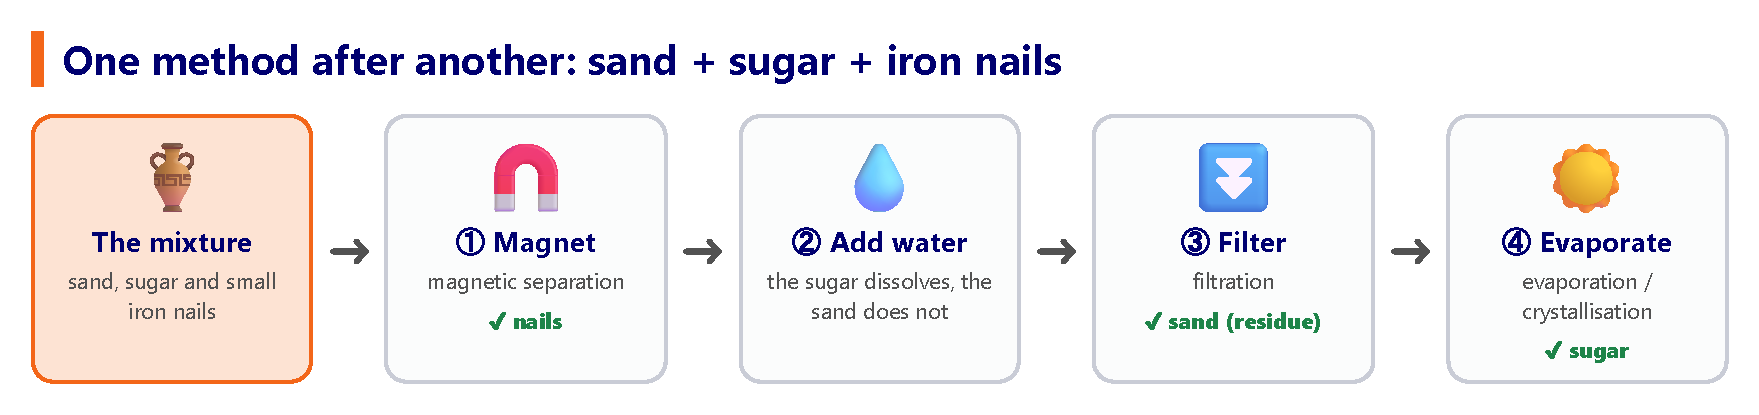
\includegraphics[width=\textwidth]{FigurasSVG/Unit_5_Change_of_Matter/pdf/separation_steps.pdf}
    \caption{Separating a mixture of three components step by step.}
    \label{fig:u5_separation_steps}
\end{figure}

\begin{impt}
    \negsubro{What do I keep and what do I throw away?} After each step the mixture is divided into two parts. Before starting, read the exercise carefully to know \textbf{what you want to obtain}, and after each step decide what to do with each part:
    \begin{itemize}
        \item \textcolor{green!50!black}{\textbf{KEEP}}: it is one of the substances that we want to obtain.
        \item \textcolor{blue!70!black}{\textbf{NEXT STEP}}: it is still a mixture, so we keep separating it.
        \item \textcolor{red!70!black}{\textbf{DISCARD}}: we do not need it (we throw it away or take it to a recycling point).
    \end{itemize}
    Be especially careful when there is a \textbf{solid and a liquid}, as in filtration: the solid that stays on the paper is the \textbf{residue}, and the liquid that passes through is the \textbf{filtrate}. Either of them can be the part we keep, the part that goes on to the next step or the part we throw away: it depends on what we want to obtain.
\end{impt}

\begin{example}
    \textbf{Worked example 1. We have a mixture of sand, salt and iron filings. We want to obtain the three components separately.}
\end{example}

\begin{figure}[H]
    \centering
    % [FIGURA ORIGINAL] \includegraphics[width=\textwidth]{Unit_5/example_sand_salt_iron}
    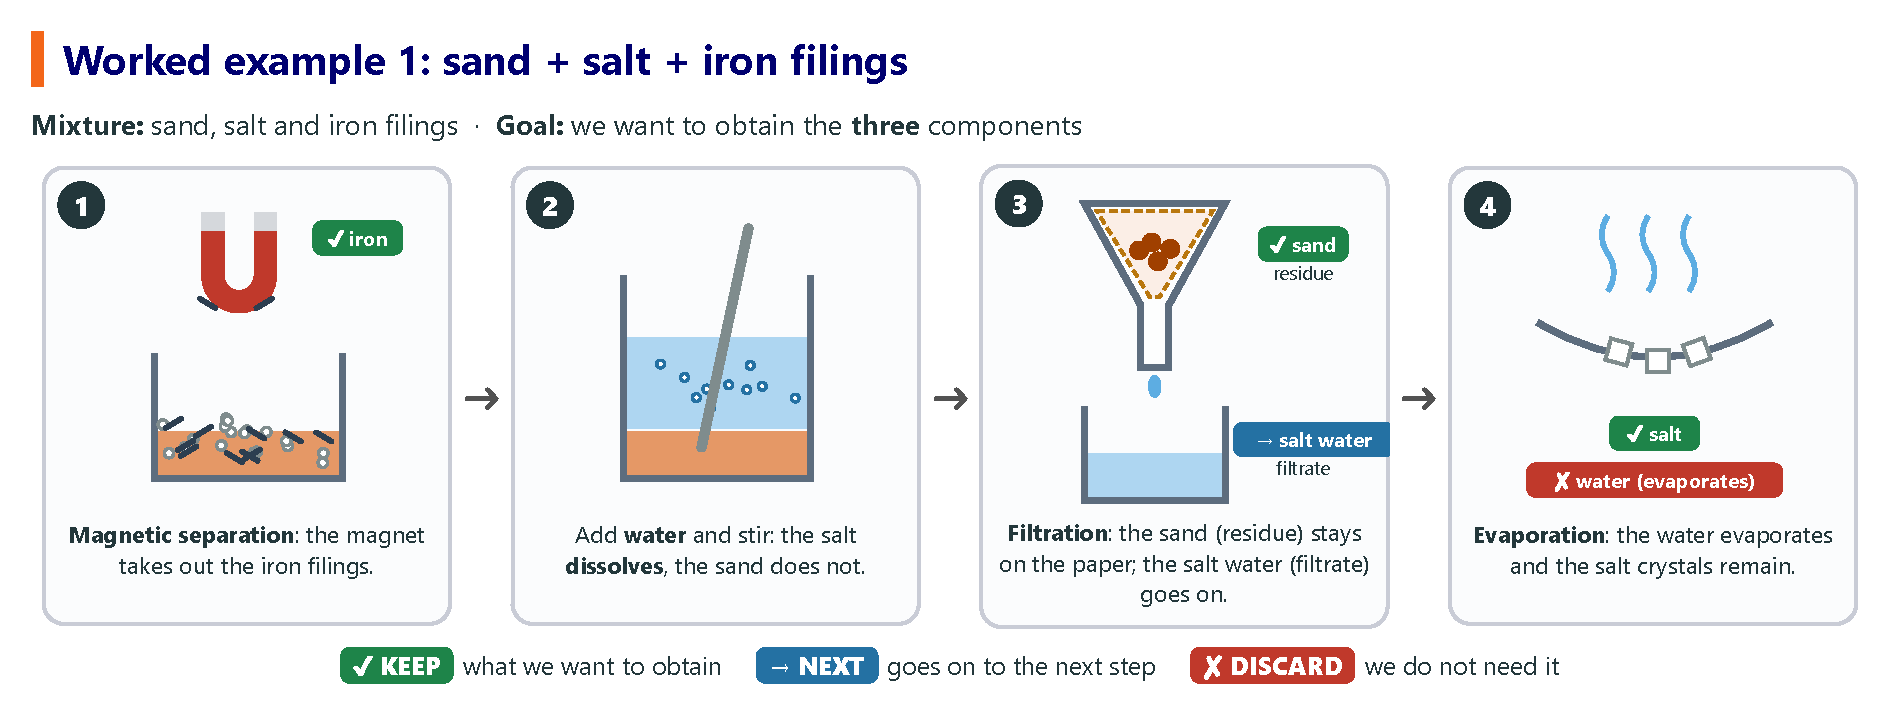
\includegraphics[width=\textwidth]{FigurasSVG/Unit_5_Change_of_Matter/pdf/example_sand_salt_iron.pdf}
    \caption{Worked example 1: separating sand, salt and iron filings.}
    \label{fig:u5_example_sand_salt_iron}
\end{figure}

\begin{enumerate}[label=\numberballmDarkTeal]
    \item \textbf{Magnetic separation.} We pass a magnet over the mixture. Only the iron is attracted. \textcolor{green!50!black}{\textbf{Keep}}: iron filings. \textcolor{blue!70!black}{\textbf{Next step}}: sand + salt.
    \item \textbf{Dissolving.} We add water to the sand and salt and stir. The salt dissolves; the sand does not.
    \item \textbf{Filtration.} We filter the mixture. \textcolor{green!50!black}{\textbf{Keep}}: the sand (\textbf{residue}), which we leave to dry. \textcolor{blue!70!black}{\textbf{Next step}}: the salt water (\textbf{filtrate}).
    \item \textbf{Evaporation.} We heat the salt water in an evaporating dish. \textcolor{green!50!black}{\textbf{Keep}}: the salt crystals. The water evaporates: we \textcolor{red!70!black}{\textbf{lose}} it, but we did not need it.
\end{enumerate}

\begin{tcolorbox}[enhanced, breakable, colback=yellow!6!white, colframe=ocre, boxrule=0.8pt, arc=2mm,
    fonttitle=\sffamily\bfseries, title={How to write it in your notebook}]
    \textbf{Mixture}: sand + salt + iron filings. \quad \textbf{Goal}: obtain the three components.

    \begin{tabular}{@{}p{0.3cm}>{\raggedright\arraybackslash}p{2.9cm}>{\raggedright\arraybackslash}p{3.9cm}>{\raggedright\arraybackslash}p{4.2cm}@{}}
        \toprule
        & \textbf{Method} & \textbf{Why? (property)} & \textbf{Result} \\
        \midrule
        1 & Magnetic separation & iron is attracted by magnets & \textbf{iron} (keep); sand + salt (next) \\
        2 & Dissolve in water & salt is soluble, sand is not & sand + salt water (next) \\
        3 & Filtration & sand does not pass through the paper & residue: \textbf{sand} (keep); filtrate: salt water (next) \\
        4 & Evaporation & water evaporates, salt does not & \textbf{salt} (keep); water (lost) \\
        \bottomrule
    \end{tabular}
\end{tcolorbox}

\begin{example}
    \textbf{Worked example 2. A bucket contains muddy, oily water: sand, oil and water. We want to obtain clean water.}
\end{example}

\begin{figure}[H]
    \centering
    % [FIGURA ORIGINAL] \includegraphics[width=\textwidth]{Unit_5/example_sand_oil_water}
    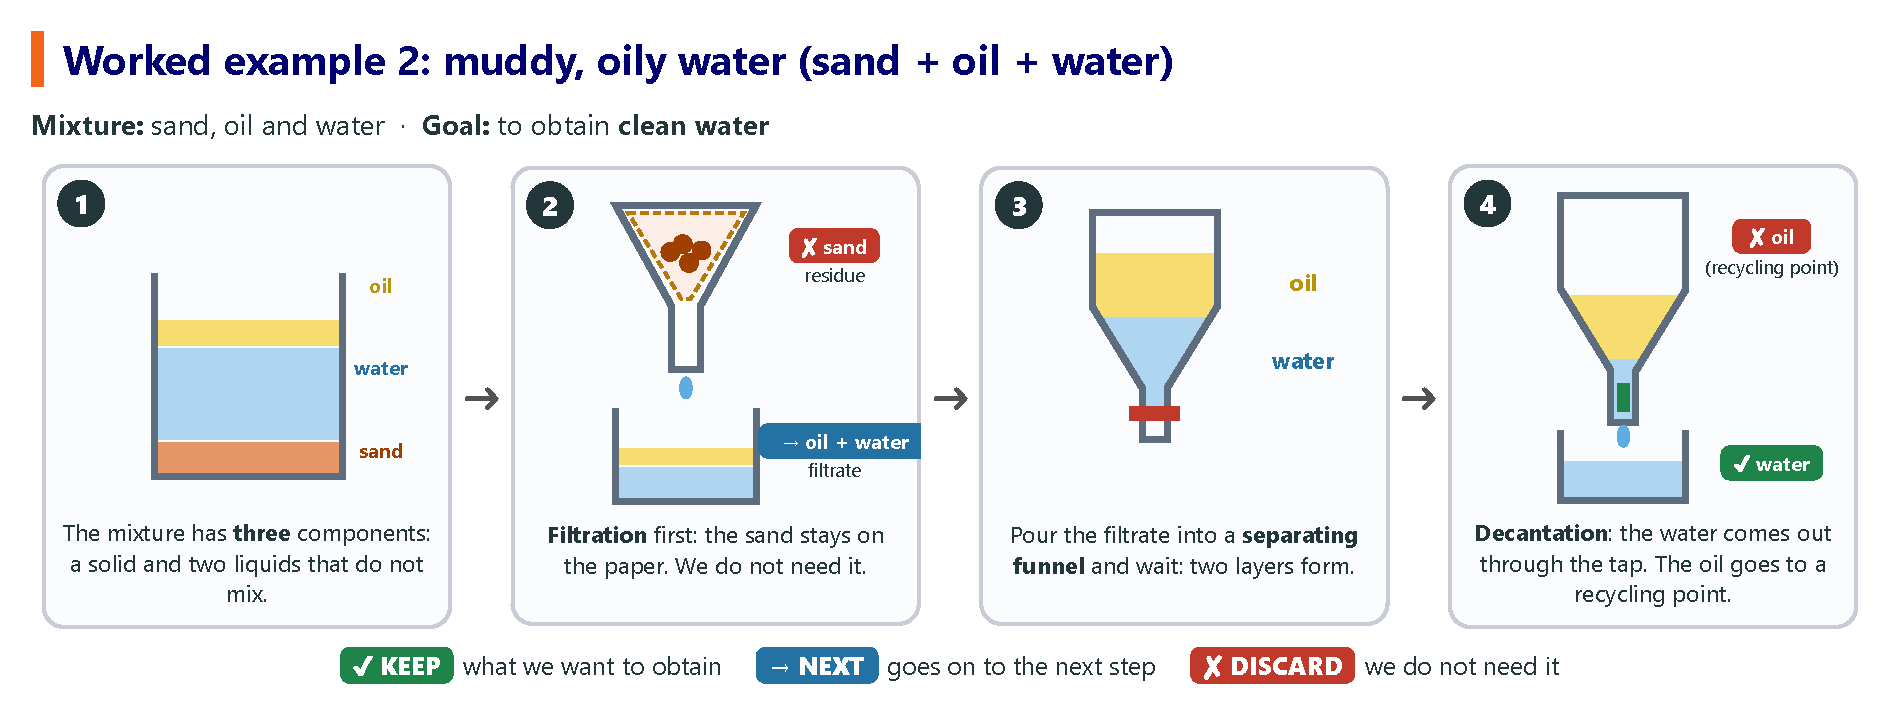
\includegraphics[width=\textwidth]{FigurasSVG/Unit_5_Change_of_Matter/pdf/example_sand_oil_water.pdf}
    \caption{Worked example 2: obtaining clean water from a mixture of sand, oil and water.}
    \label{fig:u5_example_sand_oil_water}
\end{figure}

\begin{enumerate}[label=\numberballmDarkTeal]
    \item We look at the mixture: one solid (sand) and two liquids that do not mix (oil and water).
    \item \textbf{Filtration first}, so that the sand does not block the tap of the separating funnel. \textcolor{red!70!black}{\textbf{Discard}}: the sand (\textbf{residue}), because we only want the water. \textcolor{blue!70!black}{\textbf{Next step}}: oil + water (\textbf{filtrate}).
    \item We pour the filtrate into a \textbf{separating funnel} and wait until two layers form: the oil, less dense, on top; the water, more dense, at the bottom.
    \item \textbf{Decantation.} We open the tap and let the water out, closing it when the oil reaches the tap. \textcolor{green!50!black}{\textbf{Keep}}: the clean water. \textcolor{red!70!black}{\textbf{Discard}}: the oil, which must \textbf{never} be poured down the sink: we take it to a recycling point.
\end{enumerate}

\begin{tcolorbox}[enhanced, breakable, colback=yellow!6!white, colframe=ocre, boxrule=0.8pt, arc=2mm,
    fonttitle=\sffamily\bfseries, title={How to write it in your notebook}]
    \textbf{Mixture}: sand + oil + water. \quad \textbf{Goal}: obtain clean water.

    \begin{tabular}{@{}p{0.3cm}>{\raggedright\arraybackslash}p{2.9cm}>{\raggedright\arraybackslash}p{3.9cm}>{\raggedright\arraybackslash}p{4.2cm}@{}}
        \toprule
        & \textbf{Method} & \textbf{Why? (property)} & \textbf{Result} \\
        \midrule
        1 & Filtration & sand does not pass through the paper & residue: sand (discard); filtrate: oil + water (next) \\
        2 & Decantation (separating funnel) & oil and water do not mix and have different densities & \textbf{water} (keep); oil (recycling point) \\
        \bottomrule
    \end{tabular}
\end{tcolorbox}

\begin{marker}
    In your notebook, always write the steps \textbf{in order} and, for each one: the \textbf{name of the method}, the \textbf{property} that makes it work, and what happens to \textbf{each part} (keep, next step or discard).
\end{marker}

\begin{exercise}
    A mixture of sand, water and oil needs to be separated. You have a funnel, filter paper, beakers, stands and a separating funnel.
    \begin{enumerate}[label=\letraminuscula]
        \item Which two separation methods should be used?
        \item Which one should be done first? Why?
    \end{enumerate}
    \begin{solu}
        \begin{enumerate}[label=\alph*)]
            \item \textbf{Filtration} (to remove the sand) and \textbf{decantation} (to separate the oil from the water).
            \item \textbf{Filtration} first: otherwise the sand could block the tap of the separating funnel.
        \end{enumerate}
    \end{solu}
\end{exercise}

\begin{exercise}
    Wastewater treatment plants first remove large solid waste with grids, then let sand and grit settle at the bottom of large tanks, and finally use bacteria to purify the water. Name the separation technique used in each of the first two steps.
    \begin{solu}
        Grids: \textbf{sieving}. Letting sand settle: \textbf{decantation}.
    \end{solu}
\end{exercise}

\begin{exercise}
    A laboratory needs to separate the cells in a blood sample quickly. Which technique should be used, and why is it faster than decantation?
    \begin{solu}
        \textbf{Centrifugation}. The sample spins very fast, and this pushes the denser particles to the bottom much faster than gravity alone.
    \end{solu}
\end{exercise}

\begin{exercise}
    Seawater sometimes contains, besides dissolved salts, floating seaweed and suspended sand. Design a step-by-step procedure to obtain both drinking water and solid salt from it.
    \begin{solu}
        \begin{enumerate}
            \item \textbf{Filtration}: remove the seaweed and the sand.
            \item \textbf{Distillation}: the water evaporates and is condensed and collected (drinking water).
            \item \textbf{Evaporation/crystallisation}: let the concentrated salty water left behind evaporate completely to obtain salt crystals.
        \end{enumerate}
    \end{solu}
\end{exercise}

%----------------------------------------------------------------------------------------

\section*{Summary}

\begin{itemize}
    \item \textbf{Physical change}: no new substances (changes of state, temperature, expansion, mixing). \textbf{Chemical change}: new substances appear. Clues: colour change, gas, precipitate, temperature change, light.
    \item \textbf{Separating heterogeneous mixtures}: sieving, filtration, decantation, magnetic separation, solvent extraction, centrifugation.
    \item \textbf{Separating homogeneous mixtures}: evaporation/crystallisation, distillation, chromatography. Several methods are often used one after another.
\end{itemize}

\section{Vocabulary}

\begin{vocabulary}[Physical change]
    A change in matter that does not affect its nature. \newline
    \textbf{Translation to Spanish}: Cambio físico
\end{vocabulary}

\begin{vocabulary}[Chemical change]
    A change that transforms matter into new substances. \newline
    \textbf{Translation to Spanish}: Cambio químico
\end{vocabulary}

\begin{vocabulary}[Precipitate]
    An insoluble solid that appears inside a liquid, often as a sign of a chemical change. \newline
    \textbf{Translation to Spanish}: Precipitado
\end{vocabulary}

\begin{vocabulary}[Sieving]
    Separating solids of different sizes with a sieve. \newline
    \textbf{Translation to Spanish}: Tamizado
\end{vocabulary}

\begin{vocabulary}[Filtration]
    Separation method for a solid that does not dissolve in a liquid. \newline
    \textbf{Translation to Spanish}: Filtración
\end{vocabulary}

\begin{vocabulary}[Decantation]
    Separation method for immiscible liquids of different densities. \newline
    \textbf{Translation to Spanish}: Decantación
\end{vocabulary}

\begin{vocabulary}[Magnetic separation]
    Separating magnetic metals, such as iron, from a mixture with a magnet. \newline
    \textbf{Translation to Spanish}: Separación magnética
\end{vocabulary}

\begin{vocabulary}[Centrifugation]
    Separation method that uses centrifugal force to speed up the sedimentation of a solid suspended in a liquid. \newline
    \textbf{Translation to Spanish}: Centrifugación
\end{vocabulary}

\begin{vocabulary}[Crystallisation]
    Obtaining a dissolved solid as crystals by letting the solvent evaporate slowly. \newline
    \textbf{Translation to Spanish}: Cristalización
\end{vocabulary}

\begin{vocabulary}[Distillation]
    Separation method for miscible liquids with different boiling points. \newline
    \textbf{Translation to Spanish}: Destilación
\end{vocabulary}

\begin{vocabulary}[Chromatography]
    Separation method based on different affinity for a surface. \newline
    \textbf{Translation to Spanish}: Cromatografía
\end{vocabulary}



%------------------------------------------------


    \chapterimage{images/portada_cabeceras/cabecera_Unit6}
    \chapter{Chemical Reactions}
    % Saberes básicos (LOMLOE) asociados a esta unidad
%
% Bloque E. El cambio
%   - Interpretación macroscópica y microscópica de las reacciones químicas: explicación de las
%     relaciones de la química con el medio ambiente, la tecnología y la sociedad.
%     Justificación: se explica el mecanismo de una reacción química (choques efectivos entre
%     partículas) y se relacionan las reacciones químicas con la tecnología, el medio ambiente y
%     la sociedad (combustión, efecto invernadero, lluvia ácida, química verde).
%   - Ley de conservación de la masa y de la ley de las proporciones definidas: aplicación de
%     estas leyes como evidencias experimentales que permiten validar el modelo atómico-molecular
%     de la materia.
%     Justificación: se introduce la ley de conservación de la masa de Lavoisier y se aplica al
%     ajuste de ecuaciones químicas y a problemas numéricos con masas de reactivos y productos.
%   - Factores que afectan a las reacciones químicas: predicción cualitativa de la evolución de
%     las reacciones, entendiendo su importancia en la resolución de problemas actuales por parte
%     de la ciencia.
%     Justificación: se estudian la temperatura, la concentración, la superficie de contacto y
%     los catalizadores como factores que modifican la velocidad de una reacción, con ejemplos
%     cotidianos e industriales (motores, conservación de alimentos, enzimas...).
%
% (Unidad separada de la antigua «Change of Matter»: los cambios físicos y químicos y la
%  separación de mezclas están en la Unidad 5, Change of Matter.)

\spacing{1.3}
\raggedbottom % pages with large figures end where the text ends (no stretched gaps between boxes)

In the previous unit we saw that in a \textbf{chemical change} new substances appear. In this unit we will study these changes in detail: how a \textbf{chemical reaction} takes place, how it is written as a \textbf{chemical equation} and why the \textbf{mass is conserved}.

\section{Chemical reactions}

\begin{definition}[Chemical reaction]
    A process in which some substances, the \textbf{reactants}, are transformed into new substances, the \textbf{products}.
\end{definition}

\subsection{How does a chemical reaction take place?}

\begin{enumerate}[label=\numberballmDarkTeal]
    \item The particles of the reactants \textbf{collide}.
    \item If they collide with enough energy and in the right direction (an \textbf{effective collision}), the bonds between their atoms break.
    \item The atoms \textbf{rearrange} and form new molecules: the products.
\end{enumerate}

\begin{figure}[H]
    \centering
    % [FIGURA ORIGINAL] \includegraphics[width=\textwidth]{Unit_6/collisions}
    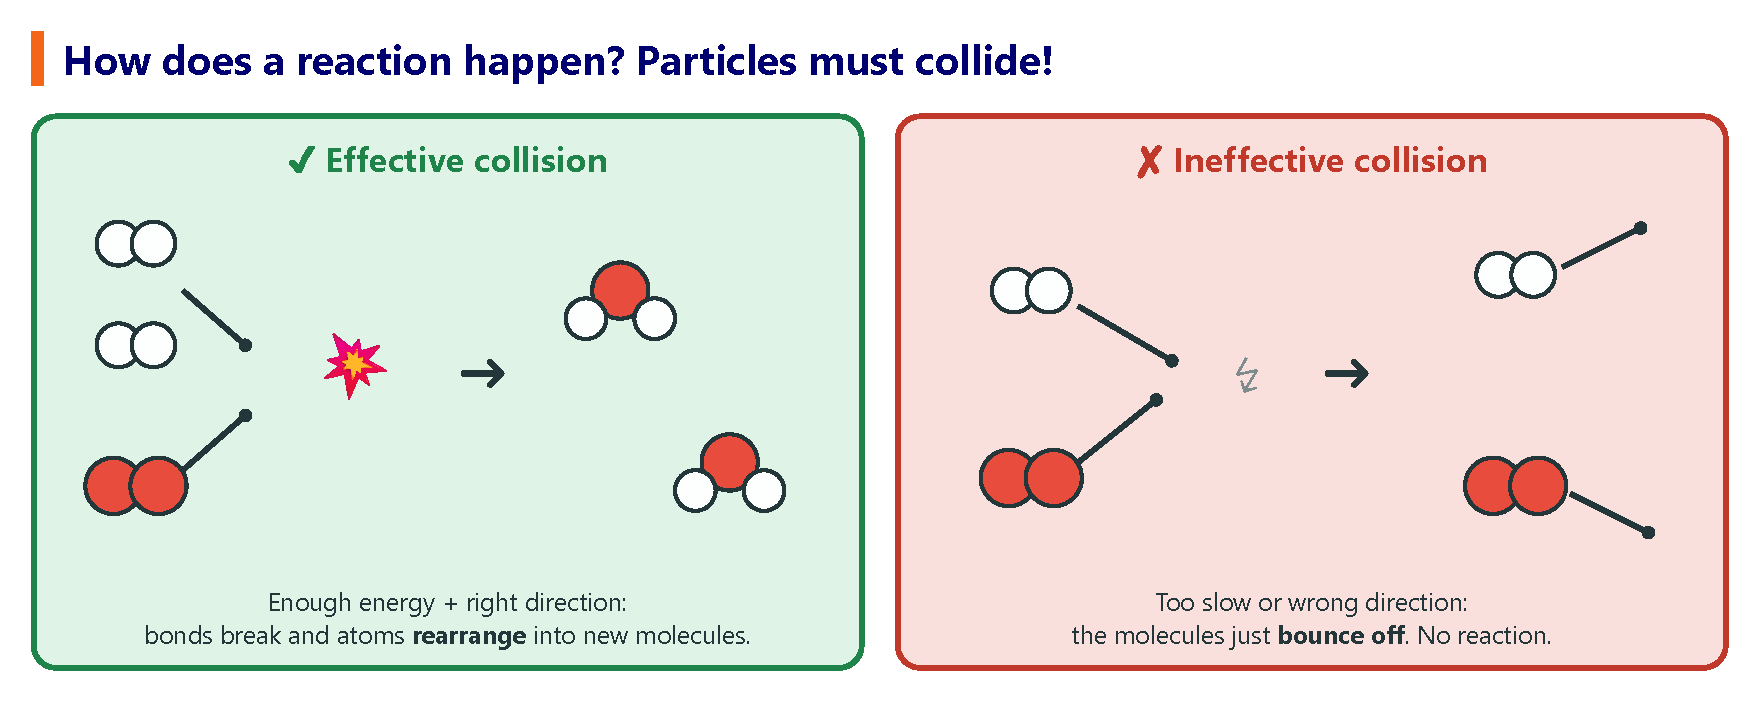
\includegraphics[width=\textwidth]{FigurasSVG/Unit_6_Chemical_Reactions/pdf/collisions.pdf}
    \caption{Only effective collisions produce a reaction: \(2\ch{H2} + \ch{O2} \longrightarrow 2\ch{H2O}\).}
    \label{fig:u6_collisions}
\end{figure}

\begin{exercise}
    Hydrogen and oxygen molecules are inside a container. In collision A, the molecules hit each other very gently; in collision B, they hit each other fast and head-on. In which case is a reaction more likely? Why?
    \begin{solu}
        In \textbf{collision B}. An effective collision needs \textbf{enough energy} and the right orientation. In collision A the molecules hit too gently, so their bonds do not break and they simply bounce off.
    \end{solu}
\end{exercise}

\begin{exercise}
    Hydrogen peroxide (\ch{H2O2}) can be formed from hydrogen (\ch{H2}) and oxygen (\ch{O2}).
    \begin{enumerate}[label=\letraminuscula]
        \item Identify the reactants and the products.
        \item Which are simple substances and which is a compound?
    \end{enumerate}
    \begin{solu}
        \begin{enumerate}[label=\alph*)]
            \item Reactants: \ch{H2} and \ch{O2}. Product: \ch{H2O2}.
            \item \ch{H2} and \ch{O2} are \textbf{simple substances}; \ch{H2O2} is a \textbf{compound}.
        \end{enumerate}
    \end{solu}
\end{exercise}

\begin{exercise}
    True or false? Correct the false statements.
    \begin{enumerate}[label=\letraminuscula]
        \item Every collision between reactant particles produces a chemical reaction.
        \item An effective collision needs enough energy and the correct orientation.
        \item Products are formed when the bonds of the reactants break and the atoms rearrange.
    \end{enumerate}
    \begin{solu}
        \begin{enumerate}[label=\alph*)]
            \item \textbf{False}: only \textit{effective} collisions produce a reaction.
            \item \textbf{True}.
            \item \textbf{True}.
        \end{enumerate}
    \end{solu}
\end{exercise}

\subsection{Chemical equations and the law of conservation of mass}

\begin{definition}[Chemical equation]
    The way we write a reaction with chemical formulas: reactants on the left, products on the right, and an arrow between them.
    \begin{equation*}
        \underbrace{\ch{N2} + 3\ch{H2}}_{\text{reactants}} \longrightarrow \underbrace{2\ch{NH3}}_{\text{products}}
    \end{equation*}
\end{definition}

\begin{figure}[H]
    \centering
    % [FIGURA ORIGINAL] \includegraphics[width=\textwidth]{Unit_6/conservation_mass}
    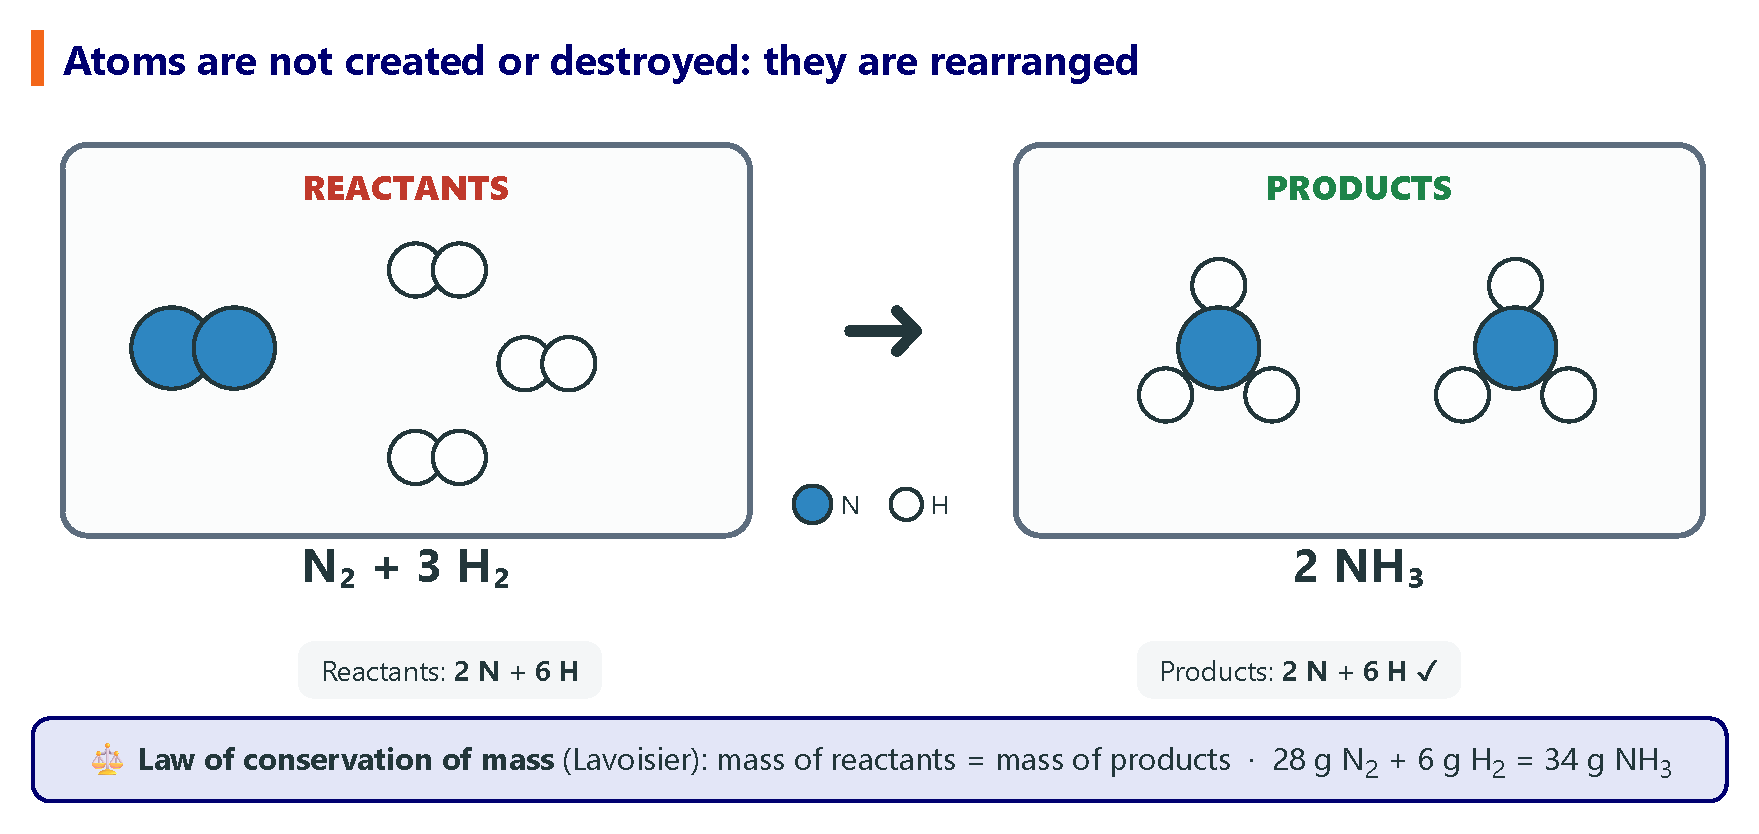
\includegraphics[width=\textwidth]{FigurasSVG/Unit_6_Chemical_Reactions/pdf/conservation_mass.pdf}
    \caption{The same atoms before and after: only the way they are joined changes.}
    \label{fig:u6_conservation_mass}
\end{figure}

\begin{definition}[Law of conservation of mass]
    In a chemical reaction, the total mass of the reactants is \textbf{equal} to the total mass of the products. Matter is not created or destroyed, only transformed (Lavoisier, 18th century).
\end{definition}

\begin{didyouknow}
    Antoine Lavoisier, the ``father of modern chemistry'', weighed everything very carefully in closed containers, which is how he discovered the law of conservation of mass. His famous sentence was: ``\emph{Nothing is lost, nothing is created, everything is transformed}''.
\end{didyouknow}

\begin{example}
    \textbf{Worked example: using the law of conservation of mass step by step.} When limestone (calcium carbonate, \ch{CaCO3}) is heated strongly, it decomposes into quicklime (calcium oxide, \ch{CaO}) and carbon dioxide gas (\ch{CO2}). We heat \qty{50}{\g} of calcium carbonate in a closed container until it has all reacted, and we obtain \qty{28}{\g} of calcium oxide. What mass of carbon dioxide has been formed?
    \begin{enumerate}[label=\numberballmDarkTeal]
        \item \textbf{Identify the reactants and the products.} The reactant is calcium carbonate; the products are calcium oxide and carbon dioxide:
        \[
            \ch{CaCO3} \longrightarrow \ch{CaO} + \ch{CO2}
        \]
        \item \textbf{Write down the data and the unknown.} \(m(\ch{CaCO3}) = \qty{50}{\g}\); \quad \(m(\ch{CaO}) = \qty{28}{\g}\); \quad \(m(\ch{CO2}) = \ ?\)
        \item \textbf{Apply the law of conservation of mass.} The total mass of the reactants is equal to the total mass of the products:
        \[
            m(\ch{CaCO3}) = m(\ch{CaO}) + m(\ch{CO2})
        \]
        \item \textbf{Substitute the data.}
        \[
            \qty{50}{\g} = \qty{28}{\g} + m(\ch{CO2})
        \]
        \item \textbf{Isolate the unknown.} The \qty{28}{\g} that are adding on the right go to the left subtracting:
        \[
            m(\ch{CO2}) = \qty{50}{\g} - \qty{28}{\g} = \textcolor{red}{\qty{22}{\g}}
        \]
        \item \textbf{Check the result.} Reactants: \qty{50}{\g}. Products: \(\qty{28}{\g} + \qty{22}{\g} = \qty{50}{\g}\). The masses are equal, so the answer is correct.
    \end{enumerate}
    \textbf{Why a closed container?} If we heat the limestone in an open container, the \ch{CO2} escapes into the air and the balance shows only \qty{28}{\g} at the end: it \emph{seems} that \qty{22}{\g} have been lost. The mass has not disappeared; it has simply left as a gas. That is why Lavoisier always weighed his reactions in closed containers.
\end{example}

\begin{exercise}
    \qty{4}{\g} of hydrogen react completely with \qty{32}{\g} of oxygen, forming water. What mass of water is obtained?
    \begin{solu}
        \(m(\ch{H2O}) = m(\ch{H2}) + m(\ch{O2}) = \qty{4}{\g} + \qty{32}{\g} = \qty{36}{\g}\).
    \end{solu}
\end{exercise}

\begin{exercise}
    \qty{5.6}{\g} of iron react completely with sulphur, giving \qty{8.8}{\g} of iron sulphide (\ch{FeS}). What mass of sulphur reacted?
    \begin{solu}
        \(m(\ch{S}) = m(\ch{FeS}) - m(\ch{Fe}) = \qty{8.8}{\g} - \qty{5.6}{\g} = \qty{3.2}{\g}\).
    \end{solu}
\end{exercise}

\begin{exercise}
    \qty{16}{\g} of methane (\ch{CH4}) burn completely with \qty{64}{\g} of oxygen, producing \qty{44}{\g} of carbon dioxide and some water vapour. What mass of water vapour is produced?
    \begin{solu}
        \(m(\ch{CH4}) + m(\ch{O2}) = m(\ch{CO2}) + m(\ch{H2O})\) \\
        \(\qty{16}{\g} + \qty{64}{\g} = \qty{44}{\g} + m(\ch{H2O}) \;\to\; m(\ch{H2O}) = \qty{36}{\g}\).
    \end{solu}
\end{exercise}

\subsection{Balancing chemical equations}

% Marks for the balancing tables: element balanced / not balanced
\providecommand{\balok}{\textcolor{green!50!black}{\(\checkmark\)}}
\providecommand{\balno}{\textcolor{red}{\(\boldsymbol{\times}\)}}

Balancing a chemical equation is one of the most important skills in chemistry. Atoms are not created or destroyed in a reaction (law of conservation of mass), so the equation must show \textbf{the same atoms} before and after the reaction.

\begin{definition}[Balanced chemical equation]
    A chemical equation that has the \textbf{same number of atoms of each element} on the reactants side (left) and on the products side (right).
\end{definition}

\begin{impt}
    \negsubro{The three basic rules}
    \begin{enumerate}[label=\numberballmDarkTeal]
        \item In the \textbf{reactants} there must be the \textbf{same number of atoms of each element} as in the \textbf{products}.
        \item We \textbf{count} the atoms of each element, one element at a time, in the reactants (\textbf{left}) and in the products (\textbf{right}).
        \item To make it easier, it is \textbf{advisable} to leave \textbf{hydrogen} and \textbf{oxygen} until the \textbf{end}, and oxygen the very last.
    \end{enumerate}
\end{impt}

\subsubsection{Stoichiometric coefficients}

To balance an equation we can only write numbers \textbf{in front of} the formulas. These numbers are called \negsubro{stoichiometric coefficients}.

\begin{definition}[Stoichiometric coefficient]
    A whole number (1, 2, 3\ldots) written \textbf{in front of} a formula in a chemical equation. It \textbf{multiplies} all the atoms of that formula. A coefficient of 1 is not written.
\end{definition}

\begin{figure}[H]
    \centering
    % [FIGURA ORIGINAL] \includegraphics[width=\textwidth]{Unit_6/coefficient_subscript}
    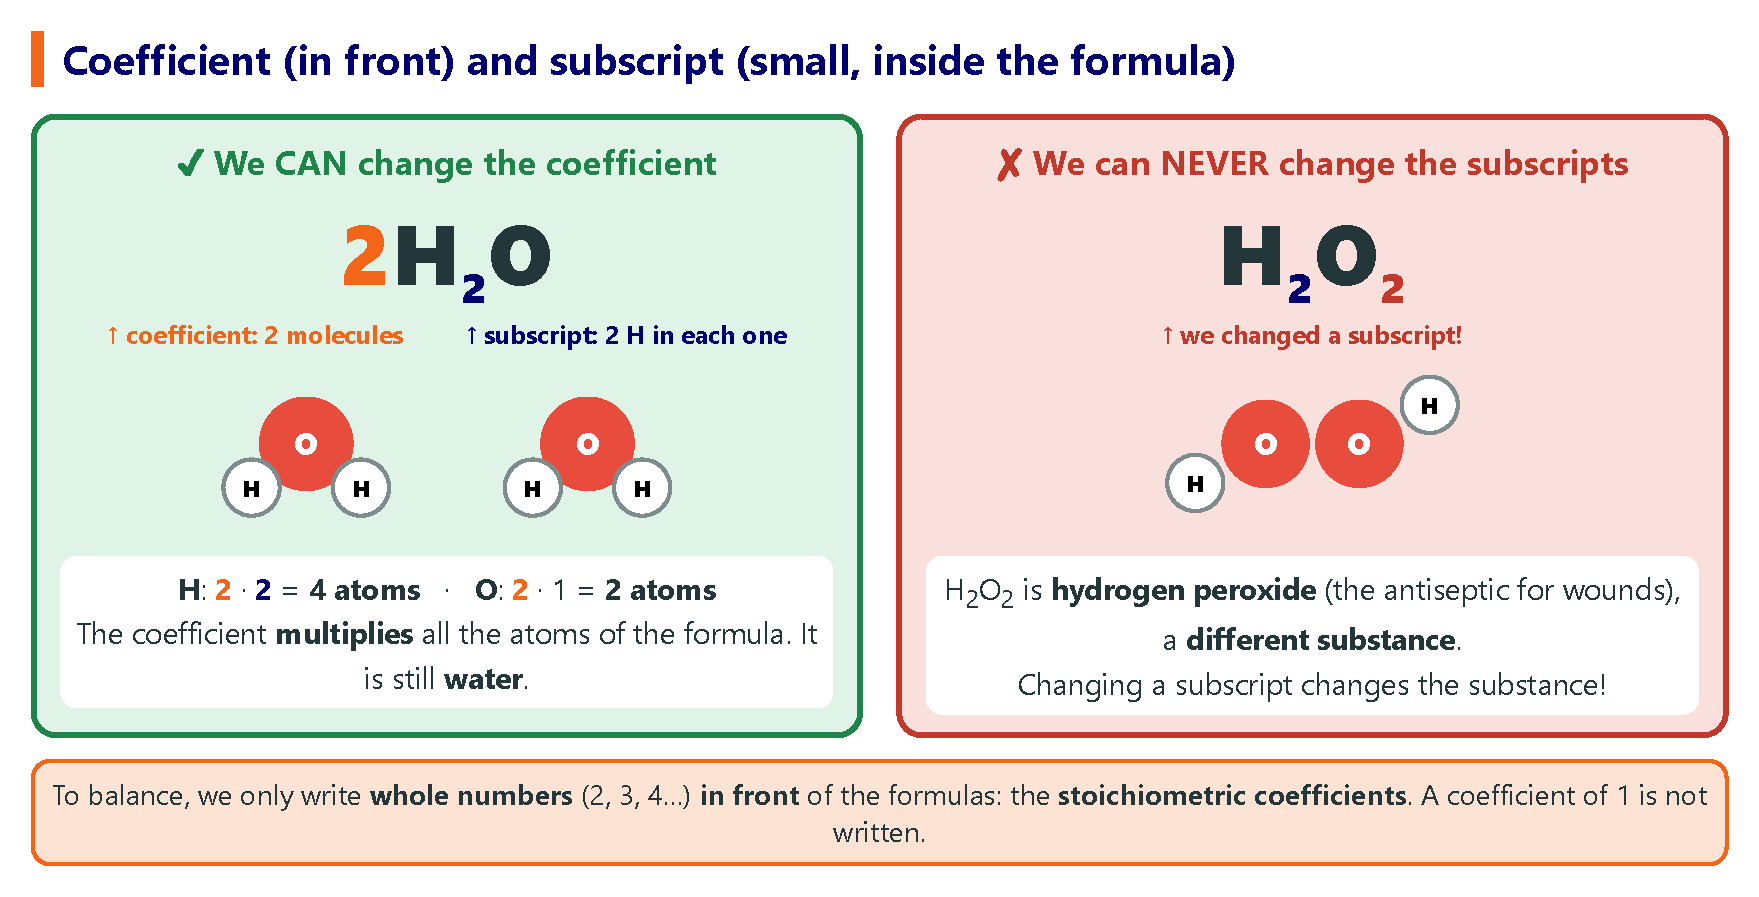
\includegraphics[width=\textwidth]{FigurasSVG/Unit_6_Chemical_Reactions/pdf/coefficient_subscript.pdf}
    \caption{The coefficient multiplies the whole formula; the subscripts can never be changed.}
    \label{fig:u6_coefficient_subscript}
\end{figure}

\begin{marker}
    \begin{itemize}
        \item The coefficients are written \textbf{in front} of the formula and \textbf{NEVER as a subscript}. If we change a subscript, we change the substance: \ch{H2O} is water, but \ch{H2O2} is hydrogen peroxide.
        \item Once we write a coefficient, it \textbf{multiplies the subscripts} of all the elements of that formula, so the number of atoms of \textbf{every} element in the formula changes: in \(3\ch{CO2}\) there are \(3 \cdot 1 = 3\) C and \(3 \cdot 2 = 6\) O.
        \item The coefficients must always be \textbf{whole numbers}: 1, 2, 3\ldots{} (never 1,5 or \(\frac{1}{2}\)).
    \end{itemize}
\end{marker}

\subsubsection{The method, step by step}

\begin{enumerate}[label=\numberballmDarkTeal]
    \item Write the equation and, \textbf{below it, a table}: one row for each element, and under each formula the number of atoms of that element. Add a column with the total on the left and another with the total on the right.
    \item Take the elements one by one: first the metals and the other elements, then \textbf{hydrogen} and finally \textbf{oxygen}.
    \item For each element, compare the total on the left with the total on the right:
    \begin{itemize}
        \item If they are \textbf{the same}, the element is balanced. We \textbf{keep} the coefficients and go on to the next element.
        \item If they are \textbf{different}, we go to the side with \textbf{fewer} atoms of that element and write in front of the formula that contains it a coefficient \textbf{one unit bigger} (if there is no number, it is a 1, so we write a 2). We \textbf{count again}. If the two sides are still different, we again increase by one the coefficient on the side that \textbf{now} has fewer atoms, and repeat until both sides are equal.
    \end{itemize}
    \item \textbf{Be careful}: when we write a coefficient, we also change the other elements of that formula. So, every time we balance a new element, we must \textbf{check again} that the elements we had already balanced are still balanced. If one is not, we balance it again.
    \item When \textbf{all} the elements are balanced, the equation is balanced. If all the coefficients can be divided by the same number, we simplify them (\(2, 4, 2 \to 1, 2, 1\)).
\end{enumerate}

\begin{figure}[H]
    \centering
    % [FIGURA ORIGINAL] \includegraphics[width=0.95\textwidth]{Unit_6/balancing_method}
    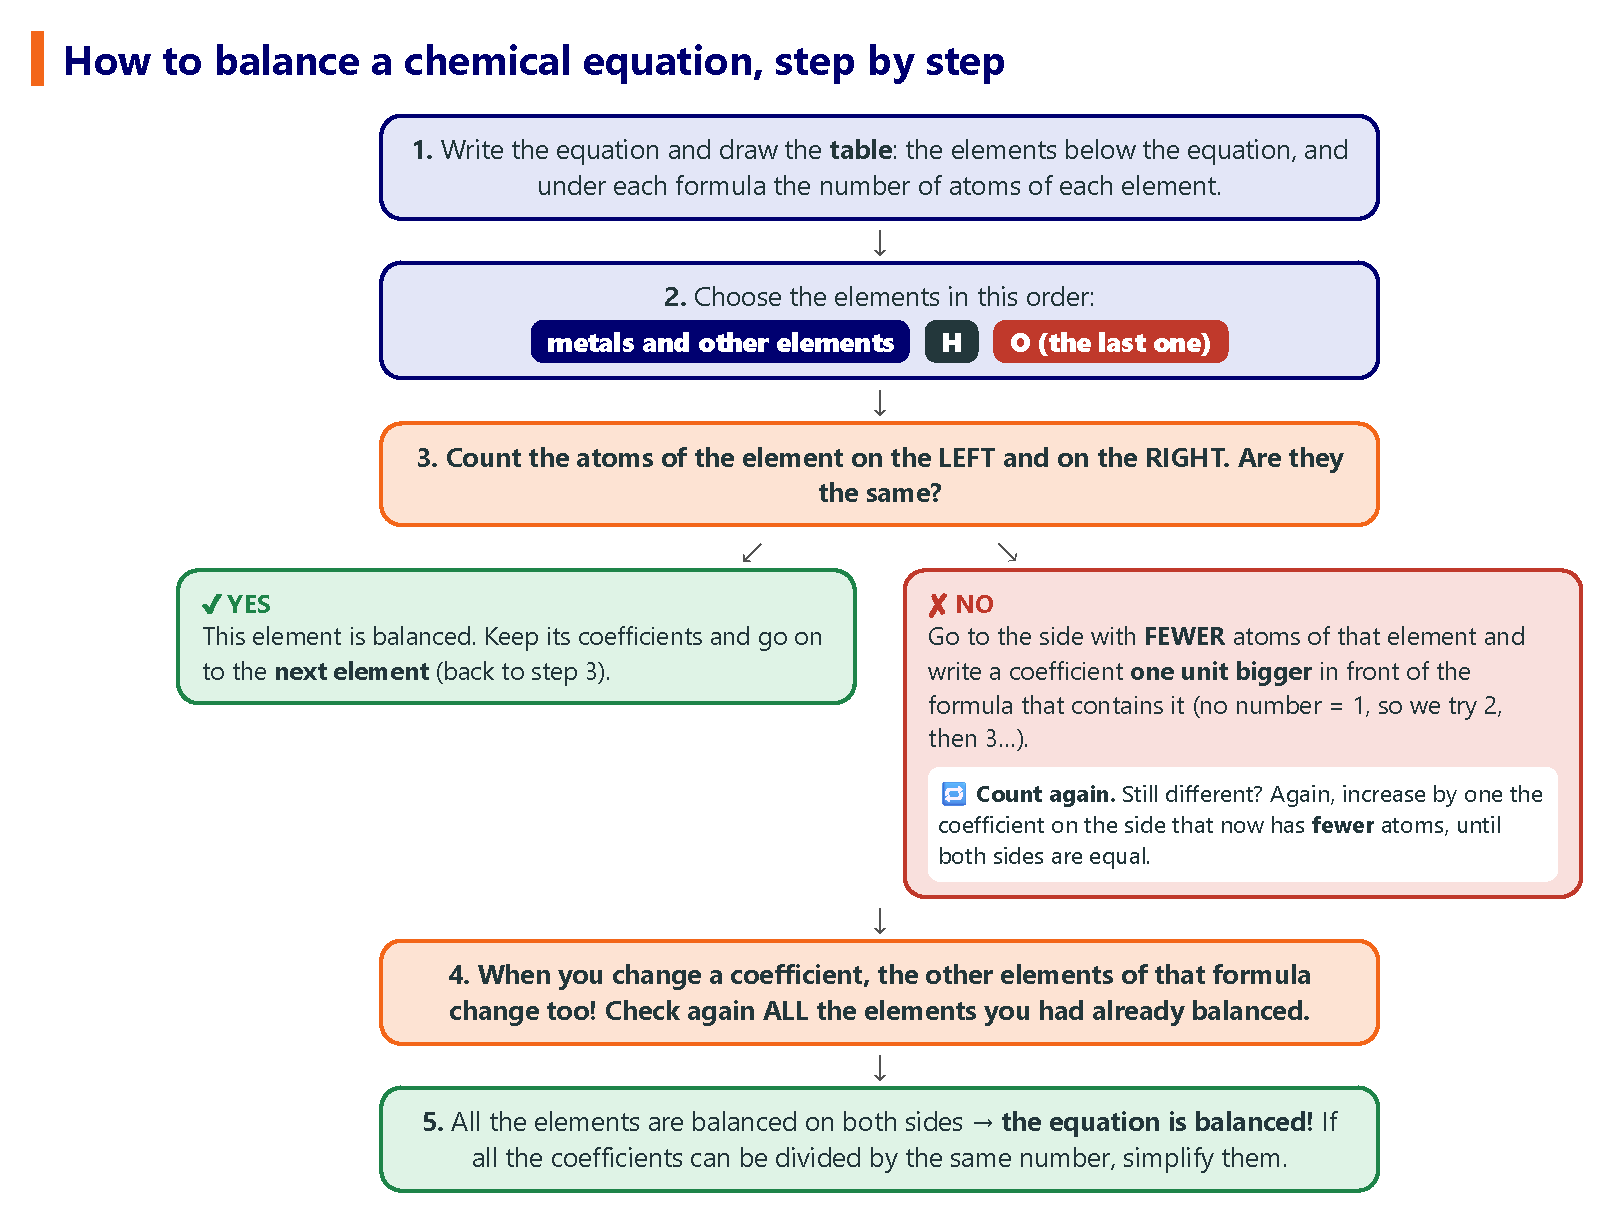
\includegraphics[width=0.95\textwidth]{FigurasSVG/Unit_6_Chemical_Reactions/pdf/balancing_method.pdf}
    \caption{The method for balancing a chemical equation.}
    \label{fig:u6_balancing_method}
\end{figure}

\begin{impt}
    \negsubro{The balancing table}: below the equation we write the elements, and under each formula the number of atoms of each element. When a formula has a coefficient, we multiply: coefficient \(\cdot\) subscript. The columns \textbf{Left} and \textbf{Right} show the totals, and the last column tells us whether that element is balanced (\balok) or not (\balno). The row of the element we are working on is \colorbox{yellow!25}{highlighted}, and the coefficient we have just written is in \textcolor{red}{\textbf{red}}.
\end{impt}

\begin{example}
    \textbf{Balance the equation for the formation of ammonia: } \(\ch{N2} + \ch{H2} \longrightarrow \ch{NH3}\)
\end{example}

\negsubro{Step 1}: we draw the table and count the atoms of each element.
\begin{center}
    \small\renewcommand{\arraystretch}{1.3}
    % --- tabla antigua ---
    % \begin{tabular}{l|cc|>{\columncolor{blue!8}}c||c|>{\columncolor{blue!8}}c|c}
        % \textbf{Element} & \ch{N2} & \ch{H2} & \textbf{Left} & \ch{NH3} & \textbf{Right} &  \\
        % \hline
        % \textbf{N} & 2 & -- & \textbf{2} & 1 & \textbf{1} & \balno \\
        % \textbf{H} & -- & 2 & \textbf{2} & 3 & \textbf{3} & \balno \\
    % \end{tabular}
    % --- tabla nueva ---
    \begin{tabular}{@{}lcccccc@{}}
        \toprule
        \textbf{Element} & \textbf{\ch{N2}} & \textbf{\ch{H2}} & \textbf{Left} & \textbf{\ch{NH3}} & \textbf{Right} &  \\
        \midrule
        \textbf{N} & 2 & -- & \textbf{2} & 1 & \textbf{1} & \balno \\[3pt]
        \textbf{H} & -- & 2 & \textbf{2} & 3 & \textbf{3} & \balno \\
        \bottomrule
    \end{tabular}
\end{center}

\negsubro{Step 2: nitrogen.} On the left there are 2 N and on the right only 1 N. The \textbf{right} side has fewer, so we write a \textbf{2} in front of \ch{NH3}. Now we count again: \(2 \cdot 1 = 2\) N on the right. \balok{} Notice that the H on the right have also changed: \(2 \cdot 3 = 6\).
\begin{center}
    \small\renewcommand{\arraystretch}{1.3}
    % --- tabla antigua ---
    % \begin{tabular}{l|cc|>{\columncolor{blue!8}}c||c|>{\columncolor{blue!8}}c|c}
        % \textbf{Element} & \ch{N2} & \ch{H2} & \textbf{Left} & \textcolor{red}{\textbf{2}}\ch{NH3} & \textbf{Right} &  \\
        % \hline
        % \rowcolor{yellow!25} \textbf{N} & 2 & -- & \textbf{2} & \(2 \cdot 1 = 2\) & \textbf{2} & \balok \\
        % \textbf{H} & -- & 2 & \textbf{2} & \(2 \cdot 3 = 6\) & \textbf{6} & \balno \\
    % \end{tabular}
    % --- tabla nueva ---
    \begin{tabular}{@{}lcccccc@{}}
        \toprule
        \textbf{Element} & \textbf{\ch{N2}} & \textbf{\ch{H2}} & \textbf{Left} & \textcolor{red}{\textbf{2}}\ch{NH3} & \textbf{Right} &  \\
        \midrule
        \textbf{N} & 2 & -- & \textbf{2} & \(2 \cdot 1 = 2\) & \textbf{2} & \balok \\[3pt]
        \textbf{H} & -- & 2 & \textbf{2} & \(2 \cdot 3 = 6\) & \textbf{6} & \balno \\
        \bottomrule
    \end{tabular}
\end{center}
\negsubro{Step 3: hydrogen.} On the left there are 2 H and on the right 6 H. The \textbf{left} side has fewer, so we increase the coefficient of \ch{H2} one unit at a time: with a 2 we get \(2 \cdot 2 = 4\) H \balno; with a 3 we get \(3 \cdot 2 = 6\) H \balok.
\begin{center}
    \small\renewcommand{\arraystretch}{1.3}
    % --- tabla antigua ---
    % \begin{tabular}{l|cc|>{\columncolor{blue!8}}c||c|>{\columncolor{blue!8}}c|c}
        % \textbf{Element} & \ch{N2} & \textcolor{red}{\textbf{3}}\ch{H2} & \textbf{Left} & 2\ch{NH3} & \textbf{Right} &  \\
        % \hline
        % \textbf{N} & 2 & -- & \textbf{2} & \(2 \cdot 1 = 2\) & \textbf{2} & \balok \\
        % \rowcolor{yellow!25} \textbf{H} & -- & \(3 \cdot 2 = 6\) & \textbf{6} & \(2 \cdot 3 = 6\) & \textbf{6} & \balok \\
    % \end{tabular}
    % --- tabla nueva ---
    \begin{tabular}{@{}lcccccc@{}}
        \toprule
        \textbf{Element} & \textbf{\ch{N2}} & \textcolor{red}{\textbf{3}}\ch{H2} & \textbf{Left} & \textbf{2\ch{NH3}} & \textbf{Right} &  \\
        \midrule
        \textbf{N} & 2 & -- & \textbf{2} & \(2 \cdot 1 = 2\) & \textbf{2} & \balok \\[3pt]
        \textbf{H} & -- & \(3 \cdot 2 = 6\) & \textbf{6} & \(2 \cdot 3 = 6\) & \textbf{6} & \balok \\
        \bottomrule
    \end{tabular}
\end{center}
\negsubro{Step 4: check.} The nitrogen is still balanced (2 = 2) and the hydrogen too (6 = 6). The balanced equation is:
\begin{equation*}
    \ch{N2} + 3\ch{H2} \longrightarrow 2\ch{NH3}
\end{equation*}

\begin{example}
    \textbf{Balance the combustion of methane (natural gas): } \(\ch{CH4} + \ch{O2} \longrightarrow \ch{CO2} + \ch{H2O}\)
\end{example}

\negsubro{Step 1}: the table. We will leave H and O for the end, and O the very last.
\begin{center}
    \small\renewcommand{\arraystretch}{1.3}
    % --- tabla antigua ---
    % \begin{tabular}{l|cc|>{\columncolor{blue!8}}c||cc|>{\columncolor{blue!8}}c|c}
        % \textbf{Element} & \ch{CH4} & \ch{O2} & \textbf{Left} & \ch{CO2} & \ch{H2O} & \textbf{Right} &  \\
        % \hline
        % \textbf{C} & 1 & -- & \textbf{1} & 1 & -- & \textbf{1} & \balok \\
        % \textbf{H} & 4 & -- & \textbf{4} & -- & 2 & \textbf{2} & \balno \\
        % \textbf{O} & -- & 2 & \textbf{2} & 2 & 1 & \textbf{3} & \balno \\
    % \end{tabular}
    % --- tabla nueva ---
    \begin{tabular}{@{}lccccccc@{}}
        \toprule
        \textbf{Element} & \textbf{\ch{CH4}} & \textbf{\ch{O2}} & \textbf{Left} & \textbf{\ch{CO2}} & \textbf{\ch{H2O}} & \textbf{Right} &  \\
        \midrule
        \textbf{C} & 1 & -- & \textbf{1} & 1 & -- & \textbf{1} & \balok \\[3pt]
        \textbf{H} & 4 & -- & \textbf{4} & -- & 2 & \textbf{2} & \balno \\[3pt]
        \textbf{O} & -- & 2 & \textbf{2} & 2 & 1 & \textbf{3} & \balno \\
        \bottomrule
    \end{tabular}
\end{center}

\negsubro{Step 2: carbon.} 1 C on the left and 1 C on the right. \balok{} We go on to the next element.

\negsubro{Step 3: hydrogen.} 4 H on the left and 2 H on the right. The \textbf{right} side has fewer, so we write a \textbf{2} in front of \ch{H2O}: \(2 \cdot 2 = 4\) H. \balok
\begin{center}
    \small\renewcommand{\arraystretch}{1.3}
    % --- tabla antigua ---
    % \begin{tabular}{l|cc|>{\columncolor{blue!8}}c||cc|>{\columncolor{blue!8}}c|c}
        % \textbf{Element} & \ch{CH4} & \ch{O2} & \textbf{Left} & \ch{CO2} & \textcolor{red}{\textbf{2}}\ch{H2O} & \textbf{Right} &  \\
        % \hline
        % \textbf{C} & 1 & -- & \textbf{1} & 1 & -- & \textbf{1} & \balok \\
        % \rowcolor{yellow!25} \textbf{H} & 4 & -- & \textbf{4} & -- & \(2 \cdot 2 = 4\) & \textbf{4} & \balok \\
        % \textbf{O} & -- & 2 & \textbf{2} & 2 & \(2 \cdot 1 = 2\) & \textbf{4} & \balno \\
    % \end{tabular}
    % --- tabla nueva ---
    \begin{tabular}{@{}lccccccc@{}}
        \toprule
        \textbf{Element} & \textbf{\ch{CH4}} & \textbf{\ch{O2}} & \textbf{Left} & \textbf{\ch{CO2}} & \textcolor{red}{\textbf{2}}\ch{H2O} & \textbf{Right} &  \\
        \midrule
        \textbf{C} & 1 & -- & \textbf{1} & 1 & -- & \textbf{1} & \balok \\[3pt]
        \textbf{H} & 4 & -- & \textbf{4} & -- & \(2 \cdot 2 = 4\) & \textbf{4} & \balok \\[3pt]
        \textbf{O} & -- & 2 & \textbf{2} & 2 & \(2 \cdot 1 = 2\) & \textbf{4} & \balno \\
        \bottomrule
    \end{tabular}
\end{center}
\negsubro{Step 4: oxygen (the last one).} On the left there are 2 O; on the right, \(2 + 2 = 4\) O (2 in \ch{CO2} and 2 in \(2\ch{H2O}\)). The \textbf{left} side has fewer, so we write a \textbf{2} in front of \ch{O2}: \(2 \cdot 2 = 4\) O. \balok
\begin{center}
    \small\renewcommand{\arraystretch}{1.3}
    % --- tabla antigua ---
    % \begin{tabular}{l|cc|>{\columncolor{blue!8}}c||cc|>{\columncolor{blue!8}}c|c}
        % \textbf{Element} & \ch{CH4} & \textcolor{red}{\textbf{2}}\ch{O2} & \textbf{Left} & \ch{CO2} & 2\ch{H2O} & \textbf{Right} &  \\
        % \hline
        % \textbf{C} & 1 & -- & \textbf{1} & 1 & -- & \textbf{1} & \balok \\
        % \textbf{H} & 4 & -- & \textbf{4} & -- & \(2 \cdot 2 = 4\) & \textbf{4} & \balok \\
        % \rowcolor{yellow!25} \textbf{O} & -- & \(2 \cdot 2 = 4\) & \textbf{4} & 2 & \(2 \cdot 1 = 2\) & \textbf{4} & \balok \\
    % \end{tabular}
    % --- tabla nueva ---
    \begin{tabular}{@{}lccccccc@{}}
        \toprule
        \textbf{Element} & \textbf{\ch{CH4}} & \textcolor{red}{\textbf{2}}\ch{O2} & \textbf{Left} & \textbf{\ch{CO2}} & \textbf{2\ch{H2O}} & \textbf{Right} &  \\
        \midrule
        \textbf{C} & 1 & -- & \textbf{1} & 1 & -- & \textbf{1} & \balok \\[3pt]
        \textbf{H} & 4 & -- & \textbf{4} & -- & \(2 \cdot 2 = 4\) & \textbf{4} & \balok \\[3pt]
        \textbf{O} & -- & \(2 \cdot 2 = 4\) & \textbf{4} & 2 & \(2 \cdot 1 = 2\) & \textbf{4} & \balok \\
        \bottomrule
    \end{tabular}
\end{center}
\negsubro{Step 5: check.} C: 1 = 1; H: 4 = 4; O: 4 = 4. The balanced equation is:
\begin{equation*}
    \ch{CH4} + 2\ch{O2} \longrightarrow \ch{CO2} + 2\ch{H2O}
\end{equation*}
Leaving oxygen for the end made it easy: \ch{O2} only contains oxygen, so changing its coefficient did not unbalance any other element.

\begin{example}
    \textbf{Balance the oxidation of aluminium: } \(\ch{Al} + \ch{O2} \longrightarrow \ch{Al2O3}\) \textbf{(a more difficult case)}
\end{example}

\negsubro{Step 1}: the table.
\begin{center}
    \small\renewcommand{\arraystretch}{1.3}
    % --- tabla antigua ---
    % \begin{tabular}{l|cc|>{\columncolor{blue!8}}c||c|>{\columncolor{blue!8}}c|c}
        % \textbf{Element} & \ch{Al} & \ch{O2} & \textbf{Left} & \ch{Al2O3} & \textbf{Right} &  \\
        % \hline
        % \textbf{Al} & 1 & -- & \textbf{1} & 2 & \textbf{2} & \balno \\
        % \textbf{O} & -- & 2 & \textbf{2} & 3 & \textbf{3} & \balno \\
    % \end{tabular}
    % --- tabla nueva ---
    \begin{tabular}{@{}lcccccc@{}}
        \toprule
        \textbf{Element} & \textbf{\ch{Al}} & \textbf{\ch{O2}} & \textbf{Left} & \textbf{\ch{Al2O3}} & \textbf{Right} &  \\
        \midrule
        \textbf{Al} & 1 & -- & \textbf{1} & 2 & \textbf{2} & \balno \\[3pt]
        \textbf{O} & -- & 2 & \textbf{2} & 3 & \textbf{3} & \balno \\
        \bottomrule
    \end{tabular}
\end{center}

\negsubro{Step 2: aluminium.} 1 Al on the left and 2 Al on the right. The \textbf{left} side has fewer: we write a \textbf{2} in front of \ch{Al}. \balok
\begin{center}
    \small\renewcommand{\arraystretch}{1.3}
    % --- tabla antigua ---
    % \begin{tabular}{l|cc|>{\columncolor{blue!8}}c||c|>{\columncolor{blue!8}}c|c}
        % \textbf{Element} & \textcolor{red}{\textbf{2}}\ch{Al} & \ch{O2} & \textbf{Left} & \ch{Al2O3} & \textbf{Right} &  \\
        % \hline
        % \rowcolor{yellow!25} \textbf{Al} & \(2 \cdot 1 = 2\) & -- & \textbf{2} & 2 & \textbf{2} & \balok \\
        % \textbf{O} & -- & 2 & \textbf{2} & 3 & \textbf{3} & \balno \\
    % \end{tabular}
    % --- tabla nueva ---
    \begin{tabular}{@{}lcccccc@{}}
        \toprule
        \textbf{Element} & \textcolor{red}{\textbf{2}}\ch{Al} & \textbf{\ch{O2}} & \textbf{Left} & \textbf{\ch{Al2O3}} & \textbf{Right} &  \\
        \midrule
        \textbf{Al} & \(2 \cdot 1 = 2\) & -- & \textbf{2} & 2 & \textbf{2} & \balok \\[3pt]
        \textbf{O} & -- & 2 & \textbf{2} & 3 & \textbf{3} & \balno \\
        \bottomrule
    \end{tabular}
\end{center}
\negsubro{Step 3: oxygen.} 2 O on the left and 3 O on the right. Each time, we increase by one the coefficient on the side that has \textbf{fewer} atoms at that moment:
\begin{itemize}
    \item The left has fewer (2 < 3): \(2\ch{O2}\) \(\to\) 4 O on the left. Now \(4 > 3\) \balno
    \item Now the right has fewer (3 < 4): \(2\ch{Al2O3}\) \(\to\) \(2 \cdot 3 = 6\) O on the right. \(4 < 6\) \balno
    \item The left has fewer again (4 < 6): \(3\ch{O2}\) \(\to\) \(3 \cdot 2 = 6\) O. \(6 = 6\) \balok
\end{itemize}
\begin{center}
    \small\renewcommand{\arraystretch}{1.3}
    % --- tabla antigua ---
    % \begin{tabular}{l|cc|>{\columncolor{blue!8}}c||c|>{\columncolor{blue!8}}c|c}
        % \textbf{Element} & 2\ch{Al} & \textcolor{red}{\textbf{3}}\ch{O2} & \textbf{Left} & 2\ch{Al2O3} & \textbf{Right} &  \\
        % \hline
        % \textbf{Al} & \(2 \cdot 1 = 2\) & -- & \textbf{2} & \(2 \cdot 2 = 4\) & \textbf{4} & \balno \\
        % \rowcolor{yellow!25} \textbf{O} & -- & \(3 \cdot 2 = 6\) & \textbf{6} & \(2 \cdot 3 = 6\) & \textbf{6} & \balok \\
    % \end{tabular}
    % --- tabla nueva ---
    \begin{tabular}{@{}lcccccc@{}}
        \toprule
        \textbf{Element} & \textbf{2\ch{Al}} & \textcolor{red}{\textbf{3}}\ch{O2} & \textbf{Left} & \textbf{2\ch{Al2O3}} & \textbf{Right} &  \\
        \midrule
        \textbf{Al} & \(2 \cdot 1 = 2\) & -- & \textbf{2} & \(2 \cdot 2 = 4\) & \textbf{4} & \balno \\[3pt]
        \textbf{O} & -- & \(3 \cdot 2 = 6\) & \textbf{6} & \(2 \cdot 3 = 6\) & \textbf{6} & \balok \\
        \bottomrule
    \end{tabular}
\end{center}
\negsubro{Step 4: check the elements we had already balanced!} When we wrote the 2 in front of \ch{Al2O3}, the aluminium on the right changed: now there are \(2 \cdot 2 = 4\) Al on the right, but only 2 on the left. \balno{} The left has fewer: we try \(3\ch{Al}\) (3 Al \balno) and then \(4\ch{Al}\) (4 Al \balok).
\begin{center}
    \small\renewcommand{\arraystretch}{1.3}
    % --- tabla antigua ---
    % \begin{tabular}{l|cc|>{\columncolor{blue!8}}c||c|>{\columncolor{blue!8}}c|c}
        % \textbf{Element} & \textcolor{red}{\textbf{4}}\ch{Al} & 3\ch{O2} & \textbf{Left} & 2\ch{Al2O3} & \textbf{Right} &  \\
        % \hline
        % \rowcolor{yellow!25} \textbf{Al} & \(4 \cdot 1 = 4\) & -- & \textbf{4} & \(2 \cdot 2 = 4\) & \textbf{4} & \balok \\
        % \textbf{O} & -- & \(3 \cdot 2 = 6\) & \textbf{6} & \(2 \cdot 3 = 6\) & \textbf{6} & \balok \\
    % \end{tabular}
    % --- tabla nueva ---
    \begin{tabular}{@{}lcccccc@{}}
        \toprule
        \textbf{Element} & \textcolor{red}{\textbf{4}}\ch{Al} & \textbf{3\ch{O2}} & \textbf{Left} & \textbf{2\ch{Al2O3}} & \textbf{Right} &  \\
        \midrule
        \textbf{Al} & \(4 \cdot 1 = 4\) & -- & \textbf{4} & \(2 \cdot 2 = 4\) & \textbf{4} & \balok \\[3pt]
        \textbf{O} & -- & \(3 \cdot 2 = 6\) & \textbf{6} & \(2 \cdot 3 = 6\) & \textbf{6} & \balok \\
        \bottomrule
    \end{tabular}
\end{center}
\negsubro{Step 5: final check.} Al: 4 = 4; O: 6 = 6. The balanced equation is:
\begin{equation*}
    4\ch{Al} + 3\ch{O2} \longrightarrow 2\ch{Al2O3}
\end{equation*}

\begin{exercise}
    Balance these chemical equations:
    \begin{enumerate}[label=\letraminuscula]
        \item \(\ch{Mg} + \ch{O2} \longrightarrow \ch{MgO}\)
        \item \(\ch{Fe} + \ch{HCl} \longrightarrow \ch{FeCl2} + \ch{H2}\)
        \item \(\ch{C3H8} + \ch{O2} \longrightarrow \ch{CO2} + \ch{H2O}\)
    \end{enumerate}
    \begin{solu}
        \begin{enumerate}[label=\alph*)]
            \item \(2\ch{Mg} + \ch{O2} \longrightarrow 2\ch{MgO}\)
            \item \(\ch{Fe} + 2\ch{HCl} \longrightarrow \ch{FeCl2} + \ch{H2}\)
            \item \(\ch{C3H8} + 5\ch{O2} \longrightarrow 3\ch{CO2} + 4\ch{H2O}\)
        \end{enumerate}
    \end{solu}
\end{exercise}

\begin{exercise}
    Balance these chemical equations:
    \begin{enumerate}[label=\letraminuscula]
        \item \(\ch{Al} + \ch{O2} \longrightarrow \ch{Al2O3}\)
        \item \(\ch{CH4} + \ch{O2} \longrightarrow \ch{CO2} + \ch{H2O}\)
        \item \(\ch{Na} + \ch{Cl2} \longrightarrow \ch{NaCl}\)
    \end{enumerate}
    \begin{solu}
        \begin{enumerate}[label=\alph*)]
            \item \(4\ch{Al} + 3\ch{O2} \longrightarrow 2\ch{Al2O3}\)
            \item \(\ch{CH4} + 2\ch{O2} \longrightarrow \ch{CO2} + 2\ch{H2O}\)
            \item \(2\ch{Na} + \ch{Cl2} \longrightarrow 2\ch{NaCl}\)
        \end{enumerate}
    \end{solu}
\end{exercise}

\begin{exercise}
    Balance these chemical equations, using the balancing table:
    \begin{enumerate}[label=\letraminuscula]
        \item \(\ch{H2} + \ch{O2} \longrightarrow \ch{H2O}\)
        \item \(\ch{Zn} + \ch{HCl} \longrightarrow \ch{ZnCl2} + \ch{H2}\)
        \item \(\ch{KClO3} \longrightarrow \ch{KCl} + \ch{O2}\)
        \item \(\ch{Fe} + \ch{O2} \longrightarrow \ch{Fe2O3}\)
        \item \(\ch{C2H4} + \ch{O2} \longrightarrow \ch{CO2} + \ch{H2O}\)
    \end{enumerate}
    \begin{solu}
        \begin{enumerate}[label=\alph*)]
            \item \(2\ch{H2} + \ch{O2} \longrightarrow 2\ch{H2O}\)
            \item \(\ch{Zn} + 2\ch{HCl} \longrightarrow \ch{ZnCl2} + \ch{H2}\)
            \item \(2\ch{KClO3} \longrightarrow 2\ch{KCl} + 3\ch{O2}\)
            \item \(4\ch{Fe} + 3\ch{O2} \longrightarrow 2\ch{Fe2O3}\)
            \item \(\ch{C2H4} + 3\ch{O2} \longrightarrow 2\ch{CO2} + 2\ch{H2O}\)
        \end{enumerate}
    \end{solu}
\end{exercise}

%\subsection{Important chemical reactions}
%
%\begin{figure}[H]
%    \centering
%    \includegraphics[width=\textwidth]{Unit_6/important_reactions}
%    \caption{Some chemical reactions that are very important in our lives.}
%    \label{fig:u6_important_reactions}
%\end{figure}
%
%\begin{figure}[H]
%    \centering
%    \includegraphics[width=0.95\textwidth]{Unit_6/life_reactions}
%    \caption{Photosynthesis and cellular respiration.}
%    \label{fig:u6_life_reactions}
%\end{figure}
%
%\begin{align*}
%    \text{Photosynthesis:} \quad & 6\ch{CO2} + 6\ch{H2O} + \text{light energy} \longrightarrow \ch{C6H12O6} + 6\ch{O2} \\
%    \text{Cellular respiration:} \quad & \ch{C6H12O6} + 6\ch{O2} \longrightarrow 6\ch{CO2} + 6\ch{H2O} + \text{energy}
%\end{align*}
%
%\begin{exercise}
%    Natural gas is used for cooking in many homes. Is the reaction that takes place when it burns an oxidation or a combustion?
%    \begin{solu}
%        A \textbf{combustion}: the gas reacts quickly with the oxygen in the air, releasing a lot of heat and light and producing \ch{CO2}. (A combustion is a fast type of oxidation.)
%    \end{solu}
%\end{exercise}
%
%\begin{exercise}
%    Stainless steel (iron with a little carbon and chromium) is used for kitchen utensils and outdoor objects.
%    \begin{enumerate}[label=\letraminuscula]
%        \item What type of mixture is steel?
%        \item Which chemical reaction does it help to prevent?
%    \end{enumerate}
%    \begin{solu}
%        \begin{enumerate}[label=\alph*)]
%            \item A \textbf{homogeneous mixture}: an alloy (a solid solution).
%            \item The \textbf{oxidation} (rusting) of iron.
%        \end{enumerate}
%    \end{solu}
%\end{exercise}
%
%\begin{exercise}
%    A person with stomach acidity takes an antacid tablet, which contains a base. What type of reaction takes place, and what types of products are formed?
%    \begin{solu}
%        A \textbf{neutralisation}: the base reacts with the excess acid, forming a \textbf{salt} and \textbf{water}.
%    \end{solu}
%\end{exercise}
%
%\begin{exercise}
%    Explain why photosynthesis and cellular respiration are opposite processes, both in terms of matter and of energy.
%    \begin{solu}
%        \textbf{Matter}: the reactants of photosynthesis (\ch{CO2} and \ch{H2O}) are the products of respiration, and the products of photosynthesis (glucose and \ch{O2}) are the reactants of respiration. \\
%        \textbf{Energy}: photosynthesis \textbf{absorbs} light energy and stores it in glucose; respiration \textbf{releases} that energy for living things.
%    \end{solu}
%\end{exercise}
%
%\begin{exercise}
%    Yeast is added to grape juice to make wine. Which type of reaction takes place? Name two products besides alcohol.
%    \begin{solu}
%        \textbf{Fermentation}. Besides alcohol (ethanol), it produces \textbf{carbon dioxide} and releases \textbf{energy}.
%    \end{solu}
%\end{exercise}
%
%\subsection{Chemical reactions, technology and society}
%
%\begin{figure}[H]
%    \centering
%    \includegraphics[width=\textwidth]{Unit_6/environment}
%    \caption{Chemical reactions bring benefits, but also environmental problems that chemistry helps to solve.}
%    \label{fig:u6_environment}
%\end{figure}
%
%\begin{exercise}
%    Explain why reducing car emissions \textbf{and} planting trees are both useful to fight climate change.
%    \begin{solu}
%        Car engines burn fuel (\textbf{combustion}), releasing \ch{CO2}; reducing emissions means less \ch{CO2} in the air. Trees take in \ch{CO2} during \textbf{photosynthesis}, so planting them removes \ch{CO2} from the atmosphere. Both reduce the amount of greenhouse gases.
%    \end{solu}
%\end{exercise}
%
%\begin{exercise}
%    Sulphur and nitrogen oxides react with water vapour in the atmosphere and form \negsubro{acid rain}. Which human activity releases most of them, and what measure could reduce them?
%    \begin{solu}
%        The \textbf{combustion} of fossil fuels in power plants, factories and vehicles. Possible measures: catalytic converters, cleaner fuels and renewable energy (goals of green chemistry).
%    \end{solu}
%\end{exercise}
%
%\begin{exercise}
%    Explain, using an example, how the same type of reaction can bring both benefits and problems.
%    \begin{solu}
%        \textbf{Combustion} gives us most of the energy for transport, heating and electricity, but it also releases \ch{CO2} (greenhouse effect) and other gases that cause acid rain.
%    \end{solu}
%\end{exercise}
%
%\subsection{How to change the speed of a reaction}
%
%\begin{figure}[H]
%    \centering
%    \includegraphics[width=\textwidth]{Unit_6/reaction_speed}
%    \caption{Four factors that change the speed of a reaction. The faster reaction reaches the same final amount of product sooner.}
%    \label{fig:u6_reaction_speed}
%\end{figure}
%
%\begin{definition}[Catalyst]
%    A substance that makes a reaction faster without being used up. The \textbf{enzymes} in our body are catalysts: they help us, for example, to digest food.
%\end{definition}
%
%\begin{exercise}
%    Which factor is used to change the speed of the reaction in each case? Apples are chopped to make jam; very dirty clothes are washed at a high temperature; dried fruit is sold vacuum-packed; enzymes are added to milk to make cheese.
%    \begin{solu}
%        Chopping apples: \textbf{contact area}. \\
%        Hot washing: \textbf{temperature}. \\
%        Vacuum packing: \textbf{concentration} (less oxygen, so slower oxidation). \\
%        Enzymes: \textbf{catalyst}.
%    \end{solu}
%\end{exercise}
%
%\begin{exercise}
%    A car's catalytic converter contains platinum, which speeds up the reaction that turns toxic carbon monoxide into carbon dioxide, without the platinum being used up.
%    \begin{enumerate}[label=\letraminuscula]
%        \item What does the platinum act as?
%        \item Why does it not need to be replaced after every journey?
%    \end{enumerate}
%    \begin{solu}
%        \begin{enumerate}[label=\alph*)]
%            \item A \textbf{catalyst}.
%            \item A catalyst is not used up in the reaction, so it can keep working again and again.
%        \end{enumerate}
%    \end{solu}
%\end{exercise}
%
%\begin{exercise}
%    Explain why food lasts longer in a fridge than at room temperature, and even longer in a freezer.
%    \begin{solu}
%        At lower temperatures, the particles move more slowly, so there are fewer effective collisions and the reactions that spoil food are slower. The colder it is, the slower they are, so food lasts longest in the freezer.
%    \end{solu}
%\end{exercise}

%----------------------------------------------------------------------------------------

%----------------------------------------------------------------------------------------

\section*{Summary}

\begin{itemize}
    \item \textbf{Chemical reaction}: reactants \(\to\) products. It happens through \textbf{effective collisions}: bonds break and atoms rearrange.
    \item \textbf{Chemical equations} must be \textbf{balanced} with coefficients (never change the subscripts).
    \item \textbf{Law of conservation of mass} (Lavoisier): mass of reactants = mass of products.
%    \item \textbf{Important reactions}: oxidation, combustion, obtaining metals, photosynthesis and respiration, fermentation, neutralisation (acid + base \(\to\) salt + water).
%    \item \textbf{Society and environment}: reactions give us medicines, materials and energy, but combustion causes the greenhouse effect and acid rain; green chemistry looks for cleaner reactions.
%    \item \textbf{Speed of a reaction}: it increases with temperature, concentration, contact area and catalysts.
\end{itemize}

\section{Vocabulary}

\begin{vocabulary}[Reactant]
    A substance that reacts in a chemical reaction. \newline
    \textbf{Translation to Spanish}: Reactivo
\end{vocabulary}

\begin{vocabulary}[Product]
    A substance obtained from a chemical reaction. \newline
    \textbf{Translation to Spanish}: Producto
\end{vocabulary}

\begin{vocabulary}[Effective collision]
    A collision between particles with enough energy and the right direction to produce a reaction. \newline
    \textbf{Translation to Spanish}: Choque eficaz
\end{vocabulary}

\begin{vocabulary}[Chemical equation]
    A representation of a chemical reaction using chemical formulas, with reactants and products. \newline
    \textbf{Translation to Spanish}: Ecuación química
\end{vocabulary}

\begin{vocabulary}[Coefficient]
    A number written in front of a formula in a chemical equation, used to balance it. \newline
    \textbf{Translation to Spanish}: Coeficiente
\end{vocabulary}

\begin{vocabulary}[Law of conservation of mass]
    The principle stating that the total mass of the reactants equals the total mass of the products in a chemical reaction. \newline
    \textbf{Translation to Spanish}: Ley de conservación de la masa
\end{vocabulary}

\begin{vocabulary}[Oxidation]
    A reaction in which a substance reacts with oxygen. \newline
    \textbf{Translation to Spanish}: Oxidación
\end{vocabulary}

\begin{vocabulary}[Combustion]
    A fast oxidation reaction of a fuel that releases a lot of energy. \newline
    \textbf{Translation to Spanish}: Combustión
\end{vocabulary}

\begin{vocabulary}[Fermentation]
    A reaction carried out by yeasts or bacteria that transforms sugars into other substances. \newline
    \textbf{Translation to Spanish}: Fermentación
\end{vocabulary}

\begin{vocabulary}[Neutralisation]
    A reaction between an acid and a base, giving a salt and water. \newline
    \textbf{Translation to Spanish}: Neutralización
\end{vocabulary}

\begin{vocabulary}[Catalyst]
    A substance that increases the speed of a reaction without being consumed. \newline
    \textbf{Translation to Spanish}: Catalizador
\end{vocabulary}



%----------------------------------------------------------------------------------------
%	PART Physics
%----------------------------------------------------------------------------------------


\part{Physics}


%------------------------------------------------


    \chapterimage{images/portada_cabeceras/cabecera_Unit7}
    \chapter{Motion}
    % Saberes básicos (LOMLOE) asociados a esta unidad
%
% D. La interacción
%   - Predicción de movimientos sencillos a partir de los conceptos de la cinemática, formulando
%     hipótesis comprobables sobre valores futuros de estas magnitudes, validándolas a través del
%     cálculo numérico, la interpretación de gráficas o el trabajo experimental:
%     toda la unidad trabaja posición, distancia, desplazamiento, velocidad y aceleración,
%     tanto a partir de tablas y gráficas posición-tiempo/velocidad-tiempo (MRU y MRUA) como
%     mediante cálculo numérico en ejemplos y ejercicios resueltos.
%   (Las fuerzas, las leyes de Newton y el peso están en la Unidad 8, Forces.)
%
% A. Las destrezas científicas básicas
%   - Unidades del Sistema Internacional y herramientas matemáticas: uso sistemático de \unit{}
%     y \qty{} (m/s, m/s^2), factores de conversión entre unidades de velocidad, y
%     construcción/interpretación de tablas y gráficas para representar y predecir el movimiento.
%
% (Los bloques B -materia-, C -energía- y E -el cambio- no son objeto de esta unidad.)

\spacing{1.3}
\raggedbottom % pages with large figures end where the text ends (no stretched gaps between boxes)

\section{Introduction}

Everything around us moves: cars on the road, a ball in the playground, the blood in our veins, the Earth around the Sun\ldots{} Even when you are sitting still in class, you are moving together with the Earth! The part of physics that studies motion is called \negsubro{kinematics}.

\begin{definition}[Kinematics]
    The part of physics that studies the \textbf{motion} of bodies: how they move, how fast and in which direction, \textbf{without} studying the causes of that motion (the forces).
\end{definition}

\begin{definition}[Motion]
    A body is in \textbf{motion} when its \textbf{position changes} over time with respect to another body that we take as a reference. If its position does not change, the body is \textbf{at rest}.
\end{definition}

In this unit we will learn to describe motion using quantities such as \textbf{position}, \textbf{displacement}, \textbf{velocity} and \textbf{acceleration}; and we will study two simple types of motion (uniform motion and uniformly accelerated motion) using tables, graphs and formulas. In the next unit, \textbf{Forces}, we will see with \textbf{Newton's laws} how forces change the motion of bodies.

%----------------------------------------------------------------------------------------

\section{Quantities describing motion}

To describe a motion we need some basic quantities. Let us see them one by one:

\begin{enumerate}[label=\numberballmDarkTeal]
    \item \negsubro{Frame of reference}.
    \begin{definition}[Frame of reference]
        A point, or set of points, that we consider to be fixed, and use to describe the position and motion of other bodies.
    \end{definition}
    \begin{impt}
        \negsubro{Motion is relative}. Whether a body is moving or not depends on the frame of reference we choose: a body \textbf{moves} if its position changes with respect to the frame of reference, and the same body can be in motion with respect to one frame of reference and at rest with respect to another.
    \end{impt}
    \begin{figure}[H]
        \centering
        % [FIGURA ORIGINAL] \includegraphics[width=\textwidth]{Unit_7/reference_frame}
        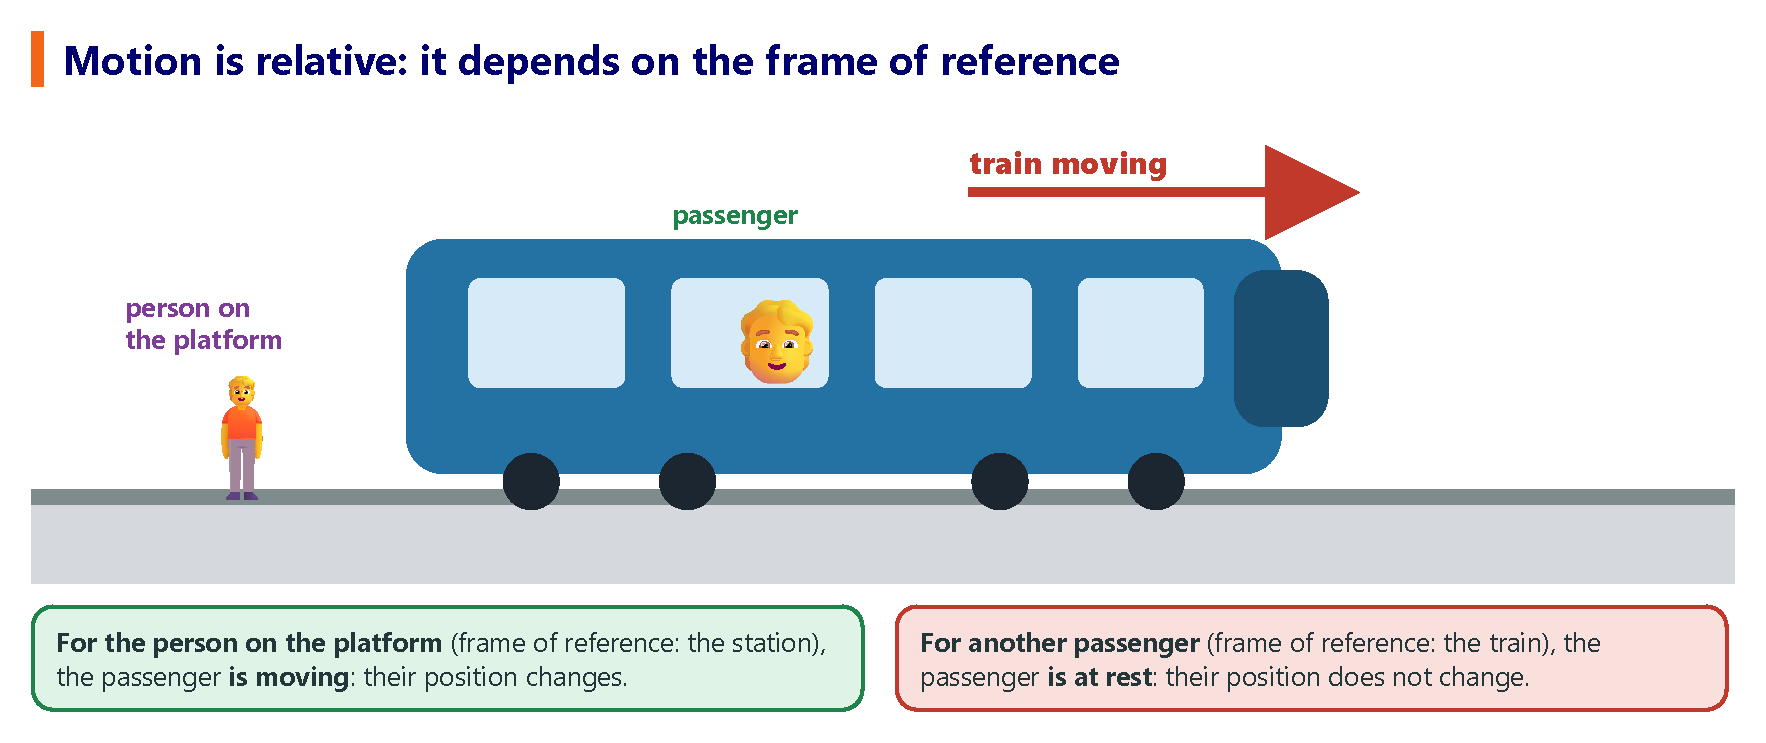
\includegraphics[width=\textwidth]{FigurasSVG/Unit_7_Motion/pdf/reference_frame.pdf}
        \caption{Whether the passenger moves or not depends on the frame of reference.}
        \label{fig:u7_reference_frame}
    \end{figure}

    \item \negsubro{Trajectory}.
    \begin{definition}[Trajectory]
        The line that a moving object follows. It can be \textbf{rectilinear} (straight), \textbf{circular}, \textbf{parabolic}, or any other shape.
    \end{definition}

    \item \negsubro{Position}.
    \begin{definition}[Position]
        The place occupied by a moving object at a given moment, measured from the origin of the frame of reference. It is represented by the letter \(x\).
    \end{definition}
    The position \(x\) tells us \textbf{how far} the object is from the origin, so it is a quantity of \textbf{length}: in the SI it is measured in \textbf{metres} (\unit{\m}). We write \(x_i\) for the \textbf{initial} position and \(x_f\) for the \textbf{final} position.

    \item \negsubro{Distance travelled}.
    \begin{definition}[Distance travelled]
        The length of the trajectory (path) followed by the moving object.
    \end{definition}

    \item \negsubro{Displacement}.
    \begin{definition}[Displacement]
        The change in position of a moving object: its final position minus its initial position. It is the straight-line distance between the initial and the final position.
        \begin{equation*}
            \Delta x = x_f - x_i
        \end{equation*}
    \end{definition}
    \begin{itemize}
        \item The symbol \(\Delta\) (the Greek letter \textbf{delta}) means ``\textbf{change in}'': \(\Delta x\) is read ``delta x'' and means ``change in position''.
        \item \(x_f\) is the \textbf{final} position and \(x_i\) the \textbf{initial} position. Both are positions, so \(\Delta x\) is also a \textbf{length} and is measured in \textbf{metres}.
        \item If \(\Delta x\) is \textbf{positive}, the object has moved away from the origin (in the positive direction); if it is \textbf{negative}, it has moved in the opposite direction.
    \end{itemize}
    \begin{figure}[H]
        \centering
        % [FIGURA ORIGINAL] \includegraphics[width=\textwidth]{Unit_7/delta_x_t}
        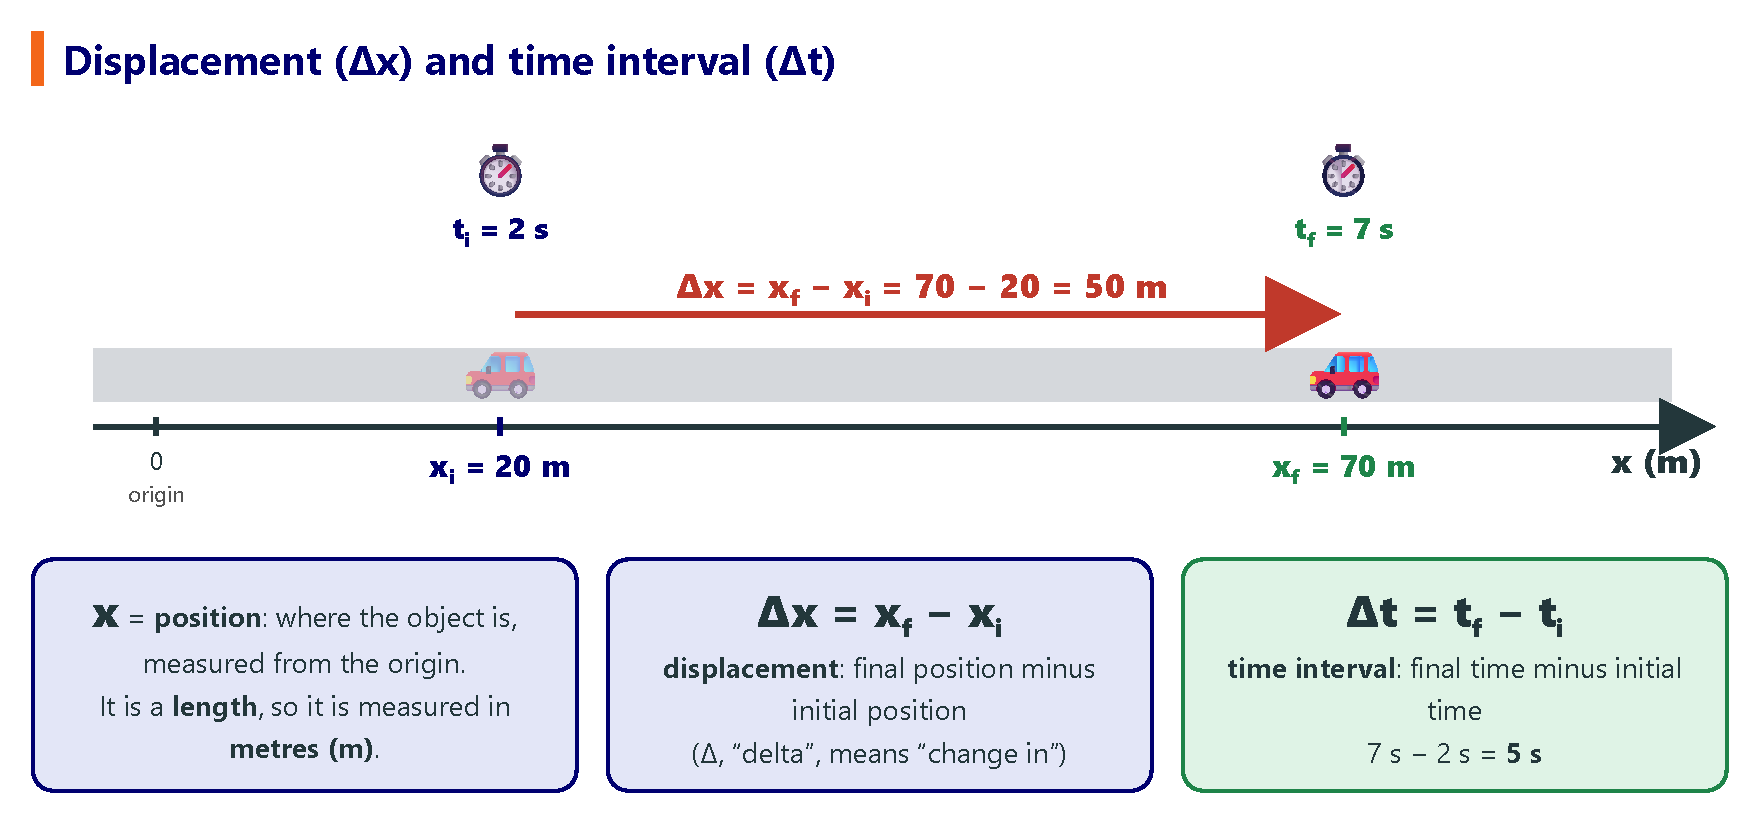
\includegraphics[width=\textwidth]{FigurasSVG/Unit_7_Motion/pdf/delta_x_t.pdf}
        \caption{The displacement is the final position minus the initial position; the time interval is the final time minus the initial time.}
        \label{fig:u7_delta_x_t}
    \end{figure}
    \begin{figure}[H]
        \centering
        % [FIGURA ORIGINAL] \includegraphics[width=\textwidth]{Unit_7/distance_displacement}
        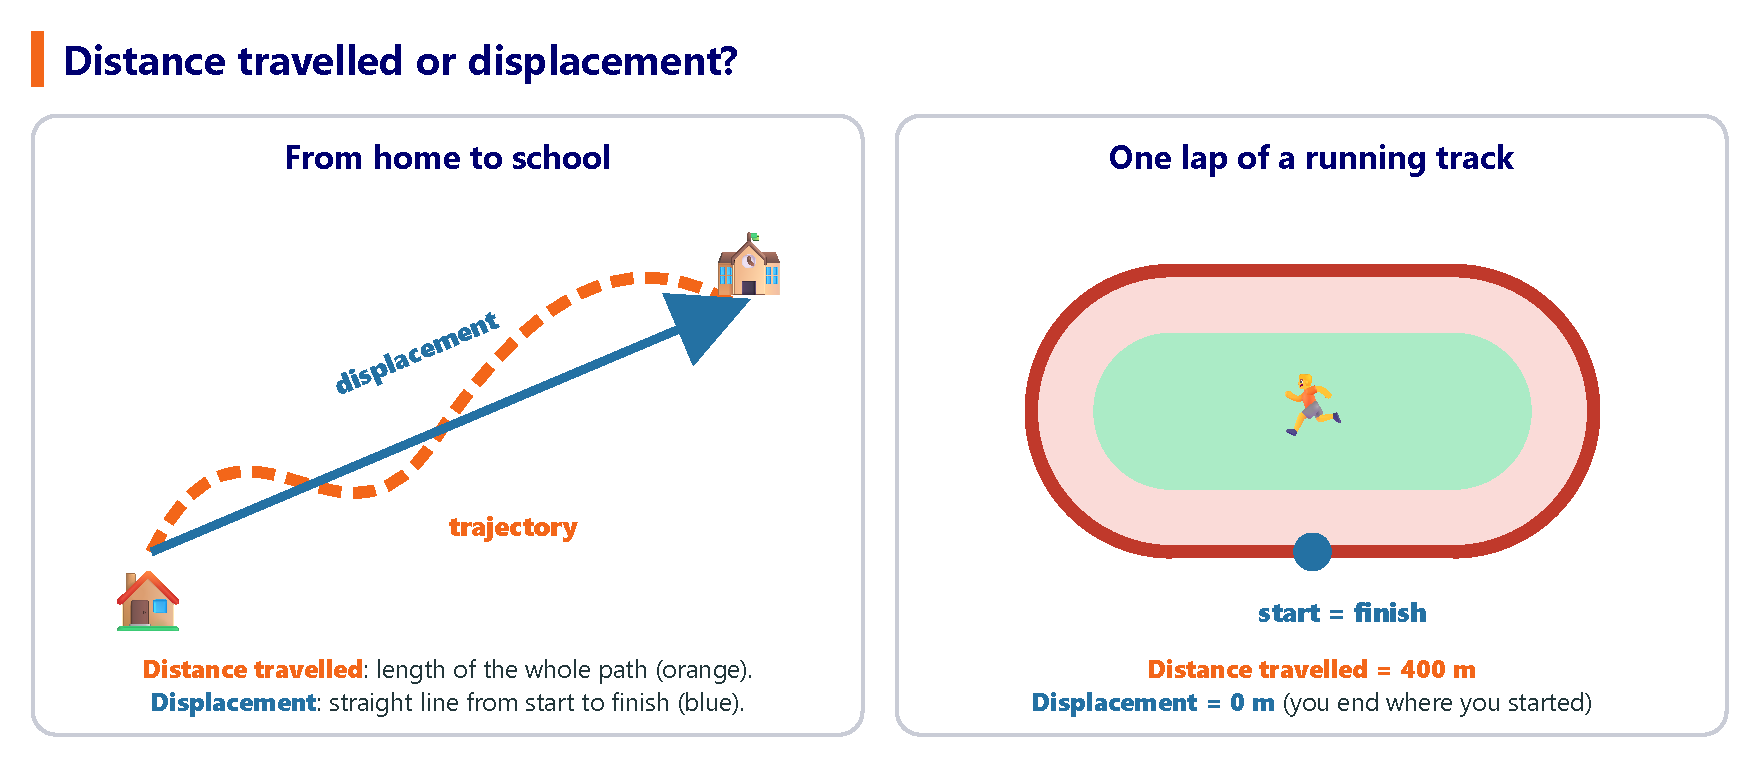
\includegraphics[width=\textwidth]{FigurasSVG/Unit_7_Motion/pdf/distance_displacement.pdf}
        \caption{Distance travelled (the whole path) and displacement (the straight line from start to finish).}
        \label{fig:u7_distance_displacement}
    \end{figure}
\end{enumerate}

\begin{example}
    \textbf{A car is at \(x_i = \qty{20}{\m}\) and, after a while, it is at \(x_f = \qty{70}{\m}\). Calculate its displacement.}
    \begin{equation*}
        \Delta x = x_f - x_i = \qty{70}{\m} - \qty{20}{\m} = \textcolor{red}{\qty{50}{\m}}
    \end{equation*}
\end{example}

\begin{exercise}
    A runner does one full lap of a \qty{400}{\m} circular track, starting and finishing at the same point.
    \begin{enumerate}[label=\letraminuscula]
        \item What distance has the runner travelled?
        \item What is the runner's displacement?
    \end{enumerate}
    \begin{solu}
        \begin{enumerate}[label=\alph*)]
            \item Distance travelled \(= \qty{400}{\m}\) (the length of the whole lap).
            \item Displacement \(= \qty{0}{\m}\), because the initial and final positions are the same point.
        \end{enumerate}
    \end{solu}
\end{exercise}

\begin{exercise}
    Two friends are sitting on parallel, stationary buses. Suddenly, one of the buses starts moving.
    \begin{enumerate}[label=\letraminuscula]
        \item Explain why, at first, it is difficult to tell which bus is moving.
        \item If you take the other bus as your frame of reference, can you tell which one is moving?
    \end{enumerate}
    \begin{solu}
        \begin{enumerate}[label=\alph*)]
            \item Motion is relative: from inside each bus, all you can perceive at first is the relative movement between the two buses, so it looks the same whichever one is actually moving.
            \item Yes: if you take the other bus as the fixed frame of reference, you can tell that \emph{your} bus is moving with respect to it as soon as the distance between the two buses changes.
        \end{enumerate}
    \end{solu}
\end{exercise}

\begin{exercise}
    A cyclist rides \qty{300}{\m} north along a straight road, then turns around and rides back \qty{120}{\m} south.
    \begin{enumerate}[label=\letraminuscula]
        \item Calculate the distance travelled.
        \item Calculate the displacement.
    \end{enumerate}
    \begin{solu}
        \begin{enumerate}[label=\alph*)]
            \item Distance travelled \(= \qty{300}{\m} + \qty{120}{\m} = \qty{420}{\m}\) (we add up every metre covered, regardless of direction).
            \item Displacement \(= \qty{300}{\m} - \qty{120}{\m} = \qty{180}{\m}\) north (the straight-line distance between the starting point and the final point).
        \end{enumerate}
    \end{solu}
\end{exercise}

\begin{exercise}
    A hiker walks \qty{2}{\km} east along a straight path, then turns around and walks \qty{5}{\km} west.
    \begin{enumerate}[label=\letraminuscula]
        \item Calculate the distance travelled.
        \item Calculate the displacement.
    \end{enumerate}
    \begin{solu}
        \begin{enumerate}[label=\alph*)]
            \item Distance travelled \(= \qty{2}{\km} + \qty{5}{\km} = \qty{7}{\km}\).
            \item Displacement \(= \qty{5}{\km} - \qty{2}{\km} = \qty{3}{\km}\) west (the straight-line distance from the start to the final point, in the direction of the larger leg).
        \end{enumerate}
    \end{solu}
\end{exercise}

%----------------------------------------------------------------------------------------

\section{Velocity}

\begin{definition}[Velocity]
    A quantity that measures how fast an object changes its position. It is represented by the letter \(v\), and it is the \textbf{displacement} divided by the \textbf{time interval}:
    \begin{equation*}
        v = \dfrac{\Delta x}{\Delta t} = \dfrac{x_f - x_i}{t_f - t_i}
    \end{equation*}
    In the SI, velocity is measured in \unit{\mps}.
\end{definition}

\begin{itemize}
    \item \(\Delta x = x_f - x_i\) is the \textbf{displacement} (final position minus initial position), in metres.
    \item \(\Delta t = t_f - t_i\) is the \textbf{time interval}: the \textbf{final} time \(t_f\) minus the \textbf{initial} time \(t_i\), in seconds.
\end{itemize}

\begin{impt}
    \negsubro{When nothing else is said}: if the exercise does not give the initial position or the initial time, we take
    \begin{equation*}
        x_i = \qty{0}{\m} \qquad\text{and}\qquad t_i = \qty{0}{\s}
    \end{equation*}
    Then \(\Delta x = x_f - 0 = x_f\) and \(\Delta t = t_f - 0 = t_f\). We simply write \(x_f\) as \(x\) and \(t_f\) as \(t\), and the formula of velocity becomes:
    \begin{equation*}
        v = \dfrac{x}{t}
    \end{equation*}
\end{impt}

\begin{example}
    \textbf{A car is at \(x_i = \qty{20}{\m}\) when the stopwatch reads \(t_i = \qty{2}{\s}\), and at \(x_f = \qty{70}{\m}\) when it reads \(t_f = \qty{7}{\s}\). Calculate its velocity.}
    \begin{equation*}
        v = \dfrac{x_f - x_i}{t_f - t_i} = \dfrac{\qty{70}{\m} - \qty{20}{\m}}{\qty{7}{\s} - \qty{2}{\s}} = \dfrac{\qty{50}{\m}}{\qty{5}{\s}} = \textcolor{red}{\qty{10}{\mps}}
    \end{equation*}
\end{example}

\begin{example}
    \textbf{A runner covers \qty{100}{\m} in \qty{12.5}{\s}. Calculate her velocity.} Nothing is said about the start, so \(x_i = \qty{0}{\m}\) and \(t_i = \qty{0}{\s}\):
    \begin{equation*}
        v = \dfrac{x}{t} = \dfrac{\qty{100}{\m}}{\qty{12.5}{\s}} = \textcolor{red}{\qty{8}{\mps}}
    \end{equation*}
\end{example}

In everyday language we often say \textbf{speed} for how fast something moves. Other common units are \unit{\kmph}, m/min, miles per hour or knots. To compare speeds given in different units, we must first convert them to the \textbf{same} unit, using conversion factors.

\begin{figure}[H]
    \centering
    % [FIGURA ORIGINAL] \includegraphics[width=\textwidth]{Unit_7/speeds}
    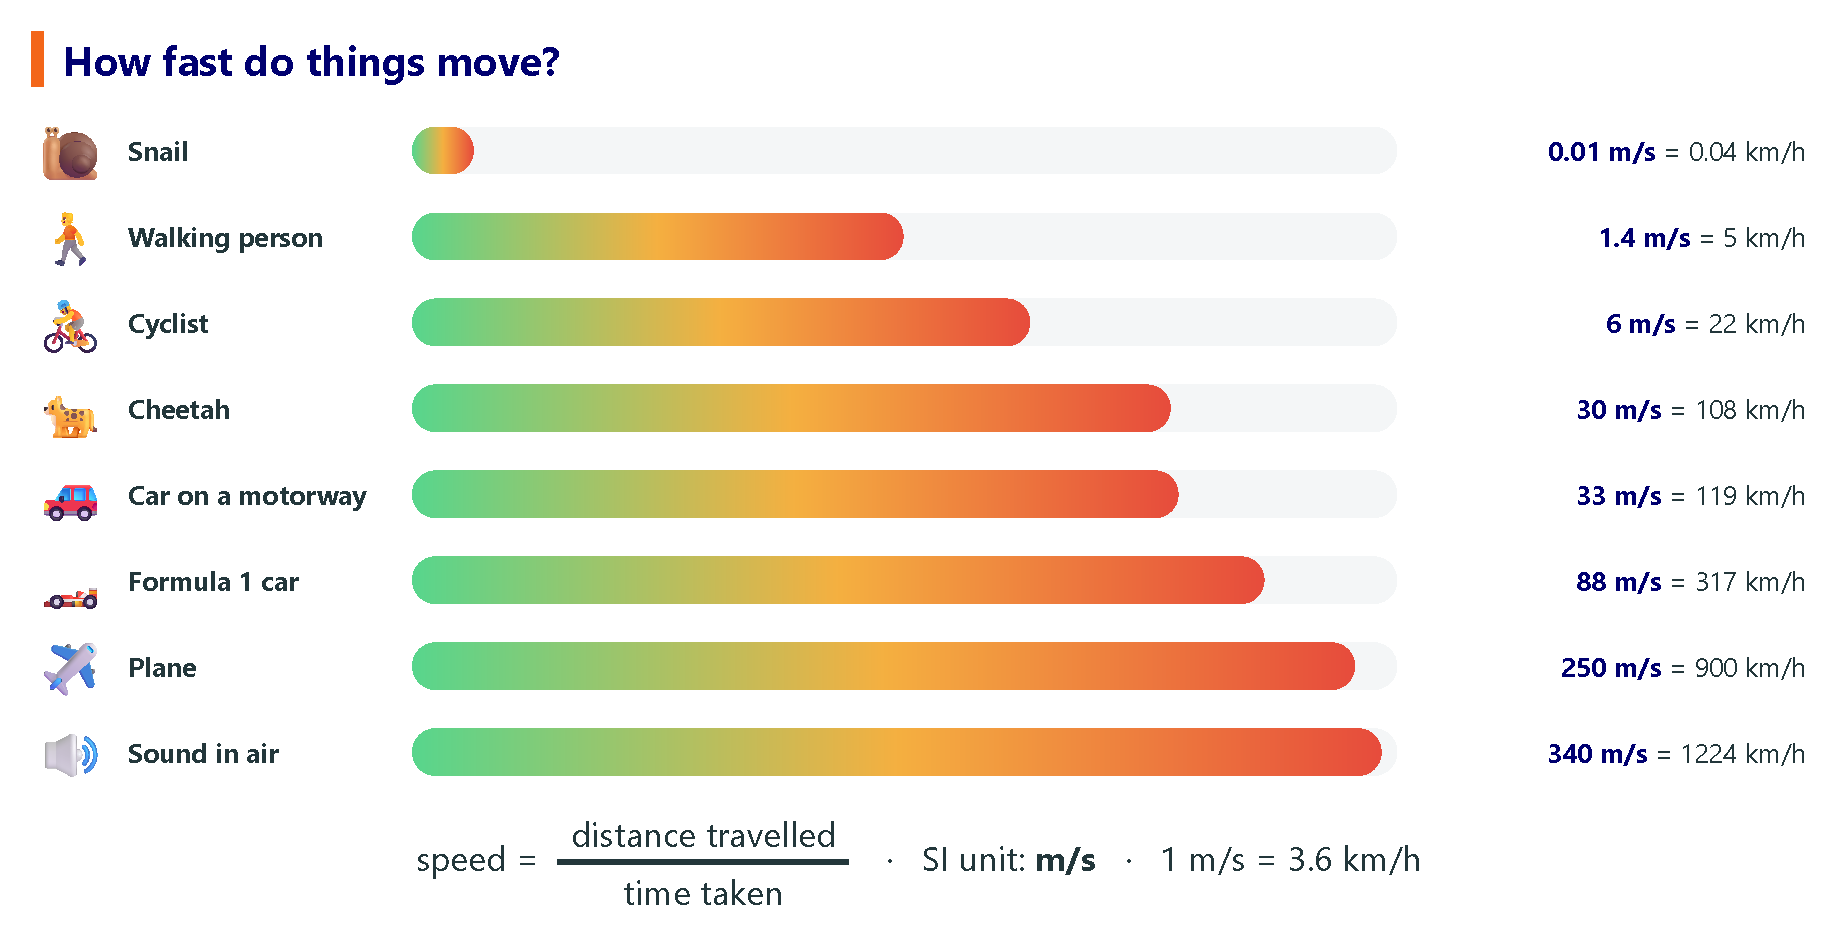
\includegraphics[width=\textwidth]{FigurasSVG/Unit_7_Motion/pdf/speeds.pdf}
    \caption{Speeds of some animals, vehicles and sound, in m/s and km/h.}
    \label{fig:u7_speeds}
\end{figure}

\begin{didyouknow}
    Even when you are sitting still in class, you are travelling at about \qty{107000}{\kmph}! That is the speed of the Earth in its orbit around the Sun. Motion really is relative.
\end{didyouknow}

\begin{example}
    \textbf{A car is travelling at \qty{90}{\kmph} and a motorbike at \qty{30}{\mps}. Which one is moving faster?}
    \begin{equation*}
        90 \dfrac{\text{km}}{\text{h}} \cdot \dfrac{\qty{1000}{\m}}{\qty{1}{\km}} \cdot \dfrac{\qty{1}{\hour}}{\qty{3600}{\s}} = \qty{25}{\mps}
    \end{equation*}
    Since \qty{30}{\mps} \(>\) \qty{25}{\mps}, \textbf{the motorbike is moving faster}.
\end{example}

\subsection{Average velocity and instantaneous velocity}

\begin{itemize}
    \item \negsubro{Average velocity}: the total distance travelled divided by the total time taken for a whole journey.
    \item \negsubro{Instantaneous velocity}: the velocity of a moving object at one specific moment, read on a speedometer.
\end{itemize}

\begin{impt}
    A moving object's velocity is usually \textbf{not} constant throughout a journey, so its average velocity is generally different from its instantaneous velocity at any given moment. They can only be the same if the object moves at a constant velocity for the whole journey.
\end{impt}

\begin{example}
    \textbf{A bus covers \qty{1500}{\m} in \qty{150}{\s}. Calculate its average velocity.}
    \begin{equation*}
        v_{\text{average}} = \dfrac{x}{t} = \dfrac{\qty{1500}{\m}}{\qty{150}{\s}} = \qty{10}{\mps} = \qty{36}{\kmph}
    \end{equation*}
\end{example}

\begin{exercise}
    Which animal is travelling faster: a centipede at \qty{40}{\cm\per\s}, or a tortoise at \qty{16.8}{\m\per\minute}?
    \begin{solu}
        Convert both to the same unit, \unit{\cm\per\s}: \\
        Tortoise: \(16.8 \dfrac{\text{m}}{\text{min}} \cdot \dfrac{\qty{100}{\cm}}{\qty{1}{\m}} \cdot \dfrac{\qty{1}{\minute}}{\qty{60}{\s}} = \qty{28}{\cm\per\s}\). \\
        Since \qty{40}{\cm\per\s} \(>\) \qty{28}{\cm\per\s}, \textbf{the centipede is faster}.
    \end{solu}
\end{exercise}

\begin{exercise}
    A commercial plane's cruising speed is \qty{900}{\kmph}. The maximum speed reached in a Formula 1 race was \qty{88}{\mps}. Which is higher?
    \begin{solu}
        Convert the plane's speed to \unit{\mps}: \(900 \dfrac{\text{km}}{\text{h}} \cdot \dfrac{\qty{1000}{\m}}{\qty{1}{\km}} \cdot \dfrac{\qty{1}{\hour}}{\qty{3600}{\s}} = \qty{250}{\mps}\). \\
        Since \qty{250}{\mps} \(>\) \qty{88}{\mps}, \textbf{the plane's cruising speed is higher}.
    \end{solu}
\end{exercise}

\begin{exercise}
    A lorry driver covers the \qty{300}{\km} between two cities. For the first \qty{200}{\km} she drives at an average speed of \qty{100}{\kmph}, and for the remaining \qty{100}{\km}, due to traffic, her average speed drops to \qty{50}{\kmph}.
    \begin{enumerate}[label=\letraminuscula]
        \item Calculate the time taken for each part of the journey.
        \item Calculate the average speed for the whole journey. Is it the mean of \qty{100}{\kmph} and \qty{50}{\kmph}? Explain why, or why not.
    \end{enumerate}
    \begin{solu}
        \begin{enumerate}[label=\alph*)]
            \item \(t_1 = \dfrac{\qty{200}{\km}}{\qty{100}{\kmph}} = \qty{2}{\hour}\); \quad \(t_2 = \dfrac{\qty{100}{\km}}{\qty{50}{\kmph}} = \qty{2}{\hour}\).
            \item Total distance \(= \qty{300}{\km}\); total time \(= 2 + 2 = \qty{4}{\hour}\). \\
            \(v_{\text{average}} = \dfrac{300}{4} = \qty{75}{\kmph}\). \\
            This \textbf{does coincide}, in this particular case, with the arithmetic mean of \qty{100}{\kmph} and \qty{50}{\kmph}, because the two parts happen to take the \textbf{same amount of time} (\qty{2}{\hour} each). In general, average speed is \textbf{not} the mean of the partial speeds: it must always be calculated as total distance divided by total time.
        \end{enumerate}
    \end{solu}
\end{exercise}

\begin{exercise}
    A train covers the first \qty{60}{\km} of a journey at a constant \qty{120}{\kmph}. It then stops at a station for \qty{15}{\minute}, and finally covers the last \qty{40}{\km} at a constant \qty{80}{\kmph}.
    \begin{enumerate}[label=\letraminuscula]
        \item Calculate the time taken for each of the three stages.
        \item Calculate the average speed for the whole journey (including the stop).
    \end{enumerate}
    \begin{solu}
        \begin{enumerate}[label=\alph*)]
            \item \(t_1 = \dfrac{\qty{60}{\km}}{\qty{120}{\kmph}} = \qty{0.5}{\hour}\); \quad \(t_2 = \qty{15}{\minute} = \qty{0.25}{\hour}\); \quad \(t_3 = \dfrac{\qty{40}{\km}}{\qty{80}{\kmph}} = \qty{0.5}{\hour}\).
            \item Total distance \(= 60 + 40 = \qty{100}{\km}\); total time \(= 0.5 + 0.25 + 0.5 = \qty{1.25}{\hour}\). \\
            \(v_{\text{average}} = \dfrac{100}{1.25} = \qty{80}{\kmph}\).
        \end{enumerate}
    \end{solu}
\end{exercise}

%----------------------------------------------------------------------------------------

\section{Uniform rectilinear motion (URM)}

\begin{definition}[Uniform rectilinear motion (URM)]
    The motion of an object that follows a straight trajectory at a \textbf{constant} velocity: it travels the same distance in each equal period of time.
\end{definition}

\subsection{Calculating position and time in URM}

In a URM the velocity is constant, so we can use \(v = \dfrac{x}{t}\) (taking \(x_i = \qty{0}{\m}\) and \(t_i = \qty{0}{\s}\)) to calculate not only the velocity, but also the \textbf{position} \(x\) or the \textbf{time} \(t\). First we must \textbf{isolate} the quantity we want, exactly as we did with the density in Unit 1: an equation is like a balanced scale, and we do the \textbf{same operation on both sides}.

\begin{figure}[H]
    \centering
    % [FIGURA ORIGINAL] \includegraphics[width=\textwidth]{Unit_7/velocity_isolate}
    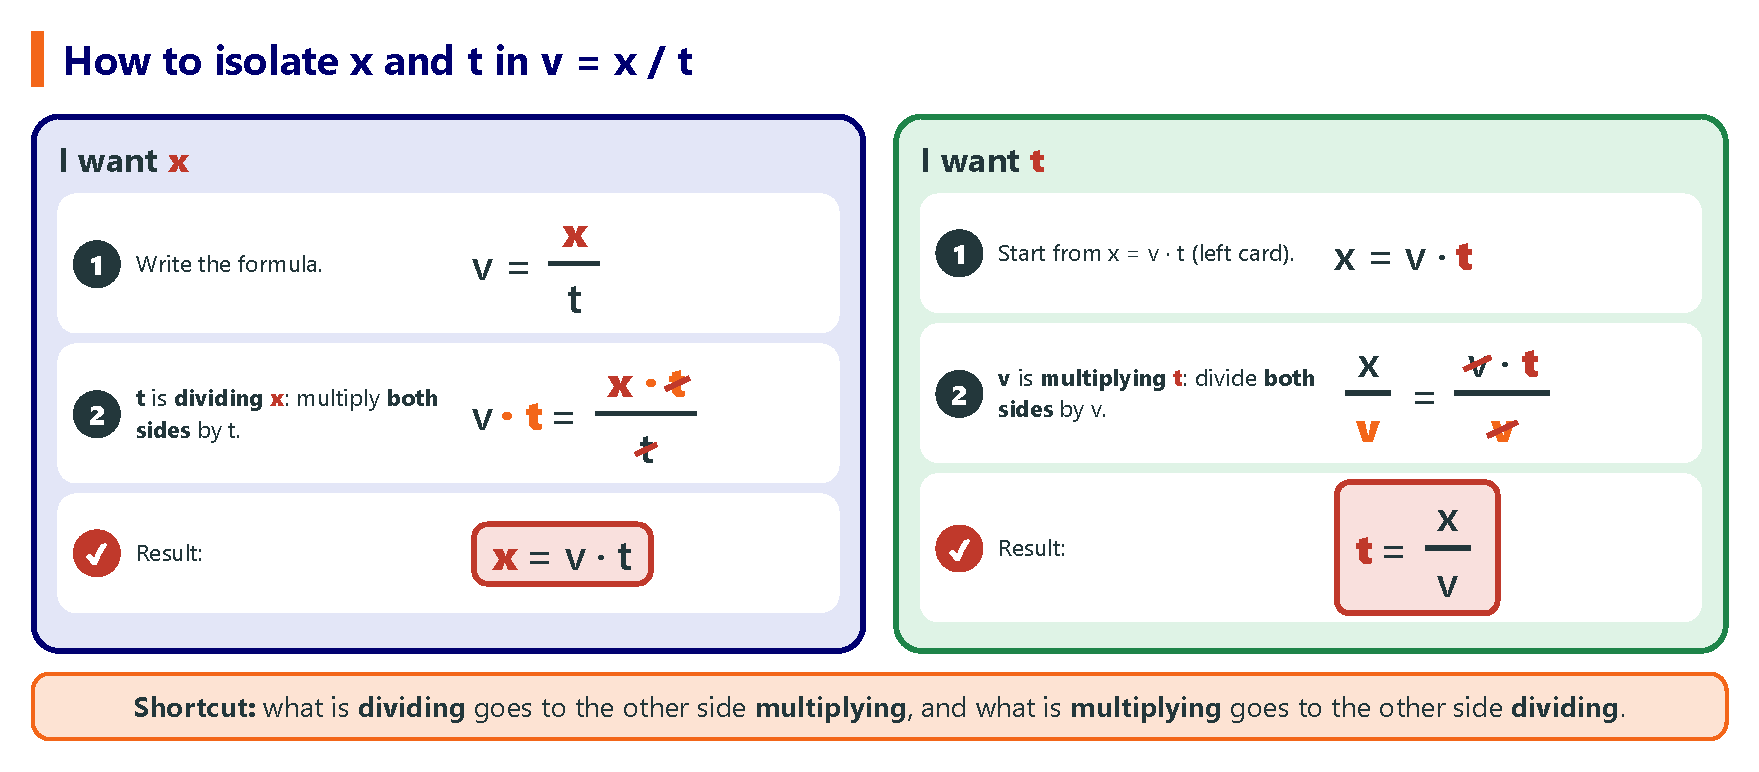
\includegraphics[width=\textwidth]{FigurasSVG/Unit_7_Motion/pdf/velocity_isolate.pdf}
    \caption{Isolating the position \(x\) and the time \(t\) in \(v = x/t\), step by step.}
    \label{fig:u7_velocity_isolate}
\end{figure}

\negsubro{Isolating the position \(x\)}:
\begin{enumerate}[label=\numberballmDarkTeal]
    \item We write the formula: \(v = \dfrac{x}{t}\).
    \item \(t\) is \textbf{dividing} \(x\), so we \textbf{multiply both sides} by \(t\): \(\;v \cdot t = \dfrac{x \cdot \cancelred{t}}{\cancelred{t}}\).
    \item \(t/t = 1\), so it cancels. We turn the equation round: \(\textcolor{red}{x = v \cdot t}\).
\end{enumerate}

\negsubro{Isolating the time \(t\)}:
\begin{enumerate}[label=\numberballmDarkTeal]
    \item We start from \(x = v \cdot t\) (the result above).
    \item \(v\) is \textbf{multiplying} \(t\), so we \textbf{divide both sides} by \(v\): \(\;\dfrac{x}{v} = \dfrac{\cancelred{v} \cdot t}{\cancelred{v}}\).
    \item \(v/v = 1\), so it cancels. We turn the equation round: \(\textcolor{red}{t = \dfrac{x}{v}}\).
\end{enumerate}

\begin{impt}
    The three versions of the same formula (with \(x_i = \qty{0}{\m}\) and \(t_i = \qty{0}{\s}\)):
    \begin{equation*}
        v = \dfrac{x}{t} \qquad\qquad x = v \cdot t \qquad\qquad t = \dfrac{x}{v}
    \end{equation*}
    \textbf{Shortcut}: what is \textbf{dividing} on one side goes to the other side \textbf{multiplying}, and what is \textbf{multiplying} goes to the other side \textbf{dividing}.
\end{impt}

\begin{example}
    \textbf{Calculating a position. A cyclist rides at a constant \qty{6}{\mps} for \qty{50}{\s}. Where is she at the end, if she started at the origin?}
    \begin{enumerate}[label=\numberballmDarkTeal]
        \item Data: \(v = \qty{6}{\mps}\), \(t = \qty{50}{\s}\), \(x_i = \qty{0}{\m}\). Unknown: \(\underline{x}\).
        \item Formula: \(v = \dfrac{x}{t}\). \(t\) is dividing, so it goes to the other side multiplying: \(x = v \cdot t\).
        \item \(x = \qty{6}{\mps} \cdot \qty{50}{\s} = \textcolor{red}{\qty{300}{\m}}\).
    \end{enumerate}
\end{example}

\begin{example}
    \textbf{Calculating a time. How long does a walker moving at a constant \qty{1.5}{\mps} take to walk \qty{1200}{\m}?}
    \begin{enumerate}[label=\numberballmDarkTeal]
        \item Data: \(v = \qty{1.5}{\mps}\), \(x = \qty{1200}{\m}\). Unknown: \(\underline{t}\).
        \item Formula: \(x = v \cdot t\). \(v\) is multiplying, so it goes to the other side dividing: \(t = \dfrac{x}{v}\).
        \item \(t = \dfrac{\qty{1200}{\m}}{\qty{1.5}{\mps}} = \textcolor{red}{\qty{800}{\s}}\) (about \qty{13.3}{\minute}).
    \end{enumerate}
\end{example}

\begin{exercise}
    Isolate the unknown and calculate (all the objects start at the origin and move in URM):
    \begin{enumerate}[label=\letraminuscula]
        \item The position of a car that travels at \qty{25}{\mps} for \qty{40}{\s}.
        \item The time a snail moving at \qty{0.002}{\mps} needs to travel \qty{1}{\m}.
        \item The time sound needs to travel \qty{1700}{\m} (\(v = \qty{340}{\mps}\)).
        \item The position of a train moving at \qty{30}{\mps} after \qty{2}{\minute} (change the time to seconds first).
    \end{enumerate}
    \begin{solu}
        \begin{enumerate}[label=\alph*)]
            \item \(x = v \cdot t = \qty{25}{\mps} \cdot \qty{40}{\s} = \qty{1000}{\m}\).
            \item \(t = \dfrac{x}{v} = \dfrac{\qty{1}{\m}}{\qty{0.002}{\mps}} = \qty{500}{\s}\).
            \item \(t = \dfrac{x}{v} = \dfrac{\qty{1700}{\m}}{\qty{340}{\mps}} = \qty{5}{\s}\).
            \item \(t = \qty{2}{\minute} = \qty{120}{\s}\); \(x = v \cdot t = \qty{30}{\mps} \cdot \qty{120}{\s} = \qty{3600}{\m}\).
        \end{enumerate}
    \end{solu}
\end{exercise}

\subsection{Position-time graphs in URM}

\begin{figure}[H]
    \centering
    % [FIGURA ORIGINAL] \includegraphics[width=\textwidth]{Unit_7/urm_graphs}
    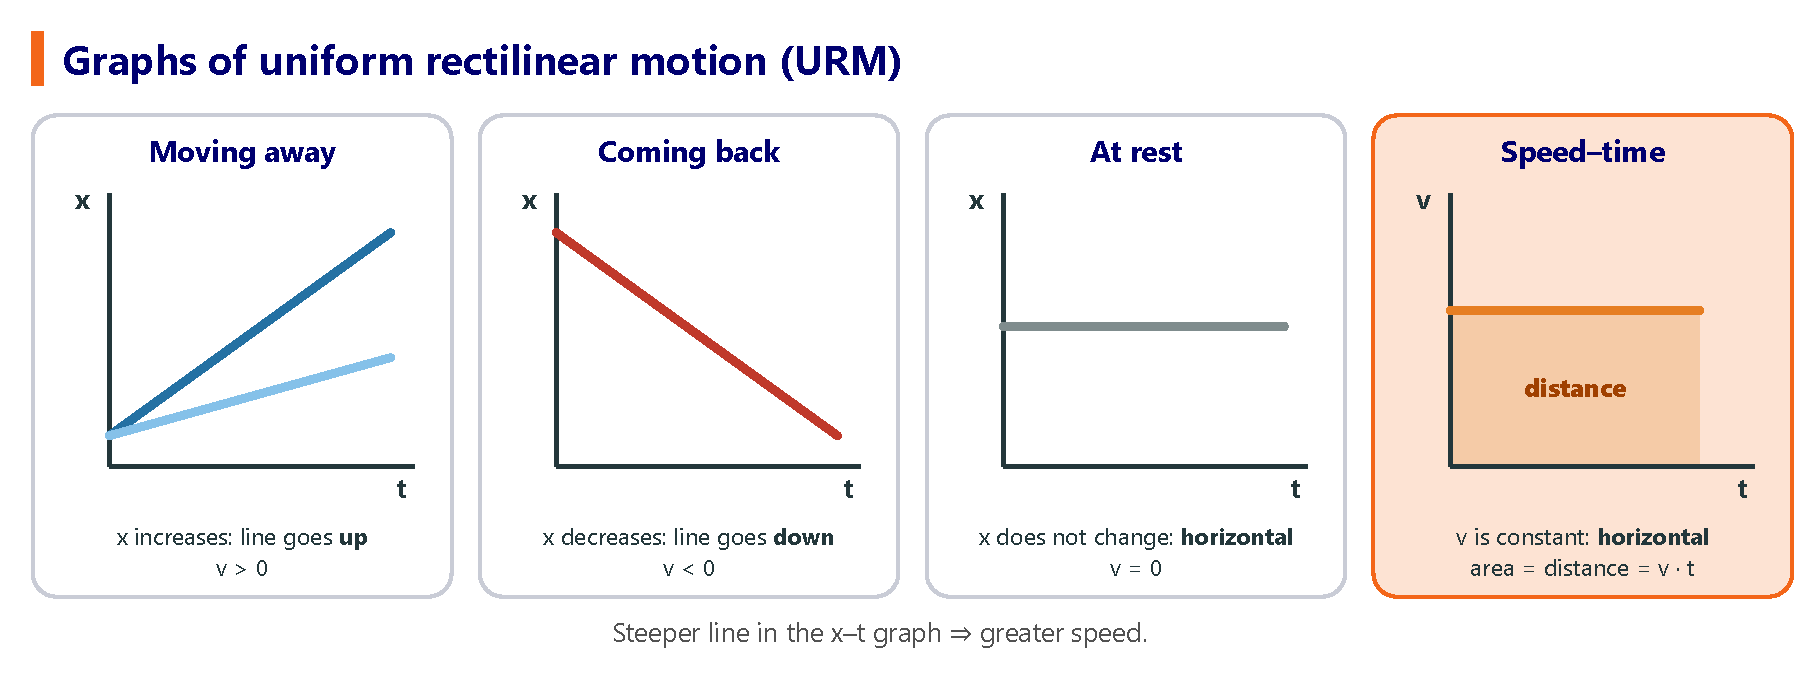
\includegraphics[width=\textwidth]{FigurasSVG/Unit_7_Motion/pdf/urm_graphs.pdf}
    \caption{Position-time and speed-time graphs of a URM.}
    \label{fig:u7_urm_graphs}
\end{figure}

\begin{itemize}
    \item If the position \textbf{increases} with time, the line goes up, and the object is moving away from the origin.
    \item If the position \textbf{decreases} with time, the line goes down, and the object is moving towards the origin (or past it, into negative positions).
    \item The graph of a URM is always a \textbf{straight line}. The more inclined the line, the greater the speed.
    \item If the line passes through the point \((0,0)\), the object was at the origin when we started studying its motion; if not, the object was already at another position.
\end{itemize}

\begin{impt}
    \negsubro{Reading two URM lines on the same graph}: when two position-time lines are drawn on the same axes, the point where they \textbf{cross} represents the moment and the position at which the two objects meet (they are, at that instant, at the same place).
\end{impt}

\begin{figure}[H]
    \centering
    % [FIGURA ORIGINAL] \includegraphics[width=0.95\textwidth]{Unit_7/meeting}
    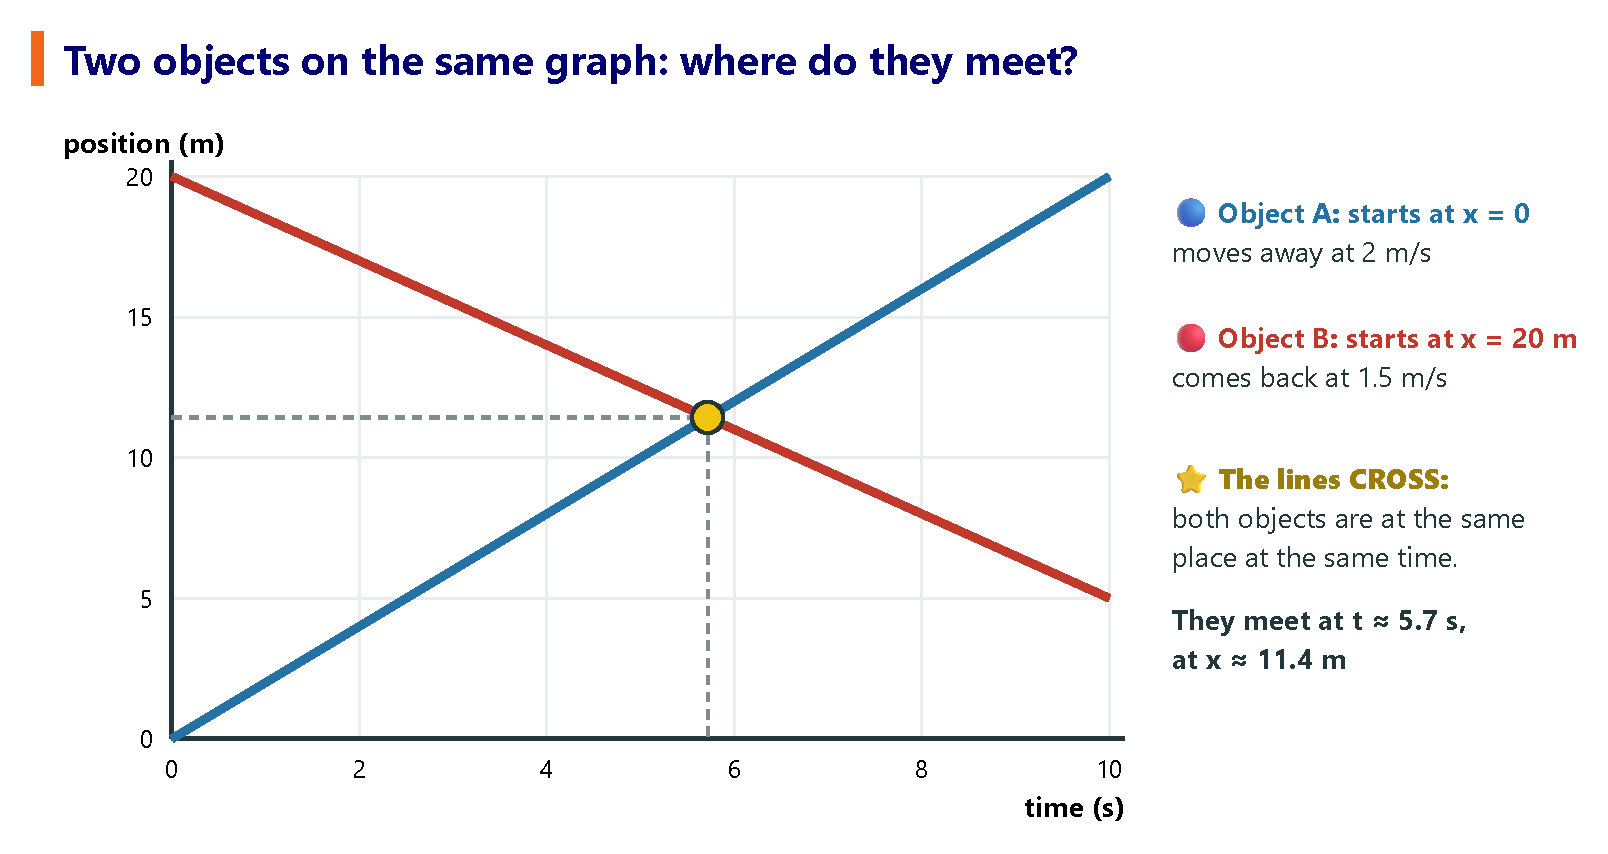
\includegraphics[width=0.95\textwidth]{FigurasSVG/Unit_7_Motion/pdf/meeting.pdf}
    \caption{When two position-time lines cross, the two objects are at the same place at the same time.}
    \label{fig:u7_meeting}
\end{figure}

\begin{example}
    \textbf{Two positions are recorded for a walker every second: at \(t=\qty{2}{\s}\), \(x=\qty{3}{\m}\); at \(t=\qty{6}{\s}\), \(x=\qty{11}{\m}\). Is the position-time graph increasing or decreasing? What does this tell us about the walker's direction?}

    Since \(x\) increases from \(\qty{3}{\m}\) to \(\qty{11}{\m}\) as \(t\) increases, the line on the position-time graph goes \textbf{up}: the walker is moving \textbf{away} from the origin. The speed can also be found from these two points: \(v = \dfrac{11-3}{6-2} = \qty{2}{\mps}\).
\end{example}

\begin{exercise}
    A position-time graph shows a straight horizontal line at \(x = \qty{12}{\m}\), from \(t=0\) to \(t=\qty{10}{\s}\).
    \begin{enumerate}[label=\letraminuscula]
        \item What is the object's speed?
        \item Is the object moving with respect to the chosen frame of reference?
    \end{enumerate}
    \begin{solu}
        \begin{enumerate}[label=\alph*)]
            \item Since the position does not change, \(v = \qty{0}{\mps}\).
            \item No: a horizontal line on a position-time graph means the object stays at the same position, so it is \textbf{at rest} with respect to this frame of reference.
        \end{enumerate}
    \end{solu}
\end{exercise}

\begin{exercise}
    The position-time graph of an object in URM is a straight line that passes through the origin \((0,0)\) and through the point \((t,x) = (\qty{5}{\s}, \qty{15}{\m})\).
    \begin{enumerate}[label=\letraminuscula]
        \item Was the object at the origin at \(t=0\)?
        \item Calculate its speed.
        \item Predict its position at \(t=\qty{8}{\s}\).
    \end{enumerate}
    \begin{solu}
        \begin{enumerate}[label=\alph*)]
            \item Yes: the line passes through \((0,0)\), so the object started at the origin.
            \item \(v = \dfrac{\qty{15}{\m} - 0}{\qty{5}{\s} - 0} = \qty{3}{\mps}\).
            \item \(x(8) = v \cdot t = \qty{3}{\mps} \cdot \qty{8}{\s} = \qty{24}{\m}\).
        \end{enumerate}
    \end{solu}
\end{exercise}

\begin{exercise}
    The position-time graph of a URM is shown below.
    \begin{center}
        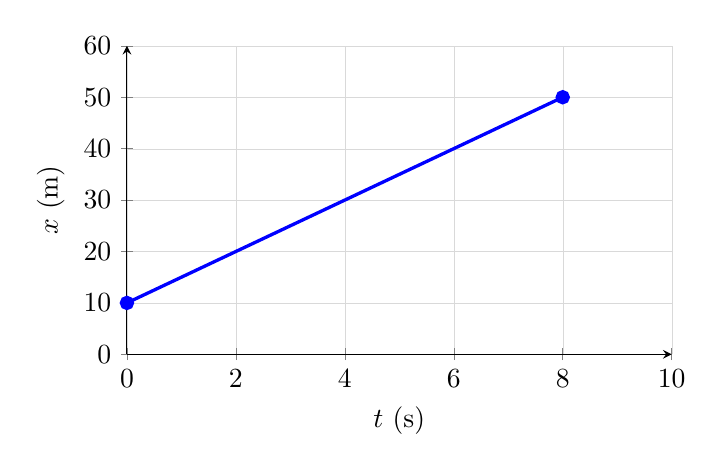
\begin{tikzpicture}
            \begin{axis}[width=8.5cm, height=5.5cm, grid=both, grid style={line width=.1pt, draw=gray!30},
                axis lines=left, xlabel={\(t\) (s)}, ylabel={\(x\) (m)}, xmin=0, xmax=10, ymin=0, ymax=60, xtick={0,2,...,10}, ytick={0,10,...,60}]
                \addplot[very thick, blue, mark=*] coordinates {(0,10) (8,50)};
            \end{axis}
        \end{tikzpicture}
    \end{center}
    \begin{enumerate}[label=\letraminuscula]
        \item What is the initial position \(x_i\) of the object?
        \item Calculate its velocity, using \(x_i\), \(x_f\), \(t_i\) and \(t_f\).
        \item Is the object moving away from the origin or towards it?
        \item Read on the graph the position at \(t = \qty{4}{\s}\), and check it with a calculation.
    \end{enumerate}
    \begin{solu}
        \begin{enumerate}[label=\alph*)]
            \item At \(t = \qty{0}{\s}\) the line starts at \(x_i = \qty{10}{\m}\): the object did not start at the origin.
            \item \(v = \dfrac{x_f - x_i}{t_f - t_i} = \dfrac{\qty{50}{\m} - \qty{10}{\m}}{\qty{8}{\s} - \qty{0}{\s}} = \qty{5}{\mps}\).
            \item The line goes up (\(v > 0\)): it is moving \textbf{away} from the origin.
            \item From the graph, \(x = \qty{30}{\m}\). Calculation: \(x = x_i + v \cdot t = \qty{10}{\m} + \qty{5}{\mps} \cdot \qty{4}{\s} = \qty{30}{\m}\).
        \end{enumerate}
    \end{solu}
\end{exercise}

\begin{exercise}
    The graph shows the position of a student walking along a straight corridor.
    \begin{center}
        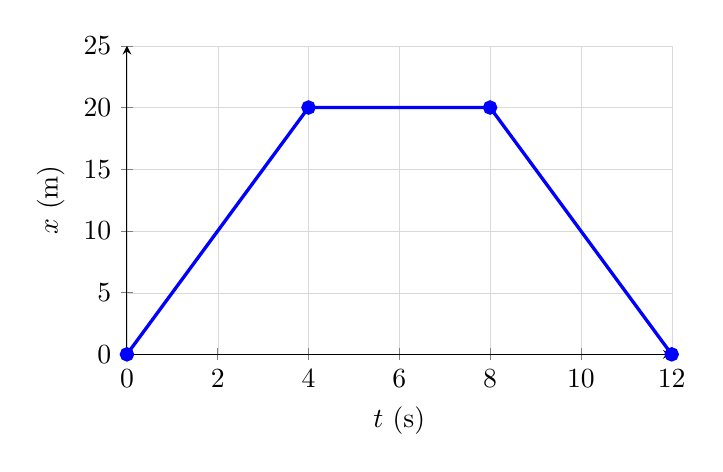
\begin{tikzpicture}
            \begin{axis}[width=8.5cm, height=5.5cm, grid=both, grid style={line width=.1pt, draw=gray!30},
                axis lines=left, xlabel={\(t\) (s)}, ylabel={\(x\) (m)}, xmin=0, xmax=12, ymin=0, ymax=25, xtick={0,2,...,12}, ytick={0,5,...,25}]
                \addplot[very thick, blue, mark=*] coordinates {(0,0) (4,20) (8,20) (12,0)};
            \end{axis}
        \end{tikzpicture}
    \end{center}
    \begin{enumerate}[label=\letraminuscula]
        \item Describe what the student does in each section: \(0\)--\(4\) s, \(4\)--\(8\) s and \(8\)--\(12\) s.
        \item Calculate the velocity in each section.
        \item Calculate the total distance travelled and the total displacement.
    \end{enumerate}
    \begin{solu}
        \begin{enumerate}[label=\alph*)]
            \item \(0\)--\(4\) s: moves away from the origin. \(4\)--\(8\) s: stays at \(x = \qty{20}{\m}\) (at rest). \(8\)--\(12\) s: comes back to the origin.
            \item \(v_1 = \dfrac{20 - 0}{4 - 0} = \qty{5}{\mps}\); \quad \(v_2 = \dfrac{20 - 20}{8 - 4} = \qty{0}{\mps}\); \quad \(v_3 = \dfrac{0 - 20}{12 - 8} = \qty{-5}{\mps}\).
            \item Distance travelled \(= \qty{20}{\m} + \qty{0}{\m} + \qty{20}{\m} = \qty{40}{\m}\). Displacement \(\Delta x = x_f - x_i = \qty{0}{\m} - \qty{0}{\m} = \qty{0}{\m}\) (he ends where he started).
        \end{enumerate}
    \end{solu}
\end{exercise}

\begin{exercise}
    The graph shows the positions of two cars, \(A\) and \(B\), moving along the same straight road.
    \begin{center}
        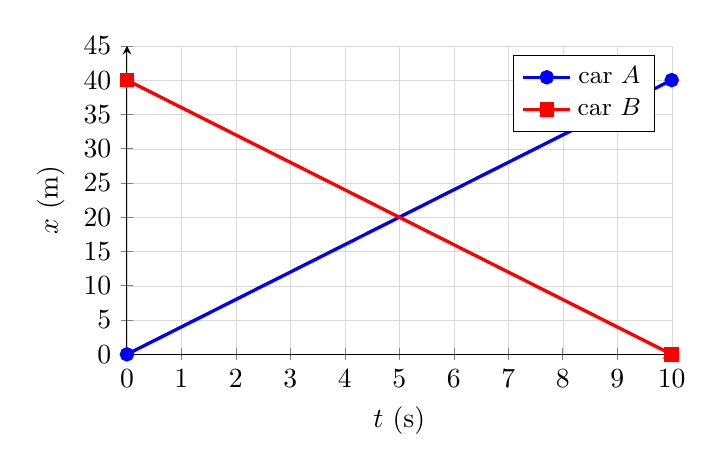
\begin{tikzpicture}
            \begin{axis}[width=8.5cm, height=5.5cm, grid=both, grid style={line width=.1pt, draw=gray!30},
                axis lines=left, xlabel={\(t\) (s)}, ylabel={\(x\) (m)}, xmin=0, xmax=10, ymin=0, ymax=45, xtick={0,1,...,10}, ytick={0,5,...,45}, legend pos=north east, legend style={font=\small}]
                \addplot[very thick, blue, mark=*] coordinates {(0,0) (10,40)};
                \addlegendentry{car \(A\)}
                \addplot[very thick, red, mark=square*] coordinates {(0,40) (10,0)};
                \addlegendentry{car \(B\)}
            \end{axis}
        \end{tikzpicture}
    \end{center}
    \begin{enumerate}[label=\letraminuscula]
        \item Calculate the velocity of each car. What does the sign of each velocity mean?
        \item At what time and in what position do the two cars meet?
    \end{enumerate}
    \begin{solu}
        \begin{enumerate}[label=\alph*)]
            \item \(v_A = \dfrac{40 - 0}{10 - 0} = \qty{4}{\mps}\) (positive: it moves away from the origin). \(v_B = \dfrac{0 - 40}{10 - 0} = \qty{-4}{\mps}\) (negative: it moves towards the origin).
            \item The lines cross at \(t = \qty{5}{\s}\) and \(x = \qty{20}{\m}\): the two cars meet there.
        \end{enumerate}
    \end{solu}
\end{exercise}

\begin{exercise}
    A toy car moves in URM. Its positions are recorded in this table:
    \begin{center}
        \begin{tabular}{lcccccc}
            \toprule
            \(t\) (s) & 0 & 1 & 2 & 3 & 4 & 5 \\
            \midrule
            \(x\) (m) & 0 & 3 & 6 & 9 & 12 & 15 \\
            \bottomrule
        \end{tabular}
    \end{center}
    \begin{enumerate}[label=\letraminuscula]
        \item Draw the position-time graph (\(t\) on the horizontal axis, \(x\) on the vertical axis).
        \item What shape does the graph have? Why?
        \item Calculate the velocity of the car.
    \end{enumerate}
    \begin{solu}
        \begin{enumerate}[label=\alph*)]
            \item The points \((0,0)\), \((1,3)\), \((2,6)\), \((3,9)\), \((4,12)\) and \((5,15)\) are joined with a straight line.
    \begin{center}
                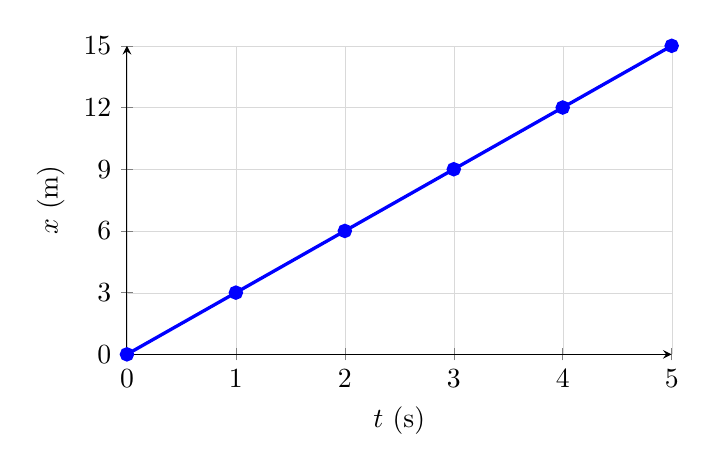
\begin{tikzpicture}
                    \begin{axis}[width=8.5cm, height=5.5cm, grid=both, grid style={line width=.1pt, draw=gray!30},
                        axis lines=left, xlabel={\(t\) (s)}, ylabel={\(x\) (m)}, xmin=0, xmax=5, ymin=0, ymax=15, xtick={0,1,...,5}, ytick={0,3,...,15}]
                        \addplot[very thick, blue, mark=*] coordinates {(0,0) (1,3) (2,6) (3,9) (4,12) (5,15)};
                    \end{axis}
                \end{tikzpicture}
            \end{center}
            \item A straight line going up through the origin, because the car covers the same distance (\qty{3}{\m}) every second: its velocity is constant.
            \item \(v = \dfrac{x_f - x_i}{t_f - t_i} = \dfrac{\qty{15}{\m} - \qty{0}{\m}}{\qty{5}{\s} - \qty{0}{\s}} = \qty{3}{\mps}\).
        \end{enumerate}
    \end{solu}
\end{exercise}

\subsection{Velocity in URM from a table or a graph}

To calculate the velocity of a URM, take any two points \(A\) and \(B\) from a table or graph. Point \(A\) is the \textbf{initial} one and point \(B\) the \textbf{final} one:
\begin{equation*}
    x_A = x_i \qquad t_A = t_i \qquad\qquad x_B = x_f \qquad t_B = t_f
\end{equation*}
So the formula is exactly the same formula of velocity that we already know:
\begin{equation*}
    v = \dfrac{x_B - x_A}{t_B - t_A} = \dfrac{x_f - x_i}{t_f - t_i} = \dfrac{\Delta x}{\Delta t}
\end{equation*}

\begin{example}
    \textbf{A point \(A\) is at \(x = \qty{10}{\m}\) when \(t = \qty{4}{\s}\); a point \(B\) is at \(x = \qty{30}{\m}\) when \(t = \qty{12}{\s}\). Find the velocity.} \\
    Point \(A\) is the initial one: \(x_i = \qty{10}{\m}\), \(t_i = \qty{4}{\s}\). Point \(B\) is the final one: \(x_f = \qty{30}{\m}\), \(t_f = \qty{12}{\s}\).
    \begin{equation*}
        v = \dfrac{\qty{30}{\m} - \qty{10}{\m}}{\qty{12}{\s} - \qty{4}{\s}} = \qty{2.5}{\mps}
    \end{equation*}
    A \textbf{positive} speed means the object is moving away from the origin.
\end{example}

\begin{impt}
    If, instead, the position \textbf{decreases} between the two points, the speed comes out \textbf{negative}. This means the object is moving towards the origin (or beyond it).
\end{impt}

\begin{exercise}
    A point \(A\) is at \(x = \qty{50}{\m}\) when \(t = \qty{5}{\s}\); a point \(B\) is at \(x = \qty{20}{\m}\) when \(t = \qty{15}{\s}\).
    \begin{enumerate}[label=\letraminuscula]
        \item Calculate the speed.
        \item What does the sign of the speed tell you about the direction of motion?
    \end{enumerate}
    \begin{solu}
        \begin{enumerate}[label=\alph*)]
            \item \(v = \dfrac{\qty{20}{\m} - \qty{50}{\m}}{\qty{15}{\s} - \qty{5}{\s}} = \qty{-3}{\mps}\).
            \item The speed is \textbf{negative}, so the object is moving towards the origin (its position decreases with time).
        \end{enumerate}
    \end{solu}
\end{exercise}

\begin{exercise}
    The table shows the position of a toy train every \qty{3}{\s}:
    \begin{center}
        \begin{tabular}{lcccc}
            \toprule
            Time (s) & 0 & 3 & 6 & 9 \\
            \midrule
            Position (m) & 2 & 14 & 26 & 38 \\
            \bottomrule
        \end{tabular}
    \end{center}
    \begin{enumerate}[label=\letraminuscula]
        \item Calculate the speed using the first two points in the table.
        \item Check, using another pair of points, that the motion is indeed a URM.
        \item Predict the train's position at \(t=\qty{12}{\s}\).
    \end{enumerate}
    \begin{solu}
        \begin{enumerate}[label=\alph*)]
            \item \(v = \dfrac{\qty{14}{\m} - \qty{2}{\m}}{\qty{3}{\s} - \qty{0}{\s}} = \qty{4}{\mps}\).
            \item Between \(t=6\) s and \(t=9\) s: \(v = \dfrac{38-26}{9-6} = \qty{4}{\mps}\), the same value, so the speed is constant: this confirms it is a URM.
            \item \(x(12) = x(0) + v \cdot t = \qty{2}{\m} + \qty{4}{\mps} \cdot \qty{12}{\s} = \qty{50}{\m}\).
        \end{enumerate}
    \end{solu}
\end{exercise}

\subsection{Velocity-time graphs in URM}

Since the velocity of a URM is constant, its velocity-time graph is always a \textbf{horizontal line}.

\begin{impt}
    \negsubro{Distance travelled from a speed-time graph}: the distance travelled equals the \textbf{area} between the speed-time line and the time axis. In a URM this area is a rectangle: \(\text{distance} = v \cdot t\), which is the same equation we already use to calculate the speed.
\end{impt}

\begin{example}
    \textbf{A cyclist moves at a constant \qty{4}{\mps} for \qty{15}{\s}. Find the distance travelled using the area under the speed-time graph.}

    The speed-time graph is a horizontal line at \(v = \qty{4}{\mps}\), between \(t=0\) and \(t=\qty{15}{\s}\). The area underneath is a rectangle:
    \begin{equation*}
        \text{distance} = v \cdot t = \qty{4}{\mps} \cdot \qty{15}{\s} = \qty{60}{\m}
    \end{equation*}
\end{example}

\begin{exercise}
    The table shows the position of a remote-controlled car every \qty{10}{\s}:
    \begin{center}
        \begin{tabular}{lcccc}
            \toprule
            Time (s) & 0 & 10 & 20 & 30 \\
            \midrule
            Position (m) & 10 & 30 & 30 & 0 \\
            \bottomrule
        \end{tabular}
    \end{center}
    \begin{enumerate}[label=\letraminuscula]
        \item Calculate the speed in each section of its journey.
        \item Calculate the average speed of the whole journey.
    \end{enumerate}
    \begin{solu}
        \begin{enumerate}[label=\alph*)]
            \item Section 1 (\(t=0\) to \(10\) s): \(v_1 = \dfrac{30-10}{10-0} = \qty{2}{\mps}\). \\
            Section 2 (\(t=10\) to \(20\) s): the position does not change, so \(v_2 = \qty{0}{\mps}\) (the car is at rest). \\
            Section 3 (\(t=20\) to \(30\) s): \(v_3 = \dfrac{0-30}{30-20} = \qty{-3}{\mps}\) (moving towards the origin).
            \item Total distance travelled \(= \qty{20}{\m} + \qty{0}{\m} + \qty{30}{\m} = \qty{50}{\m}\); total time \(= \qty{30}{\s}\). \\
            \(v_{\text{average}} = \dfrac{50}{30} \approx \qty{1.67}{\mps}\).
        \end{enumerate}
    \end{solu}
\end{exercise}

\begin{exercise}
    A cyclist passes the \qty{20}{\km} mark when the stopwatch is started, moving at a constant speed. She reaches the \qty{40}{\km} mark after \qty{25}{\minute}, stops to rest for \qty{20}{\minute}, and then travels the next \qty{20}{\km} in \qty{10}{\minute}, again at a constant speed.
    \begin{enumerate}[label=\letraminuscula]
        \item Calculate her speed in each of the three sections.
        \item Calculate her average speed for the whole journey.
    \end{enumerate}
    \begin{solu}
        \begin{enumerate}[label=\alph*)]
            \item Section 1: \(v_1 = \dfrac{40\qty{-20}{\km}}{25\qty{-0}{\minute}} = \qty{0.8}{\km\per\minute}\). \\
            Section 2 (resting): \(v_2 = \qty{0}{\km\per\minute}\). \\
            Section 3: \(v_3 = \dfrac{60\qty{-40}{\km}}{55\qty{-45}{\minute}} = \qty{2}{\km\per\minute}\).
            \item Total distance \(= \qty{40}{\km}\); total time \(= 25 + 20 + 10 = \qty{55}{\minute}\) (the rest is included). \\
            \(v_{\text{average}} = \dfrac{40}{55} \approx \qty{0.73}{\km\per\minute}\).
        \end{enumerate}
    \end{solu}
\end{exercise}

\begin{exercise}
    Two trains, \(A\) and \(B\), travel towards each other along the same straight track. Train \(A\) starts at position \(x=\qty{0}{\km}\) and moves at \(\qty{80}{\kmph}\). Train \(B\) starts, at the same instant, at position \(x=\qty{300}{\km}\) and moves at \(\qty{70}{\kmph}\) towards \(A\).
    \begin{enumerate}[label=\letraminuscula]
        \item Write the position of each train as a function of time, \(x_A(t)\) and \(x_B(t)\).
        \item Find the time and the position at which the two trains meet.
    \end{enumerate}
    \begin{solu}
        \begin{enumerate}[label=\alph*)]
            \item \(x_A(t) = 80 \cdot t\) (moving away from the origin). \\
            \(x_B(t) = 300 - 70 \cdot t\) (moving towards the origin).
            \item They meet when \(x_A(t) = x_B(t)\): \(80t = 300 - 70t \;\Rightarrow\; 150t = 300 \;\Rightarrow\; t = \qty{2}{\hour}\). \\
            Position: \(x_A(2) = 80 \cdot 2 = \qty{160}{\km}\) (checking: \(x_B(2) = 300 - 70\cdot 2 = \qty{160}{\km}\), the same). \\
            The trains meet after \qty{2}{\hour}, at \(x = \qty{160}{\km}\).
        \end{enumerate}
    \end{solu}
\end{exercise}

\begin{exercise}
    A scooter moves at a constant \qty{3}{\mps} for \qty{20}{\s}, then stops for \qty{10}{\s}, and finally moves at a constant \qty{6}{\mps} for \qty{5}{\s}.
    \begin{enumerate}[label=\letraminuscula]
        \item Describe the shape of the speed-time graph in each of the three stages.
        \item Calculate the distance travelled in each stage, using the area under the graph.
        \item Calculate the average speed for the whole journey.
    \end{enumerate}
    \begin{solu}
        \begin{enumerate}[label=\alph*)]
            \item Stage 1: horizontal line at \(v=\qty{3}{\mps}\). Stage 2: horizontal line at \(v=\qty{0}{\mps}\) (on the time axis). Stage 3: horizontal line at \(v=\qty{6}{\mps}\).
            \item Stage 1: \(d_1 = \qty{3}{\mps} \cdot \qty{20}{\s} = \qty{60}{\m}\). Stage 2: \(d_2 = \qty{0}{\m}\). Stage 3: \(d_3 = \qty{6}{\mps} \cdot \qty{5}{\s} = \qty{30}{\m}\).
            \item Total distance \(= 60 + 0 + 30 = \qty{90}{\m}\); total time \(= 20+10+5 = \qty{35}{\s}\). \\
            \(v_{\text{average}} = \dfrac{90}{35} \approx \qty{2.57}{\mps}\).
        \end{enumerate}
    \end{solu}
\end{exercise}

%----------------------------------------------------------------------------------------

\section{Acceleration}

The speed of a moving object almost never stays constant throughout a journey: it usually increases or decreases.

\begin{definition}[Acceleration]
    A quantity that measures the change in speed per unit of time.
    \begin{equation*}
        a = \dfrac{v_{\text{final}} - v_{\text{initial}}}{\text{time taken}}
    \end{equation*}
    In the SI, acceleration is measured in \unit{\mpss}.
\end{definition}

\begin{figure}[H]
    \centering
    % [FIGURA ORIGINAL] \includegraphics[width=\textwidth]{Unit_7/acceleration}
    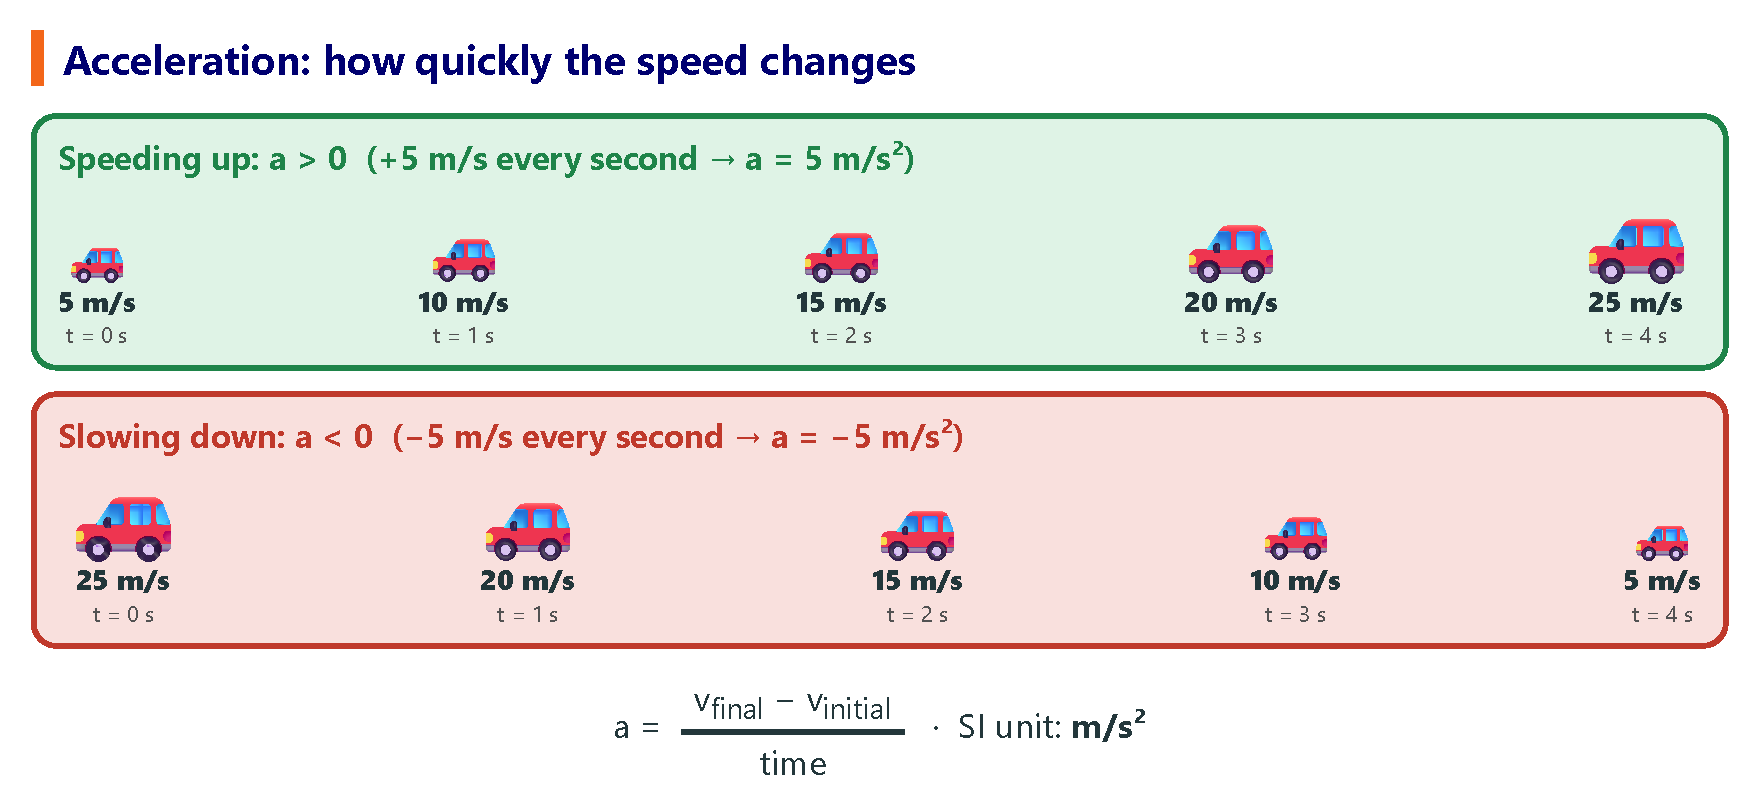
\includegraphics[width=\textwidth]{FigurasSVG/Unit_7_Motion/pdf/acceleration.pdf}
    \caption{Positive acceleration: the speed increases. Negative acceleration: the speed decreases.}
    \label{fig:u7_acceleration}
\end{figure}

\begin{itemize}
    \item If \(a > 0\) (\textbf{positive}), the object speeds up.
    \item If \(a < 0\) (\textbf{negative}), the object slows down.
\end{itemize}

\begin{example}
    \textbf{The speed of a car goes from \qty{5}{\mps} to \qty{25}{\mps} in four seconds. Calculate its acceleration.}
    \begin{equation*}
        a = \dfrac{\qty{25}{\mps} - \qty{5}{\mps}}{\qty{4}{\s}} = \dfrac{\qty{20}{\mps}}{\qty{4}{\s}} = \qty{5}{\mpss}
    \end{equation*}
\end{example}

\begin{exercise}
    A ball rolling at \qty{12}{\mps} decelerates uniformly and comes to a stop after \qty{6}{\s}.
    \begin{enumerate}[label=\letraminuscula]
        \item Calculate its acceleration.
        \item Is the sign of the acceleration what you expected? Explain.
    \end{enumerate}
    \begin{solu}
        \begin{enumerate}[label=\alph*)]
            \item \(a = \dfrac{0 - \qty{12}{\mps}}{\qty{6}{\s}} = \qty{-2}{\mpss}\).
            \item Yes: the acceleration is \textbf{negative} because the ball is slowing down (its speed decreases with time).
        \end{enumerate}
    \end{solu}
\end{exercise}

\begin{exercise}
    An object's speed changes from \(\qty{-4}{\mps}\) to \(\qty{-12}{\mps}\) in \qty{4}{\s} (a negative speed means it is moving towards the origin).
    \begin{enumerate}[label=\letraminuscula]
        \item Calculate the acceleration.
        \item Is the object speeding up or slowing down? Does this match the sign of the acceleration you found in (a)?
    \end{enumerate}
    \begin{solu}
        \begin{enumerate}[label=\alph*)]
            \item \(a = \dfrac{\qty{-12}{\mps} - (\qty{-4}{\mps})}{\qty{4}{\s}} = \dfrac{\qty{-8}{\mps}}{\qty{4}{\s}} = \qty{-2}{\mpss}\).
            \item The object is \textbf{speeding up} (its speed goes from \qty{4}{\mps} to \qty{12}{\mps} in absolute value), even though the acceleration is negative. This shows that the sign of the acceleration tells us the \textbf{direction} in which the speed is changing, not simply whether the object speeds up or slows down: here, both the speed and the acceleration point in the negative direction, so the object speeds up.
        \end{enumerate}
    \end{solu}
\end{exercise}

\subsection{Uniformly accelerated rectilinear motion (UARM)}

\begin{definition}[UARM]
    The motion of an object with a \textbf{straight} trajectory and a \textbf{constant} (non-zero) acceleration: its speed increases, or decreases, by the same amount every second.
\end{definition}

\begin{itemize}
    \item \negsubro{Speed-time graph}: always a straight line. An \textbf{increasing} line means positive acceleration; a \textbf{decreasing} line means negative acceleration. The steeper the line, the greater the (absolute value of the) acceleration.
    \item \negsubro{Distance travelled}: unlike in a URM, the distance travelled in each equal period of time is \textbf{not} the same in a UARM — it increases if \(a>0\), and decreases if \(a<0\).
\end{itemize}

\begin{impt}
    \negsubro{Distance travelled from a speed-time graph, in a UARM}: as in a URM, the distance travelled equals the \textbf{area} between the speed-time line and the time axis. When the object starts from rest (\(v_0 = 0\)), this area is a triangle, so:
    \begin{equation*}
        \text{distance} = \dfrac{v_{\text{final}} \cdot t}{2}
    \end{equation*}
\end{impt}

\begin{figure}[H]
    \centering
    % [FIGURA ORIGINAL] \includegraphics[width=\textwidth]{Unit_7/uarm_graphs}
    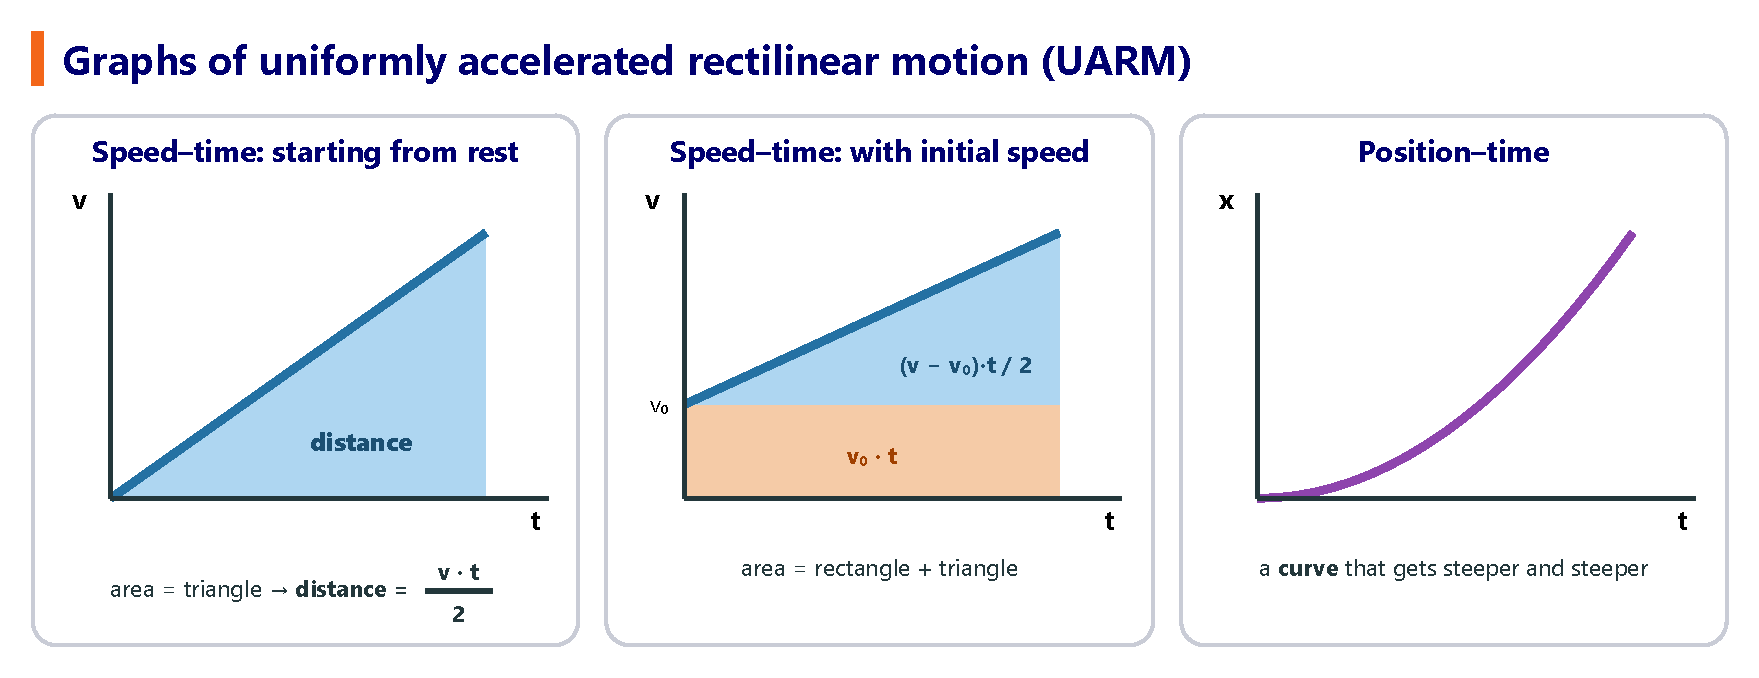
\includegraphics[width=\textwidth]{FigurasSVG/Unit_7_Motion/pdf/uarm_graphs.pdf}
    \caption{Graphs of a UARM: the area under the speed-time graph is the distance travelled.}
    \label{fig:u7_uarm_graphs}
\end{figure}

\begin{example}
    \textbf{A skateboarder starts from rest and speeds up to \qty{6}{\mps} in \qty{4}{\s}, with constant acceleration. Find the acceleration and the distance travelled.}
    \begin{equation*}
        a = \dfrac{\qty{6}{\mps} - 0}{\qty{4}{\s}} = \qty{1.5}{\mpss}
    \end{equation*}
    The speed-time graph is a triangle (a line from \((0,0)\) to \((4,6)\)), so:
    \begin{equation*}
        \text{distance} = \dfrac{v_{\text{final}} \cdot t}{2} = \dfrac{\qty{6}{\mps} \cdot \qty{4}{\s}}{2} = \qty{12}{\m}
    \end{equation*}
\end{example}

\begin{exercise}
    A car starts at \qty{5}{\mps} and accelerates uniformly to \qty{15}{\mps} in \qty{8}{\s}.
    \begin{enumerate}[label=\letraminuscula]
        \item Calculate its acceleration.
        \item The area under its speed-time graph is a trapezium: a rectangle of height \(v_0\) plus a triangle of height \(v_{\text{final}} - v_0\), both with base \(t\). Calculate the distance travelled.
    \end{enumerate}
    \begin{solu}
        \begin{enumerate}[label=\alph*)]
            \item \(a = \dfrac{\qty{15}{\mps} - \qty{5}{\mps}}{\qty{8}{\s}} = \qty{1.25}{\mpss}\).
            \item Rectangle: \(v_0 \cdot t = \qty{5}{\mps} \cdot \qty{8}{\s} = \qty{40}{\m}\). \\
            Triangle: \(\dfrac{(v_{\text{final}}-v_0)\cdot t}{2} = \dfrac{\qty{10}{\mps} \cdot \qty{8}{\s}}{2} = \qty{40}{\m}\). \\
            Total distance \(= 40 + 40 = \qty{80}{\m}\).
        \end{enumerate}
    \end{solu}
\end{exercise}

\begin{exercise}
    A cart starts from rest with a constant acceleration of \qty{2}{\mpss}.
    \begin{enumerate}[label=\letraminuscula]
        \item Complete a table with the speed every second, from \(t=0\) to \(t=4\) s.
        \item Calculate the distance travelled in those \qty{4}{\s}, using the triangle formula.
    \end{enumerate}
    \begin{solu}
        \begin{enumerate}[label=\alph*)]
            \item Since \(v = a \cdot t\):
            \begin{center}
                \begin{tabular}{cccccc}
                    \toprule
                    \(t\) (s) & 0 & 1 & 2 & 3 & 4 \\
                    \midrule
                    \(v\) (m/s) & 0 & 2 & 4 & 6 & 8 \\
                    \bottomrule
                \end{tabular}
            \end{center}
            \item \(\text{distance} = \dfrac{v_{\text{final}} \cdot t}{2} = \dfrac{\qty{8}{\mps} \cdot \qty{4}{\s}}{2} = \qty{16}{\m}\).
        \end{enumerate}
    \end{solu}
\end{exercise}

%\subsection{Free fall: a case of UARM}
%
%\begin{definition}[Free fall]
%    The motion of an object that falls, starting from rest, only under the effect of gravity, with no other force (such as air resistance) acting on it.
%\end{definition}
%
%\begin{figure}[H]
%    \centering
%    \includegraphics[width=0.95\textwidth]{Unit_7/free_fall}
%    \caption{Free fall: the speed increases by about \qty{10}{\mps} every second.}
%    \label{fig:u7_free_fall}
%\end{figure}
%
%\begin{impt}
%    Free fall is a \textbf{UARM} in the vertical direction. Near the Earth's surface, every falling object gains the same speed each second, regardless of its mass: the acceleration due to gravity is
%    \begin{equation*}
%        g \approx \qty{9.8}{\mpss} \quad (\text{often rounded to } \qty{10}{\mpss})
%    \end{equation*}
%    If air resistance is negligible, a heavier object does \textbf{not} fall faster than a lighter one.
%\end{impt}
%
%\begin{example}
%    \textbf{A stone is dropped from a bridge and falls for \qty{2}{\s} before hitting the water. Using \(g = \qty{10}{\mpss}\), find its speed on impact.}
%    \begin{equation*}
%        v = v_0 + g \cdot t = 0 + \qty{10}{\mpss} \cdot \qty{2}{\s} = \qty{20}{\mps}
%    \end{equation*}
%\end{example}
%
%\begin{exercise}
%    A ball is dropped from rest from a window and takes \qty{1.5}{\s} to reach the ground. Using \(g = \qty{10}{\mpss}\), calculate its speed just before hitting the ground.
%    \begin{solu}
%        \(v = v_0 + g \cdot t = 0 + \qty{10}{\mpss} \cdot \qty{1.5}{\s} = \qty{15}{\mps}\).
%    \end{solu}
%\end{exercise}
%
%\begin{exercise}
%    A motorbike starts from rest and accelerates at \qty{8}{\mpss} for the first five seconds.
%    \begin{enumerate}[label=\letraminuscula]
%        \item Make a table with the speed every second, from \(t=0\) to \(t=5\) s.
%    \end{enumerate}
%    \begin{solu}
%        Since \(v = v_0 + a \cdot t\), with \(v_0 = 0\) and \(a = \qty{8}{\mpss}\):
%        \begin{center}
%            \begin{tabular}{ccccccc}
%                \toprule
%                \(t\) (s) & 0 & 1 & 2 & 3 & 4 & 5 \\
%                \midrule
%                \(v\) (m/s) & 0 & 8 & 16 & 24 & 32 & 40 \\
%                \bottomrule
%            \end{tabular}
%        \end{center}
%    \end{solu}
%\end{exercise}
%
%\begin{exercise}
%    A car travelling at \qty{90}{\kmph} brakes and comes to a stop in \qty{10}{\s}.
%    \begin{enumerate}[label=\letraminuscula]
%        \item What was its acceleration?
%    \end{enumerate}
%    \begin{solu}
%        First convert the speed: \(\qty{90}{\kmph} = \qty{25}{\mps}\). \\
%        \(a = \dfrac{v_{\text{final}} - v_{\text{initial}}}{t} = \dfrac{0 - \qty{25}{\mps}}{\qty{10}{\s}} = \qty{-2.5}{\mpss}\) (negative, since the car slows down).
%    \end{solu}
%\end{exercise}
%
%\begin{exercise}
%    A cyclist moving at \qty{4}{\mps} accelerates uniformly at \qty{0.5}{\mpss} for \qty{6}{\s}.
%    \begin{enumerate}[label=\letraminuscula]
%        \item Calculate her final speed.
%        \item Sketch, in words, the shape of her speed-time graph and the shape of her distance-time graph (increasing/decreasing, straight/curved).
%    \end{enumerate}
%    \begin{solu}
%        \begin{enumerate}[label=\alph*)]
%            \item \(v_{\text{final}} = v_{\text{initial}} + a \cdot t = \qty{4}{\mps} + \qty{0.5}{\mpss} \cdot \qty{6}{\s} = \qty{7}{\mps}\).
%            \item The speed-time graph is a \textbf{straight, increasing} line (constant positive acceleration), starting at \(v=\qty{4}{\mps}\) instead of at zero. The position-time graph is \textbf{curved}, becoming steeper and steeper, because the speed (and therefore the distance covered per second) keeps increasing.
%        \end{enumerate}
%    \end{solu}
%\end{exercise}
%
%\begin{exercise}
%    A stone is dropped from rest and hits the ground after \qty{3}{\s}. Using \(g=\qty{10}{\mpss}\):
%    \begin{enumerate}[label=\letraminuscula]
%        \item Calculate its speed on impact.
%        \item Calculate the height from which it was dropped, using the triangle formula for the distance travelled.
%    \end{enumerate}
%    \begin{solu}
%        \begin{enumerate}[label=\alph*)]
%            \item \(v = v_0 + g \cdot t = 0 + \qty{10}{\mpss} \cdot \qty{3}{\s} = \qty{30}{\mps}\).
%            \item \(\text{height} = \dfrac{v_{\text{final}} \cdot t}{2} = \dfrac{\qty{30}{\mps} \cdot \qty{3}{\s}}{2} = \qty{45}{\m}\).
%        \end{enumerate}
%    \end{solu}
%\end{exercise}
%
%%----------------------------------------------------------------------------------------
%
%\section{Uniform circular motion (UCM)}
%
%\begin{definition}[Uniform circular motion (UCM)]
%    The motion of an object whose trajectory is a \textbf{circumference} and whose speed is \textbf{constant}.
%\end{definition}
%
%A UCM is a \textbf{periodic} motion, since it repeats at regular intervals of time.
%
%\begin{itemize}
%    \item \negsubro{Period}, \(T\): the time it takes the object to complete one full rotation.
%    \item \negsubro{Frequency}, \(f\): the number of rotations completed in a certain time; it is the inverse of the period. The greater the period, the lower the frequency.
%    \begin{equation*}
%        f = \dfrac{1}{T}
%    \end{equation*}
%\end{itemize}
%
%\begin{example}
%    The hour hand of a clock completes 1 rotation every 12 hours; the minute hand, 1 rotation every hour; the second hand, 1 rotation every minute. The hour hand has the \textbf{longest} period and the \textbf{lowest} frequency of the three.
%\end{example}
%
%\begin{example}
%    \textbf{The Earth rotates on its axis once a day. A point on the Equator (circumference length \qty{40077}{\km}) and a point on the Arctic Circle (circumference length \qty{15996}{\km}) both complete one rotation a day. Compare their periods, frequencies and speeds.}
%
%    Both points have the \textbf{same period} (\(T = \qty{24}{\hour}\)) and the \textbf{same frequency}, since they both complete one rotation per day. However, their \textbf{speeds} are different, because they travel different distances (different circumference lengths) in the same time:
%    \begin{equation*}
%        v_{\text{Equator}} = \dfrac{\qty{40077}{\km}}{\qty{24}{\hour}} \approx \qty{1670}{\kmph}
%        \qquad
%        v_{\text{Arctic Circle}} = \dfrac{\qty{15996}{\km}}{\qty{24}{\hour}} \approx \qty{666.5}{\kmph}
%    \end{equation*}
%\end{example}
%
%\begin{exercise}
%    Order the hour hand, minute hand and second hand of a clock by their period, from shortest to longest.
%    \begin{solu}
%        Second hand (\(T = \qty{1}{\minute}\)) \(<\) minute hand (\(T = \qty{1}{\hour}\)) \(<\) hour hand (\(T = \qty{12}{\hour}\)).
%    \end{solu}
%\end{exercise}
%
%\begin{exercise}
%    A fan blade completes 300 rotations per minute.
%    \begin{enumerate}[label=\letraminuscula]
%        \item Calculate its frequency, in \unit{\hertz}.
%        \item Calculate its period.
%    \end{enumerate}
%    \begin{solu}
%        \begin{enumerate}[label=\alph*)]
%            \item \(f = \dfrac{300 \text{ rotations}}{\qty{60}{\s}} = \qty{5}{\hertz}\).
%            \item \(T = \dfrac{1}{f} = \dfrac{1}{\qty{5}{\hertz}} = \qty{0.2}{\s}\).
%        \end{enumerate}
%    \end{solu}
%\end{exercise}
%
%\begin{exercise}
%    Wheel \(A\) has a period of \qty{0.5}{\s}. Wheel \(B\) completes 4 rotations every \qty{3}{\s}.
%    \begin{enumerate}[label=\letraminuscula]
%        \item Calculate the frequency of each wheel.
%        \item Which wheel is rotating faster?
%    \end{enumerate}
%    \begin{solu}
%        \begin{enumerate}[label=\alph*)]
%            \item \(f_A = \dfrac{1}{T_A} = \dfrac{1}{\qty{0.5}{\s}} = \qty{2}{\hertz}\). \\
%            \(f_B = \dfrac{4 \text{ rotations}}{\qty{3}{\s}} \approx \qty{1.33}{\hertz}\).
%            \item Since \(f_A > f_B\), \textbf{wheel \(A\)} completes more rotations per second, so it is rotating faster.
%        \end{enumerate}
%    \end{solu}
%\end{exercise}
%
%\subsection{Linear speed in UCM}
%
%\begin{definition}[Linear (tangential) speed in UCM]
%    In one period, an object in UCM travels a distance equal to the circumference length, \(2\pi r\), where \(r\) is the radius of the circular trajectory. Its (constant) linear speed is therefore:
%    \begin{equation*}
%        v = \dfrac{2\pi r}{T} = 2\pi r \cdot f
%    \end{equation*}
%\end{definition}
%
%\begin{figure}[H]
%    \centering
%    \includegraphics[width=\textwidth]{Unit_7/ucm}
%    \caption{Uniform circular motion: period, frequency and linear speed.}
%    \label{fig:u7_ucm}
%\end{figure}
%
%\begin{example}
%    \textbf{A carousel horse moves in a circle of radius \qty{4}{\m}, completing one turn every \qty{8}{\s}. Calculate its linear speed.}
%    \begin{equation*}
%        v = \dfrac{2\pi \cdot \qty{4}{\m}}{\qty{8}{\s}} \approx \qty{3.14}{\mps}
%    \end{equation*}
%\end{example}
%
%\begin{exercise}
%    A point on the rim of a bicycle wheel of radius \qty{0.35}{\m} completes 2 rotations per second.
%    \begin{enumerate}[label=\letraminuscula]
%        \item Calculate the period of its motion.
%        \item Calculate its linear speed.
%    \end{enumerate}
%    \begin{solu}
%        \begin{enumerate}[label=\alph*)]
%            \item \(T = \dfrac{1}{f} = \dfrac{1}{\qty{2}{\hertz}} = \qty{0.5}{\s}\).
%            \item \(v = 2\pi r \cdot f = 2\pi \cdot \qty{0.35}{\m} \cdot \qty{2}{\hertz} \approx \qty{4.4}{\mps}\).
%        \end{enumerate}
%    \end{solu}
%\end{exercise}
%
%\begin{exercise}
%    A satellite orbits the Earth in a circle of radius \qty{7000}{\km}, completing one orbit every \qty{2}{\hour}.
%    \begin{enumerate}[label=\letraminuscula]
%        \item Calculate its linear speed, in \unit{\kmph}.
%    \end{enumerate}
%    \begin{solu}
%        \(v = \dfrac{2\pi r}{T} = \dfrac{2\pi \cdot \qty{7000}{\km}}{\qty{2}{\hour}} \approx \qty{21991}{\kmph}\).
%    \end{solu}
%\end{exercise}
%
%\begin{exercise}
%    A point on a spinning disc of radius \qty{0.2}{\m} has a linear speed of \qty{4}{\mps}.
%    \begin{enumerate}[label=\letraminuscula]
%        \item Calculate its period.
%        \item Calculate its frequency.
%    \end{enumerate}
%    \begin{solu}
%        \begin{enumerate}[label=\alph*)]
%            \item From \(v = \dfrac{2\pi r}{T}\), we get \(T = \dfrac{2\pi r}{v} = \dfrac{2\pi \cdot \qty{0.2}{\m}}{\qty{4}{\mps}} \approx \qty{0.31}{\s}\).
%            \item \(f = \dfrac{1}{T} \approx \dfrac{1}{\qty{0.31}{\s}} \approx \qty{3.18}{\hertz}\).
%        \end{enumerate}
%    \end{solu}
%\end{exercise}

%----------------------------------------------------------------------------------------

\section*{Summary}

\begin{itemize}
    \item \textbf{Motion is relative} to the chosen frame of reference. Key quantities: position (\(x\)), trajectory, distance travelled and displacement.
    \item \textbf{Speed} \(= \) distance / time (SI unit: \unit{\mps}). Average speed uses the whole journey; instantaneous speed is read at one moment.
    \item \textbf{URM}: constant speed, straight trajectory; position-time graph is a straight line; speed-time graph is a horizontal line; distance = area under the speed-time graph.
    \item \textbf{Acceleration} \(=\) change in speed / time (SI unit: \unit{\mpss}). \textbf{UARM}: constant acceleration, straight trajectory; the distance travelled per equal time interval changes; distance = area under the speed-time graph (a triangle, if starting from rest).
    \item \textbf{Free fall} is a UARM with \(a = g \approx \qty{9.8}{\mpss}\), the same for every object regardless of its mass (if air resistance is negligible).
    \item \textbf{UCM}: circular trajectory, constant speed; described by the period \(T\) (time per rotation) and the frequency \(f = 1/T\); linear speed \(v = 2\pi r / T\).
\end{itemize}

\section{Vocabulary}

\begin{vocabulary}[Frame of reference]
    A fixed point, or set of points, used to describe the position and motion of a body. \newline
    \textbf{Translation to Spanish}: Sistema de referencia
\end{vocabulary}

\begin{vocabulary}[Trajectory]
    The line followed by a moving object. \newline
    \textbf{Translation to Spanish}: Trayectoria
\end{vocabulary}

\begin{vocabulary}[Displacement]
    The shortest distance between the initial and final position of a moving object. \newline
    \textbf{Translation to Spanish}: Desplazamiento
\end{vocabulary}

\begin{vocabulary}[Speed]
    A quantity that measures how fast an object moves; distance travelled per unit of time. \newline
    \textbf{Translation to Spanish}: Rapidez / velocidad
\end{vocabulary}

\begin{vocabulary}[Acceleration]
    A quantity that measures the change in speed per unit of time. \newline
    \textbf{Translation to Spanish}: Aceleración
\end{vocabulary}

\begin{vocabulary}[Uniform rectilinear motion]
    Motion with a straight trajectory and constant speed. \newline
    \textbf{Translation to Spanish}: Movimiento rectilíneo uniforme
\end{vocabulary}

\begin{vocabulary}[Uniform circular motion]
    Motion with a circular trajectory and constant speed. \newline
    \textbf{Translation to Spanish}: Movimiento circular uniforme
\end{vocabulary}

\begin{vocabulary}[Period]
    The time an object takes to complete one full rotation, in a periodic motion. \newline
    \textbf{Translation to Spanish}: Periodo
\end{vocabulary}

\begin{vocabulary}[Frequency]
    The number of rotations completed per unit of time. \newline
    \textbf{Translation to Spanish}: Frecuencia
\end{vocabulary}

\begin{vocabulary}[Free fall]
    The motion of an object falling from rest under the effect of gravity alone. \newline
    \textbf{Translation to Spanish}: Caída libre
\end{vocabulary}



%------------------------------------------------


    \chapterimage{images/portada_cabeceras/cabecera_Unit8}
    \chapter{Forces}
    % Saberes básicos (LOMLOE) asociados a esta unidad
%
% D. La interacción
%   - Las fuerzas como agentes de cambio: relación de los efectos de las fuerzas, tanto en el
%     estado de movimiento o de reposo de un cuerpo como produciendo deformaciones en los
%     sistemas sobre los que actúan: se trata explícitamente en "Forces and motion. Newton's
%     laws" y en "Forces and deformation" (cuerpos rígidos, elásticos y plásticos, ley de Hooke).
%   - Aplicación de las leyes de Newton: observación de situaciones cotidianas o de laboratorio
%     que permiten entender cómo se comportan los sistemas materiales ante la acción de las
%     fuerzas y predecir los efectos de estas en situaciones cotidianas y de seguridad vial:
%     las tres leyes de Newton se presentan con ejemplos cotidianos (patinadores, coches,
%     cinturón de seguridad) y se añade un apartado específico de fricción y seguridad vial
%     (distancia de frenado, cinturón de seguridad, airbag, distancia de seguridad).
%   - Fenómenos gravitatorios: el peso como fuerza de atracción gravitatoria se relaciona con
%     la masa y con las leyes de Newton (segunda ley aplicada a la caída libre).
%
% A. Las destrezas científicas básicas
%   - Unidades del Sistema Internacional: uso sistemático de \unit{} y \qty{} (N, N/m, m/s^2).
%
% (Unidad separada de la antigua «Forces and Motion»: la cinemática está en la Unidad 7, Motion.)

\spacing{1.3}
\raggedbottom % pages with large figures end where the text ends (no stretched gaps between boxes)

\section{Introduction}

In the previous unit we learnt to describe motion. In this unit we will study its cause: \textbf{forces}. We will see what a force is, how \textbf{Newton's laws} explain the way forces change the motion of bodies, the difference between \textbf{weight} and \textbf{mass}, and how forces can also \textbf{deform} objects.

\section{Forces and motion. Newton's laws}

\subsection{What is a force?}

\begin{definition}[Force]
    Any action capable of \textbf{changing the state of motion} of a body (making it start moving, stop, speed up, slow down or change direction) or of \textbf{deforming} it. It is represented by the letter \(F\) and, in the SI, it is measured in \textbf{newtons} (\unit{\newton}).
\end{definition}

\begin{impt}
    \negsubro{Forces are the cause of changes in motion}:
    \begin{itemize}
        \item Forces are what make objects \textbf{start moving}, and what make them \textbf{speed up, slow down, stop or turn}.
        \item If \textbf{no force} acts on an object (or all the forces cancel each other out), the object \textbf{does not move} if it was at rest, or it keeps moving \textbf{at a constant velocity} in a straight line. In both cases its velocity does not change, so its \textbf{acceleration is zero} (\(a = 0\)).
    \end{itemize}
\end{impt}

\begin{definition}[Newton, N]
    The SI unit of force. A force of \qty{1}{\newton} acting on a \qty{1}{\kg} object produces an acceleration of \qty{1}{\mpss}, in the same direction as the force.
\end{definition}

The British scientist Isaac Newton (1642--1727) discovered three laws that explain how forces change the motion of objects.

\begin{figure}[H]
    \centering
    % [FIGURA ORIGINAL] \includegraphics[width=\textwidth]{Unit_8/newton_laws}
    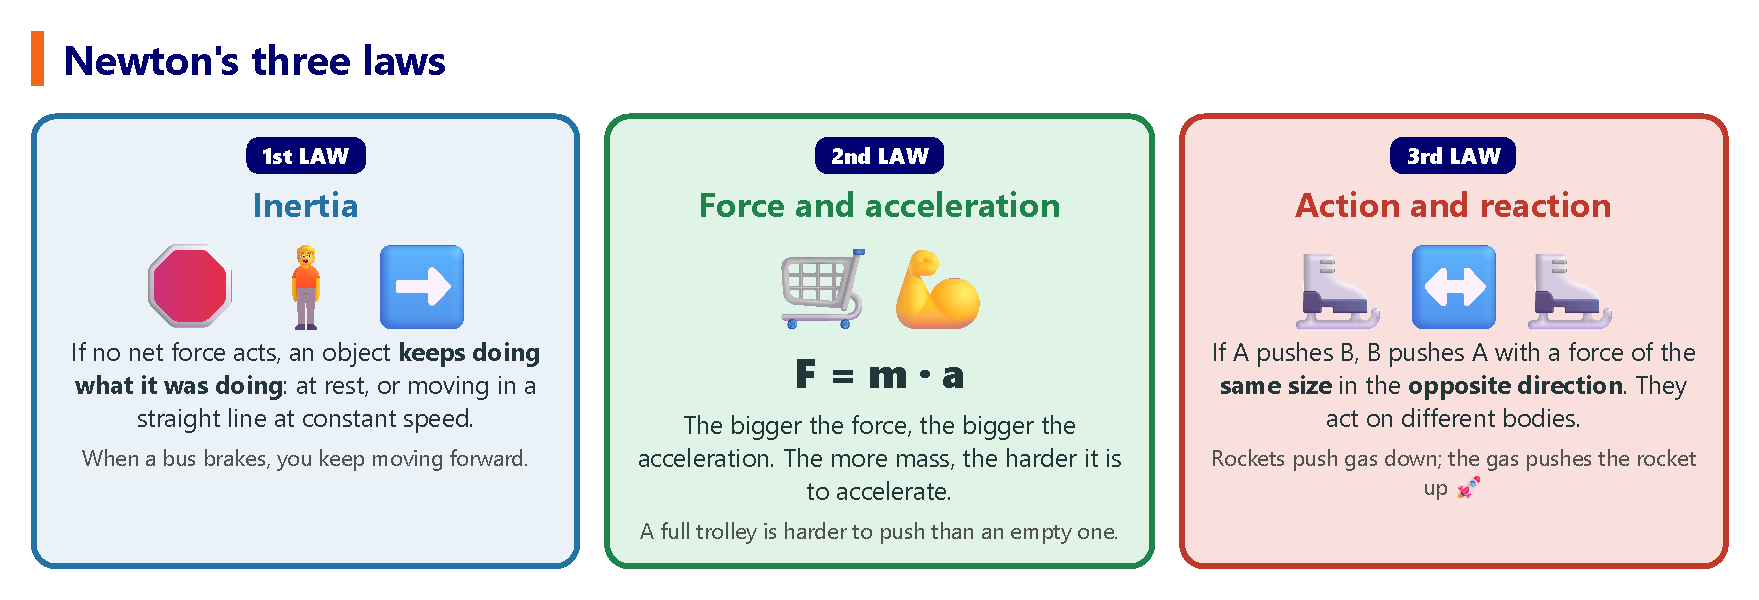
\includegraphics[width=\textwidth]{FigurasSVG/Unit_8_Forces/pdf/newton_laws.pdf}
    \caption{Newton's three laws of motion.}
    \label{fig:u8_newton_laws}
\end{figure}

\subsection{Newton's first law: the law of inertia}

\begin{definition}[Newton's first law]
    If no force acts on a body (or the forces acting on it cancel out), the body stays \textbf{at rest} if it was at rest, or keeps moving in a \textbf{straight line at a constant velocity} (URM) if it was moving.
\end{definition}

Bodies ``prefer'' to keep doing what they were doing: this tendency to resist changes in their motion is called \negsubro{inertia}. The more mass a body has, the more inertia it has: it is harder to start pushing a car than a bicycle, and harder to stop it.

\begin{example}
    \begin{itemize}
        \item When a bus brakes suddenly, the passengers lurch \textbf{forwards}: their bodies tend to keep moving at the speed the bus had.
        \item When a bus starts suddenly, the passengers lurch \textbf{backwards}: their bodies tend to stay at rest.
        \item A hockey puck slides a long way on the ice, because there is almost no friction to stop it.
    \end{itemize}
\end{example}

\subsection{Newton's second law: the fundamental law of dynamics}

\begin{definition}[Newton's second law]
    When a (net) force acts on a body, it produces an \textbf{acceleration} in the same direction as the force. The force is equal to the mass of the body multiplied by its acceleration:
    \begin{equation*}
        F = m \cdot a
    \end{equation*}
    where \(F\) is the force (\unit{\newton}), \(m\) the mass (\unit{\kg}) and \(a\) the acceleration (\unit{\mpss}).
\end{definition}

\begin{impt}
    \begin{itemize}
        \item The \textbf{bigger the force}, the \textbf{bigger the acceleration}: if we push harder, the object speeds up more.
        \item The \textbf{bigger the mass}, the \textbf{smaller the acceleration}: with the same push, an empty trolley speeds up more than a full one.
        \item If the force is zero, the acceleration is zero: this is the first law again.
    \end{itemize}
\end{impt}

In the exercises we may be asked for the force, the mass or the acceleration. To calculate \(m\) or \(a\), we first \textbf{isolate} them, as we did with density and velocity:

\begin{figure}[H]
    \centering
    % [FIGURA ORIGINAL] \includegraphics[width=\textwidth]{Unit_8/newton2_isolate}
    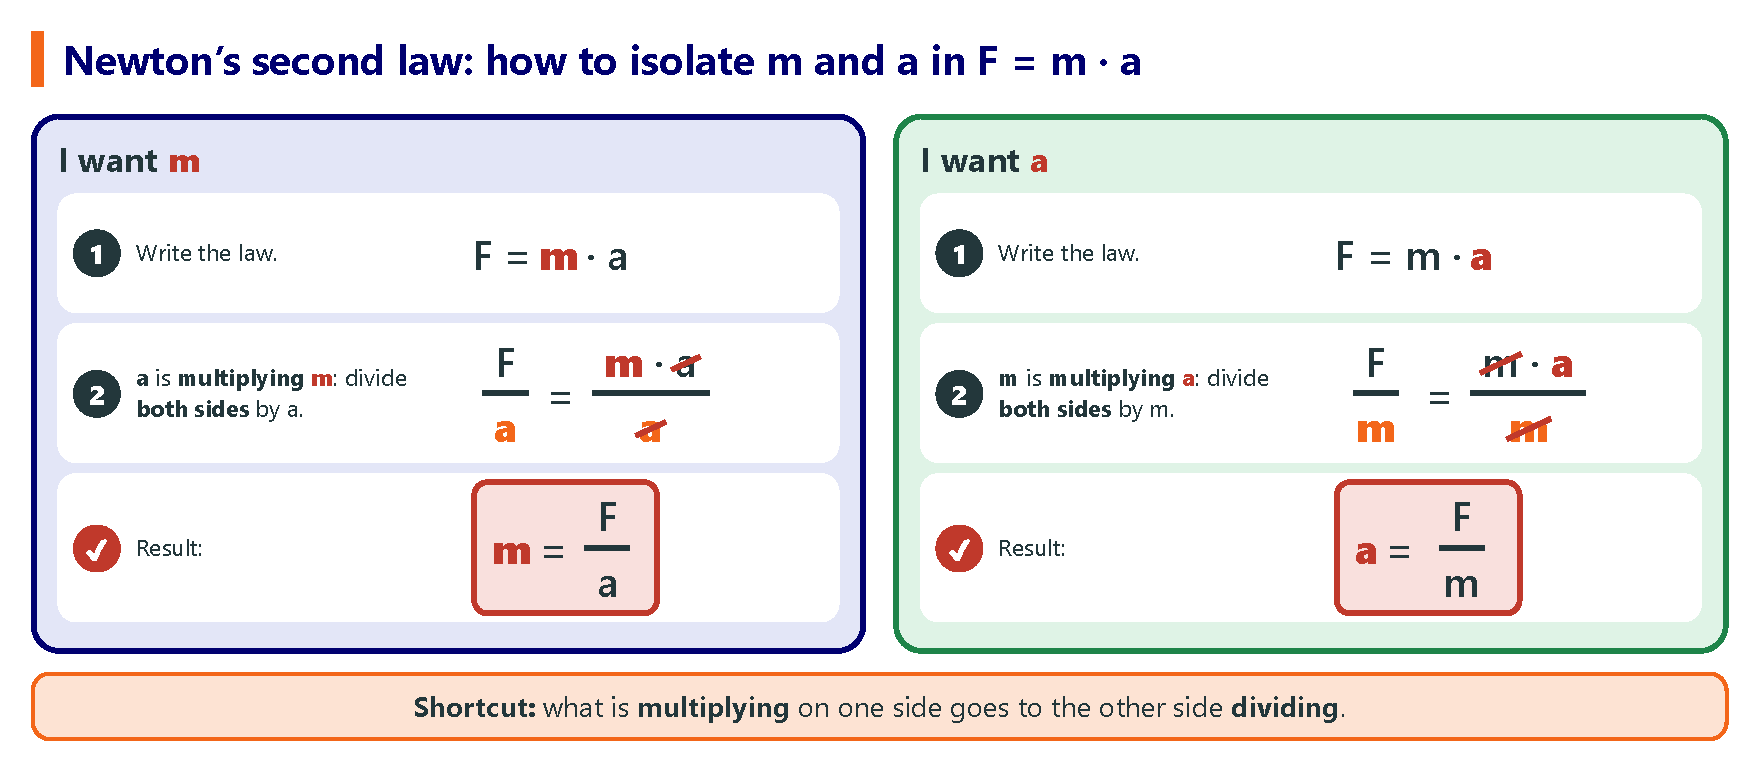
\includegraphics[width=\textwidth]{FigurasSVG/Unit_8_Forces/pdf/newton2_isolate.pdf}
    \caption{Isolating the mass and the acceleration in \(F = m \cdot a\), step by step.}
    \label{fig:u8_newton2_isolate}
\end{figure}

\begin{itemize}
    \item \textbf{Mass}: \(a\) is multiplying \(m\), so we divide both sides by \(a\):
    \(\;\dfrac{F}{a} = \dfrac{m \cdot \cancelred{a}}{\cancelred{a}} \;\Rightarrow\; \textcolor{red}{m = \dfrac{F}{a}}\)
    \item \textbf{Acceleration}: \(m\) is multiplying \(a\), so we divide both sides by \(m\):
    \(\;\dfrac{F}{m} = \dfrac{\cancelred{m} \cdot a}{\cancelred{m}} \;\Rightarrow\; \textcolor{red}{a = \dfrac{F}{m}}\)
\end{itemize}

\begin{impt}
    The three versions of Newton's second law:
    \begin{equation*}
        F = m \cdot a \qquad\qquad m = \dfrac{F}{a} \qquad\qquad a = \dfrac{F}{m}
    \end{equation*}
\end{impt}

\begin{example}
    \textbf{Calculating a force. What force is needed to give a \qty{50}{\kg} trolley an acceleration of \qty{2}{\mpss}?}
    \begin{enumerate}[label=\numberballmDarkTeal]
        \item Data: \(m = \qty{50}{\kg}\), \(a = \qty{2}{\mpss}\). Unknown: \(\underline{F}\).
        \item Formula: \(F = m \cdot a\) (no need to isolate).
        \item \(F = \qty{50}{\kg} \cdot \qty{2}{\mpss} = \textcolor{red}{\qty{100}{\newton}}\).
    \end{enumerate}
\end{example}

\begin{example}
    \textbf{Calculating a mass. A force of \qty{300}{\newton} gives a motorbike an acceleration of \qty{1.5}{\mpss}. What is the mass of the motorbike?}
    \begin{enumerate}[label=\numberballmDarkTeal]
        \item Data: \(F = \qty{300}{\newton}\), \(a = \qty{1.5}{\mpss}\). Unknown: \(\underline{m}\).
        \item Formula: \(F = m \cdot a\). \(a\) is multiplying \(m\), so it goes to the other side dividing: \(m = \dfrac{F}{a}\).
        \item \(m = \dfrac{\qty{300}{\newton}}{\qty{1.5}{\mpss}} = \textcolor{red}{\qty{200}{\kg}}\).
    \end{enumerate}
\end{example}

\begin{example}
    \textbf{Calculating an acceleration. A force of \qty{60}{\newton} pushes a \qty{12}{\kg} box. What acceleration does it get?}
    \begin{enumerate}[label=\numberballmDarkTeal]
        \item Data: \(F = \qty{60}{\newton}\), \(m = \qty{12}{\kg}\). Unknown: \(\underline{a}\).
        \item Formula: \(F = m \cdot a\). \(m\) is multiplying \(a\), so it goes to the other side dividing: \(a = \dfrac{F}{m}\).
        \item \(a = \dfrac{\qty{60}{\newton}}{\qty{12}{\kg}} = \textcolor{red}{\qty{5}{\mpss}}\).
    \end{enumerate}
\end{example}

\begin{exercise}
    \textbf{Calculate the force} in each case:
    \begin{enumerate}[label=\letraminuscula]
        \item A \qty{1200}{\kg} car accelerates at \qty{3}{\mpss}.
        \item A \qty{0.45}{\kg} football is kicked and gets an acceleration of \qty{200}{\mpss}.
        \item A \qty{70}{\kg} cyclist (with her bike) accelerates at \qty{0.5}{\mpss}.
    \end{enumerate}
    \begin{solu}
        \begin{enumerate}[label=\alph*)]
            \item \(F = m \cdot a = \qty{1200}{\kg} \cdot \qty{3}{\mpss} = \qty{3600}{\newton}\).
            \item \(F = \qty{0.45}{\kg} \cdot \qty{200}{\mpss} = \qty{90}{\newton}\).
            \item \(F = \qty{70}{\kg} \cdot \qty{0.5}{\mpss} = \qty{35}{\newton}\).
        \end{enumerate}
    \end{solu}
\end{exercise}

\begin{exercise}
    \textbf{Calculate the mass} in each case:
    \begin{enumerate}[label=\letraminuscula]
        \item A force of \qty{20}{\newton} produces an acceleration of \qty{4}{\mpss}.
        \item A force of \qty{4500}{\newton} gives a van an acceleration of \qty{1.5}{\mpss}.
        \item A force of \qty{9}{\newton} gives a skateboard an acceleration of \qty{3}{\mpss}.
    \end{enumerate}
    \begin{solu}
        \begin{enumerate}[label=\alph*)]
            \item \(m = \dfrac{F}{a} = \dfrac{\qty{20}{\newton}}{\qty{4}{\mpss}} = \qty{5}{\kg}\).
            \item \(m = \dfrac{\qty{4500}{\newton}}{\qty{1.5}{\mpss}} = \qty{3000}{\kg}\).
            \item \(m = \dfrac{\qty{9}{\newton}}{\qty{3}{\mpss}} = \qty{3}{\kg}\).
        \end{enumerate}
    \end{solu}
\end{exercise}

\begin{exercise}
    \textbf{Calculate the acceleration} in each case:
    \begin{enumerate}[label=\letraminuscula]
        \item A force of \qty{40}{\newton} acts on a \qty{8}{\kg} sledge.
        \item A force of \qty{2000}{\newton} acts on a \qty{500}{\kg} boat.
        \item A force of \qty{15}{\newton} acts on a \qty{0.5}{\kg} ball.
    \end{enumerate}
    \begin{solu}
        \begin{enumerate}[label=\alph*)]
            \item \(a = \dfrac{F}{m} = \dfrac{\qty{40}{\newton}}{\qty{8}{\kg}} = \qty{5}{\mpss}\).
            \item \(a = \dfrac{\qty{2000}{\newton}}{\qty{500}{\kg}} = \qty{4}{\mpss}\).
            \item \(a = \dfrac{\qty{15}{\newton}}{\qty{0.5}{\kg}} = \qty{30}{\mpss}\).
        \end{enumerate}
    \end{solu}
\end{exercise}

\begin{exercise}
    Calculate the acceleration produced on an object of mass \qty{2}{\kg} by a force of \qty{5}{\newton}.
    \begin{enumerate}[label=\letraminuscula]
        \item What force would we need to apply to a \qty{10}{\kg} object to produce the same acceleration?
    \end{enumerate}
    \begin{solu}
        \(a = \dfrac{F}{m} = \dfrac{\qty{5}{\newton}}{\qty{2}{\kg}} = \qty{2.5}{\mpss}\). \\
        For the same acceleration on \qty{10}{\kg}: \(F = m \cdot a = \qty{10}{\kg} \cdot \qty{2.5}{\mpss} = \qty{25}{\newton}\).
    \end{solu}
\end{exercise}

\begin{exercise}
    A car of mass \qty{1000}{\kg} has an engine force of \qty{2000}{\newton} and a frictional force of \qty{1500}{\newton} acting against it. Calculate its acceleration.
    \begin{solu}
        Net force \(= \qty{2000}{\newton} - \qty{1500}{\newton} = \qty{500}{\newton}\) (in the direction of motion). \\
        \(a = \dfrac{F}{m} = \dfrac{\qty{500}{\newton}}{\qty{1000}{\kg}} = \qty{0.5}{\mpss}\).
    \end{solu}
\end{exercise}

\begin{exercise}
    A net force of \qty{12}{\newton} acting on an object produces an acceleration of \qty{3}{\mpss}.
    \begin{enumerate}[label=\letraminuscula]
        \item Calculate the mass of the object.
        \item If the same object were pushed with a net force of \qty{24}{\newton}, what acceleration would it have?
    \end{enumerate}
    \begin{solu}
        \begin{enumerate}[label=\alph*)]
            \item \(m = \dfrac{F}{a} = \dfrac{\qty{12}{\newton}}{\qty{3}{\mpss}} = \qty{4}{\kg}\).
            \item \(a = \dfrac{F}{m} = \dfrac{\qty{24}{\newton}}{\qty{4}{\kg}} = \qty{6}{\mpss}\).
        \end{enumerate}
    \end{solu}
\end{exercise}


\subsection{Newton's third law: action and reaction}

\begin{definition}[Newton's third law]
    When a body exerts a force on another body (\textbf{action}), the second body exerts on the first a force of the \textbf{same value} but in the \textbf{opposite direction} (\textbf{reaction}).
\end{definition}

\begin{impt}
    Forces always come in \textbf{pairs}. The action and the reaction act on \textbf{different bodies}, so they \textbf{do not cancel} each other out.
\end{impt}

\begin{example}
    A skater pushes another skater. Both skaters move backwards: the push is the \textbf{action}, and the force that pushes the first skater back is the \textbf{reaction}. The two forces have the same value but opposite directions, and act on different people, so they do not cancel out.
\end{example}

\begin{example}
    \begin{itemize}
        \item \textbf{Walking}: our foot pushes the ground backwards (action), and the ground pushes us forwards (reaction).
        \item \textbf{Swimming}: we push the water backwards with our hands, and the water pushes us forwards.
        \item \textbf{A rocket}: it pushes the gases downwards, and the gases push the rocket upwards.
    \end{itemize}
\end{example}

\begin{impt}
    \negsubro{Relating forces and motion}:
    \begin{itemize}
        \item No net force acts \(\to\) object stays \textbf{at rest} or keeps its \textbf{URM} (\(a = 0\)).
        \item A net force changes the \textbf{value} of the velocity, uniformly \(\to\) \textbf{UARM}.
        \item A net force changes only the \textbf{direction} of motion (not the speed) \(\to\) \textbf{circular motion}.
    \end{itemize}
\end{impt}

\subsection{Weight and mass}

\begin{impt}
    \negsubro{Weight is a force}: it is the force with which a celestial body (such as the Earth) attracts a mass towards its centre. It should not be confused with mass:
    \begin{itemize}
        \item \textbf{Mass} (\(m\)): the amount of matter in a body. It is measured in \unit{\kg} and does \textbf{not} change from place to place.
        \item \textbf{Weight} (\(W\)): the force of gravity acting on that mass. It is measured in \unit{\newton} and \textbf{does} change: it is different on the Moon than on Earth.
    \end{itemize}
\end{impt}

\begin{definition}[Weight]
    The weight of an object equals its mass times the acceleration due to gravity, applying Newton's second law:
    \begin{equation*}
        W = m \cdot g
    \end{equation*}
    On Earth, \(g \approx \qty{9.8}{\mpss}\) (often rounded to \qty{10}{\mpss}).
\end{definition}

\begin{figure}[H]
    \centering
    % [FIGURA ORIGINAL] \includegraphics[width=\textwidth]{Unit_8/weight_planets}
    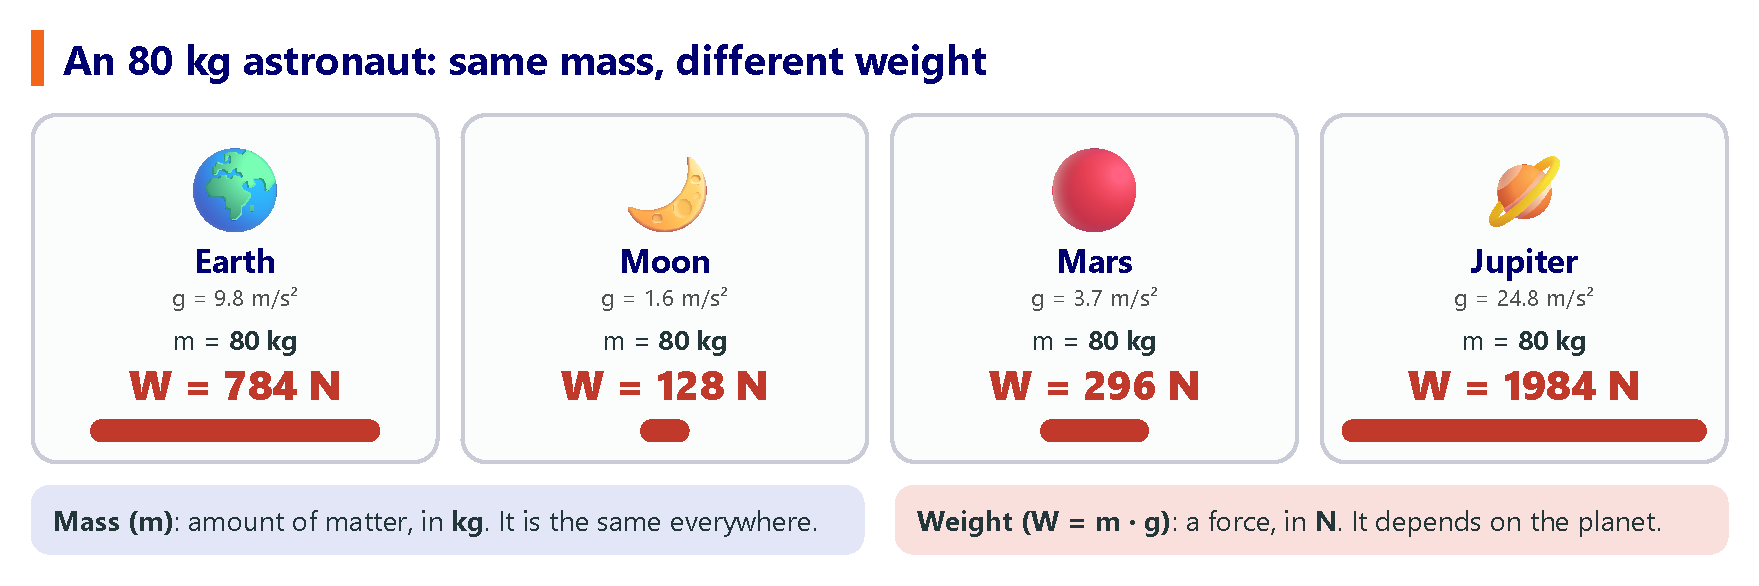
\includegraphics[width=\textwidth]{FigurasSVG/Unit_8_Forces/pdf/weight_planets.pdf}
    \caption{The mass of the astronaut is the same everywhere; the weight depends on the gravity of each place.}
    \label{fig:u8_weight_planets}
\end{figure}

\begin{example}
    \textbf{Calculate the weight of a \qty{60}{\kg} student on Earth (\(g=\qty{9.8}{\mpss}\)) and on the Moon (\(g_{\text{Moon}} \approx \qty{1.6}{\mpss}\)).}
    \begin{equation*}
        W_{\text{Earth}} = \qty{60}{\kg} \cdot \qty{9.8}{\mpss} = \qty{588}{\newton}
        \qquad
        W_{\text{Moon}} = \qty{60}{\kg} \cdot \qty{1.6}{\mpss} = \qty{96}{\newton}
    \end{equation*}
    The student's \textbf{mass} (\qty{60}{\kg}) is the same in both places; only the \textbf{weight} changes, because \(g\) is different.
\end{example}

\begin{exercise}
    An astronaut has a mass of \qty{80}{\kg}.
    \begin{enumerate}[label=\letraminuscula]
        \item Calculate her weight on Earth (\(g=\qty{9.8}{\mpss}\)).
        \item Calculate her weight on Mars, where \(g_{\text{Mars}} \approx \qty{3.7}{\mpss}\).
        \item Does her mass change between Earth and Mars?
    \end{enumerate}
    \begin{solu}
        \begin{enumerate}[label=\alph*)]
            \item \(W_{\text{Earth}} = \qty{80}{\kg} \cdot \qty{9.8}{\mpss} = \qty{784}{\newton}\).
            \item \(W_{\text{Mars}} = \qty{80}{\kg} \cdot \qty{3.7}{\mpss} = \qty{296}{\newton}\).
            \item No: her \textbf{mass} stays at \qty{80}{\kg} on both planets; only her \textbf{weight} changes, because it depends on \(g\).
        \end{enumerate}
    \end{solu}
\end{exercise}

\begin{exercise}
    A box weighs \qty{500}{\newton} on Earth (\(g=\qty{10}{\mpss}\)).
    \begin{enumerate}[label=\letraminuscula]
        \item Calculate its mass.
        \item Calculate its weight on the Moon (\(g_{\text{Moon}} \approx \qty{1.6}{\mpss}\)).
    \end{enumerate}
    \begin{solu}
        \begin{enumerate}[label=\alph*)]
            \item \(m = \dfrac{W}{g} = \dfrac{\qty{500}{\newton}}{\qty{10}{\mpss}} = \qty{50}{\kg}\).
            \item \(W_{\text{Moon}} = m \cdot g_{\text{Moon}} = \qty{50}{\kg} \cdot \qty{1.6}{\mpss} = \qty{80}{\newton}\).
        \end{enumerate}
    \end{solu}
\end{exercise}

\begin{exercise}
    Object \(X\) has a mass of \qty{10}{\kg} and object \(Y\) has a mass of \qty{20}{\kg}. Both are taken to Jupiter, where \(g_{\text{Jupiter}} \approx \qty{24.8}{\mpss}\).
    \begin{enumerate}[label=\letraminuscula]
        \item Calculate the weight of each object on Jupiter.
        \item Which object weighs more? Would this still be true if we compared them on Earth instead?
    \end{enumerate}
    \begin{solu}
        \begin{enumerate}[label=\alph*)]
            \item \(W_X = \qty{10}{\kg} \cdot \qty{24.8}{\mpss} = \qty{248}{\newton}\). \\
            \(W_Y = \qty{20}{\kg} \cdot \qty{24.8}{\mpss} = \qty{496}{\newton}\).
            \item \(Y\) weighs more, because it has more mass. Since \(W = m \cdot g\) and \(g\) is the same for both objects at any given location, the object with the greater mass always weighs more there — so yes, \(Y\) would also weigh more than \(X\) on Earth.
        \end{enumerate}
    \end{solu}
\end{exercise}

%\subsection{Friction force}
%
%\begin{definition}[Friction force]
%    A force that opposes the relative motion (or attempted motion) between two surfaces in contact. It always acts \textbf{opposite} to the direction of motion.
%\end{definition}
%
%\begin{itemize}
%    \item Friction depends on the \textbf{nature of the surfaces} in contact: rough surfaces produce more friction than smooth, polished ones.
%    \item Friction \textbf{opposes motion}, so it is often an unwanted effect (it wastes energy and wears out machine parts, so we reduce it with lubricants, ball bearings, or by polishing surfaces).
%    \item Friction is also \textbf{necessary}: without it, we could not walk, cars could not grip the road, and objects would slide off any tilted surface.
%\end{itemize}
%
%\begin{figure}[H]
%    \centering
%    \includegraphics[width=0.95\textwidth]{Unit_8/free_body}
%    \caption{Forces acting on a box pushed along the floor.}
%    \label{fig:u8_free_body}
%\end{figure}
%
%\begin{example}
%    A box is pushed with a force of \qty{50}{\newton} along the floor, while a frictional force of \qty{50}{\newton} opposes it. Since the net force is zero, the box moves at \textbf{constant speed} (or stays at rest), by Newton's first law.
%\end{example}
%
%\begin{exercise}
%    A wooden crate is pushed with a force of \qty{80}{\newton} across a rough floor, while the floor exerts a frictional force of \qty{80}{\newton} against it, in the opposite direction.
%    \begin{enumerate}[label=\letraminuscula]
%        \item Calculate the net force acting on the crate.
%        \item According to Newton's first law, what happens to the crate's motion?
%    \end{enumerate}
%    \begin{solu}
%        \begin{enumerate}[label=\alph*)]
%            \item Net force \(= \qty{80}{\newton} - \qty{80}{\newton} = \qty{0}{\newton}\).
%            \item Since the net force is zero, the crate's state of motion does not change: if it was at rest, it stays at rest; if it was already moving, it keeps moving with URM (constant speed).
%        \end{enumerate}
%    \end{solu}
%\end{exercise}
%
%\begin{exercise}
%    A sled of mass \qty{20}{\kg} is pulled with a force of \qty{100}{\newton}, while friction opposes its motion with a force of \qty{40}{\newton}.
%    \begin{enumerate}[label=\letraminuscula]
%        \item Calculate the net force.
%        \item Calculate the sled's acceleration.
%    \end{enumerate}
%    \begin{solu}
%        \begin{enumerate}[label=\alph*)]
%            \item Net force \(= \qty{100}{\newton} - \qty{40}{\newton} = \qty{60}{\newton}\).
%            \item \(a = \dfrac{F}{m} = \dfrac{\qty{60}{\newton}}{\qty{20}{\kg}} = \qty{3}{\mpss}\).
%        \end{enumerate}
%    \end{solu}
%\end{exercise}
%
%\begin{exercise}
%    Explain why a car's tyres need enough friction (grip) with the road to accelerate, brake and turn corners safely, and why an icy road makes all of this more difficult.
%    \begin{solu}
%        The engine's driving force, the braking force, and the force needed to change direction in a corner are all transmitted to the road through friction between the tyres and the road surface. On an icy road, friction is much smaller, so the maximum forces the tyres can exert are also much smaller: the car needs a longer distance to accelerate or brake, and can lose grip (skid) more easily when turning.
%    \end{solu}
%\end{exercise}

\subsection{Newton's laws and road safety}

\begin{impt}
    \negsubro{Road safety}: Newton's laws explain why several road-safety devices and rules are essential.
    \begin{itemize}
        \item \textbf{Seat belts and headrests} (1st law): if a car stops suddenly in a crash, a passenger's body tends to keep moving forward at the car's previous speed, due to \textbf{inertia}. The seat belt exerts the force needed to stop the passenger together with the car.
        \item \textbf{Airbags} (2nd law): they increase the time over which the stopping force acts on the body, which reduces the acceleration (and therefore the force) that the passenger experiences on impact.
        \item \textbf{Braking distance} (2nd law and friction): the greater the speed, the greater the distance needed to stop, because the (limited) frictional force between tyres and road can only produce a certain maximum deceleration. This is why speed limits and safety distances between vehicles increase with speed.
        \item \textbf{Tyres} (friction): worn or bald tyres reduce friction with the road, increasing braking distance, especially on wet surfaces.
    \end{itemize}
\end{impt}

\begin{figure}[H]
    \centering
    % [FIGURA ORIGINAL] \includegraphics[width=\textwidth]{Unit_8/stopping_distance}
    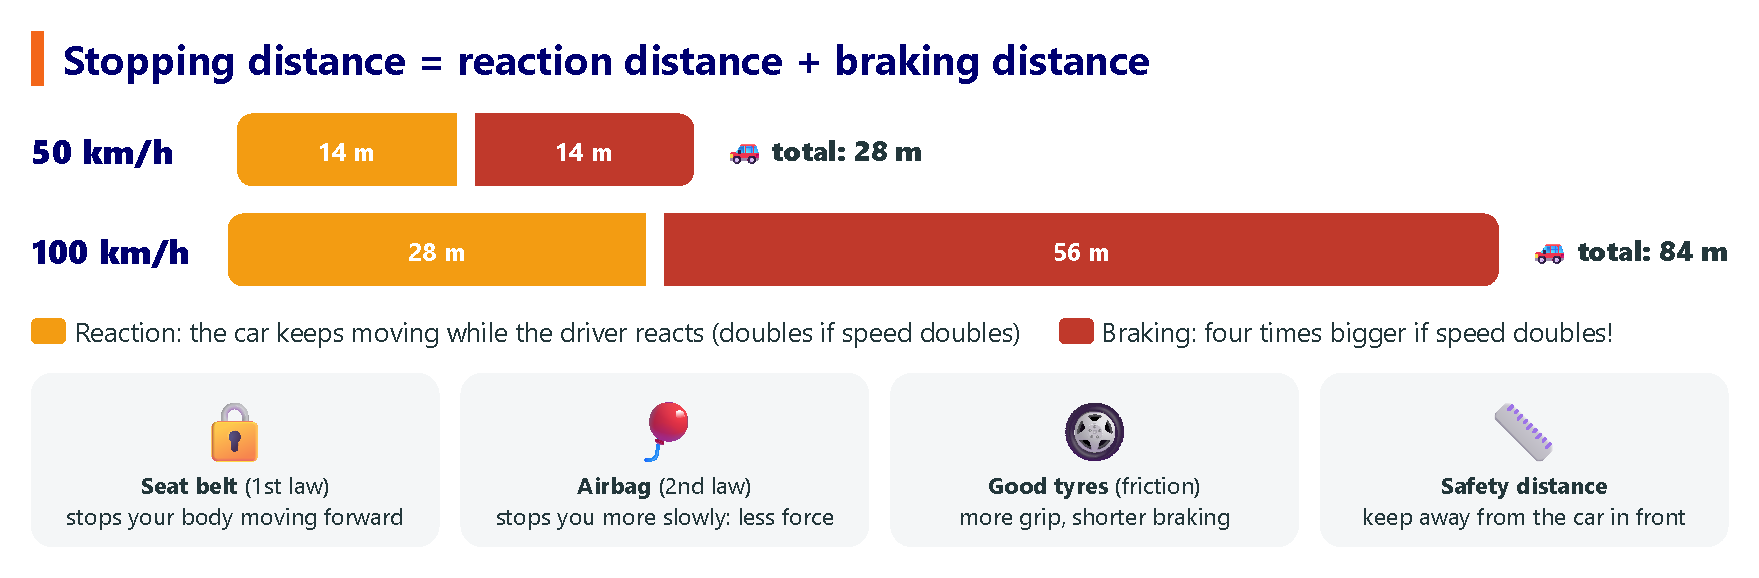
\includegraphics[width=\textwidth]{FigurasSVG/Unit_8_Forces/pdf/stopping_distance.pdf}
    \caption{Stopping distance at two speeds (approximate values). When the speed doubles, the reaction distance doubles, but the braking distance becomes four times larger, so the total stopping distance triples.}
    \label{fig:u8_stopping_distance}
\end{figure}

\begin{didyouknow}
    Wearing a seat belt roughly halves the risk of dying in a car crash. In a crash at only \qty{50}{\kmph}, an unbelted passenger hits the seat in front with a force similar to the weight of an elephant!
\end{didyouknow}

\begin{exercise}
    Explain, using Newton's first law (inertia), why passengers in a car must wear a seat belt even on short trips at low speed.
    \begin{solu}
        By the first law, a moving passenger's body tends to keep moving at the car's speed unless a force acts on it. If the car crashes and stops suddenly, without a seat belt the passenger's body would keep moving forward due to inertia and could hit the windscreen or the seat in front. The seat belt applies the force needed to decelerate the passenger together with the car, avoiding this.
    \end{solu}
\end{exercise}

\begin{exercise}
    A car of mass \qty{1200}{\kg} braking on a dry road can produce a maximum frictional (braking) force of \qty{6000}{\newton}.
    \begin{enumerate}[label=\letraminuscula]
        \item Calculate the maximum deceleration (in absolute value) that this braking force can produce.
        \item If the same road is wet and the maximum frictional force drops to \qty{3000}{\newton}, calculate the new maximum deceleration. Is the braking distance longer or shorter on the wet road, for the same initial speed?
    \end{enumerate}
    \begin{solu}
        \begin{enumerate}[label=\alph*)]
            \item \(a = \dfrac{F}{m} = \dfrac{\qty{6000}{\newton}}{\qty{1200}{\kg}} = \qty{5}{\mpss}\).
            \item \(a = \dfrac{\qty{3000}{\newton}}{\qty{1200}{\kg}} = \qty{2.5}{\mpss}\). \\
            Since the deceleration is smaller on the wet road, the car takes \textbf{longer, and travels a greater distance,} to stop from the same speed: \textbf{the braking distance is longer}.
        \end{enumerate}
    \end{solu}
\end{exercise}

\begin{exercise}
    A cyclist travelling at \qty{10}{\mps} takes \qty{0.5}{\s} to react before braking (during this time she keeps moving at constant speed). Once she brakes, she decelerates uniformly at \qty{4}{\mpss} until she stops.
    \begin{enumerate}[label=\letraminuscula]
        \item Calculate the distance travelled during the reaction time.
        \item Calculate how long it takes her to stop once she starts braking, and the braking distance (using the triangle formula for the area under the speed-time graph).
        \item Calculate the total stopping distance (reaction distance \(+\) braking distance).
    \end{enumerate}
    \begin{solu}
        \begin{enumerate}[label=\alph*)]
            \item Reaction distance \(= v \cdot t_{\text{reaction}} = \qty{10}{\mps} \cdot \qty{0.5}{\s} = \qty{5}{\m}\).
            \item Time to stop: \(t = \dfrac{v_{\text{final}} - v_{\text{initial}}}{a} = \dfrac{0 - \qty{10}{\mps}}{\qty{-4}{\mpss}} = \qty{2.5}{\s}\). \\
            Braking distance \(= \dfrac{v_{\text{initial}} \cdot t}{2} = \dfrac{\qty{10}{\mps} \cdot \qty{2.5}{\s}}{2} = \qty{12.5}{\m}\).
            \item Total stopping distance \(= \qty{5}{\m} + \qty{12.5}{\m} = \qty{17.5}{\m}\): this is the minimum safety distance she should keep from the vehicle in front.
        \end{enumerate}
    \end{solu}
\end{exercise}

%----------------------------------------------------------------------------------------

\section{Forces and deformation}

When a deforming force is applied, objects can behave in different ways:

\begin{figure}[H]
    \centering
    % [FIGURA ORIGINAL] \includegraphics[width=\textwidth]{Unit_8/deformation}
    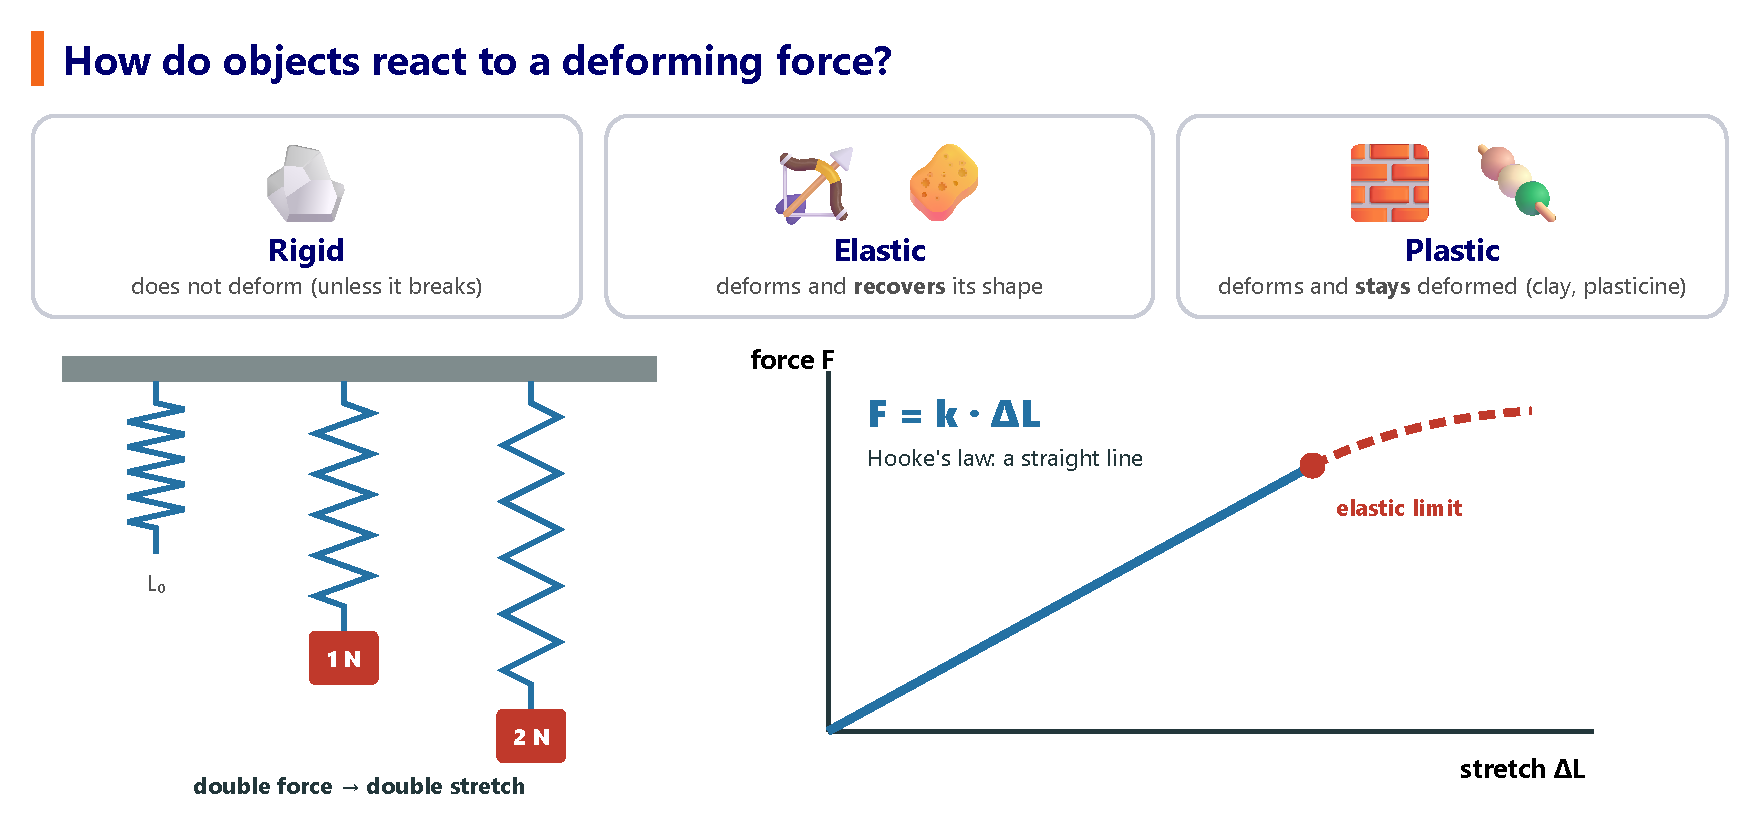
\includegraphics[width=\textwidth]{FigurasSVG/Unit_8_Forces/pdf/deformation.pdf}
    \caption{Rigid, elastic and plastic objects, and Hooke's law for a spring.}
    \label{fig:u8_deformation}
\end{figure}

\begin{impt}
    A very strong deforming force can make a rigid body exceed its \negsubro{breaking point} and break, or make an elastic body exceed its \negsubro{elastic limit} and become permanently deformed.
\end{impt}

Forces are measured with a \negsubro{dynamometer}: a calibrated spring that stretches, or compresses, in proportion to the force applied.

\begin{definition}[Hooke's law]
    The deformation (stretch) of a spring, \(\Delta L\), is directly proportional to the force applied:
    \begin{equation*}
        F = k \cdot \Delta L
    \end{equation*}
    where \(k\) is the \textbf{constant of elasticity}, a characteristic property of the spring, measured in \unit{\newton\per\metre}.
\end{definition}

\begin{example}
    \textbf{A spring \qty{20}{\cm} long is stretched to \qty{23}{\cm} when pulled with a force of \qty{1.5}{\newton}. Calculate:}
    \begin{enumerate}[label=\letraminuscula]
        \item Its constant of elasticity.
        \item Its length when pulled with a force of \qty{5}{\newton}.
    \end{enumerate}
    \begin{enumerate}[label=\alph*)]
        \item \(\Delta L = \qty{23}{\cm} - \qty{20}{\cm} = \qty{3}{\cm} = \qty{0.03}{\m}\). \\
        \(k = \dfrac{F}{\Delta L} = \dfrac{\qty{1.5}{\newton}}{\qty{0.03}{\m}} = \qty{50}{\newton\per\metre}\).
        \item \(\Delta L = \dfrac{F}{k} = \dfrac{\qty{5}{\newton}}{\qty{50}{\newton\per\metre}} = \qty{0.1}{\m} = \qty{10}{\cm}\). \\
        \(L = L_0 + \Delta L = \qty{20}{\cm} + \qty{10}{\cm} = \qty{30}{\cm}\).
    \end{enumerate}
\end{example}

\begin{exercise}
    A spring that is \qty{20}{\cm} long has a constant of elasticity of \qty{100}{\newton\per\metre}. Calculate the force needed to pull it so that it stretches to \qty{23}{\cm}.
    \begin{solu}
        \(\Delta L = \qty{23}{\cm} - \qty{20}{\cm} = \qty{0.03}{\m}\). \\
        \(F = k \cdot \Delta L = \qty{100}{\newton\per\metre} \cdot \qty{0.03}{\m} = \qty{3}{\newton}\).
    \end{solu}
\end{exercise}

\begin{exercise}
    The spring of a kitchen scale is \qty{5}{\cm} long and has a constant of elasticity of \qty{800}{\newton\per\metre}. An object weighing \qty{8}{\newton} is placed on the scale.
    \begin{enumerate}[label=\letraminuscula]
        \item How long is the spring now?
    \end{enumerate}
    \begin{solu}
        \(\Delta L = \dfrac{F}{k} = \dfrac{\qty{8}{\newton}}{\qty{800}{\newton\per\metre}} = \qty{0.01}{\m} = \qty{1}{\cm}\). \\
        \(L = L_0 + \Delta L = \qty{5}{\cm} + \qty{1}{\cm} = \qty{6}{\cm}\).
    \end{solu}
\end{exercise}

\begin{exercise}
    Two springs, \(A\) and \(B\), are stretched with the same force of \qty{4}{\newton}. Spring \(A\) stretches \qty{2}{\cm} and spring \(B\) stretches \qty{5}{\cm}.
    \begin{enumerate}[label=\letraminuscula]
        \item Calculate the constant of elasticity of each spring.
        \item Which spring is ``stiffer'' (harder to stretch)? Justify your answer using the value of \(k\).
    \end{enumerate}
    \begin{solu}
        \begin{enumerate}[label=\alph*)]
            \item \(k_A = \dfrac{F}{\Delta L} = \dfrac{\qty{4}{\newton}}{\qty{0.02}{\m}} = \qty{200}{\newton\per\metre}\). \\
            \(k_B = \dfrac{F}{\Delta L} = \dfrac{\qty{4}{\newton}}{\qty{0.05}{\m}} = \qty{80}{\newton\per\metre}\).
            \item Spring \(A\) is stiffer, because it has a \textbf{larger} constant of elasticity: for the same force, it stretches less, so more force is needed to produce a given deformation.
        \end{enumerate}
    \end{solu}
\end{exercise}

\begin{exercise}
    A spring has a natural length of \qty{15}{\cm}. When a force of \qty{6}{\newton} is applied, it stretches to \qty{21}{\cm}.
    \begin{enumerate}[label=\letraminuscula]
        \item Calculate its constant of elasticity.
        \item The spring's elastic limit corresponds to a maximum stretch of \qty{10}{\cm}. What is the maximum force it can support while still behaving elastically?
    \end{enumerate}
    \begin{solu}
        \begin{enumerate}[label=\alph*)]
            \item \(\Delta L = \qty{21}{\cm} - \qty{15}{\cm} = \qty{6}{\cm} = \qty{0.06}{\m}\). \\
            \(k = \dfrac{F}{\Delta L} = \dfrac{\qty{6}{\newton}}{\qty{0.06}{\m}} = \qty{100}{\newton\per\metre}\).
            \item \(F_{\text{max}} = k \cdot \Delta L_{\text{max}} = \qty{100}{\newton\per\metre} \cdot \qty{0.10}{\m} = \qty{10}{\newton}\).
        \end{enumerate}
    \end{solu}
\end{exercise}

%----------------------------------------------------------------------------------------

%----------------------------------------------------------------------------------------

\section*{Summary}

\begin{itemize}
    \item \textbf{Newton's laws}: 1st (inertia, no net force \(\to\) no change in motion); 2nd (\(F = m \cdot a\)); 3rd (action-reaction, on different objects).
    \item \textbf{Weight vs.\ mass}: mass (\(m\), kg) does not change; weight (\(W = m \cdot g\), N) is a force and changes with \(g\).
    \item \textbf{Friction} opposes relative motion between surfaces; it is essential in road safety, together with seat belts, airbags and adequate braking/safety distances (applications of Newton's laws).
    \item \textbf{Deformation}: rigid (no deformation), elastic (returns to shape), plastic (stays deformed). \textbf{Hooke's law}: \(F = k \cdot \Delta L\).
\end{itemize}

\section{Vocabulary}

\begin{vocabulary}[Inertia]
    The tendency of an object to keep its state of motion (rest or URM) unless a net force acts on it. \newline
    \textbf{Translation to Spanish}: Inercia
\end{vocabulary}

\begin{vocabulary}[Net force]
    The overall force acting on an object, obtained by adding all the individual forces acting on it. \newline
    \textbf{Translation to Spanish}: Fuerza neta / resultante
\end{vocabulary}

\begin{vocabulary}[Dynamometer]
    An instrument used to measure forces, based on a calibrated spring. \newline
    \textbf{Translation to Spanish}: Dinamómetro
\end{vocabulary}

\begin{vocabulary}[Elastic limit]
    The maximum deformation an elastic body can undergo and still return to its original shape. \newline
    \textbf{Translation to Spanish}: Límite de elasticidad
\end{vocabulary}

\begin{vocabulary}[Weight]
    The force with which a celestial body attracts a mass towards its centre; \(W = m \cdot g\). \newline
    \textbf{Translation to Spanish}: Peso
\end{vocabulary}

\begin{vocabulary}[Mass]
    The amount of matter in a body; it does not change from place to place. \newline
    \textbf{Translation to Spanish}: Masa
\end{vocabulary}

\begin{vocabulary}[Friction force]
    A force that opposes the relative motion between two surfaces in contact. \newline
    \textbf{Translation to Spanish}: Fuerza de rozamiento
\end{vocabulary}

\begin{vocabulary}[Braking distance]
    The distance a vehicle travels between the moment the brakes are applied and the moment it stops. \newline
    \textbf{Translation to Spanish}: Distancia de frenado
\end{vocabulary}



%------------------------------------------------


    \chapterimage{images/portada_cabeceras/cabecera_Unit9}
    \chapter{Energy}
    % Saberes básicos (LOMLOE) asociados a esta unidad
%
% Bloque A. Las destrezas científicas básicas
%   - Uso del lenguaje científico y de las unidades del Sistema Internacional (SI):
%     la unidad se trabaja con el julio y sus múltiplos/submúltiplos, además de otras
%     unidades de energía de uso habitual (caloría, kWh, tep), reforzando el manejo
%     correcto de magnitudes y unidades ya introducido en la Unidad 1.
%
% Bloque C. La energía
%   - Formulación de cuestiones e hipótesis sobre la energía, sus propiedades y
%     manifestaciones como causa de todos los procesos de cambio: se define la energía,
%     sus formas (cinética, potencial, térmica, eléctrica, radiante, química, nuclear)
%     y sus propiedades (se transfiere, se almacena, se transporta, se transforma,
%     se degrada y se conserva).
%   - Diseño y comprobación experimental de hipótesis sobre el uso doméstico e industrial
%     de la energía y las transformaciones entre sus distintas formas: se analizan cadenas
%     de transformación energética en aparatos cotidianos (linterna, secador, aerogenerador,
%     hervidor, panel solar) y el concepto de degradación/rendimiento.
%   - Elaboración fundamentada de hipótesis sobre el medio ambiente y la sostenibilidad a
%     partir de las diferencias entre fuentes renovables y no renovables. Valoración de la
%     producción de energía eólica en Castilla-La Mancha: se dedica un apartado específico
%     a la energía eólica en la región, con sus ventajas y sus impactos.
%   - Efectos del calor sobre la materia: se incorpora un apartado sobre el calor específico
%     y la dilatación térmica, con ejemplos y aplicaciones cotidianas (juntas de dilatación,
%     termómetros de líquido, clima costero frente a clima de interior).
%   - Naturaleza eléctrica de la materia: electrización de los cuerpos, circuitos eléctricos
%     y obtención de energía eléctrica: se desarrollan la ley de Ohm y los circuitos en serie
%     y en paralelo, junto con el ahorro energético y la conservación sostenible del medio
%     ambiente, ya tratados en la unidad.

\spacing{1.3}
\raggedbottom % pages with large figures end where the text ends (no stretched gaps between boxes)

\section{What is energy?}

\begin{definition}[Energy]
    A physical quantity that measures the capacity of a body to produce changes in itself or in other bodies.
\end{definition}

Whenever a person, a machine or any other object does something, it uses energy and has to get more in order to keep working.

\begin{didyouknow}
    Your brain uses about 20\,\% of all the energy your body gets from food, even though it is only about 2\,\% of your body mass!
\end{didyouknow}

\subsection{How is energy measured?}

In the SI, energy is measured in \textbf{joules} (J); the kilojoule (\qty{1}{\kj} = \qty{1000}{\joule}) is also common. There are also other units, used in specific fields:

\begin{itemize}
    \item \negsubro{Calorie} (cal): the amount of heat needed to raise the temperature of \qty{1}{\g} of water by \qty{1}{\celsius}. \(\qty{1}{\calorie} = \qty{4.18}{\joule}\). Food energy is traditionally given in Calories (with a capital C): \(1 \text{ Calorie} = 1000 \text{ calories} = \qty{1}{\kilo\calorie}\).
    \item \negsubro{Kilowatt-hour} (kWh): used to measure electrical energy; it is the energy consumed by a \qty{1}{\kW} appliance used for one hour. \(\qty{1}{\kwh} = \qty{3.6e6}{\joule}\).
    \item \negsubro{Tonne of oil equivalent} (toe): used in the oil industry; it is the energy obtained by burning \qty{1000}{\kg} of petroleum. \(1 \text{ toe} \approx \qty{4.187e10}{\joule}\).
\end{itemize}

\begin{figure}[H]
    \centering
    % [FIGURA ORIGINAL] \includegraphics[width=\textwidth]{Unit_9/energy_units}
    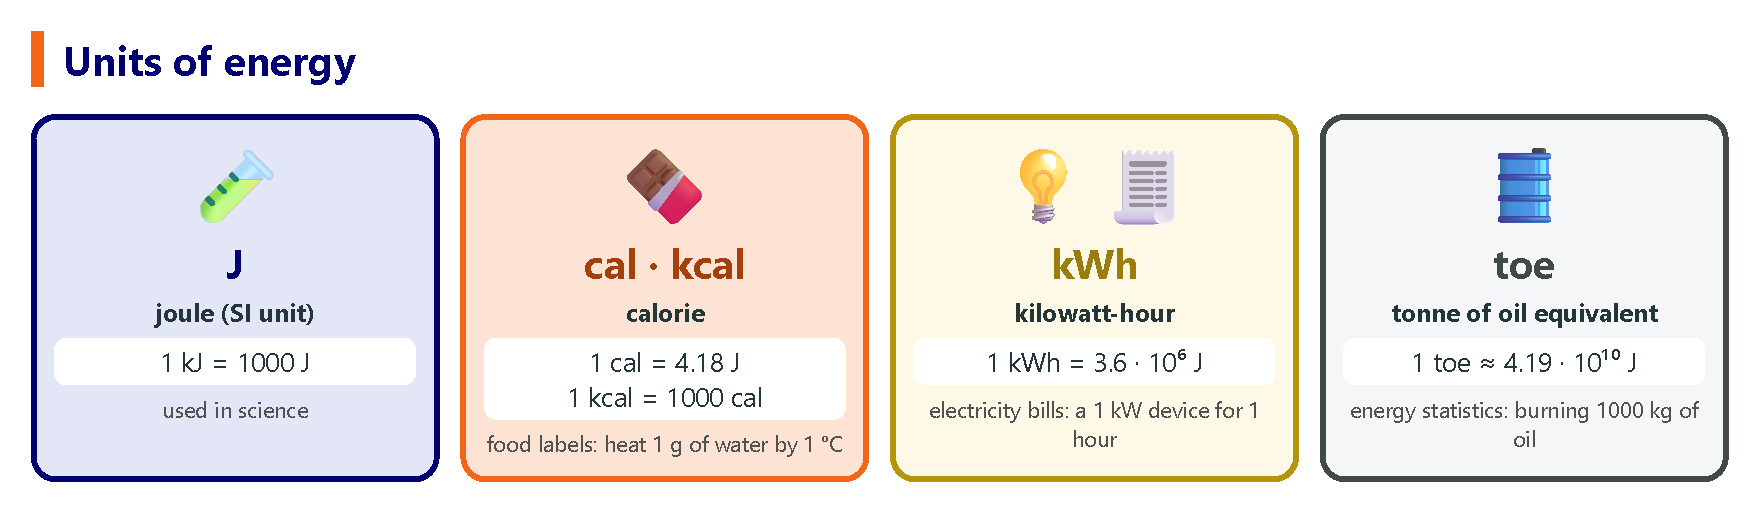
\includegraphics[width=\textwidth]{FigurasSVG/Unit_9_Energy/pdf/energy_units.pdf}
    \caption{The most common units of energy and where we find them.}
    \label{fig:u9_energy_units}
\end{figure}

\begin{example}
    \textbf{A ball falls from a basket to the floor with an energy of \qty{18.2}{\joule}. Write this amount in kJ, cal and kWh.}
    \begin{align*}
        \qty{18.2}{\joule} \cdot \dfrac{\qty{1}{\kilo\joule}}{\qty{1000}{\joule}} &= \textbf{0.018 kJ} \\
        \qty{18.2}{\joule} \cdot \dfrac{\qty{1}{\calorie}}{\qty{4.18}{\joule}} &= \textbf{4.35 cal} \\
        \qty{18.2}{\joule} \cdot \dfrac{\qty{1}{\kwh}}{\qty{3.6e6}{\joule}} &\approx \textbf{5.06} \times \textbf{10}^{\textbf{-6}} \textbf{ kWh}
    \end{align*}
\end{example}

\begin{exercise}
    To make a cup of tea, water is heated from \qty{20}{\celsius} to \qty{100}{\celsius} in a microwave that supplies \qty{83860}{\joule}.
    \begin{enumerate}[label=\letraminuscula]
        \item How many calories is this?
        \item How many kWh is it?
    \end{enumerate}
    \begin{solu}
        \begin{enumerate}[label=\alph*)]
            \item \(\qty{83860}{\joule} \cdot \dfrac{\qty{1}{\calorie}}{\qty{4.18}{\joule}} \approx 20062\) cal.
            \item \(\qty{83860}{\joule} \cdot \dfrac{\qty{1}{\kwh}}{\qty{3.6e6}{\joule}} \approx 0.0233\) kWh.
        \end{enumerate}
    \end{solu}
\end{exercise}

\begin{exercise}
    The energy content of \qty{100}{\g} of biscuits is approximately \qty{350}{\kilo\calorie}. Write this amount in joules.
    \begin{solu}
        \(\qty{350}{\kilo\calorie} = \qty{350000}{\calorie}\); \(\qty{350000}{\calorie} \cdot \qty{4.18}{\joule\per\calorie} \approx \qty{1463000}{\joule} \approx \qty{1.46}{\mega\joule}\).
    \end{solu}
\end{exercise}

\begin{exercise}
    A washing machine uses \qty{1.1}{\kwh} of electrical energy to complete a wash cycle.
    \begin{enumerate}[label=\letraminuscula]
        \item Convert this energy into joules.
        \item Convert this energy into calories.
    \end{enumerate}
    \begin{solu}
        \begin{enumerate}[label=\alph*)]
            \item \(\qty{1.1}{\kwh} \cdot \qty{3.6e6}{\joule\per\kwh} = \qty{3960000}{\joule} \approx \qty{3.96}{\mega\joule}\).
            \item \(\qty{3960000}{\joule} \cdot \dfrac{\qty{1}{\calorie}}{\qty{4.18}{\joule}} \approx 947368\) cal \(\approx 947.4\) kcal.
        \end{enumerate}
    \end{solu}
\end{exercise}

\begin{exercise}
    A solar panel installation produces \qty{2.5}{\mega\joule} of energy in a day. Express this amount in kWh and in kcal.
    \begin{solu}
        \(\qty{2.5}{\mega\joule} = \qty{2500000}{\joule}\). \\
        In kWh: \(\qty{2500000}{\joule} \cdot \dfrac{\qty{1}{\kwh}}{\qty{3.6e6}{\joule}} \approx \textbf{0.694 kWh}\). \\
        In kcal: \(\qty{2500000}{\joule} \cdot \dfrac{\qty{1}{\calorie}}{\qty{4.18}{\joule}} \approx 598086\) cal \(\approx \textbf{598.1 kcal}\).
    \end{solu}
\end{exercise}

%----------------------------------------------------------------------------------------

\section{Forms of energy}

\begin{figure}[H]
    \centering
    % [FIGURA ORIGINAL] \includegraphics[width=\textwidth]{Unit_9/forms_energy}
    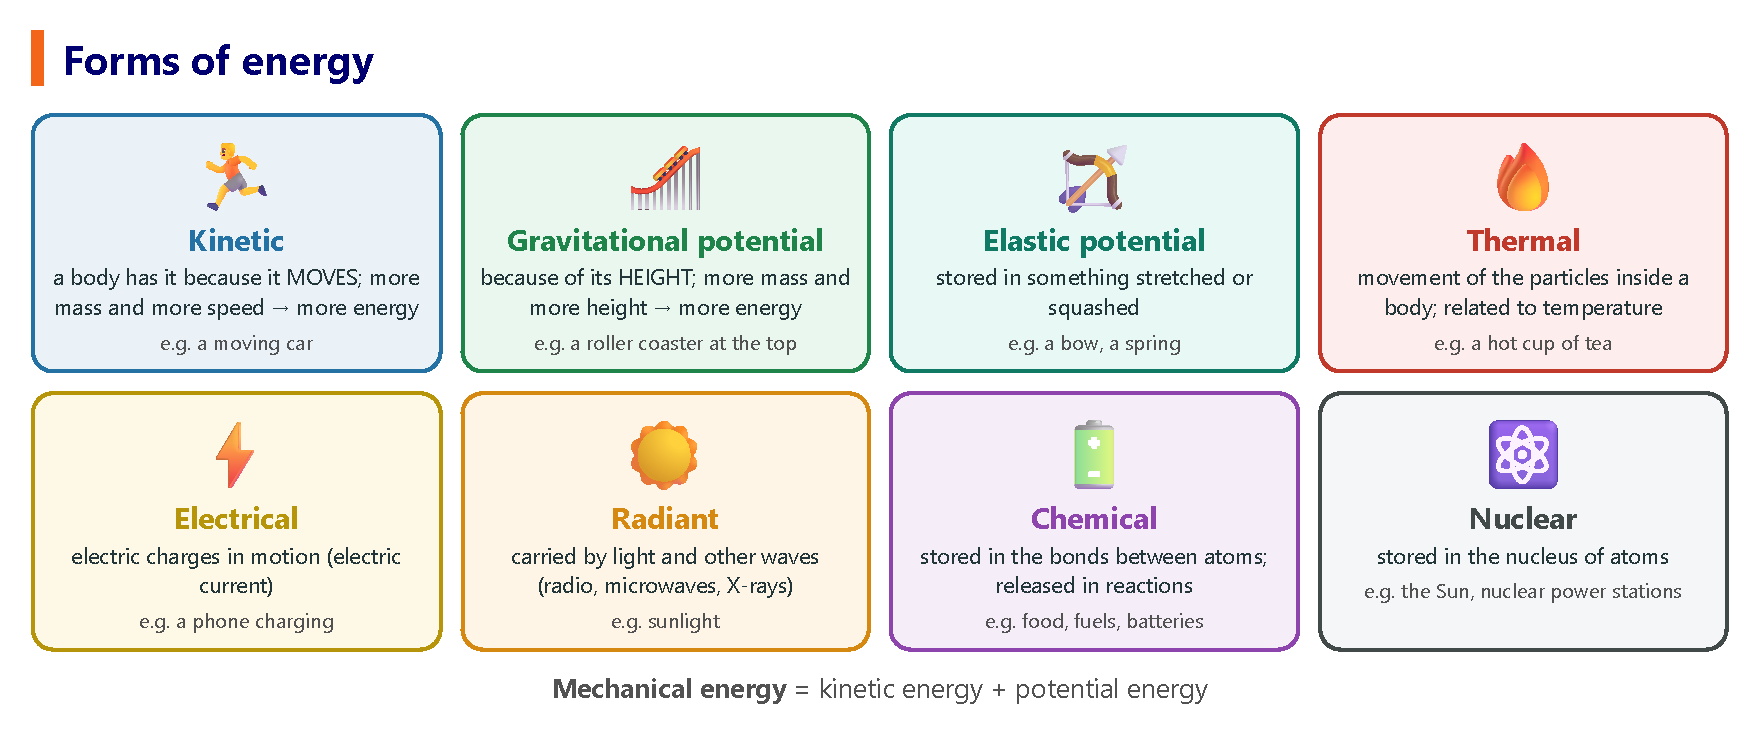
\includegraphics[width=\textwidth]{FigurasSVG/Unit_9_Energy/pdf/forms_energy.pdf}
    \caption{The forms of energy.}
    \label{fig:u9_forms_energy}
\end{figure}

\begin{impt}
    \negsubro{Nuclear fusion vs.\ nuclear fission}:
    \begin{itemize}
        \item \textbf{Nuclear fusion}: light atoms join together to form larger atoms, releasing energy (this happens in the Sun and other stars).
        \item \textbf{Nuclear fission}: heavy atoms break apart into smaller atoms, releasing energy (this happens in nuclear power stations).
    \end{itemize}
\end{impt}

\begin{figure}[H]
    \centering
    % [FIGURA ORIGINAL] \includegraphics[width=\textwidth]{Unit_9/fusion_fission}
    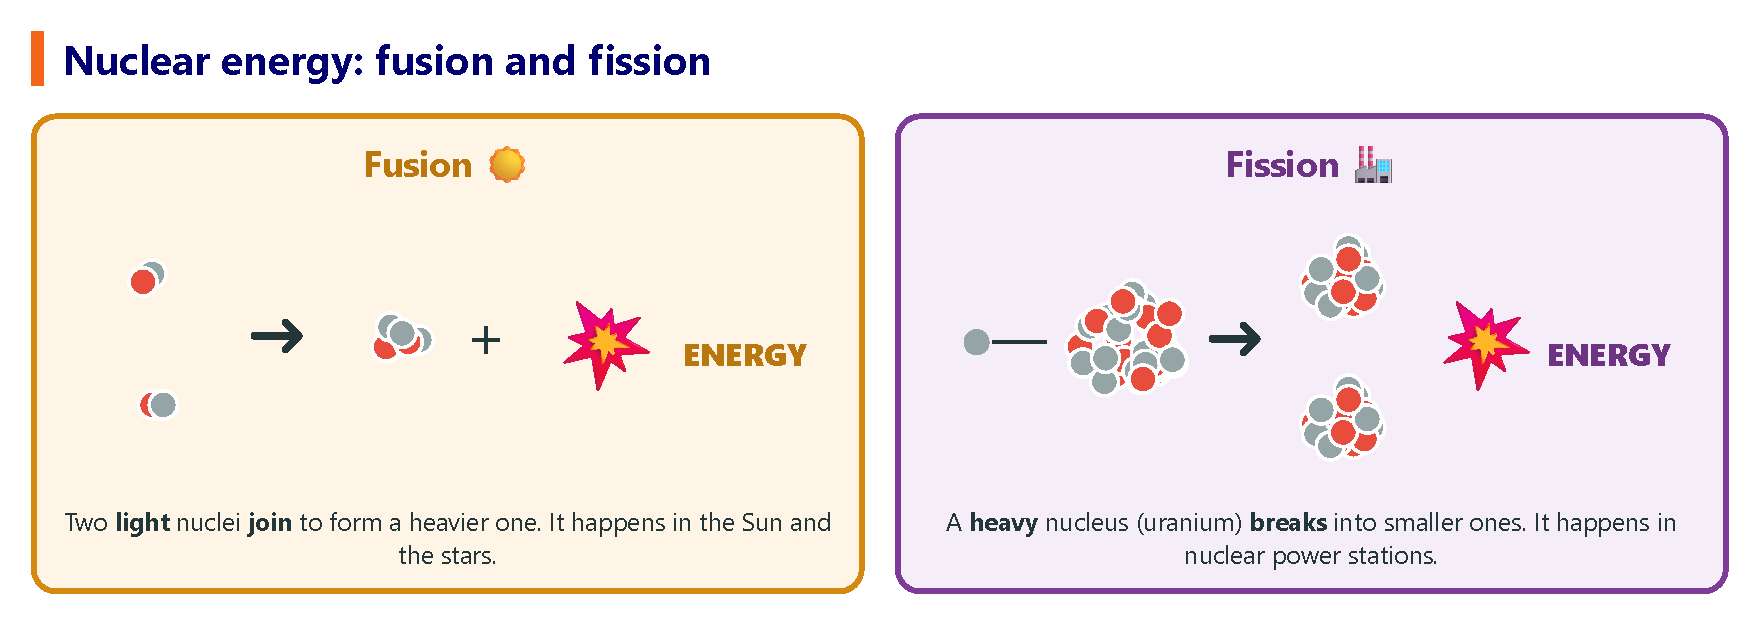
\includegraphics[width=\textwidth]{FigurasSVG/Unit_9_Energy/pdf/fusion_fission.pdf}
    \caption{Nuclear fusion and nuclear fission.}
    \label{fig:u9_fusion_fission}
\end{figure}

\begin{didyouknow}
    Every second, the Sun turns about 4 million tonnes of matter into energy by nuclear fusion. It has been doing this for 4\,600 million years, and it still has fuel for about 5\,000 million years more!
\end{didyouknow}

\begin{example}
    A lorry and a car travel at the same speed; the lorry has more \textbf{kinetic energy} because it has more mass. The same car has more kinetic energy when it travels faster. A ball has more \textbf{gravitational potential energy} the higher it is and the more mass it has. A stretched bow has more \textbf{elastic potential energy} the more it is stretched.
\end{example}

\begin{exercise}
    Say which form(s) of energy is/are involved in each situation: a) a moving bicycle; b) a hairdryer heating and blowing air; c) a swimmer diving into a pool; d) a hot cup of tea; e) an X-ray image; f) a stretched slingshot.
    \begin{solu}
        \begin{enumerate}[label=\alph*)]
            \item Kinetic (mechanical) energy.
            \item Electrical energy (transformed into thermal and kinetic energy of the air).
            \item Kinetic and gravitational potential energy.
            \item Thermal energy.
            \item Radiant energy.
            \item Elastic potential energy.
        \end{enumerate}
    \end{solu}
\end{exercise}

\begin{exercise}
    What types of energy are involved when a mobile phone is being used, and what transformations take place?
    \begin{solu}
        The battery stores \textbf{chemical energy}; when the phone is used, this is transformed into \textbf{electrical energy}, which the phone transforms into \textbf{radiant energy} (screen light), \textbf{thermal energy} (the phone warming up) and, if used for a call, \textbf{sound-related} (mechanical) energy in the loudspeaker.
    \end{solu}
\end{exercise}

\begin{exercise}
    Classify the main energy transformation involved in each case (before \(\to\) after): a) a solar cooker; b) a wound-up clockwork toy car; c) a lit match; d) a nuclear power station.
    \begin{solu}
        \begin{enumerate}[label=\alph*)]
            \item Radiant energy (sunlight) \(\to\) thermal energy.
            \item Elastic potential energy (wound spring) \(\to\) kinetic energy.
            \item Chemical energy \(\to\) thermal energy \(+\) radiant energy (light).
            \item Nuclear energy \(\to\) thermal energy \(\to\) electrical energy.
        \end{enumerate}
    \end{solu}
\end{exercise}

%----------------------------------------------------------------------------------------

\section{Properties of energy}

\begin{figure}[H]
    \centering
    % [FIGURA ORIGINAL] \includegraphics[width=\textwidth]{Unit_9/energy_properties}
    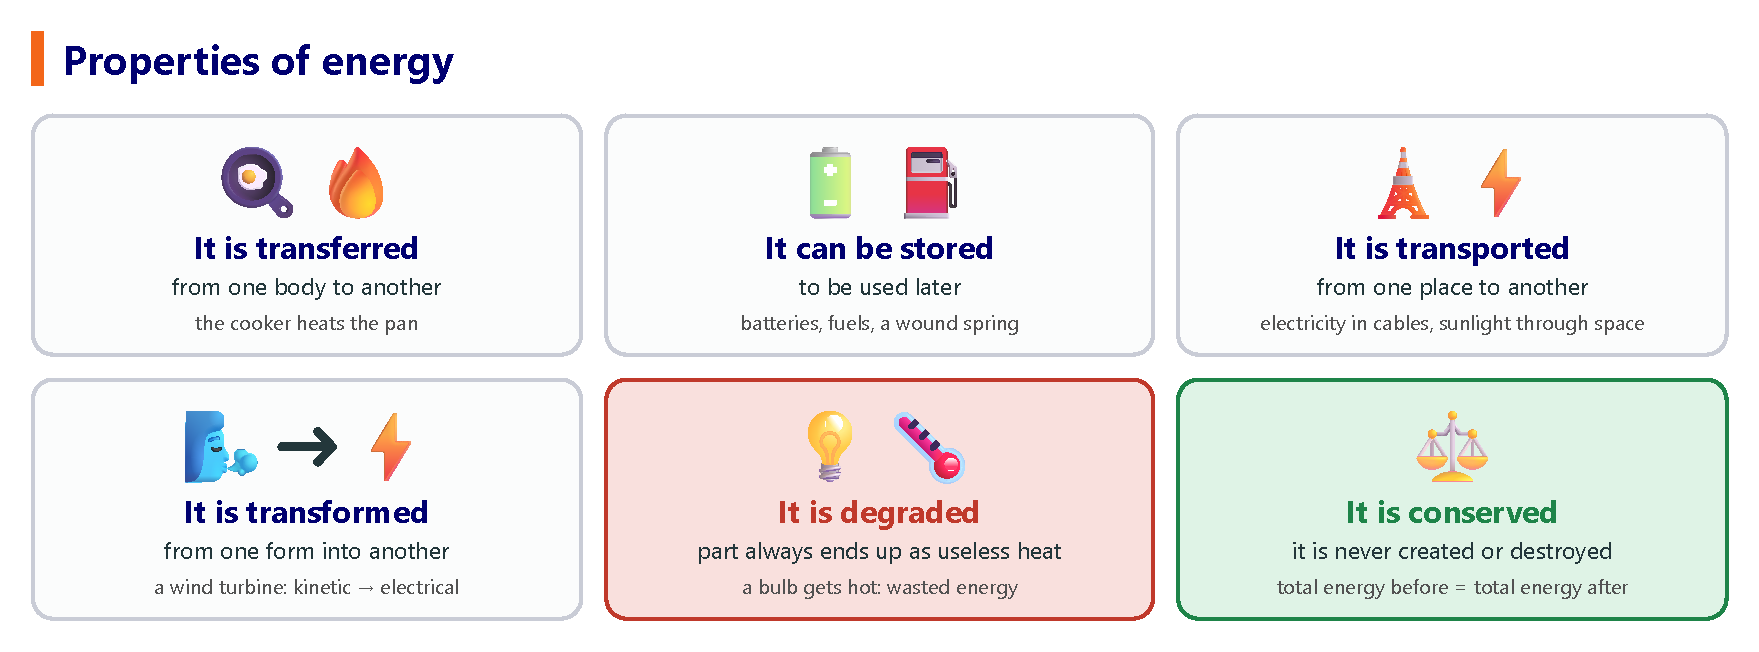
\includegraphics[width=\textwidth]{FigurasSVG/Unit_9_Energy/pdf/energy_properties.pdf}
    \caption{The six properties of energy.}
    \label{fig:u9_energy_properties}
\end{figure}

\begin{example}
    \textbf{Energy transformation chain in an electric torch (flashlight)}: chemical energy (battery) \(\to\) electrical energy \(\to\) radiant energy (light) \(+\) thermal energy (degraded, warms the torch). The total energy transformed is conserved, but only the radiant energy is useful.
\end{example}

\begin{figure}[H]
    \centering
    % [FIGURA ORIGINAL] \includegraphics[width=\textwidth]{Unit_9/torch_chain}
    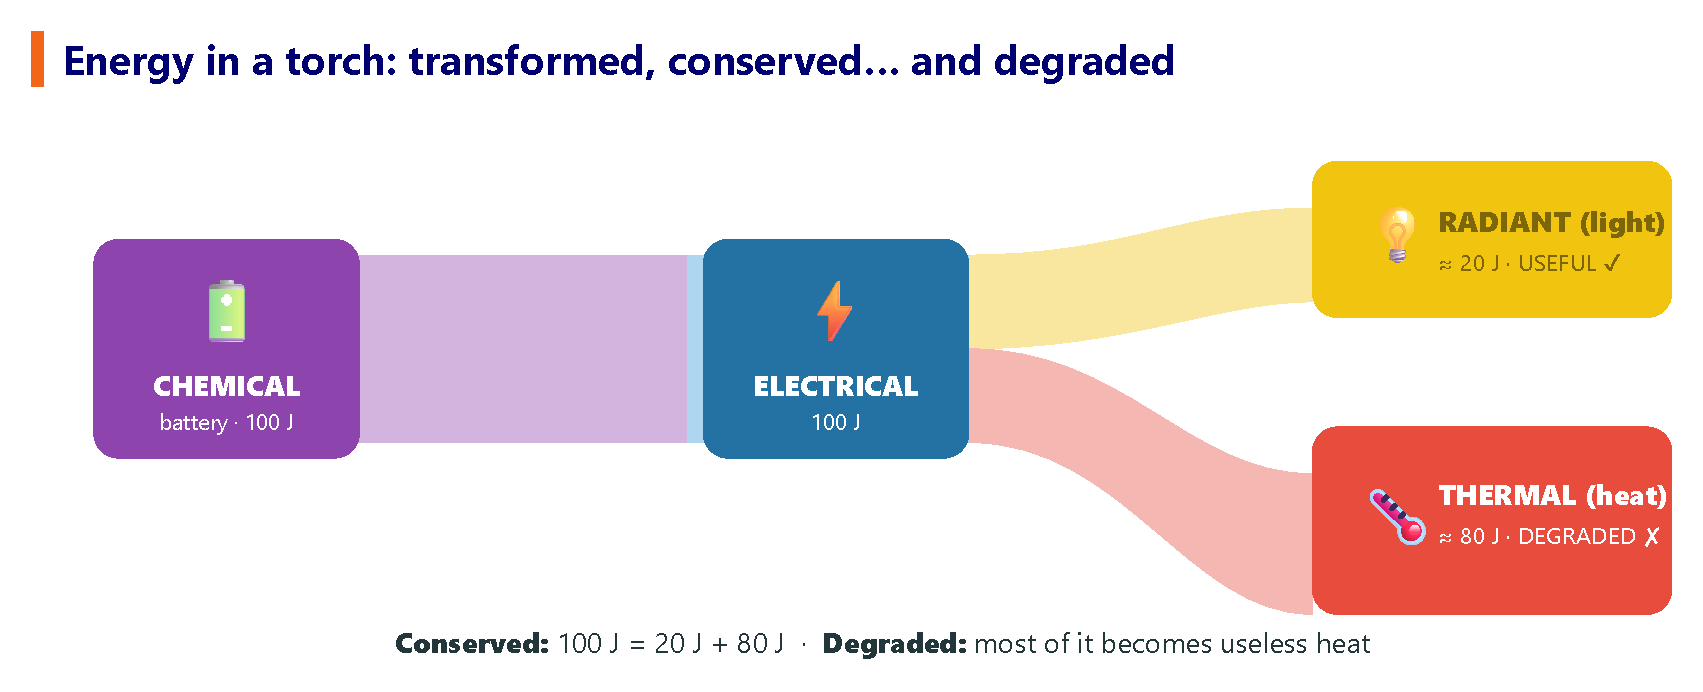
\includegraphics[width=\textwidth]{FigurasSVG/Unit_9_Energy/pdf/torch_chain.pdf}
    \caption{Energy in a torch: the total energy is conserved, but most of it is degraded into heat.}
    \label{fig:u9_torch_chain}
\end{figure}

\begin{exercise}
    For each device, write the chain of energy transformations from the energy source to the useful energy obtained: a) a wind turbine generating electricity; b) an electric kettle boiling water; c) a solar panel that heats water directly (no electricity involved).
    \begin{solu}
        \begin{enumerate}[label=\alph*)]
            \item Kinetic energy (wind) \(\to\) mechanical energy (rotating blades and generator) \(\to\) electrical energy.
            \item Electrical energy \(\to\) thermal energy (heats the water).
            \item Radiant energy (sunlight) \(\to\) thermal energy (heats the water directly).
        \end{enumerate}
    \end{solu}
\end{exercise}

\begin{exercise}
    A ball is dropped from a height and bounces several times, each time reaching a lower height than the previous one. Using the properties of energy, explain why this happens, and say whether any energy is destroyed.
    \begin{solu}
        At each bounce, part of the ball's mechanical energy is \textbf{transformed} into thermal energy and sound due to friction with the air and deformation on impact; this is energy \textbf{degradation}, so less useful (mechanical) energy is available for the next bounce, and it reaches a lower height each time. No energy is destroyed: the total energy is always \textbf{conserved}, it is just transformed into less useful forms.
    \end{solu}
\end{exercise}

\subsection{How bodies exchange energy}

\begin{itemize}
    \item \negsubro{In the form of heat}: bodies at different temperatures exchange energy until they reach the same temperature (e.g.\ ice melting absorbs heat from the air).
    \item \negsubro{In the form of mechanical work}: happens when a force causes a movement (e.g.\ pulling back a bow, pushing a shopping trolley).
\end{itemize}

\begin{figure}[H]
    \centering
    % [FIGURA ORIGINAL] \includegraphics[width=\textwidth]{Unit_9/heat_work}
    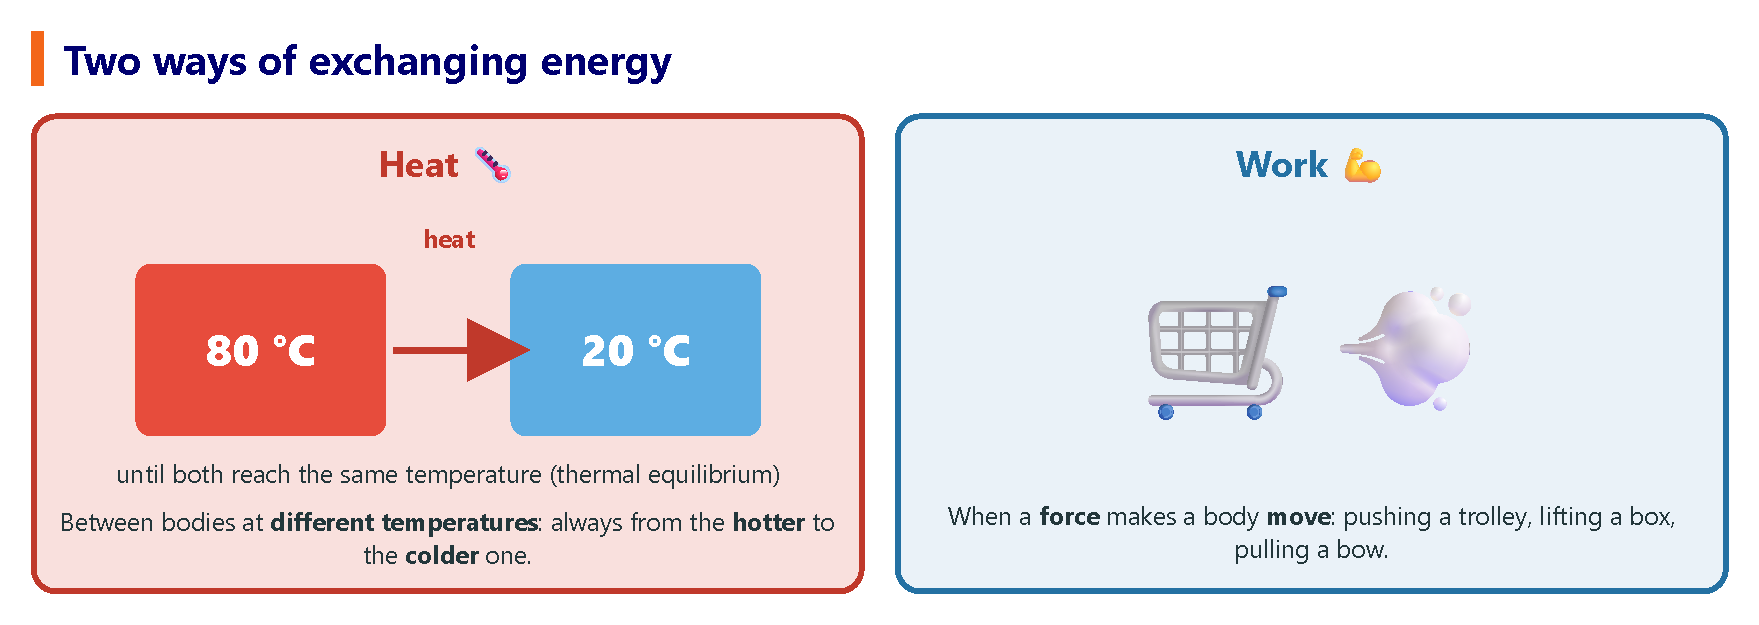
\includegraphics[width=\textwidth]{FigurasSVG/Unit_9_Energy/pdf/heat_work.pdf}
    \caption{Bodies exchange energy as heat or as work.}
    \label{fig:u9_heat_work}
\end{figure}

\begin{exercise}
    Identify the energy property involved in each situation: a) when we plug in a hairdryer, a current of air appears; b) a mobile phone battery lasts three days; c) when we put a bottle of water in the fridge, it cools down; d) light bulbs that heat up are not very efficient; e) high-voltage cables carry electricity across the country.
    \begin{solu}
        \begin{enumerate}[label=\alph*)]
            \item Energy is \textbf{transformed} (electrical into kinetic and thermal).
            \item Energy is \textbf{stored} (chemical energy in the battery).
            \item Energy is \textbf{transferred} in the form of heat (from the water to the cold air in the fridge).
            \item Energy is \textbf{degraded} (part of the electrical energy becomes heat instead of light).
            \item Energy is \textbf{transported}.
        \end{enumerate}
    \end{solu}
\end{exercise}

\begin{exercise}
    The efficiency of a machine is the relationship between the energy we want to obtain from it and the energy it consumes. Which property of energy always makes the efficiency of a machine lower than 100\,\%?
    \begin{solu}
        \textbf{Energy degradation}: every time energy is transformed, part of it is converted into non-useful heat, so a machine can never return 100\,\% of the energy it consumes as useful energy.
    \end{solu}
\end{exercise}

\begin{exercise}
    Two metal blocks, one at \qty{80}{\celsius} and the other at \qty{20}{\celsius}, are placed in contact inside an insulated box. Describe what happens to the energy of each block until they reach thermal equilibrium, and name the form in which the energy is exchanged.
    \begin{solu}
        Heat flows from the hotter block (\qty{80}{\celsius}) to the colder one (\qty{20}{\celsius}) until both reach the same intermediate temperature (thermal equilibrium). The energy is exchanged \textbf{in the form of heat}; no mechanical work is done, since neither block moves.
    \end{solu}
\end{exercise}

\subsection{Effects of heat on matter}

\begin{definition}[Specific heat capacity]
    The amount of heat needed to raise the temperature of \qty{1}{\kg} of a substance by \qty{1}{\celsius}. Its symbol is \(c\), and its SI unit is \unit{\joule\per\kg\per\celsius}.
    \begin{equation*}
        Q = m \cdot c \cdot \Delta T
    \end{equation*}
\end{definition}

Water has a very high specific heat, \(c_{\text{water}} = \qty{4180}{\joule\per\kg\per\celsius}\) (equivalent to \(\qty{1}{\calorie}/(\text{g} \cdot {}^{\circ}\text{C})\)): this is why water heats up and cools down more slowly than most other substances, and why places near the coast tend to have milder climates than places far from the sea.

\begin{figure}[H]
    \centering
    % [FIGURA ORIGINAL] \includegraphics[width=\textwidth]{Unit_9/specific_heat}
    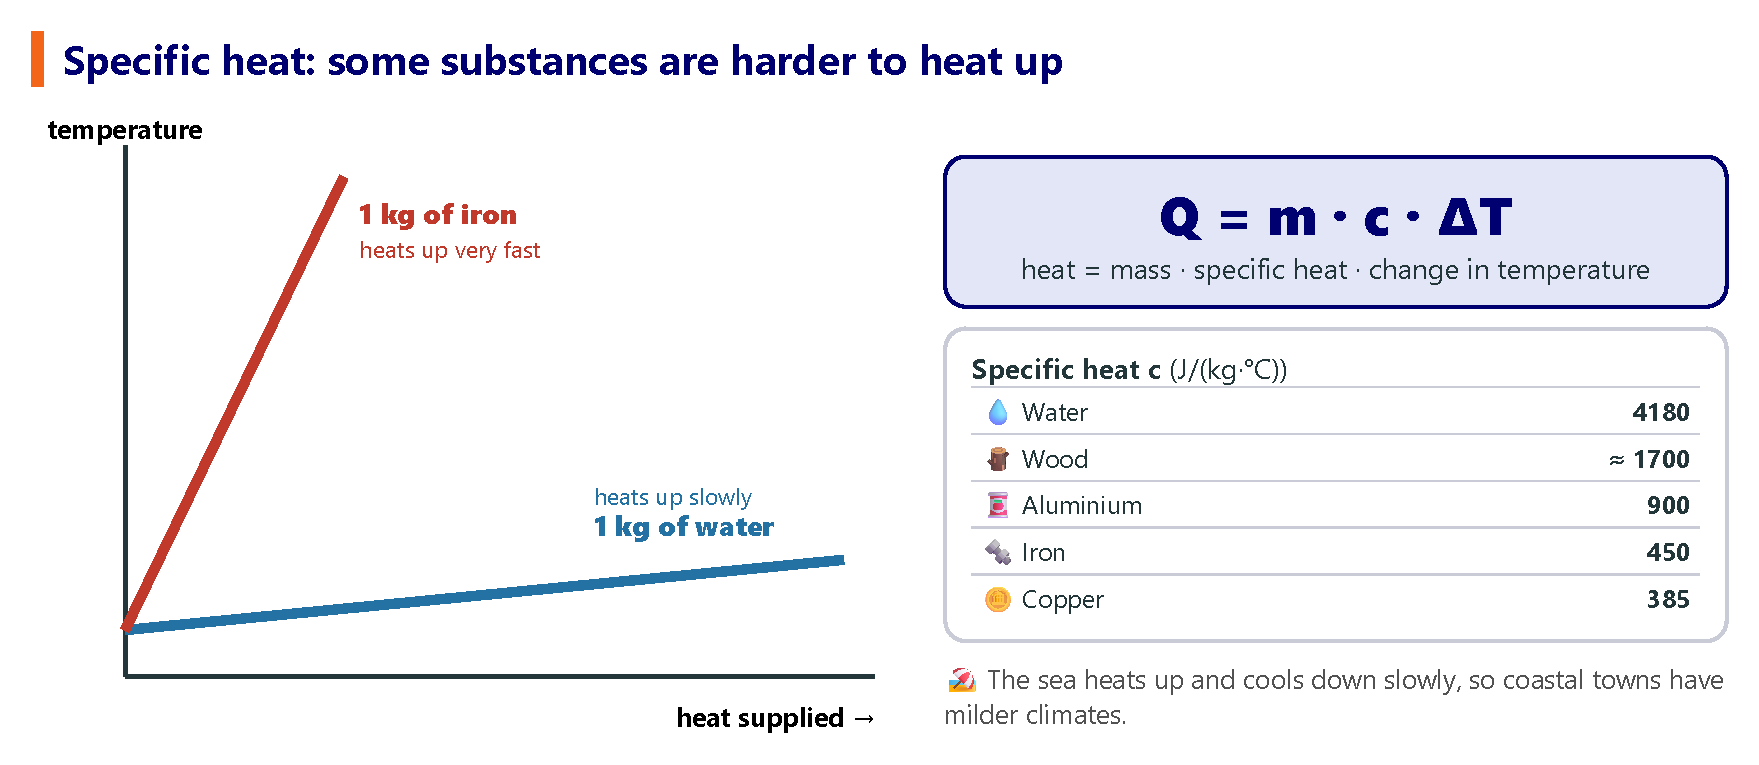
\includegraphics[width=\textwidth]{FigurasSVG/Unit_9_Energy/pdf/specific_heat.pdf}
    \caption{With the same heat, iron gets much hotter than water: water has a very high specific heat.}
    \label{fig:u9_specific_heat}
\end{figure}

\begin{example}
    \textbf{How much heat is needed to raise the temperature of \qty{2}{\kg} of water from \qty{18}{\celsius} to \qty{38}{\celsius}?}
    \begin{equation*}
        Q = m \cdot c \cdot \Delta T = \qty{2}{\kg} \cdot 4180 \dfrac{\text{J}}{\text{kg} \cdot {}^{\circ}\text{C}} \cdot (38 - 18)\ {}^{\circ}\text{C} = \textbf{167 200 J} \approx \textbf{167.2 kJ}
    \end{equation*}
\end{example}

\begin{exercise}
    Calculate the heat needed to raise the temperature of \qty{0.5}{\kg} of water from \qty{15}{\celsius} to \qty{100}{\celsius} in a kettle. Give the answer in kJ and in kcal.
    \begin{solu}
        \(Q = \qty{0.5}{\kg} \cdot 4180 \dfrac{\text{J}}{\text{kg} \cdot {}^{\circ}\text{C}} \cdot (100-15)\ {}^{\circ}\text{C} = \qty{177650}{\joule} \approx \qty{177.65}{\kilo\joule}\). \\
        In kcal: \(\qty{177650}{\joule} \cdot \dfrac{\qty{1}{\calorie}}{\qty{4.18}{\joule}} \approx \qty{42500}{\calorie} \approx \textbf{42.5 kcal}\).
    \end{solu}
\end{exercise}

\begin{exercise}
    A \qty{1.5}{\kg} block of an unknown metal absorbs \qty{13500}{\joule} of heat, and its temperature rises from \qty{20}{\celsius} to \qty{45}{\celsius}. Calculate its specific heat capacity.
    \begin{solu}
        From \(Q = m \cdot c \cdot \Delta T\): \(c = \dfrac{Q}{m \cdot \Delta T} = \dfrac{\qty{13500}{\joule}}{\qty{1.5}{\kg} \cdot (45-20)\ {}^{\circ}\text{C}} = \dfrac{13500}{37.5} = \textbf{360}\ \unit{\joule\per\kg\per\celsius}\).
    \end{solu}
\end{exercise}

\begin{impt}
    \negsubro{Thermal expansion}: most substances increase in volume when their temperature rises, and decrease in volume when it falls: they \textbf{expand} on heating and \textbf{contract} on cooling. Gases expand the most, followed by liquids, and then solids.
\end{impt}

\begin{figure}[H]
    \centering
    % [FIGURA ORIGINAL] \includegraphics[width=\textwidth]{Unit_9/thermal_expansion}
    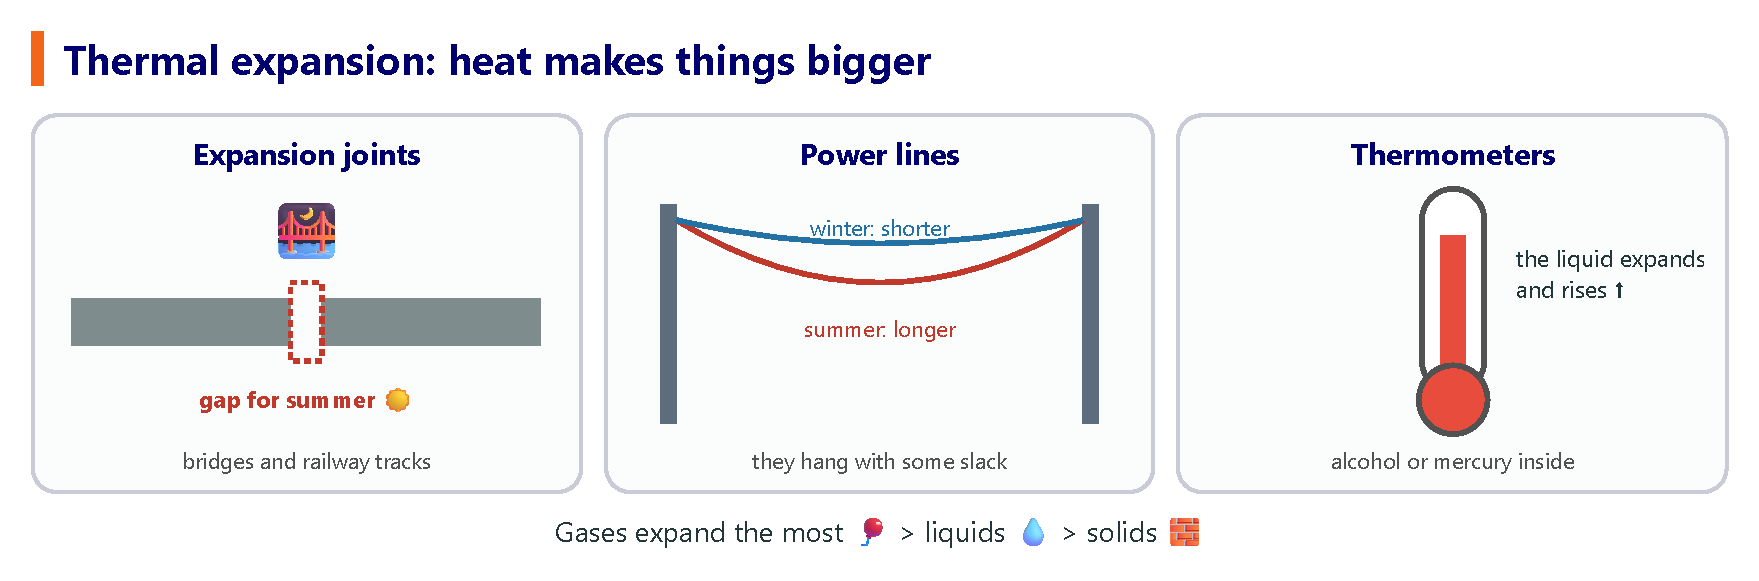
\includegraphics[width=\textwidth]{FigurasSVG/Unit_9_Energy/pdf/thermal_expansion.pdf}
    \caption{Everyday examples of thermal expansion.}
    \label{fig:u9_thermal_expansion}
\end{figure}

\begin{exercise}
    Explain why overhead electrical power lines are hung with some slack between the pylons, instead of being stretched tight.
    \begin{solu}
        In summer, the metal cables heat up and \textbf{expand}, becoming slightly longer; the slack allows this without the cables snapping or being damaged. In winter, the cables cool down and contract again.
    \end{solu}
\end{exercise}

\begin{exercise}
    State whether solids, liquids or gases expand the most when heated, and explain why a hot-air balloon rises when the air inside it is heated.
    \begin{solu}
        \textbf{Gases} expand the most, followed by liquids, and then solids. When the air inside the balloon is heated, it \textbf{expands} and becomes less dense than the cooler air outside; this makes the balloon (and the air inside it) buoyant, so it rises.
    \end{solu}
\end{exercise}

%----------------------------------------------------------------------------------------

\section{Energy sources}

\begin{definition}[Energy source]
    Any material or natural resource that can be used to obtain usable energy.
\end{definition}

\begin{figure}[H]
    \centering
    % [FIGURA ORIGINAL] \includegraphics[width=\textwidth]{Unit_9/sources}
    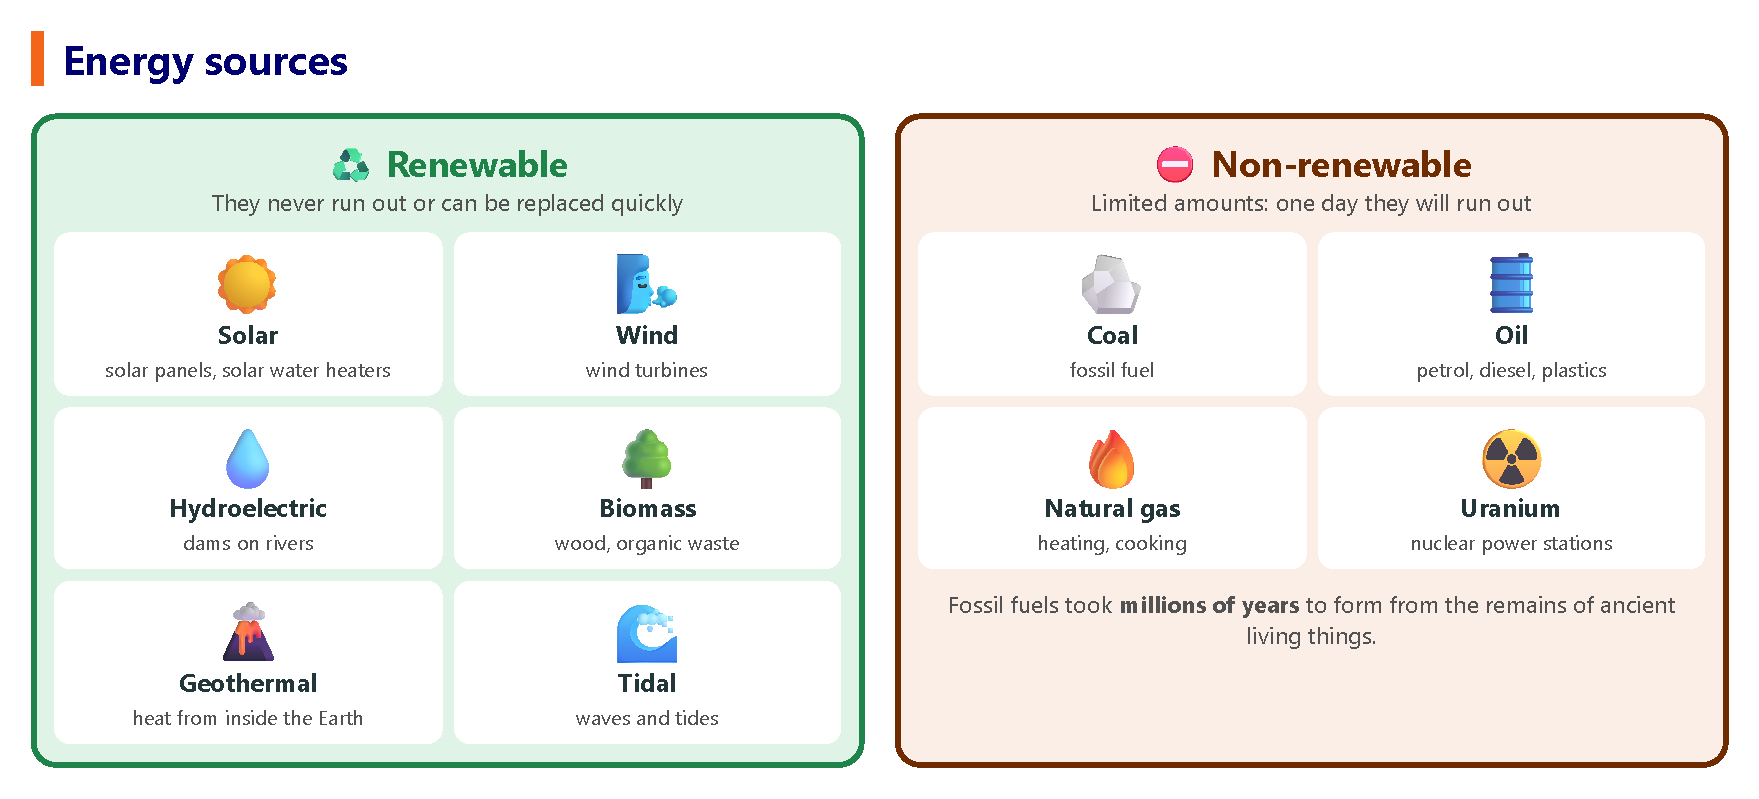
\includegraphics[width=\textwidth]{FigurasSVG/Unit_9_Energy/pdf/sources.pdf}
    \caption{Renewable and non-renewable energy sources.}
    \label{fig:u9_sources}
\end{figure}

\begin{impt}
    \negsubro{Direct use vs.\ electricity generation}: an energy source can be used \textbf{directly} (e.g.\ burning biomass for heating, sunlight heating water) or used to \textbf{generate electricity}, usually by rotating a turbine connected to a generator (in hydroelectric, wind, solar, thermal or nuclear power stations).
\end{impt}

\begin{exercise}
    Classify these energy sources as renewable or non-renewable, and say whether each is used \textbf{directly} or to \textbf{generate electricity}: a) natural gas burnt in a power station; b) firewood burnt in a fireplace; c) sunlight in solar panels that heat water directly; d) uranium in a nuclear power station.
    \begin{solu}
        \begin{enumerate}[label=\alph*)]
            \item Non-renewable; used to generate electricity.
            \item Renewable (biomass); used directly.
            \item Renewable; used directly (no electricity is generated).
            \item Non-renewable; used to generate electricity.
        \end{enumerate}
    \end{solu}
\end{exercise}

\subsection{Wind energy in Castilla-La Mancha}

Castilla-La Mancha is one of the Spanish regions with the largest number of wind farms, thanks to its flat terrain and strong, steady winds. A \negsubro{wind turbine} transforms the \textbf{kinetic energy} of the wind into \textbf{electrical energy}: the wind turns the blades, which rotate a shaft connected to a generator.

\begin{figure}[H]
    \centering
    % [FIGURA ORIGINAL] \includegraphics[width=\textwidth]{Unit_9/wind_turbine}
    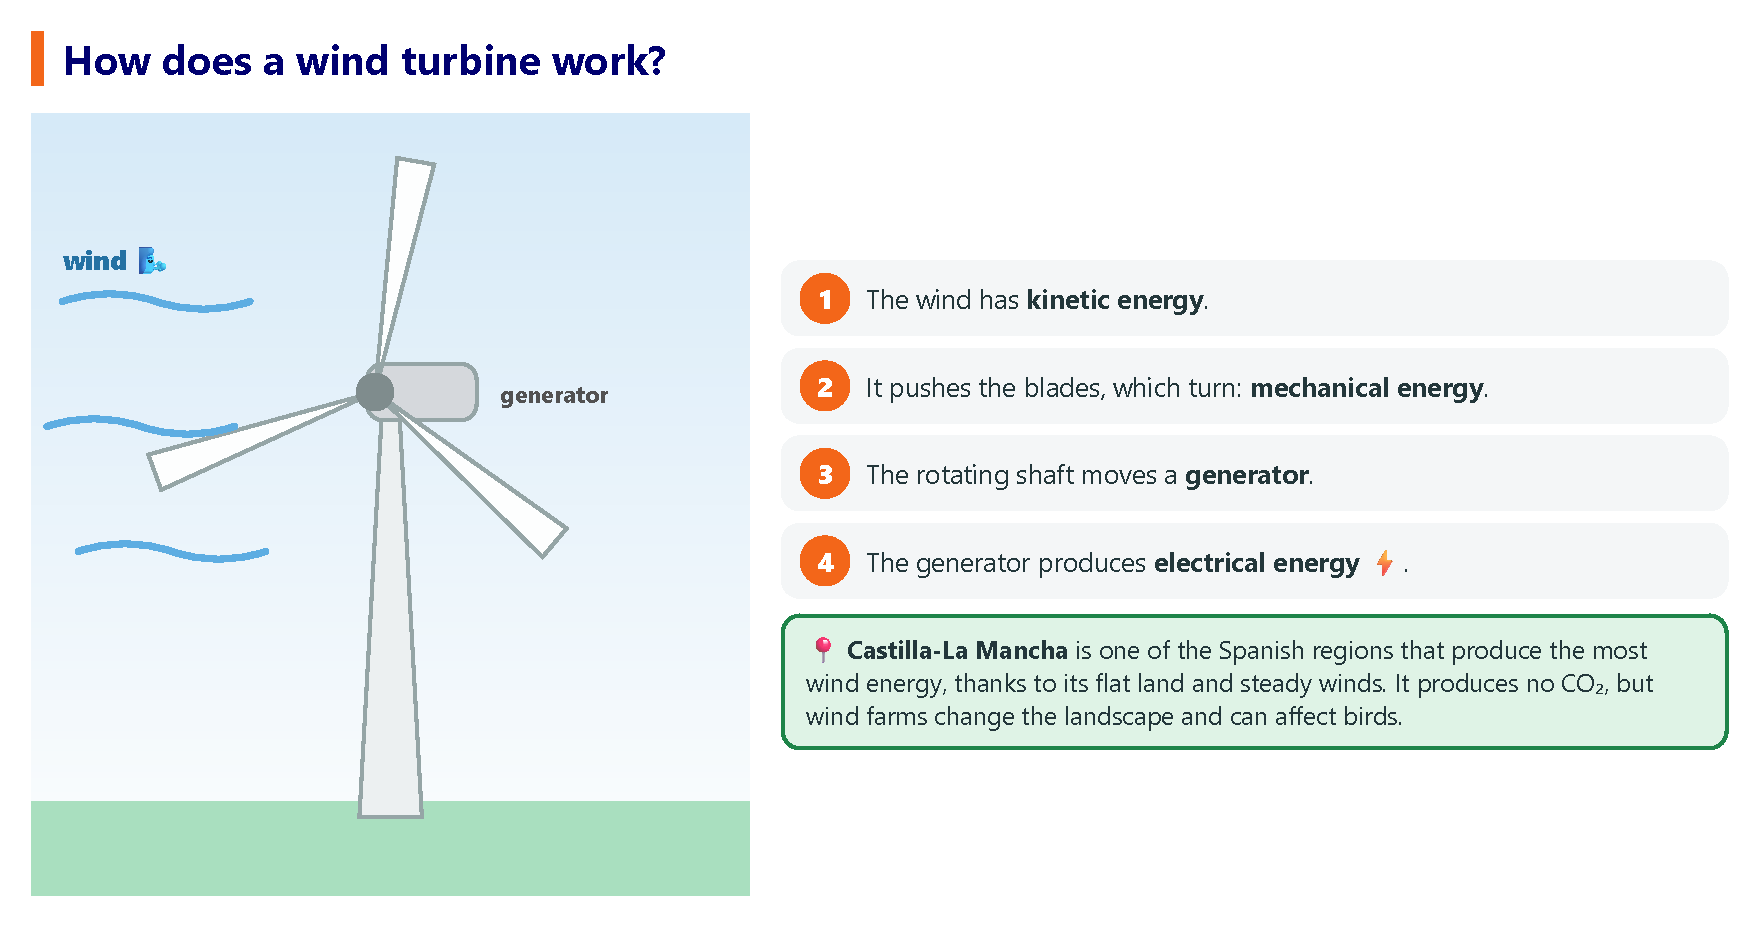
\includegraphics[width=\textwidth]{FigurasSVG/Unit_9_Energy/pdf/wind_turbine.pdf}
    \caption{How a wind turbine transforms the energy of the wind into electricity.}
    \label{fig:u9_wind_turbine}
\end{figure}

\begin{impt}
    \negsubro{Wind power in our region}: wind (eolic) energy is one of the main renewable sources produced in Castilla-La Mancha, together with solar energy, and the region is one of the leading wind-energy producers in Spain. This supplies a large share of the region's electricity without emitting greenhouse gases, but wind farms must be planned carefully, since they can affect birds, bats and the landscape.
\end{impt}

\begin{exercise}
    Explain two advantages and one disadvantage of installing wind farms in Castilla-La Mancha.
    \begin{solu}
        \textbf{Advantages} (any two): wind is a renewable, inexhaustible resource; generating electricity from wind does not emit \ch{CO2} or other pollutants; the region has strong, steady winds, making it an efficient location; it reduces dependence on imported fossil fuels. \\
        \textbf{Disadvantage} (any one): wind turbines change the landscape; they can affect birds and bats; electricity generation depends on the wind blowing, so it is not constant.
    \end{solu}
\end{exercise}

\begin{exercise}
    A wind turbine in Castilla-La Mancha has a rated power of \qty{2}{\mega\watt}. If it operates at full power for \qty{8}{\hour} in a day, calculate the energy it produces that day, in kWh and in MJ.
    \begin{solu}
        \(E = P \cdot t = \qty{2000}{\kilo\watt} \cdot \qty{8}{\hour} = \textbf{16000 kWh}\). \\
        In MJ: \(\qty{16000}{\kwh} \cdot \qty{3.6e6}{\joule\per\kwh} = \qty{5.76e10}{\joule} = \textbf{57600 MJ}\).
    \end{solu}
\end{exercise}

%\subsection{Electrical quantities}
%
%A generator produces an \textbf{electric current} (electric charges moving in an orderly way) inside an \textbf{electric circuit}.
%
%\begin{figure}[H]
%    \centering
%    \includegraphics[width=\textwidth]{Unit_9/circuit}
%    \caption{A simple electric circuit and the three electrical quantities.}
%    \label{fig:u9_circuit}
%\end{figure}
%
%\begin{exercise}
%    Name the basic parts of a simple electric circuit (battery, bulb) and explain the function of each one.
%    \begin{solu}
%        \textbf{Generator} (e.g.\ battery): produces the electric current. \\
%        \textbf{Wires/connectors}: made of a conductive material (e.g.\ copper); transport the current between components. \\
%        \textbf{Switch}: a control element that opens or closes the circuit, stopping or starting the current. \\
%        \textbf{Receiver} (e.g.\ bulb, motor): transforms the electric current into another form of energy (light, movement, etc.).
%    \end{solu}
%\end{exercise}
%
%
%\begin{exercise}
%    A charge of \qty{15}{\coulomb} flows through a wire in \qty{5}{\second}. Calculate the current intensity.
%    \begin{solu}
%        \(I = \dfrac{Q}{t} = \dfrac{\qty{15}{\coulomb}}{\qty{5}{\s}} = \textbf{3 A}\).
%    \end{solu}
%\end{exercise}
%
%\begin{exercise}
%    State which electrical quantity (current intensity, potential difference or resistance) is being described in each case: a) it is measured in volts; b) it opposes the flow of electric current; c) it is measured using an ammeter.
%    \begin{solu}
%        \begin{enumerate}[label=\alph*)]
%            \item Potential difference.
%            \item Resistance.
%            \item Current intensity.
%        \end{enumerate}
%    \end{solu}
%\end{exercise}

%\subsection{Ohm's law}
%
%\begin{impt}
%    \negsubro{Ohm's law} relates the three electrical quantities of a circuit:
%    \begin{equation*}
%        I = \dfrac{\Delta V}{R}
%    \end{equation*}
%    The current intensity through a conductor is directly proportional to the potential difference applied to it, and inversely proportional to its resistance.
%\end{impt}
%
%\begin{figure}[H]
%    \centering
%    \includegraphics[width=\textwidth]{Unit_9/ohm_law}
%    \caption{Ohm's law: the triangle helps us to isolate each quantity.}
%    \label{fig:u9_ohm_law}
%\end{figure}
%
%\begin{example}
%    \textbf{A bulb of resistance \qty{60}{\ohm} is connected to a \qty{12}{\volt} battery. What current flows through it?}
%    \begin{equation*}
%        I = \dfrac{\Delta V}{R} = \dfrac{\qty{12}{\volt}}{\qty{60}{\ohm}} = \textbf{0.2 A}
%    \end{equation*}
%\end{example}
%
%\begin{exercise}
%    A hairdryer connected to the \qty{230}{\volt} mains has a resistance of \qty{46}{\ohm}. Calculate the current intensity that flows through it.
%    \begin{solu}
%        \(I = \dfrac{\Delta V}{R} = \dfrac{\qty{230}{\volt}}{\qty{46}{\ohm}} = \textbf{5 A}\).
%    \end{solu}
%\end{exercise}
%
%\begin{exercise}
%    A current of \qty{0.5}{\ampere} flows through a resistor connected to a \qty{9}{\volt} battery. Calculate the resistance of the resistor.
%    \begin{solu}
%        From Ohm's law, \(R = \dfrac{\Delta V}{I} = \dfrac{\qty{9}{\volt}}{\qty{0.5}{\ampere}} = \textbf{18}\ \Omega\).
%    \end{solu}
%\end{exercise}
%
%\begin{exercise}
%    A resistor has a resistance of \qty{25}{\ohm}. What potential difference must be applied to it so that a current of \qty{2}{\ampere} flows through it?
%    \begin{solu}
%        From Ohm's law, \(\Delta V = I \cdot R = \qty{2}{\ampere} \cdot \qty{25}{\ohm} = \textbf{50 V}\).
%    \end{solu}
%\end{exercise}

%\subsection{Series and parallel circuits}
%
%\begin{figure}[H]
%    \centering
%    \includegraphics[width=\textwidth]{Unit_9/series_parallel}
%    \caption{Bulbs connected in series and in parallel.}
%    \label{fig:u9_series_parallel}
%\end{figure}
%
%\begin{example}
%    A string of old-style Christmas lights wired \textbf{in series} switches off completely if a single bulb breaks. Household electrical installations are wired \textbf{in parallel}: switching off one lamp, or a bulb breaking, does not switch off the other appliances connected to the mains.
%\end{example}
%
%
%\begin{exercise}
%    Say whether the bulbs in each situation are connected in series or in parallel, and justify your answer: a) when one bulb is unscrewed, all the other bulbs go off too; b) a fridge keeps working even if a lamp in another room is switched off.
%    \begin{solu}
%        \begin{enumerate}[label=\alph*)]
%            \item \textbf{Series}: there is a single path for the current, so removing one bulb interrupts the whole circuit.
%            \item \textbf{Parallel}: each appliance is on its own branch, so it works independently of the others.
%        \end{enumerate}
%    \end{solu}
%\end{exercise}
%
%\begin{exercise}
%    Three identical bulbs are connected \textbf{in series} to a \qty{12}{\volt} battery. If one bulb burns out, what happens to the other two? Explain.
%    \begin{solu}
%        In a series circuit there is only \textbf{one path} for the current. If one bulb burns out, it interrupts that path, so no current can flow anywhere in the circuit: the \textbf{other two bulbs also go off}.
%    \end{solu}
%\end{exercise}
%
%\begin{exercise}
%    Two lamps with different resistances are connected \textbf{in parallel} to the \qty{230}{\volt} mains supply. Explain why both lamps are subject to the same potential difference, and what this means for their brightness.
%    \begin{solu}
%        In a parallel circuit, every branch connects the same two points, so the potential difference across each branch equals the source voltage: both lamps have \qty{230}{\volt} across them. However, by Ohm's law (\(I = \Delta V / R\)), the lamp with the \textbf{lower resistance} draws a \textbf{higher current}, so it will shine \textbf{brighter}, even though both receive the same potential difference.
%    \end{solu}
%\end{exercise}

%----------------------------------------------------------------------------------------

\section{The environmental impact of energy}

Obtaining, transporting and using energy has consequences for the environment: resources are depleted, toxic waste is produced, and air, water and soil are polluted.

\begin{itemize}
    \item \negsubro{Acid rain}: when fossil fuels are burnt, the substances released combine with rainwater; this rain damages plants and can affect areas far from where the pollution was produced.
    \item \negsubro{Global warming}: burning fossil fuels increases the carbon dioxide in the atmosphere, which increases the natural greenhouse effect and raises the planet's average temperature.
\end{itemize}

\begin{table}[H]
    \centering
    \begin{tabular}{p{5.3cm}p{5.3cm}}
        \toprule
        \textbf{Renewable sources} & \textbf{Non-renewable sources} \\
        \midrule
        Do not emit harmful substances, but they can greatly change the landscape and the habitats of living things (e.g.\ wind turbines, large solar or hydroelectric power plants). &
        Fossil fuels emit \ch{CO2} and other greenhouse gases, and cause acid rain; extraction changes the land, and accidental spills cause pollution. Radioactive materials produce dangerous waste that must be stored securely. \\
        \bottomrule
    \end{tabular}
    \caption{Environmental impact of renewable and non-renewable energy sources.}
    \label{tab:u9_impact}
\end{table}

\begin{exercise}
    Match each cause with its environmental consequence: a) burning fossil fuels for transport; b) an oil tanker accident; c) a nuclear power station's radioactive waste. \newline
    Consequences: 1. large oil spills; 2. air pollution / global warming; 3. long-term, dangerous waste storage needs.
    \begin{solu}
        a) \(\to\) 2; \quad b) \(\to\) 1; \quad c) \(\to\) 3.
    \end{solu}
\end{exercise}

\begin{exercise}
    Explain how burning fossil fuels contributes to two different environmental problems studied in this unit.
    \begin{solu}
        Burning fossil fuels releases \ch{CO2}, which increases the natural \textbf{greenhouse effect} and causes \textbf{global warming}. It also releases sulfur and nitrogen oxides, which combine with water in the atmosphere and fall as \textbf{acid rain}, damaging plants and ecosystems, sometimes far from where the pollution was originally produced.
    \end{solu}
\end{exercise}

%----------------------------------------------------------------------------------------

\section{The energy we use}

\begin{itemize}
    \item \negsubro{Primary energy}: energy obtained directly from a source in nature (e.g.\ the chemical energy in coal, or the kinetic energy of wind), used directly or transformed.
    \item \negsubro{Final energy}: the energy that is actually supplied to and used by the consumer (e.g.\ electricity, petrol), after it has been transformed and transported.
\end{itemize}

\begin{impt}
    A country that consumes more energy than it produces is an \negsubro{energy importer}; a country that produces more than it consumes is an \negsubro{energy exporter}.
\end{impt}

Figure~\ref{fig:u9_energy_mix} shows the world energy mix by primary source in 2021, used in the exercise below.

\begin{figure}[H]
    \centering
    % [FIGURA ORIGINAL] \includegraphics[width=0.95\textwidth]{Unit_9/energy_mix}
    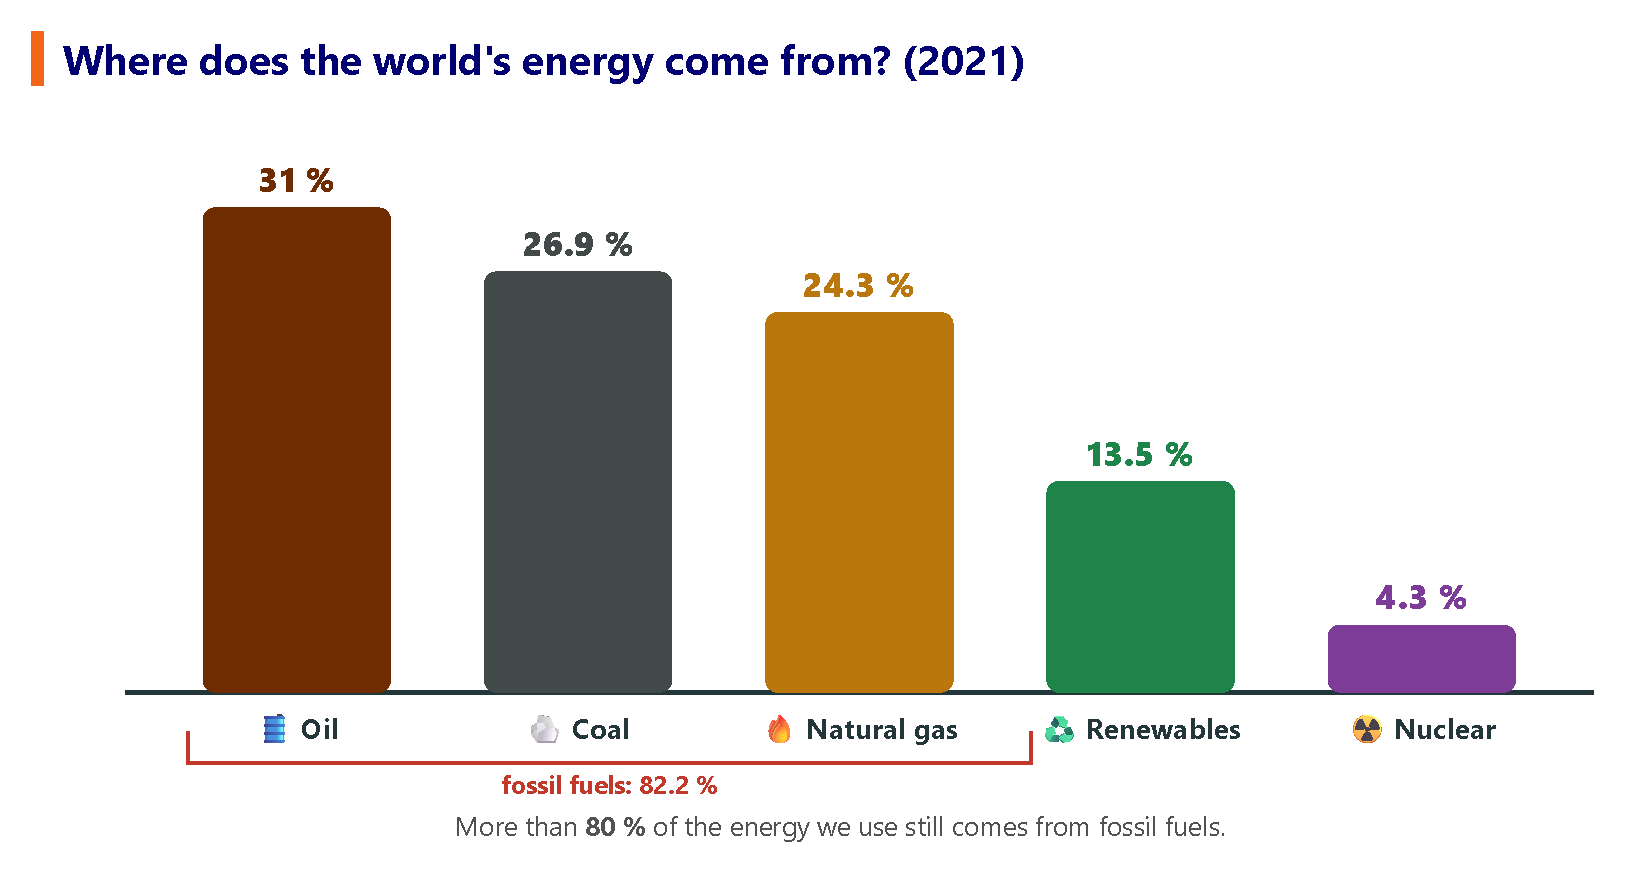
\includegraphics[width=0.95\textwidth]{FigurasSVG/Unit_9_Energy/pdf/energy_mix.pdf}
    \caption{World primary energy consumption by source, 2021.}
    \label{fig:u9_energy_mix}
\end{figure}

\begin{exercise}
    Worldwide in 2021, total energy consumption by primary source was distributed as follows: petroleum 31\,\%, natural gas 24.3\,\%, coal 26.9\,\%, nuclear 4.3\,\%, renewables 13.5\,\%, out of a total of \num{14220} Mtoe (million tonnes of oil equivalent). Calculate the amount of energy, in Mtoe, consumed from petroleum and from renewables.
    \begin{solu}
        Petroleum: \(14220 \cdot \dfrac{31}{100} \approx 4408.2\) Mtoe. \\
        Renewables: \(14220 \cdot \dfrac{13.5}{100} \approx 1919.7\) Mtoe.
    \end{solu}
\end{exercise}

\begin{exercise}
    Explain why electrical energy appears in the \textbf{final} energy consumption of a country, but not directly in its \textbf{primary} energy consumption.
    \begin{solu}
        Electricity is not a primary energy source itself; it is generated by transforming primary sources (fossil fuels, nuclear, wind, water, sun, etc.). Once generated, it is counted as a form of \textbf{final} energy, since it is what is actually delivered to and used by the consumer.
    \end{solu}
\end{exercise}

\begin{exercise}
    A country produced 145 Mtoe of primary energy in a given year but consumed 165 Mtoe. Was that country an energy importer or an energy exporter that year? Justify your answer and calculate the energy deficit, in Mtoe.
    \begin{solu}
        Since consumption (165 Mtoe) is greater than production (145 Mtoe), the country was an \textbf{energy importer} that year: it needed to bring in energy from abroad to cover its needs. \\
        Deficit \(= 165 - 145 = \textbf{20 Mtoe}\).
    \end{solu}
\end{exercise}

%----------------------------------------------------------------------------------------

\section{Energy saving and sustainable development}

\begin{definition}[Sustainable development]
    Development that meets present energy needs without wasting resources or causing unnecessary environmental damage, so that future generations can also meet their needs.
\end{definition}

\begin{itemize}
    \item \negsubro{Design of efficient products and buildings}: energy-efficient vehicles and appliances; well-insulated houses to prevent energy losses.
    \item \negsubro{Local energy sources}: installing solar panels; using the natural course of rivers; using local organic waste as biomass.
    \item \negsubro{Avoiding unnecessary consumption}: using public transport; buying only what is needed; consuming local products.
    \item \negsubro{At home}: use energy-saving light bulbs; switch off lights and devices when not in use; use heating and air conditioning sensibly; do not waste hot water.
\end{itemize}

\begin{figure}[H]
    \centering
    % [FIGURA ORIGINAL] \includegraphics[width=\textwidth]{Unit_9/energy_saving}
    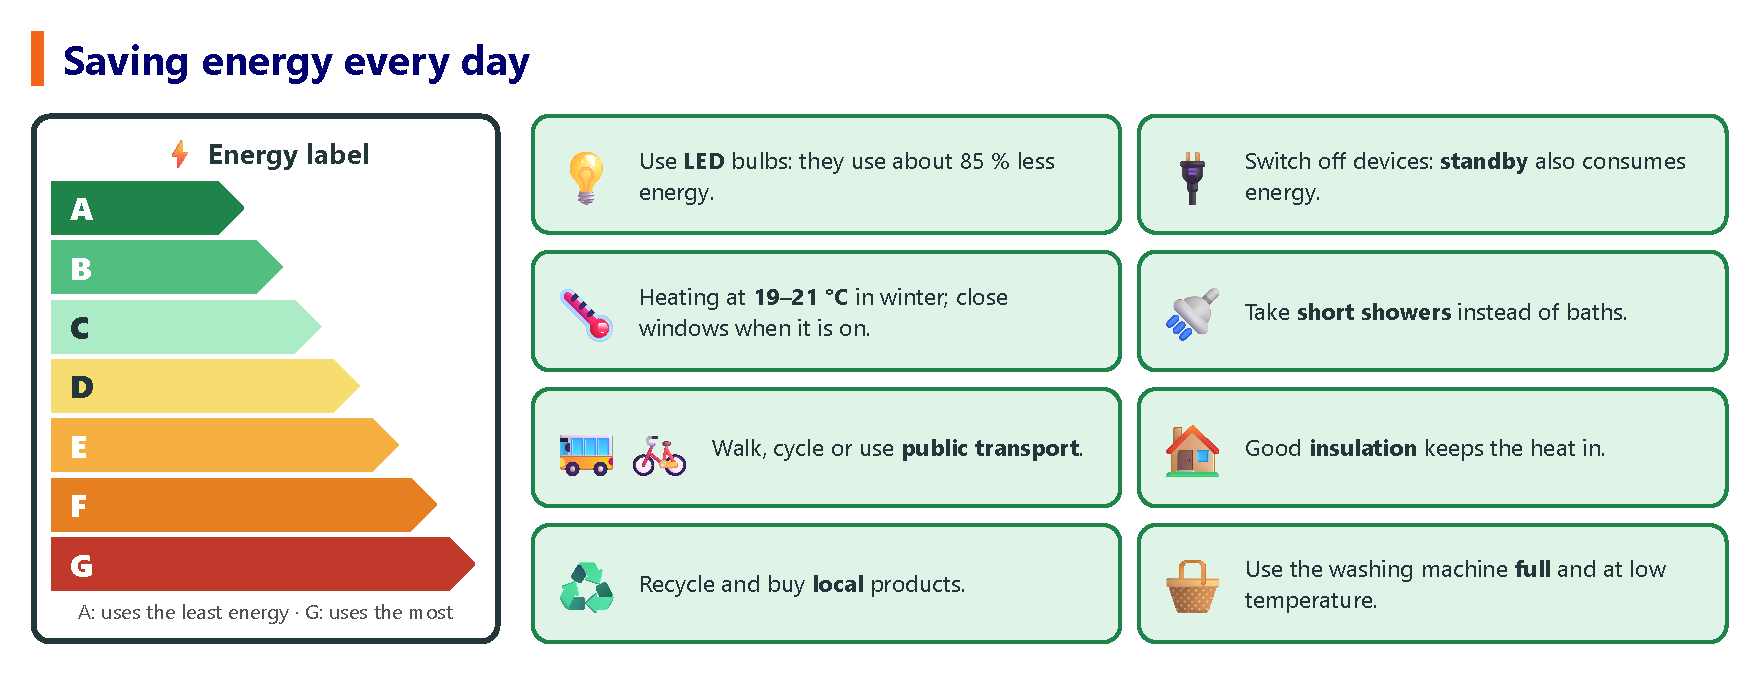
\includegraphics[width=\textwidth]{FigurasSVG/Unit_9_Energy/pdf/energy_saving.pdf}
    \caption{The energy label and some simple ways to save energy.}
    \label{fig:u9_energy_saving}
\end{figure}

\begin{exercise}
    A category D fridge (average consumption) uses \qty{600}{\kwh} per year. Category A fridges consume about 55\,\% \textbf{less} than average, and category G fridges consume about 125\,\% \textbf{more} than average.
    \begin{enumerate}[label=\letraminuscula]
        \item How much would a category A fridge consume per year?
        \item How much would a category G fridge consume per year?
    \end{enumerate}
    \begin{solu}
        \begin{enumerate}[label=\alph*)]
            \item \(\qty{600}{\kwh} \cdot (1 - 0.55) = 600 \cdot 0.45 = \qty{270}{\kwh}\) per year.
            \item \(\qty{600}{\kwh} \cdot (1 + 1.25) = 600 \cdot 2.25 = \qty{1350}{\kwh}\) per year.
        \end{enumerate}
    \end{solu}
\end{exercise}

\begin{exercise}
    Decide whether each action saves energy, and explain why: a) unplugging electrical devices that are not in use; b) opening windows in winter for ventilation while the heating is on; c) using energy-saving light bulbs.
    \begin{solu}
        \begin{enumerate}[label=\alph*)]
            \item \textbf{Saves energy}: many devices keep consuming small amounts of electricity on standby.
            \item \textbf{Does not save energy} (if done with the heating on): heat escapes and the heating has to work harder to compensate. (Brief ventilation with the heating \textit{off} is fine.)
            \item \textbf{Saves energy}: LED/energy-saving bulbs turn a higher percentage of the electrical energy into light and less into wasted heat, i.e.\ they degrade less energy.
        \end{enumerate}
    \end{solu}
\end{exercise}

\begin{exercise}
    A family replaces 10 incandescent light bulbs (\qty{60}{\watt} each) with 10 LED bulbs (\qty{9}{\watt} each), used for an average of \qty{4}{\hour} per day. Calculate the energy saved per day, in kWh.
    \begin{solu}
        Incandescent bulbs: \(10 \cdot \qty{60}{\watt} = \qty{600}{\watt} = \qty{0.6}{\kilo\watt}\); \(\qty{0.6}{\kilo\watt} \cdot \qty{4}{\hour} = \qty{2.4}{\kwh}\). \\
        LED bulbs: \(10 \cdot \qty{9}{\watt} = \qty{90}{\watt} = \qty{0.09}{\kilo\watt}\); \(\qty{0.09}{\kilo\watt} \cdot \qty{4}{\hour} = \qty{0.36}{\kwh}\). \\
        Energy saved \(= 2.4 - 0.36 = \textbf{2.04 kWh per day}\).
    \end{solu}
\end{exercise}

%----------------------------------------------------------------------------------------

\section*{Summary}

\begin{itemize}
    \item \textbf{Energy}: the capacity of a body to produce changes; measured in joules (also kJ, cal, kWh, toe).
    \item \textbf{Forms of energy}: kinetic, potential (gravitational and elastic), mechanical, thermal, electrical, radiant, chemical and nuclear.
    \item \textbf{Properties}: energy can be transferred, stored, transported and transformed; it is always conserved (as a total) but part of it is degraded (turned into unusable heat) every time it is transformed.
    \item \textbf{Effects of heat}: specific heat \(c\) measures the heat needed to raise \qty{1}{\kg} of a substance by \qty{1}{\celsius} (\(Q = mc\Delta T\)); most substances expand when heated and contract when cooled (thermal expansion).
    \item \textbf{Energy sources}: renewable (wind, water, sun, biomass, geothermal) do not run out; non-renewable (fossil fuels, radioactive materials) are limited and eventually run out. Wind energy is one of the main renewable sources produced in Castilla-La Mancha.
%    \item \textbf{Electrical quantities}: current intensity \(I\) (A), potential difference \(\Delta V\) (V) and resistance \(R\) (\(\Omega\)), related by \textbf{Ohm's law}, \(I = \Delta V / R\). Circuits can be wired in \textbf{series} (single path) or in \textbf{parallel} (independent branches).
    \item \textbf{Environmental impact}: burning fossil fuels causes acid rain and global warming; all energy sources have some impact on the landscape or habitats.
    \item \textbf{Primary vs.\ final energy}: primary energy comes directly from a source; final energy is what is actually delivered to and used by the consumer (e.g.\ electricity).
    \item \textbf{Sustainable development}: saving energy and using efficient, local and renewable resources to meet our needs without compromising future generations.
\end{itemize}

\section{Vocabulary}

\begin{vocabulary}[Energy]
    A physical quantity that measures the capacity of a body to produce changes in itself or in other bodies. \newline
    \textbf{Translation to Spanish}: Energía
\end{vocabulary}

\begin{vocabulary}[Kinetic energy]
    Energy a body has because it is moving. \newline
    \textbf{Translation to Spanish}: Energía cinética
\end{vocabulary}

\begin{vocabulary}[Potential energy]
    Energy a body has because of its position or state (e.g.\ its height, or being stretched). \newline
    \textbf{Translation to Spanish}: Energía potencial
\end{vocabulary}

\begin{vocabulary}[Energy source]
    Any material or natural resource that can be used to obtain usable energy. \newline
    \textbf{Translation to Spanish}: Fuente de energía
\end{vocabulary}

\begin{vocabulary}[Renewable]
    An energy source whose resources can be replaced after use, or that never run out. \newline
    \textbf{Translation to Spanish}: Renovable
\end{vocabulary}

\begin{vocabulary}[Non-renewable]
    An energy source whose resources are limited and cannot be replaced once consumed. \newline
    \textbf{Translation to Spanish}: No renovable
\end{vocabulary}

\begin{vocabulary}[Electric current]
    Electric charges moving in an orderly way through a conductor. \newline
    \textbf{Translation to Spanish}: Corriente eléctrica
\end{vocabulary}

\begin{vocabulary}[Specific heat capacity]
    The amount of heat needed to raise the temperature of \qty{1}{\kg} of a substance by \qty{1}{\celsius}. \newline
    \textbf{Translation to Spanish}: Calor específico
\end{vocabulary}

\begin{vocabulary}[Thermal expansion]
    The increase in volume of a substance when its temperature rises. \newline
    \textbf{Translation to Spanish}: Dilatación térmica
\end{vocabulary}

\begin{vocabulary}[Wind energy]
    Kinetic energy of the wind, used directly or transformed into electrical energy by wind turbines. \newline
    \textbf{Translation to Spanish}: Energía eólica
\end{vocabulary}

\begin{vocabulary}[Ohm's law]
    The relationship between current intensity, potential difference and resistance in a circuit: \(I = \Delta V / R\). \newline
    \textbf{Translation to Spanish}: Ley de Ohm
\end{vocabulary}

\begin{vocabulary}[Series circuit]
    A circuit in which components are connected one after another along a single path. \newline
    \textbf{Translation to Spanish}: Circuito en serie
\end{vocabulary}

\begin{vocabulary}[Parallel circuit]
    A circuit in which components are connected on separate branches between the same two points. \newline
    \textbf{Translation to Spanish}: Circuito en paralelo
\end{vocabulary}

\begin{vocabulary}[Energy degradation]
    The loss, during any energy transformation, of part of the energy as unusable heat. \newline
    \textbf{Translation to Spanish}: Degradación de la energía
\end{vocabulary}

\begin{vocabulary}[Primary energy]
    Energy obtained directly from a natural source. \newline
    \textbf{Translation to Spanish}: Energía primaria
\end{vocabulary}

\begin{vocabulary}[Final energy]
    The energy actually supplied to and used by the consumer. \newline
    \textbf{Translation to Spanish}: Energía final
\end{vocabulary}

\begin{vocabulary}[Sustainable development]
    Development that meets present needs without compromising the ability of future generations to meet theirs. \newline
    \textbf{Translation to Spanish}: Desarrollo sostenible
\end{vocabulary}




%----------------------------------------------------------------------------------------
%	SECTIONING EXAMPLES CHAPTER
%----------------------------------------------------------------------------------------

    %\chapterimage{orange3b} % Chapter heading image % --- imagen antigua ---
    \chapterimage{images/portada_cabeceras/cabecera_general} % Cabecera nueva (las de cada unidad van antes de cada \chapter)
    \chapterspaceabove{6.75cm} % Whitespace from the top of the page to the chapter title on chapter pages
    \chapterspacebelow{7.25cm} % Amount of vertical whitespace from the top margin to the start of the text on chapter pages


%----------------------------------------------------------------------------------------
%	Tablas Periódicas
%----------------------------------------------------------------------------------------


    \part{Tabla Periódica}

    \newpage
    \pagestyle{empty}
    \begin{landscape}
        \begin{figure}[H]
            \centering
            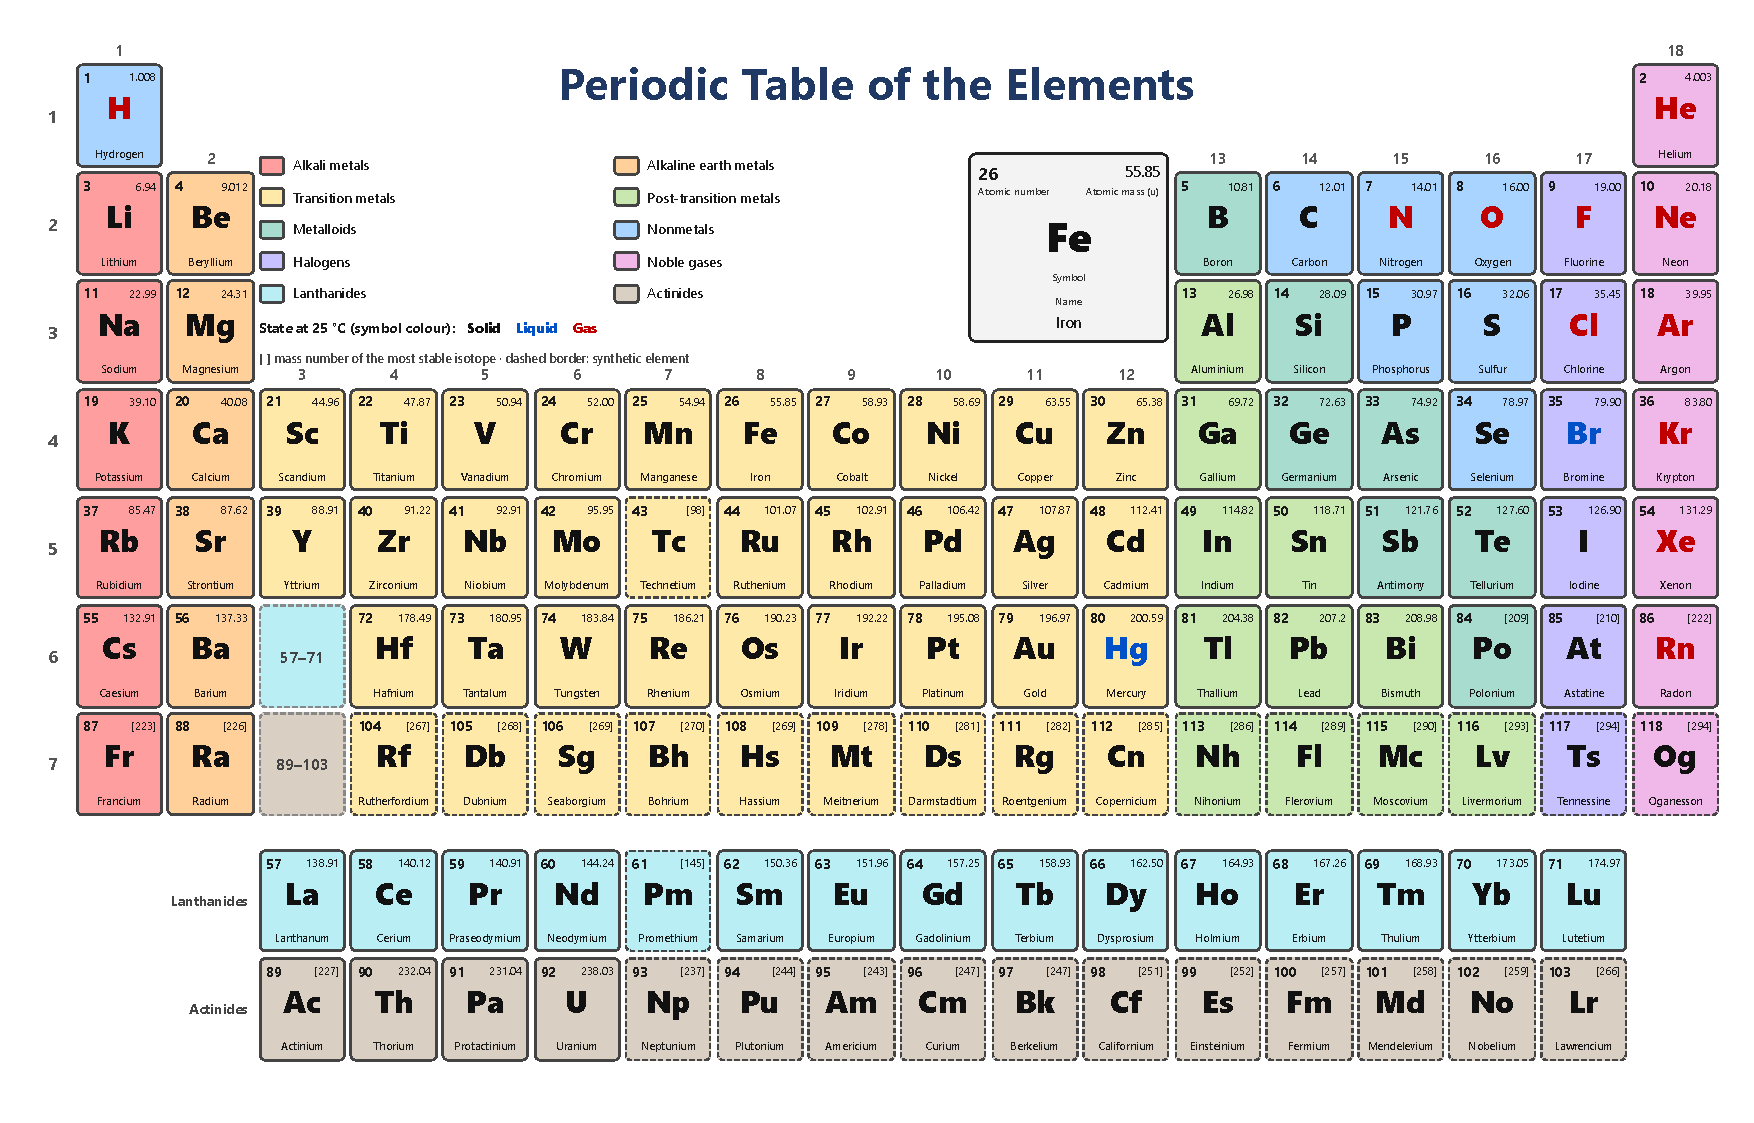
\includegraphics[width=\linewidth,height=0.85\textheight,keepaspectratio]{images/SP_atomo/2_3_ESO_TP_EN_html}
            \caption{Periodic Table of Elements}
            \label{fig:periodic_table}
        \end{figure}
    \end{landscape}
    \newpage
    \begin{landscape}
        \begin{figure}[H]
            \centering
            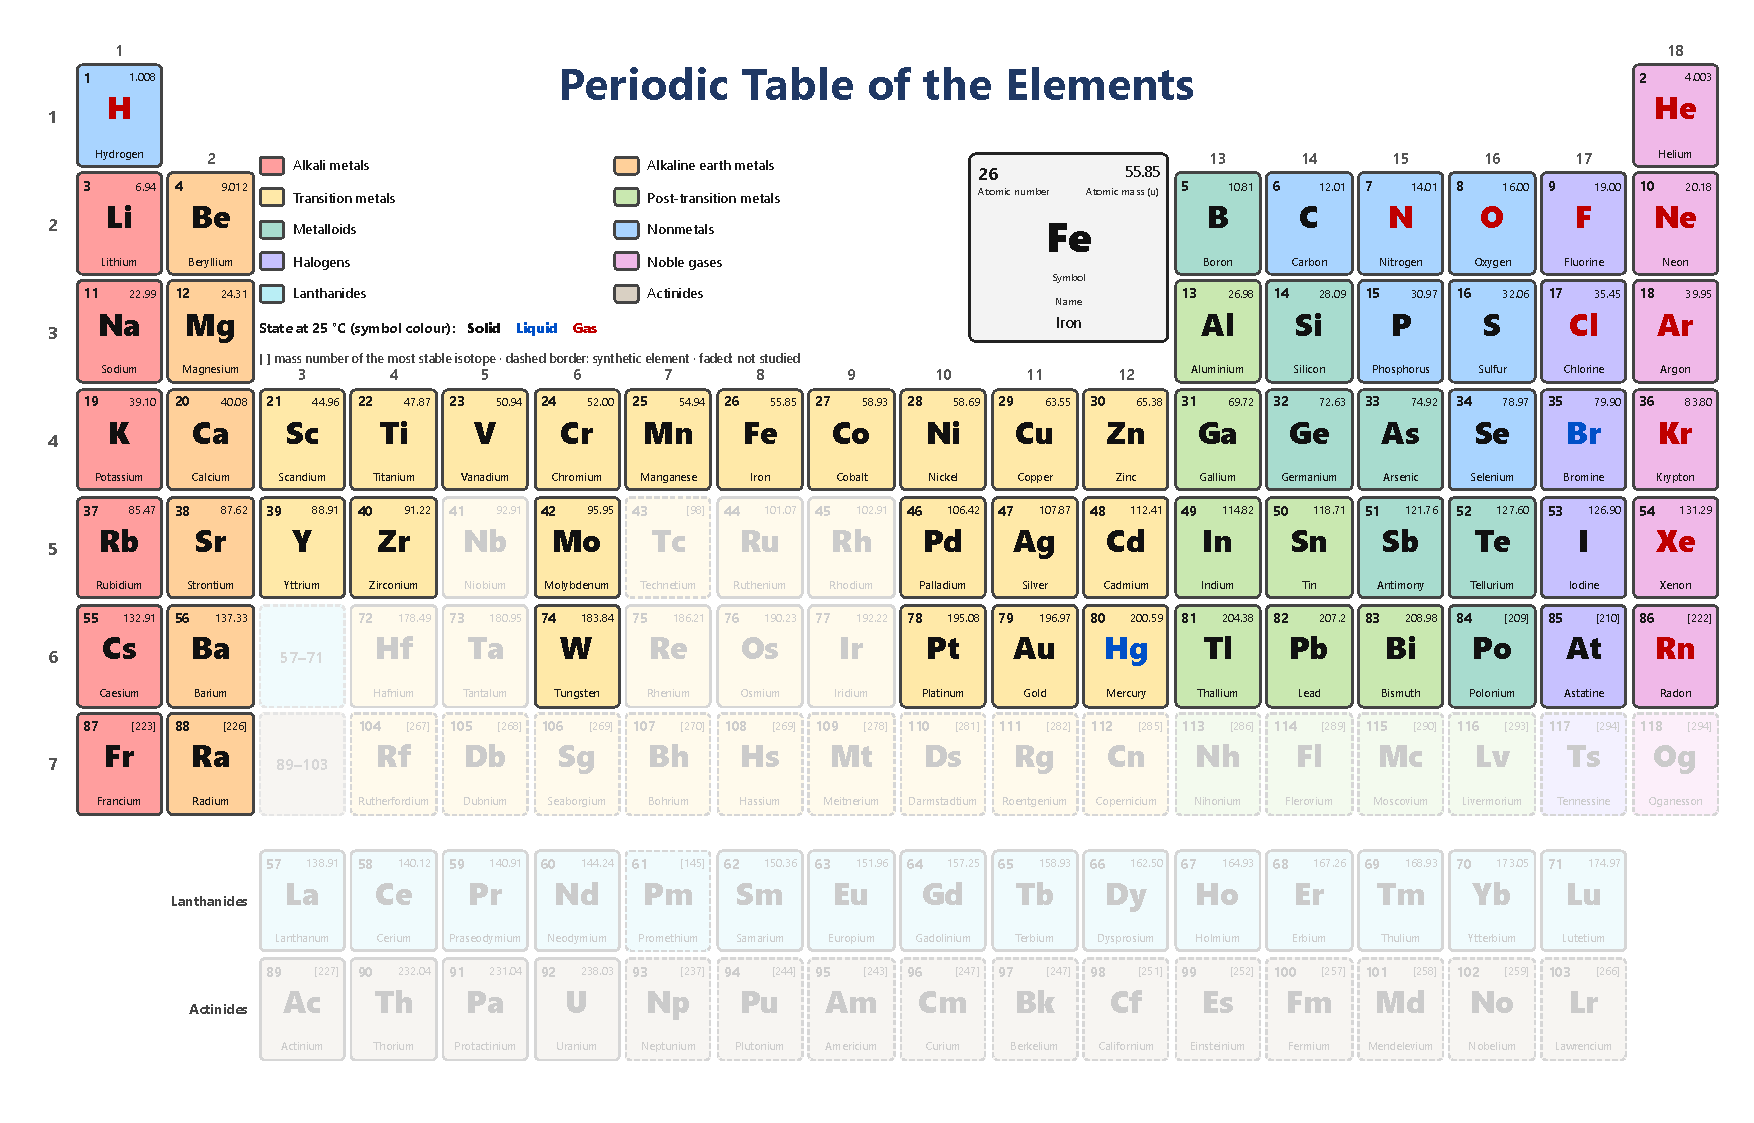
\includegraphics[width=\linewidth,height=0.85\textheight,keepaspectratio]{images/SP_atomo/2_3_ESO_TP_EN_reducida_html}
            \caption{Periodic Table of Elements (2º ESO)}
            \label{fig:periodic_table_reducida}
        \end{figure}
    \end{landscape}
    \newpage
    \begin{landscape}
        \begin{figure}[H]
            \centering
            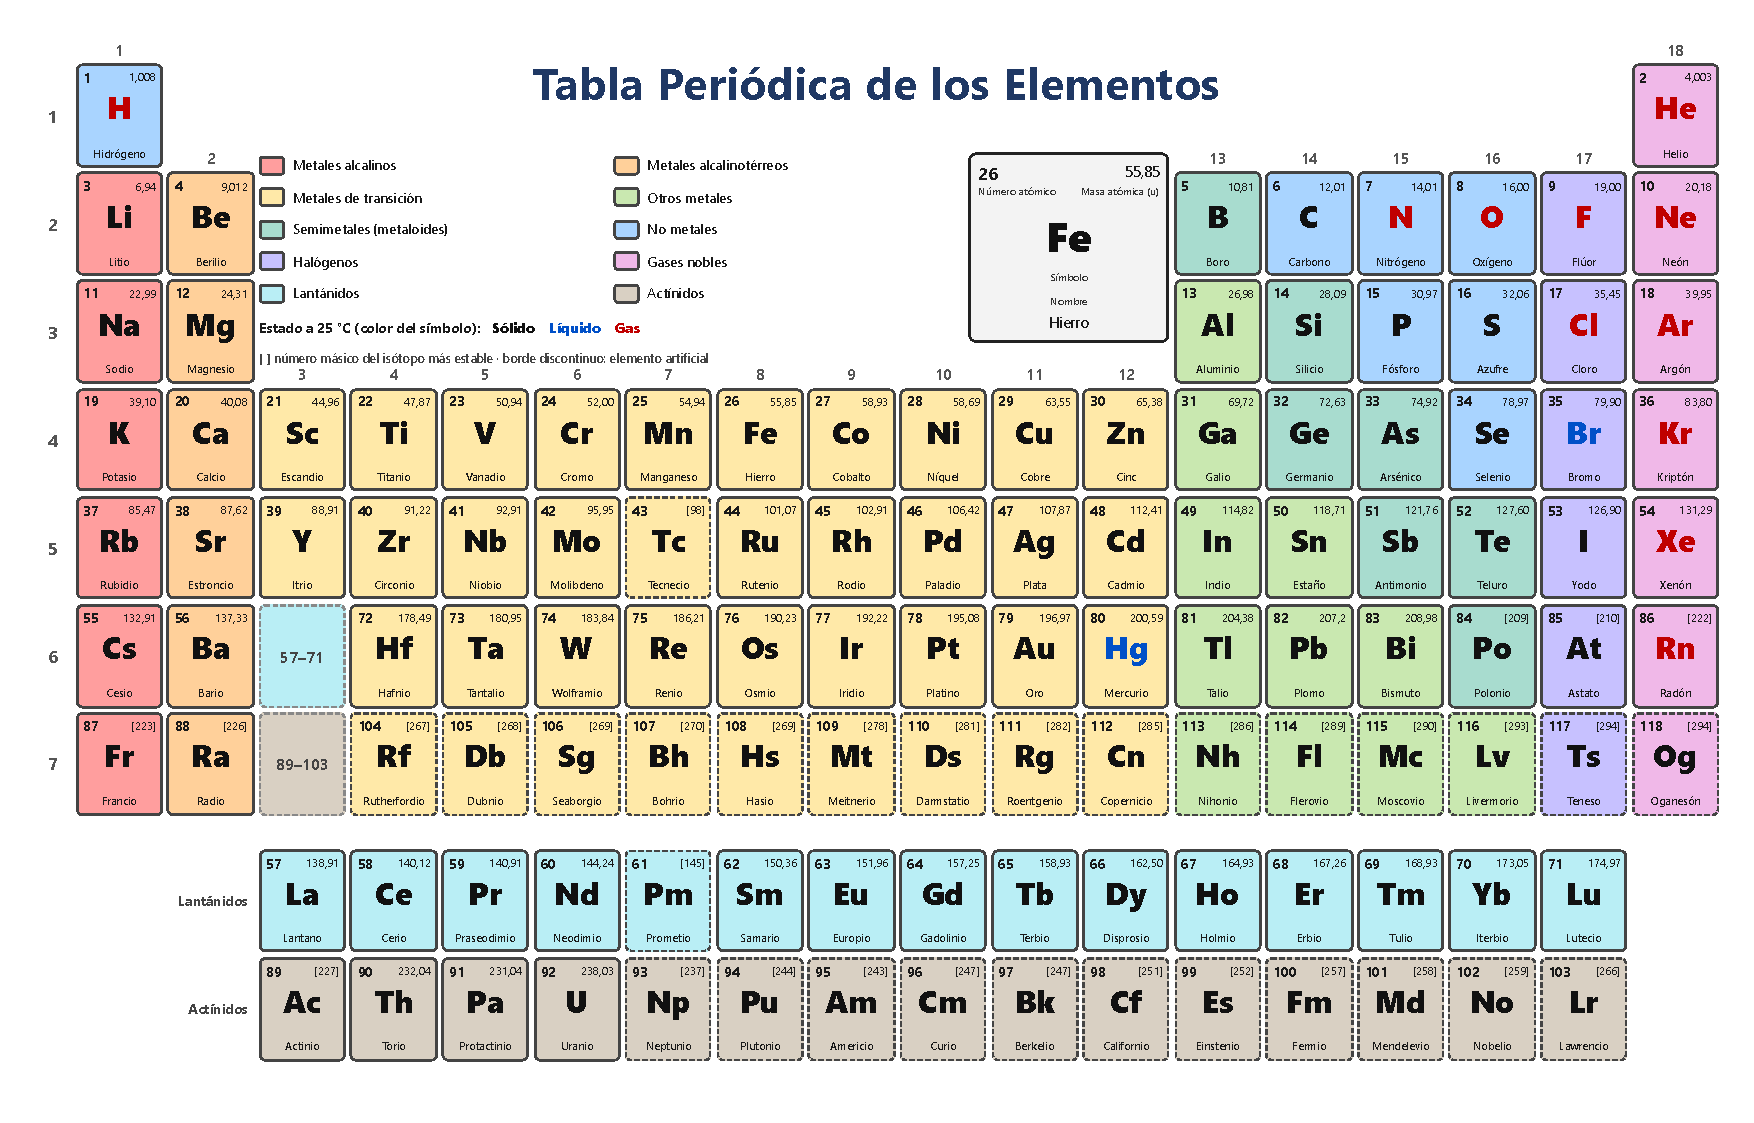
\includegraphics[width=\linewidth,height=0.85\textheight,keepaspectratio]{images/SP_atomo/2_3_ESO_TP_ES_html}
            \caption{Tabla Periódica de los elementos}
            \label{fig:tabla_periodica}
        \end{figure}
    \end{landscape}
    \newpage
    \begin{landscape}
        \begin{figure}[H]
            \centering
            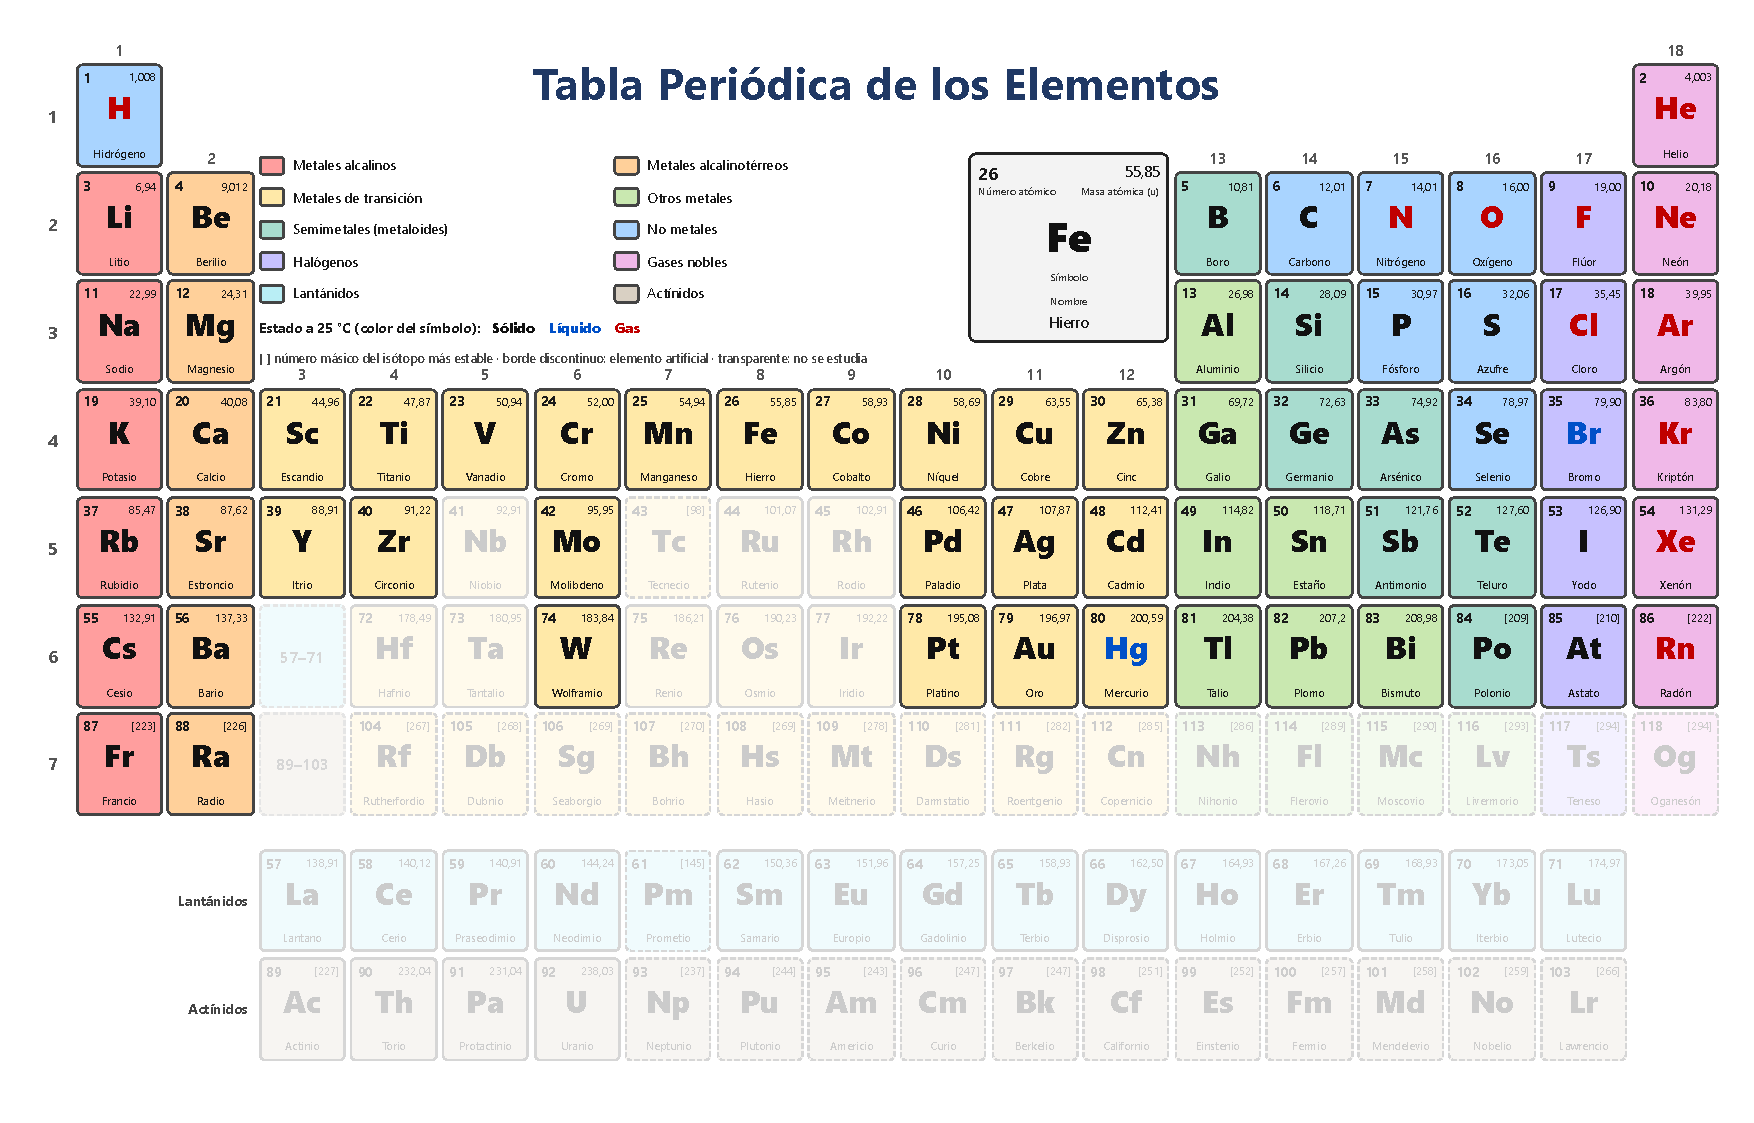
\includegraphics[width=\linewidth,height=0.85\textheight,keepaspectratio]{images/SP_atomo/2_3_ESO_TP_ES_reducida_html}
            \caption{Tabla Periódica de los elementos (2º ESO)}
            \label{fig:tabla_periodica_reducida}
        \end{figure}
    \end{landscape}

    \newpage

    \begin{landscape}

    \begin{figure}[H]
        \centering
        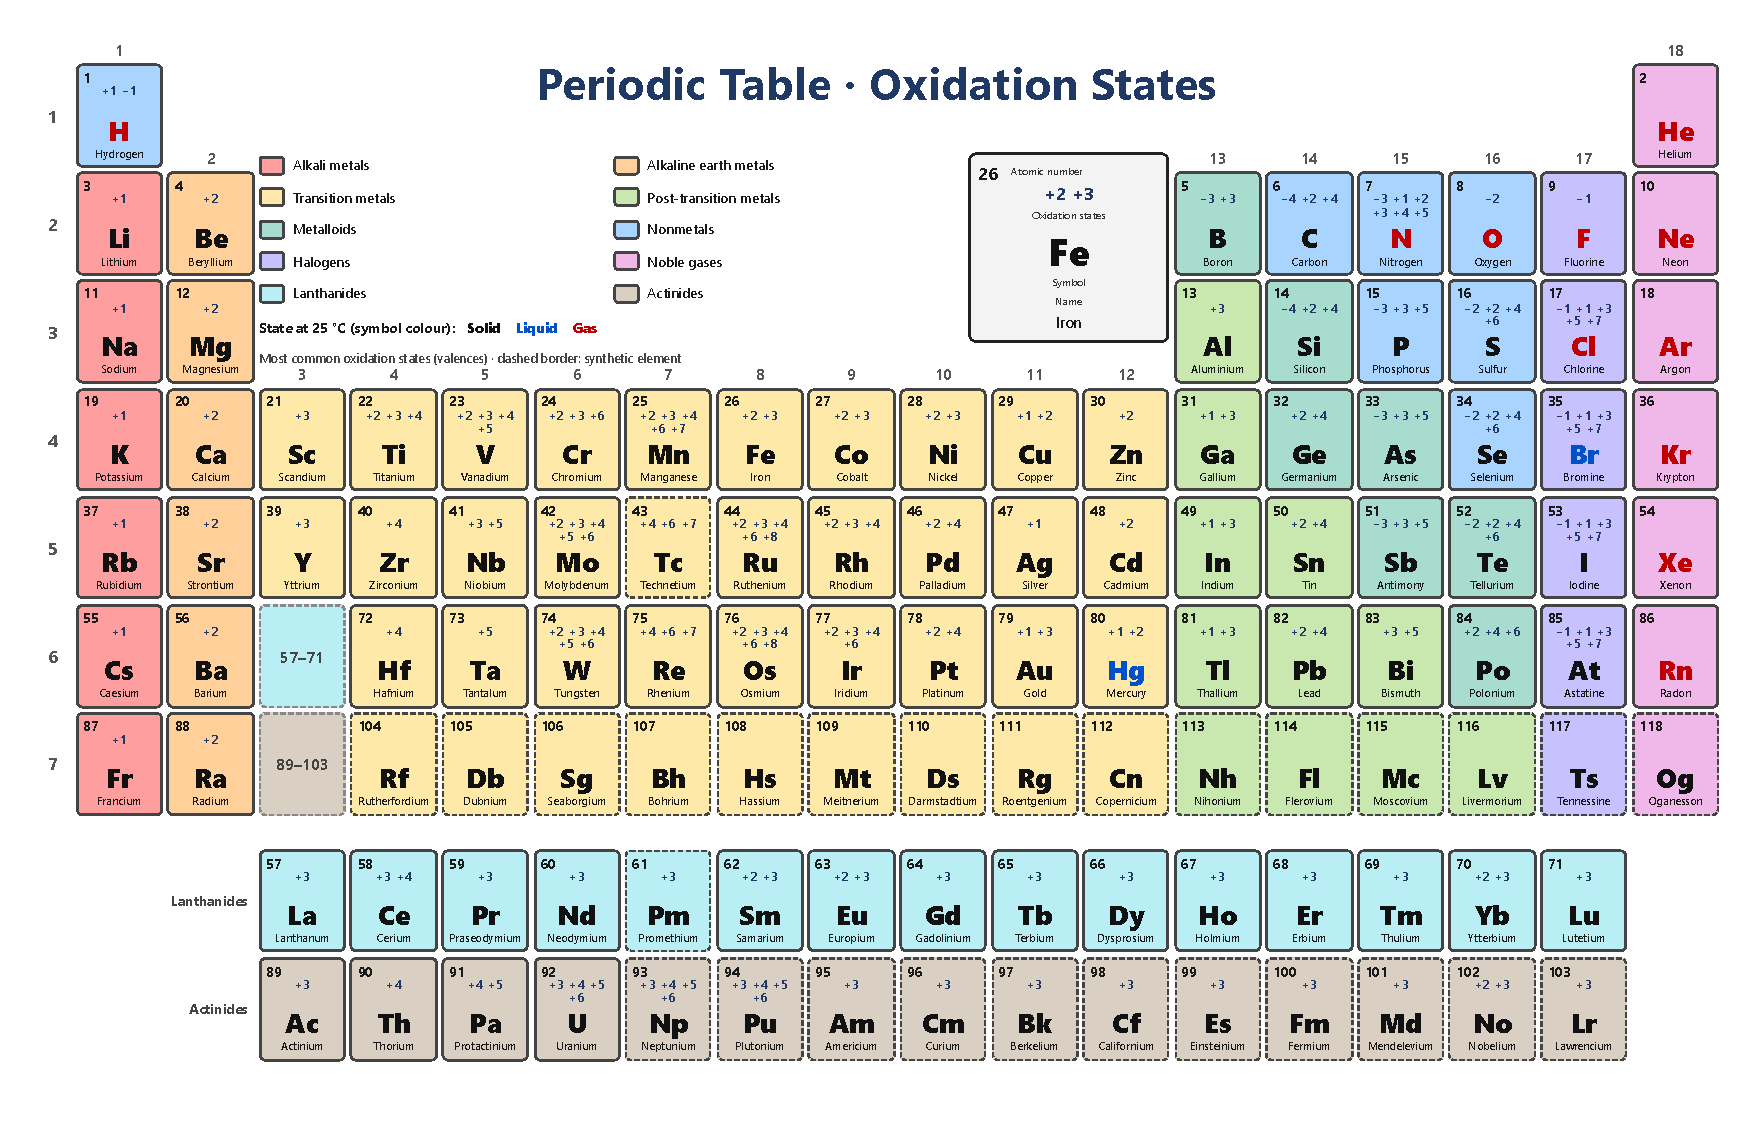
\includegraphics[width=\linewidth,height=0.85\textheight,keepaspectratio]{images/TP_Valencias_EN_html}
        \caption{Periodic Table: oxidation states}
        \label{fig:tabla_valencias}
    \end{figure}
\end{landscape}
    \newpage
    \begin{landscape}

    \begin{figure}[H]
        \centering
        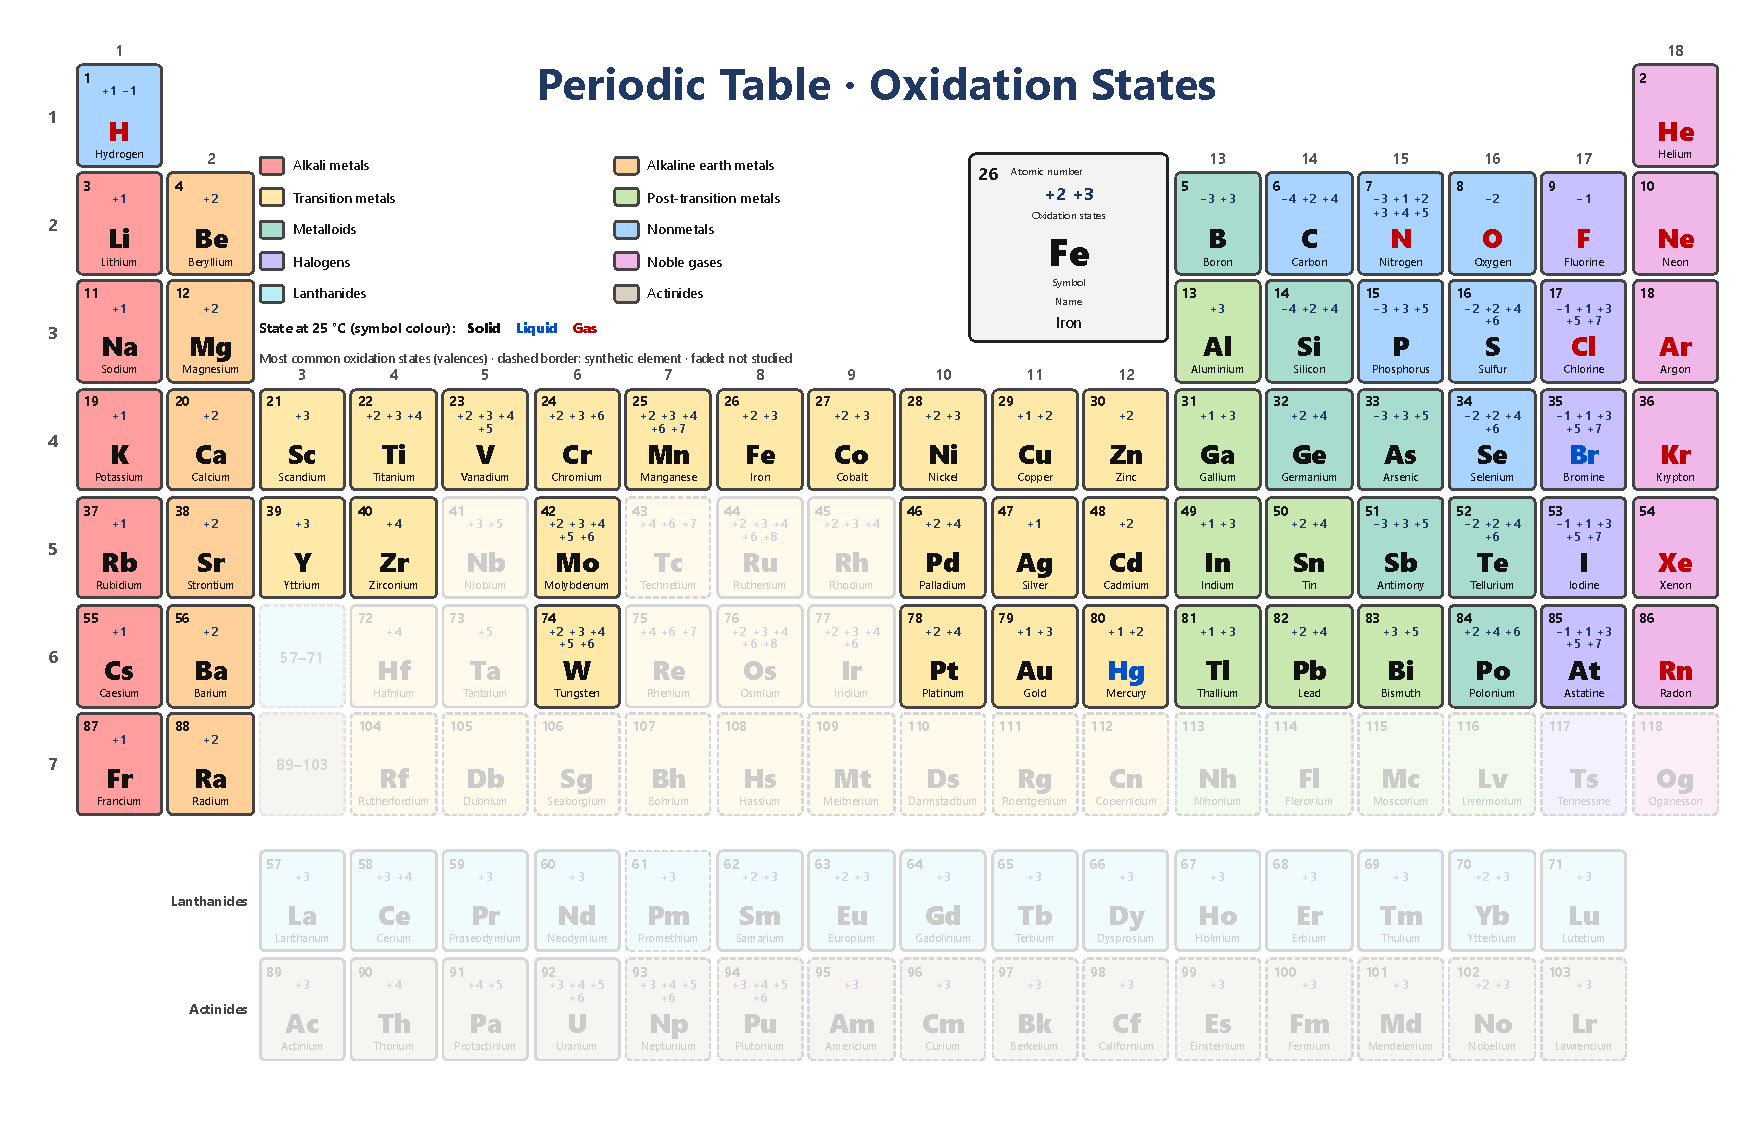
\includegraphics[width=\linewidth,height=0.85\textheight,keepaspectratio]{images/TP_Valencias_EN_reducida_html}
        \caption{Periodic Table: oxidation states (2º ESO)}
        \label{fig:tabla_valencias_reducida}
    \end{figure}
\end{landscape}
    \pagestyle{fancy}

%----------------------------------------------------------------------------------------
%	SOLUTIONS
%----------------------------------------------------------------------------------------


    \part{Solutions to the exercises}

    \chapterimage{images/portada_cabeceras/cabecera_general}
    \chapter{Solutions} % las soluciones van agrupadas por capítulo (secciones)

    \Closesolutionfile{ans}
%
    \input{soluciones}


\end{document}
